\documentclass[themecolor=brown]{textbook-cn}
\graphicspath{{./figure/}{./figures/}{./image/}{./images/}{./graphics/}{./graphic/}{./pictures/}{./picture/}}%提供多种图片路径
\makeatletter
%%设计封面%%
\newcommand{\ifetdef}{
\maxsizebox{\paperwidth}{!}{\ifdefvoid{\@englishtitle}{}{\@englishtitle}}
}
\newcommand{\makecover}{
\tikzset{coverup node/.style={text=ColorA,anchor=north west,inner sep=0mm},
coverdown node/.style={text=white,anchor=west,inner sep=0mm},
opacity node/.style={anchor=north west,font=\FontSizeSet{100pt}{120pt}\bfseries\sffamily,text=ColorB!25}
}
\begin{titlepage}
\begin{tikzpicture}[remember picture,overlay]
\coordinate(A)at(current page.north west);
\coordinate(B)at(current page.north east);
\coordinate(C)at(current page.south east);
\coordinate(D)at(current page.south west);
\coordinate(E)at([yshift=5.25cm]current page.west);
\coordinate(F)at([yshift=5.25cm]current page.east);
\coordinate(G)at($0.5*(E)+0.5*(C)$);
%%背景1%%
\draw[ColorB!5,fill=ColorB!5,sharp corners](D)rectangle(B);
%%半透明文字%%
\node[opacity node,text opacity=1.0](O_1)at(A){\ifetdef};
\foreach \x[evaluate=\x as \botpoint using int(\x-1),
evaluate=\x as \opa using 1.2-0.2*\x] in {2,...,10}{
\node[opacity node,text opacity=\opa](O_\x)at(O_\botpoint.south west){\ifetdef};}
%%背景2%%
\draw[ColorA!80,fill=ColorA!80](E)rectangle(C);
%%封面图%%
\node[inner sep=0mm,anchor=center](CI)at(G){\ifdefvoid{\@coverimage}{}{\includegraphics[width=\paperwidth,height=\paperheight/2+5.25cm]{\@coverimage}}};
%%标题%%
\node[font=\FontSizeSet{55pt}{66pt}\bfseries\sffamily,coverup node](T)at(current page text area.north west){\@title};
%%英文标题%%
\node[font=\FontSizeSet{20pt}{24pt}\bfseries\sffamily,coverup node](ET)at([yshift=-0.5cm]T.south west){\ifdefvoid{\@englishtitle}{}{\@englishtitle}};
%%副标题%%
\node[font=\FontSizeSet{30pt}{36pt}\bfseries\sffamily,coverup node](ST)at([yshift=-0.5cm]ET.south west){\ifdefvoid{\@subtitle}{}{\@subtitle}};
%%英文副标题%%
\node[font=\FontSizeSet{15pt}{18pt}\bfseries\sffamily,coverup node](EST)at([yshift=-0.5cm]ST.south west){\ifdefvoid{\@englishsubtitle}{}{\@englishsubtitle}};
%%作者%%
\node[font=\FontSizeSet{15pt}{18pt}\bfseries\sffamily,coverdown node](A)at([yshift=4.0cm]current page text area.west){主编\quad\@author};
%%出版社%%
\node[coverdown node](PL)at(current page text area.south west){\ifdefvoid{\@presslogo}{}{\includegraphics[width=0.75cm]{\@presslogo}}};
\node[font=\FontSizeSet{15pt}{18pt}\bfseries\sffamily,coverdown node](PN)at([xshift=0.25cm]PL.east){\ifdefvoid{\@pressname}{}{\@pressname}};
\end{tikzpicture}
\end{titlepage}}

%%设计封底%%
\newcommand{\ifestdef}{
\maxsizebox{\paperwidth}{!}{\ifdefvoid{\@englishsubtitle}{}{\@englishsubtitle}}
}
\NewDocumentCommand{\makeback}{ +O{} o }{
\tikzset{backup node/.style={text=ColorA,anchor=north east,inner sep=0mm,text width=\textwidth},
backdown node/.style={text=white,anchor=west,inner sep=0mm},
opacity node/.style={anchor=north east,font=\FontSizeSet{100pt}{120pt}\bfseries\sffamily,text=ColorB!25}}
\begin{titlepage}
\begin{tikzpicture}[remember picture,overlay]
\coordinate(A)at(current page.north west);
\coordinate(B)at(current page.north east);
\coordinate(C)at(current page.south east);
\coordinate(D)at(current page.south west);
\coordinate(E)at([yshift=5.25cm]current page.west);
\coordinate(F)at([yshift=5.25cm]current page.east);
\coordinate(G)at($0.5*(E)+0.5*(C)$);
%%背景1%%
\draw[ColorB!5,fill=ColorB!5,sharp corners](D)rectangle(B);
%%半透明文字%%
\node[opacity node,text opacity=1.0](O_1)at(B){\ifestdef};
\foreach \x[evaluate=\x as \botpoint using int(\x-1),
evaluate=\x as \opa using 1.2-0.2*\x] in {2,...,10}{
\node[opacity node,text opacity=\opa](O_\x)at(O_\botpoint.south east){\ifestdef};}
%%背景2%%
\draw[ColorA!80,fill=ColorA!80](E)rectangle(C);
%%封底图%%
\node[inner sep=0mm,anchor=center](BI)at(G){\ifdefvoid{\@backimage}{}{\scalebox{1}[1]{\includegraphics[width=\paperwidth,height=\paperheight/2+5.25cm]{\@backimage}}}};
%%条形码%%
\IfValueTF{#2}{
\node[draw=white,fill=white,inner xsep=0mm,anchor=south east](BC)at([yshift=-0.5cm]current page text area.south east){\includegraphics[width=5.0cm]{#2}};}{\relax}
%%说明文字%%
\node[font=\ChapterSayingFont,backup node](BT)at(current page text area.north east){\hspace*{2.0em}#1};
%%书籍系列%%
\node[font=\FontSizeSet{15pt}{18pt}\bfseries\sffamily,backdown node](S)at([yshift=4.0cm]current page text area.west){\ifdefvoid{\@series}{}{\@series}};
%%书籍系列%%
\node[font=\FontSizeSet{15pt}{18pt}\bfseries\sffamily,backdown node](V)at([yshift=-0.5cm]S.south west){\ifdefvoid{\@version}{}{第{\@version}版}};
\end{tikzpicture}
\end{titlepage}}

%%设计书脊%%
\NewDocumentCommand{\makespine}{O{1.0cm}}{
\newlength{\SpineWidth}
\setlength{\SpineWidth}{#1}
\tikzset{spine title/.style={font=\FontSizeSet{20pt}{24pt}\bfseries\sffamily,text=white,text width=1.0cm,align=center},
spine subtitle/.style={font=\FontSizeSet{15pt}{18pt}\bfseries\sffamily,text=white,text width=1.0cm,align=center},
spine englishtitle/.style={font=\FontSizeSet{20pt}{24pt}\bfseries\sffamily,text=ColorA,inner sep=0mm}}
\begin{titlepage}
\begin{tikzpicture}[remember picture,overlay]
\coordinate(A)at(current page.north);
\coordinate(B)at(current page.south);
\coordinate(C)at([yshift=5.25cm]current page.center);
%%背景%%
\draw[ColorB!5,fill=ColorB!5]
([xshift=-\SpineWidth/2]A)rectangle([xshift=\SpineWidth/2]B);
\draw[ColorA!80,fill=ColorA!80]
([xshift=-\SpineWidth/2]C)rectangle([xshift=\SpineWidth/2]B);
%%书脊英文标题%%
\node[spine englishtitle,anchor=north](ET)at([yshift=-0.5cm]A){\ifdefvoid{\@englishtitle}{}{\rotatebox[origin=c]{-90}{\maxsizebox{\paperheight/2-5.25cm}{\SpineWidth}{\@englishtitle}}}};
%%书脊标题%%
\node[spine title,anchor=north](T)at([yshift=-0.5cm]C){\@title};
%%书脊副标题%%
\node[spine subtitle,anchor=north](ST)at([yshift=-0.5cm]T.south){\ifdefvoid{\@subtitle}{}{\@subtitle}};
%%书脊出版社名称%%
\node[spine subtitle,anchor=south](PN)at([yshift=0.5cm]B){\ifdefvoid{\@pressname}{}{\@pressname}};
%%书脊出版社logo%%
\node[spine subtitle,anchor=south](PL)at([yshift=0.25cm]PN.north){\ifdefvoid{\@presslogo}{}{\includegraphics[width=0.8cm]{\@presslogo}}};
\end{tikzpicture}
\end{titlepage}}
\makeatother
\makeatletter


\NewDocumentCommand{\Logo}{O{0.5}mmm}{
\def\globalscale{#1}
\begin{tikzpicture}[y=1.0pt,x=1.0pt,yscale=-\globalscale,xscale=\globalscale,every node/.append style={scale=\globalscale},inner sep=0pt,outer sep=0pt]
\path[draw,draw opacity=0,left color=ColorB,right color=ColorA,even odd rule,line width=0pt,miter limit=8.0] (291.5,56.6) .. controls (372.9,58.3) and (460.0,93.2) .. (530.6,159.7) .. controls (572.1,198.8) and (603.1,244.2) .. (622.9,291.6) -- (623.6,293.4) -- (616.4,280.9).. controls (600.2,254.0) and (579.9,228.7) .. (555.6,205.8) .. controls (426.2,83.9) and (232.6,79.3) .. (123.1,195.5) .. controls (78.7,242.7) and (55.0,302.6) .. (51.1,365.2) -- (50.7,377.5) -- (47.8,365.6) .. controls (28.4,279.0) and (46.0,192.0) .. (103.8,130.6) .. controls (152.0,79.5) and (219.5,55.1) .. (291.5,56.6) -- cycle;
\draw[white,line width={\globalscale*10.0pt},fill=ColorH](600,270)circle(50);
\node[font=\bfseries\sffamily\FontSize{90},text=white,inner sep=0mm](P)at(600,270){\maxsizebox{1.5cm}{!}{#4}};
\node[font=\bfseries\sffamily\FontSize{90},text=ColorH,anchor=north,inner xsep=0mm,minimum height=2.0cm](T)at(315,190){\maxsizebox{12.0cm}{!}{\MakeUppercase{#2}}};
\node[font=\bfseries\sffamily\FontSize{150},text=ColorA,anchor=north,inner xsep=0mm,minimum height=4.0cm](S)at([yshift=30]T.south){\maxsizebox{16.0cm}{!}{\MakeUppercase{#3}}};
\draw[ColorB,line width={\globalscale*10.0pt},line cap=round]([xshift=-20,yshift=20]S.south west)--([xshift=20,yshift=20]S.south east);
\end{tikzpicture}}

\makeatother


\makeatletter

%%选择题的4个选项,根据选项内容长度自动排版%%
\colorlet{ListColor}{ColorA}
\newlength{\la}
\newlength{\lb}
\newlength{\lc}
\newlength{\ld}
\newlength{\lhalf}
\newlength{\lquarter}
\newlength{\lmax}
\newcommand{\choice}[4]{
\settowidth{\la}{A.~#1~~~}
\settowidth{\lb}{B.~#2~~~}
\settowidth{\lc}{C.~#3~~~}
\settowidth{\ld}{D.~#4~~~}
\ifthenelse{\lengthtest{\la>\lb}}
{\setlength{\lmax}{\la}}{\setlength{\lmax}{\lb}}
\ifthenelse{\lengthtest{\lmax<\lc}}
{\setlength{\lmax}{\lc}}{\relax}
\ifthenelse{\lengthtest{\lmax<\ld}}
{\setlength{\lmax}{\ld}}{\relax}
\setlength{\lhalf}{0.5\linewidth}
\setlength{\lquarter}{0.25\linewidth}
\ifthenelse{\lengthtest{\lmax>\lhalf}}
{\begin{hlist}[pre skip=0pt,item skip=0pt,item offset={1.5em},label={\textbf{\color{ListColor}{\Alpha{hlisti}.}}},pre label={}]1
\hitem #1
\hitem #2
\hitem #3
\hitem #4
\end{hlist}}
{\ifthenelse{\lengthtest{\lmax>\lquarter}}
{\begin{hlist}[pre skip=0pt,item skip=0pt,item offset={1.5em},label={\textbf{\color{ListColor}{\Alpha{hlisti}.}}},pre label={}]2
\hitem #1
\hitem #2
\hitem #3
\hitem #4
\end{hlist}}
{\begin{hlist}[\parskip=0pt,pre skip=0pt,item skip=0pt,item offset={1.5em}, label={\textbf{\color{ListColor}{\Alpha{hlisti}.}}},pre label={}]4
\hitem #1
\hitem #2
\hitem #3
\hitem #4
\end{hlist}}
}}


\makeatother


\usepackage{zhlipsum,lipsum}%乱数假文(测试文字)
\usepackage{physics}%物理符号包
\usepackage{siunitx}%物理符号包
\usepackage{tabularx,colortbl,array,tabularray,booktabs,multirow}%表格
\usepackage{wrapfig}%文字环绕图片
\usetikzlibrary{3d}

\usepackage{pdfpages}

%\usepackage[cam,cross,letter,center]{crop}


%%设置书籍信息%%
\seriesname{物理学系列教程}
\serieslogo{Springer.pdf}
\version{一}
\title{物理学基础讲义}
\englishtitle{Fundamental of Physics}
\subtitle{经典力学与热力学}
\englishsubtitle{Classical Mechanics \& Thermal Dynamics}
\author{【美】吉尔·沃克\\【美】大卫·哈里德\\【美】罗伯特·瑞斯尼克\\【中】N·A·S·A}
\pressname{中等教育出版社}
\presslogo{bookpresslogo.pdf}

%空心字母
\newcommand{\E}{\mathbb{E}}
\renewcommand{\Pr}{\mathbb{P}}
\newcommand{\EP}{\mathbb{E}^{\mathbb{P}}}
\newcommand{\EQ}{\mathbb{E}^{\mathbb{Q}}}
\newcommand{\dif}{\,{\rm d}}
\newcommand{\Var}{{\rm Var}}
\newcommand{\Cov}{{\rm Cov}}

%旧式正切余切函数名 tan cot tanh coth arctan arccot
\newcommand{\sh}{\operatorname{sh}}
\newcommand{\ch}{\operatorname{ch}}
\renewcommand{\th}{\operatorname{th}}
\newcommand{\tg}{\operatorname{tg}}
\newcommand{\ctg}{\operatorname{ctg}}
\newcommand{\tgh}{\operatorname{tgh}}
\newcommand{\ctgh}{\operatorname{ctgh}}
\newcommand{\arctg}{\operatorname{arctg}}
\newcommand{\arcctg}{\operatorname{arcctg}}

%龟壳括号,又称六角括号
\newcommand{\lbr}{\ensuremath{\lbrbrak}}
\newcommand{\rbr}{\ensuremath{\rbrbrak}}
\newcommand{\lhbrak}{\ensuremath{\lbrbrak}}
\newcommand{\rhbrak}{\ensuremath{\rbrbrak}}

%表格对齐设置
\newcolumntype{M}{>{\centering\arraybackslash}X}
\newcolumntype{Z}{>{\raggedright\arraybackslash}X}
\newcolumntype{Y}{>{\raggedleft\arraybackslash}X}

\newcommand{\inputlogo}[1]{\raisebox{-0.5em}{\includegraphics[width=1.5cm]{#1}}~~}
%%
\newcommand{\Hinputlogo}[2]{\href{#2}{\inputlogo{#1}}}


%%%%%%%%%%%%%%%%%%%%%%%%%%%%%%%%%%%%%%%%%%%%%%%%%%%%%%%%%%%%%%%%%%%%%%%%%%%%%%%%%%%
\begin{document}
\MainFont



%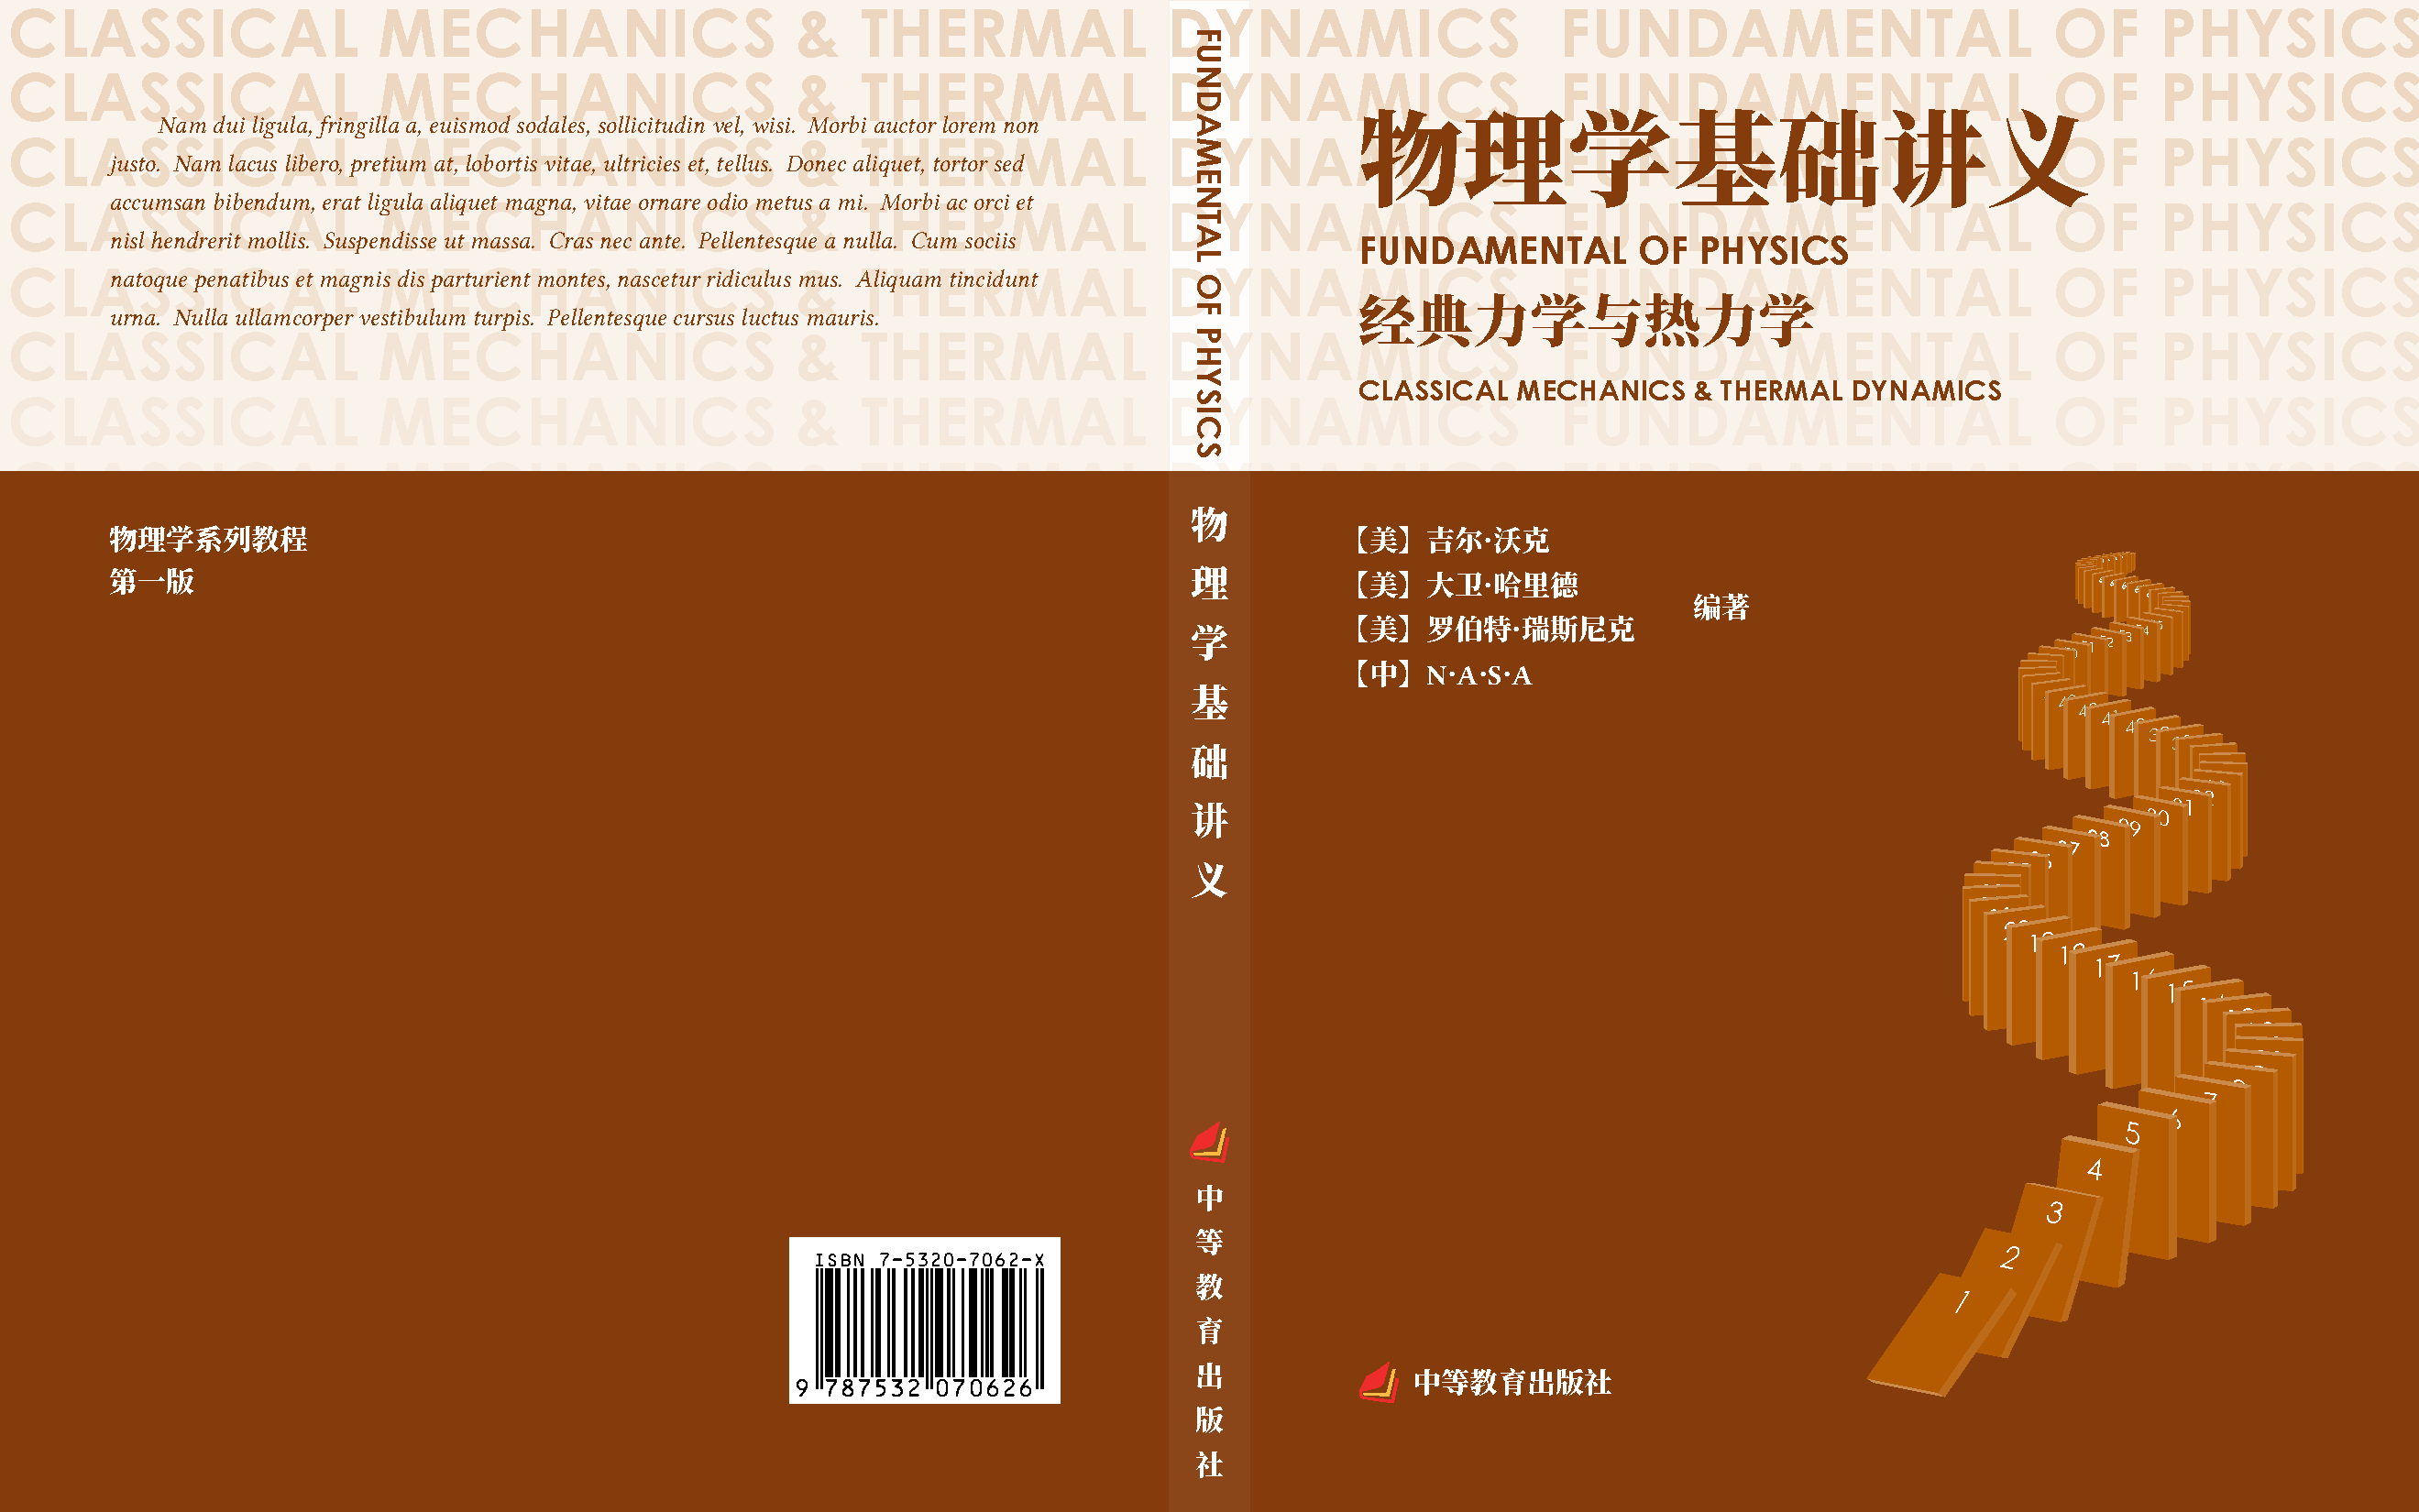
\includepdf{bookcover.pdf}

\maketitle
% 内容提要

% 内容提要
    这套书是沃克、哈里德和瑞斯尼克所著《物理学原理》(Principles of Physics)第10版的中译本。它是一部不仅在美国高校中使用率高,而且在世界许多国家的大学中广泛使用的国际经典教材。
    
    全套书的特点是:突出物理概念,物理原理和定理表述严谨、准确,内容广泛联系最新的科学研究、生产实际以及日常生活。书中除包含传统教科书中经典物理学的全部内容外,第37章到第44章还简要介绍了近代物理学的主要进展,包括相对论、量子物理学,最后一章还提到了夸克和大爆炸。关于引力的第13章,详细讨论了牛顿的引力理论,还简单介绍了等效原理和弯曲时空。书中有许多来自生活和新科技的生动有趣的例子,对提高学生学习物理学的兴趣、明确学习物理学的目的大有裨益。
    
    全套书分上、下两卷,共44章,上卷从第1章到第20章;下卷从第21章到第44章。为了能更好地帮助学生理解和领会物理学的原理和概念,书中每章第一单元的开头都安排有“什么是物理学”的栏目,强调这一章中的主要物理内容。每章中的每单元均设有“学习目标”和“关键概念”的栏目,列出学生学完该单元后必须掌握的物理内容及物理概念。书中的例题分成若干小题,每一小题都详细地交代了解题的关键概念和解题步骤。每章都附有丰富的习题以供教师和学生选择。
    
    本套书的插图内容丰富,表意清楚,制作精美,与正文配合密切。本套书可用作高等学校基础物理课的教材或参考书,同时也是广大教师(包括中学教师)、物理科研人员和物理爱好者十分有价值的参考书。
    
		
\thispagestyle{empty}
\lipsum[1-6]



\frontmatter
\lipsum
% 序言



\chapter{前言}




%\subsubsection*{我为什么要写这本书}


面对巨大的挑战很有乐趣。这是我对学物理的看法。这想法来自那一天,我曾教的一位名叫莎伦的学生(现已毕业)突然问我:“在我的生活中,这些东西有什么用呢?”当然我立即回答说:“莎伦,在你的生活中每件事都和这有关——这就是物理学。”

她要我举一个例子,我想来想去就是想不出一个合适的。那个晚上我就开始写《物理学的飞行马戏团》(John Wiley \& Sons公司,1975)。这本书是为莎伦而写,也是为我自己而写,因为我知道她的疑问也是我的疑问。我花了六年时间认真钻研了几十本物理学教科书,这些书都是根据最好的教学计划认真地编写出来的,但都缺少了某些东西。物理学是最有趣的学科之一,因为它是关于自然界是怎样运行的,但这些教科书完全没有谈到和真实自然界的任何关系,有趣的东西也都一点没有了。

我已经在《物理学原理》这本书中采纳了从新版的《物理学的飞行马戏团》中挑选出来的许多真实世界物理学的例子。许多材料来自我教的物理学导论课程。在这些课上,我可以从学生的面部表情和直率的评论判断哪些材料和展示有好的效果,而哪些却没有。我的成功和失败记录是形成这本书的基础。这里我要传达的信息和多年前遇到莎伦以来我给我遇到过的每一位学生传达的都同样是:“你们从基本的物理概念终究可以推导出有关真实世界的合理的结论,这种对真实世界的认识就是乐趣之所在。”

我写这本书有好几个目标,但首要的目标是给教师提供一些工具,他们据此可以教学生如何有效地阅读科学资料,懂得基本概念,思考科学问题,并且能够定量地解题。无论对学生还是教师来说,这个过程并不容易。确实,使用这本书的课程或许是学生学过的所有课程中最具挑战性的一门课。然而,它也可能是最值得做的一件事,因为它揭示了所有科学和工程应用赖以实现的自然界的基本机理。

本书第9版的许多使用者(包括教师和学生)给我提出了改进本书的批评意见和建议。这些改进都体现在全书的叙述和习题中。出版商John Wiley \& Sons公司和我把这本书看作不断发展的项目并鼓励使用者提出更多的意见。你们可以把建议、修改意见以及正面或负面的意见送交John Wiley \& Sons或吉尔·沃克(通信地址:克利夫兰州立大学物理系,Cleveland,OH44115 USA);或博客地址:www.flying circus of physics.com)。我们可能无法对所有的建议都做出回应,但我们会尽量保留并研究每一条建议。\footnote{看看我}


\subsubsection*{哪些是新的东西?}
\paragraph{单元和学习目标}“我要从这一节学习到什么?”几十年来最好的学生和最差的学生都问过我这个问题。问题在于,即使是一个善于思考的学生在阅读一个小节时,对是否抓住了要点也可能会感到没有信心。回想起我在用第1版哈里德和瑞斯尼克合著的《物理学》教第一学年的物理学课程时也有同样的感受。

在这一版中为使这个问题缓解一些,我在原来题目的基础上把各章重组成概念的单元,并将各单元的学习目标列出作为每个单元的开始。这些列出的项目是对阅读这一单元应当学到的要点和技巧的简明表述。紧接着每一组列项是对应当学到的关键概念的简明小结。例如,看一看第16章第一单元,学生在这一单元中要面临一大堆的概念和名词。我现在提供了明晰的检索清单,学生可以靠自己的能力把这些概念收集和分类,它的作用就好像飞行员起飞前在跑道上滑行时要通盘核对一遍程序表格一样。

\paragraph{课外作业习题和学习目标之间的关系}
在WileyPLUS中,每一章后面的每一个问题和习题都联系着学习目标,要回答(通常不用说出来)这样的问题:“我为什么要做这个习题?我应该从它学到什么?”通过明确一个习题的目的,我相信学生会用不同的语言但却相同的关键概念把学习目标更好地转移到其他的习题上。这种转移有助于克服常常遇到的困难,就是学生学会了解某一特殊的习题,但却不会把它的关键概念用于另一种条件下的问题。

\paragraph{重写某几章}我的学生对关键的几章和另外几章中的一些方面不断地提出建议,所以在这一版中我重写了许多内容。例如,我重新构思了关于高斯定律和电势这两章,因为原先的这两章被证明对我的学生来说太困难了。现在的表述更加流畅,并且关键的要点表述更加直截了当。在有关量子物理的几章里,我扩展了薛定谔方程的范围,包括物质波在阶跃势上的反射。遵照一些教师的要求,我将玻尔原子的讨论和氢原子的薛定谔解分开,这样就可以绕过对玻尔工作的历史说明。还有,现在有了关于普朗克的黑体辐射的单元。

\paragraph{新的例题}16个新的例题已经被增加到各章中,这是为了突出我的学生们感到困难的一些领域。

\paragraph{可视图解}在WileyPLUS中可以得到这本教材的电子版,这是罗格斯大学(Rutgers University)的戴维·梅洛(David Maiullo)制作的教材中大约30幅照片和插图的视频。物理学中大部分是研究运动的事物,视频常常可以比静态的照片和图片提供更佳的描述。

\paragraph{在线辅助}WileyPLUS不仅仅是在线评分的程序,实际上它还是生动的学习中心,配有许多不同的学习辅助材料,包括实时的解题指导、鼓励学生的嵌入式阅读测验、动画、几百道例题、大量的模拟和演示以及1500个以上的视频,内容从数学复习到与例题有关的微型课程。每学期都会增加更多的学习辅助材料。在《物理学原理》第10版中,一些运动的照片被转换成视频,这样可以将运动变慢以进行分析。

这几千个学习辅助材料可以全天候得到,并且可以随意重复使用。这样,如果一个学生,譬如说在半夜2点40分(这好像是做物理课外作业的最佳时间)被一个课外作业题难住,点击鼠标就可以得到合适的、对他有帮助的资料。

\subsubsection*{学习工具}
当我用第1版哈里德和瑞斯尼克合著的《物理学》学习第一年物理学时,我通过反复阅读才得以理解每一章。现今,我们更好地了解到,学生有广泛多样的学习风格,所以我制作了多样的学习工具,这些都体现在了这一版的书和在线的WileyPLUS中。

\paragraph{动画}每一章都有一些关键的图用动画表现。在这本书中,这些图用旋涡符号来标记。在WileyPLUS的线上章节中,点击鼠标动画就开始了。我选择其中有丰富信息的一些图做成动画,故学生可以看到的不仅仅是那些印刷在书页上的插图,而是活生生的物理学,并且用几分钟时间就可以播放完。这不但使物理学鲜活起来,而且动画可以根据学生的需要多次重复播放。

\paragraph{视频}我已经制作了1500多个教学视频,每学期还要增加,学生可以听我在解释、指导、讲解例题或总结的时候在屏幕上看着我画图或打字,十分像他们在我的办公室里坐在我旁边看我在草稿本上推算某些东西时的经历一样。教师的讲课或个别指导总是最有价值的学习方式,而我们视频是全天候都可以得到的,并且可以无数次地重复使用。

\begin{UnnumberedItem}
\item 一些章节中某些主题的视频辅导。我选择学生感到最困难、最伤脑筋的一些主题。

\item 高中数学的视频复习,像基本的代数运算、三角函数和联立方程。

\item 数学的视频介绍,像矢量运算,这对学生来说是新的知识。

\item 教材各章中每个例题的视频图像描述。我的意图是从关键概念出发学习物理学而不是只抓住公式。然而,我还是会演示怎样解读例题,就是说怎样读懂技术资料,学会解题的步骤,这些也可以用到其他类型的习题上。

\item 每一章后面20\% 的习题的视频求解。学生是不是能够看到这些解以及什么时候才能得到答案是由教师控制的。例如,可以在课外作业截止期限以后或者小测验以后得到。每一个解答不是简单的对号入座的处方。我建立了从基本概念和推理的第一步开始到最后的答案的解题方法。学生不仅仅是学习解答一道特定的习题,而是要学会处理任何问题,甚至要有处理这些问题所需要的物理学的勇气。

\item 怎样从曲线图读出数据的视频例子(并不是在没有理解物理意义的情况下就去简单地读取数字)。
\end{UnnumberedItem}




\paragraph{解题助手}我已经为WileyPLUS编写了大量的资料,这些是为帮助学生提高解题能力而设计的。

\begin{UnnumberedItem}
\item 本书中的每道例题的阅读及视频版本都可以在线上得到。

\item 几百道附加的例题。这些都是独一无二的资料,但(可由教师自己选定)它们也连接着超出课外作业范围的例题。所以,如果一道课外作业题是处理,比如说是作用于斜面上的木块的力,那么这里也提供了有关例题的连接。不过,这种例题和课外作业并不完全一样,它并不提供一个只要复制而不用理解的解答。

\item 每一章后面的课外作业中的15\% 都可在GO Tutorials栏目中找出求解步骤。我引导学生做课外作业要经过多个步骤,从关键概念开始,有时给出错误的答案并做出提示。然而,我会故意把(得到最终答案的)最后一步留给学生。这样,他们最后要自己负责做完习题。某些在线教学系统有意给出错误答案让学生落入陷阱,这会使学生产生很大的困惑,而我的GO Tutorials并不是陷阱,学生在解题过程中的每一步都可以回到主要的问题上来。

\item 每一章后面课外作业的每一道题的提示都可以(在教师的指导下)得到。我编写的这些材料是关于主要概念和解题一般步骤的具体提示,而不是只提供答案而无须理解的诀窍。
\end{UnnumberedItem}

\paragraph{评价资料}

\begin{UnnumberedItem}
\item 在线上的每一节都可找到相应的阅读问题。我编写这些材料并不是要让他们进行分析或深入的理解,只是为了测试一下学生是不是读过这一节。当学生打开某一节时,从题库中随机选择的阅读问题就会出现在该节最后的空白处。教师可以自行决定这个问题是作为打分数的根据呢,还是仅仅作为学生的练习。在线上的每一节都可找到相应的阅读问题。我编写这些材料并不是要让他们进行分析或深入的理解,只是为了测试一下学生是不是读过这一节。当学生打开某一节时,从题库中随机选择的阅读问题就会出现在该节最后的空白处。教师可以自行决定这个问题是作为打分数的根据呢,还是仅仅作为学生的练习。

\item 在大多数小节中设置有检查点。这些检查点要求用这一节中的物理原理做分析和判断。所有检查点的答案都在书的最后。

\item 本书中每一章后面的大多数习题(和更多其他的习题)在WileyPLUS中都可以找到。教师可以在线上指定课外作业,并依据网上提交的答案打分。例如,教师规定交作业的截止日期和允许一个学生对一个答案可以尝试多少次。教师也可以控制每一道课外习题能得到哪些学习帮助(如果有的话)。这种连接包括提示、例题、章内的阅读材料、视频辅导、视频教学复习,甚至还包括视频解题(这可以在课外作业截止日期后给学生)。

\item 符号标记的习题。这种需要得到代数式答案的习题在每章中都有。
\end{UnnumberedItem}




\subsubsection*{教师用的补充资料}

\paragraph{教师用解题手册}由Lawrence Livermore国家实验室的Sen-Ben Liao编著。这本手册提供每章后面所有习题的解题步骤,它有MS Word和PDF两种格式。

\paragraph{教师伴侣网址}http://www.wiley.com/college/halliday

\paragraph{教师手册}这份资料概括了每一章中最重要的论题的讲课要点、演示实验、实验室和计算机项目、电影和视频资料、所有习题的答案和检查点以及与以前版本中习题相关的指导,也包含了学生可以得到解答的所有习题的完整目录。

\paragraph{讲课用Power Point幻灯片}这些Power Point幻灯片可用作对教师有帮助的起动包,它概括了这本教材中的关键概念和相关的图表及方程式。

\paragraph{Wiley物理学模拟}由Boston University的Andrew Duffy和Vernier Software的John Gastineau制作。这是50个相互作用的模拟(Java应用程序),可以用作课堂演示。

\paragraph{Wiley物理学演示}由Rutgers University的David Maiullo制作。这是80个标准物理学演示的数字视频的集合。它们可以在课堂上演示或从WileyPLUS中得到。另有与选择题相配套的教师指导。

\paragraph{试题库}第10版的试题库已被Northern Illinois University的Suzanne Willis全部检查过,试题库包含2200多道多项选择题。这些题目在计算机试题库中也可找到,这个计算机试题库提供了完整的编辑功能,可以帮助你按自己的要求选择测验题(IBM和Macintosh版本都可以得到)。

\paragraph{教材中所有的图表}适用于课堂投影或印刷。


\paragraph{线上课外作业和小测验}除了WileyPLUS和《物理学原理》第10版外,也支持WebAssign PLUS和LON-CAPA,这些程序也提供教师在线上布置课外作业和小测验以及评分的功能。WebAssignPLUS也给学生提供这本教材的线上版本。

\subsubsection*{学生用的补充资料}
\paragraph{学生伴侣}网址http://www.wiley.com/college/hallidy,这是专门为《物理学原理》第10版制作并为进一步帮助学生学习物理学而设计的,它包含每一章后面的部分习题的解答、模拟练习,以及怎样最好地应用可编程计算器的技巧。

\paragraph{互动学习软件}这个软件指导学生如何求解200道各章后面的习题。求解过程是互动的,有适当的反馈并可得到防止最常见错误的具体指导。




















\shorttableofcontents
\tableofcontents

\listoffigures


\cleardoublepage

\lipsum[2]


\mainmatter


\partintro{\lipsum[2]}
\part[短标题]{力学}
\lipsum
%% 第一章



%\begin{Appendix}


\begin{Appendix}

\chapter{附录}
\lipsum

\chapter{附录}
\section{附录测试}

\end{Appendix}

\begin{Appendix}
	
\section{附录测试}

\section{附录测试}

\section{附录测试}
	
\end{Appendix}




\begin{Appendix}
	
\section{附录测试}
	
\end{Appendix}



\begin{Project}

%\begin{Topic}
\section{测量物体,包含长度测量}

\section{测量物体,包含长度测量}
%\end{Topic}

\chaptersaying{文王拘而演周易,仲尼厄而作春秋。}
\chapter{测量}

\zhlipsum

\section{测量物体,包含长度测量}

\section{测量物体,包含长度测量}

\section{测量物体,包含长度测量}



\end{Project}




\begin{Project}

\section{测量物体,包含长度测量}

\begin{Point*}
	学习完这一单元,你应当能够: 识别国际单位制(SI)中的基本量; 正确称呼国际单位制中最常用的词头; 利用链环变换法改变单位(这里是对于长度、面积和体积); 说明米是如何用真空中光速来定义的。
	\tcblower
	\tcbsubtitle{本节重点}
	物理学是以物理量的测量为基础的。一些物理量被选作基本物理量; 每一种基本物理量都已经通过一种标准来定义并给定测量的单位。另一些物理量是用这些基本物理量和它们的标准及单位来定义。
	
	本书主要用的单位制是国际单位制(SI)。基本物理量的标准必须都是可以得到并且是不变的,这些基本量的标准都已经通过国际协议确立了。这些标准用在所有的物理测量中,基本量和从这些基本量导出的量都是如此。
	
	单位的变换可以通过链环变换法来完成,在这种变换法中,将原来的数据连续乘以统一协调的变换因子,单位要像代数量一样处理,直到留下所要求的单位。

	米定义为在精确规定的时间间隔内光通过的路程。
\end{Point*}


%\begin{Case*}
%
%\end{Case*}



\begin{Paracol}
	\subsection{什么是物理学?}
	\NoteArea
	
	科学和工程学建立在测量和比较的基础上。因此,我们就需要关于如何测量和比较物体的规则,并且我们还需要通过实验来建立这种测量和比较的单位。物理学(以及工程学)的一个目的就是设计和实施这些实验。
	
	例如,物理学家们尽力开发极其准确的时钟从而使任何时间或时间间隔都可以精确地确定和比较。你们可能要问,这样的准确度是否真正需要,或者是否值得花这么大的精力。这里给出一个是否值得的例子:如果没有极其准确的时钟的话,那么现在全世界范围的航行必不可少的全球定位系统(GPS)就会变得毫无意义。
	
	\subsection{测量物体}
	\NoteArea
	
	\subsubsection{测试文字}
	
	我们通过学习怎样测量物理学中的量来学习物理学。这些物理量包括长度、时间、质量、温度、压强和电流。
	
	我们通过和一个标准相比较,用它们各自的单位来量度各个
	
	
	
	
	
\end{Paracol}

\subsection{力的三要素}


\subsubsection{测试文字}

力是有大小的.我们在初中学过,力的大小可以用测力计来测量.在国际单位制中力的单位是\textbf{牛顿},简称牛,国际符号是N,日常生活和生产中常用的力的单位是千克力,牛顿和千克力的关系是:1千克力$=9.8$牛.

力不但有大小,而且有方向.物体受到的重力是竖直向下的,物体在液体中受到的浮力是竖直向上的,力的方向不同,它的作用效果也不同.用力拉弹簧,弹簧就伸长;用反方向的力压弹簧,弹簧就缩短.作用在运动物体上的力,如果方向与运动方向相同,将加快物体的运动;如果方向与运动方向相反,将阻碍物体的运动.可见,要把一个力完全表达出来,除了说明力的大小外,还要指明力的方向.

\begin{wrapfigure}[6]{r}{6cm}
	\vspace*{-1.5em}
	\centering
	\begin{tikzpicture}[>=stealth, thick]
		\draw (0,0)--(2,0)--(2,1)--(0,1)--(0,0);
		\fill [pattern = north east lines] (-1,-.75) rectangle (3,-.5);
		\draw(-1,-.5)--(3,-.5);
		\draw (.5,-.25) circle (.225);
		\draw (1.5,-.25) circle (.225);
		\draw (.5,-.25) circle (.1);
		\draw (1.5,-.25) circle (.1);
		\draw[->, dashed](3,0.5)--(-2,0.5);
		\draw[very thick](0,.5)--(-2,0.5);
		\foreach \i in {-.4,-.8,-1.2,-1.6,-2}
		{
			\draw (\i,0.6)--(\i,.5);
		}
		\draw (-1,1)--(-1,1.1);
		\draw (-0.6,1)--(-0.6,1.1);
		\draw[-] (-1,1)--(-0.6,1);
		\node at (-0.8,1.35){$\qty{20}{N}$};
	\end{tikzpicture}
	\caption{图中的虚线表示力的作用线}
\end{wrapfigure}
为了直观地说明力的作用,常常用一根带箭头的线段来表示力.线段是按一定比
例(标度)画出的,它的长短表示力的大小,它的指向表示力的方向,箭头或箭尾表示力的作用点,箭头所沿的直线叫做力的作用线.这种表示力的方法,叫做\textbf{力的图示}.图1.1中表示的是作用在小车上的$\qty{100}{N}$的力.

\subsection{力的分类}

我们从初中开始学习物理以来,见过的力的名称已经相当多了.各种力可以用不同的方法来分类.一种是根据力的性质来分类的,如重力、弹力、摩擦力、分子力、电磁力等;另一种是根据力的效果来分类的,如拉力、压力、支持力、动力、阻力等等.拉力、压力、支持力实际上都是弹力,只是效果不同.不论是什么性质的力,只要效果是加快物体的运动,就可以叫它为动力;效果是阻碍物体的运动,就可以叫它为阻力.今后我们还会遇到根据效果来命名的力的名称.

从力的性质来看,力学中经常遇到的有重力、弹力、摩擦力.下面几节就分别介绍这三种力.


\begin{Example}
	测试文字测试文字测试文字测试文字测试文字测试文字测试文字测试文字测试文字测试文字测试文字测试文字测试文字测试文字测试文字测试文字测试文字测试文字测试文字测试文字测试文字测试文字测试文字测试文字测试文字测试文字测试文字测试文字测试文字测试文字测试文字测试文字测试文字测试文字测试文字测试文字测试文字测试文字测试文字测试文字测试文字
	\begin{flalign}
		\Psi=\int_\Omega\left[f\left(\phi\right)+\kappa\left|\nabla\phi\right|^2\right]{\rm d}V
	\end{flalign}
\end{Example}

\begin{Example}
	测试文字测试文字
\end{Example}


\subsection{测试文字}
\subsection*{测试文字}
\zhlipsum[1]




\makeatletter



\makeatother

\begin{multicols}{2}
\Basis

\Complex
\end{multicols}

\zhlipsum[1]

















\clearpage

\Improve
\begin{QuestionItem}[2]
	\item 关于行星运动的规律,下列说法符合史实的是
	\choice{开普勒在牛顿定律的基础上,导出了行星运动的规律}{开普勒在天文观测数据的基础上,总结出了行星运动的规律}{开普勒总结出了行星运动的规律,找出了行星按照这些规律运动的原因}{开普勒总结出了行星运动的规律,发现了万有引力定律}
	\item 火星和木星沿各自的椭圆轨道绕太 阳运行,根据开普勒行星运动定律可知
	\choice{太阳位于木星运行轨道的中心}{火星和木星绕太阳运行速度的大小始终相等}{火星与木星公转周期之比的平方等于它们轨道半长轴之比的立方}{相同时间内,火星与太阳连线扫过的面积等于木星与太阳连线扫过的面积}
	\item 为了探测引力波,“天琴计划” 预计发射地球卫星P,其轨道半径约为地球半径的16倍;另一地球卫星Q的轨道半径约为地球半径的4倍。P与Q的周期之比约为
	\choice{2∶1}{4∶1}{8∶1}{16∶1}
	\item 测试文字测试文字测试文字测试文字测试文字测试文字测试文字测试文字测试文字测试文字测试文字测试文字测试文字测试文字测试文字测试文字测试文字测试文字测试文字测试文字测试文字测试文字测试文字测试文字测试文字测试文字测试文字测试文字测试文字测试文字测试文字测试文字测试文字测试文字测试文字测试文字测试文字测试文字测试文字测试文字测试文字测试文字测试文字测试文字测试文字测试文字测试文字测试文字
	\item 测试文字测试文字测试文字测试文字测试文字测试文字测试文字测试文字测试文字测试文字测试文字测试文字测试文字测试文字测试文字测试文字测试文字测试文字测试文字测试文字测试文字测试文字测试文字测试文字测试文字测试文字测试文字测试文字测试文字测试文字测试文字测试文字测试文字测试文字测试文字测试文字测试文字测试文字测试文字测试文字测试文字测试文字测试文字测试文字测试文字测试文字测试文字测试文字
	\item 测试文字测试文字测试文字测试文字测试文字测试文字测试文字测试文字测试文字测试文字测试文字测试文字测试文字测试文字测试文字测试文字测试文字测试文字测试文字测试文字测试文字测试文字测试文字测试文字测试文字测试文字测试文字测试文字测试文字测试文字测试文字测试文字测试文字测试文字测试文字测试文字测试文字测试文字测试文字测试文字测试文字测试文字测试文字测试文字测试文字测试文字测试文字测试文字
	\item 测试文字测试文字测试文字测试文字测试文字测试文字测试文字测试文字测试文字测试文字测试文字测试文字测试文字测试文字测试文字测试文字测试文字测试文字测试文字测试文字测试文字测试文字测试文字测试文字测试文字测试文字测试文字测试文字测试文字测试文字测试文字测试文字测试文字测试文字测试文字测试文字测试文字测试文字测试文字测试文字测试文字测试文字测试文字测试文字测试文字测试文字测试文字测试文字
	\item 测试文字测试文字测试文字测试文字测试文字测试文字测试文字测试文字测试文字测试文字测试文字测试文字测试文字测试文字测试文字测试文字测试文字测试文字测试文字测试文字测试文字测试文字测试文字测试文字测试文字测试文字测试文字测试文字测试文字测试文字测试文字测试文字测试文字测试文字测试文字测试文字测试文字测试文字测试文字测试文字测试文字测试文字测试文字测试文字测试文字测试文字测试文字测试文字
	\item 测试文字测试文字测试文字测试文字测试文字测试文字测试文字测试文字测试文字测试文字测试文字测试文字测试文字测试文字测试文字测试文字测试文字测试文字测试文字测试文字测试文字测试文字测试文字测试文字测试文字测试文字测试文字测试文字测试文字测试文字测试文字测试文字测试文字测试文字测试文字测试文字测试文字测试文字测试文字测试文字测试文字测试文字测试文字测试文字测试文字测试文字测试文字测试文字
	\item 测试文字测试文字测试文字测试文字测试文字测试文字测试文字测试文字测试文字测试文字测试文字测试文字测试文字测试文字测试文字测试文字测试文字测试文字测试文字测试文字测试文字测试文字测试文字测试文字测试文字测试文字测试文字测试文字测试文字测试文字测试文字测试文字测试文字测试文字测试文字测试文字测试文字测试文字测试文字测试文字测试文字测试文字测试文字测试文字测试文字测试文字测试文字测试文字
	\item 测试文字测试文字测试文字测试文字测试文字测试文字测试文字测试文字测试文字测试文字测试文字测试文字测试文字测试文字测试文字测试文字测试文字测试文字测试文字测试文字测试文字测试文字测试文字测试文字测试文字测试文字测试文字测试文字测试文字测试文字测试文字测试文字测试文字测试文字测试文字测试文字测试文字测试文字测试文字测试文字测试文字测试文字测试文字测试文字测试文字测试文字测试文字测试文字
	\item 测试文字测试文字测试文字测试文字测试文字测试文字测试文字测试文字测试文字测试文字测试文字测试文字测试文字测试文字测试文字测试文字测试文字测试文字测试文字测试文字测试文字测试文字测试文字测试文字测试文字测试文字测试文字测试文字测试文字测试文字测试文字测试文字测试文字测试文字测试文字测试文字测试文字测试文字测试文字测试文字测试文字测试文字测试文字测试文字测试文字测试文字测试文字测试文字
	\item 测试文字测试文字测试文字测试文字测试文字测试文字测试文字测试文字测试文字测试文字测试文字测试文字测试文字测试文字测试文字测试文字测试文字测试文字测试文字测试文字测试文字测试文字测试文字测试文字测试文字测试文字测试文字测试文字测试文字测试文字测试文字测试文字测试文字测试文字测试文字测试文字测试文字测试文字测试文字测试文字测试文字测试文字测试文字测试文字测试文字测试文字测试文字测试文字
	\item 测试文字测试文字测试文字测试文字测试文字测试文字测试文字测试文字测试文字测试文字测试文字测试文字测试文字测试文字测试文字测试文字测试文字测试文字测试文字测试文字测试文字测试文字测试文字测试文字测试文字测试文字测试文字测试文字测试文字测试文字测试文字测试文字测试文字测试文字测试文字测试文字测试文字测试文字测试文字测试文字测试文字测试文字测试文字测试文字测试文字测试文字测试文字测试文字
	\item 测试文字测试文字测试文字测试文字测试文字测试文字测试文字测试文字测试文字测试文字测试文字测试文字测试文字测试文字测试文字测试文字测试文字测试文字测试文字测试文字测试文字测试文字测试文字测试文字测试文字测试文字测试文字测试文字测试文字测试文字测试文字测试文字测试文字测试文字测试文字测试文字测试文字测试文字测试文字测试文字测试文字测试文字测试文字测试文字测试文字测试文字测试文字测试文字
	\item 测试文字测试文字测试文字测试文字测试文字测试文字测试文字测试文字测试文字测试文字测试文字测试文字测试文字测试文字测试文字测试文字测试文字测试文字测试文字测试文字测试文字测试文字测试文字测试文字测试文字测试文字测试文字测试文字测试文字测试文字测试文字测试文字测试文字测试文字测试文字测试文字测试文字测试文字测试文字测试文字测试文字测试文字测试文字测试文字测试文字测试文字测试文字测试文字
\end{QuestionItem}


\Thinking
	\begin{QuestionItem}
		\item 测试文字测试文字测试文字测试文字测试文字测试文字测试文字测试文字测试文字测试文字测试文字测试文字测试文字测试文字测试文字测试文字测试文字测试文字测试文字测试文字测试文字测试文字测试文字测试文字测试文字测试文字测试文字测试文字测试文字测试文字测试文字测试文字测试文字测试文字测试文字测试文字测试文字测试文字测试文字测试文字测试文字测试文字测试文字测试文字测试文字测试文字测试文字测试文字
		\item 测试文字测试文字测试文字测试文字测试文字测试文字测试文字测试文字测试文字测试文字测试文字测试文字测试文字测试文字测试文字测试文字测试文字测试文字测试文字测试文字测试文字测试文字测试文字测试文字测试文字测试文字测试文字测试文字测试文字测试文字测试文字测试文字测试文字测试文字测试文字测试文字测试文字测试文字测试文字测试文字测试文字测试文字测试文字测试文字测试文字测试文字测试文字测试文字
		\item 测试文字测试文字测试文字测试文字测试文字测试文字测试文字测试文字测试文字测试文字测试文字测试文字测试文字测试文字测试文字测试文字测试文字测试文字测试文字测试文字测试文字测试文字测试文字测试文字测试文字测试文字测试文字测试文字测试文字测试文字测试文字测试文字测试文字测试文字测试文字测试文字测试文字测试文字测试文字测试文字测试文字测试文字测试文字测试文字测试文字测试文字测试文字测试文字
		\item 测试文字测试文字测试文字测试文字测试文字测试文字测试文字测试文字测试文字测试文字测试文字测试文字测试文字测试文字测试文字测试文字测试文字测试文字测试文字测试文字测试文字测试文字测试文字测试文字测试文字测试文字测试文字测试文字测试文字测试文字测试文字测试文字测试文字测试文字测试文字测试文字测试文字测试文字测试文字测试文字测试文字测试文字测试文字测试文字测试文字测试文字测试文字测试文字
	\end{QuestionItem}


\begin{Definition}[测试文字]
	测试文字
	\begin{flalign}
		\Psi=\int_\Omega\left[f\left(\phi\right)+\kappa\left|\nabla\phi\right|^2\right]{\rm d}V
	\end{flalign}
\end{Definition}

\begin{Lemma}
	测试文字
\end{Lemma}

\begin{Theorem}[测试文字]
	测试文字
\end{Theorem}

\begin{Axiom}[测试文字][测试文字]
	测试文字
\end{Axiom}


\begin{Proposition}
	测试文字
\end{Proposition}


\begin{Corollary}
	测试文字
\end{Corollary}

\begin{Lemma}
	测试文字
\end{Lemma}


\begin{Lemma*}[测试文字测试文字]
	测试文字测试文字测试文字测试文字测试文字测试文字测试文字测试文字测试文字测试文字
	
	测试文字测试文字测试文字测试文字测试文字测试文字测试文字测试文字测试文字测试文字
	\zhlipsum
	测试文字测试文字测试文字测试文字测试文字测试文字测试文字测试文字测试文字测试文字测试文字测试文字
	\tcblower
	\tcbsubtitle{测试文字}
	\zhlipsum[2]
	\tcbsubtitle{副标题}
	\zhlipsum[2]
\end{Lemma*}


\begin{multicols}{3}
\Subheading{测试文字}
测试文字测试文字测试文字测试文字测试文字测试文字测试文字测试文字测试文字测试文字测试文字测试文字测试文字测试文字测试文字
\Subheading{测试文字}
测试文字测试文字测试文字测试文字测试文字测试文字测试文字测试文字测试文字测试文字测试文字测试文字测试文字测试文字测试文字
\Subheading{测试文字}
测试文字测试文字测试文字测试文字测试文字测试文字测试文字测试文字测试文字测试文字测试文字测试文字测试文字测试文字测试文字
\end{multicols}


\Heading{练习题}

\begin{UnnumberedItem}[3]

\item test
\item test
\item test
\item test
\item test
\item test
\item test
\item test
\item test
\end{UnnumberedItem}

\begin{NumberedItem}
	\item 测试文字
	\item test
	\item testqjply
\end{NumberedItem}



\begin{Proof}
	\lipsum[1]
	\tcblower
	\lipsum
\end{Proof}

\begin{Block}%[测试文字]
	\lipsum[1]
	\tcblower
	\lipsum
\end{Block}


\begin{Check}
	\lipsum[1-2]
	\tcbline
	\lipsum[1-2]
\end{Check}

\begin{Warning}
	\lipsum[2]
	\tcbsubtitle{测试文字}
	\tcblower
	\tcbsubtitle{测试文字}
	cswz
\end{Warning}



\begin{Vocabulary}
	\lipsum
\end{Vocabulary}



\Remark{\lipsum[2][1-3]}

\begin{PythonBox}[神经网络]
import pytorch as pt
import numpy as np
import pandas as pd
\end{PythonBox}

\end{Project}







%\begin{Quiz}

\section{测试文字}

\makeatletter
\@SubsectionStarStyle{测试文字}{测试文字}
\makeatother
\lipsum



\subsection{测试文字}
\subsubsection{测试文字}


\subsection{测试文字}
\subsubsection{测试文字}


\begin{Example}
	测试文字测试文字测试文字测试文字测试文字测试文字测试文字测试文字测试文字测试文字测试文字测试文字测试文字测试文字测试文字测试文字测试文字测试文字测试文字测试文字测试文字测试文字测试文字测试文字测试文字测试文字测试文字测试文字测试文字测试文字测试文字测试文字测试文字测试文字测试文字测试文字测试文字测试文字测试文字测试文字测试文字
	\begin{flalign}
		\Psi=\int_\Omega\left[f\left(\phi\right)+\kappa\left|\nabla\phi\right|^2\right]{\rm d}V
	\end{flalign}
\end{Example}




\Improve
\begin{QuestionItem}[2]
	\item test$\Psi=\int_\Omega\left[f\left(\phi\right)+\kappa\left|\nabla\phi\right|^2\right]{\rm d}V$
	\item test
	$$\Psi=\int_\Omega\left[f\left(\phi\right)+\kappa\left|\nabla\phi\right|^2\right]{\rm d}V$$
	\item test
	\item test
	\item test
	\item test
	\item test
	\item test
\end{QuestionItem}


\Thinking
\begin{QuestionItem}
	\item 测试文字
	\item 测试文字
	\item 测试文字
	\item 测试文字
\end{QuestionItem}


%\end{Quiz}




\section{测试文字}

\section{测试文字}


\chapter{测试文字}

\section{测试文字}

\section{测试文字}



\begin{Appendix}
	
\chapter{测试计数器}
	
\section{附录测试}
	
\end{Appendix}

\chapter{中间}

\begin{Appendix}

\chapter{测试}
	
\section{附录测试}
	
\end{Appendix}





%\end{Appendix}



%% 第二章
%\chapter{直线运动}


\begin{Topic}

\section{机械运动}

我们在初中学过,一个物体相对于另一个物体的位置变化叫做\textbf{ 机械运动},简称运动.在自然界中没有不动的物体.房屋、桥梁、树术、山岭等总在原地不动,我们说它们是静止的.其实它们是随着地球一起运动的,不但地球在运动,太阳在银河系中也是运动的.小到原子和分子,大到宇宙中的天体,一切物体都在运动,机械运动是宇宙中最普遍的现像.
\subsection{参照物}
既然一切物体都在运动,我们研究一个物体的运动时,就必须选取另外的物体作为参照,事先假定这个另外的物体是不动的,这样才能进行研究;我们说房屋、桥梁等是静止的,行驶的汽车是运动的,这是选取地面作为参照来说的;房屋、桥梁等对地面来说位置没有发生变化,行驶的汽车对地面来说位置发生了变化.坐在行驶的火车车厢里的乘客认为自己是静止的,在车厢里走动的乘务员是运动的,这是选取车厢作为参照来说的;乘客对车厢来说位置没有发生变化,乘务员对车厢来说位置发生了变化.研究物体的运动时,选来作为参照的另外的物体,叫做\textbf{ 参照物}.

原则上,研究一个物体的运动时,参照物是可以任意选取的.观察在河里游泳的人的运动,可以选择河岸作参照物,也可以选择在河上航行的船只作参照物,研究天体的运动时,可以取地球作参照物,也可以取太阳作参照物.但是,实际选取参照物时,往往要考虑研究问题的方便,使运动的描述尽可能简单.例如,研究太阳系的行星运动,太阳是最理想的参照物.研究地面上物体的运动,一般说来取地面做参照物比较方便.

\subsection{平动和转动}

物体的运动一般是比较复杂的,但是最基本的运动只有两种:平动和转动.

从桌内拉出抽屉的时候,抽屉各部分的运动轨迹完全相同,也就是说,各部分的运动完全相同.这样的运动就是\textbf{ 平动}.打桩时重锤的下落运动,汽缸里活塞的运动,车床上车刀(图2.1)的运动,在直铁轨上行驶的火车车厢的运动,都是平动.
\begin{figure}[H]
    \centering
    \begin{tikzpicture}[>=stealth,line join=round,scale=1.39]
        \pgfdeclareverticalshading{pile}{100bp}{color(0bp)=(black);color(50bp)=(white);color(100bp)=(black)}
        % \draw (0,0)rectangle(6,4.5);
        \coordinate (A) at ([shift=(-155:0.2)]-0.8,-0.9);
        \coordinate (B) at ([yshift=0.2cm]A);
        \draw[very thick](-2.0,-0.9)--(-2.8,-0.9)--++(45:0.3)--++(-0.1,0)coordinate(C);
        \fill[top color=brown,bottom color=brown,middle color=white]([yshift=0.3mm]C)--([xshift=-3mm,yshift=0.4mm]C)to[bend right]++(0,-0.08)--([yshift=-0.3mm]C);
        \draw[fill=gray!70]([shift=(25:1.2)]0,-1.15)--++(-155:2.4)--++(0.2,0)--++(25:2.4);
        \draw[fill=darkgray]([shift=(25:1.2)]0.2,-1.15)--++(-155:2.4)--++(0,-0.3)--++(25:2.4);
        \draw[fill=gray!70]([shift=(25:1.2)]0.5,-1.15)--++(-155:2.4)--++(0.2,0)--++(25:2.4);
        \draw[fill=darkgray]([shift=(25:1.2)]0.7,-1.15)--++(-155:2.4)--++(0,-0.3)--++(25:2.4);
        \draw[fill=lightgray!30]([shift=(-155:1.2)]0,-1.15)rectangle++(0.2,-0.3);
        \draw[fill=lightgray!30]([shift=(-155:1.2)]0.5,-1.15)rectangle++(0.2,-0.3);
        \draw[fill=lightgray!40,very thin](-1,-1.15)--(0.7,-1.15)--(0.7,-1.35)--(0.8,-1.35)--(0.8,-1.05)--(-1,-1.05);
        \draw[fill=gray!40,very thin](-1,-1.05)--(0.8,-1.05)--++(25:0.3)--++(-1.7,0);
        \draw[fill=darkgray!40,very thin](0.8,-1.05)--++(25:0.3)--++(0,-0.3)--++(-155:0.3);
        \draw[very thin,fill=lightgray](-0.8,-0.9)--++(-1.8,0)--++(25:0.4)--++(1.8,0);
        \draw[very thin,fill=gray](-0.8,-0.9)--++(-1.8,0)--++(0,-0.2)--++(1.8,0);
        \draw[very thin,fill=lightgray](B)--++(-1.2,0)--++(25:0.8)--++(1.2,0)--cycle;
        \draw[very thin,fill=darkgray](B)--++(25:0.8)--++(0,-0.4)--++(-155:0.8)--cycle;
        \draw[very thin,fill=gray](B)rectangle++(-1.2,-0.4);
        \draw[very thin,fill=lightgray](-0.8,-0.9)--++(0.5,0)--++(25:0.4)--++(-0.5,0);
        \draw[very thin,fill=gray](-0.8,-0.9)rectangle++(0.5,-0.2);
        \draw[very thin,fill=darkgray](-0.3,-0.9)--++(0,-0.2)--++(25:0.4)--++(0,0.2);
        \draw[very thin,fill=darkgray](-1.05,-0.25)--++(25:0.1)--++(0,-0.2)--++(-155:0.1);
        \draw[very thin,fill=lightgray](-0.9,-0.2)--++(25:0.5)--++(-0.5,0)--++(-155:0.5)--cycle;
        \draw[very thin,fill=darkgray](-0.9,-0.2)--++(25:0.4)--++(0,-0.15)--++(-155:0.4)--cycle;
        \draw[fill=gray,very thin](-0.9,-0.2)rectangle(-1.4,-0.35);
        \draw[very thin,fill=darkgray](-1.05,-0.35)--(-1.05,-0.25)--++(-155:0.8)--++(0,-0.2)--++(25:0.8);
        \draw[very thin,fill=lightgray](-1.05,-0.25)--++(-0.2,0)--++(-155:0.8)--++(0.2,0);
        \draw[very thin,fill=gray]([shift=(-155:0.8)]-1.05,-0.25)rectangle++(-0.2,-0.2);
        \draw[very thin,fill=lightgray](-1.4,0.05)--(-0.3,0.05)--++(25:0.1)--++(-1.1,0)--cycle;
        \draw[very thin,fill=lightgray](-0.2,0)--++(25:0.1)--++(-0.1,0.05)--++(-155:0.1)--cycle;
        \fill[left color=gray,right color=gray,middle color=white,draw=black,very thin](-1.1,0.2)--(-1.1,-0.1)arc(180:360:0.1 and 0.05)--(-0.9,0.2);
        \draw[very thin,fill=gray](-0.95,-0.05)--(-0.3,-0.05)--(-0.2,0)--(-0.3,0.05)--(-0.95,0.05);
        \draw[very thin,fill=gray](-1.05,-0.05)--(-1.4,-0.05)--(-1.4,0.05)--(-1.05,0.05);
        \fill[lightgray,draw=black,very thin](-1,0.2)ellipse(0.1 and 0.05);
        \draw [shading=pile,shading angle=25](115:0.2)--++(25:1.0)arc(115:-65:0.2)--++(-155:1.0)--cycle;
        \draw[fill=lightgray](0,0)circle(0.2);
        \draw[thin,postaction={decorate},decoration={markings,mark={at position 0.7 with{\arrow{Stealth[scale=0.5]}}}}](240:0.28)arc(240:300:0.28);
        % \fill(-1.875,-0.7)circle(1pt);
        \draw[very thick](-1.875,-0.688)--++(-155:0.1)--++(-65:0.3)--++(-155:0.1)coordinate(D);
        \fill[top color=brown,bottom color=brown,middle color=white]([shift=(115:0.03)]D)--([shift=(-165:0.3)]D)to[bend right]([shift=(-145:0.3)]D)--([shift=(115:-0.03)]D);
        \draw[thin,->](-0.3,0.3)--++(25:0.5);
        \draw[thin](25:1.0)--++(135:0.5)node[left]{工件};
        \draw[thin](-0.5,0)--++(135:0.6)node[left]{车刀};
    \end{tikzpicture}
    \caption{车床上车刀的平动和工件的转动}
\end{figure}

物体的平动不一定都沿着直线进行,也可以沿曲线进行,图2.2所示的铅笔的平动就是沿着曲线进行的.
\begin{figure}[H]
    \begin{floatrow}
        \ffigbox[0.4\textwidth]{
            \begin{tikzpicture}[decoration={markings,
                            mark=between positions 0.1 and 1 step 0.2 with
                                {\pic {pencil};}}]
                \tikzset{
                    pencil/.pic={
                            \fill[left color =green!80!black,right color=green!80!black,middle color=white](-0.05,0)rectangle(0.05,1.5);
                            \fill(-0.05,1.5)--(0,1.7)--(0.05,1.5);
                            \fill[left color =brown,right color=brown,middle color=white](-0.05,1.5)--(-0.02,1.62)--(0.02,1.62)--(0.05,1.5);
                        }
                }
                \useasboundingbox (-0.6,0)rectangle(3,3.8);
                \draw[postaction={decorate}](0,0)..controls(4.3,0.6)and(2.8,1.3)..(-0.5,1.9);
                \draw[thin,dashed](0,0.85)..controls(4.3,1.45)and(2.8,2.15)..(-0.5,2.75);
                \draw[thin,dashed](0,1.7)..controls(4.3,2.3)and(2.8,3.0)..(-0.5,3.6);
            \end{tikzpicture}
        }{\caption{沿曲线进行的平动}}
        \ffigbox[0.45\textwidth]{
            \begin{tikzpicture}[>=stealth]
                \fill [brown](-1,-1)rectangle(1,0);
                % \draw[thick](-1,0)--(1,0);
                \fill[gray](-0.25,2)rectangle(0.25,0.7);
                \fill[darkgray]
                (0,-0.5)--(0.25,-0.35)..controls(0.25,0.7)and(-0.25,0.7)..(-0.25,1.5)--(-0.25,0.7)..controls(-0.25,0.3)and(0,0.3)..(0,-0.5);
                \fill[top color=gray,bottom color=gray,middle color=white]
                (0,-0.5)..controls(0,0.3)and(-0.25,0.3)..(-0.25,0.7)..controls(-0.25,0.9)and(-0.15,1.2)..(0,1.5)..controls(0.15,1.8)and(0.25,2.0)..(0.25,1.5)--(0.25,0.7)--(0.05,0.7);
                \fill[left color=gray,right color=gray,middle color=white]
                (0.25,0.7)..controls(0.25,0.3)and(0,0.3)..(0,-0.5)--(-0.25,-0.35)..controls(-0.25,0.7)and(0.25,0.7)..(0.25,1.5)--cycle;
                \draw[thick,->](0,1.2)--++(0,-1);
                \fill[lightgray!50](0,2)ellipse(0.25 and 0.1);
                \draw(-0.35,1.7)arc(180:270:0.35 and 0.15);
                \draw[<-](0,1.55)arc(270:360:0.35 and 0.15);
            \end{tikzpicture}
        }{\caption{钻头在工作中同时做平动和转动}}
    \end{floatrow}
\end{figure}
推动石磨的时候,磨盘上的各部分都围绕着通过中心的轴线做圆周运动.这样的运动就是\textbf{ 转动}.脱粒机的滚筒的运动,机器上飞轮的运动,车床上工件的运动(图2.1),都是转动.

在很多情况下,物体同时做平动和转动.钻头在工作的时候(图2.3),车轮在路上滚动的时候,螺栓在拧入螺母中的时候,都是同时做平动和转动的.
\end{Topic}

\begin{Quiz}
\section{质点}

物体都具有大小和形状,在运动中物体中各点的位置变化一般说来是各不相同的,所以要详细描述物体的运动,并不是一件简单的事情.可是,在某些倩况下,却可以不考虑物体的大小和形状,而使问题简化.在这些情形下,我们可以把物体看作一个有质量的点,或者说用一个有质量的点来代替整个物体,用来代替物体的有质量的点叫做\textbf{ 质点}.

在什么情况下可以把物体当作质点,这要看具体倩况而定.举例来说,当我们研究地球的公转时,由于地球的直径(约$\qty{1.3e4}{km}$)比地球和太阳之间的距离(约$\qty{1.5e8}{km}$)要小得多,因而可以忽略地球的大小和形状,把它当作质点,可是研究地球的自转时,我们却不能忽略地球的大小和形状,当然不能把地球当作质点了.

一个平动的物体,它的各个部分的运动情况都相同,它的任何一点的运动都可以代表整个物体的运动.在这种情况下,也可以把整个物体当作质点来看待.一辆在直公路上行驶的汽车,车身上各部分的运动情况相司,当我们把汽车作为一个整体来研究它的运动的时侯,就可以把汽车当作质点.当然,假如我们需要研究汽车的轮胎的运动,由于轮胎的各部分的运动情况不相同,那就不能把它看作质点了.

今后我们研究的物体,除非涉及到转动,一般都可以看作质点.

任何物体都具有一定的大小和形状,因此质点这个概念是一种科学的抽像,是一种理想化的模型.我们研究物体的运动,像研究其他物理现像一样,不能主次不分.如果物体的大小和形状在所研究的现像中起的作用很小,可以忽咯不计,我们就可以把物体看作是一个没有大小和形状的理想物体,即质点.这种研究问题的方法,在物理学中是常常用到的.

研究物体的运动,第一步是要知道物体是怎样运动的,也就是知道物体的运动情况.物体在运动过程中,它的位置和速度不断随时间而变化,如果我们知道了物体在任一时刻的位置和速度,就表示我们知道了物体的运动情况.这一章我们就围绕着这个要求来研究直线运动.

\begin{Exercise}
	\begin{QsNum}
	    \item 两辆在公路上直线行驶的汽车,它们的距离保持不变.试说明用什么样的物体做参照物,两辆汽车都是静止的,用什么样的物体做参照物,两辆汽车都是运动的.能否找到这样一个参照物,一辆汽车时它是静止的,另一辆汽车对它是运动的?为什么?
	
	    \item 小孩从滑梯上滑下,钢球沿斜槽滚下,石块从手中落下,这些物体中哪些是做平动的?
	
	    \item 研完自行车轮的转动,能不能把自行车当作质点?研究在马路上行驶的自行车的速度,能不能把自行车当作质点?
    \end{QsNum}
\end{Exercise}

\end{Quiz}



\begin{Project}
\section{位置与位移}

研究质点的运动,首先要知道怎样确定质点的位置.质点的位置可以采取在数学中学过的建立坐标系的方法来确定.质点做直线运动时,我们可以取这条直线为坐标轴($x$轴),在轴上任选一点$O$为原点,规定好坐标轴的正方向和单位,质点的位置由它的位置坐标,即一个带有正负号的数值,就可以完全确定了.比如我们要确定一辆行驶在北京长安街上的汽车的位置,我们可以取$x$轴表示长安街的东西方向,$x$轴的正方向指东,并且取天安门前的旗杆作为坐标原点,那么汽车的位置就由它的坐标完全确定了.汽车的坐标是$\qty{1}{km}$,表示它在旗杆以东$\qty{1}{km}$处;汽车的坐标是$\qty{-2}{km}$,表示它在旗杆以西$\qty{2}{km}$处(图2.4).
\begin{figure}[H]
    \centering
    \begin{tikzpicture}[>=stealth]
        \tikzset{
            car/.pic={
                    \filldraw[scale=0.5,x=1mm,y=1mm,yscale=-1,xscale=-1,fill=blue!50,xshift=-235,yshift=-90] (59.9429,0.0029) .. controls (58.2798,0.0161) and (56.5224,0.0709) .. (54.6592,0.1699) .. controls (51.8698,0.3182) and (49.2785,0.7036) .. (46.8955,1.2407) .. controls (46.9004,1.2391) and (46.9067,1.2365) .. (46.9116,1.2349) .. controls (35.0588,3.3135) and (25.0020,10.1030) .. (25.0020,10.1030) -- (24.1113,10.1660) .. controls (22.2803,10.1061) and (21.6259,10.2123) .. (17.5122,11.0391) .. controls (15.2265,11.1391) and (13.1653,11.4703) .. (11.3730,11.9180) .. controls (11.2904,11.9383) and (11.2097,11.9609) .. (11.1284,11.9824) .. controls (8.6666,12.6223) and (6.7447,13.4848) .. (5.6074,14.3101) .. controls (2.5699,14.9763) and (0.3984,16.7520) .. (0.3984,16.7520) .. controls (-0.1586,17.2949) and (0.0797,17.2023) .. (0.0044,17.6191) .. controls (-0.0709,18.0360) and (0.7119,21.0322) .. (0.7119,21.0322) .. controls (0.7119,21.0322) and (0.0821,22.9131) .. (0.5215,23.0918) .. controls (0.9609,23.2703) and (1.0903,23.4957) .. (1.4604,24.4233) .. controls (-0.8220,25.6494) and (0.4983,26.3315) .. (1.5059,26.9150) .. controls (2.5136,27.4983) and (5.1650,28.1973) .. (6.5098,27.9229) .. controls (6.4949,27.8726) and (6.4886,27.8209) .. (6.4746,27.7705) -- (8.3862,26.9062) -- (23.4346,26.2646) -- (25.2979,27.3164) .. controls (25.3045,27.3313) and (25.3242,27.3955) .. (25.3242,27.3955) .. controls (25.3242,27.3955) and (25.5918,27.6023) .. (26.2236,27.4849) .. controls (27.8013,27.0856) and (67.5264,26.7188) .. (67.5264,26.7188) .. controls (67.5264,26.7188) and (71.0655,26.7059) .. (72.3955,27.2095) .. controls (72.9263,27.4105) and (73.2239,27.3453) .. (73.4019,27.1245) .. controls (73.7709,27.0085) and (75.1701,26.5817) .. (75.4629,26.5400) .. controls (75.7840,26.4940) and (90.4210,25.8970) .. (90.3750,25.8970) .. controls (90.3293,25.8970) and (92.2559,26.6777) .. (92.2559,26.6777) .. controls (92.2559,26.6777) and (92.3225,26.6082) .. (92.3320,26.5986) .. controls (92.5830,26.6361) and (92.9367,26.6106) .. (93.4336,26.4961) .. controls (95.4068,26.0414) and (96.8291,25.3066) .. (96.8291,25.3066) .. controls (96.8291,25.3066) and (98.1069,23.5919) .. (98.3862,22.9688) .. controls (98.6655,22.3454) and (98.4976,22.1118) .. (98.4976,22.1118) .. controls (98.4976,22.1118) and (98.8375,20.8511) .. (99.2549,19.8252) .. controls (99.6719,18.8000) and (99.6148,18.6385) .. (98.9854,18.0322) .. controls (98.2215,17.0284) and (97.8547,14.8710) .. (98.0010,13.9409) .. controls (98.0616,13.5558) and (98.0431,13.1384) .. (98.0083,12.7661) .. controls (98.0515,11.7298) and (97.7331,10.8516) .. (97.4692,10.3418) .. controls (97.3419,9.9538) and (97.2028,9.5918) .. (97.0620,9.4497) .. controls (96.6727,9.0568) and (97.2353,8.9554) .. (97.7930,8.6543) .. controls (98.3509,8.3530) and (97.8727,8.0535) .. (97.5088,8.0420) .. controls (97.1451,8.0305) and (96.4688,7.9805) .. (96.4688,7.9805) .. controls (95.4388,7.9064) and (92.8843,6.7387) .. (85.3447,4.1309) -- (85.3271,4.1133) .. controls (85.3259,4.1146) and (85.3240,4.1207) .. (85.3228,4.1221) .. controls (85.3044,4.1157) and (85.2943,4.1123) .. (85.2759,4.1060) .. controls (78.6238,1.8073) and (71.5847,-0.0896) .. (59.9429,0.0029) -- cycle;
                    \draw [fill=darkgray] (0,4mm) coordinate (w1)  circle (4mm);
                    \draw [fill=darkgray] (32mm,4mm) coordinate (w2)  circle (4mm);
                }
        }
        \draw [thin,->](-6,0)--(6,0)node[below]{$x$(\si{km})};
        \draw [thin,->](-6,0.8)--(6,0.8);
        \draw [thin,dashed,->](-6,1.1)--(6,1.1);
        \foreach \x in {-5,-4,...,5}
            {
                \draw[thin] (\x,0)--++(0,0.1) node[below=1mm] {$\x$};
            }
        \fill (1,0)circle(1pt);
        \fill (-2,0)circle(1pt);
        \draw[fill=red!80!black](-1.2,1.5)--(1.2,1.5)--(1.1,2.0)--(-1.1,2.0)--cycle;
        \foreach \x in {0.4,0.8,-0.4,-0.8}
            {
                \fill [red!50!brown] (\x-0.1,1.5)--(\x+0.1,1.5)--++(0,0.15)arc(0:180:0.1)--cycle;
            }
        \fill[red!50!brown](-0.12,1.5)--(0.12,1.5)--++(0,0.2)arc(0:180:0.12)--cycle;
        \fill[fill=yellow!80!black](-0.8,2.0)rectangle(0.8,2.05);
        \draw[fill=red!80!black](-0.7,2.05)rectangle(0.7,2.3);
        \foreach \x in {-0.5,-0.3,...,0.5}
            {
                \draw[thick,lightgray](\x,2.05)--(\x,2.3);
            }
        \draw[fill=red!80!black](-0.6,2.35)rectangle(0.6,2.45);
        \draw[fill=yellow!80!black](-0.9,2.3)--(0.9,2.3)--(0.7,2.35)--(-0.7,2.35)--cycle;
        \draw[fill=yellow!80!black](-0.9,2.5)to[bend right=10](-0.6,2.45)--(0.6,2.45)to[bend right=10](0.9,2.5)to[bend left=40](0.6,2.7)--(-0.6,2.7)to[bend left=40]cycle;
        \draw(0,0.5)--(0,3.9);
        \fill[red](0,3.85)to[bend right](-0.7,3.82)--(-0.9,3.25)to[bend left](0,3.22);
        \foreach \x in {-2,1}
            {
                \pic[scale=0.2] at (\x,1.0) {car};
            }
    \end{tikzpicture}
    \caption{}
\end{figure}

\begin{wrapfigure}[8]{r}{5cm}
    \vspace*{-1.5em}
    \centering
    \begin{tikzpicture}[>=stealth,thick]
        \draw [->](0,0)node[left]{$A$} --(3,3)node [right]{$B$} ;
        \draw (0,0) [bend left=-45]  to node [right]{$C$} (3,3);
    \end{tikzpicture}
    \caption{}
\end{wrapfigure}
质点在运动过程中,它的位置随时间不断变化,怎样表示质点的位置变化呢?物理学中用一个叫做\textbf{ 位移}的物理量来表示质点位置的变化.设质点原来在$A$点,经过一段时间沿轨迹$ACB$运动到$B$点(图2.5).从初位置$A$指向末位置$B$作线段$AB$,用它就可以描述质点的位置变化,我们把它叫做质点的位移.$AB$的长度,即位移的大小,表示出位置变化的大小;$AB$的方向,即位移的方向,表示出位置变化的方向.位移既有大小,又有方向,是一个矢量.

位移和路程是两个不同的物理量.路程是指质点所通过的实际轨迹的长度,只有大小,没有方向,是标量.在图2.5中,质点的位移是线段$AB$,而路程是曲线弧${ACB}$的长度,即使在直线运动中位移的大小也不一定等于路程.图2.6表示做直线运动的质点从初位置$A$经过$B$运动到$C$,然后从$C$返回,运动到末位置$B$,这时质点的位移大小是线段$AB$,而路程是线段$AC$的长度加上线段$BC$的长度,只有做直线运动的质点始终向着同一个方向运动时,位移的大小才等于路程.可见,位移矢量一般并不表示运动的实际轨迹和路程,而是表示位置的变化.
\begin{figure}[H]
    \centering
    \begin{tikzpicture}[>=stealth,thick]
        \draw [->](0,0)node[above]{$A$} --(4,0)node [above]{$B$} ;
        \draw (4,0)--(6,0)node [above]{$C$};
        \foreach \x in {0,4,6}
            {
                \draw (\x, -.2)--(\x,.1);
            }
    \end{tikzpicture}
    \caption{}
\end{figure}

在物理学中,通常用$\upDelta x$代表位移.质点做直线运动时,位移可以用末位置的坐标$x$和初位置的坐标$x_0$表示出来:
\begin{equation}
    \upDelta x=x-x_0
\end{equation}


这就是说,位移的数值等于末位置的坐标$x$减去初位置的坐标$x_0$.


在图2.7中,$A$点表示初位置,$B$点表示末位置.图甲中位移:$\upDelta x=x-x_0=\qty{4}{m}-\qty{2}{m}=\qty{2}{m}$,位移是正值,它的大小是$\qty{2}{m}$,方向与坐标轴的正方向相同.图乙中位移:$\upDelta x=x-x_0=\qty{-5}{m}-\qty{1}{m}=\qty{-6}{m}$,位移是负值,它的大小是$\qty{6}{m}$,方向与坐标轴的正方向相反.可见,在直线运动中,用一个带有正负号的数值就可以把位移矢量的大小和方向都表示出来.

\begin{figure}[H]
    \centering
    \begin{tikzpicture}[>=stealth,  thick, scale=1]
        \draw [->](0,0)node[left]{甲} --(14,0)node [below]{$x$(\si{m})} ;
        \foreach \x in {1,2,...,13}
            {
                \draw (\x, 0)--(\x,.2);
            }
        \node at (7,-.5){$O$}; \node at (9,-.5){$x_0=2$}; \node at (11,-.5){$x=4$};
        \draw[->, ultra thick] (9,0) node [above]{$A$}--(11,0)node [above]{$B$};
        \draw [->](0,-2)node[left]{乙} --(14,-2)node [below]{$x$(\si{m})} ;
        \foreach \x in {1,2,...,13}
            {
                \draw (\x, -2)--(\x,-2+.2);
            }
        \node at (7,-2-.5){$O$}; \node at (8,-2-.5){$x_0=1$}; \node at (2,-2-.5){$x=-5$};
        \draw[->, ultra thick] (8,-2) node [above]{$A$}--(2,-2)node [above]{$B$};
    \end{tikzpicture}
    \caption{位移的坐标表示}
\end{figure}

为了方便,在计算位移时常常取初位置为坐标原点,即$x_0=0$.这时质点的位移就可以用末位置的坐标来表示:
\begin{equation*}
    \upDelta x=x
\end{equation*}


\begin{Exercise}
	\begin{QsNum}
	    \item 质点做什么运动,位移的大小才等于路程?
	    \item 图2.6表示做直线运动的质点从初位置$A$经过$B$运动到$C$,然后从$C$返回,运动到末位置$B$.设$AB$长$\qty{7}{m}$,$BC$长$\qty{5}{m}$.求质点的位移的大小和路程.
	    \item 在图2.4中,汽车初位置的坐标是$\qty{-2}{km}$,末位置的坐标是$\qty{1}{km}$.求汽车的位移的大小和方向.
    \end{QsNum}
\end{Exercise}

\end{Project}




\section{匀速直线运动~~速度}
现在我们开始研究物体的运动.从哪里来开始呢?也许从最常见的运动开始比较好吧!一片树叶从树枝上落下是一种很常见的运动,可是仔细观察一下,却发现这种运动很复杂,树叶忽左忽右,有时还发生翻转等,不便于研究.物理学中研究问题常常是从最简单的现像着手.因此,我们从最简单的运动即匀速直线运动来开始对运动的研究.

火车在平直的铁路上行驶,如果它每分钟的位移是$\qty{900}{m}$,每秒钟的位移是$\qty{15}{m}$,也就是在相等的时间内位移相等,这列火车所做的运动就是\textbf{ 匀速直线运动}.

\textbf{ 物体在一条直线上运动,如果在相等时间里的位移相等,这种运动就叫做匀速直线运动}.匀速直线运动有时简称为匀速运动.

飞机在天空中匀速飞行,轮船在海洋上匀速航行,它们的运动虽然都是匀速运动,但还是有区别的.在相同的时间里,飞机的位移大,轮船的位移小,即飞机飞得快,轮船走得慢.在物理学中怎样来表示匀速运动的快慢呢?在匀速运动中,物体在相等时间内的位移相等,因此,如果物体在时间$t$内的位移是$\upDelta x$,在$2t$时间内的位移一定是$2\upDelta x$,在$3t$时间内的位移一定是$3\upDelta x$,等等.可见匀速运动的位移和时间的比值是一个恒量,不随时间而改变.这个比值越大表示物体运动得越快.

在匀速直线运动中,位移和时间的比值,叫做匀速直线
运动的\textbf{ 速度}.

如果做匀速运动的物体在时间$\upDelta t$内的位移是$\upDelta x$,速度$v$就可以用下式来表示:
\begin{equation}
    v=\frac{\upDelta x}{\upDelta t}
\end{equation}

由上式可以看出,速度在数值上等于单位时间内位移的大小.

速度的单位有\si{cm/s},\si{m/s},\si{km/h}等.在国际单位制中,速度用\si{m/s}作单位.

速度不但有大小,而且有方向,是矢量.速度矢量的方向就是物体位移的方向.在匀速直线运动中,计算时通常取位移方向作为正方向,速度是正值.

从速度的公式$v=\frac{\upDelta x}{\upDelta t}$可以得到
\begin{equation}
    \upDelta x=v\upDelta t
\end{equation}

这个公式叫做匀速运动的\textbf{ 位移公式},它表示出匀速运动的位移跟时间的关系:位移跟时间成正比.利用这个公式,只要知道了速度$v$,就可以求出做匀速运动的物体在任何时间内的位移.如果还知道物体的初位置,就可以确定做匀速运动的物体在任一时刻所在的位置.

这里提到了时间和时刻,顺便说一下它们的区别.我们说,现在是9时10分,这是指的时刻.我们说从9时10分到9时50分,这是指的一段时间,这段时间是40分钟.如果用坐标轴来表示时间,那么时刻相当于轴上的一点,时间相当于轴上的一段距离.坐标轴原点的时刻为零,$t=0$,表示从这一时刻开始计时.




\begin{Exercise}
	\begin{QsNum}
	    \item 光在真空中沿直线传播的速度为$\qty{3.0e8}{m/s}$.
	          \begin{enumerate}
	              \item 一光年(光在一年中传播的距离)有多少千米?
	              \item 最靠近我们的恒星(半人马座$\alpha$星)离我们$\qty{4.0e13}{km}$,它发出的光要多长时间才到达地球?
	          \end{enumerate}
	    \item  在技术上常用\si{km/h}作速度的单位.试求$\qty{1}{m/s}$合多少\si{km/h}.
	    \item 光在空气中的速度可以认为等于光在真空中的速度.声音在空气中的速度是$\qty{340}{m/s}$.一个人看到闪电后5秒听到雷声,打雷的地方离他大约多远?
	\end{QsNum}
\end{Exercise}



\section{匀速直线运动的图像}
物体运动的情况可以用公式来表示,也可以用函数图像来表示.这一节学习怎样用图像来表示匀速直线运动.
\subsection{匀速直线运动的位置图像}
任意选择一个平面直角坐标系、用横轴表示时间,用纵轴表示位置,画出位移和时间的关系图线,这种图像叫做\textbf{ 位置---时间图像},简称为\textbf{ 位置图像},匀速直线运动的位移$\upDelta x$,是时间$t$的正比函数$\upDelta x=vt$.匀速直线运动的位移$\upDelta x=x-x_0$,所以匀速直线运动的位置$x$是时间$t$的一次函数$x=vt+x_0$.
\begin{figure}[H]
    \begin{floatrow}
        \ffigbox[0.40\textwidth]{
            \begin{tikzpicture}[>=stealth, thick,scale=1]
                \draw [<->] (0,6) node[right]{$x$ (\si{m})}--(0,0)--(5,0)node[below]{$t$ (\si{s})};
                \foreach \x in {1,2,...,4}
                    {
                        \draw (\x,0)--(\x, 0.2);
                        \draw (0,\x)--(0.2, \x);
                        \node at (\x, -.3){$\x$};
                        \node at (-.2,\x){$\x$};
                    }
                \node at (-.2,-.2){0};
                \draw (0,5)--(0.2, 5);
                \node at (-.2,5){$5$};
                \draw[dashed] (0,2)--(1,2)--(1,0);
                \draw[dashed] (0,3)--(1,3)--(1,0);
                \draw[dashed] (0,5)--(2.5,5)--(2.5,0);
                \draw [ultra thick](0,0)--(3,6) node [above]{I};
                \draw [ultra thick](0,0)--(2,6) node [above]{II};
            \end{tikzpicture}
        }{\caption{取初位置为坐标原点时,质点的位移等于末位置的坐标,因此这个图像也可以叫做质点的位移---时间图像}}
        \ffigbox[0.60\textwidth]{
            \begin{tikzpicture}[>=stealth,  thick, scale=1]
                \draw [<->] (0,6) node[right]{$s$}--(0,0)--(8,0)node[below]{$t$};
                \node at (-.2,-.2){$O$};
                \draw[dashed] (0,5*5/8)node [left]{$s_1$}--(5,5*5/8)node [above]{$P_1$}--(5,0)node [below]{$t_1$};
                \draw[dashed] (0,7*5/8)node [left]{$s_2$}--(7,7*5/8)node [above]{$P_2$}--(7,0)node [below]{$t_2$};
                \draw[dashed] (5,5*5/8)--(7,5*5/8);
                \draw[<->] (5,5*5/8-.5)--node [below]{$\upDelta t$}(7,5*5/8-.5);
                \draw[<->] (7.25, 5*5/8)--node [right]{$\upDelta s$}(7.25,7*5/8);
                \draw (7, 5*5/8)--(7.5, 5*5/8); \draw (7, 7*5/8)--(7.5, 7*5/8);
                \node at (7+.3, 5*5/8-.3) {$Q$};
                \draw [ultra thick](0,0)--(8,5) node [above]{$P$};
            \end{tikzpicture}
        }{\caption{匀速运动的速度等于位移图线的斜率}}
    \end{floatrow}
\end{figure}

在初中数学里已经学过,正比函数的图像是一条通过原点的直线.图2.8中的直线I是速度为$\qty{2}{m/s}$的匀速运动的位置图像,直线II是速度为$\qty{3}{m/s}$的位置图像.

应用匀速运动的位置图像,我们可以求出物体在任意时间内的位移.例如从图2.8可以求出,$\qty{2}{m/s}$的匀速运动在$\qty{2.5}{s}$内的位移是$\qty{5}{m}$,应用位置图像也可以反过来求出物体通过任一位移所需的时间.


我们还可以从匀速运动的位置图像求出物体的速度.在图2.9所示的匀速运动的位置图线$OP$上,任取两点$P_1(t_1,x_1)$和$P_2(t_2,x_2)$.用$\upDelta t$表示$t_2-t_1$,用$\upDelta s$表示$x_2-x_1$.在直角三角形$P_1QP_2$中,比值$\dfrac{\upDelta x}{\upDelta t}=\dfrac{QP_2}{P_1Q}$越大,$\angle P_2P_1Q$也越大,直线$OP$就越陡.所以我们把$\upDelta x/\upDelta t$叫做直线的\textbf{ 斜率},用字母$k$来表示.$\upDelta x$是物体在$\upDelta t$内的位移,比值 $\upDelta x/\upDelta t$是匀速运动的速度$v$,因此
\begin{equation}
    k=\frac{\upDelta x}{\upDelta t}=v
\end{equation}
这样,我们得到结论:\textbf{ 在匀速直线运动中,位移图线的斜率等于运动的速度}.\textbf{在同一个坐标平面上,斜率越大,即直线越陡,表示速度越大}.



\subsection{匀速直线运动的速度图像}

匀速直线运动的速度和时间的关系,也可以用图像来表示.

在平面直角坐标系中,用横轴表示时间,用纵轴表示速度,画出速度和时间关系的图线,这种图像叫做运动的\textbf{ 速度---时间图像},简称为\textbf{ 速度图像}.匀速运动的速度不随时间改变,它的速度图像是一条与横轴平行的直线,图2.10中的两条直线I和II分别表示$v=\qty{2}{m/s}$和$v=\qty{5}{m/s}$的匀速运动的速度图像.在同一个坐标平面上,图像的直线在纵轴上的截距越大,表示速度越大.
\begin{figure}[H]
    \begin{floatrow}
        \ffigbox[\FBwidth]{
            \begin{tikzpicture}[>=stealth, thick,scale=0.8]
                \draw [<->](0,6)node[right]{$v$ (\si{m/s})}--(0,0)--(7,0)node[below]{$t$ (\si{s})};
                \foreach \x in {1,2,3}
                    {
                        \draw(\x*1.5, 0) node[below]{$\x$} --(\x*1.5, .2);
                    }
                \foreach \y in {1,2,3,...,5}
                    {
                        \draw(0,\y)node[left]{$\y$}--(.2, \y);
                    }
                \node at (-.2,-.2){$0$};
                \draw (0,2)--node[above]{$v=\qty{2}{m/s}$}  (6,2)node[right]{I};
                \draw (0,5)--node[above]{$v=\qty{5}{m/s}$}  (6,5)node[right]{II};
            \end{tikzpicture}
        }{\caption{匀速运动的速度图像}}
        \ffigbox[\FBwidth]{
            \begin{tikzpicture}[>=stealth, thick,scale=0.9]
                \draw [<->](0,5)node[right]{$v$ (\unit{m/s})}--(0,0)--(7,0)node[below]{$t$ (\unit{s})};
                \draw (5,3)--(5,0);
                \foreach \x in {1,2,3,...,6}
                    {
                        \draw(\x, 0) node[below]{$\x$} --(\x, .2);
                    }
                \draw (0,3)--(6.5,3);
                \node at (.2,3.2){$B$};  \node at (5.2,0.2){$A$};
                \foreach \y in {1,2,3,4}
                    {
                        \draw(0,\y)node[left]{$\y$}--(.2, \y);
                    }
                \node at (-.2,-.2){$O$};
                \fill [pattern = north east lines] (0,0) rectangle (5,3);
            \end{tikzpicture}
        }{\caption{由速度图像求位移}}
    \end{floatrow}
\end{figure}

应用速度图像可以求出质点在任何时间内的位移,设有一个骑自行车的人以$\qty{3}{m/s}$的速度做匀速运动,速度图像如图2.11所示.现在来求他在$\qty{5}{s}$钟内的位移.为了求出位移,根据公式$\upDelta x=v\upDelta t$,必须用时间和速度相乘,也就是用横轴上的线段$OA=\qty{5}{s}$和纵轴上的线段$OB=\qty{3}{m/s}$相乘.图2.11中画有斜线的长方形的“面积”,表示的就是这个位移的大小,它的数值是$\qty{3}{m/s}\times \qty{5}{s}=\qty{15}{m}$,也就是说,位移的数值等于这个长方形“面积”的数值.这里我们把“面积”一词打上引号,是因为这个长方形的底的单位是\si{m/s},高的单位是\si{s},这个面积的单位是$\si{m/s}\times \si{s}=\si{m}$,而不是\si{m^2}.


\begin{Exercise}
	\begin{QsNum}
	    \item  有两个物体,从同一点开始向相同方向做匀速运动,速度分别是3$s$和5$s$,在同一个坐标平面上画出它们的位置图像和速度图像,并根据这两种图像分别求出它们在5秒内的位移.
	    \item 图2.12是一架民航飞机的位置图像.从这个图像求出
	          \begin{figure}[H]
	              \centering
	              \begin{tikzpicture}[>=stealth, thick,scale=0.95]
	                  \draw [<->](0,4.2)node[right]{$s$ (\unit{km})}--(0,0)--(3.7,0)node[right]{$t$ (\unit{h})};
	                  \foreach \x in {1,2,3,...,12}
	                      {
	                          \draw(\x/4, 0) --(\x/4, .2);
	                      }
	                  \foreach \y in {1,2,3,...,7}
	                      {
	                          \draw(0,\y/2)--(.2, \y/2);
	                      }
	                  \node at (-.2,-.2){$0$};
	                  \node at (1.5,-.2){$1$};
	                  \node at (3,-.2){$2$};
	                  \node at (-.5,1){$200$};
	                  \node at (-.5,2){$400$};
	                  \node at (-.5,3){$600$};
	                  \draw [dashed] (1.5/2,0)--(1.5/2,1.5)--(0,1.5);
	                  \draw [dashed] (1.5,0)--(1.5,3)--(0,3);
	                  \draw [dashed] (1.5+1.5/6,0)--(1.5+1.5/6,3.5)--(0,3.5);
	                  \draw[ultra thick](0,0)--(1.3*1.5,3.9);
	              \end{tikzpicture}
	              \caption{}
	          \end{figure}
	          \begin{enumerate}
	              \item 飞机在30分钟内的位移;
	              \item 飞行700千米所用的时间;
	              \item 飞行速度并画出速度图像.
	          \end{enumerate}
	    \item  图2.13是一辆火车运动的位置图像.线段$OA$和$BC$所表示的运动,哪个速度大?各等于多大?线段AB与横轴平行,表示火车做什么运动?速度是多大?火车在3小时内的位移是多少?通过80千米用多长时间?画出火车的速度图像.
	          \begin{figure}[H]
	              \centering
	              \begin{tikzpicture}[>=stealth, thick,scale=1.2]
	                  \draw [<->](0,4.2)node[right]{$s$ (\unit{km})}--(0,0)--(4,0)node[right]{$t$ (\unit{h})};
	                  \foreach \x in {1,2,3,...,9}
	                      {
	                          \draw(\x/3, 0) --(\x/3, .2);
	                      }
	                  \foreach \y in {1,2,3,...,7}
	                      {
	                          \draw(0,\y/2)--(.2, \y/2);
	                      }
	                  \node at (-.2,-.2){$0$};
	                  \node at (1,-.2){$1$};
	                  \node at (2,-.2){$2$};
	                  \node at (3,-.2){$3$};
	                  \node at (-.5,.5){$20$};
	                  \node at (-.5,1.5){$60$};
	                  \node at (-.5,2.5){$100$};
	                  \node at (-.5,3.5){$140$};
	                  \draw [dashed] (1,0)--(1,1.5)--(0,1.5);
	                  \draw [dashed] (1+1/3,0)--(1+1/3,2)--(0,2);
	                  \draw [dashed] (3,0)--(3,3.5)--(0,3.5);
	                  \draw [dashed] (2,0)--(2,2.25);
	                  \draw[ultra thick](0,0)--(1.5 ,2.25)node[left]{$A$}--(2,2.25)node[right]{$B$}--(3,3.5)node[right]{$C$}--(3.4,4.0);
	                  % \draw[ultra thick](2,2.25)node[right]{$B$}--(1.5 ,2.25)node[left]{$A$};
	                  % \draw[ultra thick](2,2.25)--(3,3.5)node[right]{$C$}--(4,4.75);
	              \end{tikzpicture}
	              \caption{}
	          \end{figure}
	\end{QsNum}
\end{Exercise}




\section{变速直线运动~~平均速度~~瞬时速度}

\subsection{变速直线运动}

我们日常着到的直线运动,往往不是匀速的.飞机起飞的时候,运动越来越快,在相等时间里的位移是不相等的.火车进站的时候,运动越来越慢,在相等时间里的位移也是不相等的.

物体在一条直线上运动,如果在相等时间里的位移不相等,这种运动就叫做
\textbf{ 变速直线运动}.变速直线运动有时简称为\textbf{ 变速运动}.

\subsection{平均速度}

变速运动的物体在相等的时间里的位移不相等,所以它没有恒定的速度.那么,我们怎样来描述它的快慢呢?粗略的办法是把它看作匀速运动.一列火车,半小时内走了$\qty{28}{km}$,尽管它的运动时快时慢,我们仍然可以设想火车在这半小时内是匀速运动的,这样它的速度就是$\qty{56}{km/h}$.这个$\qty{56}{km/h}$,就是火车在这半个小时内的\textbf{ 平均速度}.

在变速直线运动中,运动物体的位移和所用时间的比值,叫做这段时间里的平均速度.如果用$\bar v$来表示平均速度,那么
\begin{equation}
    \bar v=\frac{\upDelta x}{\upDelta t}
\end{equation}

平均速度的数值跟在哪一段时间内计算平均速度有关,上面讲的那列火车,如果在第一个十分钟走了$\qty{8}{km}$,在第二个十分钟走了$\qty{9}{km}$,在第三个十分钟里走了$\qty{11}{km}$,它在三个十分钟里的平均速度就分别是$\qty{48}{km/h}$,$\qty{54}{km/h}$,$\qty{66}{km/h}$.可见,火车半小时内的平均速度虽然是$\qty{56}{km/h}$,但在每个十分钟里的平均速度却是不同的,它的运动逐步加快.

\subsection{瞬时速度}

平均速度只能粗略地描述做变速运动的物体的运动情况,要精确地描述变速直线运动,还需要知道物体在每一时刻(或位置)的运动速度.运动物体在某一时刻(或某一位置)的速度,叫做\textbf{ 瞬时速度}.

物体在某一时刻或某一位置的速度的意义是什么呢?图2.14表示一辆做变速运动的汽车.我们要确定汽车经过$A$点时的瞬时速度.从$A$起取一小段位移$AA_1$,求出在这段位移上的平均速度,这个平均速度可以近似地表示汽车经过$A$点的快慢程度.从$A$起所取的位移越小,比如依次取位移$AA_2$、$AA_3$等,所得的平均速度用来表示汽车经过$A$点的快慢程度就越精确.当位移足够小时,或者说时间足够短时,所得的平均速度就等于汽车经过$A$点的瞬时速度了.

这里所说的“足够短”,应该怎样理解呢?原来,做变速运动的物体的速度总是连续变化的,位移取得越小,或者说时间取得越短,在这段时间内速度的变化就越小.时间足够短时,测量仪器已经分辨不出变速运动和匀速运动的差别,可以认为这一小段时间的运动是匀速的.这时,即使进一步缩短所取的时间,测得的平均速度也不会有什么变化,这个平均速度就等于瞬时速度.

\begin{figure}[H]
    \centering
    \tikzset{
        car/.pic={
                \filldraw[scale=0.5,x=1mm,y=1mm,yscale=-1,xscale=-1,fill=blue!50,xshift=-235,yshift=-90] (59.9429,0.0029) .. controls (58.2798,0.0161) and (56.5224,0.0709) .. (54.6592,0.1699) .. controls (51.8698,0.3182) and (49.2785,0.7036) .. (46.8955,1.2407) .. controls (46.9004,1.2391) and (46.9067,1.2365) .. (46.9116,1.2349) .. controls (35.0588,3.3135) and (25.0020,10.1030) .. (25.0020,10.1030) -- (24.1113,10.1660) .. controls (22.2803,10.1061) and (21.6259,10.2123) .. (17.5122,11.0391) .. controls (15.2265,11.1391) and (13.1653,11.4703) .. (11.3730,11.9180) .. controls (11.2904,11.9383) and (11.2097,11.9609) .. (11.1284,11.9824) .. controls (8.6666,12.6223) and (6.7447,13.4848) .. (5.6074,14.3101) .. controls (2.5699,14.9763) and (0.3984,16.7520) .. (0.3984,16.7520) .. controls (-0.1586,17.2949) and (0.0797,17.2023) .. (0.0044,17.6191) .. controls (-0.0709,18.0360) and (0.7119,21.0322) .. (0.7119,21.0322) .. controls (0.7119,21.0322) and (0.0821,22.9131) .. (0.5215,23.0918) .. controls (0.9609,23.2703) and (1.0903,23.4957) .. (1.4604,24.4233) .. controls (-0.8220,25.6494) and (0.4983,26.3315) .. (1.5059,26.9150) .. controls (2.5136,27.4983) and (5.1650,28.1973) .. (6.5098,27.9229) .. controls (6.4949,27.8726) and (6.4886,27.8209) .. (6.4746,27.7705) -- (8.3862,26.9062) -- (23.4346,26.2646) -- (25.2979,27.3164) .. controls (25.3045,27.3313) and (25.3242,27.3955) .. (25.3242,27.3955) .. controls (25.3242,27.3955) and (25.5918,27.6023) .. (26.2236,27.4849) .. controls (27.8013,27.0856) and (67.5264,26.7188) .. (67.5264,26.7188) .. controls (67.5264,26.7188) and (71.0655,26.7059) .. (72.3955,27.2095) .. controls (72.9263,27.4105) and (73.2239,27.3453) .. (73.4019,27.1245) .. controls (73.7709,27.0085) and (75.1701,26.5817) .. (75.4629,26.5400) .. controls (75.7840,26.4940) and (90.4210,25.8970) .. (90.3750,25.8970) .. controls (90.3293,25.8970) and (92.2559,26.6777) .. (92.2559,26.6777) .. controls (92.2559,26.6777) and (92.3225,26.6082) .. (92.3320,26.5986) .. controls (92.5830,26.6361) and (92.9367,26.6106) .. (93.4336,26.4961) .. controls (95.4068,26.0414) and (96.8291,25.3066) .. (96.8291,25.3066) .. controls (96.8291,25.3066) and (98.1069,23.5919) .. (98.3862,22.9688) .. controls (98.6655,22.3454) and (98.4976,22.1118) .. (98.4976,22.1118) .. controls (98.4976,22.1118) and (98.8375,20.8511) .. (99.2549,19.8252) .. controls (99.6719,18.8000) and (99.6148,18.6385) .. (98.9854,18.0322) .. controls (98.2215,17.0284) and (97.8547,14.8710) .. (98.0010,13.9409) .. controls (98.0616,13.5558) and (98.0431,13.1384) .. (98.0083,12.7661) .. controls (98.0515,11.7298) and (97.7331,10.8516) .. (97.4692,10.3418) .. controls (97.3419,9.9538) and (97.2028,9.5918) .. (97.0620,9.4497) .. controls (96.6727,9.0568) and (97.2353,8.9554) .. (97.7930,8.6543) .. controls (98.3509,8.3530) and (97.8727,8.0535) .. (97.5088,8.0420) .. controls (97.1451,8.0305) and (96.4688,7.9805) .. (96.4688,7.9805) .. controls (95.4388,7.9064) and (92.8843,6.7387) .. (85.3447,4.1309) -- (85.3271,4.1133) .. controls (85.3259,4.1146) and (85.3240,4.1207) .. (85.3228,4.1221) .. controls (85.3044,4.1157) and (85.2943,4.1123) .. (85.2759,4.1060) .. controls (78.6238,1.8073) and (71.5847,-0.0896) .. (59.9429,0.0029) -- cycle;
                \draw [fill=darkgray] (0,4mm) coordinate (w1)  circle (4mm);
                \draw [fill=darkgray] (32mm,4mm) coordinate (w2)  circle (4mm);
            }
    }
    \begin{tikzpicture}[>=stealth, thick,scale=1]
        \useasboundingbox(-0.5,-0.5)rectangle(9.2,1.1);
        \draw (0,0)--(9,0);
        \foreach \x in {2,4,4.8,6, 8}
            {
                \draw (\x,0)--(\x, .2);
            }
        \draw[->] (2,1)--(3,1);
        \node at (2,-.3){$A$};\node at (8,-.3){$A_1$};\node at (6,-.3){$A_2$};\node at (4.8,-.3){$A_3$};\node at (4,-.3){$A_4$};
        \pic[scale=0.4] at(0.32,0.03){car};
        % \draw (.5,.25) rectangle (2,.5);
        % \draw  (.8,.5)--(1,.7)--(1.5,.7)--(1.7,.5);
        % \draw  (1,.13) circle [radius=3pt]; 
        % \draw  (1.5,.13) circle [radius=3pt]; 
    \end{tikzpicture}
    \caption{}
\end{figure}

用数学语言可以更为精确地表达上面所讲的意思.在图2.14中从$A$起取一小段位移$\upDelta x$,求出这小段位移内的平均速度$\upDelta x/\upDelta t$, 当$\upDelta t$\textbf{ 趋近于}零时,平均速度\textbf{ 趋近于}某一固定数值——极限值,这个极限值就是汽车经过$A$点的瞬时速度.

瞬时速度既有大小,又有方向,是矢量.在直线运动中,瞬时速度的方向就是物体经过该点时的运动方向.瞬时速度的大小叫做\textbf{ 瞬时速率},简称\textbf{ 速率},它是一个表示物体运动快慢程度的标量,在某些问题中,如果只需考虑瞬时速度的大小,可以用速率的概念.

在匀速运动中,知道了速度,根据位移公式就可以确定运动物体在任一时刻的位置,在变速运动中,怎样确定物体在任一时刻的位置和速度呢?一般地讨论这个问题过于复杂,下面我们只就最简单的变速运动来研究这个问题.


\begin{Exercise}
	\begin{QsNum}
	    \item 一辆汽车,起初以$\qty{30}{km/h}$的速度匀速行驶了$\qty{30}{km}$,然后又以$\qty{60}{km/h}$的速度匀速行驶了$\qty{30}{km}$.一位同学认为这辆汽车在这$\qty{60}{km}$中的平均速度是$1/2(\qty{30}{km/h}+\qty{60}{km/h})=\qty{45}{km/h}$.这个结果对不对?
	    \item 骑自行车的人沿着坡路下行,在第$\qty{1}{s}$内通过$\qty{1}{m}$,第$\qty{2}{s}$内通过$\qty{3}{m}$,在第$\qty{3}{s}$内通过$\qty{5}{m}$,在第$\qty{4}{s}$内通过$\qty{7}{m}$.求最初$\qty{2}{s}$内、最后$\qty{2}{s}$内以及全部运动时间内的平均速度.
	    \item 在一个速度是$v$的匀速直线运动中,各段时间内的平均速度以及整个运动的平均速度各是多大?每一时刻的瞬时速度是多大?
	    \item 火车以$\qty{70}{km/h}$的速度经过某一路标,子弹以$\qty{600}{m/s}$的速度从枪筒射出.这里指的是什么速度?
    \end{QsNum}
\end{Exercise}




\section{匀变速直线运动~~加速度}

\subsection{匀变速直线运动}

伽利略(1564—1642)是首先认真研究变速运动的物理学家.伽利略就是从最简单的变速运动着手的.他设想,最简单的变速运动的速度应该是均匀变化的.但是,速度的变化怎样才算均匀呢?他考虑了两种可能:一种是速度的变化对时间来说是均匀的,即经过相等的时间,速度的变化相等;另一种是速度的变化对路程来说是均匀的,即经过相等的路程,速度的变化相等.伽利略断定第一种方式最为简单,并且用实验研究了斜面上滚下来的铜球,证明这种运动方式在自然界中是的确存在的.这种运动,就是我们现在要研究的匀变速直线运动.

在一条直线上运动的物体,如果在相等的时间里速度的变化相等,物体的运动就叫做\textbf{ 匀变速直线运动},或者简称为匀变速运动.

举例来说,一个做直线运动的物体,在某一时刻它的速度是$\qty{3}{m/s}$,过了$\qty{1}{s}$钟变成$\qty{4}{m/s}$,再过$\qty{1}{s}$钟变成$\qty{5}{m/s}$,它的速度每秒钟增加$\qty{1}{m/s}$,这个物体做的就是匀变速运动.又如一个做直线运动的物体,在某一时刻它的速度是$\qty{8}{m/s}$,过了$\qty{1}{s}$变成$\qty{6}{m/s}$,再过$\qty{1}{s}$变成$\qty{4}{m/s}$,它的速度每秒钟减小$\qty{2}{m/s}$,这个物体做的也是匀变速运动.

常见的许多变速运动实际上并不是匀变速运劝,可是不少变速运动很接近于匀变速运动,可以当作匀变速运动来处理,石块从不高的地方下落的运动,发炮时炮弹在炮筒里的运动,火车、汽车等交通工具开动后一段时间内的运动,竖直抛出的石块向上的运动,交通工具在停止前的一段运动,都可以看作是匀变速运动.

\subsection{加速度}

不同的匀变速运动,瞬时速度的变化有快有慢,汽车开动时,它的速度在几秒钟内从零增加到几十米每秒.而发炮时,炮弹的速度在千分之几秒内就从零增加到几百米每秒.显然汽车的速度增加得慢,炮弹的速度增加得快.火车进站时速度减小得慢,而汽车在急刹车时速度减小得快.怎样来表示速度变化的快慢呢?为此,物理学中引入了一个新的物理量——\textbf{ 加速度}.

在匀变速直线运动中,在相等的时间里速度的变化相等,时间$t$增加几倍,速度的变化$v_t-v_0$也增加几倍,因而速度的变化跟发生这个变化所用的时间的比值是一个恒量,不随时间而改变.这个比值越大,表示速度变化得越快.

在匀变速直线运动中,速度的变化和所用的时间的比值,叫做匀变速直线运动的加速度.

用$v_0$表示运动物体开始时刻的速度(初速度),用$v_t$表示经过一段时间$t$的速度(末速度),用$a$表示加速度,那么,
\begin{equation}
    a=\frac{v_t-v_0}{t}
\end{equation}

由上式可以看出,加速度在数值上等于单位时间内速度的变化.

加速度的单位是由时间的单位和速度的单位确定的.在国际单位制中,时间的单位是\si{s},速度的单位如果用\si{m/s}、加速度的单位就是\si{m/s^2},读作米每二次方秒.速度的单位如果用\si{cm/s},加速度的单位就是\si{cm/s^2}.

加速度不但有大小,而且有方向,因此是矢量.在直线运动中,取开始运动的方向作为正方向时,$v_0$为正值.在这种情形下,如果$v_t>v_0$,$a$是正值,表示加速度的方向与初速度的方向相同;如果$v_t<v_0$,$a$是负值,表示加速度的方向与初速度的方向相反.

在匀变速直线运动中,加速度矢量是恒定的,大小和方向都不改变,因此匀变速直线运动也就是加速度矢量恒定的运动.

\begin{Example} 做匀变速运动的火车,在$\qty{20}{s}$内速度从$\qty{10}{m/s}$增加到$\qty{15}{m/s}$,加速度是多大?汽车急刹车时做匀变速运动,在$\qty{2.0}{s}$内速度$\qty{10}{m/s}$减小到零,加速度是多大?
\end{Example}


\begin{Answer}
取初速度的方向作为正方向.火车的加速度$a_1$是
\[a_1=\frac{v_t-v_0}{t}=\frac{\qty{15}{m/s}-\qty{10}{m/s}}{\qty{20}{s}}=\qty{0.25}{m/s^2} \]

加速度$a_1$是正值表示加速度的方向跟速度的方向相同.这一结果表示火车的速度每经过$\qty{1}{s}$就增加$\qty{0.25}{m/s}$.
汽车的加速度$a_2$是
\[a_2=\frac{v_t-v_0}{t}=\frac{\qty{0}{m/s}-\qty{10}{m/s}}{\qty{2.0}{s}}=\qty{-5}{m/s^2} \]

加速度$a_2$是负值表示加速度的方向跟速度的方向相反.这一结果表示汽车的速度每经过$\qty{1}{s}$就减小$\qty{5}{m/s}$.
\end{Answer}





\begin{Information}[速度和加速度的区别]

速度和加速度是描述运动的两个重要的物理量.清楚地理解它们的意义及其区别,才能很好地掌握本章所讲的内容.这里,我们就谈一下这个问题.

速度是描述物体运动快慢的物理量,或者说描述位置变化快慢的物理量.速度越大,表示运动得越快,或者说位置变化得越快.加速度是描述速度变化快慢的物理量,加速度越大,表示速度变化得越快.

速度等于位移和时间的比值,因而速度是位置对时间的变化率.加速度等于速度的变化和时间的比值,因而加速度是速度对时间的变化率.所谓某一个量对时间的变化率,是指单位时间内该量变化的数值.变化率表示变化的快慢,不表示变化的大小.

速度的大小决定于位移和发生这段位移所用的时间,位移大,速度并不一定大,因为发生这段位移所用的时间可能很长.加速度的大小决定于速度变化的大小和发生这一变化所用的时间,而不决定于速度本身的大小以及速度变化的大小.汽车起动时虽然速度很小,加速度却较大.汽车在正常行驶时,速度很大,加速度却很小,甚至为零.

速度和加速度都是矢量.在直线运动中,速度的方向就是位移的方向,而如速度的方向可能跟速度方向相同,也可能跟速度方向相反.当加速度的方向跟速度方向相同时,速度在增大;当加速度的方向跟速度方向相反时,速度在减小.
\end{Information}





\begin{Exercise}
	\begin{QsNum}
	    \item  汽车的加速性能是反映汽车质量的重要标志.汽车
	          从一定的初速度$v_0$加速列一定的末速度$v_t$,用的时间越少,表
	          明它的加速性能越好.下表是三种型号汽车的加速性能的实
	          验数据,求它们的加速度.
	          \begin{table}[H]
	              \centering
	              \begin{tabularx}{0.95\textwidth}{p{3.3cm}MMMM}
	                  \toprule[1.5pt]
	                  汽车型号      & 初速度$v_0(\si{km/h})$ & 末速度$v_t(\si{km/h})$ & 时间$t(\si{s})$ & 加速度$a(\si{m/s^2})$ \\
	                  \midrule
	                  某型号高级轿车   & 20                  & 50                  & 7                                  \\
	                  某型号4吨载重汽车 & 20                  & 50                  & 38                                 \\
	                  某型号8吨载重汽车 & 20                  & 50                  & 50                                 \\
	                  \bottomrule[1.5pt]
	              \end{tabularx}
	          \end{table}
	    \item  加速度为零的运动是什么运动?
	    \item  有人说:速度越大表示加速度也越大.这话对吗?为什么?
	    \item 以$\qty{18}{m/s}$的速度行驶的火车,制动后经$\qty{15}{s}$停止,求火车的加速度.
    \end{QsNum}
\end{Exercise}




\section{匀变速直线运动的速度}

\subsection{匀变速运动的速度}

做匀速运动的物体,在相等的时间里发生的位移都相等,如果知道了位移和时间的比值,即知道了速度,就可以确定位移和时间的关系;如果还知道初位置,就可以知道任一时刻的位置.跟这类似,在匀变速运动中,在相等的时间里速度的变化都相等,如果知道了速度的变化和时间的比值,即知道了加速度,就可以确定速度的变化和时间的关系;如果还知道初速度,就可以知道任一时刻的速度.

前一节里讲过,匀变速运动的加速度公式是
\[a=\frac{v_t-v_0}{t} \]
把这个公式变形,就得到匀变速直线运动的\textbf{ 速度公式}
\begin{equation}
    v_t=v_0+at
\end{equation}
这个公式表示出匀变速运动的瞬时速度是怎样随着时间而变化的.根据这个公式,如果已经知道做匀变速运动的物体的初速度和加速度,就可以求出物体在任一时刻的瞬时速度.

如果匀变速运动的初速度为零,即$v_0=0$,上式就简化成下式:
\[v_t=at \]

\begin{Example}
    汽车紧急刹车后加速度的大小是$\qty{6.5}{m/s^2}$,如果必须在$\qty{2.0}{s}$内停下来,汽车行驶的最大允许速度是多少\si{km/h}?
\end{Example}

\begin{Answer}
    汽车必须在$\qty{2.0}{s}$内停下来,这就要求它最迟在$\qty{2.0}{s}$末速度变为零,即$v_t=0$.加速度$a$和运动的时间都是已知的,只要求出初速度$v_0$,就得到汽车的最大允许速度.
    汽车在刹车时,速度越来越小,加速度的方向和速度的方向相反,取速度的方向为正方向,则加速度为负值,即$a=\qty{-6.5}{m/s^2}$.
    由公式$v_t=v_0+at$解出$v_0$,再把已知量代入得
    \begin{equation*}
        \begin{aligned}
            v_0 & =v_t-at                                 \\
                & =0-(\qty{-6.5}{m/s^2})\times \qty{2}{s} \\
                & =\qty{13}{m/s}=\qty{47}{km/h}
        \end{aligned}
    \end{equation*}
    也就是说,汽车的最大允许速度是$\qty{47}{km/h}$.
\end{Answer}


\subsection{匀变速运动的速度图像}

匀变速运动的速度和时间的关系,也可以用图像来表示.由于$v_t=v_0+at$是时间$t$的一次函数,所以匀变速运动的速度---时间图像(简称为速度图像)是一条直线,

图2.15是初速度为零的匀变速运动的速度图像,图2.16是初速度不为零而加速度为正值的匀变速运动的速度图像,图2.17是初速度不为零而加速度为负值的匀变速运动的速度图像.从匀变速运动的速度图像可以求出任意时刻物体的速度,例如从图2.15可以求出$\qty{4}{s}$末的速度是$\qty{10}{m/s}$.从匀变速运动的速度图像也可以求出物体达到某一速度所需的时间.例如从图2.16可以求出速度达到$\qty{8}{m/s}$所需的时间是$\qty{4}{s}$.
\begin{figure}[H]
    \begin{floatrow}
        \ffigbox[\FBwidth]{
            \begin{tikzpicture}[>=stealth, thick,scale=0.7]
                \tikzstyle{every node}=[scale=0.7]
                \draw [<->](0,5.6)node[right]{$v$ (\unit{m/s})}--(0,0)--(5.6,0)node[right]{$t$ (\unit{s})};
                \foreach \x in {1,2,3,...,5}
                    {
                        \draw(\x, 0) --(\x, .2);
                        \node at (\x,-.2){$\x$};
                    }
                \foreach \y in {1,2,3,...,10}
                    {
                        \draw(0,\y/2)--(.2, \y/2);
                        \node at (-.2, \y/2)[left]{$\y$};
                    }
                \node at (-.2,-.2){$0$};
                \draw[ultra thick](0,0)--(4.4, 5.5);
                \foreach \z in{1,2,3,4}
                    {
                        \draw [dashed] (\z,0)--(\z, \z/4*5)--(0, \z/4*5);
                    }
                \node at (3,-1){$v_0=0,\quad a=\qty{2.5}{m/s^{2}}$};
            \end{tikzpicture}
        }{\caption{}}
        \ffigbox[\FBwidth]{
            \begin{tikzpicture}[>=stealth, thick,scale=0.7]
                \tikzstyle{every node}=[scale=0.7]
                \draw [<->](0,5.6)node[right]{$v$ (\unit{m/s})}--(0,0)--(5.6,0)node[right]{$t$ (\unit{s})};
                \foreach \x in {1,2,...,5}
                    {
                        \draw(\x, 0) --(\x, .2);
                        \node at (\x,-.2){$\x$};
                    }
                \foreach \y in {1,2,3,...,10}
                    {
                        \draw(0,\y/2)--(.2, \y/2);
                        \node at (-.2, \y/2)[left]{$\y$};
                    }
                \node at (-.2,-.2){$0$};
                \draw[ultra thick](0,1)--(5, 4+6/8);
                \foreach \z in{1,2,3,4}
                    {
                        \draw [dashed] (\z,0)--(\z, 1+6/8*\z)--(0, 1+6/8*\z);
                    }
                \node at (3,-1){$v_0=\qty{2}{m/s},\quad a=\qty{1.5}{m/s^{2}}$};
            \end{tikzpicture}
        }{\caption{}}
        \ffigbox[\FBwidth]{
            \begin{tikzpicture}[>=stealth, thick,scale=0.9]
                \tikzstyle{every node}=[scale=0.9]
                \draw [<->](0,3.5)node[right]{$v$ (\unit{m/s})}--(0,0)--(6,0)node[right]{$t$ (\unit{s})};
                \foreach \x in {1,2,...,5}
                    {
                        \draw(\x, 0) --(\x, .2);
                        \node at (\x,-.2){$\x$};
                    }
                \foreach \y in {1,2,3,...,6}
                    {
                        \draw(0,\y/2)--(.2, \y/2);
                        \node at (-.2, \y/2){$\y$};
                    }
                \node at (-.2,-.2){$0$};
                \draw [ultra thick](5,0)--(0,5/2) ;
                \foreach \z in{1,2,3,4}
                    {
                        \draw [dashed] (\z,0)--(\z, 2.5-\z/2)--(0, 2.5-\z/2);
                    }
                \node at (3,-1){$v_0=\qty{5}{m/s},\quad a=\qty{-1}{m/s^{2}}$};
            \end{tikzpicture}
        }{\caption{}}
    \end{floatrow}
\end{figure}

从匀变速运动的速度图像还可以求出加速度.在图2.18所示的速度图像中,用$\upDelta t$表示$t_2-t_1$,用$\upDelta v$表示$v_2-v_1$,直线$AB$的斜率$k$为
\begin{figure}[H]
    \centering
    \begin{tikzpicture}[>=stealth, thick,scale=0.8]
        \draw [<->] (0,6) node[right]{$v$}--(0,-1.5)--(8,-1.5)node[below]{$t$};
        \node at (-.2,-.2-1.5){$O$};
        \draw[dashed] (0,5*5/8)node [left]{$v_1$}--(5,5*5/8)node [above]{$P_1$}--(5,-1.5)node [below]{$t_1$};
        \draw[dashed] (0,7*5/8)node [left]{$v_2$}--(7,7*5/8)node [above]{$P_2$}--(7,-1.5)node [below]{$t_2$};
        \draw[dashed] (5,5*5/8)--(7,5*5/8);
        \draw[<->] (5,5*5/8-.5)--node [below]{$\Delta t$}(7,5*5/8-.5);
        \draw[<->] (7.25, 5*5/8)--node [right]{$\Delta v$}(7.25,7*5/8);
        \draw (7, 5*5/8)--(7.5, 5*5/8); \draw (7, 7*5/8)--(7.5, 7*5/8);
        \node at (7+.3, 5*5/8-.3) {$Q$};
        \draw [ultra thick](0,0)node [left]{$A$}--(8,5) node [above]{$B$};
    \end{tikzpicture}
    \caption{速度图线的斜率}
\end{figure}
\begin{equation}
    k=\frac{\upDelta v}{\upDelta t}=a
\end{equation}
这就是说,匀变速直线运动的速度图线的斜率,等于运动物体的加速度,在图2.15和图2.16中,$\upDelta v=v_2-v_1>0$,斜率$k$为正值,表示加速度为正值.在图2.17中,$\upDelta v=v_2-v_1<0$,斜率$k$为负值,表示加速度为负值.在同一个坐标平面上,斜率的绝对值越大,即直线越陡,表示加速度的绝对值越大.



\begin{Exercise}
	\begin{QsNum}
	    \item 机车原来的速度是$\qty{36}{km/h}$,在一段下坡路上加速度为$\qty{0.2}{km/h^2}$,机车行驶到下坡末端,速度增加到$\qty{54}{km/h}$.求机车通过这段下坡路所用的时间.
	    \item 一辆做匀变速运动的汽车,初速度是$\qty{34}{km/h}$,$\qty{4.0}{s}$末速度变为$\qty{42}{km/h}$.如果保持加速度不变,$\qty{6.0}{s}$末、$\qty{7.0}{s}$末的速度是多大?
	    \item 匀变速运动的加速度是$\qty{-4}{m/s^2}$.在某一时刻,速度为$\qty{20}{m/s}$.试求这一时刻后$\qty{4.0}{s}$末和$\qty{5.0}{s}$末的速度.
    \end{QsNum}
\end{Exercise}






\section{匀变速直线运动的位移}
匀变速运动的位移又是怎样随着时间而改变的呢?前面已经讲过,匀速运动的位移可以用它的速度图线和横轴之间的面积求出来.应用这种方法也可以求出做匀变速运动的物体的位移.图2.19中的直线$AP$是一个做匀变速运动物体的速度
图线.为了求出物体在时间$t$内的位移,我们把时间$t$划分为许多小的时间间隔,设想物体在每一时间间隔内都做匀速运动,而从一个时间间隔到下一个时间间隔,物体的速度跳跃性的突然增加.因此,它的速度图线,由图2.19甲中一些平行于横轴的间断线段$AA',BB',CC',\ldots$组成.我们知道,匀速运动的位移可以用速度图线和横轴之间的矩形面积来表示,因此上面设想的物体运动在时间$t$内的位移,其数值等于图中阶梯状折线$AA'BB'CC'\ldots$下面画有斜线部分的面积.如某时间的分割再细一些(图2.19乙),物体速度的跃变发生得更频繁,它的速度图像就更接近于汽车的真实运动的图像,阶梯状折线和横轴间画有斜线部分的面积数值,就更接近于物体的实际位移,这样不断细分下去,当时间间隔分得足够小时,或者用数学语言来说,当时间间隔无限细分时,间断的阶梯线段就趋近于物体的速度图线;阶梯形折线跟横轴之间的面积,也就趋近于速度图线跟横轴之间的面积.这样找们就得出结论:匀变速运动的位移可以用速度图线和横轴之间的面积来表示.这个结论,不仅对匀变速运动,对一般的变速运动也是适用的.
\begin{figure}[H]
    \centering
    \begin{tikzpicture}[>=stealth,  thick, scale=1]
        \draw [<->](0,4.5)node [right]{$v$}--(0,0)node [left]{$O$}--(4.5,0)node [right]{$t$};
        \draw [ultra thick] (0,2)node [left]{$A$}--(4,4)node [right]{$P$};
        \draw [dashed](4,4)--(4,0);
        \foreach \x in {1,2,3,4}
            {
                \fill [pattern = north east lines, draw] (\x-1, 0) rectangle (\x, 1.5+\x/2);
            }
        \node at (2,-.5){甲}; \node at (4,-.25){$Q$};
        \node at (1,2.7){$B$}; \node at (2,3.2){$C$}; \node at (1.35,2)[fill=white]{$A'$};
        \node at (2.35,2.5)[fill=white]{$B'$}; \node at (3.35,3)[fill=white]{$C'$};
    \end{tikzpicture}
    \begin{tikzpicture}[>=stealth,  thick, scale=1.1]
        \draw [<->](0,4.5)node [right]{$v$}--(0,0)node [left]{$O$}--(4.5,0)node [right]{$t$};
        \draw [ultra thick] (0,2)node [left]{$A$}--(4,4)node [right]{$P$};
        \draw [dashed](4,4)--(4,0);
        \foreach \x in {1,2,3,4,...,8}
            {
                \fill [pattern = north east lines, draw] (\x/2-.5, 0) rectangle (\x/2, 1.75+\x/4);
            }
        \node at (2,-.5){乙}; \node at (4,-.25){$Q$};
        \node at (1,2.7){$B$}; \node at (2,3.2){$C$};
    \end{tikzpicture}
    \begin{tikzpicture}[>=stealth,  thick, scale=1.1]
        \draw [<->](0,4.5)node [right]{$v$}--(0,0)node [left]{$O$}--(4.5,0)node [right]{$t$};
        \draw [ultra thick] (0,2)node [left]{$A$}--(4,4)node [right]{$P$};
        \draw [dashed](4,4)--(4,0);
        \fill [pattern = north east lines, draw] (0, 0) rectangle (4, 2);
        \fill [pattern = north west lines, draw] (4, 2)-- (4, 4)--(0,2);
        \node at (2,-.5){丙}; \node at (4,-.25){$Q$};
        \node at (2,1)[fill=white]{$S_1$}; \node at (4.3,2){$R$};
        \node at (2.5,2.5)[fill=white]{$S_2$};
    \end{tikzpicture}
    \caption{由匀变速运动的速度图线求位移}
\end{figure}

由上述讨论可知,所求的匀变速运动的物体在时间$t$内
的位移,等于图2.19丙中的梯形$OAPQ$的面积$S$.从图中
可以看出,梯形的面积$S$等于矩形$OARQ$的面积$S_1$和直角
三角形$APR$的面积$S_2$之和:
\[S=S_1+S_2\]
而
\[\begin{split}
        S_1 & =OA\times OQ=v_0 t                      \\
        S_2 & =\frac{1}{2}AR\times RP=\frac{1}{2}at^2
    \end{split}\]
由此可得运动物体在时间$t$内的位移为
\begin{equation}
    \upDelta x=v_0t+\frac{1}{2}at^2
\end{equation}
这个公式叫做匀变速直线运动的\textbf{ 位移公式}.它表示出匀变速运动的位移和时间的关系.根据这个公式,如果已经知道物体的初速度和加速度,就可以求出物体在任何时间内发生的位移,从而可以确定物体在任一时刻的位置.

如果匀变速运动的初速度为零,即$v_0=0$,上式就简化成
下式:
\[\upDelta x=\frac{1}{2}at^2  \]

\begin{Example}
    以$\qty{18}{m/s}$的速度行驶的汽车,制动后在$\qty{3.0}{s}$内前进$\qty{36}{m}$,求汽车的加速度.
\end{Example}

\begin{Answer}
    在这个问题里,初速度$v_0$、行驶时间$t$和行驶的距离$s$都是已知的,只要从匀变速运动的位移公式中解出$a$,就可以求出汽车制动时的加速度.
    由公式$\upDelta x=v_0t+\dfrac{1}{2}at^2$得
    \[\begin{split}
            a & =\frac{2(\upDelta x-v_0t)}{t^2}                                          \\
              & =\frac{2(\qty{36}{m}-\qty{18}{m/s}\times \qty{3.0}{s})}{(3.0)^2\si{s^2}} \\
              & =\qty{-4.0}{m/s^2}
        \end{split} \]
    汽车的加速度为$\qty{-4.0}{m/s^2}$.负号表明制动产生的加速度的方向与速度的方向相反.
\end{Answer}


\begin{Exercise}
	\begin{QsNum}
	    \item 钢球在斜槽上做初速度为零的匀变速运动,开始运动后$\qty{0.2}{s}$内通过的路程是$\qty{3.0}{cm}$,$\qty{1}{s}$内通过的路程是多少?如果斜面长$\qty{1.5}{m}$,钢球由斜面顶端滚到底端需要多长时间?
	
	    \item 飞机着陆后做匀变速运动,速度逐渐减小,已知初速度是$\qty{60}{m/s}$,加速度的大小是$\qty{6.0}{m/s^2}$,求飞机着陆后$\qty{5.0}{s}$内通过的路程.
	
	    \item 一辆汽车原来匀速行驶,然后$\qty{1.0}{m/s^2}$的加速度加快行驶,经$\qty{12}{s}$行驶了$\qty{180}{m}$.汽车开始加速时的速度是多大?
	
	    \item 骑自行车的人以$\qty{5.0}{s}$的初速度登上斜坡,得到$\qty{-40}{cm/s^2}$的加速度,经过$\qty{10}{s}$,在斜坡上通过多长的距离?
	
	    \item 汽车以$\qty{36}{km/h}$的速度行驶.刹车后得到的加速度的大小$\qty{4}{m/s^2}$.从刹车开始,经过$\qty{3}{s}$,汽车通过的距离是多少?
    \end{QsNum}
\end{Exercise}




\section{匀变速运动规律的应用}

\subsection{两个基本公式}

前两节里我们学习了匀变速直线运动的速度公式和位移公式:
\begin{align}
    v_t        & =v_0+at                \\
    \upDelta x & =v_0 t+\frac{1}{2}at^2
\end{align}
这是两个基本公式,它们表明了匀变速直线运动的规律,应用它们可以解决匀变速直线运动的各种问题.

当匀变速运动的初速度为零时,上述两个公式分别简化为
\begin{align}
    v_t        & =at              \\
    \upDelta x & =\frac{1}{2}at^2
\end{align}
当$a=0$时,上述基本公式(2.12)和(2.13)变为匀速运动的公式:
\[\begin{split}
        v_t        & =v_0  \\
        \upDelta x & =v_0t
    \end{split}\]
其中$v_t=v_0$表示物体在任一时刻的速度都与初速度$v_0$相同,
即物体做匀速运动.

这样,我们看到,一个初速度不为零的匀变速运动,可以
看作是在同一条直线上进行的两个运动合成的:一个是速度
为$v_0$的匀速运动;一个是初速度为零的匀变速运动.关于一
般的运动合成的知识,我们到第四章再讲解.

\begin{Example}
    一辆汽车以$\qty{36}{km/h}$的速度行驶,司机看到交通红灯后立即刹车,汽车开始做匀变速运动,加速度的大小是$\qty{5.0}{m/s^2}$.从刹车起到停下来,汽车的位移是多大?
\end{Example}

\begin{Answer}
    刹车后速度越来越小,加速度为负值,$a=\qty{-5.0}{m/s^2}$.用国际单位制表示各个物理量:$v_0=\qty{36}{km/h}=\qty{10}{m/s}$.汽车最后停下来,$v_t=0$.
    要求出位移可以角公式(2.11),其中$v_0$和$a$是已知的,$t$是未知的.要求出$t$可以用公式(2.10),把$v_t,v_0,a$代入公式就得到$t$.
    从公式(2.10)得到
    \[t=\frac{v_t-v_0}{a}=\frac{0-\qty{10}{m/s}}{\qty{-5.0}{m/s^2}}=\qty{2.0}{s}\]
    从公式(2.11)得到
    \[\begin{split}
            \upDelta x & =v_0t+\frac{1}{2}at^2                                                                          \\
                       & =\qty{10}{m/s} \times \qty{2.0}{s}+\frac{1}{2}\times (\qty{-5.0}{m/s^2}) \times \qty{4.0}{s^2} \\
                       & =\qty{10}{m}
        \end{split} \]
\end{Answer}

一个比较复杂的题目,如这个例题,往往不能只用一个公式从已知量直接求出未知量.这时可以分步来考虑,从未知量出发,考虑要求出它需要哪些别的物理量,而这些物理量哪些是已知的,哪个是未知的;再考虑求出这个未知量又需要知道哪些物理量.这样考虑下去,直到需要知道的物理量都是已知量,再进行计算,就可以求出答案来.

\begin{Example}
    一个滑雪的人,从$\qty{85}{m}$长的山坡上匀变速滑下,初速度是$\qty{1.8}{m/s}$.末速度是$\qty{5.0}{m/s}$,他通过这段山坡要多长时间?
\end{Example}

\begin{Answer}
    要求出时间$t$可以利用公式(2.10),式中$v_t$和$v_0$是已知的,$a$是未知的.但是再利用公式(2.11)却不能求出$a$,因为公式(2.11)中$\upDelta x$和$v_0$是已知的,$a$和$t$都是未知的,怎么办呢?只要我们善于应用学过的代数知识,这个问题并不难解决.公式(2.10)和(2.11)组成一个方程组,解这个方程组正好得出两个未知量$a$和$t$.本题不要求解出$a$,消去$a$,解出$t$来,就得到了答案.
    \begin{align*}
        v_t        & =v_0+at                \\
        \upDelta x & =v_0 t+\frac{1}{2}at^2
    \end{align*}
    由前式解出$at=v_t-v_0$,代入后式,得到
    \[\begin{split}
            \upDelta x & =v_0t+\frac{1}{2}(v_t-v_0)t \\
                       & =\frac{1}{2}(v_0+v_t)t
        \end{split} \]
    解出$t$,代入数值得到
    \[t=\frac{2\upDelta x}{v_0+v_t}=\frac{2\times \qty{85}{m}}{\qty{1.8}{m/s}+\qty{5.0}{m/s}}=\qty{25}{s} \]
\end{Answer}

我们看到,例题4是分步计算的,例题5是先进行文字运算,求出用已知量表达未知量的代数式,然后代入数值计算的.后一种解法往往比较简便,同学们在熟悉分步计算的同时,要逐步学会利用文字运算来解题.

\subsection{两个有用的推论}

从匀变速运动的两个基本公式出发,我们可以得出两个有用的推论.用这两个推论来解题有时比较简便.

第一个推论是速度和位移的关系.由公式(2.10)解出
\[t=\frac{v_t-v_0}{a} \]
把它代入公式(2.11),就得到速度和位移的关系式:
\begin{equation}
    v^2_t-v^2_0=2a\upDelta x
\end{equation}

当初速度为零时上式变为
\begin{equation}
    v^2_t=2a\upDelta x
\end{equation}
公式(2.15)在不知道时间$t$的情况用起来很方便.如例题4就可以直接用公式(2.15)来求解.由公式(2.15)得
\[\upDelta x=\frac{v^2_t-v^2_0}{2a}=\frac{0-(\qty{10}{m/s})^2}{2\times (\qty{-5.0}{m/s^2})}=\qty{10}{m}\]

例题5不用公式(2.10)和(2.11)来求解,也可以用公式(2.10)和(2.15)来求解,希望同学们自己做一下.

另一个推论是匀变速运动的平均速度.一个做匀变速运动的物体,在时间$t$内的位移是$\upDelta x$,它在这段时间内的平均速度为
\[\bar v=\frac{\upDelta x}{t} \]
利用基本公式(2.10)和(2.11)可以求出平均速度$\bar v$跟初速度$v_0$、末
速度$v_t$的关系.把公式(2.10)代入上式得到
\[\bar v=v_0+\frac{1}{2}at \]
功公式(2.1)解出$at=v_t-v_0$,再代入上式即得
\begin{equation}
    \bar v=\frac{1}{2}(v_0+v_t)
\end{equation}
上式表明:在匀变速运动中,某段时间内的平均速度等于达段时间的初速度和末速度的算术平均值,要注意这个结论是利用匀变速运动的公式导出的,所以它只适用于匀变速运动,对非匀变速运动并不适用.

这样,我们就可以得到用平均速度来表达的匀变速运动的位移公式:
\[\upDelta x=\bar v t=\frac{1}{2} (v_0+v_t)t\]
利用上式来解题有时很方便,如例题4用上式解出$t$,代入数值即得答案.实际上,在例题5中我们已经推出了上式.

这里我们看到,一个题目往往可以有不同的解法,我们应该学会用不同的方法来解题,并在此基础上选择简便的办法来求解.


\begin{History}[伽利略对匀变速运动的研究]
伽利略是成功地研究匀变速运动的物理学家,他提出了匀变速运动的定义,并且通过实验证明了他所下的定义符合常见的变速运动.

在伽利略的时代,技术比较落后,通过直接测定瞬时速度来验证一个物体是否做匀变速运动,是不可能的.但是,伽利略应用巧妙的数学推理,得出初速度为零的匀变速运动物体经过的距离与所用时间的平方成正比,即$s\propto t^2$.这样,只要测出做变速运动的物体经过不同距离所用的时间,就可以验证这个物体是否在做匀变速运动.这在当时的条件下是可能做到的.

伽利略是怎样推出$s\propto t^2$的呢?他的思路大致如下:先由平均速度$\bar v=s/t$得出$s=\bar v t$.他推断初速度为零、末速度为$v$的匀变速运动的平均速度$\bar v=v/2$,然后应用这个关系得出$s=\frac{1}{2} v t$,再应用匀变速运动的定义$a=v/t$从上式消去$v$,就推导出$s=\frac{1}{2} a t^2$,即$s\propto t^2$.

伽利略导出这个关系式是很重要的,通过这个关系式和他提出的匀变速运动的定义,伽利略实际上发现了匀变速运动的位移和速度的变化规律.

在推出$s\propto t^2$以后,伽利略着手进行实验验证.他让一个铜球从斜面上滚下,做了上百次的实验,终于证明了他得出的匀变速运动规律的正确.在他写的《两种新科学的对话》一书中,具体介绍了他的实验方法和过程:

\begin{quotation}
    “用一块木料制成长约12库比持\footnote{库比特:古时欧洲用的一种长度单位,相当于45.7厘米}.,宽半库比特,厚三指的板条,在它的上面刻一条比一指略宽的槽,将这个槽作得很直,打磨得很光滑,在槽上裱一层羊皮纸(也要尽可能的光滑),取一个坚硬、光滑并且很圆的铜球放在槽中滚动.将这个木槽的一端抬高一两个库比特使槽倾斜,就像我要讲的那样把球放在槽顶让它沿着槽滚下,记录下降的时间,实验要重复几次,以便使测得的时间准确到两次测定的结果相差不超过一次脉搏的十分之一.进行这样的操作,肯定了我们的观察是可靠的以后,将球滚下的距离改为槽长的四分之一,测定下降的时间,我们发现它准确地等于前者的一半.下一步,我们用另一些距离进行试验,把全长所用的时间与全长的二分之一,三分之二,四分之三,或者其它任何分数所用的时间相比较.像这样的实验,我们重复了整整一百次,结果总是经过的距离与时间的平方成比例,并且在各种不同坡度下进行实验,结果也都是如此……”
\end{quotation}

在这个实验中,最关键的是测量小球滚下所用的时间.伽利略用的计时器是一架水钟,这是当时最准确的计时装置,对这种装置,伽利略做了如下的描述:

\begin{quotation}
    “为了测量时间,我们用了一个放在高处的大的贮水容器,这个容器底部焊着一支直径很小的管子,从它得到很细的水柱,物体每次沿整个槽长或都分槽长滚下的那段时间里,我们将流出的水用小杯子分别收集起来,在一个很准确的天平上称出水的重量;这些重量差及重量比就表明时间差及时间比.”
\end{quotation}

短短两段文字,不仅叙述了他所使用的仪器设备和实验步骤,而且可以看出伽利略的严格的科学态度,伽利略的实验方法,简单易行,人人都可以做,后人多次重做了他的实验,都证实了他的结论的正确.

现在,我们来总结一下伽利略研究匀变速运动的方法和步骤:
\begin{QsNum}
    \item 给出匀变速运动的定义.(假说)
    \item 由匀变速运动的定义出发推导出$s\propto t^2$的结果.(推理)
    \item 用实验来检验推导出的给果是否正确,即用斜面小球实验检验$s/t^2$是否是一个恒量.(实验检验)
\end{QsNum}

伽利略的研究方法对于后来的科学研究具有重大的启蒙作用.

\end{History}


\begin{Exercise}
	\begin{QsNum}
	    \item 一个做匀变速运动的物体,初速度为$\qty{3.0}{m/s}$,经过$\qty{10}{s}$,速度变为$\qty{9.0}{m/s}$,它在这$\qty{10}{s}$内的平均速度是多大?
	    \item 从长$\qty{3.0}{m}$的斜面顶端由静止滚下来的小球,末速度是$\qty{2.5}{m/s}$,求小球滚动所用的时间.
	    \item 一辆汽车以$\qty{12}{m/s}$的速度行驶,走到一个下坡,得到$\qty{0.40}{m/s^2}$的加速度,汽车通过下坡末端的速度是$\qty{16}{m/s}$,这个下坡的长度是多长?
	    \item 子弹射中墙壁前的速度是$\qty{400}{m/s}$,射到墙壁后穿进墙壁$\qty{20}{cm}$,子弹在墙内的运动可以看作匀变速运动,求子弹在墙壁内的加速度和运动时间.
	    \item 试证明做匀变速运动的物体在一段时间内的平均速度等于这段时间的中间时刻的瞬时速度.
	
	          提示:从这段时间开始的时刻计时,在该时刻$t=0$,速
	          度为$v_0$.设这段时间为$t$,物体在这段时间内发生的位移$\upDelta x=v_0t +\frac{1}{2}at^2$,利用平均速度的定义式$\bar v=\upDelta x/t$,求出这段时间内的平均速度,即可证明.不用位移公式,你能不能证明?
	
	          注意:这道题中的结论在学生实验中要用到.
	
	    \item 做匀变速运动的物体,在各个连续相等时间$t$内的位移分别是$x_1, x_2, x_3,\ldots,x_n$.如果加速度是$a$,试证明:
	          \[\upDelta x=x_2-x_1=x_3-x_2=\cdots=x_n-x_{n-1}=at^2 \]
	
	          提示:从第一个$t$秒开始的时刻计时,在该时刻$t=0$,速度为$v_0$,利用位移公式和速度公式可得:
	          \[\begin{split}
	                  x_1 & =v_0t +\frac{1}{2}at^2       \\
	                  x_2 & =(v_0+at)t +\frac{1}{2}at^2  \\
	                  x_3 & =(v_0+2at)t +\frac{1}{2}at^2 \\
	                      & \cdots\cdots
	              \end{split} \]
	          反之,如果在任意连续相等的时间内$x_2-x_1=x_3-x_2=\cdots$,就可以知道这个运动是匀变速运动,这个结论在下一节和学生实验中要用到.
	\end{QsNum}
\end{Exercise}


\section{自由落体运动}
\subsection{自由落体运动}
物体下落的运动是一种常见的而且重要的运动,挂在线上的重物,如果把线剪断,它在重力的作用下就沿着竖直方向下落.从手中释放的石块,在重力作用下也沿着竖直方向下落,可见物体下落的运动是直线运动.

不同物体的下落运动,情况是否相同呢?

在同一高度同时释放一个金属片和一个纸片,可以看到金属片比纸片下落得快,从这里似乎可以得到结论:物体下落的快慢是由它们的重量决定的,物体越重,下落得越快.十六世纪以前的学者的看法就是这样的.其实这个结论是错误的,它没有考虑空气阻力的影响.纸片比较轻,空气阻力对它的影响比较大,所以才下落得慢.现在我们改变一下实验的作法:把纸片团成一个小纸团,再让它和金属片同时下落.这时纸团受到的空气阻力大为减小,我们可以看到纸团和金属片几乎是同时落地的.
\begin{figure}[H]
    \centering
    \begin{tikzpicture}[>=stealth,scale=1.0]
        \draw[thick,line cap=round](0.1,-3.85)--(-0.1,-3.85)(-0.1,-3.9)--(-0.1,-3.8);
        \draw[thick,line cap=round](0,3.6)--(0,3.8)arc(-90:180:0.1);
        \fill[left color=gray,right color=gray,middle color=white](0,-4.0)ellipse(0.025 and 0.02);
        \fill[left color=gray,right color=gray,middle color=white](-0.025,-4.0)rectangle(0.025,-3.5);
        \fill[top color=gray,bottom color=gray,middle color=white](-0.05,-3.9)rectangle(0.05,-3.8);
        \fill[left color=gray,right color=gray,middle color=white](0,-3.6)ellipse(0.24 and 0.08);
        \fill[left color=gray,right color=gray,middle color=white](0,3.6)ellipse(0.24 and 0.08);
        \fill[left color=gray,right color=gray,middle color=white](-0.2,-3.3)--(-0.2,-3.5)--(-0.24,-3.6)--(0.24,-3.6)--(0.2,-3.5)--(0.2,-3.3)--cycle;
        \fill[left color=gray,right color=gray,middle color=white](-0.2,3.3)--(-0.2,3.5)--(-0.24,3.6)--(0.24,3.6)--(0.2,3.5)--(0.2,3.3)--cycle;
        \fill[gray](0,-3.3)ellipse(0.2 and 0.05);
        \fill[gray](0,3.3)ellipse(0.2 and 0.05);
        \fill[ball color=gray](-0.1,-1.5)circle(1.5pt);
        \draw[thin](0.077,-1.376)..controls(0.065,-1.481)and(0.131,-1.556)..(0.183,-1.595);
        \foreach \x/\y/\z/\w in{0.039/-1.460/0.072/-1.421,0.043/-1.495/0.063/-1.465,0.058/-1.532/0.067/-1.509,0.074/-1.562/0.076/-1.533,0.102/-1.589/0.093/-1.552,0.139/-1.602/0.120/-1.565,0.164/-1.596/0.149/-1.584,0.183/-1.584/0.169/-1.574,0.172/-1.564/0.155/-1.559,0.159/-1.544/0.137/-1.534,0.141/-1.510/0.103/-1.492,0.121/-1.464/0.093/-1.458,0.108/-1.437/0.080/-1.419}
            {
                \draw[thin](\x,\y)--(\z,\w);
            }
        \draw[fill=cyan!20!lightgray,fill opacity=0.3](-0.2,-3.5)--(-0.2,3.5)arc(180:0:0.2 and 0.1)--(0.2,-3.5)arc(0:-180:0.2 and 0.1)--cycle;
    \end{tikzpicture}
    \caption{在没有空气的空间里,物体下落的快慢相同}
\end{figure}

拿一个长约$\qty{1.5}{m}$,一端封闭,另一端有开关的玻璃筒(图2.20).把形状和重量都不同的一些物体,如金属片、小羽毛、小软木塞、小玻璃球等,放到这个玻璃筒里.如果玻璃筒里有空气,把玻璃筒很快倒立过来以后,这些物体下落的快慢不相同.如果把玻璃筒里的空气抽出去,把玻璃筒很快倒立过来以后,这些物体下落的快慢就相同了.

物体只在重力作用下,从静止开始下落的运动,叫做\textbf{ 自由落体运动}.这种运动只有在没有空气的空间里才能发生,在有空气的空间里.如果空气阻力的作用比较小,可以忽略不计,物体的下落也可以看作是自由落体运动.\textbf{ 不同物体的自由落体运动,它们的运动情况是相同的}.

直观告诉人们,自由落体运动是变速运动,但它是不是一种匀变速运动呢?下而用实验来研究这个问题.



\subsection{自由落体加速度}
图2.21是自由落体(小球)的闪光照片,它是每隔$1/30~\si{s}$的时间拍摄的,由这张照片可以测出小球在各个连续相等时间里的位移.
\begin{figure}[H]
    \centering
    \includegraphics[scale=0.3, angle=90]{2-21.png}
    \caption{自由落体的闪光照片}
\end{figure}

小球最初几个位置比较密集,测量起来误差较大,我们从某个稍大些的位置间隔开始测量,下表第一列是这些间隔的标号,第二列是这些间隔的长度,即小球在各个$1/30~\si{s}$内的位移,第三列是后一间隔的长度减去前一间隔的长度所得的结果,这些值在误差范围内可以认为是相等的,从练习九第6题知道,这表示小球的下落是匀变速运动,可见,\textbf{ 自由落体运动是初速度为零的匀变速运动}.

不同的自由落体,它们的运动情况相同:它们在做初速度为零的匀变速运动中,在相同的时间内发生相同的位移.由此可以知道,在同一地点,一切物体在自由落体运动中的加速度都相同.这个加速度叫做自由落体加速度,也叫\textbf{ 重力加速度},通常用$g$来表示.

重力加速度$g$的方向总是竖直向下的,它的大小可以用实验来测定,下表中$\upDelta x$的平均值是$\qty{1.8}{cm}$,利用$\upDelta s=at^2$就可以求出$g$的数值:
\begin{table}[H]
    \centering
    \begin{tabularx}{\textwidth}{MMM}
        \toprule[1.5pt]
        间隔编号 & $x(\si{cm})$ & $\upDelta x(\si{cm})$ \\
        \midrule
        1    & 7.7          &                       \\
        2    & 8.75         & 1.05
        \\
        3    & 9.8          & 1.05
        \\
        4    & 10.85        & 1.05
        \\
        5    & 11.99        & 1.16
        \\
        6    & 13.09        & 1.10
        \\
        7    & 14.18        & 1.09
        \\
        8    & 15.22        & 1.04
        \\
        9    & 16.31        & 1.09
        \\
        10   & 17.45        & 1.14
        \\
        11   & 18.52        & 1.07                  \\
        \bottomrule[1.5pt]
    \end{tabularx}
\end{table}
\[\begin{split}
        g & =\frac{\upDelta x}{t^2}=\frac{1.08}{(1/30)^2}~\si{cm/s^2} \\
          & =\qty{9.7}{m/s^2}
    \end{split} \]
其中:$x$是间隔的长度;$\upDelta x$是后一间隔的长度减去前一间隔的长度.

目前国际上取$g=\qty{9.80665}{m/s^2}$为重力加速度的标准值,在通常的计算中可以取$g=\qty{9.8}{m/s^2}$或$g=\qty{980}{cm/s^2}$.

根据匀变速运动的公式,可以得出自由落体的速度公式和位移公式
\begin{equation}
    v_t=gt
\end{equation}
\begin{equation}
    \upDelta x=\frac{1}{2}gt^2
\end{equation}
这就是自由落体的运动规律.


\begin{History}[伽利略对自由落体的研究]
古代的学者们认为,物体下落的快慢是由它们的重量决定的,物体越重,下落得越快,生活在公元前四世纪的希腊哲学家亚里士多德最早阐述了这种看法.亚里士多德的论断影响深远,在其后两千多年的时间里,人们一直信奉他的学说.但是这种从表面上的观察得出的结论实际上是错误的,伟大的物理学家伽利略用简单明了的科学推理,巧妙地揭露了亚里士多德的理论内部包含的矛盾,他在1638年写的《两种新科学的对话》一书中指出:根据亚里士多德的论断,一块大石头的下落速度要比一块小石头的下落速度大.假定大石头的下落速度为八,小石头的下落速度为四,当我们把两块石头拴在一起时,下落快的会被下落慢的拖着而减慢,下落慢的会被下落快的拖着而加快,结果整个系统的下落速度应该小于八,但是两块石头拴在一起,总的重量比大石头的重量还要大,因此整体要比轻物体的下落速度大.这样,就从重物体比轻物体下落得快的假设,推出了重物体比轻物体下落得慢的结论.亚里士多德的理论陷入了自相矛盾的境地.伽利略由此推断重物体不会比轻物体下落得快.

伽利略认为自由落体运动是一种匀变速运动,但当时他无法用实验直接证实自己的论断,只好求助于间接证明,伽利略先证明了从斜面上滚下的小球是做匀变速运动,然后把结论外推到斜面倾角增大到90$^\circ$的情况,小球将自由下落,成为自由落体,伽利略认为,这时小球仍然会保持匀变速运动的性质.这种从斜面运动到落体运动的外推,是很巧妙的.不过,用外推法得出的结论,并不一定都是正确的,现代物理研究中也常用外推法,但用这种方法得到的结论都要经过实验的证实才能得到承认.

今天,距离伽利略的时代已有三百多年了,伽利略无法直接用实验来证实的结论,我们已经可以直接用实验来证实了.

\end{History}



\begin{Exercise}
	\begin{QsNum}
	    \item 为了测出井口到井里水面的深度,让一个小石块从井口落下,经过$\qty{2.0}{s}$后听到石块落到水面的声音,求井口到水面的大约深度(不考虑声音传播所用的时间).
	    \item 一个自由下落的物体,到达地面的速度是$\qty{39.2}{m/s}$,这个物体是从多高落下的?落到地面用了多长时间?
	    \item 一个物体从$\qty{22.5}{m}$高的地方下落,到达地面时的速度是多大?下落最后$\qty{1.0}{s}$内的位移是多大?
    \end{QsNum}
\end{Exercise}





\section{竖直上抛运动}
将物体用一定的初速度沿竖直方向向上抛出去,物体所做的运动叫做\textbf{ 竖直上抛运动}.竖直上抛的物体,在上升过程中,速度越来越小,加速度的方向跟速度的方向相反,是竖直向下的;当速度减小到零的时候,物体上升到最大高度.然后物体从这个高度自由下落,速度越来越大,加速度的方向跟速度的方向相同,也是竖直向下的,如果不考虑空气的阻力,这两个过程的加速度都是重力加速度$g$.因此,在处理竖直上抛运动的问题时,可以分两步进行计算:上升过程用初速度不为零的匀变速直线运动公式来计算,下降过程用自由落体公式来计算.

由于上升运动和下降运动的加速度矢量是相同的,我们也可以把竖直上抛运动看做是一个统一的匀变速直线运动,而上升运动和下降运动不过是这个统一的运动的两个过程.这样,我们就可以用匀变速运动的速度公式和位移公式来统一讨论竖直上抛运动.在讨论这类问题中,我们习惯上总是
取竖直向上的方向作为正方向,重力加速度$g$总是取绝对值.这样,竖直上抛运动的速度公式和位移公式通常就写做
\[\begin{split}
        v_t        & =v_0-gt                \\
        \upDelta x & =v_0 t-\frac{1}{2}gt^2
    \end{split}\]
注意:上述公式中的$t$是从抛出时刻开始计时的,$\upDelta x$是运动物体对抛出点的位移.

现在我们应用上述公式讨论几个具体问题.
\begin{QsNum}
    \item 物体上升的时间

          设物体经过时间$t$,上升到最高点,在这一时刻,物体是静止的,由此可得
          \Formula{v_0-gt_1=0}
%          \[v_0-gt_1=0 \]

          所以物体上升的时间
          \[t_1=\frac{v_0}{g} \]

    \item 上升的最大高度

          物体上升的最大高度,就是$t=t_1=v_0/g$时的高度,把这个
          式子代入位移公式就可以得出物体上升的最大高度$H$:
          \[H=v_0t_1-\frac{1}{2}gt_1^2=\frac{v^2_0}{2g} \]

    \item 物体下落的时刻

          物体落回到初位置时位移为零,即$\upDelta x=0$.代入位移公式
          得
          \begin{equation*}
              \begin{aligned}
                  v_0 t-\frac{1}{2}gt^2           & =0 \\
                  t\left(v_0-\frac{1}{2}gt\right) & =0
              \end{aligned}
          \end{equation*}

          所以
          \[t=0,\qquad t=\frac{2v_0}{g} \]
          $t=0$表示物体运动开始时的时刻,$t=2v_0/g$表示物体经过上升和下降过程后落回原地所需的时间.如果物体下降过程的时间为$t_2$,那么$t=t_1+t_2$,所以
          \[t_2=t-t_1=\frac{2v_0}{g}-\frac{v_0}{g}=\frac{v_0}{g} \]

          比较$t_1$和$t_2$可知,$t_1=t_2$.即物体上升到最大高度所用
          的时间跟物体从这个高度落回原地所用的时间相等.

    \item 落地速度

          已知落地时间为$t=2v_0/g$,
          由公式$v_t=v_0-gt$可以求出
          落回原地的速度为
          \[v_t=v_t-g\cdot \frac{2v_0}{g}=-v_0 \]

          可见,物体落回原地的速度跟抛出的初速度大小相等,方
          向相反.
\end{QsNum}

实际上,在竖直上抛运动中,不但上升时间等于下落时间,而且在上升过程中通过某一位置的速度和下落过程中通
过这个位置的速度总是大小相等、方向相反的,有兴趣的同学,对于后一论断可以自己试做证明.

\begin{Example}
    在$\qty{15}{m}$高的塔上以$\qty{4}{m/s}$的初速度竖直上抛一个石子(图2.22),求经过$\qty{2}{s}$后石子离地面的高度.取$g=\qty{10}{m/s^2}$.
\end{Example}

\begin{figure}[H]
    \centering
    \begin{tikzpicture}[>=stealth, thick]
        \fill [pattern = north east lines] (0,-.25) rectangle (3, 0);
        \draw (0,0)--(3,0);
        \draw (.5, 5)node[left]{$A$}--(3,5);
        \draw (1, 1)node[below]{$C$}--(1.75,1);
        \draw [<-](1.25,1)--(1.25, 5);
        \draw [<->](1.5,0)--node [right]{3m}(1.5,1);
        \draw [<->](1.5,1)--node [right]{12m}(1.5, 5);
        \draw [<->](2.5, 5)--node [right]{15m}(2.5,0);
        \draw[ultra thick] (.5, 5)--(.5,5.5);
        \draw[ultra thick] (.5+.5,5.5) arc (0:180:.25);
        \draw[ultra thick] (1,5.5)--(1,1);
        \node at (.75, 6){$B$};
        \draw [->](0,5)--node [left]{正方向}(0, 5.7);
        \pgfsetlinewidth{2pt}
        \pgfsetinnerlinewidth{1pt}
        \draw (0.25,0)--(.5, 5);
        \draw (0.75,0)--(.5, 5);
    \end{tikzpicture}
    \caption{位移公式的应用}
\end{figure}

\begin{Answer}
    用位移公式来计算:
    \[\begin{split}
            \upDelta x & =v_0 t-\frac{1}{2}gt^2                                                                \\
                       & =\qty{4}{m/s} \times \qty{2}{s}-\frac{1}{2}\times \qty{10}{m/s^2} \times \qty{4}{s^2} \\
                       & =\qty{-12}{m}
        \end{split} \]
    这表示经过$\qty{2}{s}$后石子对抛出点的位移的大小是$\qty{12}{m}$,方向是竖直向下的,即石子经过$\qty{2}{s}$后在塔顶下方$\qty{12}{m}$处,因而离地面的高度是
    \[\qty{15}{m}-\qty{12}{n}=\qty{3}{m}\]
\end{Answer}

这个例题同学们也可以分上升运动和下降运动两步来计算,所得结果是相同的.显然,这样分步计算比较麻烦.

\begin{Exercise}
	\begin{QsNum}
	    \item 在竖直上抛运动中,$v_t$与$v_0$何时方向相同,何时相反?$v_t$与$a$何时方向相同,何时相反?
	    \item 竖直向上射出的箭,初速度是$\qty{35}{m/s}$,上升的最大高度是多大?从射出到落回原地一共用多长时间?落回原地的速度是多大?
	    \item 竖直上抛的物体,初速度是$\qty{30}{m/s}$,经过$\qty{2.0}{s}$、$\qty{3.0}{s}$、$\qty{4.0}{s}$,物体的位移分别是多大?通过的路程分别是多长?各秒末的速度分别是多大?
	    \item 在课文的例题中,求经过$\qty{1.0}{s}$后石子离地面的高度以及石子这时的速度.先分上升运动和下降运动两步来计算,再用统一的公式来计算,并加以比较.
	\end{QsNum}
\end{Exercise}




\section*{复习题}

\begin{QsNum}
    \item 什么是参照物?在研究物体的运动时为什么一定要选择参照物?

          在什么情况下可以把物体看成质点?在什么情况下不能把物体看成质点?
    \item 什么是位移?位移和路程有什么区别?在什么情况下位移的大小等于路程?
    \item 什么是匀速直线运动?什么是匀速直线运动的速度?匀速直线运动的位移公式是怎样的?利用位移公式,知道物体的初位置,又知道速度,能不能确定物体在任一时刻的位置?
    \item 什么是变速直线运动?什么是变速直线运动的平均速度?什么是变速直线运动的瞬时速度?为什么测量平均速度的时间间隔足够短时,得出的平均速度就可以看做是瞬时速度?
    \item 什么是匀变速直线运动?什么是匀变速直线运动的加速度?速度和加速度的区别是什么?
    \item 匀变速直线运动的速度公式和位移公式是什么?利用这两个公式,知道物体的初位置和初速度,又知道加速度,能不能确定物体在任一时刻的位置和速度?
          匀变速直线运动的两个有用的推论是什么?
    \item 自由落体运动的加速度$g$有多大?怎样求出自由落体的下落速度和下落距离?
    \item 已知竖直上抛物体的上抛速度$v_0$,怎样求出它的速度和位移?竖直上抛运动可以分上升运动和下降运动两步来计算,也可以用统一的公式来计算,哪种办法比较简便?
    \item 匀速直线运动的位置图像是一条什么样的图线?怎样从这个图像求出物体的速度?

          匀速直线运动的速度图像是一条什么样的图线?怎样从这个图像求出物体的位移?

          匀变速直线运动的速度图像是一条什么样的图线?怎样从这个图像求出物体的位移?

    \item 物体的加速度为零时,它的速度是否一定为零?物体的速度为零时,它的加速度是否一定为零?各举一个例子.
    \item 汽车以$\qty{26}{m/s}$的速度行驶了$\qty{2.0}{h}$,跟目的地还有一半路程,要想在$\qty{40}{min}$em 矿井里的升降机,从静止开始加速上升,经过$\qty{3.0}{s}$速度达到$\qty{3}{m/s}$,然后以这个速度匀速上升$\qty{25}{s}$,最后减速上升,经过$\qty{2.0}{s}$到达井口时,正好停下来,求矿井深度.
    \item 一架飞机以$\qty{7}{m/s^2}$的加速度做匀加速飞行,计算它的速度由$\qty{240}{km/h}$增加到$\qty{600}{km/h}$所发生的位移和所用的时间.
    \item 火车制动后经过$\qty{20}{s}$停下来,在这段时间内前进$\qty{120}{m}$.求火车开始制动时的速度和火车的加速度.
    \item 汽车从静止开始做匀变速运动,通过一段距离,速度达到$\qty{14}{m/s}$,汽车通过这段距离的一半时,速度是多大?
    \item 一个物体从塔顶上下落,在到达地面前最后一秒内通过的位移是整个位移的9/25.求塔高.
    \item 自由落下的物体在某一点速度是$\qty{19.6}{m/s}$,在另一点的速度是$\qty{39.2}{m/s}$.求这两点间的距离和经过这段距离所用的时间.
    \item 一个竖直上抛的物体,经过$\qty{4.0}{s}$落回原地,经过$\qty{1.0}{s}$,$\qty{2.0}{s}$,$\qty{3.0}{s}$,物体的速度分别是多大?物体的位移分别是多大?通过的路程分别是多长?
    \item 气球以$\qty{10}{m/s}$的速度匀速竖直上升,从气球上掉下一个物体,经$\qty{17}{s}$到达地面.求物体刚脱离气球时气球的高度.
    \item 初速度为零的匀变速运动,在第$\qty{1}{s}$内、第$\qty{2}{s}$内、第
          $\qty{3}{s}$内……的位移分别是$x_I,x_{II},x_{III},\ldots$.试证明:$x_I,x_{II},x_{III},\ldots$之比等于从1开始的连续奇数之比,即:
          $$x_I:x_{II}:x_{III}\cdots=1:3:5\cdots$$

          提示:设物体在$\qty{1}{s}$内、$\qty{2}{s}$内、$\qty{3}{s}$内……发生的位移是$x_1,x_2,x_3,\ldots$,那么$$x_I=x_1, x_{II}=x_2-x_1, x_{III}=x_3-x_2,\ldots$$
    \item 从楼顶上落下一个铅球,通过$\qty{1}{m}$高的窗子用了$\qty{0.1}{s}$的时间.楼顶比窗台高多少米?
\end{QsNum}





































%% 第三章
%
\begin{Test}

\chapter{运动定律}

前一章我们学习了怎样描述物体的运动,但是没有进一步讨论物体为什么做这种或那种运动,要讨论这个问题,必须知道运动和力的关系.这一章我们就来研究运动和力的关系,阐明力是使物体运动状态发生改变的原因,在力学中,只研究物体怎样运动而不涉及运动和力的关系的分科,叫做\textbf{ 运动学};研究运动和力的关系的分科,叫做\textbf{ 动力学}.

根据动力学的知识,如果知道了物体的受力情况,就可以确定物体的运动状况;或者反过来,如果知道了物体的运动状况,也可以确定物体的受力情况.这样,我们就不但能够描述运动,而且能够创造条件来控制物体的运动,使物体的运动符合人们的要求.

动力学的知识在生产和科学研究中是很重要的,设计各种机器,控制交通工具的速度,研究天体的运动,计算人造卫星的轨道等等,都离不开动力学的知识.

动力学的奠基人是英国科学家牛顿.牛顿在1687年出版了他的名著《自然哲学的数学原理》.在这部著作中,牛顿提出了三条运动定律,这三条定律总称为牛顿运动定律,是整个动力学的基础,这一章我们学习的就是牛顿运动定律.

\section{牛顿第一定律}
在初中我们已经学过了牛顿第一定律,这一节我们先回顾一下历史,然后对这个定律本身作一些讨论.

\subsection{历史的回顾}
远在两千多年以前,人们已经提出了运动和力的关系问题,可是直到伽利略和牛顿(1642—1727)时代,才对这个问题给出了正确的答案.

在十七世纪以前,人们普遍认为力是维持物体运动的原因.用力推车,车子才前进,停止用力,车子就要停下来、古希腊的哲学家亚里士多德(公元前384—322)根据这类经验事实得出结论说:必须有力作用在物体上,物体才能运动,没有力的作用,物体就要静止下来.

在亚里士多德以后的两千年内,动力学一直没有多大进展,直到十七世纪,意大利的著名物理学家伽利略才根据实验揭示了现像的本质,指出了亚里士多德的观点的错况,伽利略发现运动物体之所以会停下来,是因为受到摩擦阻力的缘故.他断言:一旦物体具有某一速度,只要没有加速或减速的原因,这个速度将保持不变,而这种情况只有在摩擦力极小的水平面上才能近似达到.根据这种观点看来,力不是维持物体的运动即维持物体的速度的原因,而是改变物体运动状态即改变物体速度的原因.

伽利略是怎样得到这个结论的呢?伽利略并没有脱离日常经验,而是对经验进行了分析.他研究了物体在斜面上的运动,发现物体沿斜面向下运动,有加速的原因出现,速度不断增加,沿斜面向上运动,有减速的原因出现,速度不断减小.他根据这一事实进行推论,指出在没有倾斜的不计摩擦水平面上,物体的运动应当是既没有加速也没有减速,速度应当是不变的.当然伽利略知道,由于物体受到摩擦力的阻碍,这种水平运动的速度实际上并不是不变的,摩擦越小,物体以接近于恒定速度运动的时间就越长.在没有摩擦的理想情况下,物体将以恒定的速度持续运动下去.

我们可以用现代的实验设备来近似地验证上述结论,把物体放在一个水平导轨上,并设法使物体和导轨之间形成气层,物体沿这种气垫导轨运动时摩擦很小.推动一下物体,可以看到物体沿气垫导轨的运动很接近匀速直线运动.

伽利略还根据下面的理想实验进行推论,如图3.1甲所示,让小球沿一个斜面从静止滚下来,小球将滚上另一个斜面.如果没有摩擦,小球将上升到原来的高度,他推论说,如果减小第二个斜面的倾角(图3.1乙),小球在这个斜面上达到原来的高度就要通过更长的距寓,继续减小第二个斜面的倾角,使它最终成为水平面(图3.1丙),小球就再也达不到原来的高度,而要沿着水平面以恒定速度持续运动下去.
\begin{figure}[H]
    \centering
    \begin{tikzpicture}[>=stealth,scale=1.0]
        \draw[<->](-0.7,0)--(-0.7,-1.5)node[midway,left]{$h$};
        \node at(-1.5,-0.75) {甲};
        \draw(-1,-1.5)--(10,-1.5);
        \draw[densely dashed](-1,0)--(10,0);
        \draw(0,0)circle(0.1);
        \draw[densely dashed](5.1,0)circle(0.1);
        \draw[semithick](-0.6,0.3)..controls(0.6,-0.6)and(2,-1.5)..(3,-1.5)..controls(3.7,-1.5)and(4.6,-0.6)..(5.5,0.2);
        \draw[->](0.12,-0.1)--++(0.5,-0.32);
        \draw[<-](5.0,-0.1)--++(-0.5,-0.4);
    \end{tikzpicture}
    \begin{tikzpicture}[>=stealth,scale=1.0]
        \draw[<->](-0.7,0)--(-0.7,-1.5)node[midway,left]{$h$};
        \node at(-1.5,-0.75) {乙};
        \draw(-1,-1.5)--(10,-1.5);
        \draw[densely dashed](-1,0)--(10,0);
        \draw(0,0)circle(0.1);
        \draw[densely dashed](6.5,0)circle(0.1);
        \draw[semithick](-0.6,0.3)..controls(0.6,-0.6)and(2,-1.5)..(3,-1.5)..controls(4.5,-1.5)and(5.8,-0.6)..(7.0,0.2);
        \draw[->](0.12,-0.1)--++(0.5,-0.32);
        \draw[<-](6.3,-0.1)--++(-0.5,-0.3);
    \end{tikzpicture}
    \begin{tikzpicture}[>=stealth,scale=1.0]
        \draw[<->](-0.7,0)--(-0.7,-1.5)node[midway,left]{$h$};
        \node at(-1.5,-0.75) {丙};
        \draw(-1,-1.5)--(10,-1.5);
        \draw[densely dashed](-1,0)--(10,0);
        \draw(0,0)circle(0.1);
        \draw[densely dashed](7.5,-1.4)circle(0.1);
        \draw[semithick](-0.6,0.3)..controls(0.6,-0.6)and(2,-1.5)..(3,-1.5)--(10,-1.5);
        \draw[->](0.12,-0.1)--++(0.5,-0.32);
        \draw[<-](7.3,-1.4)--++(-0.5,0);
    \end{tikzpicture}
    \caption{伽利略的斜面实验}
\end{figure}

伽利略的实验虽然是想像中的理想实验,但它们是建立在可靠的事实的基础之上的.伽利略把经验事实和抽像思维结合起来,这正是他的工作的卓越之处.由于伽利略细心地研究了理想实验,才使他对动力学做出了重大贡献,这类理想实验在真实的实验基础上,抓住主要因素,忽略次要因素,可以深入地揭示现像的本质,它是科学研究中的一种重要方法.

伽利略时代的法国科学家笛卡尔(1596—1650)进一步补充和完善了伽利略的论点,第一次明确地表述了惯性定律.笛卡尔认为:如果没有其他原因,运动的物体将继续以同一速度沿着一条直线运动,既不会停下来,也不会偏离原来的方向.这样,笛卡尔为发展动力学又迈出了重要一步.

\subsection{牛顿第一定律}
牛顿在伽利略等人的究基础上,并根据他自己的研究,系统地总结了力学的知识,提出了三条运动定律,其中第一条定律的内容是:

\textbf{ 一切物体总保持匀速直线运动状态或静止状态,直到有外力迫使它改变这种状态为止}.

这就是\textbf{ 牛顿第一定律},物体的这种保持原来的匀速直线运动状态或静止状态的性质叫做\textbf{ 惯性},牛顿第一定律又叫做\textbf{ 惯性定律}.

汽车里的乘客,当汽车突然开动时,身体要向后面倾倒,这是因为汽车已经开始前进而乘客由于惯性要保持静止状态的缘故,当汽车突然停止时,身体要向前面倾倒,这是因为汽车已经停止面乘客由于惯性要保持原来速度前进的缘故,一切物体都具有惯性,惯性是物体的固有性质,物体的运动并不需要力来维持.

牛顿第一定律所描述的是一种理想化的状态,即物体不受外力作用的状态,但是,任何物体都和周围的物体有相互作用,不受外力作用的物体是不存在的,物体受到几个力的作用,如果合力为零,即这几个力相互平衡,这时物体的运动状态并不发生改变,我们通常所着到的匀速直线运动状态和静止状态,其实都是物体受到相互平衡的力的作用的结果.

\section*{阅读材料:爱因斯坦谈运动的问题}
有一个基本问题,几千年来都因为它太复杂而含糊不清,这就是运动的问题.……设想有一个静止的物体,没有任何运动,要改变这样一个物体的位置,必须使它受力,如推它,提它,或由其他的物体如马、蒸汽机作用于它,我们的直觉认为运动是与推、提、拉等动作相连的,多次的经验使我们进一步深信,要使一个物体运动得愈快,必须用更大的力推它,结论好像是很自然的:对一个物体的作用愈强,它的速度就愈大.一辆四匹马驾的车比一辆两匹马驾的车运动得快一些.这样,直觉告诉我们,速率主要是跟作用有关.

……

伽利略的发现以及他所应用的科学的推理方法是人类思想史上最伟大的成就之一,而且标志着物理学的真正开端.这个发现告诉我们,根据直接观察所得出的直觉的结论不是常常可靠的,因为它们有时会引到错误的线索上去.

但是直觉错在哪里呢?说一辆四匹马驾的车比一辆两匹马驾的车走得快些难道还会有错吗?

……

假如有人推着一辆小车在平路上行走,然后突然停止推那辆小车,小车不会立刻静止,它还会继续运动一段很短的距离,我们问:怎样才能增加这段距离呢?这有许多办法,例如在车轮上涂油,把路修得很平滑等.车轮转动得愈容易、路愈平滑,车便可以继续运动得愈远,但是在车轮上涂油和把路修平有什么作用呢?只有一种作用:外部的影响减小了.即车轮里以及车轮与路之间的那种所谓摩擦力的影响减小了,……假想路是绝对平滑的,而车轮也毫无摩擦.那么就没有什么东西阻止小车,而它就会永远运动下去.这个结论是从一个理想实验中得来的,而这个实验实际上是永远无法做到的,因为不可能把所有的外界影响都消除掉,这个理想实验指出了真正建立运动的力学基础的线索.

比较一下对待这个问题的两种方法,我们可以说,根据直觉的观念是这样的:作用愈大,速度便愈大.因此速度本身表明着有没有外力作用于物体之上,伽利略所发现的新线索是:一个物体,假如既没有人去推它、拉它,也没有人用旁的方法去作用于它,或者简单些说,假如没有外力作用于它,此物体将均匀地运动,即沿一直线永远以同样速度运动下去.因此,速度本身并不表明有没有外力作用于物体上.伽利略这个正确的结论隔了一代以后由牛顿把它写成惯性定律.

……

人的思维创造出一直在改变的一个宇宙图景,伽利略对科学的贡献就在于毁灭直觉的观点而用新的观点来代替它.这就是伽利略的发现的重大意义.


——摘自A·爱因斯坦,L·英费尔德著:《物理学的进化》.
这里的标题是编者加的.


\begin{Exercise}
	\begin{QsNum}
	    \item 一个球以$\SI{20}{m/s}$的速度运动着,而且没有受到力的作用,$\SI{5}{s}$后它的速度将是多大?
	    \item 在行驶的火车里的水平桌面上放着一个小球,当小球突然相对于车厢发生向前运动或者向后运动时,火车的运动状态分别发生了怎样的改变?
	    \item 地球从西向东转,为什么我们向上跳起来以后还落到原地,而不落到原地的西边?
	    \item 分别举出几个利用惯性和防止惯性的不利影响的例子.
    \end{QsNum}
\end{Exercise}





\section{物体运动状态的改变}
牛顿第一定律告诉我们,物体如果没有受到外力作用,它的速度的大小和方向都保持不变,也就是说,物体的运动状态不发生改变,那么怎样才能使物体的运动状态发生改变呢?

列车出站时,由于受到机车牵引力的作用、由静止开始运动,并且速度不断增大;列车进站时,由于受到阻力的作用,速度不断减小,最后停下来,抛出的手榴弹,射出的炮弹,由于受到重力的作用,速度的方向不断改变而做曲线运动,可见,物体的运动状态发生改变,一定是受到外力作用的结果;力是物体运动状态发生改变的原因.物体的运动状态发生改变时,速度的大小和方向发生改变,有了加速度.由此得到结论:\textbf{ 力是使物体产生加速度的原因}.

物体运动状态的改变,不但跟物体所受的外力有关,而且跟物体本身的性质有关,一辆空车和一辆装满货物的车,在相同牵引力的作用下,空车用较短的时间可以达到某一速度,装满货物的车要较长的时间才能达到相同的速度.空车的质量小,产生的加速度大;装满货物的车质量大,产生的加速度小.这说明,质量不同的物体,它们的运动状态的改变的难易程度并不相同,或者说它们的惯性的大小并不相同.在外力相同的情况下,质量大的物体得到的加速度小,它的运动状态难改变,惯性大;质量小的物体得到的加速度大,它的运动状态容易改变,惯性小,这样,我们看到质量在动力学中所起的作用,质量越大,物体的惯性就越大,\textbf{ 质量是物体惯性大小的量度}.

\begin{figure}[H]
    \centering
    \begin{tikzpicture}[>=latex,scale=1]
        \draw[very thick](4.6,1.4)arc(-88.1:-49.4:8.6);
        %% 油箱
        \fill [top color=gray,bottom color=gray,middle color=white](1.127,1.110)..controls(1.209,1.094)and(2.111,0.938)..(2.081,1.166)..controls(2.055,1.336)and(1.498,1.343)..(1.354,1.328)..controls(1.199,1.315)and(1.108,1.209)..(0.742,1.200)..controls(0.932,1.202)and(0.977,1.155)..cycle;
        \fill [top color=gray,bottom color=gray,middle color=white](3.056,1.213)..controls(3.138,1.197)and(4.041,1.041)..(4.011,1.269)..controls(3.985,1.438)and(3.427,1.446)..(3.284,1.431)..controls(3.129,1.418)and(3.037,1.312)..(2.672,1.303)..controls(2.862,1.304)and(2.907,1.257)..cycle;
        \fill [top color=gray,bottom color=gray,middle color=white](6.057,0.924)..controls(6.134,0.891)and(6.983,0.548)..(7.002,0.777)..controls(7.012,0.948)and(6.469,1.073)..(6.326,1.089)..controls(6.171,1.109)and(6.060,1.025)..(5.700,1.094)..controls(5.887,1.055)and(5.921,0.999)..cycle;
        \fill [top color=gray,bottom color=gray,middle color=white](7.425,1.271)..controls(7.502,1.237)and(8.351,0.894)..(8.370,1.123)..controls(8.380,1.294)and(7.837,1.420)..(7.694,1.436)..controls(7.539,1.456)and(7.428,1.371)..(7.069,1.440)..controls(7.255,1.401)and(7.289,1.346)..cycle;
        %% 尾翼
        \fill[gray](1.152,2.077)..controls(1.088,2.238)and(1.032,2.421)..
        (0.994,2.639)..controls(1.316,2.655)and(1.395,2.713)..
        (1.540,2.415)..controls(1.713,2.070)and(1.948,2.087)..
        (2.175,2.004)..controls(1.394,1.739)and(1.272,1.747)..cycle
        (5.487,2.013)..controls(5.407,2.138)and(5.394,2.345)..
        (5.290,2.540)..controls(5.534,2.634)and(5.561,2.557)..
        (5.762,2.412)..controls(6.136,2.074)and(6.245,1.987)..
        (6.462,2.152)..controls(5.931,1.847)and(5.604,1.760)..cycle;
        %% 机身
        \fill [top color=lightgray,bottom color=lightgray,middle color=white](2.081,2.037)..controls(1.710,1.989)and(1.379,1.986)..(1.299,1.739)..controls(1.154,1.431)and(1.675,1.408)..(2.707,1.369)..controls(3.143,1.362)and(3.697,1.302)..(4.081,1.340)..controls(4.230,1.354)and(4.353,1.383)..(4.434,1.435)..controls(4.550,1.534)and(4.531,1.878)..(4.430,1.910)..controls(4.374,1.964)and(4.257,2.002)..(4.102,2.030)..controls(3.550,2.127)and(2.521,2.077)..cycle;
        \fill [top color=lightgray,bottom color=lightgray,middle color=white](8.920,2.676)..controls(9.009,2.845)and(8.862,3.141)..(8.784,3.108)..controls(8.708,3.118)and(8.550,3.087)..(8.340,3.025)..controls(7.719,2.844)and(6.643,2.399)..(5.868,1.980)..controls(5.657,1.850)and(5.604,1.820)..(5.751,1.598)..controls(5.846,1.493)and(5.938,1.548)..(6.037,1.559)..controls(6.319,1.614)and(7.711,1.861)..(8.600,2.434)..controls(8.716,2.509)and(8.824,2.590)..cycle;
        \fill [top color=darkgray,bottom color=darkgray,middle color=white](8.340,3.025)..controls(8.279,2.849)and(8.432,2.463)..(8.600,2.434)..controls(8.716,2.509)and(8.824,2.590)..(8.920,2.676)..controls(8.837,2.620)and(8.701,3.094)..(8.784,3.108)..controls(8.708,3.118)and(8.550,3.087)..cycle;
        \fill [top color=darkgray,bottom color=darkgray,middle color=white](4.081,1.340)..controls(4.230,1.354)and(4.353,1.383)..(4.434,1.435)..controls(4.228,1.474)and(4.318,1.909)..(4.430,1.910)..controls(4.374,1.964)and(4.257,2.002)..(4.102,2.030)..controls(3.950,1.766)and(3.905,1.524)..cycle;
        \fill[darkgray](8.784,3.108)..controls(8.701,3.094)and(8.837,2.620)..
        (8.920,2.676)..controls(9.009,2.845)and(8.862,3.141)..cycle
        (4.434,1.435)..controls(4.550,1.534)and(4.531,1.878)..
        (4.430,1.910)..controls(4.318,1.909)and(4.228,1.474)..cycle;
        %% 平衡翼
        \fill[darkgray](1.567,1.865)..controls(1.067,1.889)and(0.927,1.866)..
        (0.666,1.815)..controls(0.579,1.805)and(0.469,1.793)..
        (0.466,1.775)..controls(0.462,1.755)and(0.544,1.744)..
        (0.602,1.759)..controls(0.759,1.778)and(1.002,1.785)..(1.417,1.785)
        (5.702,1.713)..controls(5.522,1.821)and(5.478,1.779)..
        (5.353,1.812)..controls(5.205,1.840)and(5.142,1.811)..
        (5.027,1.849)..controls(5.027,1.883)and(5.052,1.915)..
        (5.072,1.933)..controls(5.187,2.031)and(5.707,2.011)..(6.041,1.946);
        %%% 机翼
        \fill[gray]( 2.088,1.614)..controls( 1.230,1.558)and( 0.760,1.458)..
        ( 0.270,1.402)..controls(-0.088,1.353)and( 0.228,1.307)..
        ( 0.307,1.298)..controls( 0.728,1.273)and( 2.410,1.186)..( 3.124,1.536)
        ( 6.437,2.048)..controls( 5.845,2.027)and( 5.278,2.060)..
        ( 4.906,2.038)..controls( 4.972,2.244)and( 5.530,2.265)..
        ( 5.722,2.314)..controls( 5.950,2.375)and( 6.563,2.464)..( 7.327,2.475);
        %%% 机舱
        \fill[cyan!30!lightgray!70,fill opacity=0.7,draw](3.648,1.983)..controls(3.832,1.945)and(3.987,2.023)..
        (3.908,2.042)..controls(3.725,2.101)and(3.757,2.143)..
        (3.663,2.215)..controls(3.481,2.349)and(2.873,2.091)..
        (2.634,2.066)..controls(2.844,1.994)and(3.487,2.021)..cycle
        (7.022,2.502)..controls(7.243,2.520)and(7.823,2.801)..
        (7.986,2.829)..controls(8.170,2.867)and(8.281,3.001)..
        (8.201,2.987)..controls(8.009,2.967)and(8.022,3.019)..
        (7.908,3.048)..controls(7.687,3.099)and(7.232,2.621)..cycle;
        \draw[thin](1.5,1.15)--++(-135:.5)node[below]{副油箱};
    \end{tikzpicture}
    \caption{歼击机在战斗前抛掉副油箱}
\end{figure}

惯性的大小在实际中是经常要加以考虑的.当我们要求物体的运动状态容易改变时,应该尽可能减小物体的质量,歼击机的质量比运输机、轰炸机小得多,在战斗前还要抛掉副油箱(图3.2),以进一步减小质量,就是为了提高歼击机的灵活性.相反,当我们要求物体的运动状态不易改变时,应该尽可能增大物体的质量,电动抽水站的电动机和水泵都固定在很重的机座上,就是要增大它们的质量,以尽量减小它们的振动
或避免因意外的碰撞而移动.

那么,力、质量和加速度之间的关系是怎样的呢?下面我们用实验研究这个问题.




\section{加速度和力的关系}
质量一定时加速度和力的关系是怎样的呢?现在随同老师一起做实验来探讨这个问题.

实验装置如图3.3所示,研究对像是图中所示的小车.小车放在不计摩擦的平面上,前端拴着细绳,细绳跨过定滑轮,下面吊着一个砂桶,桶内装砂,当砂和砂桶的总质量远小于小车的总质量时,小车所受的拉力可以认为等于砂和砂桶的总重量.因此,用天平称出砂和砂桶的总质量,算出它们的总重量,就得到小车所受的拉力.小车的后面固定一条穿过打点计时器的纸带,随若小车的运动,打点计时器在纸带上打下一列小点,把小车的运动情况记录下来.

\begin{figure}[H]
    \centering
    \begin{tikzpicture}[>=latex,scale=1]
        \draw[fill=brown5](0.5,-2)--(0.5,0)--(0.7,0)--(0.7,-2);
        \draw[fill=brown6](0.5,-2)--(0.5,0)--(0.41,0)--(0.41,-1.88);
        \draw[fill=brown5](-1.0,-0.2)--(-1.0,2)--(-0.8,2)--(-0.8,-0.2);
        \draw[fill=brown6](-1.0,-0.2)--(-1.0,2)--(-1.09,2)--(-1.09,-0.08);
        \draw[fill=brown6](9,0)--(0,0)--(0,-0.2)--(9,-0.2);
        \draw[fill=brown8](9,0)--(0,0)--(-1.5,2)--(9,2);
        \draw[fill=brown7](0,0)--(-1.5,2)--(-1.5,1.8)--(0,-0.2)--cycle;
        \draw[fill=brown9,line join=round](-0.75,0.6)--(8,0.6)--(7.4,1.4)--(-1.35,1.4)--cycle;
        \draw[fill=brown8,line join=round](-0.75,0.6)--(-1.35,1.4)--(-1.35,1.3)--(-0.75,0.5)--cycle;
        \draw[fill=brown7](-0.75,0.6)rectangle(8,0.5);

        \draw(-1.6,1.2)--(-1.6,0);
        \draw[fill=lightgray](-1.5,1.2)circle(0.15);
        \fill[darkgray](-1.5,1.2)circle(0.1);
        \draw[top color=gray,bottom color=gray,middle color=white,line join=round](-1.05,0.9)--(-1.5,1.2)--(-1.05,1.0);
        \draw(-1.8,-0.2)arc(180:0:0.2);
        \fill[left color=darkgray,right color=darkgray,middle color=gray](-1.8,-0.2)arc(180:0:0.2 and 0.07)--(-1.5,-0.6)--(-1.7,-0.6)--cycle;
        \fill[left color=lightgray,right color=lightgray,middle color=white](-1.8,-0.2)arc(180:360:0.2 and 0.07)--(-1.5,-0.6)arc(0:-180:0.1 and 0.035)--cycle;
        % \foreach \y in {0,-0.5,-1.0}
        % {
        %   \draw(-1.65,\y-0.05)arc(180:-90:0.05)--++(0,-0.3)arc(90:360:0.05);
        %   \fill[left color=darkgray,right color=darkgray,middle color=white](-1.75,\y-0.35)rectangle++(0.3,0.2);
        % }
        %% 打点计时器及纸带
        \fill[gray!70](6.7,0.65)rectangle(7.5,0.7);
        \fill[gray!50](6.7,0.65)--(6.1,1.45)--(6.1,1.5)--(6.7,0.7);
        \fill[gray!30](6.7,0.7)--(6.1,1.5)--(6.9,1.5)--(7.5,0.7);
        \draw(6.3,1.45)..controls(6.0,1.45)and(5.9,1.6)..(5.7,2.1);
        \draw(6.39,1.33)..controls(6.0,1.45)and(5.7,1.5)..(5.6,2.1)node[above]{接电源};
        \foreach \x/\y in {6.3/1.4,6.39/1.28}
            {
                \fill[left color=darkgray,right color=darkgray,middle color=white](\x,\y)ellipse(0.02 and 0.01);
                \fill[left color=darkgray,right color=darkgray,middle color=white](\x-0.02,\y)rectangle++(0.04,0.05);
                \fill[left color=darkgray,right color=darkgray,middle color=white](\x,\y+0.05)ellipse(0.03 and 0.015);
                \fill[left color=darkgray,right color=darkgray,middle color=white](\x-0.03,\y+0.05)rectangle++(0.06,0.02);
                \fill[lightgray](\x,\y+0.07)ellipse(0.03 and 0.015);
            }
        \draw[double=lightgray!20,line width=0.1mm,double distance=2pt](6,0.9)--(9,0.9);
        \fill[blue!80!black](7.09,0.88)ellipse(0.15 and 0.075);
        \fill[lightgray,draw=black](6.45,1.4)rectangle(6.95,1.6);
        \foreach \x in {0,1,...,12}
            {
                \draw[brown6!80!red,rounded corners=0.4mm](6.6+0.015*\x,1.4-0.02*\x)--++(0,0.15)--++(0.2,0)--++(0,-0.15)--cycle;
            }
        \fill[lightgray,draw=black](6.66,1.12)rectangle(7.16,1.32);
        \fill[gray,draw=black,ultra thin](6.84,1.12)--(6.9,1.04)--(7.16,1.04)--(7.1,1.12)--cycle;
        \draw[lightgray](7.075,1)--(7.075,0.92);
        \draw[ultra thin,fill=lightgray](6.86,1.22)--(7.025,1)..controls(7.043,0.976)and(7.143,0.976)..(7.125,1)--(6.96,1.22)--cycle;
        \fill[darkgray!90,](7.1,1.12)--(7.16,1.04)arc(-90:90:0.025)--cycle;
        \fill[gray!70,draw=black,ultra thin](6.84,1.17)--(6.9,1.09)--(7.16,1.09)arc(90:36.87:0.025)--++(-0.06,0.08)arc(36.87:90:0.025)--cycle;
        %% 小车
        \fill[darkgray](5.2,0.8)circle(0.1)(5.8,0.8)circle(0.1);
        \fill[lightgray,draw=black,line join=round](4.7,1.2)rectangle(5.7,1.5);
        \fill[gray,draw=black,line join=round](5.7,1.5)--(5.7,1.2)--(6,0.8)--(6,1.1)--cycle;
        \fill[lightgray!40,draw=black,line join=round](4.7,1.2)--(5,0.8)--(6,0.8)--(5.7,1.2)--cycle;
        \fill[lightgray,draw=black,line join=round](5,0.8)rectangle(6,1.1);
        \fill[lightgray!60,draw=black,line join=round](4.7,1.2)--(5,0.8)--(5,1.1)--(4.7,1.5)--cycle;
        \draw(-1.5,1.3)--(4.85,1.3);
        \draw[thin](7.5,0.9)--++(45:0.5)node[right]{纸带};
        \draw[thin](6.8,0.68)--++(-135:0.6)node[left]{打点计时器};
        \draw[thin](5.1,1.5)--++(135:0.4)node[left]{小车};
    \end{tikzpicture}
    \caption{研究牛顿第二定律的实验装置}
\end{figure}

每次实验中小车所受的拉力都是恒定的,小车在恒力的作用下,运动情况是怎样的呢?取下纸带,用实验七中所讲的方法来判断小车是否做匀变速运动,实验结果表明:在恒力的作用下,物体做匀变速运动;也就是说,作用力恒定时,加速度是恒定的,课后同学们可以根据自己实验的记录纸带,来
判断小车是否做匀变速运动.

在这个实验中还可以进一步求出加速度的大小.加速度的大小可以用实验七中所讲的利用速度图像来求,也可以用下述方法来求,在纸带上的不同部位分别选取几段距离,用实验七的方法分别求出各段的初速度$v_0$和末速度$v_t$,利用公式$a=(v_t-v_0)/t$分别求出各段的加速度,然后算出平均值作为小车在整个运动过程中的加速度.课后同学们可以根据自己实验的记录纸带算出小车的加速度.

现在来研究加速度和力的关系.保持小车的质量,改变砂桶里的砂量,再做几次实验.在课后根据记录纸带把各次实验中测得的力和加速度的数保列表记录下来,表3.1是我们在实验中得到的数据,作为例子放在这里.
\begin{figure}[H]
    \RawFloats\CenterFloatBoxes
    \begin{floatrow}
        \ttabbox[0.5\textwidth]
        {\begin{tabularx}{0.4\textwidth}{MM}
                \toprule[1.5pt]
                $F$(\si{N}) & $a$ (\si{m/s^2}) \\
                \midrule
                0.020       & 0.193            \\
                0.040       & 0.392            \\
                0.060       & 0.588            \\
                0.080       & 0.775            \\
                0.100       & 0.955            \\
                \bottomrule[1.5pt]
            \end{tabularx}}
        {\caption{$a-F$表格}}
        \ffigbox[0.5\textwidth]{
            \begin{tikzpicture}[>=stealth,thick,scale=3.5]
                \tikzstyle{every node}=[scale=0.9]
                \draw [<->](0,1.2)node [right]{$a$ (\si{m/s^2})}--(0,0)--(1.2,0)node [above]{$F$ (\si{N})};
                \foreach \x in{1,2,3,4,5}
                    {
                        \draw(0,\x/5) --(0.03,\x/5);
                        \draw(\x/5,0)--(\x/5,0.03);
                    }
                \draw [fill=black] (0.020*10  ,  0.193)  circle [radius=.3pt];
                \draw [fill=black]  (0.040*10  ,  0.392 ) circle [radius=.3pt];
                \draw [fill=black]  (0.060*10  ,  0.588 ) circle [radius=.3pt];
                \draw [fill=black]  (0.080*10  ,  0.775)  circle [radius=.3pt];
                \draw [fill=black]  (0.100*10  ,  0.955)circle [radius=.3pt];
                \draw[ultra thick](0,0)--(1.1,1.1);
                \node at (0,0)[below]{0};
                \node at (0.2,0)[below]{0.02};
                \node at (0.4,0)[below]{0.04};
                \node at (0.6,0)[below]{0.06};
                \node at (0.8,0)[below]{0.08};
                \node at (1,0)[below]{0.100};
                \node at (0,0.2)[left]{0.2};
                \node at (0,0.4)[left]{0.4};
                \node at (0,0.6)[left]{0.6};
                \node at (0,0.8)[left]{0.8};
                \node at (0,1)[left]{1.0};
            \end{tikzpicture}
        }{\caption{$a-F$图像}}
    \end{floatrow}
\end{figure}

怎样研究这些数据呢?物理实验中最常用的办法是利用图像.取横坐标表示力$F$,纵坐标表示加速度$a$,根据实验数据在坐标平面上画出相应的点,再把这些点连起来作出图像.实验结果表明,得到的图像是一条通过原点的直线(图3.4).这说明物体得到的加速度跟物体所受的外力成正比.课后根据你自己的实验数据作出图像,你得到的是什么图像?

力和加速度都是矢量,它们的方向之间的关系是怎样的呢?在我们的实验中,小车所受拉力的方向和小车的运动方向相同,小车的速度不断增大,加速度的方向也和小车的运动方向相同,由此可知加速度的方向和力的方向是相同的,运动物体在阻力的作用下速度不断减小,这时阻力的方向和运动方向相反,加速度的方向也和运动方向相反,加速度的方向和阻力的方向仍然相同,所以,加速度的方向跟引起这个加速度的力的方向是相同的.总起来说,结论是:

\textbf{ 对质量相同的物体来说,物体的加速度跟物体所受的外力成正比;加速度的方向和外力的方向相同}.加速度的大小和力的大小的关系,写成公式就是
\[\frac{a_1}{a_2}=\frac{F_1}{F_2} \]
或者
\[a\propto F\]

对于一个确定的物体来说,比如我们从实验确定$\SI{10}{N}$的力能产生$\SI{4}{m/s^2}$的加速度,那么,根据加速度和力成正比,我们就可以知道任何大小的力对这个物体能产生多大的加速度,如$\SI{15}{N}$的力产生$\SI{6}{m/s^2}$的加速度,$\SI{20}{N}$的力产生$\SI{8}{m/s^2}$的加速度,$\SI{30}{N}$的力产生$\SI{12}{m/s^2}$的加速度等等.



\begin{Exercise}
	\begin{QsNum}
		\item 根据你的记录纸带,量出有关数值,计算出每次实验的加速度,列出表格,作出$a-F$图像.
		\item 利用你自己的数据算出每次实验中$a$和$F$的比值,看看这些比值是否大致相同?利用这种办法来研究$a$和$F$的关系,比起用图像来研究,哪种办法方便?
		\item $\SI{5}{N}$的力的作用在一个物体上,能使它产生$\SI{2}{m/s^2}$的加速度,要使它产生$\SI{5}{m/s^2}$的加速度,需要多少牛的力?
	\end{QsNum}
\end{Exercise}







\section{加速度和质量的关系}
外力一定时,加速度跟质量的关系又是怎样的呢?还是随同老师一起做实验来探讨这个问题.

仍旧用上一节所用的实验装置.保持砂桶里的砂量不变,在小车上放砝码,改变运动物体的质量,用天平称出小车的质量,加上所放砝码的质量,就是运动物体的质量.

放开小车,用打点计时器在纸带上打点.研究纸带上的点,求出小车的加速度,改变运动物体的质量,再做几次实验把各次实验中测得的加速度和质量的数据列表记录下来,表3.2是我们在实验中测得的数据,作为例子写在这里.
\begin{figure}[H]
    \RawFloats\CenterFloatBoxes
    \begin{floatrow}
        \ttabbox[0.5\textwidth]{
            \begin{tabularx}{0.4\textwidth}{MM}
                \toprule[1.5pt]
                $m$(\si{kg}) & $a$(\si{m/s^2}) \\
                \midrule
                0.300        & 1.20            \\
                0.400        & 0.92            \\
                0.500        & 0.81            \\
                0.600        & 0.71            \\
                0.700        & 0.62            \\
                \bottomrule[1.5pt]
            \end{tabularx}
        }{\caption{$a-m$表格}}
        \ffigbox[0.5\textwidth]{
            \begin{tikzpicture}[>=stealth,xscale=7.5,yscale=5,domain=0.3:0.75,scale=0.9]
                \tikzstyle{every node}=[scale=0.9]
                \draw [<->](0+0.2,.9+0.5)node [right]{$a$ (\si{m/s^2})}--(0+0.2,0+0.5)--(.7+0.2,0+0.5)node [above]{$m$ (\si{kg})};
                \foreach \x in {1,2,3,4,5,6}
                    {
                        \draw(0+0.2,\x/10+0.5) --(0.02+0.2,\x/10+0.5);
                        \draw(\x/10+0.2,0+0.5)--(\x/10+0.2,0.02+0.5);
                    }
                \draw(0+0.2,6/10+0.5) --(0.02+0.2,6/10+0.5);
                \draw(0+0.2,7/10+0.5) --(0.02+0.2,7/10+0.5);
                \draw(0+0.2,8/10+0.5) --(0.02+0.2,8/10+0.5);
                \draw [fill=black] (0.3  ,  1.2)  circle(.2pt and 0.3pt);%[radius=.3pt and 0.2pt];
                \draw [fill=black] (0.4  , 0.92)  circle(.2pt and 0.3pt);%[radius=.3pt and 0.2pt];
                \draw [fill=black] (0.5  , .81 )  circle(.2pt and 0.3pt);%[radius=.3pt and 0.2pt];
                \draw [fill=black] (0.6  ,  .71)  circle(.2pt and 0.3pt);%[radius=.3pt and 0.2pt];
                \draw [fill=black] (0.7  ,  .62)  circle(.2pt and 0.3pt);%[radius=.3pt and 0.2pt];
                \draw[color=red, very thick] plot (\x,.395/\x ) ;
                \node at (0+0.2,0+0.5)[below]{0.20};
                \node at (0.1+0.2,0+0.5)[below]{0.30};
                \node at (0.2+0.2,0+0.5)[below]{0.40};
                \node at (0.3+0.2,0+0.5)[below]{0.50};
                \node at (0.4+0.2,0+0.5)[below]{0.60};
                \node at (.5+0.2,0+0.5)[below]{0.70};
                \node at (.6+0.2,0+0.5)[below]{0.80};
                \node at (0+0.2,0+0.5)[left]{0.5};
                \node at (0+0.2,0.1+0.5)[left]{0.6};
                \node at (0+0.2,0.2+0.5)[left]{0.7};
                \node at (0+0.2,0.3+0.5)[left]{0.8};
                \node at (0+0.2,0.4+0.5)[left]{0.9};
                \node at (0+0.2,.5+0.5)[left]{1.0};
                \node at (0+0.2,.6+0.5)[left]{1.1};
                \node at (0+0.2,.7+0.5)[left]{1.2};
                \node at (0+0.2,.8+0.5)[left]{1.3};
            \end{tikzpicture}
        }{\caption{$a-m$图像}}
    \end{floatrow}
\end{figure}

用图像来处理上面的数据.取横坐标表示质量$m$,纵坐标表示加速度$a$,根据实验数据作出图像.我们看到,画出的图像是一条曲线(图3.5).我们很难从这个图像得到$a$和$m$是什么定量关系.
\begin{figure}[H]
    \RawFloats\CenterFloatBoxes
    \begin{floatrow}
        \ttabbox[0.5\textwidth]{
            \begin{tabularx}{0.4\textwidth}{MM}
                \toprule[1.5pt]
                $1/m$ (\si{kg^{-1}}) & $a$ (\si{m/s^2}) \\
                \midrule
                3.33                 & 1.20             \\
                2.50                 & 0.92             \\
                2.00                 & 0.81             \\
                1.67                 & 0.71             \\
                1.43                 & 0.62             \\
                \bottomrule[1.5pt]
            \end{tabularx}
        }{\caption{$a-1/m$表格}}
        \ffigbox[0.5\textwidth]{
            \begin{tikzpicture}[xscale=1.8,yscale=5, >=stealth, thick,scale=0.8]
                \tikzstyle{every node}=[scale=0.8]
                \draw [<->](0,1.4)node [right]{$a$ (\si{m/s^2})}--(0,.4)--(3.5,0.4)node [above]{$1/m$ (\si{kg^{-1}})};
                \foreach \x in{0.5,0.6,...,1.2}
                    {
                        \draw(0,\x) --(0.07,\x);
                    }
                \draw(0,1.2) --(0.07,1.2);
                \foreach \y in{1,2,3}
                    {
                        \draw(\y,0.4)--(\y,0.03+.4);
                    }
                \draw [fill=black] (3.33  ,  1.2)  circle [radius=.3pt];
                \draw [fill=black]  (2.5  , 0.92 ) circle [radius=.3pt];
                \draw [fill=black]  (2  , .81 ) circle [radius=.3pt];
                \draw [fill=black]  (1.67  ,  .71)  circle [radius=.3pt];
                \draw [fill=black]  (1.43  ,  .62)circle [radius=.3pt];
                \draw[ultra thick](0,0.40)--(3.5,1.15);
                \node at (0,0.4)[below]{0};
                \node at (1,0.4)[below]{1};
                \node at (2,0.4)[below]{2};
                \node at (3,0.4)[below]{3};
                \node at (0,0.5)[left]{0.5};
                \node at (0,0.6)[left]{0.6};
                \node at (0,0.7)[left]{0.7};
                \node at (0,0.8)[left]{0.8};
                \node at (0,0.9)[left]{0.5};
                \node at (0,1)[left]{1.0};
                \node at (0,1.1)[left]{1.1};
                \node at (0,1.2)[left]{1.2};
            \end{tikzpicture}
        }{\caption{$a-1/m$图像}}
    \end{floatrow}
\end{figure}
想想看,怎样才能找出这个定量关系?能不能设法让所画的图像是一条直线呢?从$a-m$图像可以看出其中一个量增加,另一个量减小,于是猜想$a$和$m$可能是反比关系.现在改变一下作图方法,取横坐标表示$1/m$,纵坐标表示$a$,看看图像是怎样的.为此需要算出$1/m$的数值,表3.3是$1/m$和相应的$a$的数据.实验结果表明,得到的图像正是一条通过原点的直线(图3.6),这表明我们的猜想是正确的,课后同学们可以根据自己实验的数据,作出$a-1/m$图像.你得到的图像是一条直线吗?


我们从实验中得到的结论是:\textbf{ 在相同外力作用下,加速度跟质量成反比}.写成公式就是
\[\frac{a_1}{a_2}=\frac{m_2}{m_1} \]
或者
\[a\propto \frac{1}{m} \]
对于一个确定的力来说,如果我们知道这个力作用在已知质量的物体上产出多大加速度,根据加速度和质量成反比,我们就可以知道这个力对任何质量的物体产生多大加速度.比如一个力作用在$\SI{1}{kg}$的物体上产生$\SI{10}{m/s^2}$的加速度,那么,这个力作用在$\SI{2}{kg}$的物体上就产生$\SI{5}{m/s^2}$的加速度,作用在$\SI{5}{kg}$的物体上就产生$\SI{2}{m/s^2}$的加速度等等.


\begin{Exercise}
	\begin{QsNum}
		\item 根据你的记录纸带,量出有关数值,计算出每次实验的加速度,列出表格,作出$a-1/m$图像.
		\item 利用你自己的数据算出每次实验中$m$和$a$的乘积,
		看看乘积的数值是否大致相同?你由此能得出什么结论?利用这种办法来研究$a$和$m$的关系,比起用图像来研究,哪种办法方便?
		\item 你已经用图像研究了$a$和$F$、$a$和$m$的关系,谈谈用图像处理实验数据的好处.
		\item 一辆卡车在空载时质量是$3.5\times 10^3~\si{kg}$,载货时的质量是$6.0\times 10^3~\si{kg}$用同样大小的牵引力,如果空载时使卡车产生$\SI{1.5}{m/s^2}$的加速度,载货时产生多大的加速度?(不考虑阻力)
	\end{QsNum}
\end{Exercise}




\section{牛顿第二定律}
\subsection{牛顿第二定律及其公式}

总结前两节的结果,关于加速度跟力和质量的关系,我们得到下述结论:

\textbf{ 物体的加速度跟物体所受的外力成正比,跟物体的质量成反比,加速度的方向和外力的方向相同}.这就是\textbf{ 牛顿第二定律}.

牛顿第二定律说明,只有受到外力的作用,物体才具有加速度.外力停止作用,加速度随即消失.在持续不断的恒定外力作用下,物体具有持续不断的恒定加速度.外力随着时间而改变,加速度就随着时间而改变.

牛顿第二定律写成公式就是
\[a\propto \frac{F}{m}\quad \text{或者}\quad F\propto ma \]
上式可改写成为等式$F=kma$,其中$k$是比例常数.如果质
量、加速度和力的单位选择适当,可以使$k=1$,公式得到简化.在国际单位制中,质量的单位是\si{kg},加速度的单位是\si{m/s^2},力的单位牛顿就是根据牛顿第二定律规定的:使质量是$\SI{1}{kg}$的物体产生$\SI{1}{m/s^2}$的加速度的力,叫做$\SI{1}{N}$.根据这个规定,
\begin{equation*}
    \SI{1}{N}=k[\SI{1}{kg}][\SI{1}{m/s^2}]=k\times \SI{1}{kg\cdot m/s^2}
\end{equation*}
可见,如果$m$,$a$和$F$都用国际单位制的单位,则$k=1$,而且
\begin{equation}
    \SI{1}{N}=\SI{1}{kg\cdot m/s^2}
\end{equation}
牛顿第二定律的公式简化为
\begin{equation}
    F=ma
\end{equation}

\subsection{力的独立作用原理}
上面讲的是物体受到一个力作用的情况,物体受到几个力的作用时,情况又是怎样的呢?当物体受到几个力的作用时,每个力各自独立地使物体产生一个加速度,就像其他的力不存在一样,这个性质叫做\textbf{ 力的独立作用原理}.因此物体受到几个力的作用,就产生几个加速度,物体实际的加速度就是这几个加速度的矢量和.
\begin{figure}[H]\centering
    \begin{tikzpicture}[>=latex,yscale=0.3,xscale=0.6]
        % \useasboundingbox(-2.65,-1.95)rectangle(0.65,1.35);
        \draw[->,  thick](0,0)--(4,0)node [below]{$a_1$};
        \draw[->,  thick](0,0)--(6,0)node [below]{$F_1$};
        \draw[->,  thick](0,0)--(2,4)node [left]{$a_2$};
        \draw[->,  thick](0,0)--(3,6)node [left]{$F_2$};
        \draw[dashed](6,4)--(2,4);
        \draw[dashed](9,6)--(3,6);
        \draw[dashed](6,4)--(4,0);
        \draw[dashed](9,6)--(6,0);
        \draw[<-, ultra thick](6,4)node [below]{$a$}--(0,0);
        \draw[<-, ultra thick](9,6)node [right]{$F_{\text{合}}$}--(0,0);
        \draw(-0.6,-0.8) rectangle (0.6,0.8);
    \end{tikzpicture}
    \caption{}
\end{figure}

如图3.7所示,设物体受到两个力$F_1$和$F_2$的作用,它们各自独立地产生两个加速度$a_1$和$a_2$,物体实际的加速度$a$就是按照平行四边形法则求出的这两个加速度的矢量和,如果再按照平行四边形法则求出力$F_1$和$F_2$的合力$F_{\text{合}}$,就可以看出加速度$a$的方向是跟合力$F_{\text{合}}$的方向相同的.由于$a_1=F_1/m$,$a_2=F_2/m$,所以从图3.7不难得到$a=\frac{F_{\text{合}}}{m}$.可见加速度跟合外力成正比,跟物体的质量成反比.上述结论显然可以推广到物体受到两个以上的力的情况.

这样,我们可以把牛顿第二定律进一步表述如下:

\textbf{ 物体的加速度跟所受外力的合力成正比,跟物体的质量成反比,加速度的方向跟合外力的方向相同}.

牛顿第二定律的公式可以写成
\begin{equation}
    F_{\text{合}}=ma
\end{equation}





\begin{Exercise}
	\begin{QsNum}
		\item 从牛顿第二定律知道,无论怎样小的力都可以使物体产生加速度,可是我们用力提一个很重的物体时,却提不动它.这跟牛顿第二定律有无矛盾,为什么?
		\item 要把一个箱子在地板上从这一端推到另一端,我们在全部时间内都必须用力推它,停止用力,箱子就会停下来.马必须用力拉车,车子才前进,停止用力,车子就会停下来.亚里士多德怎样解释上述现像?根据牛顿运动定律应该怎样解释?
		\item 一个物体受到一个逐渐减小的力的作用,力的方向跟速度的方向相同,物体的速度怎样改变?
		\item \begin{enumerate}
			\item  质量是$\SI{0.5}{kg}$的物体在一个恒力的作用下得到$\SI{0.1}{m/s^2}$的加速度,这个恒力是多大?
			\item $\SI{10}{N}$的力使一个物体得到$\SI{2.0}{m/s^2}$的加速度,这个物体的质量是多大?
			\item 质量是$\SI{0.1}{kg}$的物体,在$\SI{5}{N}$的恒力作用下,得到多大的加速度?
		\end{enumerate}
		\item 质量是$\SI{1.0}{kg}$的物体受到互成30$^\circ$角的两个力的作用,这两个力都是$\SI{10}{N}$,这个物体产生的加速度是多大?
		\item 下列说法是否正确:
		\begin{enumerate}
			\item 物体的速度越大,表明物体所受的合外力越大.
			\item 根据$F_{\text{合}}=ma$,得到$m=F_{\text{合}}/a$,所以物体的质量跟物体所受的合外力成正比.
			\item 物体所受合外力越大,速度变化越大.
		\end{enumerate}
	\end{QsNum}
\end{Exercise}




\section{质量和重量}
我们在初中已经学过质量和重量,并且初步讨论了它们的区别和联系.学过牛顿运动定律之后,对这个问题就会有进一步的认识了.

我们知道,质量是物体惯性大小的量度.质量是没有方向的,是标量,重量是一种力,它是由于地球吸引而产生的,是使物体产生重力加速度的原因.跟所有的力一样,重力是有方向的,是矢量.质量和重量的这种不同,在日常现像中也是能够区别的.例如用手托着一个重球,我们感觉到球对手有压力,那是因为球有重量的缘故.在水平面上加速这个重球,我们必须用力,那是因为球有质量的缘故.

如果用$G$表示物体的重量,用$m$表示物体的质量,用$g$表示重力加速度,那么,根据牛顿第二定律就得到
\[ G=mg\]
这就是质量和重量的关系式.在这个公式中,如果质量用\si{kg}作单位,重力加速度用\si{m/s^2}作单位,重量就要用\si{N}作单位,例如物体的质量$m=\SI{5.0}{kg}$,$g=\SI{9.8}{m/s^2}$,它的重量
\[G=\SI{5.0}{kg}\times \SI{9.8}{m/s^2}=\SI{49}{N}\]

上述质量和重量的关系式$G=mg$,我们在初中已经见过,那时我们讲的是$g=\SI{9.8}{N/kg}$,因为$\SI{1}{N}=\SI{1}{kg\cdot m/s^2}$,所以不难证明:$\SI{9.8}{N/kg}=\SI{9.8}{m/s^2}$.


一个物体不论在什么地方质量都是相同的,物体的质量是一个恒量.实验表明:物体的重量井不是一个恒量;同一个物体,在地球上不同地方的重量是不同的,从上式就可以知道,地球上不同的地方,重力加速度$g$是不同的,下表是一些地点的重力加速度的数值,至于各地的$g$值不同的原因,将在第五章加以说明.
\begin{table}[H]
    \centering
    \caption{重力加速度的数值(\si{m/s^2}),标准值:$g=\SI{9.80665}{m/s^2}$
    }
    \begin{tabularx}{\textwidth}{MMM}
        \toprule[1.5pt]
        地点  & 纬度             & 重力加速度 \\
        \midrule
        赤道  & $0^\circ$      & 9.780 \\
        广州  & $23^\circ 06'$ & 9.788 \\
        武汉  & $30^\circ 33'$ & 9.794 \\
        上海  & $31^\circ 12'$ & 9.794 \\
        东京  & $35^\circ 43'$ & 9.798 \\
        北京  & $39^\circ 56'$ & 9.801 \\
        纽约  & $40^\circ 40'$ & 9.803 \\
        莫斯科 & $55^\circ 45'$ & 9.816 \\
        北极  & $90^\circ$     & 9.832 \\
        \bottomrule[1.5pt]
    \end{tabularx}
\end{table}

应该说明的是,同一物体在地球上不同的地方重量虽然不同,但相差是很小的,最多只有千分之几,例如国际标准千克,在北极的重量是\SI{9.83216}{N},在赤道的重量是\SI{9.780304}{N}.因此,在一般情况下可以不考虑这个差别,而认为质量是\SI{1}{kg}的物体在地球上任何地方的重量都是\SI{9.8}{N}.这跟在一般情况下可以不考虑重力加速度$g$在地球上不同地方的差别,而总是取$g=\SI{9.8}{m/s^2}$是一样的.

在地球上同一个地方,各个物体的重力加速度是相同的.设在地球上某个地方有两个物体,它们的重量分别是$G_1$和$G_2$,质量分别是$m_1$和$m_2$,从上述公式得到
\[\frac{G_1}{G_2}=\frac{m_1}{m_2} \]
这就是说,在地球上任一地方,一个物体的重量是另一个的几倍,它的质量也是另一个的几倍;如果两个物体的重量相等,它们的质量也相等.天平就是利用这个道理称出物体的质量的.

由于历史上的原因,人们在日常生活和生产技术中常用千克力作重量或力的单位,千克力这个单位原来是指质量为\SI{1}{kg}的物体的重量.但同一物体在地球上不同地方重量不完全一样,那么,1千克力到底是多大的力呢?为了解决这个问题,人们规定了千克力的严格定义是
\[\SI{1}{kgf}=\SI{9.80665}{N}\]
为了计算方便,通常取
\[\SI{1}{kgf}=\SI{9.8}{N}\]
这就是我们在第一章一开始讲过的换算关系.





\begin{Exercise}
	\begin{QsNum}
		\item 先后在广州和北京用天平来称量同一个物体,得到的结果是否相同?如果先后用弹簧秤来称量,得到的结果是否相同?说明理由.
		\item 一个学生认为半块砖的重力加速度是整块砖的重力加速度的两倍,因为半块砖的质量是整块砖的质量的一半.另一个学生认为半块砖的重力加速度是整块砖的重力加速度的一半,因为半块砖的重量是整块砖的重量的一半.他们的说法对不对?为什么?
		\item 北京的重力加速度为\SI{980.1}{cm/s^2}.质量是\SI{1}{kg}的物体在北京的重量是多少牛?
		\item 有一架仪器,质量是\SI{3.0}{kg},把它射到月球上,这架仪器的质量是否改变?它在月球上的重量是多少牛?月球表面的$g$取\SI{1.6}{m/s^2}.
		\item 仔细看看课文中重力加速度的数值表,从中你可以得到什么结论?
		\item 据说以前有个商人,从荷兰那里把\SI{5000}{t}的货物运往非洲靠近赤道的某个港口,发现货物少了\SI{19}{t}.在荷兰和非洲,都是用托盘弹簧秤来称量货物的,你根据书中所列$g$的数值和荷兰的地理纬度,大致估算一下货物的重量是否会差这么多.
	\end{QsNum}
\end{Exercise}





\section{力学单位制}
\subsection{单位制}
用公式$v=\upDelta x/t$来求速度的时候,如果位移用\si{m}作单位,时间用\si{s}作单位求出的速度一定要用\si{m/s}作单位.同样,用公式$F=ma$来求力的时候,如果质量用\si{kg}作单位,加速度用\si{m/s^2}作单位,求出的力一定要用\si{N}作单位.

可见物理公式在确定物理量的数量关系的同时,也确定了物理量的单位关系.因此,我们可以选定几个物理量的单位作为基本单位,根据物理公式中其他物理量和这几个物理量的关系,推导出其他物理量的单位.例如选定位移的单位(\si{m})和时间的单位(\si{s}),利用公式$v=\upDelta x/t$可以推导出速度的单位(\si{m/s}),再利用公式$a=(v_t-v_0)/t$可以推导出加速度的单位($\si{m/s^2}$).如果再选定质量的单位(\si{kg}),利用公式$F=ma$就可以推导出力的单位(\si{kg \cdot m/s^2}即牛顿).这些推导出来的单位叫做\textbf{ 导出单位}.基本单位和导出单位一起组成了\textbf{单位制}.

在力学中,我们选定长度、质量和时间三个物理量的单位作为基本单位,就可以导出其余的物理量的单位.选定这三个物理量的不同单位,可以组成不同的力学单位制.在国际单位制中,取米(长度单位)、千克(质量单位)、秒(时间单位)作为基本单位,本书基本采用这种单位制.

在力学单位制中,除了国际单位制外,现在还有使用厘米$\cdot$克$\cdot$秒制的,这种单位制取厘米(长度单位)、克(质量单位)、秒(时间单位)作为本单位.在这种单位制中,速度的单位是\si{cm/s},加速度的单位是\si{cm/s^2},力的单位叫做达因.
\[\SI{1}{dyn}=\SI{1}{g\cdot cm/s^2}  \]


\subsection{单位制在物理计算中的作用}
掌握单位制的知识对于物理计算是很重要的.计算的时候,如栗所有的已知量都用同一种单位制的单位来表示,那么,只要正确地应用物理公式,计算的结果就总是用这个单位制中的单位来表示的.

现在我们用国际单位制来计算一个题目:一个原来静止的物体,质量是\SI{7.0}{kg}受到\SI{14}{N}的力的作用,求物体的加速度和\SI{5.0}{s}末的速度.

利用公式$F= ma$求出$a$,再用公式$v_t= at$求出$v_t$:
\[\begin{split}
        a   & =\frac{F}{m}=\frac{\SI{14}{N}}{\SI{7.0}{kg}}=\frac{\SI{14}{kg\cdot m/s^2}}{\SI{7.0}{kg}}=\SI{2.0}{m/s^2} \\
        v_t & =at=\SI{2.0}{m/s^2} \times \SI{5.0}{s}=\SI{10}{m/s}
    \end{split} \]

我们看到,题中的已知量都用国际单位制的单位来表示,得到的答案也是用国际单位制的单位来表示的.既然如此,解题时就没有必要在计算过程中一一写出各个量的单位,只在最后标出所求量的单位就行了.今后我们解题一般都用国际单位制.




\begin{Exercise}
	\begin{QsNum}
		\item 在厘米$\cdot$克$\cdot$秒制中,力的单位达因是这样定义的:使质量是1克的物体产生\SI{1}{cm/s^2}的加速度的力,叫做1\textbf{ 达因}.试证明: $\SI{1}{N}={10^5}\si{dyn}$.
		\item 有两个力,一个是100达因,一个是\SI{20}{N},哪个力大?大的是小的的多少倍?
		\item 一个原来静止的物体,质量是\SI{600}{g},受到\SI{0.2}{N}的
		力的作用,求物体在\SI{3.0}{s}末的速度.先用国际单位制计算,
		再用厘米$\cdot$克$\cdot$秒制计算.
		\item 从炮筒射出的炮弹,质量是\SI{10}{kg},速度是$1.0\times 10^8\si{m/s}$,炮弹在炮筒内运动的时间是$4.0\times 10^{-8}\si{s}$.求火药爆炸所生气体对炮弹的平均压力.
	\end{QsNum}
\end{Exercise}




\section{牛顿运动定律的应用(一)}

牛顿第二定律确定了力和加速度的关系.因此,已知物体的受力情况,可以求出加速度.如果再知道物体的初始条件——初速度和初位置,根据运动学公式就可以求出物体在任意时刻的位置和速度.这样,已知物体的受力情况,就可以确定物体的运动情况.这是力学所要解决的一方面的问题.

\begin{Example}
    一个静止在平面上的物体,质量是\SI{2.0}{kg},在水平方向受到\SI{4.4}{N}的拉力,物体跟平面的滑动摩擦力是\SI{2.2}{N}.求物体\SI{4.0}{s}末的速度和\SI{4.0}{s}内发生的位移.
\end{Example}

\begin{figure}[H]\centering
    \begin{tikzpicture}[>=latex]
        % \useasboundingbox(-2.65,-1.95)rectangle(0.65,1.35);
        \draw [semithick](0.5,0) rectangle (1.5,1);
        \fill [pattern = north east lines] (-1,-.25) rectangle (2.5, 0);
        \draw [thick](-1,0)--(2.5,0);
        \draw[<->, thick] (-1,.5)node [above]{$F$}--(2,.5)node [above]{$f_k$};
        \draw[<->, thick] (1,-.8)node [below]{$G$}--(1,1.8)node [above]{$N$};
        \draw [fill=black] (1 ,  .5)  circle [radius=2pt];
    \end{tikzpicture}
    \caption{}
\end{figure}

\begin{Answer}
    这个题目就是根据已知的受力情况来求物体的运动情况.物体受到四个力的作用(图3.8):水平拉力$F$,滑动摩擦力$f_k$,物体的重量$G$,平面的支持力$N$.物体在竖直方向没有加速度,重力$G$和支持力$N$大小相等,方向相反,彼此平衡.合外力就是水平方向的外力$F$和$f_k$的合力.这里顺便提一下:像本题这样,物体在水平面上运动,而且水平方向的滑动摩擦力已经给出,不需要根据竖直方向的压力来求,我们就可以只考虑水平方向的力,不再考虑竖直方向的彼此平衡的力.

    取水平向左的方向作为正方向,则$F_{\text{合}}=F-f_k$,根据牛顿第二定律就有
    \[a=\frac{F-f_k}{m}=\frac{4.4-2.2}{2.0}~\si{m/s^2}=\SI{1.1}{m/s^2} \]
    物体的初速度$v_0=0$,将$a$值代入公式$v_t=at,\quad \upDelta x=\frac{1}{2}at^2$艺中即可求出\SI{4.0}{s}末的速度和\SI{4.0}{s}内发生的位移:
    \[\begin{split}
            v_t        & =at=1.1\times 4.0\si{m/s} =\SI{4.4}{m/s}                                \\
            \upDelta x & =\frac{1}{2}at^2=\frac{1}{2}\times 1.1\times (4.0)^2 \si{m}=\SI{8.8}{m}
        \end{split} \]
\end{Answer}
算出的$a,v_t,\upDelta x$都是正值,表示它们的方向都是水平向左的,与$F$的方向相同,即物体水平向左做初速度为零的匀变速运动.

\begin{Example}
    一个滑雪的人从静止开始沿山坡滑下,山坡
    的倾角是$30^\circ$,滑雪板和雪地的滑动摩擦系数是0.04.求\SI{5.0}{s}内滑下的路程.
\end{Example}

\begin{figure}[H]\centering
    \begin{tikzpicture}[>=latex,scale=1.6]
        \draw(0,0)--(3.3,0);
        \begin{scope}[rotate=30]
            \draw(0,0)--(3.6,0);
            \draw[very thick](1.25,0.1)--(1.4,0)--(2.9,0);
            \tkzDefPoints{2/0.65/C,1.4/0.65/F1,2.4/0.65/fd}
            \tkzDefShiftPoint[C](240:1.2){G}
            \tkzDefPointBy[translation = from F1 to G](C)\tkzGetPoint{F2}
            \tkzDefPointOnLine[pos=2.0](F2,C)\tkzGetPoint{N}
            \draw[->,semithick](C)--(G)node[below]{$G$};
            \draw[->,semithick](C)--(F1)node[left]{$F_1$};
            \draw[->,semithick](C)--(F2)node[right]{$F_2$};
            \draw[->,semithick](C)--(N)node[left]{$N$};
            \draw[->,semithick](C)--(fd)node[right]{$f_k$};
            \draw[thin, densely dashed](F1)--(G)--(F2);
            \draw(2.27,0.45)--(2.96,0.18)--(2.95,0.14)(2.222,0.637)..controls(2.240,0.596)and(2.252,0.557)..(2.250,0.517);
            \draw(2.035,0.696)..controls(2.137,0.679)and(2.151,0.652)..
            (2.184,0.539)..controls(2.185,0.462)and(2.219,0.412)..
            (2.269,0.454)..controls(2.320,0.499)and(2.227,0.533)..(2.184,0.539)
            (1.843, 0.743)..controls(1.879, 0.697)and(1.853, 0.643)..
            (1.903, 0.607)..controls(2.002, 0.569)and(2.071, 0.525)..
            (2.127, 0.504)..controls(1.889, 0.435)and(1.876, 0.367)..
            (1.946, 0.297)..controls(2.092, 0.145)and(2.193, 0.047)..
            (2.006, 0.012)..controls(1.994, 0.009)and(1.974,-0.008)..
            (2.169, 0.004)..controls(2.270, 0.005)and(2.260, 0.052)..
            (2.188, 0.128)..controls(2.126, 0.193)and(2.133, 0.300)..
            (2.052, 0.322)..controls(2.299, 0.374)and(2.469, 0.477)..
            (2.222, 0.637)..controls(2.214, 0.660)and(2.218, 0.703)..
            (2.199, 0.744)..controls(2.123, 0.768)and(2.046, 0.797)..
            (1.974, 0.796)..controls(1.899, 0.794)and(1.882, 0.808)..
            (1.884, 0.874)..controls(1.886, 0.953)and(1.801, 1.002)..
            (1.731, 0.889)..controls(1.702, 0.838)and(1.746, 0.716)..(1.843, 0.743);
        \end{scope}
        \draw[thin] (0.5,0)arc(0:30:0.5)node[midway,right]{$\theta$};
    \end{tikzpicture}
    \caption{}
\end{figure}

\begin{Answer}
    滑雪的人受到三个力(图3.9):重力$G$,山坡的支持力$N$,滑动摩擦力$f$.把重力$G=mg$沿着平行于山坡方向和垂直于山坡方向分解成两个力$F_1$和$F_2$,它们的大小是
    \begin{equation*}
        F_1=mg\sin\theta ,\qquad  F_2=mg\cos\theta
    \end{equation*}
    滑雪人在垂直于山坡方向没有加速度,力$N$和$F_2$大小相等,方向相反.滑动摩擦力的大小是
    \[f_k=\mu N=\mu mg\cos\theta \]
    合外力就是平行于山坡方向的力$F_1$和$f$的合力,滑雪的人在这个合外力的作用下沿山坡向下做初速度为零的匀变速运动.

    用公式$F_{\text{合}}=ma$求出$a$,再用公式$\upDelta x=\frac{1}{2}at^2$,即可求出位移$\upDelta x$,即滑下的路程.取与山坡平行而向下的方向作为正方向,我们得到:
    \[\begin{split}
            a          & =\frac{F_{\text{合}}}{m}=\frac{F_1-f_k}{m}                                                               \\
                       & =\frac{mg\sin\theta-\mu mg\cos\theta }{m}=g(\sin\theta-\mu \cos\theta)                                  \\
            \upDelta x & =\frac{1}{2}at^2=\frac{1}{2}gt^2(\sin\theta-\mu \cos\theta)                                             \\
                       & =\frac{1}{2}\times 9.8\times 5.0^2\times \left( \frac{1}{2}-0.04\times \frac{\sqrt{3}}{2}\right)~\si{m} \\
                       & =\SI{57}{m}
        \end{split} \]
\end{Answer}

运动学的任务是描述物体的运动,只说明物体怎样运动,不讨论物体为什么会做这种或那种运动.学过动力学以后,如果已知物体的受力情况,我们就可以确定物体的运动情况.这里还是限于直线运动,下一章就要扩展到曲线运动.牛顿运
动定律同样适用于曲线运动,例如指挥宇宙飞船飞行的科学工作者,他们知道飞船的受力情况,也知道飞船的初速度和初位置,因而他们能够确定飞船在任意时刻的位置和速度.他们解决问题的思路跟我们这里讲的是一样的,只是计算相当复杂,要用电子计算机进行.




\begin{Exercise}
	\begin{QsNum}
		\item 一个质量是\SI{100}{g}的运动物体,初速度是\SI{0.5}{m/s},受到的力是\SI{2.0}{N},力的方向跟速度方向相同.求\SI{3.0}{s}末的速度.
		\item 一个原来静止的物体受到互成60$^\circ$角的两个力的作
		用,这两个力的大小都是\SI{50}{N},物体的质量是\SI{2.0}{kg},求
		\SI{3.0}{s}内物体发生的位移.
		\item 一个放在桌面上的木块,质量是\SI{0.10}{kg},在水平
		方向受到\SI{0.06}{N}的力,木块和桌面的滑动摩擦力是\SI{0.02}{N}.
		求木块通过\SI{1.8}{m}所用的时间.
		\item 一物体的质量是\SI{10}{kg},在\SI{40}{N}的水平拉力作用
		下沿桌面从静止开始运动,物体和桌面的滑动摩擦系数为
		0.20.如果茌物体运动后的第\SI{5}{s}末把水平拉力撤除,算一
		算,一直到运动停止,物体一共走多远.
		\item  质量为\SI{10}{kg}的物体沿长\SI{5}{m}、高\SI{2.5}{m}的斜面由
		静止匀变速下滑,物体和斜面间的滑动摩擦系数为0.30.物
		体的加速度多大?物体从斜面顶端下滑到底端需要多长时间?
	\end{QsNum}
\end{Exercise}






\section{牛顿运动定律的应用(二)}
上一节讲了,已知物体的受力情况,可以确定物体的运动情况.与此相反,如果已知物体的运动情况,根据运动学公式求出物体的加速度,也可以根据牛顿第二定律确定物体所受的外力.这是力学所要解决的又一方面的问题.

\begin{Example}
    $\SI{1000}{t}$的列车由车站出发做匀变速运动,列车经过$\SI{100}{s}$通过$\SI{1000}{m}$的路程,求机车的牵引力.已知运动阻力是车重的0.005倍.
\end{Example}

\begin{Answer}
    在这道题目里物体的运动情况是已知的:列车做初速度为零的匀变速运动,\SI{100}{s}通过了\SI{1000}{m}的路程,即位移为\SI{1000}{m}.取列车前进的方向为正方向,列车的加速度可以用公式$\upDelta x=\frac{1}{2}at^2$求出,即
    \[a=\frac{2\upDelta x}{t^2}=\frac{2\times 1000}{100^2}~\si{m/s^2}=\SI{0.2}{m/s^2} \]

    列车在水平方向受两个力的作用:牵引力$F$和阻力$f$.已知阻力的大小
    \[f=10^6\times 9.8\times 5\times 10^{-3}~\si{N}=4.9\times 10^4 ~\si{N} \]
    根据牛顿第二定律$F_{\text{合}}=F-f=ma$就可以求出$F$:
    \[\begin{split}
            F & =f+ma                                        \\
              & =4.9\times 10^4~\si{N}+10^6\times 0.2~\si{N} \\
              & =2.49\times 10^5~\si{N}
        \end{split} \]
    $F$为正值表示牵引力方向和所取正方向即列车前进的方向相同.
\end{Answer}


\begin{Example}
    在汽车中的悬线上挂一个小球,实验表明,当汽车做匀变速运动时,悬线将不在竖直方向,而与竖直方向成某一固定角度(图3.10).已知小球的质量是\SI{30}{g},汽车的加速度为5.0$\si{m/s^2}$,求悬线对小球的拉力.
\end{Example}

\begin{figure}[H]\centering
    \begin{tikzpicture}[>=latex,scale=1.2]
        \draw[semithick](-1,0.4) rectangle (3,2.5);
        \fill [pattern = north east lines] (-2,-.2) rectangle (4, 0);
        \draw[thick](-2,0)--(4,0);
        \draw[dashed](1.2,2.5)--(1.2,1.5) ;
        \draw (1.2,2.5)--++(240:1.5);
        \draw [fill=darkgray] (0,.5)  circle (0.5);
        \draw [fill=darkgray] (2,.5)  circle (0.5);
        \draw [fill=gray] ([shift=(240:1.5)]1.2,2.5)  circle [radius=.1];
        \draw [->] (0.8,1.2)--++(0.5,0) node [right]{$a$};
        \draw [->] (1.5,2.8)--(2,2.8) node [right]{$a$};
        \draw (1.2,2.1) arc(-90:-120:.4) node [midway,below]{$\theta$};
        \draw [fill=lightgray] (0,.5)  circle [radius=.1];
        \draw [fill=lightgray] (2,.5)  circle [radius=.1];
    \end{tikzpicture}
    \caption{}
\end{figure}

\begin{Answer}
    在解这个问题时,我们以小球为研究对像,小球的受力图如图3.11所示.
    \begin{figure}[H]\centering
        \begin{tikzpicture}[>=latex,scale=0.7]
            \fill [pattern = north east lines] (-1.5,0) rectangle (1.5, .34);
            \draw[thick](-1.5,0)--(1.5,0);
            \draw[dashed](0,0)--(0,-1.5) ;
            \draw[dashed](-.5,-3)--(-.5,-1) ;
            \draw[dashed](-1.5,-5)--(-.5,-3) ;
            \draw (0,0)--(-1.5,-3) ;
            \draw [->, thick] (-1.5,-3)--(-.5,-1) node [left]{$T$};
            \draw [->, thick] (-1.5,-3)--(-.5,-3) node [right]{$F$};
            \draw [->, thick] (-1.5,-3)--(-1.5,-5) node [below]{$G$};
            \draw (-.5,-1-.4) arc(-90:-118:.4) node [below]{$\theta$};
            \draw [fill=gray] (-1.5,-3)  circle [radius=.1];
        \end{tikzpicture}
        \caption{}
    \end{figure}
    它的运动情况是已知的.因为小球随着汽车一起做匀变速运动,所以汽车的加速度$a$就是小球的加速度.小球的受力情况是:受重力$G$和绳的拉力$T$的作用.小球除了受到这两个力以外,周围再也没有别的物体对小球施加什么力了.小球的加速度$a$正是由于$G$和$T$这两个力的合力$F$引起的,根据牛顿第二定律知道,这个合力的方向一定与小球加速度的方向相同,而且$F=ma$.已知合力$F$,又知道一个分力$G=mg$,利用平行四边形法则不难求出另一个分力$T$:
    \begin{equation*}
        \begin{aligned}
            T^2 & =F^2+G^2=(ma)^2+(mg)^2                       \\
            T   & =m\sqrt{a^2+g^2}                             \\
                & =0.030\sqrt{5.0^2+9.8^2}~\si{N}=\SI{0.33}{N}
        \end{aligned}
    \end{equation*}
\end{Answer}
拉力$T$的方向可以用悬线与竖直方向的角度$\theta$表示出来,角$\theta$不难用
\[\tan\theta =\frac{ma}{mg}=\frac{a}{g} \]
求出,请同学们自己算出这个角度.

在一些实际问题中,常常需要根据牛顿第二定律从物体的运动情况来确定力.例如,运动物体所受的线的拉力和支持物的支持力通常很难用实验来测定,但是,如果知道了物体的运动情况,算出加速度,根据牛顿第二定律就可以把拉力和支持力作为未知力求出来.

在动力学问题中,如果知道物体的受力情况和加速度,也可以测出物体的质量.这就是说,质量可以用动力学的方法来测定.本章习题中的第10题,就是用动力学方法测定质量的一个有趣的题目,希望同学们好好研究一下那个题目.

从上面两节的例题可以看出,应用牛顿第二定律和运动学的公式解题时,要首先确定作为研究对像的物体,然后分析它的受力情况和运动情况,再应用牛顿第二定律和适当的运动学公式求出未知量.这里,正确分析物体受力情况和运动情况是解题的关键.


\begin{Exercise}
	\begin{QsNum}
		\item 质量是\SI{20}{t}的车厢以\SI{0.2}{m/s^2}的加速度前进,运动的阻力是它的重量的0.02倍,牵引力是多少牛?
		\item  列车在水平铁路上行驶,在\SI{60}{s}内速度由\SI{36}{km/h}增加到\SI{54}{km/h},列车的质量是$1.0\times 10^8~\si{t}$,机车对列车的牵引力是$1.5\times 10^5~\si{N}$.求列车在运动中所受的阻力.
		\item  以\SI{1}{s}行驶的无轨电车,在关闭电动机以后经过\SI{10}{s}停下来.电车的质量是$4.0\times 10^3~\si{kg}$.求电车所受的阻力.
		\item  用弹簧秤拉着一个物体在水平面上做匀速运动,弹等秤的读数是\SI{0.40}{N}.然后用弹簧秤拉着这个物体在这个水平面上做匀变速运动,测得加速度是\SI{0.85}{m/s^2},弹簧秤的读数是\SI{2.10}{N}.这个物体的质量是多大?
	\end{QsNum}
\end{Exercise}





\section{超重和失重}
自从人造地球卫星和宇宙飞船发射成功以来,人们经常谈到超重和失重,究竞什么是超重和失重呢?

我们知道,物体的重量是由于地球的吸引而使物体受到的力.物体的重量可以用弹簧秤称出来.把待测的物体挂在弹簧秤的下面,当物体和弹簧秤静止时弹簧秤的读数就等于物体的重量(图3.1甲).那么,当弹簧秤和物体一起在竖直方向做加速运动时,弹簧秤的读数还等于物体的重量吗?

用手提着挂有物体的弹簧秤,使它急剧上升(图3.1乙),
产生方向向上的加速度.我们看到,这时弹簧秤的读数大于
物体的重量.相反地,如果使它急剧下降(图3.12丙),产生
方向向下的加速度,弹簧秤的读数就小于物体的重量.怎样
解释这种现像呢?把牛顿第二定律和牛顿第三定律结合起
来,就能解释这种现像了.
\begin{figure}[H]\centering
    \begin{tikzpicture}[>=latex,scale=1.0]
        \newcommand\dynamometer[3][0]{
            \begin{scope}[#2,rotate=#1,inner sep=0pt]
                \coordinate (A) at (0,2.0);
                \coordinate (B) at (0,2.0+#3*0.2);
                \foreach \x/\y in {100/2.0, 70/1.5, 50/1.2, 30/0.7 }
                    {
                        \draw[line width=\y pt,gray!\x ]([yshift=1cm]B)circle(0.2);
                    }
                \fill[top color=gray, bottom color=gray,middle color=white]([xshift=-1mm,yshift=7mm]B)rectangle([xshift=1mm,yshift=8.7mm]B);
                \fill[green!30!black]([xshift=2.8mm,yshift=6mm]B)--([xshift=2.8mm,yshift=-1.2cm]B)to[bend left=50]([xshift=-2.8mm,yshift=-1.2cm]B)--([xshift=-2.8mm,yshift=6mm]B)to[bend left=50]cycle;
                \fill[lightgray,even odd rule](0.1,0.4)arc(360:180:0.1)--++(0,1.6)--++(0.2,0)--cycle(0,0.4)circle(0.05)([xshift=-0.4mm]A)rectangle++(0.8mm,0.5mm);
                \fill[lightgray!30,even odd rule]([xshift=2.2mm,yshift=5mm]B)--([xshift=2.2mm,yshift=-1.1cm]B)to[bend left]([xshift=-2.2mm,yshift=-1.1cm]B)[rounded corners=2pt]--([xshift=-2.2mm,yshift=5mm]B)[sharp corners]--([xshift=-1mm,yshift=5mm]B)arc(180:0:0.1)[rounded corners=2pt]--cycle[sharp corners]
                ([xshift=-0.4mm,yshift=2mm]B)rectangle([xshift=0.4mm]A);
                \draw[darkgray](0.1,0.1)arc(360:90:0.1)--++(0,0.15);
                \foreach \x in {0,1,...,9}
                    {
                        \draw[line width=0.1pt,line join=round,lightgray]([yshift=2mm-\x*0.15mm-\x*#3*0.2mm]B)--++(0.3mm,-0.0375mm-#3*0.05mm)--++(-0.6mm,-0.075mm-#3*0.1mm)--++(0.3mm,-0.0375mm-#3*0.05mm);
                    }
                \fill[red]([yshift=-0.2mm]A)--([xshift=-1mm]A)--([xshift=1mm]A);
                \foreach \x in {0,1,2,3,4}
                    {
                        \draw[ultra thin]([xshift=0.5mm,yshift=-\x*2mm]B)--++(0.07,0)node[rotate=#1,right]{\resizebox{!}{0.5mm}{\x}};
                        \draw[ultra thin]([xshift=-0.5mm,yshift=-\x*2mm]B)--++(-0.07,0)node[rotate=#1,left]{\resizebox{!}{0.5mm}{\x}};
                        \foreach \y in {1,2,3,4,6,7,8,9}
                            {
                                \draw[ultra thin]([xshift=0.5mm,yshift=-\x*2mm-\y*0.2mm]B)--++(0.05,0);
                                \draw[ultra thin]([xshift=-0.5mm,yshift=-\x*2mm-\y*0.2mm]B)--++(-0.05,0);
                            }
                        \draw[ultra thin]([xshift=0.5mm,yshift=-\x*2mm-1mm]B)--++(0.06,0);
                        \draw[ultra thin]([xshift=-0.5mm,yshift=-\x*2mm-1mm]B)--++(-0.06,0);
                    }
                \draw[ultra thin]([xshift=0.5mm,yshift=-1cm]B)--++(0.07,0)node[rotate=#1,right]{\resizebox{!}{0.5mm}{5}};
                \draw[ultra thin]([xshift=-0.5mm,yshift=-1cm]B)--++(-0.07,0)node[rotate=#1,left]{\resizebox{!}{0.5mm}{5}};
            \end{scope}
        }
        \newcommand\hand[2][0]{
            \begin{scope}[#2,rotate=#1]
                \fill[pink!10!orange!10,draw=black,very thin]
                ( 0.381,-0.532)..controls( 0.381,-0.532)and( 0.453,-0.637)..
                ( 0.528,-0.619)..controls( 0.569,-0.608)and( 0.617,-0.592)..
                ( 0.656,-0.559)..controls( 0.656,-0.559)and( 1.052,-0.743)..
                ( 1.265,-0.543)..controls( 1.265,-0.543)and( 1.394,-0.497)..
                ( 1.530,-0.522)..controls( 1.666,-0.548)and( 1.615, 0.055)..
                ( 1.615, 0.055)..controls( 1.615, 0.055)and( 1.419, 0.062)..
                ( 1.341, 0.100)..controls( 1.264, 0.138)and( 1.192, 0.195)..
                ( 1.000, 0.235)..controls( 0.809, 0.275)and( 0.544, 0.376)..
                ( 0.413, 0.370)..controls( 0.332, 0.366)and(-0.105, 0.228)..
                (-0.166, 0.109)..controls(-0.185, 0.072)and(-0.211,-0.006)..
                (-0.220,-0.076)..controls(-0.220,-0.076)and(-0.256,-0.256)..
                (-0.097,-0.285)..controls(-0.052,-0.297)and(-0.029,-0.260)..
                (-0.019,-0.245)..controls(-0.008,-0.229)and( 0.017,-0.315)..
                ( 0.040,-0.343)..controls( 0.063,-0.371)and( 0.097,-0.440)..
                ( 0.177,-0.440)..controls( 0.191,-0.441)and( 0.207,-0.442)..
                ( 0.223,-0.441)..controls( 0.223,-0.441)and( 0.282,-0.549)..
                ( 0.360,-0.536)..controls( 0.366,-0.535)and( 0.373,-0.534)..cycle;
                \draw[very thin]
                ( 0.752, 0.050)..controls( 0.752, 0.050)and( 0.479, 0.051)..
                ( 0.359, 0.091)..controls( 0.261, 0.123)and( 0.193, 0.129)..
                ( 0.071, 0.115)..controls(-0.052, 0.101)and(-0.178, 0.138)..
                (-0.141,-0.040)..controls(-0.113,-0.173)and( 0.258,-0.180)..
                ( 0.337,-0.164)..controls( 0.366,-0.157)and( 0.510,-0.263)..( 0.640,-0.218)
                (-0.016,-0.235)..controls( 0.002,-0.204)and( 0.011,-0.164)..( 0.007,-0.146)
                (0.223,-0.441)..controls(0.312,-0.438)and(0.422,-0.404)..
                (0.468,-0.291)..controls(0.476,-0.269)and(0.360,-0.166)..
                (0.240,-0.242)..controls(0.226,-0.233)and(0.205,-0.224)..(0.219,-0.183)
                (0.381,-0.532)..controls(0.473,-0.506)and(0.676,-0.401)..
                (0.615,-0.331)..controls(0.586,-0.298)and(0.537,-0.260)..(0.472,-0.280)
                (0.398,-0.262)..controls(0.420,-0.271)and(0.441,-0.285)..
                (0.438,-0.301)..controls(0.435,-0.316)and(0.364,-0.387)..
                (0.342,-0.382)..controls(0.344,-0.383)and(0.295,-0.348)..
                (0.319,-0.309)..controls(0.343,-0.270)and(0.377,-0.252)..(0.398,-0.262)
                (0.566,-0.236)..controls(0.566,-0.236)and(0.675,-0.413)..(1.099,-0.380)
                (0.625, 0.066)..controls(0.625, 0.066)and(0.702, 0.114)..(0.801, 0.100)
                (0.481, 0.073)..controls(0.481, 0.073)and(0.486, 0.167)..(0.509, 0.222)
                (0.353, 0.096)..controls(0.353, 0.096)and(0.332, 0.155)..(0.338, 0.182)
                (0.234,-0.017)..controls(0.234,-0.017)and(0.226, 0.063)..(0.233, 0.079)
                (0.195,-0.010)..controls(0.195,-0.010)and(0.184, 0.064)..(0.196, 0.091)
                (-0.130,-0.034)..controls(-0.130,-0.034)and( 0.023,-0.059)..
                ( 0.038,-0.028)..controls( 0.053, 0.003)and( 0.077, 0.079)..( 0.039, 0.109)
                (0.228,-0.244)..controls(0.228,-0.244)and(0.166,-0.289)..(0.155,-0.319)
                (0.318,-0.422)..controls(0.318,-0.422)and(0.266,-0.402)..(0.272,-0.370)
                (0.492,-0.481)..controls(0.492,-0.481)and(0.459,-0.463)..(0.451,-0.445)
                (0.541,-0.446)..controls(0.541,-0.446)and(0.489,-0.426)..
                (0.508,-0.391)..controls(0.526,-0.356)and(0.565,-0.321)..(0.593,-0.328)
                (0.656,-0.559)..controls(0.688,-0.532)and(0.715,-0.493)..
                (0.728,-0.438)..controls(0.731,-0.403)and(0.666,-0.363)..(0.630,-0.386)
                (0.687,-0.517)..controls(0.687,-0.517)and(0.613,-0.515)..
                (0.631,-0.476)..controls(0.649,-0.438)and(0.666,-0.395)..(0.703,-0.399)
                (0.636,-0.566)..controls(0.636,-0.566)and(0.602,-0.557)..(0.587,-0.522)
                (1.329,-0.381)..controls(1.329,-0.381)and(1.481,-0.291)..(1.489,-0.356);
            \end{scope}
        }
        \dynamometer{}{3}
        \fill[left color=gray,right color=gray,middle color=white](0,-0.7)ellipse(0.2 and 0.1);
        \fill[left color=gray,right color=gray,middle color=white](-0.2,-0.7)rectangle++(0.4,0.3);
        \fill[lightgray](0,-0.4)ellipse(0.2 and 0.1);
        \fill[left color=gray,right color=gray,middle color=white](0,-0.4)ellipse(0.1 and 0.05);
        \fill[left color=gray,right color=gray,middle color=white](-0.1,-0.4)rectangle++(0.2,0.15);
        \fill[lightgray](0,-0.25)ellipse(0.1 and 0.05);
        \draw[thick](0,0)--++(0,-0.2);
        \node at (0.7,-0.5){$\qty{3}{kg}$};
        \draw[thin](-0.05,-0.25)arc(180:0:0.05);
        \hand{xshift=0.2cm,yshift=3.7cm,scale=0.7}
        \node at (0,-1.1) {甲};
    \end{tikzpicture}
    \qquad
    \begin{tikzpicture}[>=latex,scale=1.0]
        \newcommand\dynamometer[3][0]{
            \begin{scope}[#2,rotate=#1,inner sep=0pt]
                \coordinate (A) at (0,2.0);
                \coordinate (B) at (0,2.0+#3*0.2);
                \foreach \x/\y in {100/2.0, 70/1.5, 50/1.2, 30/0.7 }
                    {
                        \draw[line width=\y pt,gray!\x ]([yshift=1cm]B)circle(0.2);
                    }
                \fill[top color=gray, bottom color=gray,middle color=white]([xshift=-1mm,yshift=7mm]B)rectangle([xshift=1mm,yshift=8.7mm]B);
                \fill[green!30!black]([xshift=2.8mm,yshift=6mm]B)--([xshift=2.8mm,yshift=-1.2cm]B)to[bend left=50]([xshift=-2.8mm,yshift=-1.2cm]B)--([xshift=-2.8mm,yshift=6mm]B)to[bend left=50]cycle;
                \fill[lightgray,even odd rule](0.1,0.4)arc(360:180:0.1)--++(0,1.6)--++(0.2,0)--cycle(0,0.4)circle(0.05)([xshift=-0.4mm]A)rectangle++(0.8mm,0.5mm);
                \fill[lightgray!30,even odd rule]([xshift=2.2mm,yshift=5mm]B)--([xshift=2.2mm,yshift=-1.1cm]B)to[bend left]([xshift=-2.2mm,yshift=-1.1cm]B)[rounded corners=2pt]--([xshift=-2.2mm,yshift=5mm]B)[sharp corners]--([xshift=-1mm,yshift=5mm]B)arc(180:0:0.1)[rounded corners=2pt]--cycle[sharp corners]
                ([xshift=-0.4mm,yshift=2mm]B)rectangle([xshift=0.4mm]A);
                \draw[darkgray](0.1,0.1)arc(360:90:0.1)--++(0,0.15);
                \foreach \x in {0,1,...,9}
                    {
                        \draw[line width=0.1pt,line join=round,lightgray]([yshift=2mm-\x*0.15mm-\x*#3*0.2mm]B)--++(0.3mm,-0.0375mm-#3*0.05mm)--++(-0.6mm,-0.075mm-#3*0.1mm)--++(0.3mm,-0.0375mm-#3*0.05mm);
                    }
                \fill[red]([yshift=-0.2mm]A)--([xshift=-1mm]A)--([xshift=1mm]A);
                \foreach \x in {0,1,2,3,4}
                    {
                        \draw[ultra thin]([xshift=0.5mm,yshift=-\x*2mm]B)--++(0.07,0)node[rotate=#1,right]{\resizebox{!}{0.5mm}{\x}};
                        \draw[ultra thin]([xshift=-0.5mm,yshift=-\x*2mm]B)--++(-0.07,0)node[rotate=#1,left]{\resizebox{!}{0.5mm}{\x}};
                        \foreach \y in {1,2,3,4,6,7,8,9}
                            {
                                \draw[ultra thin]([xshift=0.5mm,yshift=-\x*2mm-\y*0.2mm]B)--++(0.05,0);
                                \draw[ultra thin]([xshift=-0.5mm,yshift=-\x*2mm-\y*0.2mm]B)--++(-0.05,0);
                            }
                        \draw[ultra thin]([xshift=0.5mm,yshift=-\x*2mm-1mm]B)--++(0.06,0);
                        \draw[ultra thin]([xshift=-0.5mm,yshift=-\x*2mm-1mm]B)--++(-0.06,0);
                    }
                \draw[ultra thin]([xshift=0.5mm,yshift=-1cm]B)--++(0.07,0)node[rotate=#1,right]{\resizebox{!}{0.5mm}{5}};
                \draw[ultra thin]([xshift=-0.5mm,yshift=-1cm]B)--++(-0.07,0)node[rotate=#1,left]{\resizebox{!}{0.5mm}{5}};
            \end{scope}
        }
        \newcommand\hand[2][0]{
            \begin{scope}[#2,rotate=#1]
                \fill[pink!10!orange!10,draw=black,very thin]
                ( 0.381,-0.532)..controls( 0.381,-0.532)and( 0.453,-0.637)..
                ( 0.528,-0.619)..controls( 0.569,-0.608)and( 0.617,-0.592)..
                ( 0.656,-0.559)..controls( 0.656,-0.559)and( 1.052,-0.743)..
                ( 1.265,-0.543)..controls( 1.265,-0.543)and( 1.394,-0.497)..
                ( 1.530,-0.522)..controls( 1.666,-0.548)and( 1.615, 0.055)..
                ( 1.615, 0.055)..controls( 1.615, 0.055)and( 1.419, 0.062)..
                ( 1.341, 0.100)..controls( 1.264, 0.138)and( 1.192, 0.195)..
                ( 1.000, 0.235)..controls( 0.809, 0.275)and( 0.544, 0.376)..
                ( 0.413, 0.370)..controls( 0.332, 0.366)and(-0.105, 0.228)..
                (-0.166, 0.109)..controls(-0.185, 0.072)and(-0.211,-0.006)..
                (-0.220,-0.076)..controls(-0.220,-0.076)and(-0.256,-0.256)..
                (-0.097,-0.285)..controls(-0.052,-0.297)and(-0.029,-0.260)..
                (-0.019,-0.245)..controls(-0.008,-0.229)and( 0.017,-0.315)..
                ( 0.040,-0.343)..controls( 0.063,-0.371)and( 0.097,-0.440)..
                ( 0.177,-0.440)..controls( 0.191,-0.441)and( 0.207,-0.442)..
                ( 0.223,-0.441)..controls( 0.223,-0.441)and( 0.282,-0.549)..
                ( 0.360,-0.536)..controls( 0.366,-0.535)and( 0.373,-0.534)..cycle;
                \draw[very thin]
                ( 0.752, 0.050)..controls( 0.752, 0.050)and( 0.479, 0.051)..
                ( 0.359, 0.091)..controls( 0.261, 0.123)and( 0.193, 0.129)..
                ( 0.071, 0.115)..controls(-0.052, 0.101)and(-0.178, 0.138)..
                (-0.141,-0.040)..controls(-0.113,-0.173)and( 0.258,-0.180)..
                ( 0.337,-0.164)..controls( 0.366,-0.157)and( 0.510,-0.263)..( 0.640,-0.218)
                (-0.016,-0.235)..controls( 0.002,-0.204)and( 0.011,-0.164)..( 0.007,-0.146)
                (0.223,-0.441)..controls(0.312,-0.438)and(0.422,-0.404)..
                (0.468,-0.291)..controls(0.476,-0.269)and(0.360,-0.166)..
                (0.240,-0.242)..controls(0.226,-0.233)and(0.205,-0.224)..(0.219,-0.183)
                (0.381,-0.532)..controls(0.473,-0.506)and(0.676,-0.401)..
                (0.615,-0.331)..controls(0.586,-0.298)and(0.537,-0.260)..(0.472,-0.280)
                (0.398,-0.262)..controls(0.420,-0.271)and(0.441,-0.285)..
                (0.438,-0.301)..controls(0.435,-0.316)and(0.364,-0.387)..
                (0.342,-0.382)..controls(0.344,-0.383)and(0.295,-0.348)..
                (0.319,-0.309)..controls(0.343,-0.270)and(0.377,-0.252)..(0.398,-0.262)
                (0.566,-0.236)..controls(0.566,-0.236)and(0.675,-0.413)..(1.099,-0.380)
                (0.625, 0.066)..controls(0.625, 0.066)and(0.702, 0.114)..(0.801, 0.100)
                (0.481, 0.073)..controls(0.481, 0.073)and(0.486, 0.167)..(0.509, 0.222)
                (0.353, 0.096)..controls(0.353, 0.096)and(0.332, 0.155)..(0.338, 0.182)
                (0.234,-0.017)..controls(0.234,-0.017)and(0.226, 0.063)..(0.233, 0.079)
                (0.195,-0.010)..controls(0.195,-0.010)and(0.184, 0.064)..(0.196, 0.091)
                (-0.130,-0.034)..controls(-0.130,-0.034)and( 0.023,-0.059)..
                ( 0.038,-0.028)..controls( 0.053, 0.003)and( 0.077, 0.079)..( 0.039, 0.109)
                (0.228,-0.244)..controls(0.228,-0.244)and(0.166,-0.289)..(0.155,-0.319)
                (0.318,-0.422)..controls(0.318,-0.422)and(0.266,-0.402)..(0.272,-0.370)
                (0.492,-0.481)..controls(0.492,-0.481)and(0.459,-0.463)..(0.451,-0.445)
                (0.541,-0.446)..controls(0.541,-0.446)and(0.489,-0.426)..
                (0.508,-0.391)..controls(0.526,-0.356)and(0.565,-0.321)..(0.593,-0.328)
                (0.656,-0.559)..controls(0.688,-0.532)and(0.715,-0.493)..
                (0.728,-0.438)..controls(0.731,-0.403)and(0.666,-0.363)..(0.630,-0.386)
                (0.687,-0.517)..controls(0.687,-0.517)and(0.613,-0.515)..
                (0.631,-0.476)..controls(0.649,-0.438)and(0.666,-0.395)..(0.703,-0.399)
                (0.636,-0.566)..controls(0.636,-0.566)and(0.602,-0.557)..(0.587,-0.522)
                (1.329,-0.381)..controls(1.329,-0.381)and(1.481,-0.291)..(1.489,-0.356);
            \end{scope}
        }
        \dynamometer{}{4.5}
        \fill[left color=gray,right color=gray,middle color=white](0,-0.7)ellipse(0.2 and 0.1);
        \fill[left color=gray,right color=gray,middle color=white](-0.2,-0.7)rectangle++(0.4,0.3);
        \fill[lightgray](0,-0.4)ellipse(0.2 and 0.1);
        \fill[left color=gray,right color=gray,middle color=white](0,-0.4)ellipse(0.1 and 0.05);
        \fill[left color=gray,right color=gray,middle color=white](-0.1,-0.4)rectangle++(0.2,0.15);
        \fill[lightgray](0,-0.25)ellipse(0.1 and 0.05);
        \draw[thick](0,0)--++(0,-0.2);
        \node at (0.7,-0.5){$\qty{3}{kg}$};
        \draw[thin](-0.05,-0.25)arc(180:0:0.05);
        \hand{xshift=0.2cm,yshift=4.05cm,scale=0.7}
        \draw[->](0,4.2)--++(0,0.5);
        \node at (0,-1.1) {乙};
    \end{tikzpicture}
    \qquad
    \begin{tikzpicture}[>=latex,scale=1.0]
        \newcommand\dynamometer[3][0]{
            \begin{scope}[#2,rotate=#1,inner sep=0pt]
                \coordinate (A) at (0,2.0);
                \coordinate (B) at (0,2.0+#3*0.2);
                \foreach \x/\y in {100/2.0, 70/1.5, 50/1.2, 30/0.7 }
                    {
                        \draw[line width=\y pt,gray!\x ]([yshift=1cm]B)circle(0.2);
                    }
                \fill[top color=gray, bottom color=gray,middle color=white]([xshift=-1mm,yshift=7mm]B)rectangle([xshift=1mm,yshift=8.7mm]B);
                \fill[green!30!black]([xshift=2.8mm,yshift=6mm]B)--([xshift=2.8mm,yshift=-1.2cm]B)to[bend left=50]([xshift=-2.8mm,yshift=-1.2cm]B)--([xshift=-2.8mm,yshift=6mm]B)to[bend left=50]cycle;
                \fill[lightgray,even odd rule](0.1,0.4)arc(360:180:0.1)--++(0,1.6)--++(0.2,0)--cycle(0,0.4)circle(0.05)([xshift=-0.4mm]A)rectangle++(0.8mm,0.5mm);
                \fill[lightgray!30,even odd rule]([xshift=2.2mm,yshift=5mm]B)--([xshift=2.2mm,yshift=-1.1cm]B)to[bend left]([xshift=-2.2mm,yshift=-1.1cm]B)[rounded corners=2pt]--([xshift=-2.2mm,yshift=5mm]B)[sharp corners]--([xshift=-1mm,yshift=5mm]B)arc(180:0:0.1)[rounded corners=2pt]--cycle[sharp corners]
                ([xshift=-0.4mm,yshift=2mm]B)rectangle([xshift=0.4mm]A);
                \draw[darkgray](0.1,0.1)arc(360:90:0.1)--++(0,0.15);
                \foreach \x in {0,1,...,9}
                    {
                        \draw[line width=0.1pt,line join=round,lightgray]([yshift=2mm-\x*0.15mm-\x*#3*0.2mm]B)--++(0.3mm,-0.0375mm-#3*0.05mm)--++(-0.6mm,-0.075mm-#3*0.1mm)--++(0.3mm,-0.0375mm-#3*0.05mm);
                    }
                \fill[red]([yshift=-0.2mm]A)--([xshift=-1mm]A)--([xshift=1mm]A);
                \foreach \x in {0,1,2,3,4}
                    {
                        \draw[ultra thin]([xshift=0.5mm,yshift=-\x*2mm]B)--++(0.07,0)node[rotate=#1,right]{\resizebox{!}{0.5mm}{\x}};
                        \draw[ultra thin]([xshift=-0.5mm,yshift=-\x*2mm]B)--++(-0.07,0)node[rotate=#1,left]{\resizebox{!}{0.5mm}{\x}};
                        \foreach \y in {1,2,3,4,6,7,8,9}
                            {
                                \draw[ultra thin]([xshift=0.5mm,yshift=-\x*2mm-\y*0.2mm]B)--++(0.05,0);
                                \draw[ultra thin]([xshift=-0.5mm,yshift=-\x*2mm-\y*0.2mm]B)--++(-0.05,0);
                            }
                        \draw[ultra thin]([xshift=0.5mm,yshift=-\x*2mm-1mm]B)--++(0.06,0);
                        \draw[ultra thin]([xshift=-0.5mm,yshift=-\x*2mm-1mm]B)--++(-0.06,0);
                    }
                \draw[ultra thin]([xshift=0.5mm,yshift=-1cm]B)--++(0.07,0)node[rotate=#1,right]{\resizebox{!}{0.5mm}{5}};
                \draw[ultra thin]([xshift=-0.5mm,yshift=-1cm]B)--++(-0.07,0)node[rotate=#1,left]{\resizebox{!}{0.5mm}{5}};
            \end{scope}
        }
        \newcommand\hand[2][0]{
            \begin{scope}[#2,rotate=#1]
                \fill[pink!10!orange!10,draw=black,very thin]
                ( 0.381,-0.532)..controls( 0.381,-0.532)and( 0.453,-0.637)..
                ( 0.528,-0.619)..controls( 0.569,-0.608)and( 0.617,-0.592)..
                ( 0.656,-0.559)..controls( 0.656,-0.559)and( 1.052,-0.743)..
                ( 1.265,-0.543)..controls( 1.265,-0.543)and( 1.394,-0.497)..
                ( 1.530,-0.522)..controls( 1.666,-0.548)and( 1.615, 0.055)..
                ( 1.615, 0.055)..controls( 1.615, 0.055)and( 1.419, 0.062)..
                ( 1.341, 0.100)..controls( 1.264, 0.138)and( 1.192, 0.195)..
                ( 1.000, 0.235)..controls( 0.809, 0.275)and( 0.544, 0.376)..
                ( 0.413, 0.370)..controls( 0.332, 0.366)and(-0.105, 0.228)..
                (-0.166, 0.109)..controls(-0.185, 0.072)and(-0.211,-0.006)..
                (-0.220,-0.076)..controls(-0.220,-0.076)and(-0.256,-0.256)..
                (-0.097,-0.285)..controls(-0.052,-0.297)and(-0.029,-0.260)..
                (-0.019,-0.245)..controls(-0.008,-0.229)and( 0.017,-0.315)..
                ( 0.040,-0.343)..controls( 0.063,-0.371)and( 0.097,-0.440)..
                ( 0.177,-0.440)..controls( 0.191,-0.441)and( 0.207,-0.442)..
                ( 0.223,-0.441)..controls( 0.223,-0.441)and( 0.282,-0.549)..
                ( 0.360,-0.536)..controls( 0.366,-0.535)and( 0.373,-0.534)..cycle;
                \draw[very thin]
                ( 0.752, 0.050)..controls( 0.752, 0.050)and( 0.479, 0.051)..
                ( 0.359, 0.091)..controls( 0.261, 0.123)and( 0.193, 0.129)..
                ( 0.071, 0.115)..controls(-0.052, 0.101)and(-0.178, 0.138)..
                (-0.141,-0.040)..controls(-0.113,-0.173)and( 0.258,-0.180)..
                ( 0.337,-0.164)..controls( 0.366,-0.157)and( 0.510,-0.263)..( 0.640,-0.218)
                (-0.016,-0.235)..controls( 0.002,-0.204)and( 0.011,-0.164)..( 0.007,-0.146)
                (0.223,-0.441)..controls(0.312,-0.438)and(0.422,-0.404)..
                (0.468,-0.291)..controls(0.476,-0.269)and(0.360,-0.166)..
                (0.240,-0.242)..controls(0.226,-0.233)and(0.205,-0.224)..(0.219,-0.183)
                (0.381,-0.532)..controls(0.473,-0.506)and(0.676,-0.401)..
                (0.615,-0.331)..controls(0.586,-0.298)and(0.537,-0.260)..(0.472,-0.280)
                (0.398,-0.262)..controls(0.420,-0.271)and(0.441,-0.285)..
                (0.438,-0.301)..controls(0.435,-0.316)and(0.364,-0.387)..
                (0.342,-0.382)..controls(0.344,-0.383)and(0.295,-0.348)..
                (0.319,-0.309)..controls(0.343,-0.270)and(0.377,-0.252)..(0.398,-0.262)
                (0.566,-0.236)..controls(0.566,-0.236)and(0.675,-0.413)..(1.099,-0.380)
                (0.625, 0.066)..controls(0.625, 0.066)and(0.702, 0.114)..(0.801, 0.100)
                (0.481, 0.073)..controls(0.481, 0.073)and(0.486, 0.167)..(0.509, 0.222)
                (0.353, 0.096)..controls(0.353, 0.096)and(0.332, 0.155)..(0.338, 0.182)
                (0.234,-0.017)..controls(0.234,-0.017)and(0.226, 0.063)..(0.233, 0.079)
                (0.195,-0.010)..controls(0.195,-0.010)and(0.184, 0.064)..(0.196, 0.091)
                (-0.130,-0.034)..controls(-0.130,-0.034)and( 0.023,-0.059)..
                ( 0.038,-0.028)..controls( 0.053, 0.003)and( 0.077, 0.079)..( 0.039, 0.109)
                (0.228,-0.244)..controls(0.228,-0.244)and(0.166,-0.289)..(0.155,-0.319)
                (0.318,-0.422)..controls(0.318,-0.422)and(0.266,-0.402)..(0.272,-0.370)
                (0.492,-0.481)..controls(0.492,-0.481)and(0.459,-0.463)..(0.451,-0.445)
                (0.541,-0.446)..controls(0.541,-0.446)and(0.489,-0.426)..
                (0.508,-0.391)..controls(0.526,-0.356)and(0.565,-0.321)..(0.593,-0.328)
                (0.656,-0.559)..controls(0.688,-0.532)and(0.715,-0.493)..
                (0.728,-0.438)..controls(0.731,-0.403)and(0.666,-0.363)..(0.630,-0.386)
                (0.687,-0.517)..controls(0.687,-0.517)and(0.613,-0.515)..
                (0.631,-0.476)..controls(0.649,-0.438)and(0.666,-0.395)..(0.703,-0.399)
                (0.636,-0.566)..controls(0.636,-0.566)and(0.602,-0.557)..(0.587,-0.522)
                (1.329,-0.381)..controls(1.329,-0.381)and(1.481,-0.291)..(1.489,-0.356);
            \end{scope}
        }
        \dynamometer{}{1.5}
        \fill[left color=gray,right color=gray,middle color=white](0,-0.7)ellipse(0.2 and 0.1);
        \fill[left color=gray,right color=gray,middle color=white](-0.2,-0.7)rectangle++(0.4,0.3);
        \fill[lightgray](0,-0.4)ellipse(0.2 and 0.1);
        \fill[left color=gray,right color=gray,middle color=white](0,-0.4)ellipse(0.1 and 0.05);
        \fill[left color=gray,right color=gray,middle color=white](-0.1,-0.4)rectangle++(0.2,0.15);
        \fill[lightgray](0,-0.25)ellipse(0.1 and 0.05);
        \draw[thick](0,0)--++(0,-0.2);
        \node at (0.7,-0.5){$\qty{3}{kg}$};
        \draw[thin](-0.05,-0.25)arc(180:0:0.05);
        \hand{xshift=0.2cm,yshift=3.45cm,scale=0.7}
        \draw[->](0.8,2.7)--++(0,-0.5);
        \node at (0,-1.1) {丙};
    \end{tikzpicture}
    \caption{}
\end{figure}

以挂在弹簧秤上的物体作为研究对像,它受到两个力的
作用:重力$G$和弹簧的拉力$T$(图3.13).根据牛顿第二定
律知道,正是这两个力的合力使物体做加速运动的.

\begin{figure}[H]
    \centering
    \begin{tikzpicture}[>=stealth,scale=0.8]
        \useasboundingbox(-0.1,-1.2)rectangle(2,4.2);
        \draw [semithick] (0,0) rectangle (1.5, 2);
        \node at (0.75,-1.5){甲};
        % \draw [semithick] (3,0) rectangle (4.5, 2);
        \draw [fill=black] (0.75,1)  circle [radius=.1];
        % \draw [fill=black] (3.75,1)  circle [radius=.1];
        \draw[<->, very thick] (.75, 4)node [right]{$T$}--(.75, -1)node [right]{$G$};
        % \draw[<->, very thick] (3.75, 2.5)node [right]{$T$}--(3.75, -1)node [right]{$G$};
        \draw [<-](1.8, 1)node [above]{$a$}--(1.8, .5);
        % \draw [->](4.8, 1)--(4.8, .5)node [below]{$a$};
    \end{tikzpicture}
    \qquad
    \begin{tikzpicture}[>=stealth,scale=0.8]
        \useasboundingbox(2.9,-1.2)rectangle(5,4.2);
        % \draw [semithick] (0,0) rectangle (1.5, 2);
        \draw [semithick] (3,0) rectangle (4.5, 2);
        \node at (3.75,-1.5){乙};
        % \draw [fill=black] (0.75,1)  circle [radius=.1];
        \draw [fill=black] (3.75,1)  circle [radius=.1];
        % \draw[<->, very thick] (.75, 4)node [right]{$T$}--(.75, -1)node [right]{$G$};
        \draw[<->, very thick] (3.75, 2.5)node [right]{$T$}--(3.75, -1)node [right]{$G$};
        % \draw [<-](1.8, 1)node [above]{$a$}--(1.8, .5);
        \draw [->](4.8, 1)--(4.8, .5)node [below]{$a$};
    \end{tikzpicture}
    \vspace*{0.5cm}
    \caption{}
\end{figure}

当物体和弹簧秤一起加速上升时,加速度的方向向上(图3.13甲),取向上的方向为正方向.对物体应用牛顿第二定律,就有$F_{\text{合}}=T-G=ma$,由此可以求出$T$:
\[ T=G+ma\]
弹簧秤的读数指的是物体对弹簧的拉力$T'$(图中未画出),根据牛顿第三定律知道,$T$和$T'$大小相等,方向相反.所以这时弹簧秤显示出的读数$T'$的大小是$G+ma$,即物体对弹簧秤的拉力大于物体的重量.跟这类似,如果把物体放在升降机里的体重计上,当升降机带着物体和体重计一起加速上升时,物体对体重计的压力的大小也等于$G+ma$,体重计的读数也大于物体的重量.像这样,当物体存在向上的加速度时,它对支持物的压力(或对悬挂物的拉力)大于物体的重量的现像,叫做\textbf{ 超重现像}.

当挂着物体的弹簧秤加速下降时,加速度的方向向下(图
3.13乙).取向下的方向为正方向.对物体应用牛顿第二定
律$F_{\text{合}}=G-T=ma$,得到
\[T=G-ma\]

根据牛顿第三定律知道物体对弹簧的拉力$T'$大小等于$G-ma$,这时表示物体对弹簧秤拉力的弹簧秤读数小于物体的重量$G$.同样,当升降机带着物体和体重计一起加速下降时,体重计的读数也小于物体的重量.像这样,当物体存在向下的加速度时,它对支持物的压力(或对悬挂物的拉力)小于物体的重量的现像,叫做\textbf{ 失重现像}.

\begin{figure}[H]
    \centering
    \begin{tikzpicture}[>=latex,scale=1]
        \newcommand\dynamometer[3][0]{
            \begin{scope}[#2,rotate=#1,inner sep=0pt]
                \coordinate (A) at (0,2.0);
                \coordinate (B) at (0,2.0+#3*0.2);
                \foreach \x/\y in {100/2.0, 70/1.5, 50/1.2, 30/0.7 }
                    {
                        \draw[line width=\y pt,gray!\x ]([yshift=1cm]B)circle(0.2);
                    }
                \fill[top color=gray, bottom color=gray,middle color=white]([xshift=-1mm,yshift=7mm]B)rectangle([xshift=1mm,yshift=8.7mm]B);
                \fill[green!30!black]([xshift=2.8mm,yshift=6mm]B)--([xshift=2.8mm,yshift=-1.2cm]B)to[bend left=50]([xshift=-2.8mm,yshift=-1.2cm]B)--([xshift=-2.8mm,yshift=6mm]B)to[bend left=50]cycle;
                \fill[lightgray,even odd rule](0.1,0.4)arc(360:180:0.1)--++(0,1.6)--++(0.2,0)--cycle(0,0.4)circle(0.05)([xshift=-0.4mm]A)rectangle++(0.8mm,0.5mm);
                \fill[lightgray!30,even odd rule]([xshift=2.2mm,yshift=5mm]B)--([xshift=2.2mm,yshift=-1.1cm]B)to[bend left]([xshift=-2.2mm,yshift=-1.1cm]B)[rounded corners=2pt]--([xshift=-2.2mm,yshift=5mm]B)[sharp corners]--([xshift=-1mm,yshift=5mm]B)arc(180:0:0.1)[rounded corners=2pt]--cycle[sharp corners]
                ([xshift=-0.4mm,yshift=2mm]B)rectangle([xshift=0.4mm]A);
                \draw[darkgray](0.1,0.1)arc(360:90:0.1)--++(0,0.15);
                \foreach \x in {0,1,...,9}
                    {
                        \draw[line width=0.1pt,line join=round,lightgray]([yshift=2mm-\x*0.15mm-\x*#3*0.2mm]B)--++(0.3mm,-0.0375mm-#3*0.05mm)--++(-0.6mm,-0.075mm-#3*0.1mm)--++(0.3mm,-0.0375mm-#3*0.05mm);
                    }
                \fill[red]([yshift=-0.2mm]A)--([xshift=-1mm]A)--([xshift=1mm]A);
                \foreach \x in {0,1,2,3,4}
                    {
                        \draw[ultra thin]([xshift=0.5mm,yshift=-\x*2mm]B)--++(0.07,0)node[rotate=#1,right]{\resizebox{!}{0.5mm}{\x}};
                        \draw[ultra thin]([xshift=-0.5mm,yshift=-\x*2mm]B)--++(-0.07,0)node[rotate=#1,left]{\resizebox{!}{0.5mm}{\x}};
                        \foreach \y in {1,2,3,4,6,7,8,9}
                            {
                                \draw[ultra thin]([xshift=0.5mm,yshift=-\x*2mm-\y*0.2mm]B)--++(0.05,0);
                                \draw[ultra thin]([xshift=-0.5mm,yshift=-\x*2mm-\y*0.2mm]B)--++(-0.05,0);
                            }
                        \draw[ultra thin]([xshift=0.5mm,yshift=-\x*2mm-1mm]B)--++(0.06,0);
                        \draw[ultra thin]([xshift=-0.5mm,yshift=-\x*2mm-1mm]B)--++(-0.06,0);
                    }
                \draw[ultra thin]([xshift=0.5mm,yshift=-1cm]B)--++(0.07,0)node[rotate=#1,right]{\resizebox{!}{0.5mm}{5}};
                \draw[ultra thin]([xshift=-0.5mm,yshift=-1cm]B)--++(-0.07,0)node[rotate=#1,left]{\resizebox{!}{0.5mm}{5}};
            \end{scope}
        }
        \newcommand\hand[2][0]{
            \begin{scope}[#2,rotate=#1]
                \fill[pink!10!orange!10,draw=black,very thin]
                (-0.349, 0.942)..controls(-0.260, 0.685)and(-0.474, 0.475)..
                (-0.416, 0.335)..controls(-0.404, 0.292)and(-0.383, 0.263)..
                (-0.379, 0.217)..controls(-0.367, 0.130)and(-0.327, 0.063)..
                (-0.296, 0.082)..controls(-0.283, 0.055)and(-0.244, 0.017)..
                (-0.194, 0.049)..controls(-0.162,-0.015)and(-0.123,-0.024)..
                (-0.087, 0.034)..controls(-0.081,-0.083)and( 0.075,-0.103)..
                ( 0.083, 0.009)..controls( 0.080, 0.143)and( 0.084, 0.122)..
                ( 0.103, 0.189)..controls( 0.159, 0.102)and( 0.215, 0.099)..
                ( 0.233, 0.143)..controls( 0.243, 0.165)and( 0.202, 0.206)..
                ( 0.205, 0.243)..controls( 0.194, 0.311)and( 0.245, 0.465)..
                ( 0.189, 0.564)..controls( 0.147, 0.614)and( 0.102, 0.760)..
                ( 0.089, 0.809)..controls( 0.075, 0.837)and( 0.060, 0.826)..
                ( 0.060, 0.868)..controls( 0.053, 0.899)and( 0.064, 0.919)..( 0.063, 0.951);
                \draw[very thin]
                ( 0.233,0.143)..controls( 0.164,0.156)and( 0.126,0.208)..( 0.196,0.233)
                ( 0.123,0.463)..controls( 0.144,0.380)and( 0.128,0.289)..( 0.103,0.189)
                (-0.095,0.309)..controls(-0.082,0.326)and(-0.066,0.336)..(-0.050,0.340)
                (-0.216,0.314)..controls(-0.206,0.238)and(-0.218,0.126)..(-0.194,0.050)
                (-0.340,0.342)..controls(-0.306,0.275)and(-0.311,0.193)..(-0.295,0.085)
                (-0.083,0.229)..controls(-0.084,0.206)and(-0.078,0.152)..
                (-0.083,0.129)..controls(-0.089,0.090)and(-0.073,0.060)..(-0.087,0.034);
            \end{scope}
        }
        \newcommand\handi[2][0]{
            \begin{scope}[#2,rotate=#1]
                \fill[pink!10!orange!10,draw=black,very thin]
                (-0.349, 0.942)..controls(-0.260, 0.685)and(-0.474, 0.475)..
                (-0.416, 0.335)..controls(-0.404, 0.292)and(-0.383, 0.263)..
                (-0.379, 0.217)..controls(-0.367, 0.130)and(-0.327, 0.063)..
                (-0.296, 0.082)..controls(-0.283, 0.055)and(-0.244, 0.017)..
                (-0.194, 0.049)..controls(-0.162,-0.015)and(-0.123,-0.024)..
                (-0.087, 0.034)..controls(-0.081,-0.067)and(-0.086,-0.181)..
                (-0.086,-0.250)..controls(-0.091,-0.314)and(-0.090,-0.352)..
                (-0.030,-0.362)..controls( 0.024,-0.371)and( 0.052,-0.328)..
                ( 0.054,-0.299)..controls( 0.052,-0.248)and( 0.076,-0.266)..
                ( 0.070,-0.191)..controls( 0.063,-0.124)and( 0.080,-0.070)..
                ( 0.083, 0.009)..controls( 0.080, 0.143)and( 0.084, 0.122)..
                ( 0.103, 0.189)..controls( 0.159, 0.102)and( 0.215, 0.099)..
                ( 0.233, 0.143)..controls( 0.243, 0.165)and( 0.202, 0.206)..
                ( 0.205, 0.243)..controls( 0.194, 0.311)and( 0.245, 0.465)..
                ( 0.189, 0.564)..controls( 0.147, 0.614)and( 0.102, 0.760)..
                ( 0.089, 0.809)..controls( 0.075, 0.837)and( 0.060, 0.826)..
                ( 0.060, 0.868)..controls( 0.053, 0.899)and( 0.064, 0.919)..( 0.063, 0.951);
                \draw[very thin]
                ( 0.233,0.143)..controls( 0.164,0.156)and( 0.126,0.208)..( 0.196,0.233)
                ( 0.123,0.463)..controls( 0.144,0.380)and( 0.128,0.289)..( 0.103,0.189)
                (-0.095,0.309)..controls(-0.082,0.326)and(-0.066,0.336)..(-0.050,0.340)
                (-0.216,0.314)..controls(-0.206,0.238)and(-0.218,0.126)..(-0.194,0.050)
                (-0.340,0.342)..controls(-0.306,0.275)and(-0.311,0.193)..(-0.295,0.085)
                (-0.083,0.229)..controls(-0.084,0.206)and(-0.078,0.152)..
                (-0.083,0.129)..controls(-0.089,0.090)and(-0.073,0.060)..(-0.087,0.034)
                ( 0.040,-0.292)..controls(-0.004,-0.283)and( 0.042,-0.204)..
                (-0.026,-0.208)..controls(-0.059,-0.210)and(-0.065,-0.212)..(-0.077,-0.264);
            \end{scope}
        }
        \dynamometer{}{1.5}
        \dynamometer{xshift=2cm,yshift=-0.4cm}{0}
        \foreach \x/\y in {0/0.3,2/-0.1}
            {
                \fill[left color=gray,right color=gray,middle color=white](\x,\y-1)ellipse(0.2 and 0.1);
                \fill[left color=gray,right color=gray,middle color=white](\x-0.2,\y-1)rectangle++(0.4,0.3);
                \fill[lightgray](\x,\y-0.7)ellipse(0.2 and 0.1);
                \fill[left color=gray,right color=gray,middle color=white](\x,\y-0.7)ellipse(0.1 and 0.05);
                \fill[left color=gray,right color=gray,middle color=white](\x-0.1,\y-0.7)rectangle++(0.2,0.15);
                \fill[lightgray](\x,\y-0.55)ellipse(0.1 and 0.05);
                \draw[thick](\x,\y-0.3)--++(0,-0.2);
                \draw[thin](\x-0.05,\y-0.55)arc(180:0:0.05);
            }
        \draw[->](2.7,2)--++(0,-0.5)node[midway,right]{$a=g$};
        \hand{yshift=3.45cm,scale=1.2}
        \handi{xshift=2cm,yshift=3.45cm,scale=1.2}
    \end{tikzpicture}
    \caption{}
\end{figure}

如果把挂着物体的弹簧秤从手中放开(图3.14),物体和弹簧秤将一起自由下落,这时$T=G-mg=0$,弹簧秤的读数是零,这是容易理解的,因为物体和弹簧秤一起自由下落,它们之间不发生相互作用,弹簧不发生形变,所以弹簧秤的读数为零.同样,当升降机带着物体和体重计一起以重力加速度$g$加速下降时,体重计的读数也为零,就好像物体完全失去了重量一样.物体对支持物的压力(或对悬挂物的拉力)等于零的这种状态,叫做完全失重状态.

应该指出,物体处于超重或失重状态时,地球作用于物体的重力始终存在,大小也没有发生变化,只是物体对支持物的压力(或对悬挂物的拉力)发生了变化,看起来好像物体重量有所增大或减小.

\begin{Exercise}
	\begin{QsNum}
		\item 某钢绳所能承受的最大拉力是\SI{4.0}{t},如果用这条钢绳使\SI{3.5}{t}的货物匀加速上升,在\SI{0.50}{s}内发生的速度改变不能超过多大?
		\item 升降机以\SI{0.30}{m/s^2}的加速度竖直减速下降,站在升降机里\SI{60}{kg}的人,对升降机地板的压力是多大?他站在升降机中的体重计上,体重计表示的他的体重是多大?如果升降机以相同的加速度竖直减速上升,情况又怎样?在什么情况下人对地板的压力是零?
		\item 弹簧秤上挂一个\SI{14}{kg}的物体,在下列各种情况下,弹簧秤的读数是多大?
		\begin{enumerate}
			\item 以\SI{28}{cm/s^2}的加速度竖直加速上升;
			\item 以\SI{10}{cm/s^2}的加速度竖直减速上升;
			\item 以\SI{10}{cm/s^2}的加速度竖直加速下降;
			\item 以\SI{28}{cm/s^2}的加速度竖直减速下降.
		\end{enumerate}
	\end{QsNum}
\end{Exercise}





\section{牛顿运动定律的适用范围}
自从十七世纪以来,以牛顿定律为基础的经典力学不断发展,取得了巨大的成就.从研究最简单的质点做直线运动的力学,到研究由若干质点组成的所谓质点系做各种复杂运动的力学,从研究不变形的物体即所谓刚体的力学,到研究可变形的连续介质的力学,如流体力学和弹性力学,都属于经典力学的范围.经典力学在科学研究和生产技术中有广泛的应用.经典力学和天文学相结合,建立了天体力学,经典力学和工程实际相结合,建立了各种应用力学,如水力学、材料力学、结构力学等等.从行星的运动到地面上各种物体的运动;从大气的流动到地壳的变动;从设计各种机械到拦河筑坝、修建桥梁和高楼大厦;从人力车、马车的运动到汽车、火车、飞机等现代交通工具的运动;从抛出石块到发射导弹、人造卫星和航天飞机——所有这些都服从经典力学的规律.经典力学在这样广阔领域内用来解决实际问题时得到的结果与实际情况相符合,证明了牛顿定律的正确性.

但是,牛顿定律和一切物理定律一样,只具有相对的真理性,这就是说,牛顿定律也有它的适用范围.

随着物理学的发展,特别是十九世纪以来电磁理论的发展,不断发现新的事实,如高速运动的电子的质量随着速度的增大而增大.这些事实,用经典力学无法加以说明,经典力学的理论与实验事实之间发生了矛盾.在这种情况下,在二十世纪初,著名的物理学家爱因斯坦(1879—1955)提出了狭义相对论,成为现代物理的开端.狭义相对论从根本上改变了我们通常对空间和时间的看法,提出了一种新的时空观.从经典力学看来,物体的长度和时间间隔跟物体运动的速度没有关系,相对论却指明了它们跟速度的密切关系.相对论还指出,物体的质量不是固定不变的,它随着物体运动速度的增大而增大.设$m_0$为物体静止时的质量,那么,物体以速度$v$运动时,它的质量$m$可以根据相对论力学的公式计算出来.计算表明,当物体的运动速度$v$接近于光速$c$时,运动物体的质量$m$远大于它的静止质量$m_0$.例如$v=0.8c$时,$m\approx 1.7m_0$;$v=0.95c$时,$m\approx 3.1m_0$.这时,经典力学就不再适用了.当物体的运动速度$v$远小于光速$c$时,虽然运动物体的质量$m$比它的静止质量$m_0$要大,但相差甚微,可以不予考虑,而认为运动物体的质量没有改变,经典力学仍旧适用.实际上,太阳系里的一切宏观物体,如行星、卫星、人造飞船、地球上的各种交通工具以及我们通常研究的物体,它们的速度都远小于光速,都显示不出质量随速度而改变的现像.例如,地球的公转速度$v=3\times 10^4\si{m/s}$,以这个速度运动的物体,它的质量的改变大约只为静止质量的十万万分之五,这样微小的变化实际上是无法观测出来的.这就是说,对于太阳系里一切宏观物体的运动来说,经典力学已经足够准确了.总之,处理低速运动问题时,经典力学是完全适用的;处理高速运动问题时,必须用相对论力学.经典力学是相对论力学在低速时良好的近似.

经典力学是在研究宏观物体的基础上总结出来的规律.随着生产和科学技术的发展,十九世纪末和二十世纪初以来,人们对物质世界的研究深入到原子内部,发现电子、质子、中子等微观粒子,不仅具有粒子性,而且具有波动性,它们的运动规律一般不能用牛顿运动定律来说明.二十世纪初期,人们建立了量子力学,用来描述微观粒子的规律性.关于量子力学的基本观念,如所谓波粒二像性,到高中三年级再来学习.

经典力学只适用于解决物体的低速运动问题,不能用来处理高速运动问题;经典力学只适用于宏观物体,一般不适用于微观粒子.这就是牛顿定律的适用范围.


\section*{复习题}

\begin{QsNum}
    \item 亚里士多德对力和运动的关系是怎样认识的?他的观点有什么错误?
    \item 牛顿第一定律的内容是什么,伽利略的理想实验有什么重要意义?
    \item 学习了牛顿第一定律之后,你对力的概念有什么进一步的认识?物体运动状态的改变跟什么有关?为什么说质量是物体惯性的量度?
    \item 牛顿第二定律的内容是什么?写出它的公式.
    \item 运用牛顿运动定律可以解决哪些方面的问题?你已经解过一些动力学的习题,你自己总结一下解题的基本思路和步骤.
    \item 质量和重量有什么区别和联系?
    \item 什么叫超重?什么叫失重?
    \item 单位制在物理计算中有什么作用?
    \item 牛顿运动定律的适用范围是什么?

    \item 一个小金属车可以和另外两个相同的小木车在天平上平衡.用一个力作用在小金属车上,得到\SI{2}{m/s^2}的加速度,如果用相同的力作用在一个静止的小木车上,经过\SI{2}{s},小木车的速度是多大?

    \item  一个质量是$m$克的物体沿着不计摩擦的斜面下滑(不计滑动摩擦),斜面的倾角是$\theta$.试证明这个物体下滑的加速度$a=g\sin\theta$.
    \item   一个质量是\SI{10}{g}的物体沿着不计摩擦的斜面从静止开始滑下(不计摩擦),开始滑下时的竖直高度是\SI{10}{cm},斜面的倾角是30$^\circ$,这个物体滑到斜面末端时的速度是多大?另一个质量是\SI{20}{g}的物体也沿着不计摩擦的斜面从静止开始滑下,开始滑下时的竖直高度相同,斜面的倾角是45$^\circ$,这个物体滑到斜面末端时的速度是多大?写出速度$v$的表达式,并说明物体滑到斜面末端时的速度$v$只跟开始滑下时竖直高度$h$、重力加速度$g$有关,跟物休的质量$m$、斜面的倾角$\theta$无关.
    \item 一个放在水平面上的物体,质量是\SI{0.50}{kg},在水平方向受到\SI{6.0}{N}的拉力,得到\SI{10}{m/s^2}的加速度,求这个物体和平面间的滑动摩擦系数.
    \item 质量是\SI{2.75}{t}的载重卡车,在\SI{2900}{N}的牵引力作用下开上一个山坡,沿山坡每前进\SI{1}{m}升高\SI{0.05}{m}.卡车由静止开始前进\SI{100}{m}时速度达到\SI{36}{km/h}.求卡车在前进中所受的摩擦阻力.
    \item 汽车开上一段坡路.汽车的质量是\SI{1500}{kg},发动机的牵引力是\SI{3000}{N},摩擦阻力是\SI{900}{N}.沿坡路每前进\SI{10}{m}升高\SI{2}{m},坡长\SI{282}{m}.汽车用\SI{20}{s}走完这段坡路.求上坡前的速度和到达坡顶的速度.
    \item   有一个质量是\SI{3.0}{kg}的木块以速度$v_0$沿不计摩擦的水平面移动.一个与$v_0$方向相反的\SI{18}{N}的力作用在木块上,经过一段时间,木块的速度减小到原有速度$v_0$的一半,木块移动了\SI{9.8}{m}的路程.这段时间有多长?$v_0$是多大?
    \item   一个物体在两个彼此平衡的力作用下处于静止状态.现在把其中某一个力逐渐减小到零,这个物体的加速度和速度的绝对值怎样变化?如果再逐浙把这个力恢复,这个物体的加速度和速度的绝对值又将怎样变化?
    \item   一个放在水平面上的质量是\SI{5.0}{kg}的物体,受到与水平方向成30$^{\circ}$角的斜向上方的拉力作用,物体产生沿水平方向的加速度是2$\si{m/s^2}$.物体跟平面的滑动摩擦系数是0.1.求拉力是多大?
    \item  1966年曾在地球的上空完成了以牛顿第二定律为基础的测定质量的实验.实验时,用双子星号宇宙飞船$m_1$去接触正在机道上运行的火箭组$m_2$,接触以后,开动飞船尾部的推进器,使飞船和大箭组共同加速(图3.15),推进器的平均均推力$F$等于\SI{595}{N},推进器开动\SI{7.0}{s},测出飞船和火箭组的速度改变是\SI{0.91}{m/s}.已知双子星号宇宙飞船的质量$m_1=\SI{3400}{kg}$.求火箭组的质量$m_2$是多大.
          \begin{figure}[H]\centering
              \begin{tikzpicture}[>=stealth,scale=0.6]
                  \draw  (0,0) rectangle (5, 2);
                  \draw  (0,0) rectangle (2.5, 2);
                  \node at (2.5/2,1){$m_1$};
                  \node at (2.5+2.5/2,1){$m_2$};
                  \draw[<-](5,1)--node [below]{$F$}(7,1);
                  \draw[<-](2,2.5)node [left]{$a$}--(3,2.5);
              \end{tikzpicture}
              \caption{}
          \end{figure}

          \begin{Answer}
              推进器的推力使宇宙飞船和火箭组产生的加速度
              \[a=\frac{\SI{0.91}{m/s}}{\SI{7.0}{s}}=\SI{0.13}{m/s^2} \]
              根据牛顿第二定律得
              \[F=ma=(m_1+m_2)a \]
              所以
              \[m_2=\frac{F}{a}-m_1=\frac{895}{0.13}\si{kg}-\SI{3400}{kg}=\SI{3500}{kg} \]
              实际上,火箭组的质量已经被独立地测出.实验的目的是要发展一种技术,找出轨道中另一个国家的人造卫星的未知质量.事先已测出火箭组的质量为\SI{3660}{kg},因而实验误差在5\% 以内,正好在预期的误差范围之内.
          \end{Answer}

    \item 文艺复兴时代意大利的著名画家和学者达$\cdot$芬奇
          提出了如下的原理:
          如果力$F$在时间$t$内使质量是$m$的物体移动一段距离
          $s$,那么:

          \begin{minipage}[b]{1\textwidth}
              \begin{enumerate}
                  \item 相同的力在相同的时间内使质量是一半的物休移动
                        $2s$的距离;
                  \item   或者相同的力在一半的时间内使质量是一半的物体
                        移动相同的距离;
                  \item   或者相同的力在两倍的时间内使质量是两倍的物体
                        移动相同的距离;
                  \item   或者一半的力在相同的时间内使质量是一半的物体
                        移动相同的距离;
                  \item   或者一半的力在相同的时间内使质量相同的物体移
                        动一半的距离.
              \end{enumerate}
          \end{minipage}

          这些原理正确不正确?为什么?

    \item    有两个物体,质量为$m_1$和$m_2$,$m_1$
          原来静止,$m_2$以速度$v_0$向右运
          动(图3.16).它们同时开始受到大小
          相等、方向与$v_0$相同的恒力$F$的作用,
          它们能不能在某一时刻达到相同的速
          度?分$m_1<m_2$, $m_1=m_2$, $m_1>m_2$三种情况来讨论.
          \begin{figure}[H]\centering
              \begin{tikzpicture}[>=stealth,scale=0.6]
                  \draw  (0,0) rectangle (2.5, 2);
                  \draw  (0,3) rectangle (2.5, 5);
                  \node at (2.5/2,4){$m_1$};
                  \node at (2.5/2,1){$m_2$};
                  \draw[->](3,1)--node [below]{$v_0$}(4,1);
              \end{tikzpicture}
              \caption{}
          \end{figure}
\end{QsNum}



\end{Test}






















%% 第四章
%\chapter{曲线运动}

到现在为止,我们只讨论了与物体的直线运动有关的运动学和动力学问题,除直线运动外,我们还常常遇到曲线运动.抛出的石子,是沿着一条曲线落地的(图4.1).各种车辆拐弯时所做的运动,地球、月球沿轨道的运动,也都是曲线运动.曲线运动比直线运动复杂些,这一章我们要进一步运用已有的运动学和动力学知识来研究曲线运动.
\begin{figure}[H]
    \centering
    \begin{tikzpicture}[>=stealth,scale=0.8]
        \draw [thick,densely dashed,->](0,0) parabola (6,-3);
        \draw [thick] (-4,-3)--(7,-3);
        \foreach \x in { 2, 4}
            {
                \fill [ball color=lightgray] (\x,-\x*\x/12) circle (.2);
            }
        \begin{scope}[xshift=8mm,yshift=-1mm]
            \draw[fill=pink!10!orange!10,very thin](-2.653,0.597)..controls(-2.614,0.550)and(-2.605,0.514)..
            (-2.619,0.421)..controls(-2.450,0.333)and(-2.372,0.336)..
            (-2.362,0.354)..controls(-2.353,0.452)and(-2.313,0.512)..
            (-2.193,0.473)..controls(-2.082,0.442)and(-2.054,0.473)..
            (-2.075,0.536)..controls(-2.092,0.582)and(-2.026,0.588)..
            (-2.061,0.618)..controls(-2.024,0.643)and(-2.029,0.657)..
            (-2.044,0.672)..controls(-1.993,0.708)and(-1.997,0.727)..
            (-2.043,0.752)..controls(-2.121,0.799)and(-1.999,0.889)..
            (-2.113,1.041)..controls(-2.294,1.113)and(-2.443,0.952)..
            (-2.496,0.799)..controls(-2.520,0.899)and(-2.701,0.808)..(-2.546,0.706);
            \fill(-2.496,0.799)..controls(-2.475,0.825)and(-2.452,0.826)..
            (-2.419,0.768)..controls(-2.400,0.745)and(-2.388,0.761)..
            (-2.390,0.805)..controls(-2.403,0.921)and(-2.209,0.992)..
            (-2.249,1.040)..controls(-2.206,1.031)and(-2.163,1.004)..
            (-2.122,0.979)..controls(-2.123,1.003)and(-2.113,1.016)..
            (-2.087,1.028)..controls(-2.060,1.046)and(-2.030,1.010)..
            (-2.040,0.947)..controls(-1.911,1.005)and(-1.963,1.133)..
            (-2.029,1.142)..controls(-2.158,1.149)and(-2.411,1.405)..
            (-2.699,1.144)..controls(-3.051,0.944)and(-2.588,0.653)..
            (-2.727,0.568)..controls(-2.634,0.548)and(-2.584,0.631)..
            (-2.546,0.706)..controls(-2.701,0.808)and(-2.520,0.899)..(-2.496,0.799);
            \draw[fill=pink!60!white,very thin](-2.198,-0.647)..controls(-2.086,-0.672)and(-2.055,-0.589)..
            (-2.069,-0.497)..controls(-2.032, 0.299)and(-2.247, 0.026)..
            (-2.265, 0.276)..controls(-2.328, 0.254)and(-2.331, 0.297)..
            (-2.309, 0.357)..controls(-2.398, 0.359)and(-2.527, 0.406)..
            (-2.659, 0.480)..controls(-2.649, 0.432)and(-2.662, 0.390)..
            (-2.689, 0.353)..controls(-2.868,-0.134)and(-2.806,-0.428)..
            (-2.612,-0.654)..controls(-2.453,-0.636)and(-2.280,-0.631)..cycle;
            \draw[fill=pink!10!orange!10,very thin](-2.288,-0.182)..controls(-2.120,-0.229)and(-1.957,-0.284)..
            (-1.880,-0.271)..controls(-1.629,-0.232)and(-1.460,-0.158)..
            (-1.372,-0.081)..controls(-1.228,-0.098)and(-1.193,-0.020)..
            (-1.137,-0.031)..controls(-1.110,-0.034)and(-0.997,-0.006)..
            (-1.058, 0.008)..controls(-1.011, 0.013)and(-0.908, 0.065)..
            (-0.963, 0.075)..controls(-0.885, 0.091)and(-0.886, 0.120)..
            (-0.938, 0.138)..controls(-0.980, 0.217)and(-1.096, 0.150)..
            (-1.167, 0.170)..controls(-1.105, 0.202)and(-1.130, 0.234)..
            (-1.169, 0.219)..controls(-1.224, 0.193)and(-1.205, 0.265)..
            (-1.301, 0.200)..controls(-1.381, 0.162)and(-1.357, 0.061)..
            (-1.516, 0.058)..controls(-1.717, 0.043)and(-1.853,-0.094)..
            (-1.950,-0.037)..controls(-2.020, 0.001)and(-2.099, 0.019)..(-2.247, 0.026);
            \draw[fill=pink!30!white,very thin](-2.309,0.357)..controls(-2.398,0.359)and(-2.527,0.406)..
            (-2.659,0.480)..controls(-2.649,0.432)and(-2.662,0.390)..
            (-2.689,0.353)..controls(-2.636,0.301)and(-2.417,0.314)..
            (-2.426,0.216)..controls(-2.350,0.254)and(-2.357,0.316)..cycle;
            \draw[fill=pink!60!white,very thin]
            (-2.284, 0.109)..controls(-2.442, 0.250)and(-2.493, 0.217)..
            (-2.624, 0.133)..controls(-2.721, 0.084)and(-2.704,-0.103)..
            (-2.531,-0.183)..controls(-2.423,-0.220)and(-2.357,-0.218)..
            (-2.255,-0.221)..controls(-2.263,-0.147)and(-2.222,-0.021)..
            (-2.174, 0.051)..controls(-2.241, 0.053)and(-2.337, 0.076)..(-2.418, 0.119);
            \fill(-2.131,-0.648)..controls(-2.113,-0.667)and(-2.118,-0.706)..
            (-2.163,-0.718)..controls(-2.182,-0.714)and(-2.201,-0.714)..
            (-2.229,-0.718)..controls(-2.230,-0.612)and(-2.268,-0.631)..
            (-2.268,-0.715)..controls(-2.322,-0.717)and(-2.385,-0.710)..
            (-2.447,-0.709)..controls(-2.450,-0.633)and(-2.486,-0.621)..
            (-2.488,-0.713)..controls(-2.557,-0.719)and(-2.581,-0.718)..
            (-2.612,-0.712)..controls(-2.619,-0.692)and(-2.618,-0.678)..
            (-2.612,-0.654)..controls(-2.453,-0.636)and(-2.280,-0.631)..
            (-2.198,-0.647)..controls(-2.172,-0.653)and(-2.149,-0.653)..cycle;
            \draw[fill=blue!80!black,very thin]
            (-2.612,-0.712)..controls(-2.801,-0.878)and(-2.533,-1.267)..
            (-2.628,-1.675)..controls(-2.751,-1.998)and(-2.688,-2.305)..
            (-2.679,-2.696)..controls(-2.466,-2.717)and(-2.360,-2.690)..
            (-2.278,-2.650)..controls(-2.238,-2.656)and(-2.219,-2.652)..
            (-2.207,-2.634)..controls(-2.298,-2.294)and(-2.290,-2.040)..
            (-2.262,-1.945)..controls(-2.169,-1.756)and(-2.221,-1.582)..
            (-2.172,-1.340)..controls(-2.114,-1.106)and(-2.111,-0.855)..
            (-2.163,-0.718)..controls(-2.182,-0.714)and(-2.201,-0.714)..
            (-2.229,-0.718)..controls(-2.230,-0.612)and(-2.268,-0.631)..
            (-2.268,-0.715)..controls(-2.322,-0.717)and(-2.385,-0.710)..
            (-2.447,-0.709)..controls(-2.450,-0.633)and(-2.486,-0.621)..
            (-2.488,-0.713)..controls(-2.557,-0.719)and(-2.581,-0.718)..cycle;
            \draw[ball color=brown!70!black](-2.009,-2.766)..controls(-1.946,-2.791)and(-1.945,-2.835)..
            (-2.010,-2.837)..controls(-2.114,-2.883)and(-2.280,-2.872)..
            (-2.349,-2.845)..controls(-2.493,-2.773)and(-2.611,-2.885)..
            (-2.699,-2.817)..controls(-2.665,-2.780)and(-2.727,-2.739)..
            (-2.679,-2.696)..controls(-2.466,-2.717)and(-2.360,-2.690)..
            (-2.278,-2.650)..controls(-2.238,-2.656)and(-2.219,-2.652)..
            (-2.207,-2.634)..controls(-2.165,-2.699)and(-2.085,-2.748)..(-2.009,-2.766);
            \draw[very thin](-1.167, 0.170)..controls(-1.207, 0.167)and(-1.236, 0.172)..(-1.257, 0.165)
            (-0.938, 0.138)..controls(-0.978, 0.099)and(-1.031, 0.130)..(-1.083, 0.107)
            (-0.963, 0.075)..controls(-1.014, 0.056)and(-1.081, 0.071)..(-1.108, 0.048)
            (-1.058, 0.008)..controls(-1.105, 0.010)and(-1.122, 0.008)..(-1.140,-0.008)
            (-2.355,-0.206)..controls(-2.351,-0.097)and(-2.326,-0.012)..(-2.283, 0.063)
            (-2.229,-0.718)..controls(-2.187,-1.157)and(-2.198,-1.338)..
            (-2.256,-1.698)..controls(-2.251,-1.993)and(-2.488,-2.036)..
            (-2.360,-2.352)..controls(-2.336,-2.467)and(-2.317,-2.550)..
            (-2.278,-2.650)..controls(-2.350,-2.302)and(-2.336,-2.104)..(-2.333,-1.988)
            (-2.557,-2.690)..controls(-2.550,-2.542)and(-2.598,-2.473)..
            (-2.576,-2.365)..controls(-2.628,-1.675)and(-2.403,-1.909)..(-2.447,-0.709)
            (-2.676,-2.617)..controls(-2.585,-2.628)and(-2.405,-2.616)..(-2.309,-2.571)
            (-2.291,-2.582)..controls(-2.265,-2.585)and(-2.245,-2.578)..(-2.232,-2.565)
            (-2.268,-0.715)..controls(-2.270,-0.744)and(-2.268,-0.761)..(-2.265,-0.773)
            (-2.488,-0.713)..controls(-2.489,-0.726)and(-2.488,-0.738)..(-2.487,-0.751)
            (-2.278,-2.650)..controls(-2.210,-2.708)and(-2.184,-2.770)..
            (-2.083,-2.775)..controls(-2.055,-2.776)and(-1.996,-2.806)..(-2.010,-2.837)
            (-2.546,0.706)..controls(-2.515,0.689)and(-2.495,0.683)..(-2.474,0.681)
            (-2.538,0.803)..controls(-2.553,0.789)and(-2.565,0.738)..(-2.540,0.742)
            (-2.577,0.807)..controls(-2.550,0.814)and(-2.519,0.804)..(-2.501,0.776)
            (-2.061,0.618)..controls(-2.080,0.620)and(-2.098,0.625)..(-2.107,0.630)
            (-2.233,0.892)..controls(-2.163,0.901)and(-2.123,0.888)..(-2.110,0.869)
            (-2.212,0.733)..controls(-2.234,0.791)and(-2.150,0.819)..(-2.103,0.799);
            \fill
            (-2.173,0.792)..controls(-2.143,0.727)and(-2.121,0.749)..(-2.128,0.801);
        \end{scope}
    \end{tikzpicture}
    \caption{水平扔出的石子沿曲线运动}
\end{figure}

\section{曲线运动}

\subsection{曲线运动的速度方向}

曲线运动跟直线运动的明显区别是它的速度方向在时刻改变.那么,在曲线运动中,速度的方向是怎样确定的呢?
\begin{figure}[H]
    \centering
    \begin{tikzpicture}[>=latex,scale=1.0]
        % \useasboundingbox (-0.1,0.1) rectangle(6.1,-3.1);
        \fill[top color=gray,bottom color=gray,middle color=white](-1.2,0.3)arc(90:270: 0.2 and 0.3)--(-0.9,-0.3)--(-0.9,0.3);
        \begin{scope}[xshift=-3mm]
            \draw[fill=darkgray]({0.3*cos(150)},{0.45*sin(150)})arc(150:-80:0.3 and 0.45)--({0.9*cos(-80)},{1.35*sin(-80)})--++(0.6,0)--(0.9,0)arc(0:150:0.9 and 1.35)--cycle;
        \end{scope}
        \draw[top color=gray,bottom color=gray,middle color=white](-0.3,1.2)arc(90:270: 0.8 and 1.2)--(0.3,-1.2)--(0.3,1.2)--cycle;
        \draw[pattern= crosshatch dots](-0.3,1.2)arc(90:270: 0.8 and 1.2)--(0.3,-1.2)--(0.3,1.2)--cycle;
        \draw[fill=gray](0.3,0)ellipse(0.8 and 1.2);
        \draw[fill=darkgray](0.3,0)ellipse(0.24 and 0.36);
        \begin{scope}[xshift=3mm]
            \draw[fill=lightgray]({0.3*cos(150)},{0.45*sin(150)})arc(150:-80:0.3 and 0.45)--({0.9*cos(-80)},{1.35*sin(-80)})arc(-80:150:0.9 and 1.35)--cycle;
            \draw[top color=lightgray, bottom color= lightgray,middle color=white]({0.9*cos(150)},{1.35*sin(150)})--++(-0.6,0)arc(150:90:0.9 and 1.35)--++(0.6,0)arc(90:150:0.9 and 1.35)--cycle;
        \end{scope}
        \fill[top color=gray,bottom color=gray,middle color=white](0.3,0.3)arc(90:270: 0.2 and 0.3)--(0.6,-0.3)--(0.6,0.3);
        \fill[lightgray!70](0.6,0)ellipse(0.2 and 0.3);

        \foreach \x in {-0.7,-0.75,-0.8}
            {\foreach \y in {1,2,...,70}
                    {
                        \fill({abs(rand)*0.002*\y+\x},{-abs(rand)*0.03*\y})circle(0.3pt);
                        \fill({-abs(rand)*0.002*\y+\x},{-abs(rand)*0.03*\y})circle(0.3pt);
                    }
            }
        \draw[fill=pink!10!orange!10,very thin](-1.068,-0.228)..controls(-0.932,-0.208)and(-0.853,-0.379)..
        (-0.863,-0.486)..controls(-0.860,-0.536)and(-0.894,-0.549)..
        (-0.939,-0.529)..controls(-0.983,-0.713)and(-1.033,-0.658)..
        (-1.124,-0.799)..controls(-1.162,-0.857)and(-1.259,-0.922)..
        (-1.447,-0.860)..controls(-1.527,-0.945)and(-1.701,-0.965)..
        (-1.753,-0.850)..controls(-1.781,-0.780)and(-1.785,-0.671)..
        (-1.769,-0.589)..controls(-1.707,-0.566)and(-1.666,-0.546)..
        (-1.624,-0.506)..controls(-1.474,-0.344)and(-1.285,-0.259)..cycle
        (-1.742,-1.058)..controls(-1.621,-0.915)and(-1.421,-0.816)..
        (-1.332,-0.933)..controls(-1.293,-0.978)and(-1.308,-1.121)..
        (-1.399,-1.229)..controls(-1.414,-1.313)and(-1.448,-1.357)..(-1.502,-1.421);
        \fill[darkgray](-1.55,-0.9)--(-0.7,0)--(-0.7,-0.2)--(-1.55,-1.1);
        \fill[lightgray](-1.55,-0.9)--(-0.7,0)--(-0.8,-0)--(-1.65,-0.9);
        \draw[fill=pink!10!orange!10,very thin](-1.413,-0.530)..controls(-1.314,-0.507)and(-1.218,-0.419)..
        (-1.143,-0.349)..controls(-1.058,-0.266)and(-0.944,-0.340)..
        (-1.003,-0.439)..controls(-1.042,-0.503)and(-1.190,-0.584)..
        (-1.228,-0.698)..controls(-1.255,-0.757)and(-1.345,-0.834)..(-1.447,-0.860)..controls(-1.527,-0.945)and(-1.701,-0.965)..
        (-1.753,-0.850)(-0.939,-0.529)..controls(-0.934,-0.506)and(-0.968,-0.489)..
        (-1.010,-0.519)..controls(-1.077,-0.590)and(-1.168,-0.623)..
        (-1.188,-0.675)..controls(-1.194,-0.692)and(-1.178,-0.720)..
        (-1.137,-0.709)..controls(-1.107,-0.697)and(-1.060,-0.680)..(-1.011,-0.677);
        \draw[very thin](-1.140,-0.701)..controls(-1.130,-0.674)and(-1.081,-0.649)..(-1.058,-0.679)
        (-1.207,-0.494)..controls(-1.175,-0.516)and(-1.157,-0.512)..(-1.146,-0.506)
        (-1.108,-0.342)..controls(-1.126,-0.407)and(-1.090,-0.458)..(-1.037,-0.430)
        (-1.254,-0.379)..controls(-1.273,-0.425)and(-1.273,-0.439)..(-1.267,-0.456)
        (-1.177,-0.705)..controls(-1.210,-0.717)and(-1.260,-0.756)..
        (-1.260,-0.783)..controls(-1.260,-0.800)and(-1.240,-0.810)..
        (-1.167,-0.796)..controls(-1.138,-0.787)and(-1.115,-0.775)..(-1.105,-0.762)
        (-1.191,-0.731)..controls(-1.151,-0.750)and(-1.157,-0.777)..(-1.183,-0.791)
        (-1.258,-0.791)..controls(-1.319,-0.836)and(-1.301,-0.860)..(-1.268,-0.877)
        (-1.692,-1.229)..controls(-1.564,-1.163)and(-1.476,-1.108)..
        (-1.440,-1.056)..controls(-1.420,-1.027)and(-1.419,-0.997)..(-1.411,-0.947)
        (-1.545,-1.297)..controls(-1.485,-1.311)and(-1.434,-1.260)..(-1.399,-1.229);
        \draw[fill=pink!10!orange!10,very thin]
        (-1.982,-1.264)..controls(-1.837,-1.152)and(-1.879,-1.055)..
        (-1.577,-0.875)..controls(-1.539,-0.855)and(-1.534,-0.792)..
        (-1.495,-0.808)..controls(-1.464,-0.822)and(-1.431,-0.874)..
        (-1.465,-0.952)..controls(-1.479,-0.985)and(-1.554,-1.015)..
        (-1.570,-1.076)..controls(-1.594,-1.127)and(-1.625,-1.168)..(-1.692,-1.229);
        \draw[very thin](-1.574,-0.880)..controls(-1.516,-0.924)and(-1.477,-0.901)..(-1.476,-0.833);
    \end{tikzpicture}
    \caption{火星沿砂轮的切线飞出}
\end{figure}

我们在砂轮上磨刀具(图4.2),可以看到,刀具与砂轮接触处有火星沿砂轮的切线飞出.这些火星是刀具与砂轮磨出的炽热的微粒,它们被分离出来时,由于惯性而以分离时具有的速度做直线运动,因此,火星飞出的方向就表示砂轮上跟刀具接触处的速度方向.如果沿着砂轮圆周移动刀具,可以看到,在任何位置,火星都从接触处沿砂轮的切线飞出.让撑开的带有水的伞绕着伞柄旋转,也可以看到水滴是沿着伞边各点所画圆周的切线飞出的.

从这些和类似的观察知道,\textbf{ 曲线运动中速度的方向是时刻改变的,质点在某一点(或某一时刻)的瞬时速度的方向在曲线的这一点的切线上}(图4.3).

\begin{figure}[H]
    \centering
    \begin{tikzpicture}[>=latex,thick,scale=1.1]
        % \useasboundingbox (-0.1,0.1) rectangle(6.1,-3.1);
        \draw (0.000, 0.000)..controls(0.276, 0.368)and(0.602, 0.645)..(0.955, 0.823)..controls(1.421, 1.059)and(1.934, 1.120)..(2.438, 0.987)..controls(2.780, 0.897)and(3.118, 0.717)..(3.434, 0.441)..controls(3.906, 0.031)and(4.523,-0.132)..(5.152,-0.060)..controls(5.720, 0.005)and(6.298, 0.262)..(6.785, 0.703)..controls(7.060, 0.952)and(7.305, 1.260)..(7.504, 1.625);
        \draw[->](0.000, 0.000)--(0.276*2, 0.368*2);
        \draw[->](0.955, 0.823)--++(0.892, 0.452);
        \draw[->](2.438, 0.987)--++(0.967, -0.254);
        \draw[->](3.434, 0.441)--++(0.755, -0.656);
        \draw[->](5.152,-0.060)--++(0.994, 0.114);
        \draw[->](6.785, 0.703)--++(0.741, 0.671);
        % \draw[->](0,0)--++(0,-0.8)node[right]{$G$};
        % \draw[->](2.4,-0.48)--++(0,-0.8)node[right]{$G$};
        % \draw[->](2.4,-0.48)--++(1.15,-0.46)node[above]{$v$};
    \end{tikzpicture}
    \caption{曲线运动中某点的即时速
        度的方向在曲线的这一点的切线上}
\end{figure}

我们知道,速度是个矢量,既有大小,又有方向,不论速度的大小是否改变,只要速度的方向发生改变,就表示速度矢量发生了变化,也就是具有加速度.曲线运动中速度的方向时刻在改变,所以\textbf{ 曲线运动是变速运动}.

\subsection{物体做曲线运动的条件}

物体在什么情况下才做曲线运动呢?这个问题不难根据牛顿第二定律来说明.我们知道,物体的速度发生变化,有了加速度,是由外力引起的,加速度的方向总跟合外力的方向一致.如果合外力的方向跟物体速度的方向在同一条直线上,产生的加速度的方向也在这条直线上,这时只改变速度的大小,不改变速度的方向,速度的方向仍旧在这条直线上,物体就做直线运动.如果合外力的方向跟速度的方向不在一条直线上,而是成一角度,那么一般说来,合外力就不但改变速度的大小,而且改变速度的方向,物体就做曲线运动.水平抛出的石子,由于所受的重力跟速度的方向不在一条直线上,所以石子做曲线运动(图4.4).

\begin{figure}[H]
    \centering
    \begin{tikzpicture}[>=latex,scale=1]
        \useasboundingbox (-0.1,0.1) rectangle(6,-3);
        \draw [-stealth](0,0) parabola (6,-3);
        \draw[->](0,0)--++(1.2,0)node[right]{$v$};
        \draw[->](0,0)--++(0,-0.8)node[right]{$G$};
        \draw[->](2.4,-0.48)--++(0,-0.8)node[right]{$G$};
        \draw[->](2.4,-0.48)--++(1.15,-0.46)node[above]{$v$};
    \end{tikzpicture}
    \caption{}
\end{figure}

\subsection*{练习一}

\begin{enumerate}
    \item 汽车以恒定的速率\SI{2}{min}绕广场行驶一周,汽车每行驶半周速度方向改变多少度?汽车每行驶\SI{10}{s}速度改变多少度?画出汽车在相隔\SI{10}{s}的两个位置处的速度矢量.
    \item 举出两个实例,说明物体做曲线运动的条件.
    \item 某人骑着自行车以恒定的速率驶过一段弯路,自行车进行的是匀速运动还是变速运动?为什么?
\end{enumerate}
\newpage
\section{运动的合成和分解}

研究比较复杂的运动时,常常把这个运动看作是两个或几个比较简单的运动组成的,使问题变得容易研究.作为研究曲线运动的准备,我们先讨论一下运动的合成和分解.

轮船渡河的运动可以看作是由两个运动组成的.假如河水不流动,而轮船在静水中沿$AB$方向行驶,那么经过一段时间轮船将从$A$点运动到$B$点(图4.5).假如轮船没有开动,而河水流动,那么轮船被河水冲向下游,经过相同一段时间,轮船将从$A$点运动到$A'$点.现在轮船在流动的河水中行驶,它同时参与上述两个运动,经过这段时间将从$A$点运动到$B'$点.轮船从$A$点到$B'$点的运动,就是上述两个分运动的合运动.

\begin{figure}[H]\centering
    \begin{tikzpicture}[>=latex,scale=1.5]
        \draw [dashed](0,0)node [left]{$A$}--(2.5,0)node [right]{$A'$}
        --(3,1.5)node [right]{$B'$}--(.5,1.5)node [left]{$B$};
        \draw[->, very thick] (0,0)--(3,1.5);
        \draw [dashed,->](0,0)--(2.5,0);
        \draw [dashed,->](0,0)--(.5,1.5);
    \end{tikzpicture}
    \caption{轮船渡河的运动}
\end{figure}

既然一个运动可以看作是由分运动组成的,那么,已知分运动的情况,就可以知道合运动的情况,由于位移是矢量,已知分运动在一段时间内发生的位移,应用平行四边形法则就可以求出合运动的位移.同样,由于速度和加速度都是矢量,已知分运动在某一时刻的速度和加速度,应用平行四边形法则就可以求出合运动在那一时刻的速度和加速度.例如,在上面轮船渡河的例子中,如果知道了轮船在静水中的速度$v_1$的大小和方向,以及河水流动的速度$v_2$的大小和方向,应用平行四边形法则,就可以求出轮船合运动的速度$v$(图4.6),这种已知分运动求合运动,叫做\textbf{ 运动的合成}.

\begin{figure}[H]
    \begin{floatrow}
        \ffigbox[\FBwidth]{
            \begin{tikzpicture}[>=latex,scale=2]
                \useasboundingbox(-0.05,-0.05)rectangle(3.05,1.55);
                \draw [densely dashed](2.5,0)--(3,1.5) --(.5,1.5) ;
                \draw[->, very thick] (0,0)--node [above]{$v$}(3,1.5);
                \draw [->, very thick](0,0)--node [above]{$v_2$}(2.5,0);
                \draw [->, very thick](0,0)--node [left]{$v_1$}(.5,1.5);
            \end{tikzpicture}
        }{\caption{速度的合成}}
        \ffigbox[\FBwidth]{
            \begin{tikzpicture}[>=latex,scale=1.5]
                \draw [dashed](0,0) --(1.732*2,0)
                --(1.732*2,2) --(0,2) ;
                \draw[->, very thick] (0,0)--(1.732*2,2)node [above]{$v$};
                \draw [->, very thick](0,0)--(1.732*2,0)node [below]{$v_x$};
                \draw [->, very thick](0,0)--(0,2)node [left]{$v_y$};
                \draw (0.5,0) arc(0:30:.5) node[at start,above right]{$\ang{30}$};
            \end{tikzpicture}
        }{\caption{速度的分解}}
    \end{floatrow}
\end{figure}

反过来,已知合运动情况,应用平行四边形法则,也可以求出分运动的情况.例如,飞机以\SI{300}{m/s}的速度斜向上飞行,方向与水平面成30$^\circ$角,我们很容易求出飞机在水平方向和竖直方向的速度.由于飞机斜向上飞行的运动可以看作是它在水平方向和竖直方向两个分运动的合运动,如图4.7把合运动的速度$v$分解成水平方向和竖直方向的分速度$v_x$和$v_y$,它们就是这两个分运动的速度.这种已知合运动求分运动,叫做\textbf{ 运动的分解}.
\[\begin{split}
        v_x & =v\cos30^{\circ}=\SI{260}{m/s}  \\
        v_y & =v\sin 30^{\circ}=\SI{150}{m/s} \\
    \end{split} \]

在图4.5轮船渡河的例子中,由于轮船在$AB$方向是匀速行驶的,河水在$AA'$方向是匀速流动的,轮船的两个分运动的速度矢量都是恒定的,轮船的合运动的速度矢量也是恒定的,所以合运动是匀速直线运动.但一般来说,两个直线运动的合运动,并不一定都是直线运动.在轮船渡河的例子中,如果轮船在$AB$方向是加速行驶的,河水在$AA'$方向的流动匀速的,那么轮船的合运动就不是直线运动,而是曲线运动了(图4.8).

\begin{figure}[H]
    \centering
    \begin{tikzpicture}[>=stealth,scale=1.2]
        \tikzset{
            boat/.pic={
                    \fill[line join=round,gray,draw](-0.1,-0.1)--(0.1,-0.1)[bend right=30]to(0,0.4)[bend right=30]to cycle;
                    \fill[line join=round,darkgray,draw](-0.08,0)--(0.08,0)[bend right=20]to(0,0.32)[bend right=20]to cycle;
                }
        }
        % \useasboundingbox (-0.1,0.1) rectangle(6.1,-3.1);
        \draw[fill=cyan!10](-1.1,-0.5) rectangle(5.1,3.2);
        \draw[decorate,decoration={snake,amplitude=1pt}, gray!50!cyan](-1,3)--(5,3);
        \draw[decorate,decoration={snake,amplitude=1pt}, gray!50!cyan](-1,-0.4)--(5,-0.4);
        \draw[decorate,decoration={snake,amplitude=.7pt},gray!50!cyan](2.5,2.8)--(4.5,2.8);
        \draw[decorate,decoration={snake,amplitude=.7pt},gray!50!cyan](-0.5,-0.2)--(2.0,-0.2);
        \draw[densely dashed](0,0) parabola (4,2.4);
        \foreach \x in { 0.2,1.4,2.6,3.8 } {\pic at (\x,0.15*\x*\x) {boat};}
    \end{tikzpicture}
    \caption{}
\end{figure}

一些常见的曲线运动往往可以分解为两个简单的直线运动,下面我们将用运动的合成和分解来研究几种曲线运动.

\subsection*{练习二}
\begin{enumerate}
    \item 降落伞在下落一定时间以后的运动是匀速的,没风的时候某跳伞员着地的速度是\SI{5.6}{m/s},现在有风,风使他以\SI{4.0}{m/s}的速度沿水平方向向东移动,他将以多大的速度着地?这个速度的方向怎样?
    \item 炮筒与水平方向成$60^\circ$角,炮弹从炮口射出时的速度是\SI{800}{m/s}.这个速度在竖直方向和水平方向的分速度各是多大?
    \item 小汽艇在静水中的速度是\SI{12}{km/h},河水的流速是\SI{6.0}{km/h}.如果驾驶员向着垂直于河岸的方向驾驶,小汽艇在河水中实际行驶的速度是多大?方向怎样?
\end{enumerate}
\newpage
\section{平抛物体的运动}

\subsection{平抛物体的运动}

将物体用一定的初速度沿水平方向抛出去,物体所数的运动叫做平抛运动,把桌上的小球打一下,使它有一个水平的初速度离开桌面,小球离开桌面后所做的曲线运动就是平抛运动.在平抛运动中,物体受到跟速度方向成角度的重力(不考虑空气阻力),所以做曲线运动.

\begin{figure}[H]
    \begin{floatrow}
        \ffigbox[0.4\textwidth]{
            \begin{tikzpicture}[>=stealth,scale=1.0]
                \fill[top color=darkgray,bottom color=lightgray](-1,0)rectangle(3,-0.25);
                \draw[densely dashed](0.5,4)parabola(2.5,0.2)(0,3.7)--(0,0.2);
                \fill[ball color=gray] (0,0.2)circle(0.2);
                \fill[ball color=gray] (2.5,0.2)circle(0.2);
                \fill[fill=lightgray!30](0,4)circle(0.2)node[above=2mm]{$B$}(0.5,4)circle(0.2)node[above=2mm]{$A$};
                \fill[brown](0.2,3.7)rectangle++(0.5,0.1)(0.2,3.9)rectangle++(0.1,0.2)(-0.2,3.7)rectangle++(-0.5,0.1)(-0.2,3.7)rectangle++(-0.1,0.5);
                \draw[very thin,densely dashed](-0.2,3.7)rectangle++(0.4,0.1);
                \draw[ultra thin](0.2,3.9)--(0.2,4.2);
                \fill[brown](0.2,6)rectangle++(0.3,-0.5);
                \draw[very thick](0.2,6)--(0.2,4.2);
                \fill[brown!80!black](-0.05,4.75)rectangle(-0.15,6);
                \fill[rounded corners=0.5mm,top color=gray,bottom color=gray,middle color=white](-0.35,5.1)rectangle(0.15,4.8);
                \draw[<-,thin](-0.4,4.95)arc(270:180:0.3);
            \end{tikzpicture}
        }{\caption{平抛运动的竖直分运动是自由落体运动}}
        \ffigbox[0.55\textwidth]{
            \includegraphics[scale=.7]{figure/4-10.jpg}
        }{\caption{平抛运动的闪光照片.照片是每隔1/30秒拍摄的,水平线间的距离是15厘米}}
    \end{floatrow}
\end{figure}

如图4.9所示,用小锤打击弹性金属片,使球$A$向水平方向飞出,做平抛运动,同时球$B$被放开,做自由落体运动.实验表明,两球总是同时落地,这说明平抛运动在竖直方向上的运动是自由落体运动.我们还可以用闪光照相的办法来更精细地研究这种实验.图4.10是这种实验的闪光照片.可以看出,尽管两球水平方向的运动不同,但它们在竖直方向的运动是相同的,即经过相同的时间下落相同的距离.仔细测量平抛物体在水平方向的运动,可以证实这个运动是匀速的.可见,平抛运动实际上是两个分运动的合运动:一个是在水平方向物体由于惯性而保持的匀速直线运动,其速度等于平抛物体的初速度;另一个是竖直方向物体在重力作用下的自由落体运动.

\subsection{平抛运动的公式}

由于平抛运动是水平方向的匀速运动和竖直方向的自由落体运动的合运动,所以我们可以分别算出任何时刻:物体的位置坐标$x$和$y$,取水平方向为$x$轴,正方向与初速度$v_0$的方向相同;取竖直方向为$y$轴,正方向向下;取抛出点为原点.加速度方向与$y$轴正方向相同,所以是正值,即$a=g$.物体在任何时刻$t$的位置坐标可以由下面的公式求出:
\begin{align}
    x & =v_0 t           \\
    y & =\frac{1}{2}gt^2
\end{align}
根据这两个公式求出任何时刻物体的位置,用平滑曲线把这些位置连起来,就得到平抛运动的轨迹.这个轨迹是一条抛物线,图4.11是$v_0=\SI{20}{m/s}$的平抛运动的轨迹.
\begin{figure}[H]
    \RawFloats\CenterFloatBoxes
    \begin{floatrow}
        \ttabbox[0.5\textwidth]{
            \begin{tabularx}{0.4\textwidth}{MMM}
                \toprule[1.5pt]
                $t$(秒)   & $x$(米)   & $y$(米)   \\
                \midrule
                1        & 20       & 5        \\
                2        & 40       & 20       \\
                3        & 60       & 45       \\
                $\vdots$ & $\vdots$ & $\vdots$ \\
                \bottomrule[1.5pt]
            \end{tabularx}
        }{\caption{平抛运动时间位置图表}}
        \ffigbox[0.5\textwidth]{
            \begin{tikzpicture}[>=stealth, xscale=1.5, yscale=1, domain=0:3.1,scale=0.7]
                \tikzstyle{every node}=[scale=0.7]
                \draw[->,  thin] (-.5,0)--(4,0)node [above]{$x$ (\unit{m})};
                \draw[->,  thin] (0,.5)--(0,-5)node [right]{$y$ (\unit{m})};
                \foreach \x in {-0.5,-1,-1.5,...,-4.5}
                    {
                        \draw (0,\x)--(.1,\x);
                    }
                \draw[dashed](0,-0.5)--(1,-0.5)--(1,0);    \draw[dashed](0,-2)--(2,-2)--(2,0);    \draw[dashed](0,-4.5)--(3,-4.5)--(3,0);
                \node at (-.2,.2){0};
                \node at (1, .2){20};   \node at (2, .2){40};   \node at (3, .2){60};
                \node at (-.2, -.5){5};   \node at (-.2, -2){20};   \node at (-.2, -4.5){45};
                \draw[ultra thick] plot (\x,-\x*\x/2 ) ;
            \end{tikzpicture}
        }{\caption{平抛运动的运动轨迹($g=\SI{10}{m/s^2}$)}}
    \end{floatrow}
\end{figure}

\begin{example}
    飞机在\SI{810}{m}的高空中水平飞行,速度是\SI{252}{km/h}.为了使飞机上落下的物体落在指定地点,应该在离开指定地点的水平距离多远的地方让物体落下?不计空气阻力.
\end{example}

\begin{solution}
    从水平飞行的飞机上落下的物体做平抛运动,初速度就是飞机的飞行速度$v_0=\SI{252}{km/h}=\SI{70}{m/s}$.物体开始下落的地方到落地点的水平距离$x$可以用公式$x=v_0t$来计算.飞行时间$t$可以从公式$y=\frac{1}{2}gt^2$求出:
    \[t=\sqrt{\frac{2y}{g}} \]
    代入$x=v_0 t$中得到:
    \[\begin{split}
            x & =v_0\sqrt{\frac{2y}{g}}                                                             \\
              & =\SI{70}{m/s} \times \sqrt{\frac{2\times \SI{810}{m}}{\SI{9.8}{m/s^2}}}=\SI{900}{m}
        \end{split} \]
    即应该在离指定地点的水平距离是\SI{900}{m}的地方让物体落下,才能落在指定的地点.
\end{solution}


\subsection*{练习三}

下面各题都不考虑空气阻力.
\begin{enumerate}
    \item 从一定高度水平抛出去的物体,它在空中飞行的时间是由什么决定的?抛射的水平距离又是由什么决定的?
    \item 从同一高度以不同的速度水平抛出两个质量不同的石子,下面的说法哪个对?
          \begin{enumerate}
              \item 速度大的先着地;
              \item  质量大的先着地;
              \item 两个物体同时着地.
          \end{enumerate}
          实际做一做,看你的判断是否正确.

    \item 从\SI{1.6}{m}高的地方水平射出一颗子弹,初速度是\SI{700}{m/s},求这颗子弹飞行的水平距离.
    \item 一个小球从\SI{1.0}{m}高的桌面上水平抛出,落到地面的位置离开桌子的边缘\SI{2.4}{m},小球离开桌子边缘时的初速度多大?
    \item 从\SI{15}{m}高的楼上以\SI{1.0}{m/s}的速度水平扔出一物体,此物体落地时的速度多大?方向是否与地面垂直?
\end{enumerate}

\newpage
\section{斜抛物体的运动}

\subsection{斜抛物体的运动}

将物体用一定的初速度向斜上方抛出去,物体所做的运动叫做\textbf{ 斜抛运动}.投出的标枪和手榴弹,向斜上方射出的子弹和炮弹,它们的运动都是斜抛运动.在斜抛运动中,物体由于受到跟速度成角度的重力(不考虑空气阻力),所以做曲线运动,做斜抛运动的物体先是沿着曲线上升,升到一个最高点,然后再沿着曲线下降,下面我们来具体研究斜抛物体的运动情况.

设物体以初速度$v_0$向与水平方向成$\theta$角的斜上方抛出(图4.12).我们把$v_0$分解为水平方向的分速度$v_x=v_0\cos\theta$和竖直方向的分速度$v_y=v_0\sin\theta$.这样,斜抛运动可以看作是下面两个分运动的合运动:一个是水平方向的匀速直线运动,速度等于$v_x$;另一个是竖直上抛运动,初速度等于$v_y$.这样就可以应用匀速直线运动和竖直上抛运动的公式,来确定斜抛物体在任一时刻的位置.我们选物体的抛出点为坐标原
点;取水平方向为$x$轴,正方向与初速度的方向成锐角;竖直方向为$y$轴,正方向向上;加速度总与$y$轴正方向相反,所以$a=-g$.于是:物体在任一时刻的位置坐标
\begin{align}
    x & =v_x t=v_0\cos\theta \cdot t                                 \\
    y & =v_y t-\frac{1}{2}gt^2=v_0\sin\theta \cdot t-\frac{1}{2}gt^2
\end{align}

根据这两个公式求出任何时刻物体的位置,用平滑曲线把这些位置连接起来,就得到斜抛运动的轨迹(图4.12).这个轨迹也是一条抛物线.

\begin{figure}[H]\centering
    \begin{tikzpicture}[>=stealth, scale=1.2,domain=0:5]
        \draw[<->] (0,3)node [left]{$y$}--(0,0)--(6,0)node [below]{$x$};
        \draw[ultra thick] plot (\x,-0.3333*\x*\x+1.6667*\x ) ;
        \draw[<->] (0,-.5)--node [below]{$X$}(5,-.5);
        \draw (0,0)--(0,-1);
        \draw (5,0)--(5,-1);
        \draw[<->](2.5,0)--node [right]{$Y$}(2.5,6.25/3);
        \draw [->, thick](0,0)--(1,2)node [above]{$v_0$};
        \draw [dashed](1,0)node [below]{$v_x$}--(1,2);
        \draw [dashed](0,2)node [left]{$v_y$}--(1,2);
        \draw [thick,->](0,0)--(0,2);
        \draw [thick,->](0,0)--(1,0) ;
        \draw (.5,0) arc (0:60:.5) node [right]{$\theta$};
    \end{tikzpicture}
    \caption{斜抛运动}
\end{figure}


竖直上抛运动和平抛运动都可以看作斜抛运动的特殊情况,当抛射角$\theta=90^{\circ}$时,$v_x=0$, $v_y=v_0$,物体的运动就是竖直上抛运动.当抛射角$\theta =0^{\circ}$时,$v_x=v_0$,$v_y=0$,从某一高度抛出的物体的运动就是平抛运动.

\subsection{射高和射程}

在斜抛运动中,轨迹最高点的高度叫做射高$Y$,物体被抛出的地点到落地点的水平距离叫做射程$X$.怎样求射高和射程呢?斜抛物体的射高是由它的竖直方向的分运动决定的,求出初速度为$v_y$的竖直上抛运动的最大高度,就得到了斜抛运动的射高.在竖直上抛运动中,我们还计算过物体从被抛出到落回原地所用的时间$T$.求出物体在这个时间$T$内在水平方向发生的位移,就得到了斜抛运动的射程.这个时间$T$也就是做斜抛运动的物体从被抛出到落地所用的时间,叫做飞行时间.

设斜抛物体的初速度为$v_0$,抛射角为$\theta$,利用竖直上抛运动的知识就可以求出飞行时间$T$:
\begin{equation}
    T=\frac{2v_y}{g}=\frac{2v_0\sin\theta}{g}
\end{equation}

求出竖直上抛分运动的最大高度就得到射高$Y$:
\begin{equation}
    Y=\frac{v^2_y}{2g}=\frac{v_0^2\sin^2\theta}{2g}
\end{equation}

已知飞行时间$T$,代入公式$x=v_0\cos\theta \cdot t$中就求出射程$X$:
\begin{equation}
    X=v_0\cos\theta \cdot T=\frac{2v_0^2\sin\theta \cos\theta}{g}=\frac{v_0^2\sin 2\theta}{g}
\end{equation}

在实际问题中人们往往很关心射程,下面对射程作一些讨论.斜抛物体的射程跟初速度$v_0$和抛射角$\theta$有关系.用图4.13所示的装置做实验,可以看到,在抛射角不变的情况下,随着容器水面的降低,喷出的水的速度减小,水流的射程也减小.
\begin{figure}[H]
    \centering
    \begin{tikzpicture}[>=latex,scale=1.0]
        \newcommand{\cock}[2][0]{
            \begin{scope}[#2,rotate=#1]
                \fill[top color=brown,bottom color=brown,middle color=white](-2.5,0.07)--(-2.5,-0.07)--(-1.5,-0.07)--(0,-0.02)--(0,0.02)--(-1.5,0.07);
                \fill[brown!30!lightgray](-2.0,-0.2)ellipse(0.18 and 0.075);
                \fill[left color=brown,right color=brown,middle color=white,rounded corners=0.3mm]
                (-2.15,-0.2)--++(0,0.1)--++(-0.1,0)--++(0,0.2)--++(0.2,0)--++(0,0.2)--++(0.1,0)--++(0,-0.2)--++(0.2,0)--++(0,-0.2)--++(-0.1,0)[sharp corners]--++(0,-0.1)arc(0:-180:0.15 and 0.05)--cycle;
                \fill[left color=brown,right color=brown,middle color=white](-2.2,0.25)arc(-180:0:0.2 and 0.05)--(-1.8,0.3)--(-2.2,0.3);
                \fill[brown!30!lightgray](-2.0,0.3)ellipse(0.2 and 0.05);
                \foreach \x in {-80,-60,...,80}
                    {
                        \draw[very thin,brown!80!black]({0.2*sin(\x)-2.0},{0.3-0.05*cos(\x)})--++(0,-0.05);
                    }
            \end{scope}
        }
        % \useasboundingbox(-1,-2)rectangle(8,6);
        \draw[fill=brown8](8.5,0)--(2.5,0)--(1.3,-0.8)--(8.5,-0.8);
        \draw[fill=brown7](8.5,-0.8)--(1.3,-0.8)--(1.3,-1.0)--(8.5,-1.0);
        \draw[fill=brown6](8.5,-1.4)--(2.3,-1.4)--(2.3,-1.0)--(8.5,-1.0);
        \draw[fill=brown5](2.3,-1.8)--(2.3,-1.0)--(1.8,-1.0)--(1.8,-1.8);
        \draw[fill=gray](7.8,0.3)--(3.8,0.3)--(3.2,-0.1)--(7.2,-0.1)--cycle;
        \draw[fill=lightgray](7,-0.4)--(3.4,-0.4)--(3.2,-0.1)--(7.2,-0.1)--cycle;
        \draw[fill=darkgray](7,-0.4)--(7.6,0)--(7.8,0.3)--(7.2,-0.1)--cycle;
        \fill[cyan!20!lightgray!20](7.65,0.2)--(3.8,0.2)--(3.35,-0.1)--(7.2,-0.1)--cycle;
        \cock[30]{scale=0.5}
        \draw[fill=cyan!30!gray!30](4.2,0) parabola bend (2.1,0.6062) (0,0) parabola bend (2,0.5774) (4,0);
        \draw[fill=cyan!30!gray!30](5.7,0) parabola bend (2.85,0.8227) (0,0) parabola bend (2.75,0.7939) (5.5,0);
        \draw[fill=cyan!30!gray!30](7.2,0) parabola bend (3.6,1.0392) (0,0) parabola bend (3.5,1.0104) (7,0);
        \node at (-150:1.7)[right] {接装水容器};
    \end{tikzpicture}
    \caption{射程跟初速度的关系}
\end{figure}

如果把喷水管接到大口径的容器中,使实验过程中水面降低很少,喷水的速度基本保持不变,改变水流的抛射角,可以看到,起初射程随着抛射角的增加而增大,抛射角达到某一数值时射程最大,以后射程随着抛射角的增加而减小(图4.14).
\begin{figure}[H]
    \centering
    \begin{tikzpicture}[>=latex,scale=1.0]
        \newcommand{\cock}[2][0]{
            \begin{scope}[#2,rotate=#1]
                \fill[top color=brown,bottom color=brown,middle color=white](-2.5,0.07)--(-2.5,-0.07)--(-1.5,-0.07)--(0,-0.02)--(0,0.02)--(-1.5,0.07);
                \fill[brown!30!lightgray](-2.0,-0.2)ellipse(0.18 and 0.075);
                \fill[left color=brown,right color=brown,middle color=white,rounded corners=0.3mm]
                (-2.15,-0.2)--++(0,0.1)--++(-0.1,0)--++(0,0.2)--++(0.2,0)--++(0,0.2)--++(0.1,0)--++(0,-0.2)--++(0.2,0)--++(0,-0.2)--++(-0.1,0)[sharp corners]--++(0,-0.1)arc(0:-180:0.15 and 0.05)--cycle;
                \fill[left color=brown,right color=brown,middle color=white](-2.2,0.25)arc(-180:0:0.2 and 0.05)--(-1.8,0.3)--(-2.2,0.3);
                \fill[brown!30!lightgray](-2.0,0.3)ellipse(0.2 and 0.05);
                \foreach \x in {-80,-60,...,80}
                    {
                        \draw[very thin,brown!80!black]({0.2*sin(\x)-2.0},{0.3-0.05*cos(\x)})--++(0,-0.05);
                    }
            \end{scope}
        }
        % \useasboundingbox(-1,-2)rectangle(8,6);
        \draw[fill=brown8](8.5,0)--(2.5,0)--(1.3,-0.8)--(8.5,-0.8);
        \draw[fill=brown7](8.5,-0.8)--(1.3,-0.8)--(1.3,-1.0)--(8.5,-1.0);
        \draw[fill=brown6](8.5,-1.4)--(2.3,-1.4)--(2.3,-1.0)--(8.5,-1.0);
        \draw[fill=brown5](2.3,-1.8)--(2.3,-1.0)--(1.8,-1.0)--(1.8,-1.8);
        \draw[fill=gray](7.8,0.3)--(3.8,0.3)--(3.2,-0.1)--(7.2,-0.1)--cycle;
        \draw[fill=lightgray](7,-0.4)--(3.4,-0.4)--(3.2,-0.1)--(7.2,-0.1)--cycle;
        \draw[fill=darkgray](7,-0.4)--(7.6,0)--(7.8,0.3)--(7.2,-0.1)--cycle;
        \fill[cyan!20!lightgray!20](7.65,0.2)--(3.8,0.2)--(3.35,-0.1)--(7.2,-0.1)--cycle;
        \draw[densely dashed](0,0) parabola bend (2.75,0.7939) (5.5,0);
        \draw[densely dashed](0,0) parabola bend (2.75,2.3816) (5.5,0);
        \draw[fill=cyan!30!gray!30](7.2,0) parabola bend (3.6,1.8) (0,0) parabola bend (3.5,1.75) (7,0);
        \cock[30]{scale=0.5}
        \cock[60]{scale=0.5}
        \cock[45]{scale=0.5}
        \draw[thin](0,0)--(2.2,0)(0,0)--(30:1.5)(0,0)--(45:1.5)(0,0)--(60:2.2);
        \draw[thin,->](0.7,0)arc(0:30:0.7)node[midway,right]{\ang{30}};
        \draw[thin,->](1.3,0)arc(0:45:1.3)node[midway,right]{\ang{45}};
        \draw[thin,->](2.0,0)arc(0:60:2.0)node[midway,right]{\ang{60}};
        \node at (-135:1.8)[right] {接装水容器};
    \end{tikzpicture}
    \caption{射程跟抛射角的关系}
\end{figure}

利用射程的表达式
\[X=\frac{v_0^2\sin 2\theta}{g} \]
就可以理解为什么射程$X$跟初速度$v_0$和抛射角$\theta$有这样的关系.从这个式子可以看出,在抛射角$\theta$不变的情况下,射程$X$与$v^2_0$成正比,所以射程随初速度而增大.在初速度$v_0$不变的情况下,随着抛射角$\theta$的增大,$\sin 2\theta$增大,射程也增大,当$\theta=45^{\circ}$时,$\sin 2\theta=1$,射程达到最大值,以后抛射角再增大时,$\sin 2\theta$减小,射程也减小,如果两个抛射角$\theta_1$和$\theta_2$互为余角,即$\theta_1+\theta_2=90^\circ$,二者的射程就相同.这一点有兴趣的同学可以自己证明.
\newpage
上面的计论中我们没有考虑空气的阻力.实际上,在抛体运动中,特别是初速度很大时(例如射出的枪弹、炮弹),空气阻力的影响是很大的.用20$^\circ$角射出的初速度是\SI{600}{m/s}的炮弹,假如没有 空气的阻力,射程可以达到\SI{24}{km},由于空气阻力的影响,实际射程只有\SI{7}{km},射高也减小了,轨迹不再是抛物线,而变成如图4.15中实线所示的弹道曲线.
\begin{figure}[H]
    \centering
    \begin{tikzpicture}[>=stealth,scale=1]
        % \useasboundingbox (-0.1,0.1) rectangle(6.1,-3.1);
        \draw[thick](-5,0)--(5,0);
        \fill[pattern = north east lines] (-5,0)rectangle(5,-0.25);
        \draw[thick,->,densely dashed] (-4.8,0) parabola [bend pos =0.5] bend (0,2.4) (4.8,0);
        % \draw[thick] (-1.5,1.5) parabola (-4.8,0);
        \draw [thick,->] (-4.8,0)..controls(-4.6,.2)and(-2.5,1.8)..(-2.0,0);
    \end{tikzpicture}
    \caption{弹道曲线}
\end{figure}

\subsection*{练习四}
下面各题都不考虑空气阻力.
\begin{enumerate}
    \item 在斜抛运动中,射高$Y$和飞行时间$T$是由哪个分运动决定的?
    \item 在地面上以\SI{100}{m/s}的初速度与水平面成$60^\circ$角向斜上方扔出一石子.求石子在水平和竖直两个方向上的分速度、石子能够到达的高度、到达这一高度所用的时间和石子落地处到抛出处的距离.
    \item 炮弹从炮筒中射出时的速度是\SI{1000}{m/s}.比较炮筒的仰角是$30^\circ$,$45^\circ$,$60^\circ$时,炮弹的射高和射程有何不同.
    \item 一个人向着与水平面成$45^\circ$角的前上方抛出一颗手榴弹.测出手榴弹的射程是\SI{65}{m},手榴弹抛出时的速度是多大?射高是多高?
\end{enumerate}
\newpage
\section{匀速圆周运动}

轨迹是圆周的运动叫圆周运动.圆周运动是很常见的一种曲线运动,皮带轮和飞轮上各部分的运动是圆周运动,电动机转子和离心式水泵叶片上各部分的运动也是圆周运动.

在圆周运动中,最常见和最简单的是匀速圆周运动.下面我们主要研究匀速圆周运动.

质点沿圆周运动,如果在相等的时间里通过的圆弧长度都相等,这种运动就叫做\textbf{ 匀速圆周运动}.砂轮上每一点的运动,电子钟指针上每一点的运动,都可以看作匀速圆周运动.

质点做匀速圆周运动的时候,它通过的弧长$\upDelta s$跟所用的时间$\upDelta t$之比是个定值,这个比值就是匀速圆周运动的速率,即速度的大小,
\[v=\frac{\upDelta s}{\upDelta t} \]
可以看出,$v$的数值等于质点在单位时间内通过的弧长.

质点做匀速圆周运动时,运动一周所用的时间叫做\textbf{ 周期}.如果质点沿半径为$r$的圆周做匀速圆周运动,周期是$T$,那么它的速度的大小可以根据下式求出:
\begin{equation}
    v=\frac{2\pi r}{T}
\end{equation}

质点做圆周运动的快慢也可以用角速度来描述.如图4.16所示,沿圆周运动的质点,在时间$\upDelta t$里由$A$点运动到$B$点,与此同时,连接质点和圆心的半径$OA$也绕圆心转过一个角度$\upDelta \phi$.显然,质点沿圆周运动得越快,在相等的时间里质点通过的圆弧就越长,半径转过的角度也就越大.
\begin{figure}[H]
    \centering
    \begin{tikzpicture}[>=stealth, scale=0.7]
        \draw [very thick](0,0) node [below]{$O$} circle [radius=3];
        \draw (0:0)--(60:3)node [above]{$B$};
        \draw (0:0)--(120:3)node [above]{$A$};
        \draw (60:1) arc (60:120:1)node [midway,above]{$\upDelta \phi$};
        \draw [->, thick](105:3.3) arc (105:75:3.3);
    \end{tikzpicture}
    \caption{}
\end{figure}

在匀速圆周运动的情况下,在任何相等的时间里质点通过的圆弧长度都相等,连接质点和圆心的半径转过的角度也都相等.即半径转过的角度$\upDelta \phi$跟所用的时间$\upDelta t$之比是个定值.我们把这个比值叫做匀速圆周运动的\textbf{ 角速度},角速度的符号是$\omega$,写成公式就是
\begin{equation}
    \omega=\frac{\upDelta \phi}{\upDelta t}
\end{equation}
可以看出,角速度的数值等于在单位时间里半径转过的角度.

角速度的单位是由角度的单位和时间单位决定的.在国际单位制中,角度用弧度作单位,时间用秒作单位,角速度的单位是弧度/秒,读作弧度每秒.

如果质点做匀速圆周运动的周期是$T$(秒),在时间$T$里半径转过的角度是$2\pi$(弧度),那么
\begin{equation}
    \omega=\frac{2\pi}{T}
\end{equation}

研究匀速圆周运动时,为了跟角速度区别开,习惯上常常把前面讲过的匀速圆周运动的速度叫做线速度,在时间$\upDelta t$内,如果做匀速圆周运动的质点通过的弧长是$\upDelta s$,半径$r$转过的角度是$\upDelta \phi$(弧度),由于
\[\upDelta s=r\cdot \upDelta \phi, \qquad v=\frac{\upDelta s}{\upDelta t}=r\frac{\upDelta \phi}{\upDelta t} \]
所以线速度的大小跟角速度的关系是
\begin{equation}
    v=\omega r
\end{equation}

在直线运动中,我们是用速度的概念来描述运动快慢的.但是,在匀速圆周运动中,除了线速度,还可以用角速度和周期来描述运动的快慢.线速度、角速度、周期既然都是描述匀速圆周运动快慢的物理量,它们之间必然有一定的关系.质点做匀速圆周运动时,圆半径保持不变,周期越小,它运动一周所用的时间越短,那么,单位时间内半径转过的角度就越大,即角速度就越大,单位时间内质点通过的圆弧也越长,即线速度也越大.式(4.8)、(4.10)、(4.11)表示出了它们之间的定量关系.

我们前面讲过,曲线运动中速度的方向是时刻改变的,所以曲线运动都是变速运动.同样,质点做匀速圆周运动的时候,速度的大小虽然不变,速度的方向却是时刻改变的,它在某一点的即时速度的方向就在这一点的圆周切线上.既然匀速圆周运动的速度方向时刻在改变,因此它跟一般的曲线运动一样,是一种变速运动.“匀速圆周运动”一词中的“匀速”仅是速率不变的意思.

\subsection*{练习五}
\begin{enumerate}
    \item 对于做匀速圆周运动的物体,下面的哪种说法对,哪
          种说法不对?
          \begin{enumerate}
              \item 速度不变;
              \item 速率不变;
              \item 角速度不变.
          \end{enumerate}
    \item 钟表上分针的周期和角速度是多大?
    \item 半径\SI{10}{cm}的砂轮,每\SI{0.2}{s}转一圈,砂轮旋转的角速度是多大?砂轮上离转抽不同距离的点,其角速度是否相等?线速度是否相等?试求离转轴最远处的线速度.
    \item 在皮带传动(图4.17)中,两皮带轮轮缘上的线速度是相等的.如果大轮的半径是$r_1$,小轮的半径是$r_2$,求大轮和小轮的角速度之比.如果大轮每分钟的转数为$n_1$,小轮每分钟的转数$n_2$是多少?
          \begin{figure}[H]
              \centering
              \begin{tikzpicture}[>=stealth, scale=0.7]
                  \tkzDefPoints{0/0/O,8/0/A,2.5/0/B,9.5/0/C}
                  \tkzDefSimilitudeCenter[ext](O,B)(A,C)
                  \tkzGetPoint{J}
                  \tkzDefLine[tangent from = J](O,B)
                  \tkzGetPoints{F}{G}
                  \tkzDefLine[tangent from = J](A,C)
                  \tkzGetPoints{F'}{G'}
                  \draw [very thick](0,0)  circle [radius=2.5];
                  \draw [very thick](8,0)  circle [radius=1.5];
                  \draw [->](210:2) arc (210:150:2);
                  \draw [->](9,.5) arc (30:-30:1);
                  \draw (0,0)--(240:2.5)node [pos=0.8,above left]{$r_1$};
                  \draw (8,0)--node [above]{$r_2$}(9.5,0);
                  \draw [fill=black] (240:2.5) circle (2pt)node [below]{$A$};
                  \draw [fill=black] (240:1.25) circle (2pt) node [right]{$C$};
                  \draw [fill=black] (0,0) circle (2pt) ;
                  \draw [fill=black] (8,0) circle (2pt) ;
                  \draw [fill=black] (9.5,0) circle (2pt) node [right]{$B$} ;
                  \draw [very thick] (F)--(F');
                  \draw [very thick] (G)--(G');
              \end{tikzpicture}
              \caption{}
          \end{figure}
\end{enumerate}
\newpage

\section{向心加速度}
匀速圆周运动既然是变速运动,做匀速圆周运动的质点一定具有加速度.这个加速度的方向和大小是怎样的呢?

\subsection{匀速圆周运动的加速度的方向}

如图4.18甲所示,设质点沿半径是$r$的圆周做匀速圆周运动,在某时刻它处于$A$点,速度是$v_A$,经过很短的时间$\upDelta t$后,运动到$B$点,速度是$v_B$.
为了看清楚速度的变化情况,我们把速度矢量$v_A$和$v_B$的始端画在一起,如图4.18乙所示,根据矢量合成的三角形法可知,矢量$v_A$与$\upDelta v$之和等于$v_B$,所以$\upDelta v$是质点从$A$运动到$B$时速度的变化量.比值$\upDelta v/\upDelta t$是质点在$\upDelta t$时间内的平均加速度,
它的方向跟$\upDelta v$的方向相同.当$\upDelta t$趋近于零时,
$\upDelta v/\upDelta t$的极限值
就是质点在$A$点的加速度.
\begin{figure}[H]
    \centering
    \begin{tikzpicture}[>=stealth,scale=0.8]
        \useasboundingbox(-3.5,-3.1)rectangle(3.1,3.5);
        \draw [very thick](0,0)  circle [radius=3];
        \node at (.25,-.25){$O$};
        \draw (0,0)--(90:3) node [above]{$A$};
        \draw (0,0)--(120:3) node [below]{$B$};
        \draw [fill=black] (90:3) circle (2pt) ;
        \draw [fill=black] (120:3) circle (2pt) ;
        \draw (0,0+1.2) arc (90:120:1.2) node [midway,above]{$\upDelta \phi$};
        \draw [<-](-2,3)node [above]{$v_A$}--(0,3);
        \draw [->](120:3)--+(120+90:2)node [above]{$v_B$};
        \node at (0,-3.5){甲};
    \end{tikzpicture}
    \qquad
    \begin{tikzpicture}[>=stealth,scale=1.6]
        \useasboundingbox(-2.65,-1.95)rectangle(0.65,1.35);
        \draw [->,very thick](0,0)--(180:2)node [above]{$v_A$};
        \draw [->,very thick](0,0)--(180+30:2)node [below]{$v_B$};
        \draw [->,very thick](180:2)--node [left]{$\upDelta v$}(180+30:2);
        \draw (0-1,0) arc (180:180+30:1) node [midway,left]{$\upDelta \phi$};
        \node at (-1,-1.5){乙};
    \end{tikzpicture}
    \caption{}
\end{figure}

在图4.18乙所示的矢量三角形中,$v_A$和$v_B$的大小相等,当$\upDelta t$趋近于零时,$\upDelta \phi$也趋近于零,这时$\upDelta v$便垂直于$v_A$.而$v_A$的方向是在圆周的切线上,所以$\upDelta v$的方向是沿着半径指向圆心的.可见,\textbf{ 质点做匀速圆周运动时,它在任一点的加速度都是沿着半径指向圆心的}.因此,匀速圆周运动的加速度叫做\textbf{ 向心加速度}.向心加速度只改变速度的方向,不改变速度的大小.

\subsection{向心加速度的大小}

从图4.18中可以看出,图乙中的矢量三角形跟图甲中的$\triangle OAB$是相似形,如果用$v$表示$v_A$、$v_B$的大小,则有
\[\begin{split}
        \frac{\upDelta v}{v} & =\frac{\overline{AB}}{r}         \\
        \upDelta v           & = \overline{AB}\cdot \frac{v}{r}
    \end{split} \]
用$\upDelta t$除上式两边,得
\[\frac{\upDelta v}{\upDelta t}=\frac{\overline{AB}}{\upDelta t}\cdot \frac{v}{r} \]
当$\upDelta t\to 0$时,$\upDelta v/\upDelta t$就是向心加速度的大小,我们用$a_n$来表示,$\overline{AB}/\upDelta t$就是线速度$v$.于是上式变为
\begin{equation}
    a_n=\frac{v^2}{r}
\end{equation}
这就是匀速圆周运动的向心加速度公式.

向心加速度的大小也可以用角速度和圆周半径来表示,根据$v=\omega r$的关系,上式可以改写成
\begin{equation}
    a_n=\omega^2 r
\end{equation}

在匀速圆周运动中,由于$r$、$v$和$\omega$是不变的,所以向心加速度的大小不变;但是向心加速度的方向却时刻在改变,在圆周上不同点处,向心加速度的方向不同,沿着该点的半径指向圆心.而加速度是既有大小又有方向的矢量,所以\textbf{ 匀速圆周运动是一种变加速运动}.

向心加速度的公式$a_n=v^2/r$和$a_n=\omega^2 r$虽然是从匀速圆周运动推得的,但也适用于变速圆周运动,即线速度(或角速度)时刻改变的圆周运动.在变速圆周运动中,向心加速度的大小是随着线速度的变化(或角速度)而变化的.利用上面的公式求物体在圆周上某点向心加速度的大小时,必须用物
体在该点的线速度(或角速度)的瞬时值.

\subsection*{练习六}
\begin{enumerate}
    \item 在图4.17所示的皮带传动装置中,两轮边缘上的$A$点和$B$点的向心加速度哪个大?为什么?大轮上$A$点和$C$点的向心加速度哪个大?为什么?
    \item 从$a_n=v^2/r$看,$a_n$跟$r$成反比,从$a_n=\omega^2r$看,$a_n$跟$r$成正比.如果有人问你:“向心加速度的大小跟半径是成正比还是成反比?”应该怎样回答?
    \item 由于地球的自转,地球上的物体都有向心加速度,试回答:
          \begin{enumerate}
              \item “在地球表面各处的向心加速度的方向都是指向地心的”,这种说法正确吗?为什么?
              \item 在赤道和极地附近的向心加速度哪个大?为什么?
              \item 在北京的物体由于地球自转而产生的向心加速度是多大(北京的纬度取$40^\circ$,地球的半径取$6.4\times 10^8~\si{km}$)?
          \end{enumerate}
    \item 飞机由俯冲转为拉起的一段轨迹可以看作一段圆弧(图4.19).如果这段圆弧的半径$r$是\SI{800}{m},飞机在圆弧最低点$P$的速率为\SI{720}{m/s}.求飞机在$P$点的向心加速度是重力加速度的几倍.($g$取\SI{10}{m/s^2})
          \begin{figure}[H]
              \centering
              \begin{tikzpicture}[>=stealth,scale=1]
                  \tikzset{
                      plane/.pic={
                              \fill[lightgray,draw=black,ultra thin](-0.238,0.000)--(-0.346,0.074)--(-0.301,0.075)--(-0.104,0.000)(-0.379,0.003)--(-0.423,0.059)--(-0.391,0.059)--(-0.328,0.004);
                              \fill[lightgray,draw=black,ultra thin]( 0.000, 0.000)..controls(-0.065, 0.037)and(-0.364, 0.026)..
                              (-0.390, 0.008)..controls(-0.400, 0.000)and(-0.391,-0.012)..
                              (-0.364,-0.017)..controls(-0.338,-0.023)and(-0.092,-0.024)..cycle;
                              \fill[top color=lightgray,bottom color=lightgray!20,draw=black,ultra thin](-0.238, 0.000)--(-0.346,-0.076)--(-0.301,-0.076)--(-0.104, 0.000);
                              % \fill[line join=round,darkgray,draw](-0.08,0)--(0.08,0)[bend right=20]to(0,0.32)[bend right=20]to cycle;
                          }
                  }
                  % \useasboundingbox (-0.1,0.1) rectangle(6.1,-3.1);
                  \draw(225:5)arc(225:315:5);
                  \fill(0,-5)circle(1pt);
                  \draw(0,-5)node[below]{$P$}--++(0,2.5)node[midway,right]{$r$};
                  \pic at (310:5) [rotate=40,scale=1.5] {plane};
                  \pic at (224:5) [rotate=-46,scale=1.5] {plane};
              \end{tikzpicture}
              \caption{}
          \end{figure}

    \item 一个物体做匀速圆周运动,如果圆周的半径是$r$,运动的周期是$T$,试证明向心加速度$a=4\pi^2r/T$.
\end{enumerate}
\newpage
\section{向心力}
做匀速圆周运动的物体具有向心加速度,从牛顿运动定律知道,这个加速度不会凭空产生,一定是外力对物体作用的结果.在前一节里,我们已经求出了向心加速度的大小,根据牛顿第二定律,就可以求出使物体产生向心加速度的外力的大小:
\begin{equation}
    F=ma_n=m\frac{v^2}{r}
\end{equation}
或
\begin{equation}
    F=ma_n=m\omega^2 r
\end{equation}

我们知道,向心加速度的方向是指向圆心的,加速度的方向跟力的方向又总是一致的,所以使物体产生向心加速度的力的方向也一定是指向圆心的.因此,习惯上常把使物体产生向心加速度的力叫做\textbf{ 向心力}.
上述计算向心力的公式,可以用实验粗略地验证,让尼龙线穿过圆珠笔杆,线的一端拴一只橡皮塞,另一端拴在弹簧秤上,然后握住笔杆,像图4.20那样平稳地旋转橡皮塞,使它做水平圆周运动.这时,使橡皮塞做匀速圆周运动的向心力是尼龙线的拉力,它的大小可以从弹簧秤读出.保持圆周半径$r$不变,加快旋转,即增大角速度和线速度,从弹簧秤上可以看出,向心力随着增大.保持角速度不变,改变半径,会看到半径增大时向心力也随着增大.
\begin{figure}[H]
    \begin{floatrow}
        \ffigbox[0.45\textwidth]{
            \begin{tikzpicture}[>=latex,scale=0.8]
                \newcommand\dynanometer[3][0]{
                    \begin{scope}[#2,rotate=#1,inner sep=0pt]
                        \coordinate (A) at (0,2.0);
                        \coordinate (B) at (0,2.0+#3*0.2);
                        \foreach \x/\y in {100/2.0, 70/1.5, 50/1.2, 30/0.7 }
                            {
                                \draw[line width=\y pt,gray!\x ]([yshift=1cm]B)circle(0.2);
                            }
                        \fill[top color=gray, bottom color=gray,middle color=white]([xshift=-1mm,yshift=7mm]B)rectangle([xshift=1mm,yshift=8.7mm]B);
                        \fill[green!30!black]([xshift=2.8mm,yshift=6mm]B)--([xshift=2.8mm,yshift=-1.2cm]B)to[bend left=50]([xshift=-2.8mm,yshift=-1.2cm]B)--([xshift=-2.8mm,yshift=6mm]B)to[bend left=50]cycle;
                        \fill[lightgray,even odd rule](0.1,0.4)arc(360:180:0.1)--++(0,1.6)--++(0.2,0)--cycle(0,0.4)circle(0.05)([xshift=-0.4mm]A)rectangle++(0.8mm,0.5mm);
                        \fill[lightgray!30,even odd rule]([xshift=2.2mm,yshift=5mm]B)--([xshift=2.2mm,yshift=-1.1cm]B)to[bend left]([xshift=-2.2mm,yshift=-1.1cm]B)[rounded corners=2pt]--([xshift=-2.2mm,yshift=5mm]B)[sharp corners]--([xshift=-1mm,yshift=5mm]B)arc(180:0:0.1)[rounded corners=2pt]--cycle[sharp corners]
                        ([xshift=-0.4mm,yshift=2mm]B)rectangle([xshift=0.4mm]A);
                        \draw[darkgray](0.1,0.1)arc(360:90:0.1)--++(0,0.15);
                        \foreach \x in {0,1,...,9}
                            {
                                \draw[line width=0.1pt,line join=round,lightgray]([yshift=2mm-\x*0.15mm-\x*#3*0.2mm]B)--++(0.3mm,-0.0375mm-#3*0.05mm)--++(-0.6mm,-0.075mm-#3*0.1mm)--++(0.3mm,-0.0375mm-#3*0.05mm);
                            }
                        \fill[red]([yshift=-0.2mm]A)--([xshift=-1mm]A)--([xshift=1mm]A);
                        \foreach \x in {0,1,2,3,4}
                            {
                                \draw[ultra thin]([xshift=0.5mm,yshift=-\x*2mm]B)--++(0.07,0)node[rotate=#1,right]{\resizebox{!}{0.5mm}{\x}};
                                \draw[ultra thin]([xshift=-0.5mm,yshift=-\x*2mm]B)--++(-0.07,0)node[rotate=#1,left]{\resizebox{!}{0.5mm}{\x}};
                                \foreach \y in {1,2,3,4,6,7,8,9}
                                    {
                                        \draw[ultra thin]([xshift=0.5mm,yshift=-\x*2mm-\y*0.2mm]B)--++(0.05,0);
                                        \draw[ultra thin]([xshift=-0.5mm,yshift=-\x*2mm-\y*0.2mm]B)--++(-0.05,0);
                                    }
                                \draw[ultra thin]([xshift=0.5mm,yshift=-\x*2mm-1mm]B)--++(0.06,0);
                                \draw[ultra thin]([xshift=-0.5mm,yshift=-\x*2mm-1mm]B)--++(-0.06,0);
                            }
                        \draw[ultra thin]([xshift=0.5mm,yshift=-1cm]B)--++(0.07,0)node[rotate=#1,right]{\resizebox{!}{0.5mm}{5}};
                        \draw[ultra thin]([xshift=-0.5mm,yshift=-1cm]B)--++(-0.07,0)node[rotate=#1,left]{\resizebox{!}{0.5mm}{5}};
                    \end{scope}
                }
                % \useasboundingbox(-1.9,-3.55)rectangle(3,3.15);
                \dynanometer{scale=0.7}{1}
                \draw(0,0)--(0,-0.5)(0,2.35)--(0,3);
                \draw[thick](-0.5,-0.5)--(0.5,-0.5);
                \fill[pattern=north east lines]  (-0.5,-0.5)rectangle(0.5,-0.75);

                \fill[pink!10!orange!10,draw=black,very thin]
                ( 0.802,3.496)..controls( 0.660,3.493)and( 0.580,3.513)..
                ( 0.548,3.583)..controls( 0.520,3.628)and( 0.448,3.741)..
                ( 0.401,3.773)..controls( 0.286,3.821)and( 0.213,3.837)..
                ( 0.134,3.819)..controls( 0.068,3.797)and( 0.014,3.822)..
                (-0.074,3.810)..controls(-0.187,3.797)and(-0.213,3.787)..
                (-0.219,3.711)..controls(-0.222,3.666)and(-0.203,3.641)..
                (-0.163,3.613)..controls(-0.156,3.487)and(-0.081,3.361)..
                (-0.012,3.232)..controls( 0.067,3.206)and( 0.130,3.182)..
                ( 0.183,3.151)..controls( 0.291,3.085)and( 0.340,3.101)..
                ( 0.421,3.161)..controls( 0.411,3.136)and( 0.424,3.121)..
                ( 0.466,3.113)..controls( 0.526,3.110)and( 0.576,3.088)..( 0.621,3.092);
                \fill[left color=blue!60!black,right color=blue!60!black,middle color=white](-0.03,3)rectangle(0.03,4.1);
                \fill[left color=blue!60!black,right color=blue!60!black,middle color=white](0.01,4.2)--(0.03,4.1)--(-0.03,4.1)--(-0.01,4.2);
                \fill[pink!10!orange!10,draw=black,very thin]
                ( 0.177,3.737)..controls( 0.126,3.826)and( 0.066,3.845)..
                (-0.033,3.916)..controls(-0.130,3.970)and(-0.107,4.095)..
                (-0.034,4.051)..controls( 0.025,4.009)and( 0.045,4.029)..
                ( 0.083,4.011)..controls( 0.102,4.000)and( 0.128,3.958)..
                ( 0.154,3.942)..controls( 0.246,3.898)and( 0.318,3.826)..( 0.401,3.773)
                (-0.085,3.756)..controls(-0.049,3.743)and( 0.011,3.694)..
                ( 0.035,3.703)..controls( 0.059,3.703)and( 0.071,3.702)..
                ( 0.111,3.671)..controls( 0.154,3.630)and( 0.160,3.566)..
                ( 0.117,3.560)..controls( 0.077,3.571)and( 0.040,3.574)..
                (-0.007,3.572)..controls(-0.075,3.575)and(-0.107,3.561)..(-0.163,3.613)
                (-0.163,3.613)..controls(-0.182,3.589)and(-0.214,3.532)..
                (-0.194,3.498)..controls(-0.185,3.478)and(-0.183,3.461)..
                (-0.177,3.447)..controls(-0.193,3.385)and(-0.174,3.333)..
                (-0.129,3.321)..controls(-0.140,3.300)and(-0.142,3.274)..
                (-0.121,3.251)..controls(-0.105,3.231)and(-0.089,3.204)..
                (-0.040,3.204)..controls(-0.007,3.205)and(-0.008,3.220)..
                ( 0.025,3.227)..controls( 0.090,3.244)and( 0.107,3.276)..
                ( 0.144,3.291)..controls( 0.174,3.306)and( 0.178,3.311)..
                ( 0.176,3.342)..controls( 0.174,3.366)and( 0.163,3.381)..
                ( 0.140,3.383)..controls( 0.177,3.393)and( 0.190,3.421)..
                ( 0.184,3.460)..controls( 0.180,3.470)and( 0.178,3.472)..
                ( 0.152,3.468)..controls( 0.175,3.476)and( 0.185,3.490)..
                ( 0.184,3.508)..controls( 0.182,3.528)and( 0.169,3.549)..
                ( 0.117,3.560)..controls( 0.077,3.571)and( 0.040,3.574)..
                (-0.007,3.572)..controls(-0.075,3.575)and(-0.107,3.561)..(-0.163,3.613);
                \draw[very thin]
                ( 0.072,3.581)..controls( 0.060,3.646)and( 0.079,3.660)..( 0.122,3.641)
                ( 0.129,3.534)..controls( 0.078,3.534)and( 0.094,3.491)..( 0.139,3.470)
                ( 0.100,3.365)..controls( 0.088,3.332)and( 0.094,3.311)..( 0.117,3.296)
                (-0.177,3.447)..controls(-0.054,3.438)and( 0.053,3.448)..( 0.151,3.468)
                (-0.129,3.321)..controls(-0.112,3.315)and(-0.037,3.331)..
                ( 0.027,3.349)..controls( 0.085,3.369)and( 0.115,3.370)..( 0.140,3.383)
                ( 0.127,3.454)..controls( 0.109,3.425)and( 0.117,3.406)..( 0.149,3.395)
                ( 0.189,3.677)..controls( 0.195,3.606)and( 0.211,3.550)..( 0.232,3.522)
                ( 0.262,3.475)..controls( 0.294,3.394)and( 0.399,3.410)..( 0.426,3.358)
                ( 0.491,3.264)..controls( 0.488,3.240)and( 0.465,3.235)..( 0.446,3.216)
                ( 0.589,3.245)..controls( 0.620,3.234)and( 0.654,3.229)..( 0.676,3.231)
                ( 0.599,3.276)..controls( 0.655,3.258)and( 0.685,3.255)..( 0.713,3.257)
                ( 0.538,3.358)..controls( 0.542,3.371)and( 0.555,3.382)..( 0.568,3.384)
                (-0.061,4.052)..controls(-0.091,4.028)and(-0.029,4.015)..(-0.023,3.988)
                ( 0.016,4.015)..controls( 0.005,4.004)and( 0.007,3.989)..( 0.008,3.979)
                ( 0.045,3.980)..controls( 0.057,3.987)and( 0.061,3.997)..( 0.061,4.011)
                ( 0.069,3.970)..controls( 0.081,3.979)and( 0.084,3.990)..( 0.084,4.001);
                \draw[densely dashed](0,4.2)ellipse(2 and 0.5);
                \draw(0,4.2)--(2,4.2)node[midway,above]{$r$};
                \fill[ball color=red](2,4.2)circle(0.1);
            \end{tikzpicture}
        }{\caption{验证向心力的公式}}
        \ffigbox[0.45\textwidth]{
            \begin{tikzpicture}[>=latex,scale=1]
                \fill[brown9](-2.7,-0.3)--(0.5,-1.6)--(2.7,0.3)--(-0.5,1.6);
                \fill[brown7](-2.7,-0.3)--(0.5,-1.6)--(0.5,-1.7)--(-2.7,-0.4);
                \fill[brown6](0.5,-1.6)--(0.5,-1.7)--(2.7,0.2)--(2.7,0.3);
                \draw[thin,->](0,0)--(-1.1597,0.5074)node[midway,above]{$r$};
                \draw[densely dashed](0,0)ellipse(1.5 and 0.8);
                \draw[brown4](0,0.1)--(1.4685,0.2632);
                \fill[left color=gray,right color=gray,middle color=white](-0.05,0)arc(180:360:0.05 and 0.01)--(0.05,0.2)--(-0.05,0.2)--cycle;
                \fill[lightgray](0,0.2)ellipse(0.05 and 0.01);
                \draw[brown4](-0.05,0.1)arc(180:360:0.05 and 0.01);
                \draw[thick,->](1.4685,0.2632)--++(0,2.0)node[above]{$N$};
                \draw[thick,dashed](1.4685,-0.7636)--(1.4685,0.2632);
                \draw[thick,->](1.4685,-0.7636)--(1.4685,-1.7368)node[right]{$G$};
                \draw[thick,->](1.4685,0.2632)--(0.7342,0.1816)node[above]{$F$};
                \fill[ball color=olive6](1.4685,0.2632)circle(0.1);
                \draw[thin,->](0,0.7)arc(90:120:1.4 and 0.7);
            \end{tikzpicture}
        }{\caption{使物体做匀速圆周运动的力是绳的拉力}}
    \end{floatrow}
\end{figure}

\begin{wrapfigure}[10]{r}{8.5cm}
    \vspace*{-0.5em}
    \centering
    \begin{tikzpicture}[>=latex,scale=1.0]
        % \useasboundingbox(-1,-2)rectangle(8,6);
        \draw[thin,densely dashed](0,0) ellipse (3 and 0.8);
        \draw[thin,densely dashdotted](0,0)--(4,0);
        \fill(0,0)circle(1pt)node[below left]{$O$};
        \begin{scope}[xshift=1mm]
            \fill[ball color= lightgray](3.037, 0.080)..controls(3.037, 0.080)and(3.639, 0.309)..(3.698, 0.322)..controls(3.708, 0.324)and(3.749, 0.307)..(3.743, 0.304)--(3.659, 0.266)--(3.574, 0.227)--(3.489, 0.189)--(3.404, 0.151)--(3.319, 0.113)--(3.234, 0.076)--(3.148, 0.038)--(3.063, 0.001)--(2.792,-0.094)--(2.100,-0.315)..controls(2.092,-0.317)and(2.095,-0.282)..(2.103,-0.278)..controls(2.155,-0.249)and(2.759,-0.017)..(2.759,-0.017)--cycle;
            \fill[inner color=white,outer color=lightgray](2.986,-0.183)..controls(2.745,-0.170)and(2.726, 0.026)..(2.739, 0.121)..controls(2.752, 0.215)and(2.763, 0.299)..(2.796, 0.313)..controls(2.830, 0.324)and(2.893, 0.266)..(2.965, 0.203)..controls(3.036, 0.140)and(3.147,-0.022)..cycle;
            \fill[ball color= lightgray](2.932,0.205)--(3.133,0.294)..controls(3.189,0.321)and(3.197,0.334)..(3.173,0.328)..controls(3.149,0.322)and(2.899,0.228)..(2.899,0.228);
            \fill[ball color= lightgray](2.776,0.149)--(2.565,0.081)..controls(2.506,0.064)and(2.491,0.068)..(2.513,0.080)..controls(2.535,0.091)and(2.784,0.188)..(2.784,0.188);
            \fill[ball color= lightgray](2.821,0.312)..controls(2.827,0.296)and(2.803,0.290)..(2.803,0.290)..controls(2.803,0.290)and(2.783,0.278)..(2.777,0.298)..controls(2.772,0.319)and(2.689,0.564)..(2.696,0.567)..controls(2.704,0.569)and(2.814,0.328)..cycle;
        \end{scope}
        \draw[thick,->](3,0)--(3,-1.6)node[right]{$G$};
        \draw[thick,->](3,0)--(1.8,0)node[above left]{$F$};
        \draw[thick,->](3,0)--(1.8,1.6)node[above]{$N$};
        \draw[densely dashed](1.8,1.6)--(1.8,0)--(3,-1.6);
    \end{tikzpicture}
    \caption{使飞机做匀速圆周运动的向心力是升力和重力的合力}
\end{wrapfigure}
必须注意,使物体做匀速圆周运动的向心力不是什么特殊的力,任何一种力或几种力的合力,只要它能使物体产生向心加速度,它就是物体所受的向心力.例如,系于绳子一端的物体在光滑水平面上绕$O$点做匀速圆周运动时(图4.21),物体所受的向心力是绳子的拉力$F$(重力$G$与支持力$N$平衡). 通讯卫星绕地球做匀速圆周运动时卫星所受的向心力是地球的引力(参看第五章). 飞机绕水平圆周盘旋时要向圆周内侧倾斜(图4.22),这时使飞机产生向心加速度的力是升力$N$和重力$G$的合力.


分析做匀速圆周运动的物体的受力情况时,首先要分析清楚这个物体受到哪些物体的作用力,只要物体做匀速圆
周运动,这些作用力的合力就一定指向圆心,就是使物体产生向心加速度的向心力.

\section*{阅读材料:力的分解与曲线运动}
我们知道,物体所受合外力的方向如果跟物体的速度方向在一直线上,合外力只改变速度的大小,不改变速度的方向,物体仍沿这条直线运动.

在圆周运动的学习中,我们又看到另外一种情况:跟物体
速度方向垂直的合外力(向心力),只改变速度的方向,不改变速度的大小.

把这两种情况联系起来考虑,可以帮助我们进一步认识物体做曲线运动的条件.
\begin{figure}[H]
    \centering
    \begin{tikzpicture}[>=latex]
        \begin{scope}
            \tkzDefPoints{0/0/O, 0/3/a, -3/0/b, -1.93/-.31/F}
            \tkzDefPoint(130:3){c}
            \tkzDefPoint(130:1){F_n}
            \tkzDrawArc[very thick](O,a)(b)
            \tkzDefTangent[at=c](O)
            \tkzGetPoint{h}
            \tkzDrawLines[add=1.5 and 0](h,c)
            \tkzDefPointBy[projection = onto c--h](F) \tkzGetPoint{F_1}
            \tkzDefPointWith[linear, K=2.5](c,h)\tkzGetPoint{v}
            \tkzDrawSegments[->](c,F_n c,F c,F_1 c,v)
            \tkzDrawSegments[dashed](F,F_1 F,F_n)
            \tkzLabelPoints[above left](F_1)
            \tkzLabelPoints[below](F)
            \tkzLabelPoints[right](F_n)
            \tkzLabelPoints[above left](v)
            \tkzMarkAngles[mark=none, size=.6](F_1,c,F)
            \tkzLabelAngle[pos=.8](F_1,c,F){$\theta$}
            \node at (-1.5,-1){甲};
        \end{scope}
        \begin{scope}[xshift=5cm]
            \tkzDefPoints{0/0/O, 0/3/a, -3/0/b, -1.93/-.31/F}
            \tkzDefPoint(130:3){c}
            \tkzDefPoint(130:1){F_n}
            \tkzDrawArc[very thick](O,a)(b)
            \tkzDefTangent[at=c](O)
            \tkzGetPoint{h}
            \tkzDrawLines[add=0 and 2](h,c)
            \tkzDefPointBy[projection = onto c--h](F) \tkzGetPoint{F_1}
            \tkzDefPointWith[linear, K=3](h,c)\tkzGetPoint{v}
            \tkzDrawSegments[->](c,F_n c,F c,F_1 c,v)
            \tkzDrawSegments[dashed](F,F_1 F,F_n)
            \tkzLabelPoints[above left](F_1)
            \tkzLabelPoints[below](F)
            \tkzLabelPoints[right](F_n,v)
            \tkzMarkAngles[mark=none, size=.6](F,c,v)
            \tkzLabelAngle[pos=.8](F,c,v){$\theta$}
            \node at (-1.5,-1){乙};
        \end{scope}
    \end{tikzpicture}
    \caption{}
\end{figure}

在一般的曲线运动中,物体所受的合外力$F$,既不与速度方向在一直线上,又不与速度方向垂直.根据力的分解,可以把这个合外力分解成两个互相垂直的分力(图4.23甲):一个分力$F_1$与速度方向在一直线上,另一个分力$F_n$与速度方向垂直.前一个分力只改变速度的大小,后一个分力只改变速度
的方向.当$F_n=0$时,合外力$F$等于$F_1$,物体的运动方向不变,做直线运动.只有$F_n\ne 0$,即合外力的方向与速度的方向不在一直线上时,物体的运动方向才会改变.

用这种方法我们还可以了解合外力的方向对曲线运动速度大小的影响,当合外力$F$与速度方向间的夹角$\theta$是锐角时(图4-23甲),分力$F_1$与速度方向相同,物体的速度增大;当合外力$F$与速度方向间的夹角$\theta$是钝角时(图4-23乙),分力$F_1$与速度方向相反,物体的速度减小.斜抛物体的运动,在上升阶段速度减小,在下降阶段速度增大,就是这个道理.

\subsection*{练习七}
\begin{enumerate}
    \item 下面的受力分析对吗?如果不对,说明错在哪里.
          \begin{enumerate}
              \item 图4.21中做匀速围周运动的物体受四个力的作用,这四个力是重力、支持力、绳的拉力和向心力;
              \item 图4.22中水平盘旋的飞机受到三个力的作用,这三个力是向心力、重力、升力.
          \end{enumerate}
    \item 要使一个\SI{3.5}{kg}的物体在半径是\SI{2.0}{m}的圆周上以\SI{4.0}{m/s}的速率运动,需要多大的向心力?
    \item 太阳的质量是$1.98\times 10^{30}\si{kg}$,它离开银河系中心大约3万光年(1光年$=9.46\times 10^{12}~\si{km}$),它以\SI{25}{km/s}的速率绕着银河系中心转动,计算太阳绕银河系中心转动的向心力.
    \item 甲乙两球都做匀速圆周运动,甲球的质量是乙球的3倍,甲球在半径是\SI{25}{cm}的圆周上运动,乙球在半径是\SI{16}{cm}的圆周上运动,在一分钟内,甲球转了30次,乙球转了75次,试比较两球所受的向心力.
    \item 线的一端拴一重物,手握线的另一端使重物在水平面内做匀速圆周运动,当每分钟转数相同时,线长易断还是线短易断?为什么?线速度相同时又怎样?
\end{enumerate}
\newpage

\section{匀速圆周运动的实例分析}
下面我们分析两个匀速圆周运动的实例,通过这两个例子,说明在具体问题中怎样分析物体受到的向心力,以及如何运用向心力来研究物体做匀速圆周运动的情况.

\subsection{圆锥摆}

在长度是$l$的细绳下端拴一个质量是$m$的小球,捏住绳子的上端,使小球在水平面内做圆周运动,细绳就沿圆锥面旋转,这样就成了一个圆锥摆(图4.24),增大小球绕圆心$O$匀速旋转的角速度$\omega$,可以看到绳跟竖直方向的夹角$\theta$随着增大.圆锥摆的运动情况为什么会这样,我们可以从分析小球受力情况来得到解答.
\begin{figure}[H]
    \centering
    \begin{tikzpicture}[>=stealth,scale=1]
        \tkzDefPoints{0/0/O,0/3.5/O'}
        \tkzDefShiftPoint[O'](250:3.3){m}
        \tkzDefMidPoint(m,O)\tkzGetPoint{Fn}
        \tkzDefMidPoint(m,O')\tkzGetPoint{F}
        \tkzDefPointBy[translation = from F to Fn](m)\tkzGetPoint{G}
        \draw[densely dashed](O)ellipse(2 and 0.5)(O)--(0,4);
        \fill(O)ellipse(1pt and 0.5pt)node[below right]{$O$};
        \draw[thick](O')--(m)node[pos=0.32,left]{$l$};
        \draw(O)--(m);
        \draw[->,red](m)--(Fn)node[text=black,right]{$F_n$};
        \draw[->,red](m)--(F)node[text=black,left]{$F$};
        \draw[->,red](m)--(G)node[text=black,above left]{$G$};
        \draw[thin,densely dashed](G)--(Fn)--(F);
        \draw[thin](0,2.7)arc(270:250:0.8)node[midway,below]{$\theta$};
        \draw[thin]([yshift=0.5cm]G)arc(90:70:0.5)node[midway,above]{$\theta$};
        \fill[ball color=gray](m)circle(0.1)node[above left]{$m$};
        \draw(0,0)--(2,0)node[above,midway]{$r$};
        \begin{scope}[yshift=3.5cm]
            \fill[pink!10!orange!10,draw=black,very thin]
            ( 0.206, 0.925)..controls( 0.192, 0.876)and( 0.169, 0.840)..
            ( 0.080, 0.697)..controls(-0.010, 0.554)and(-0.034, 0.516)..
            (-0.045, 0.479)..controls(-0.055, 0.442)and(-0.047, 0.419)..
            (-0.087, 0.337)..controls(-0.127, 0.256)and(-0.157, 0.230)..
            (-0.147, 0.193)..controls(-0.137, 0.156)and(-0.112, 0.134)..
            (-0.102, 0.108)..controls(-0.091, 0.082)and(-0.089, 0.075)..
            (-0.088, 0.036)..controls(-0.087,-0.003)and(-0.087,-0.029)..
            (-0.070,-0.041)..controls(-0.053,-0.052)and(-0.048,-0.058)..
            (-0.033,-0.050)..controls(-0.017,-0.042)and(-0.015,-0.037)..
            (-0.015,-0.037)..controls(-0.015,-0.037)and( 0.011,-0.067)..
            ( 0.060,-0.068)..controls( 0.108,-0.068)and( 0.118,-0.035)..
            ( 0.118,-0.035)..controls( 0.118,-0.035)and( 0.119,-0.069)..
            ( 0.179,-0.068)..controls( 0.239,-0.066)and( 0.249,-0.057)..
            ( 0.263,-0.021)..controls( 0.278, 0.015)and( 0.276, 0.008)..
            ( 0.276, 0.008)..controls( 0.276, 0.008)and( 0.279,-0.022)..
            ( 0.321,-0.025)..controls( 0.363,-0.029)and( 0.385,-0.026)..
            ( 0.406, 0.019)..controls( 0.426, 0.064)and( 0.428, 0.086)..
            ( 0.428, 0.086)..controls( 0.428, 0.086)and( 0.447, 0.071)..
            ( 0.473, 0.081)..controls( 0.499, 0.090)and( 0.494, 0.092)..
            ( 0.518, 0.118)..controls( 0.542, 0.145)and( 0.542, 0.160)..
            ( 0.542, 0.186)..controls( 0.542, 0.211)and( 0.535, 0.267)..
            ( 0.535, 0.267)..controls( 0.559, 0.333)and( 0.558, 0.338)..
            ( 0.563, 0.365)..controls( 0.569, 0.391)and( 0.599, 0.483)..
            ( 0.616, 0.578)..controls( 0.632, 0.673)and( 0.622, 0.708)..
            ( 0.616, 0.741)..controls( 0.610, 0.775)and( 0.641, 0.827)..( 0.634, 0.855);
            \draw[very thin](0.091,0.321)..controls(0.091,0.321)and(0.138,0.330)..
            (0.178,0.353)..controls(0.218,0.376)and(0.244,0.415)..
            (0.292,0.459)..controls(0.340,0.503)and(0.358,0.559)..
            (0.372,0.585)..controls(0.386,0.610)and(0.422,0.624)..(0.422,0.624)
            (0.117,0.388)..controls(0.119,0.416)and(0.104,0.465)..(0.088,0.487)--(0.042,0.548)
            (0.026,0.200)..controls(0.026,0.200)and(0.042,0.195)..
            (0.063,0.242)..controls(0.084,0.289)and(0.094,0.319)..
            (0.090,0.328)..controls(0.086,0.337)and(0.076,0.342)..(0.076,0.342)
            (-0.014,-0.035)..controls(-0.014,-0.035)and( 0.004,-0.019)..
            ( 0.008, 0.000)..controls( 0.012, 0.019)and( 0.007, 0.037)..
            ( 0.017, 0.073)..controls( 0.027, 0.109)and( 0.036, 0.122)..
            ( 0.034, 0.162)..controls( 0.031, 0.203)and( 0.020, 0.197)..( 0.020, 0.197)--(-0.021, 0.189)
            (0.111,0.043)..controls(0.123,0.083)and(0.111,0.096)..
            (0.094,0.098)..controls(0.077,0.101)and(0.034,0.074)..
            (0.030,0.064)..controls(0.026,0.054)and(0.022,0.042)..
            (0.036,0.027)..controls(0.049,0.011)and(0.041,0.005)..
            (0.065,0.008)..controls(0.089,0.011)and(0.092,0.015)..(0.092,0.015)
            (0.255,0.195)..controls(0.261,0.218)and(0.259,0.273)..
            (0.231,0.280)..controls(0.204,0.288)and(0.170,0.282)..
            (0.159,0.240)..controls(0.148,0.199)and(0.173,0.181)..
            (0.198,0.175)..controls(0.223,0.169)and(0.237,0.179)..(0.237,0.179)
            (0.384,0.327)..controls(0.387,0.356)and(0.378,0.405)..
            (0.322,0.396)..controls(0.267,0.388)and(0.289,0.322)..
            (0.291,0.310)..controls(0.293,0.298)and(0.322,0.293)..
            (0.345,0.295)..controls(0.368,0.298)and(0.378,0.306)..(0.378,0.306)
            (0.460,0.419)..controls(0.460,0.419)and(0.470,0.390)..
            (0.473,0.374)..controls(0.476,0.358)and(0.458,0.350)..
            (0.444,0.347)..controls(0.430,0.343)and(0.416,0.338)..
            (0.407,0.351)..controls(0.397,0.364)and(0.400,0.382)..(0.400,0.382)
            (0.027, 0.091)..controls(0.027, 0.091)and(0.039, 0.119)..
            (0.064, 0.122)..controls(0.090, 0.126)and(0.122, 0.122)..
            (0.126, 0.087)..controls(0.130, 0.051)and(0.136, 0.062)..
            (0.133, 0.026)..controls(0.131, 0.002)and(0.125,-0.023)..(0.121,-0.037)
            (0.135, 0.053)..controls(0.144, 0.115)and(0.140, 0.158)..
            (0.139, 0.207)..controls(0.139, 0.256)and(0.163, 0.289)..
            (0.199, 0.295)..controls(0.235, 0.301)and(0.265, 0.270)..
            (0.266, 0.226)..controls(0.266, 0.183)and(0.292, 0.177)..
            (0.290, 0.110)..controls(0.287, 0.043)and(0.278, 0.010)..(0.278, 0.010)
            (0.282, 0.166)..controls(0.282, 0.166)and(0.288, 0.178)..
            (0.284, 0.213)..controls(0.280, 0.249)and(0.283, 0.266)..
            (0.278, 0.322)..controls(0.273, 0.379)and(0.283, 0.403)..
            (0.322, 0.412)..controls(0.361, 0.420)and(0.380, 0.391)..
            (0.395, 0.346)..controls(0.412, 0.295)and(0.423, 0.243)..
            (0.427, 0.198)..controls(0.432, 0.145)and(0.430, 0.085)..(0.430, 0.085)
            (0.536, 0.261)--(0.481, 0.391)..controls(0.455, 0.451)and(0.419, 0.434)..
            (0.405, 0.420)..controls(0.391, 0.406)and(0.390, 0.368)..(0.390, 0.368)
            (0.506,0.335)..controls(0.515,0.332)and(0.530,0.328)..(0.550,0.323)
            (0.214,0.382)..controls(0.257,0.402)and(0.295,0.416)..
            (0.342,0.432)..controls(0.420,0.458)and(0.463,0.478)..(0.463,0.478);
        \end{scope}

    \end{tikzpicture}
    \caption{圆锥摆}
\end{figure}

做匀速圆周运动的小球$m$受到地球对它的重力$G$和绳对它的拉力$F$的作用,$G$和$F$的合力$F_n$就是使$m$产生向心加速度的向心力.从图4.24可以看出向心力
\[F_n=G\tan \theta= mg\tan\theta,\qquad r=l \sin\theta \]
把$F_n$和$r$的表示式代入向心力的公式$F_n=m\omega^2r$
中,得到
\[mg\tan\theta=m\omega^2 l \sin\theta\]
这样,我们就可以得到$\theta$和$\omega$的关系:
\[\cos\theta =\frac{g}{\omega^2 l } \]
从上式我们看出,$\omega$的值越大,即球旋转的角速度越大,
$\cos\theta$的值就越小,角$\theta$就越大,$\theta$在0到$\pi/2$范围内变化.

\subsection{火车转弯}

在平直的铁轨上匀速行驶的火车受到四个力的作用:重力、铁轨的支持力、机车的牵引力、空气及铁轨的阻力.前两个力互相平衡,后两个力也互相平衡,火车处于平衡状态,做匀速直线运动.在火车转弯处,是什么力打破了火车的平衡状态使它产生向心加速度呢?
\begin{figure}[H]
    \begin{floatrow}
        \ffigbox[0.45\textwidth]{
            \begin{tikzpicture}[>=latex,scale=0.7]
                \fill[lightgray](-0.5,0)rectangle(0.5,0.25);
                \fill[darkgray](0.367,0.000)..controls( 0.367,0.094)and( 0.354,0.109)..( 0.222,0.122)..controls( 0.077,0.137)and( 0.050,0.167)..( 0.050,0.195)--( 0.050,0.905)..controls( 0.050,0.933)and( 0.077,0.963)..( 0.138,0.969)..controls( 0.186,0.974)and( 0.200,0.989)..( 0.200,1.100)..controls( 0.200,1.209)and( 0.050,1.234)..( 0.000,1.234)..controls(-0.050,1.234)and(-0.200,1.209)..(-0.200,1.100)..controls(-0.200,0.989)and(-0.186,0.974)..(-0.138,0.969)..controls(-0.077,0.963)and(-0.050,0.933)..(-0.050,0.905)--(-0.050,0.195)..controls(-0.050,0.167)and(-0.077,0.137)..(-0.222,0.122)..controls(-0.354,0.109)and(-0.367,0.094)..(-0.367,0.000)--cycle;
                \fill[brown7](1,0)rectangle(-1,-0.5);
                \fill[top color=gray,bottom color=gray,middle color=white](1,3.0)rectangle(-0.6,2.4);
                \fill[top color=gray,bottom color=gray,middle color=white,draw](0.2,4.2)--(0.2,1.2)--(-0.4,1.3)--(-0.4,4.1);
                \fill[top color=gray,bottom color=gray,middle color=white,draw](0.2,0.9)rectangle(0.4,4.5);
                \draw[thin](0.3,1.0)--++(0.5,0)node[right]{轮缘};
            \end{tikzpicture}
        }{\caption{火车车轮有凸出的轮缘}}
        \ffigbox[0.45\textwidth]{
            \begin{tikzpicture}[>=latex,scale=1]
                % \useasboundingbox(,)rectangle(,);
                \draw[double=gray,double distance=2mm](135:20)arc(135:125:20);
                \draw[double=gray,double distance=2mm](135:18)arc(135:125:18);
                \begin{scope}[shift=(130:19),rotate=-50]
                    \fill[top color=lightgray,bottom color=lightgray,middle color=white,rounded corners=0.8mm,draw=black](-1.4,0.1)rectangle(1.4,-0.1);
                    \fill[left color=gray,right color=gray,middle color=white,draw=black]
                    (-1.2,-0.9)--(-1.2,0.9)--(-0.86,1)--(-0.86,-1)--cycle;
                    \fill[left color=lightgray,right color=lightgray,middle color=white,draw=black]
                    (-0.8,-1.2)rectangle(-0.86,1.2);
                    \fill[left color=lightgray,right color=lightgray,middle color=white,draw=black]
                    (1.2,-0.9)--(1.2,0.9)--(0.86,1)--(0.86,-1)--cycle;
                    \fill[left color=lightgray,right color=lightgray,middle color=white,draw=black]
                    (0.8,-1.2)rectangle(0.86,1.2);
                    \draw[thick,->](-0.8,0)--++(0.8,0)node[below left]{$F'$};
                \end{scope}
            \end{tikzpicture}
        }{\caption{外轨作用在轮缘上的力指向圆心}}
    \end{floatrow}
\end{figure}

大家注意过吗?火车的车轮上有凸出的轮缘(图4.25).当火车在平直轨道上匀速行驶的时候,轮缘并不与铁轨相互作用.在火车转弯处,如果内外轨一样高,外侧车轮的轮缘就挤压外轨,轮缘和铁轨都发生弹性形变,而产生相互作用的弹力.外轨作用在轮缘上的弹力$F$,就是指向圆心使火车产生向心加速度的向心力(图4.26),如果火车转弯时的速率是
$v$,转弯处弧形轨道的半径是$r$,火车的质量是$m$,那么
\[F=m\frac{v^2}{r} \]
火车的质量和速率都相当大,$F$也相当大,根据牛顿第三定律,外侧车轮的轮缘向外挤压外轨的力跟$F$大小相等、方向相反,外轨在这个力的挤压下很容易损坏.怎样才能减小轮缘跟铁轨相互挤压的力而又能产生使火车转弯所需的向心力呢?
\begin{figure}[H]
    \centering
    \begin{tikzpicture}[>=latex,scale=1.0]
        \pgfdeclareverticalshading{pile}{100bp}{
            color(0bp)=(black);color(50bp)=(white);color(100bp)=(black)
        }
        \fill[olive5!80!brown](-5:1.8)--(175:1.8)--(-2.2,-0.7)--(2.1,-0.7);
        \begin{scope}[rotate=-5]
            \draw[shading=pile,shading angle=-5](1.2,0.6)rectangle(-1.2,0.48);
            \foreach \x in {-1,1}
                {
                    \begin{scope}[xshift=\x cm,xscale=-\x*0.2,yscale=0.2]
                        \fill[lightgray](-0.5,0)rectangle(0.5,0.25);
                        \fill[darkgray](0.367,0.000)..controls( 0.367,0.094)and( 0.354,0.109)..( 0.222,0.122)..controls( 0.077,0.137)and( 0.050,0.167)..( 0.050,0.195)--( 0.050,0.905)..controls( 0.050,0.933)and( 0.077,0.963)..( 0.138,0.969)..controls( 0.186,0.974)and( 0.200,0.989)..( 0.200,1.100)..controls( 0.200,1.209)and( 0.050,1.234)..( 0.000,1.234)..controls(-0.050,1.234)and(-0.200,1.209)..(-0.200,1.100)..controls(-0.200,0.989)and(-0.186,0.974)..(-0.138,0.969)..controls(-0.077,0.963)and(-0.050,0.933)..(-0.050,0.905)--(-0.050,0.195)..controls(-0.050,0.167)and(-0.077,0.137)..(-0.222,0.122)..controls(-0.354,0.109)and(-0.367,0.094)..(-0.367,0.000)--cycle;
                        \fill[top color=gray,bottom color=gray,middle color=white,draw](0.2,4.2)--(0.2,1.2)--(-0.4,1.3)--(-0.4,4.1)--cycle;
                        \fill[top color=gray,bottom color=gray,middle color=white,draw](0.2,0.9)rectangle(0.4,4.5);
                    \end{scope}
                }
            \fill[brown7](1.5,0)rectangle(-1.5,-0.25);
            \draw[fill=gray](0.8,1)rectangle(-0.8,0.6);
            \draw[fill=green4](1.2,1)--++(0.3,-0.45)--++(0.2,0)--++(-0.3,0.45);
            \draw[fill=green4](-1.2,1)--++(-0.3,-0.45)--++(-0.2,0)--++(0.3,0.45);
            \draw[fill=green4](1.4,1)rectangle(-1.4,3.2);
            \draw[left color=gray,right color=gray,middle color=white](1.45,3.3)rectangle(-1.45,3.2);
            \draw[lightgray,rounded corners,thick](-0.5,1)--(-0.5,2.7)--(0.5,2.7)--(0.5,1);
            \draw[lightgray,ultra thick,line cap=round](0.4,1.8)--++(0,-0.3);
            \draw[fill=green4](-1.4,3.3)arc(180:0:1.4 and 0.7);
        \end{scope}
        \draw[->](85:2.0)--(85:4.4)node[above]{$N$};
        \draw[->](85:2.0)--++({2.4*sin(5)},0) coordinate (F);
        \node at (F)[right]{$F$};
        \draw[->](85:2.0)--++(0,{-2.4*cos(5)}) coordinate (G);
        \node at (G)[right]{$G$};
        \draw[thin,densely dashed](85:4.4)--(F)--(G);
        \draw[thin](265:0.25)--++(-1.8,0);
        \draw[thin]([yshift=7mm]G)arc(90:85:0.7)node[at start,left]{$\alpha$};
        \draw[thin]([xshift=-0.8cm]265:0.25)arc(180:175:0.8)node[at start,below]{$\alpha$};
    \end{tikzpicture}
    \caption{外轨高于内轨时,重力与支持力的合力指向圆心}
\end{figure}

我们可以使路面向圆心一侧倾斜一个很小的角度,使外轨略高于内轨(图4.27),这时支持力$F_N$不再与重力$G$平衡,它们的合力$F$指向圆心,这个合力$F$和外轨对轮缘的弹力的共同作用,使火车产生向心加速度$v^2/r$.可见外轨略高于内轨时能减小外轨与轮缘间的作用力.


如果外轨超出内轨的高度适当,可以使重力$G$与支持力$F_N$的合力$F$刚好等于火车转弯所需要的向心力$mv^2/r$.这时
$F=0$,即外轨与轮缘不相互挤压.在修筑铁路的时候,正是根据转弯处轨道的半径$r$和规定的行驶速率$v$,选择适当的路面倾斜角度,或者说选择适当的内外轨高度差$h$,来使$F=0$.对于已经修筑好的铁路,转弯处的$r$和$h$已经定了,如果火车速率超过规定的速率,$F$将小于需要的向心力,所差的仍需由外轨对轮缘的弹力来弥补.如果火车的速率小于规定的速率,$F$将大于需要的向心力,超出的则由内轨对内侧车轮轮缘的弹力来平衡.

\subsection*{练习八}
\begin{enumerate}
    \item 在图4.24的圆锥摆中,如果线和垂直方向成30$^\circ$角,小球在水平面内做每分钟60转的匀速圆周运动,线的长度是0.28米,计算重力加速度的值.
    \item 有人说:“图4.24中的圆锥摆少画了一个作用在小球上的力,这个力与$F$大小相等、方向相反,是$F$的平衡力,必须有这个力,小球才能处于平衡状态而不落向圆心.”这种说法错在哪里?
    \item 铁路转弯处圆弧的半径是300米,轨距是1435毫米,规定火车通过这里的速度是\SI{72}{km/h},计算内、外铁轨的高度差.
    \item 一架滑翔机用\SI{180}{km/h}的速率,沿着半径为1200米的水平圆弧飞行,计算机翼和水平线的夹角(参阅图4.22).
\end{enumerate}
\newpage
\section{离心现象}

\subsection{离心运动}

要使质量是$m$的物体以角速度$\omega$沿半径是$r$的圆周运动,就要使物体受到大小等于$m\omega^2r$的向心力.当角速度$\omega$增大时,要保持物体到圆心的距离$r$不变,所需的向心力必须增大,这就要相应地增大作用在物体上的合外力,但是合外力不是可以无限增大的.例如图4.21所示的物体做匀速圆周运动需要的向心力,是由绳的弹力提供的,弹力是由绳的形变产生的.物体绕圆心旋转的角速度增大时,绳的拉伸形变必须随着增大,这样才能提供足够大的向心力使物体做圆周运动.但绳的拉伸是有限度的,当角速度增大到一定程度时,绳会被拉断,弹力$F$就突然消失,这时物体将因惯性沿圆周的切线飞出(图4.28),离圆心越来越远.同样,如果作用在物体上的合外力$F$小于它做匀速圆周运动所需的向心力即$F<m\omega^2 r$,物体也不能继续沿原来的圆周轨道运动,而要沿着一条曲线运动,离圆心越来越远(图4.28).
\begin{figure}[H]
    \centering
    \begin{tikzpicture}[>=latex,scale=1]
        \draw(0,0)circle(2);
        \draw[->](0,2)--++(-1.5,0)node[midway,above]{$F=0$}--++(-1.0,0);
        \fill(0,0)circle(1pt);
        \fill[ball color=gray](-1.5,2)circle(2pt);
        \fill[ball color=gray](160:2)circle(2pt);
        \draw[->](160:2)--++(250:1.0);
        \draw[thin,densely dashed](0,0)--(160:1)(0,0)--(-0.9,0.7);
        \draw[->,red](160:2)--++(-20:1.0)node[below=2mm,text=black]{$F=m\omega^2r$};
        \draw[->,red](-1.8,1.4)--(-0.9,0.7)node[above right,text=black]{$F<m\omega^2r$};
        \draw[->](90:2)..controls(-0.9,2) and (-1.4,1.7)..(-1.8,1.4)--++(-0.8,-0.6);
        \fill[ball color=gray](-1.8,1.4)circle(2pt);
    \end{tikzpicture}
    \caption{向心力突然消失或向心力不足时物体的离心运动}
\end{figure}

\textbf{ 做匀速圆周运动的物体,在合外力突然消失或者合外力不足以提供所需的向心力时将做逐渐远离圆心的运动,这种运动叫做离心运动}.

\subsection{离心机械}

利用离心运动的机械叫做离心机械.离心机械的种类很多,应用很广,下面介绍离心脱水器和离心转速计.

\begin{figure}[H]
    \centering
    \begin{tikzpicture}[>=latex,scale=0.8]
        % \useasboundingbox(,)rectangle(,);
        \fill[left color=darkgray,right color=gray,middle color=white](-1,1)--(-1,-0.2)arc(-180:0:1 and 0.3)--(1,1);
        \fill[left color=darkgray,right color=gray,middle color=white](-1.6,5)..controls(-1.9,4.8)and(-2,4.5)..(-2,4)--(-2,1)to[bend right=90](2,1)--(2,4)..controls(2,4.5)and(1.9,4.8)..(1.6,5);
        \fill[left color=darkgray,right color=gray,middle color=white](-1.6,5.3)--(-1.6,5.0)arc(-180:0:1.6 and 0.4)--(1.6,5.3)--cycle;
        \fill[lightgray](0,5.3)ellipse(1.64 and 0.41);
        \fill[darkgray](0,5.3)ellipse(1.5 and 0.32);
        \foreach \x in {4,3.5,...,1}
            {
                \foreach \y in {-75,-65,...,75}
                    {
                        \draw[fill=darkgray,very thin]({2*sin(\y)},{-0.5*cos(\y)+\x})circle( {0.05*cos(\y)} and 0.05);
                    }
            }
    \end{tikzpicture}
    \caption{离心脱水器}
\end{figure}

离心脱水器是用来甩掉湿物体上的水的装置.洗衣机里的脱水筒,纺织广里使湿的棉纱、毛线或纺织品脱水的器械,就是这种装置.离心脱水器的主要部分是一个可以转动的筒,篱壁上有许多小孔(图4.29),湿物体就放在这个筒里,当筒转动得相当快的时候,水滴跟物体间的附着力小于水滴做圆周运动需要的向心力,于是水滴离开物体,逐步远离圆心,到达筒边,穿过小孔,因惯性面沿切线飞出,这样就把湿物体上的水甩掉了.

离心转速计是用来测量机器转速的一种仪器,它的构造如图4.30所示.在转速计的转轴$OO'$上的$E$处安装着一根轻的金属棒,棒的两端有两个重球$m_1$和$m_2$,金属棒可以绕$B$点转动,弹簧$L_1$和$L_2$用来把金属棒拉向转轴.滑套$K$可以沿转轴上下移动,把转速计的转轴$OO'$跟机器的转轴连接在一起,当机器的轴转动时,$OO'$随着转动,重球$m_1$和$m_2$跟着
做圆周运动,所受的向心力是由弹簧的拉力提供的.轴转动得越快,重球做圆周运动的半径就越大.滑套$K$在轴上就上升得越高,同时带动指针向左偏转,从刻度盘上就可以读出机器的转速.
\begin{figure}[H]
    \centering
    \begin{tikzpicture}[>=latex,scale=1]
        % \useasboundingbox(,)rectangle(,);
        \draw[very thin](0,0)circle(0.05);
        \foreach \x in {110,100,...,40}
            {
                \draw[ultra thin](\x:1.7)--(\x:1.5);
                \foreach \y in {1,2,3,4,6,7,8,9}
                    {
                        \draw[ultra thin](\x+\y:1.7)--(\x+\y:1.6);
                    }
                \draw[ultra thin](\x+5:1.7)--(\x+5:1.55);
            }
        \draw[ultra thin](120:1.7)--(120:1.5);
        \draw[->](-110:0.7)--(70:2.2);
        \draw(-110:0.7)arc(70:-20:0.1);
        \draw(-110:0.7)arc(70:160:0.1);
        \fill[lightgray,even odd rule](0,0)circle(0.2)[rounded corners =0.3mm]
        \foreach \x in {0,20,...,340}
            {
                (\x+5:0.2)--(\x:0.24)--(\x-5:0.2)
                (\x+5:0.2)--(\x+10:0.172554)--(\x+15:0.2)
            };
        \coordinate (C) at ([shift=(-150:1)]-0.35,0.52);
        \coordinate (D) at (C-|-1.2,0);
        \fill([xshift=8mm,yshift=0.05cm]C)--([xshift=8mm,yshift=-0.05cm]C)--([yshift=-0.2mm]D)--([yshift=0.2mm]D);
        \fill[gray, decorate,decoration={snake,segment length=0.7mm,amplitude=0.22mm}](-0.35,0.52)arc(30:-30:1);
        \draw[ultra thick,darkgray](-2.2,0.5)--(D);
        % \draw(-2.2,0.5)--(-2,0.5);
        \draw[decorate,decoration={coil,segment length=0.5mm,amplitude=0.5mm}](-1.9,0.85)--(-1.3,0.85)node[midway,below=1mm]{$L_2$}(-1.1,3.15)--(-0.5,3.15)node[midway,above=1mm]{$L_1$};
        \foreach \x in {90,70,50,30,10}
            {
                \draw[line width={sin(\x)*1mm},gray!\x](-2.2,0.5)--(-0.2,3.5);
            }
        \fill[gray](-0.35,0.52)--++(-150:0.2)arc(30:-30:0.8)--++(-30:0.2);

        \fill[left color=gray,right color=gray,middle color=white](-1.2,-1.5)node[above left=2mm]{$O'$}ellipse(0.3 and 0.15);
        \fill[left color=gray,right color=gray,middle color=white](-1.5,-1.5)rectangle(-0.9,-1.2);
        \fill[lightgray](-1.2,-1.2)ellipse(0.3 and 0.15);
        \fill[left color=gray,right color=gray,middle color=white](-1.3,-1.2)--(-1.3,4.2)--(-1.2,4.3)node[right=1mm]{$O$}--(-1.1,4.2)--(-1.1,-1.2)arc(0:-180:0.1 and 0.05);
        \fill[left color=gray,right color=gray,middle color=white](-1.3,4.3)rectangle(-1.1,4.7);
        \fill[pattern=crosshatch dots](-1.3,4.3)rectangle(-1.1,4.7);
        \fill[ball color=lightgray](-2.2,0.5)circle(0.15)node[below=1mm]{$m_2$};
        \fill[ball color=lightgray](-0.2,3.5)circle(0.15)node[above=1mm]{$m_1$};
        \fill[ball color=white](-1.2,2)circle(1pt)node[left=1mm]{$E$};
        \draw[thin,->](0,3.5)--++(0.6,0);
        \draw[thin,->](-2.4,0.5)--++(-0.6,0);
        \fill[left color=gray,right color=gray,middle color=white]([xshift=-1.4mm,yshift=2mm]D)rectangle([xshift=1.4mm,yshift=-2mm]D);
        \node at (D)[below left=1mm]{$K$};
    \end{tikzpicture}
    \caption{离心转速计}
\end{figure}

\subsection{一些有害的离心运动}

离心运动有时会造成危害,需要
设法防止.高速转动的砂轮、飞轮,都不得超过允许的最大转速,如果转速过高,砂轮、飞轮内部的相互作用力小于需要的向心力,砂轮、飞轮某些组成部分的离心运动会使它们破裂,高速甩出后可能酿成事故.飞机由俯冲拉起时或者飞机翻斤斗时,飞行员的血液由于离心运动向下肢流去,造成飞行员大脑贫血,四肢沉重,这种现像叫做过荷.过荷太大时,飞行员就会暂时失明,甚至晕厥.在飞行训练和空战时过荷现像是难免的,飞行员可以依靠加强训练、增强体质来提高自己的抗荷能力.图4.31是离心试验器的原理图,它用来研究过荷对人体的影响,测验人的抗荷能力.
\begin{figure}[H]
    \centering
    \begin{tikzpicture}[>=latex,scale=1.0]
        % \useasboundingbox(-1,-2)rectangle(8,6);
        \fill[left color=gray,right color=gray,middle color=white](-0.25,-0.5)rectangle(0.25,0.5);
        % \fill[left color=darkgray,right color=darkgray,middle color=white](0,-1)ellipse(0.5 and 0.25);
        \fill[left color=darkgray,right color=darkgray,middle color=white](-0.5,-0.5)--(-0.5,-1)arc(120:60:0.5)arc(-120:-60:0.5)--(0.5,-0.5)--cycle;
        \fill[left color=darkgray,right color=darkgray,middle color=gray](-0.5,-1)arc(120:60:0.5)arc(-60:-120:0.5);
        \fill[left color=darkgray,right color=darkgray,middle color=white](-0.3,-0.4)rectangle(0.3,0.4);
        \draw[postaction={decorate},decoration={markings,mark=at position 0.5 with {\arrow{>}}}](-0.7,-1)arc(180:360:0.7 and 0.35);
        \fill[lightgray](0.7,-0.4)rectangle(2.0,0.4);
        \fill[lightgray](-0.7,-0.4)rectangle(-4.0,0.4);
        \fill[left color=lightgray,right color=darkgray](-0.7,-0.4)rectangle(-0.3,0.4);
        \fill[right color=lightgray,left color=darkgray](0.7,-0.4)rectangle(0.3,0.4);
        \foreach \x in {0.4,0.6,-0.4,-0.6}
            {
                \foreach \y in {-0.3,-0.2,-0.1,0,0.1,0.2,0.3}
                    {
                        \fill[ball color=white](\x,\y)circle(1pt);
                    }
            }
        \node at (0,0.5)[above]{转轴};
        \fill[top color=darkgray,bottom color=darkgray,middle color=white](2,-0.6)rectangle(3,0.6);
        \begin{scope}[xshift=-4cm,rotate=-70]
            \draw[fill=lightgray!30](30:0.4)arc(30:150:0.4)--(-1,-0.5)--(-1,-3)--(1,-3)--(1,-0.5)--cycle;
            \fill[darkgray](-0.9,-0.5)rectangle(0.9,-2.9);
            \fill[darkgray](0,0)circle(0.3);
            \fill[brown](-0.4,-2.9)--++(0,1.3)--++(0.1,0)--++(0,-0.6)--++(0.6,0)--++(0,-0.7)--++(-0.1,0)--++(0,0.6)--++(-0.5,0)--++(0,-0.6)--cycle;
            \fill[lightgray!40,draw=black](-0.15,-1.2)circle(0.15);
            \fill[lightgray!40,draw=black](0.3,-2.2)[rounded corners=1.5mm]--(-0.3,-2.2)--(-0.3,-1.4)--(0.0,-1.4)--(0.0,-2.0)--(0.5,-2.0)[rounded corners=1mm]--(0.5,-2.9)--(0.3,-2.9)[sharp corners]--cycle;
            \fill[lightgray!40,draw=black,rounded corners=0.75mm](-0.15,-1.6)--(-0.15,-1.9)--(0.3,-1.9)--(0.3,-2.05)--(-0.3,-2.05)--(-0.3,-1.6);
        \end{scope}
    \end{tikzpicture}
    \caption{离心试验器}
\end{figure}
\newpage
\subsection*{复习题}

\begin{enumerate}
    \item 物体做曲线运动的条件是什么?做曲线运动的物体在任一时刻的即时速度方向是什么?为什么说曲线运动总是变速运动?
    \item 什么叫运动的合成,什么叫运动的分解?怎样进行运动的合成和分解?
    \item 平抛运动可以看做是哪两个运动合成的?它的运动轨迹是什么曲线?怎样确定平抛物体在任一时刻的位置?
    \item 斜抛运动是由哪两个分运动合成的?它的运动轨迹是什么曲线?斜抛运动跟竖直上抛运动和平抛运动之间有什么关系?怎样确定斜抛物体在任一时刻的位置?怎祥确定斜抛物体的射高和射程?在什么情况下斜抛物体的射程最大?
    \item 什么是匀速圆周运动?描述匀速圆周运动的快慢有哪几个物理量,它们之间的关系是怎样的?
    \item 为什么做匀速圆周运动的物体需要有一个向心力?在分析做圆周运动物体的受力情况时,有的同学往往错误地认为,这个物体除了受到另外物体对它的作用力,还受到一个向心力.这样来分析,为什么是错误的?复习课文中讲过的和你自己做过的分析向心力的实例,并加以总结.
    \item 怎样计算向心加速度和向心力的大小?物体的向心加速度和所受的向心力跟哪些因素有关系?写出向心加速度和向心力的不同形式的公式,并说明它们之间的关系和各自的物理意义.
    \item 什么叫离心运动?试举一两个例子说明它的应用.
\end{enumerate}
\newpage
\begin{exercises}
\begin{enumerate}
    \item 汽艇在静水中的速度是\SI{10}{m/s},渡河时向着垂直于河岸的方向匀速行驶.现在河水的流速是\SI{3}{m/s},河宽\SI{500}{m},汽艇驶到对岸需要多长时间?汽艇在河水中实际行驶的距离是多大?
    \item 在\SI{490}{m}的高空,以\SI{240}{m/s}的速度水平飞行的轰炸机,追击一鱼雷艇,该艇正以\SI{25}{m/s}的速度与飞机同方向行驶.试问,飞机应在鱼雷艇后面多远处投下炸弹,才能击中该艇?
    \item 两人传球,如果球从一个人手里到另一个人手里经过的时间是\SI{2}{s},球到达的最高点离手有多高?(设两人的手等高)
    \item 从仰角是$30^\circ$的枪筒中射出的子弹,初速度是\SI{600}{m/s}.求子弹在轨迹最高点和落地点的速度各是多大.
    \item 伽利略曾说过:“仰角(即抛射角)比45$^\circ$增大或减小一个相等角度的抛体,其射程是相等的.”你能证明这个说法的正确性吗?
    \item 一个人站在地面上用枪踏准树上的猴子(图4.32),当子弹从枪口射出时,猴子闻声立即从树上竖直下落(初速度为零).讨论一下,猴子能否避开子弹的射击.

          提示:斜抛运动可以看作是物体沿初速度方向所做的匀速直线运动和在重力作用下的自由落体运动的合运动.

          \begin{figure}[H]
              \centering
              \begin{tikzpicture}[>=stealth,scale=1.0]
                  \draw(0,0)--(12,0);
                  \draw[thin,densely dashed](0,0)--(30:11)--++(0,-5.5);
                  \draw[fill=brown4,decorate,decoration={random steps,segment length=0.5mm,amplitude=0.3mm}](9.63,0)arc(-90:-2.74:0.5)--(10.4,6.34)--(10.76,6.49)--(10.98,0.48)arc(182:270:0.5);
                  \draw[fill=brown4,decorate,decoration={random steps,segment length=0.5mm,amplitude=0.3mm}](10.5,5.0)--(9,5.0)--(9.2,4.9)--(10.5,4.8);
                  \begin{scope}[yshift=-0.6mm,rotate=30]
                      \fill[brown5](0,0)--(0,0.09)--(-0.5,0.05)--(-0.5,-0.2)(0.6,0)--(0.9,0.02)--(0.9,0.16)--(0.6,0.16);
                      \fill[darkgray,even odd rule](0,0)--(0.6,0)--(0.6,0.16)--(0.08,0.16)--(0,0.09)--cycle(0.36,0.09)[rounded corners=0.2mm]rectangle(0.56,0.13);
                      \fill[rounded corners=0.4mm](0.58,0.1)rectangle(0.7,0.18);
                      \fill[brown2](0,0)to[bend left=45](0.04,-0.03)--(-0.03,-0.17)to[bend right=90](0.05,-0.21)--(0.12,-0.07)--(0.16,-0.07)--(0.16,0);
                      \draw[very thin](0.16,-0.07)to[bend right](0.26,-0.07);
                      \fill[gray](0.18,0)to[bend right](0.23,-0.06)to[bend left](0.21,0);
                      \fill[darkgray!80](0.26,-0.07)--(0.30,-0.07)to[bend left](0.28,-0.09)to[bend right](0.32,-0.07)--(0.34,-0.07)--(0.34,0)--(0.26,0);
                      \fill[black!90](0.34,0)arc(180:240:0.35)--++(60:0.08)arc(240:180:0.27);
                      \fill[top color=darkgray,bottom color=darkgray,middle color=white](0.9,0.04)rectangle(1.5,0.08);
                      \fill[top color=darkgray,bottom color=darkgray,middle color=white](0.9,0.02)rectangle(1.5,0.03);
                      \fill[top color=gray,bottom color=gray,middle color=white](0.9,0.04)rectangle(0.95,0.083);
                      \fill[top color=gray,bottom color=gray,middle color=white](1.4,0.013)rectangle(1.47,0.087);
                      \fill[gray](1.4,0.087)--(1.47,0.087)--(1.47,0.16)--(1.43,0.16);
                      \fill[top color=gray,bottom color=gray,middle color=white](1.1,0.013)rectangle(1.25,0.087);
                      \fill[gray](0.9,0.16)--(1.15,0.16)to[bend right](1.25,0.087)--(1.1,0.087)--(1.1,0.12)--(1.08,0.14)--(0.9,0.14);
                  \end{scope}
                  %%% 猴子
                  \begin{scope}[shift=(30:11),scale=0.5]
                      \draw[fill=brown!80!yellow,very thin]
                      (0.301,-0.888)..controls(0.715,-0.859)and(0.346,-0.189)..
                      (0.699,-0.295)..controls(0.718,-0.300)and(0.709,-0.311)..
                      (0.696,-0.305)..controls(0.376,-0.205)and(0.721,-0.910)..(0.299,-0.904);
                      \draw[fill=brown!80!yellow,very thin]
                      (-0.009,-0.997)..controls(-0.116,-0.965)and(-0.201,-0.928)..
                      (-0.267,-0.888)..controls(-0.577,-0.701)and(-0.472,-0.458)..
                      (-0.289,-0.480)..controls(-0.320,-0.434)and(-0.288,-0.337)..
                      (-0.117,-0.399)..controls(-0.142,-0.357)and(-0.152,-0.319)..
                      (-0.141,-0.278)..controls(-0.156,-0.313)and(-0.181,-0.311)..
                      (-0.159,-0.215)..controls(-0.169,-0.224)and(-0.176,-0.238)..
                      (-0.180,-0.262)..controls(-0.190,-0.223)and(-0.193,-0.163)..
                      (-0.134,-0.103)..controls(-0.157,-0.070)and(-0.235,-0.087)..
                      (-0.307,-0.040)..controls(-0.077,-0.040)and( 0.059, 0.161)..
                      (-0.165, 0.236)..controls(-0.015, 0.363)and(-0.037, 0.546)..
                      (-0.158, 0.534)..controls(-0.236, 0.526)and(-0.277, 0.512)..
                      (-0.298, 0.494)..controls(-0.300, 0.546)and(-0.221, 0.609)..
                      (-0.149, 0.623)..controls(-0.162, 0.640)and(-0.177, 0.653)..
                      (-0.188, 0.662)..controls(-0.156, 0.653)and(-0.143, 0.646)..
                      (-0.130, 0.627)..controls(-0.142, 0.674)and(-0.136, 0.722)..
                      (-0.114, 0.742)..controls(-0.113, 0.703)and(-0.090, 0.646)..
                      (-0.064, 0.629)..controls(-0.072, 0.665)and(-0.053, 0.675)..
                      (-0.031, 0.676)..controls(-0.035, 0.612)and(-0.002, 0.692)..
                      ( 0.106, 0.647)..controls( 0.408, 0.606)and( 0.410, 0.105)..
                      ( 0.101,-0.055)..controls( 0.380,-0.154)and( 0.405,-0.781)..
                      ( 0.302,-0.943)..controls( 0.262,-0.890)and( 0.252,-0.890)..
                      ( 0.242,-0.930)..controls( 0.228,-0.900)and( 0.217,-0.900)..
                      ( 0.210,-0.951)..controls( 0.206,-0.931)and( 0.196,-0.930)..
                      ( 0.182,-0.900)..controls( 0.186,-0.913)and( 0.180,-0.923)..
                      ( 0.186,-0.940)..controls( 0.155,-0.908)and( 0.147,-0.905)..
                      ( 0.146,-0.927)..controls( 0.143,-0.914)and( 0.138,-0.905)..
                      ( 0.133,-0.885)..controls( 0.124,-0.898)and( 0.128,-0.912)..
                      ( 0.121,-0.932)..controls( 0.120,-0.911)and( 0.106,-0.914)..
                      ( 0.095,-0.879)..controls( 0.092,-0.902)and( 0.080,-0.915)..
                      ( 0.050,-0.921)..controls( 0.104,-0.993)and( 0.038,-1.003)..cycle;
                      \draw[fill=brown!80!yellow,very thin](0.218,0.179)..controls(0.206,0.178)and(0.193,0.179)..
                      (0.185,0.183)..controls(0.276,0.215)and(0.357,0.281)..
                      (0.433,0.210)..controls(0.481,0.176)and(0.491,0.065)..
                      (0.362,0.034)..controls(0.278,0.007)and(0.184,0.050)..
                      (0.214,0.100)..controls(0.206,0.094)and(0.196,0.088)..
                      (0.180,0.087)..controls(0.186,0.094)and(0.193,0.098)..
                      (0.199,0.116)..controls(0.194,0.112)and(0.187,0.107)..
                      (0.172,0.105)..controls(0.188,0.123)and(0.200,0.137)..
                      (0.210,0.156)..controls(0.204,0.153)and(0.194,0.149)..
                      (0.175,0.145)..controls(0.189,0.155)and(0.202,0.166)..(0.218,0.179);
                      \draw[fill=pink!20!red!20,,very thin](-0.158, 0.534)..controls(-0.236, 0.526)and(-0.277, 0.512)..
                      (-0.298, 0.494)..controls(-0.358, 0.442)and(-0.258, 0.360)..
                      (-0.413, 0.299)..controls(-0.479, 0.263)and(-0.497, 0.155)..
                      (-0.450, 0.135)..controls(-0.482, 0.073)and(-0.372,-0.005)..
                      (-0.307,-0.040)..controls(-0.077,-0.040)and( 0.059, 0.161)..
                      (-0.165, 0.236)..controls(-0.015, 0.363)and(-0.037, 0.546)..cycle
                      (-0.267,-0.888)..controls(-0.323,-0.907)and(-0.368,-0.933)..
                      (-0.347,-0.963)..controls(-0.376,-0.997)and(-0.371,-1.033)..
                      (-0.297,-1.008)..controls(-0.274,-1.073)and(-0.183,-0.980)..
                      (-0.009,-0.997)..controls(-0.116,-0.965)and(-0.201,-0.928)..cycle
                      (0.068,-0.915)..controls(0.040,-0.982)and(0.050,-1.041)..
                      (0.110,-1.041)..controls(0.229,-1.057)and(0.328,-1.128)..
                      (0.312,-1.045)..controls(0.420,-1.076)and(0.432,-1.035)..
                      (0.397,-1.017)..controls(0.359,-1.004)and(0.301,-0.976)..
                      (0.245,-0.972)..controls(0.175,-0.971)and(0.151,-0.941)..
                      (0.164,-0.919)..controls(0.151,-0.908)and(0.147,-0.912)..
                      (0.146,-0.927)..controls(0.143,-0.914)and(0.138,-0.905)..
                      (0.133,-0.885)..controls(0.124,-0.898)and(0.128,-0.912)..
                      (0.121,-0.932)..controls(0.120,-0.911)and(0.106,-0.914)..
                      (0.095,-0.879)..controls(0.093,-0.896)and(0.085,-0.908)..cycle;
                      \fill[even odd rule](-0.228,0.360)..controls(-0.226,0.311)and(-0.283,0.314)..
                      (-0.285,0.350)..controls(-0.288,0.381)and(-0.229,0.407)..(-0.228,0.360)
                      (-0.258,0.352)..controls(-0.257,0.372)and(-0.277,0.372)..
                      (-0.276,0.353)..controls(-0.276,0.331)and(-0.257,0.330)..(-0.258,0.352);
                      \draw[very thin](-0.462, 0.184)..controls(-0.442, 0.198)and(-0.436, 0.218)..(-0.453, 0.224)
                      (-0.450, 0.135)..controls(-0.366, 0.062)and(-0.255, 0.101)..(-0.220, 0.154)
                      (-0.220, 0.154)..controls(-0.220, 0.136)and(-0.202, 0.127)..(-0.199, 0.141)
                      (-0.227, 0.174)..controls(-0.232, 0.166)and(-0.231, 0.156)..(-0.220, 0.154)
                      (-0.342, 0.095)..controls(-0.306, 0.027)and(-0.250, 0.032)..(-0.239, 0.132)
                      (-0.117,-0.399)..controls(-0.109,-0.319)and(-0.099,-0.320)..
                      (-0.071,-0.373)..controls(-0.039,-0.422)and(-0.032,-0.496)..(-0.049,-0.547)
                      (-0.302,-0.687)..controls(-0.217,-0.774)and( 0.003,-0.929)..( 0.050,-0.921)
                      (-0.339,-0.724)..controls(-0.293,-0.731)and(-0.280,-0.730)..(-0.267,-0.728)
                      (-0.347,-0.963)..controls(-0.327,-0.929)and(-0.299,-0.918)..(-0.271,-0.917)
                      (-0.297,-1.008)..controls(-0.277,-0.969)and(-0.256,-0.960)..(-0.234,-0.957)
                      (-0.006,-0.102)..controls(-0.060,-0.040)and(-0.204,-0.108)..
                      (-0.073,-0.317)..controls( 0.031,-0.434)and( 0.135,-0.748)..( 0.050,-0.921)
                      ( 0.182,-0.900)..controls( 0.150,-0.834)and( 0.178,-0.686)..
                      ( 0.167,-0.622)..controls( 0.153,-0.577)and( 0.161,-0.562)..
                      ( 0.188,-0.576)..controls( 0.154,-0.477)and( 0.167,-0.484)..
                      ( 0.185,-0.502)..controls( 0.168,-0.456)and( 0.173,-0.449)..
                      ( 0.190,-0.461)..controls( 0.105,-0.374)and( 0.076,-0.267)..( 0.059,-0.188)
                      (-0.289,-0.480)..controls(-0.144,-0.505)and(-0.017,-0.577)..( 0.061,-0.654)
                      (0.243,0.115)..controls(0.235,0.162)and(0.299,0.206)..(0.380,0.130)
                      (0.271,0.069)..controls(0.322,0.108)and(0.314,0.151)..(0.270,0.166);
                  \end{scope}
                  \begin{scope}[xshift=9.526cm,yshift=4.3cm,scale=0.5]
                      \draw[fill=brown!80!yellow,very thin]
                      (0.301,-0.888)..controls(0.715,-0.859)and(0.346,-0.189)..
                      (0.699,-0.295)..controls(0.718,-0.300)and(0.709,-0.311)..
                      (0.696,-0.305)..controls(0.376,-0.205)and(0.721,-0.910)..(0.299,-0.904);
                      \draw[fill=brown!80!yellow,very thin]
                      ( 0.022,-0.663)..controls(-0.191,-0.786)and(-0.307,-0.875)..
                      (-0.388,-0.997)..controls(-0.481,-1.156)and(-0.300,-1.350)..
                      (-0.200,-1.531)..controls(-0.184,-1.566)and(-0.148,-1.573)..
                      (-0.062,-1.623)..controls(-0.265,-1.313)and(-0.145,-1.220)..
                      (-0.203,-1.092)..controls(-0.080,-0.923)and(-0.016,-1.045)..
                      ( 0.050,-0.921)..controls( 0.057,-0.920)and( 0.063,-0.918)..
                      ( 0.068,-0.915)..controls( 0.085,-0.908)and( 0.093,-0.896)..
                      ( 0.095,-0.879)..controls( 0.106,-0.914)and( 0.120,-0.911)..
                      ( 0.121,-0.932)..controls( 0.128,-0.912)and( 0.124,-0.898)..
                      ( 0.133,-0.885)..controls( 0.138,-0.905)and( 0.143,-0.914)..
                      ( 0.146,-0.927)..controls( 0.147,-0.912)and( 0.151,-0.908)..
                      ( 0.164,-0.919)..controls( 0.170,-0.924)and( 0.177,-0.931)..
                      ( 0.186,-0.940)..controls( 0.180,-0.923)and( 0.186,-0.913)..
                      ( 0.182,-0.900)..controls( 0.196,-0.930)and( 0.206,-0.931)..
                      ( 0.210,-0.951)..controls( 0.217,-0.900)and( 0.228,-0.900)..
                      ( 0.242,-0.930)..controls( 0.252,-0.890)and( 0.262,-0.890)..
                      ( 0.302,-0.943)..controls( 0.441,-0.776)and( 0.441,-0.159)..
                      ( 0.101,-0.055)..controls( 0.410, 0.105)and( 0.408, 0.606)..
                      ( 0.106, 0.647)..controls(-0.002, 0.692)and(-0.035, 0.612)..
                      (-0.031, 0.676)..controls(-0.053, 0.675)and(-0.072, 0.665)..
                      (-0.064, 0.629)..controls(-0.090, 0.646)and(-0.113, 0.703)..
                      (-0.114, 0.742)..controls(-0.136, 0.722)and(-0.142, 0.674)..
                      (-0.130, 0.627)..controls(-0.143, 0.646)and(-0.156, 0.653)..
                      (-0.188, 0.662)..controls(-0.177, 0.653)and(-0.162, 0.640)..
                      (-0.149, 0.623)..controls(-0.221, 0.609)and(-0.300, 0.546)..
                      (-0.298, 0.494)..controls(-0.358, 0.442)and(-0.258, 0.360)..
                      (-0.413, 0.299)..controls(-0.479, 0.263)and(-0.497, 0.155)..
                      (-0.450, 0.135)..controls(-0.482, 0.073)and(-0.372,-0.005)..
                      (-0.307,-0.040)..controls(-0.235,-0.087)and(-0.157,-0.070)..
                      (-0.134,-0.103)..controls(-0.193,-0.163)and(-0.190,-0.223)..
                      (-0.180,-0.262)..controls(-0.176,-0.238)and(-0.169,-0.224)..
                      (-0.159,-0.215)..controls(-0.181,-0.311)and(-0.156,-0.313)..
                      (-0.141,-0.278)..controls(-0.152,-0.319)and(-0.142,-0.357)..
                      (-0.117,-0.399)..controls(-0.109,-0.319)and(-0.099,-0.320)..
                      (-0.071,-0.373)..controls(-0.039,-0.422)and(-0.032,-0.496)..
                      (-0.046,-0.545)..controls(-0.489,-0.912)and(-0.452,-0.995)..(-0.410,-1.056);
                      \draw[fill=brown!80!yellow,very thin](0.218,0.179)..controls(0.206,0.178)and(0.193,0.179)..
                      (0.185,0.183)..controls(0.276,0.215)and(0.357,0.281)..
                      (0.433,0.210)..controls(0.481,0.176)and(0.491,0.065)..
                      (0.362,0.034)..controls(0.278,0.007)and(0.184,0.050)..
                      (0.214,0.100)..controls(0.206,0.094)and(0.196,0.088)..
                      (0.180,0.087)..controls(0.186,0.094)and(0.193,0.098)..
                      (0.199,0.116)..controls(0.194,0.112)and(0.187,0.107)..
                      (0.172,0.105)..controls(0.188,0.123)and(0.200,0.137)..
                      (0.210,0.156)..controls(0.204,0.153)and(0.194,0.149)..
                      (0.175,0.145)..controls(0.189,0.155)and(0.202,0.166)..(0.218,0.179);
                      \draw[fill=pink!20!red!20,,very thin]
                      (-0.158, 0.534)..controls(-0.236, 0.526)and(-0.277, 0.512)..
                      (-0.298, 0.494)..controls(-0.358, 0.442)and(-0.258, 0.360)..
                      (-0.413, 0.299)..controls(-0.479, 0.263)and(-0.497, 0.155)..
                      (-0.450, 0.135)..controls(-0.482, 0.073)and(-0.372,-0.005)..
                      (-0.307,-0.040)..controls(-0.077,-0.040)and( 0.059, 0.161)..
                      (-0.165, 0.236)..controls(-0.015, 0.363)and(-0.037, 0.546)..cycle
                      (-0.200,-1.531)..controls(-0.236,-1.532)and(-0.281,-1.535)..
                      (-0.334,-1.558)..controls(-0.386,-1.586)and(-0.427,-1.618)..
                      (-0.401,-1.645)..controls(-0.423,-1.683)and(-0.413,-1.718)..
                      (-0.344,-1.681)..controls(-0.310,-1.741)and(-0.236,-1.635)..
                      (-0.062,-1.623)..controls(-0.148,-1.573)and(-0.184,-1.566)..(-0.200,-1.531)
                      (0.068,-0.915)..controls(0.040,-0.982)and(0.050,-1.041)..
                      (0.110,-1.041)..controls(0.229,-1.057)and(0.328,-1.128)..
                      (0.312,-1.045)..controls(0.420,-1.076)and(0.432,-1.035)..
                      (0.397,-1.017)..controls(0.359,-1.004)and(0.301,-0.976)..
                      (0.245,-0.972)..controls(0.175,-0.971)and(0.151,-0.941)..
                      (0.164,-0.919)..controls(0.151,-0.908)and(0.147,-0.912)..
                      (0.146,-0.927)..controls(0.143,-0.914)and(0.138,-0.905)..
                      (0.133,-0.885)..controls(0.124,-0.898)and(0.128,-0.912)..
                      (0.121,-0.932)..controls(0.120,-0.911)and(0.106,-0.914)..
                      (0.095,-0.879)..controls(0.093,-0.896)and(0.085,-0.908)..cycle;
                      \fill[even odd rule](-0.228,0.360)..controls(-0.226,0.311)and(-0.283,0.314)..
                      (-0.285,0.350)..controls(-0.288,0.381)and(-0.229,0.407)..(-0.228,0.360)
                      (-0.258,0.352)..controls(-0.257,0.372)and(-0.277,0.372)..
                      (-0.276,0.353)..controls(-0.276,0.331)and(-0.257,0.330)..(-0.258,0.352);
                      \draw[very thin](-0.462, 0.184)..controls(-0.442, 0.198)and(-0.436, 0.218)..(-0.453, 0.224)
                      (-0.450, 0.135)..controls(-0.366, 0.062)and(-0.255, 0.101)..(-0.220, 0.154)
                      (-0.220, 0.154)..controls(-0.220, 0.136)and(-0.202, 0.127)..(-0.199, 0.141)
                      (-0.227, 0.174)..controls(-0.232, 0.166)and(-0.231, 0.156)..(-0.220, 0.154)
                      (-0.342, 0.095)..controls(-0.306, 0.027)and(-0.250, 0.032)..(-0.239, 0.132)
                      (-0.117,-0.399)..controls(-0.109,-0.319)and(-0.099,-0.320)..
                      (-0.071,-0.373)..controls(-0.039,-0.422)and(-0.032,-0.496)..(-0.049,-0.547)
                      (-0.401,-1.645)..controls(-0.386,-1.608)and(-0.361,-1.592)..(-0.333,-1.587)
                      (-0.344,-1.681)..controls(-0.330,-1.639)and(-0.312,-1.627)..(-0.290,-1.620)
                      (-0.222,-1.123)..controls(-0.198,-1.084)and(-0.193,-1.072)..(-0.190,-1.058)
                      (-0.297,-1.008)..controls(-0.277,-0.969)and(-0.256,-0.960)..(-0.234,-0.957)
                      (-0.006,-0.102)..controls(-0.060,-0.040)and(-0.204,-0.108)..
                      (-0.073,-0.317)..controls( 0.031,-0.434)and( 0.135,-0.748)..( 0.050,-0.921)
                      ( 0.182,-0.900)..controls( 0.150,-0.834)and( 0.178,-0.686)..
                      ( 0.167,-0.622)..controls( 0.153,-0.577)and( 0.161,-0.562)..
                      ( 0.188,-0.576)..controls( 0.154,-0.477)and( 0.167,-0.484)..
                      ( 0.185,-0.502)..controls( 0.168,-0.456)and( 0.173,-0.449)..
                      ( 0.190,-0.461)..controls( 0.105,-0.374)and( 0.076,-0.267)..( 0.059,-0.188)
                      ( 0.243, 0.115)..controls(0.235,0.162)and(0.299,0.206)..(0.380,0.130)
                      ( 0.271, 0.069)..controls(0.322,0.108)and(0.314,0.151)..(0.270,0.166);
                  \end{scope}
              \end{tikzpicture}
              \caption{}
          \end{figure}

    \item  飞机从俯冲到拉起的一段轨迹是一段圆弧(参看图4.19),如果飞机在这段弧上的速率是\SI{540}{m/s},要使它在最低点时的向心加速度不超过$5g$,圆弧的半径至少是多少米?($g$取\SI{10}{m/s^2}).
    \item  一个\SI{35}{kg}的重物,系在\SI{2.0}{m}长的悬绳下端,不断摆动.重物通过最低点时的速率是\SI{3.0}{m/s},求这时绳对物体的拉力.
    \item  一个滑雪者连同他的滑雪板质量共\SI{70}{kg},他滑到凹形的坡底时的速度是\SI{20}{m/s},坡底的圆弧半径是\SI{50}{m},计算在坡底时雪地对滑雪板的支持力.
    \item  一辆\SI{600}{kg}的汽车以\SI{10}{m/s}的速度通过圆弧半径是\SI{30}{m}的山坡顶点时,汽车受到哪几个力的作用?汽车对路面的压力是多大?
    \item  要使小球滑到圆形轨道顶端时不掉下来(图4.33),小球在轨道顶端的最小速率应是多大?已知圆形轨道的半径为$R$.
          \begin{figure}[H]
              \centering
              \begin{tikzpicture}[>=stealth,scale=1.0]
                  \fill[pattern= north east lines](-2.5,-.25) rectangle (2.5,0);
                  \draw[thick](-2.5,0)--(2.5,0);
                  \draw(0,1.5) circle (1.5);
                  \draw[->](0,1.5)--+(-45:1.5)node[midway,above right]{$R$};
                  \tkzDefPoints{0/2.8/R1, 0/1.5/R0, -.919/0.584/R2}
                  \draw(R1) circle(.2);
                  \draw(R2) circle(.2);
                  \draw[->](R1)--+(.5,0)node[below]{$v$};
                  \draw[->](R2)--+(135:.5);
                  \tkzDrawPoints(R1,R0,R2)
              \end{tikzpicture}
              \caption{}
          \end{figure}

          \begin{solution}
              小球在圆形轨道顶端时受到的力有两个:重力和轨道对小球的压力,它们的方向都是竖直向下的.这两个力的合力就是小球做圆周运动通过轨道顶端时所受的向心力.小球受到的重力是固定不变的,轨道对小球的压力跟小球通过轨道顶端时的速率有关系,速率越小,小球所需的向心力越小,轨道对小球的压力就越小.当速率小到某一数值时,轨道的压力减为零,小球所需的向心力仅由重力提供,这个速率就是小球滑到轨道顶端时不掉下来的最小速率.如果速率再小,小球所需的向心力小于它受到的重力,小球将脱离圆形轨道而掉下来.

              设小球通过轨道顶端时的最小速率为$v$,这时小球所需
              的向心力等于$mv^2/R$.
              由以上的分析可知,要使小球不掉下来,
              向心力必须满足下式:\[m\frac{v^2}{R}=mg \]
              所以\[v=\sqrt{Rg} \]
          \end{solution}

\end{enumerate}
\end{exercises}



















%
%% 第五章
%
\chapter{万有引力定律}
这一章我们学习万有引力定律.这个定律是牛顿在大约三百年前综合当时天文学和力学成就的基础上发现的,这个定律不仅能够说明行星和卫星的运动规律,而且能解释重力的产生和其他一些物理现像,更重要的是这个定律揭示了自然界中一种基本的相互作用力,标志着人类在认识自然的历史上迈出了重要的一步.由于万有引力定律的发现与行星运动的研究有着密切的关系,所以我们先讲一讲行星的运动.

\section{行星的运动}
在古代,人们从农牧业生产和航海的实际需要出发,就开始了对天体运动的观测和研究.我国在三千多年前的商代,根据对天体运动的观测制定了相当严密的历法.其他文明古国,如埃及、印度、巴比伦、希腊等,也在古代开始了对天体运动的研究.

对于天体的运动,历史上有过地心说和日心说两种对立的看法,地心说认为地球是宇宙的中心,它是静止不动的,太阳、月球和其他行星都围绕地球运动.日心说则相反,认为地球和其他行星是围绕太阳旋转的.日心说不符合人们的日常经验,长期内很少有人相信.

公元二世纪的希腊天文学家托勒密使地心说发展和完善起来,由于地心说能解释一些天文现像,又符合人们的日常经验,而且完全符合天主教的思想:地球是宇宙的中心,宇宙万物都是上帝创造的.所以,地心说得到教会的支持,延续了一千多年之久.但是,随着生产和航海事业的发展,天文观测资料日益丰富,人们发现托勒密地心说的理论与实际观测的资料并不完全一致,虽然对托勒密的地心说理论进行了修正,但仍不能解释某些天文现像.
\begin{figure}[H]
	\centering
	\begin{tikzpicture}[>=stealth,scale=0.8,inner sep=0pt]
		\fill[ball color=orange!50!red](0,0)circle(0.2)node[below=3mm]{\scriptsize 太阳};
		\draw[red,decoration={bumps,segment length=1.5mm,amplitude=0.7mm},decorate] (0,0) circle (0.3);
		\foreach \x/\y/\z/\w in {0.6/50/0.05,0.9/150/0.08,2.2/86/0.08,2.6/118/0.13,3.0/225/0.12}
			{
				\draw(0,0)circle(\x);
				\fill[brown](\y:\x)circle(\z);
			}
		\draw(0,0)circle(1.5);
		\fill[cyan!40](-30:1.5)circle(0.1)node[above=1mm,fill=white,text=black]{\scriptsize 地球};
		\draw(-30:1.5)circle(0.5);
		\fill[gray]([shift=(210:0.5)]-30:1.5)circle(1pt)node[left=0.5mm,text=black]{\scriptsize 月球};
		\draw[densely dashed](0,0)circle(3.3);
		\node at (86:2.2) [fill=white,below=1mm]{\scriptsize 火星};
		\node at (150:0.9)[fill=white,above=1mm]{\scriptsize 金星};
		\node at (50:0.6) [fill=white,right=1mm]{\scriptsize 水星};
		\node at (118:2.6)[fill=white,above right=1.3mm]{\scriptsize 木星};
		\node at (225:3.0)[fill=white,right=1.3mm]{\scriptsize 土星};
		\foreach \x in {1,2,...,20}
			{ \node at (rand*360:3.3) {$\ast$};}
		\draw(70:3.3)--++(70:0.3)node[above]{恒星所在球壳};
	\end{tikzpicture}
	\caption{简化了的哥白尼体系行星轨道}
\end{figure}

十六世纪,波兰天文学家哥白尼(1473—1543),经过近四十年的天文观测和研究,在古代日心说的启发下,并且利用托勒密及其后人积累的天文资料、重新提出了日心说,哥白尼日心说的主要内容是:太阳是宇宙的中心,地球和其他行星都围绕太阳公转,并且自转着(图5.1).哥白尼的学说正确地反映了行星运动的情况,可以简单明了地说明许多天文学问题,所以很快传播开了,但是日心说不符合宗教的主张,教会禁止传播哥白尼的学说,并残酷迫害接受日心说的人,用火烧死了坚持日心说的意大利人布鲁诺(1548—1600).伽利略也因为宣传日心说受到了教会的审讯和囚禁.


丹麦天文学家第谷(1546—1601)认为,要认识行星运动的规律,需要积累高度精确的观测数据、他连续二十年对行星的位置进行了精确的测量,积累了大量的数据.第谷逝世后,他的助手开普勒(1571—1630)仔细研究了第谷的观测资料,企图阐明行星运动的真实轨道,来发展和完善日心说.开普勒经过四年多的刻苦计算,先后否定了十九种设想,最后发现行星运行的真实轨道不是圆,而是椭圆,并于1609年发表了两条关于行星运动的定律:

1. \textbf{ 开普勒第一定律}:\textbf{ 所有的行星分别在大小不同的椭圆轨道上围绕太阳运动,太阳是在这些椭圆的一个焦点上}.



2. \textbf{ 开普勒第二定律}:对每个行星来说,\textbf{ 太阳和行星的联线在相等的时间内扫过相等的面积}.如图5.2所示,行星在远日点的速率最小,在近日点的速率最大.
\begin{figure}[H]
	\centering
	\begin{tikzpicture}[>=stealth,scale=1]
		\begin{scope}
			\path [clip](0,0)ellipse(2.6 and 2.4);
			\fill[cyan!20](-2.239,1.22)--(-1,0)--(-2.292,-1.133)to[bend left]cycle;
			\fill[cyan!20](1.617,1.904)--(-1,0)--(2.382,0.962)to[bend right]cycle;
			% \fill[cyan!20](1.434,-2.002)--(-1,0)--(0,-2.4)to[bend right]cycle;
			\fill[ball color=orange!50!red](-1,0)circle(0.2);
			\draw[red,decoration={bumps,segment length=1.5mm,amplitude=0.7mm},decorate] (-1,0) circle (0.3);
			\draw[line width =0.5mm](0,0)ellipse(2.6 and 2.4);
		\end{scope}
		\foreach \x/\y/\lc [count =\i] in {-2.239/1.22/left,-2.292/-1.133/left,2.382/0.962/right,1.617/1.904/above}
			{
				\fill[ball color=blue!50] (\x,\y)circle(2pt)node[\lc]{$t_\i$};
			}
		\node at (-2.0,0.0) {$A$};
		\node at (0.8,0.8) {$B$};
	\end{tikzpicture}
	\caption{太阳和行星的联线在相等的时间内扫过相等的面积
	}
\end{figure}

开普勒在发表了第一定律和第二定律后,进一步研究了	不同行星的运动之间的相互关系,在1619年又发表了行星运动的第三条定律,即

3. \textbf{ 开普勒第三定律}:\textbf{ 所有行星的椭圆轨道的半长轴的三次方跟公转周期的平方的比值都相等}.


由于行星的椭圆轨道都跟圆近似,在近似计算中,可以认为行星都以太阳为圆心做匀速圆周运动,在这种情况下,若用$R$代表轨道半径,$T$代表公转周期,开普勒第三定律可以用下面的公式表示:
\begin{equation}
	\frac{R^3}{T^2}=k
\end{equation}
比值$k$是一个与行星无关的恒量.

这样,开普勒提出了描述行星运动的规律,使人类的天文学知识提高了一大步.


\subsection*{练习一}
\begin{enumerate}
	\item 地球公转轨道的半径在天文学上常用来作为长度单位,叫作天文单位,用来量度太阳系内天体与太阳的距离。 (这只是个粗略的说法。在天文学中,“天文单位”有严格的定义,用符号AU表示。)已知火星公转的轨道半径是\SI{1.5}{AU},根据开普勒第三定律,火星公转的周期是多少个地球日?
	\item 开普勒行星运动定律不仅适用于行星绕太阳的运动,也适用于卫星绕行星的运动。如果一颗人造地球卫星沿椭圆轨道运动,它在离地球最近的位置(近地点)和最远的位置(远练习与应用地点),哪点的速度比较大?
	\item 有一个名叫谷神的小行星(质量$1.00\times 10^{21}~\si{kg}$),它的轨道半径是地球的2.77倍,求出它绕太阳一周需要多少年.
	\item 太阳质量大约是月球质量的$2.7\times 10^{7}$倍,太阳到地球的距离大约是月球到地球距离的$3.9\times 10^{2}$,试比较太阳和月球对地球的引力。
	\item 下表给出了太阳系九大行星平均轨道半径和周期的数值.从表中任选三个行星验证开普勒第三定律,并计算恒
	      量$k=R^3/T^2$的值.
	      \begin{table}[H]
		      \centering
		      \begin{tabularx}{0.9\textwidth}{MMM}
			      \toprule[1.5pt]
			      行星  & 平均轨道半径(m)            & 周期(s)             \\
			      \midrule
			      水星  & $5.79\times 10^{10}$ & $7.60\times 10^8$ \\
			      金星  & $1.08\times 10^{11}$ & $1.94\times 10^7$ \\
			      地球  & $1.49\times 10^{11}$ & $3.16\times 10^7$ \\
			      火星  & $2.28\times 10^{11}$ & $5.94\times 10^7$ \\
			      木星  & $7.78\times 10^{11}$ & $3.74\times 10^8$ \\
			      土星  & $1.43\times 10^{12}$ & $9.30\times 10^8$ \\
			      天王星 & $2.87\times 10^{12}$ & $2.66\times 10^9$ \\
			      海王星 & $4.50\times 10^{12}$ & $5.20\times 10^9$ \\
			      冥王星 & $5.9\times 10^{12}$  & $7.82\times 10^9$ \\
			      \bottomrule[1.5pt]
		      \end{tabularx}
	      \end{table}
\end{enumerate}
\newpage
\section{万有引力定律}
\subsection{万有引力定律}

开普勒研究了行星运动的轨道、周期和运动速率,回答了行星怎样运动的问题.然而为什么行星没有按照惯性做匀速直线运动,却围绕太阳旋转呢?十七世纪科学家们为了说明这个问题,提出了各种不同的看法.胡克等人认为,行星围绕太阳运动是因为受到了太阳对它的引力,并且猜想到引力的大小跟行星到太阳的距离的平方成反比,但是胡克没有能够从理论上证明这个猜想.

彻底解决这个问题的人是牛顿,牛顿也认为太阳对行星
的引力是行星围绕太阳运动的原因,并且运用开普勒定律和自己的力学成就,从理论上证明了引力大小跟距离的平方成反比.下面我们来看看牛顿是怎样证明的.

行星运动的轨道是椭圆,但是这些椭圆都跟圆近似,为了使问题简化,可以认为行星都以太阳为圆心做匀速圆周运动.太阳对行星的引力$F$就是行星受到的向心力.如果行星的质量是$m$,轨道半径是$R$,公转周期是$T$,根据牛顿第二定律,引
力大小$F$应该满足下面的关系:
\[F=ma_n=m\omega^2 R=\frac{4\pi^2 Rm}{T^2} \]

利用开普勒第三定律,将$T^2=R^3/k$代入上式,得
\[F=\frac{4\pi^2km}{R^2} \]

这表明,太阳对行星的引力大小$F$,跟行星与太阳的距高$R$的平方成反比,即
\[F\propto \frac{1}{R^2} \]

上面的推证不但表明太阳对行星的引力大小$F$与它们的距离$R$的平方成反比,还表明这个引力还跟行星的质量成正比,牛顿再进一步证明了,这个引力还跟太阳的质量$M$成正比,即引力跟太阳和行星的质量的乘积$Mm$成正比.把这个结果和引力与距离的平方成反比的关系结合起来,就可以得出:太阳和行星之间的引力大小,跟它们的质量的乘积成正比,跟它们的距离的平方成反比.即
\[F\propto \frac{Mm}{R^2} \]
也可以写做
\[F=G\frac{Mm}{R^2} \]
式中的$G$是个比例恒量.

牛顿还研究了卫星绕行星运动的规律,得出结论:行星和卫星之间的引力跟太阳和行星之间的引力是同一种性质的力,遵守同样的规律,即行星和卫星之间的引力大小也是跟它们的质量乘积成正比,跟它们之间的距离平方成反比.

牛顿还设想,使月球围绕地球运动的向心力和地球作用于地面上物体的重力,可能也是同一种性质的力,都是来自地球的引力,他经过计算,证明月球围绕地球运动的向心加速度大小是地面上重力加速度的1/3600,而月心和地心间的距离是地球半径的60倍,这说明地球的引力大小是跟距离的平方成反比的,从而证实了重力与天体之间的引力的确是同一性质的力.

上面的研究结果表明,太阳对行星的引力,行星对卫星的引力,以及地球对地面上物体的引力,都避循同样的规律,是同一种性质的力,于是牛顿把这种引力规律做了合理的推广,在1687年正式发表了\textbf{ 万有引力定律}:

\textbf{ 任何两个物体都是相互吸引的,引力的大小跟两个物体的质量的乘积成正比,跟它们的距离的平方成反比}.

如果用$m_1$和$m_2$表示两个物体的质量,用$r$表示它们的距离,那么万有引力定律可以用下面的公式来表示:
\begin{equation}
	F=G\frac{m_1m_2}{r^2}
\end{equation}

万有引力定律中两个物体的距离,对于相距很远可以看作是质点的物体,就是指两个质点间的距离,对于均匀的球
体,就是指两个球心间的距离.

万有引力定律的发现,是人类在认识自然规律方面取得的一个重大成果.它揭示了自然界物体间普遍存在着的一种基本相互作用——引力作用的规律,它把地球上的力学推广到天体上去,创立了将天体运动和地面物体的运动统一起来的理论,对以后物理学和天文学的发展有很大的影响.万有引力定律的发现,对人类文化历史的发展也有重要的意义.在牛顿以前,人们认为天体的运动是神秘的,隐藏着不可认识的规律.牛顿的发现,使人们解放了思想,建立了信心,相信天地间的事物和支配宇宙的自然规律都是可以认识的.
\newpage
\section{万有引力恒量的测定}
万有引力定律公式中的比例常数$G$是适用于任何两个物体的普适恒量,叫做\textbf{ 万有引力恒量}.

牛顿发现了万有引力定律,但是没有给出引力恒量$G$的数值.用实验测定$G$的大小是很不容易的,因为一般物体间的引力非常小,很难精确测定,所以在万有引力定律发现后的百余年间,一直没有测出引力恒量的准确数值,有一些科学家,为了测出物体间的引力,曾利用山峰、海岛等质量大的物体做过实验,但都没有取得令人满意的结果.

1798年,即在牛顿发现万有引力定律一百多年以后,英
国的卡文迪许(1731—1810)巧妙地利用扭秤装置,第一次在实验室里比较准确地测出了万有引力恒量的数值.

\begin{figure}[H]
	\centering
	\begin{tikzpicture}[>=stealth,scale=1.2]
		\fill[left color=gray,right color=gray,middle color=white](-0.05,0)rectangle(0.05,2.0);
		\foreach \x/\y in {2/90,1.6/75,1.1/50,0.5/20}
			{
				\draw[line width=\x pt,gray!\y](-2,-0.5)--(2,0.5);
			}
		\draw[thin](-3,-0.2)--(-3,-0.5);
		\draw[thin](-2,-0.8)--(-2,-1.2);
		\draw[thin,<->](-3,-0.4)--(-2,-1.1)node[midway,above]{$l$};
		\draw[thin](3,-0.6)--(3,-0.9);
		\draw[thin](2,0.2)--(2,-0.2);
		\draw[thin,<->](3,-0.8)--(2,-0.1)node[midway,above]{$l$};
		\draw[-latex,thick](-2,-0.5)--++(-0.5,0.35)node[above]{$F$};
		\draw[-latex,thick](2,0.5)--++(0.5,-0.35)node[right]{$F$};
		\fill[ball color=lightgray](-2,-0.5)circle(0.2)node[above=1.5mm]{$m$};
		\fill[ball color=lightgray](2,0.5)circle(0.2)node[above=1.5mm]{$m$};
		\fill[ball color=red!80!black](-3,0.2)circle(0.3)node[left=2.5mm]{$m'$};
		\fill[ball color=red!80!black](3,-0.2)circle(0.3)node[right=2.5mm]{$m'$};
		\fill[cyan!20](0.15,1.8)--(-0.15,1.5)--(-0.15,1.0)--(0.15,1.3);
		\draw[double=brown,ultra thin,double distance=0.1pt](0,2.0)--(0,3.5);
		\fill[top color=lightgray!20,bottom color=gray](-0.5,3.5)rectangle(0.5,3.75);
		\draw[thin,red,line join=round,postaction={decorate},decoration={markings,mark=between positions 0.33 and 0.9 step 0.33
					with {\arrow{>}}}](3.6,2.0)--(0,1.4)node[left=2pt,text=black]{$M$}--(4,0.6);
		\foreach \x in {-1,0,1,2}
			{
				\draw(4+0.4*\x,0.58+0.1*\x)--++(0,-0.2);
				\draw(4+0.4*\x+0.2,0.58+0.1*\x+0.05)--++(0,-0.15);
				\foreach \y in {1,2,3,4,6,7,8,9}
					{ \draw(4+0.4*\x+0.04*\y,0.58+0.1*\x+0.01*\y)--++(0,-0.10); }
			}
		\draw(5.2,0.88)--++(0,-0.2);
	\end{tikzpicture}
	\caption{卡文迪许实验示意图}
\end{figure}

如图5.3所示,卡文迪许扭秤的主要部分是一个轻而坚固的T形架,倒挂在一根石英丝的下端.T形架水平杆的两端,各装一个质量是$m$的小球,在T形架的竖直杆上装一块小平面镜$M$,可以将射来的光线反射到一根刻度尺上.实验时,把两个质量是$m'$的大球放在图中所示的位置,它们跟小球的距离相等,由于$m$受到$m'$的吸引,石英丝被扭转,石英丝扭转的角度可以从小镜$M$的反射光在刻度尺上移动的距离求出,根据扭转角度就可以算出$m$与$m'$的引力$F$.在实验过程中,为了排除气流对测量结果的影响,卡文迪许把扭秤装置放到密闭室内,在室外用望远镜进行观测.

卡文迪许经过多次实验,证明了牛顿的万有引力定律是正确的,并且测出了万有引力恒量,如果质量的单位用千克,距离的单位用米,力的单位用卡顿,卡文迪许测得的引力恒量是$6.754\times 10^{-11}~\si{N\cdot  m^2/ kg^2}$,同现代公认的$G$等于$6.67\times 10^{-11}~\si{N\cdot  m^2/ kg^2}$很接近.这个数值等于两个质量各为\SI{1}{kg}的物体,相距\SI{1}{m}时的相互吸引力.

万有引力恒量$G$的数值非常小,所以我们日常接触的那些质量不是很大的物体间的引力就非常小,我们察觉不到.例如两个质量各为\SI{100}{g}的苹果,相距\SI{10}{cm}时,它们之间的引力大小还不到一粒砂子的重量的十万分之一,两个质量各为\SI{50}{kg}的人相距\SI{1}{m}时,他们之间的引力大约等于质量为百分之一毫克的物体的重量,这相当于几百粒尘埃的重量.这样小的力我们凭感觉当然是察觉不出来的.但如果物体的质量很大,这个引力就很大,例如地球的质量是很大的,它对地面上物体的吸引力就很显著.太阳和地球之间的吸引力就更大,大约等于$3.56\times 10^{22}~\si{N}$,这样大的力如果作用在直径是\SI{9000}{kg}的钢柱两端,可以把它拉断!正是由于太阳对地球有这样大的引力,才使得地球围绕太阳转动,而不离去.

\subsection*{练习二}
\begin{enumerate}
	\item 你能说出你对地球的引力是多少吗?
	\item “我们说苹果落向地球,而不说地球向上运动碰到苹果,是因为地球的质量比苹果大得多,地球对苹果的引力比苹果对地球的引力大得多.”这种说法对吗?为什么?
	\item 两个质量都是\SI{4}{kg}的铅球,相距\SI{0.1}{m}远,它们之间的引力是多少?
	\item 用$M$表示地球的质量,$R$表示地球的半径,$T$表示月球到地球的距离.试证明,在地球引力作用下,
	      \begin{enumerate}
		      \item 地面上物体的重力加速度$g=\dfrac{GM}{R^2}$;
		      \item 月球的加速度$a_{\text{月}}=\dfrac{GM}{r^2_{\text{月地}}}$;
		      \item 已知$r_{\text{月地}}=60R$,利用(a)(b)求$a_{\text{月}}/g$;
		      \item 已知$r_{\text{月地}}=3.8\times 10^8~\si{m}$,月球绕地球运行的周期$T=27.3$天,计算月球绕地球运行的向心加速度$a_{\text{月}}$.
		      \item 已知重力加速度$g=\SI{9.8}{m/s^2}$.用(d)中算出的$a_{\text{月}}$,求$a_{\text{月}}/g$.

		            比较(c)(e)中求出的$a_{\text{月}}/g$是否相等.如果相等,则表明地球
		            对月球的引力和对地面物体的引力都遵守平方反比定律,因
		            而是同一种性质的力,牛顿就是根据这一结果证明地球对月球的引力和地面上物体所受的重力是同一种力的.
	      \end{enumerate}
\end{enumerate}

\newpage
\section{万有引力定律在天文学上的应用}
万有引力定律揭示了天体运动的规律,是研究天体运动的重要理论基础.万有引力定律的发现对天文学的发展起了很大的推动作用,取得了重大的成就.下面我们举例来说明万有引力定律在天文学上的应用.

\subsection{天体质量的计算}

应用万有引力定律可以计算天体的质量.卫星(或行星)围绕天体的运动可以
近似地看作是匀速圆周运动.假设$M$是某个天体的质量,$m$是它的一个卫星(或行星)的质量,$r$是它们之间的距离,$a_n$是卫星的向心加速度,$T$是卫星绕天体运动的周期,那么这个天体对它的卫星的引力就是卫星围绕天体运动的向心力,所以
\[G\frac{Mm}{r^2}=ma_n=\frac{4\pi^2 mr}{T^2} \]
由上式可得
\[M=\frac{4\pi^2r^3}{GT^2} \]

测出$r$和$T$,就可以算出天体质量$M$的大小.例如,地球绕太阳公转轨道的半径是$1.49\times 10^{11}~\si{m}$,公转的周期是$3.16\times 10^7~\si{s}$,所以太阳的质量为
\[\begin{split}
		M & = \frac{4\times 3.14^2\times (1.49\times 10^{11})^2}{6.67\times 10^{-11}\times (3.16\times 10^7)^2}~\si{kg} \\
		  & =1.96\times 10^{30}~\si{kg}
	\end{split} \]


同理,根据月球绕地球运转的轨道半径和周期,可以计算出地球的质量是$5. 98\times 10^{24}~\si{kg}$.

\subsection{海王星的发现}

海王星的发现是一个应用万有引力定律取得重大成就的例子.

在十八世纪,人们已经知道太阳系有七个行星,其中1781年发现的第七个行星——天王星的运动轨道,总是同根据万有引力定律计算出来的有比较大的偏离.当时有人推测,在天王星轨道外面可能还有一个未发现的行星,它对天王星的作用引起了上述的偏离.英国的亚当斯和法国的勒维烈都利用万有引力定律各自独立地计算出这个新行星的轨道.1846年9月23日晚上,德国的加勒在勒维烈指出的位置附近观察到了这个新行星.后来,天文学家就把这个太阳系的第八个行星叫做海王星.

用同样的方法,在1930年3月14日发现了太阳系的第九个行星——冥王星.

海王星、冥王星的发现进一步证明了万有引力定律的正确性,显示了它对研究天体运动的重要意义.

\subsection*{练习三}
\begin{enumerate}
	\item 应用人造地球卫星可以测定地球的质量.我国1970年4月24日发射的第一颗人造地球卫星,其周期是\SI{114}{min},它的近地点是\SI{439}{km},远地点是\SI{2384}{km},以卫星在近地点和远地点时到地心距离的平均值作为卫星轨道的平均半径,试计算地球的质量.
	\item 登月密封舱在离月球表面\SI{112}{km}的空中沿圆形轨道运行,周期是\SI{120.5}{min},月球的半径是\SI{1740}{km},根据这些数据计算月球的质量和平均密度.
\end{enumerate}
\newpage

\section{地球上物体重量的变化}
地球对物体的引力,是万有引力的一种表现,如果用$M$表示地球的质量,用$R$表示地球的半径,用$m$表示物体的质量,根据万有引力定律,物体在地球表面上受到的地球引力大小是$F=G\frac{Mm}{R^2}$.物体的重量正是由这种引力产生的.

但是物体的重量并不等于地球对物体的引力,这是因为地球在不停地自转,地球上的一切物体都随着地球自转而绕
地轴做匀速圆周运动,这就需要向心力.这个向心力的方向是垂直指向地轴的,它的大小是$f=m\omega^2r$,式中的$r$是物体距地轴的距离,$\omega$是地球自转的角速度.这个向心力来自哪里?只能来自地球对物体的引力$F$,它是引力$F$的一个分力(图5.4).\textbf{ 引力$F$的另一个分力才是物体的重力$mg$}.
\begin{figure}[H]
	\centering
	\begin{tikzpicture}[>=latex, scale=1]
		\tkzDefPoints{0/0/O, 1.414/1.414/S}
		\draw[very thick](O) circle (2);
		\draw[dashed] (O) ellipse[x radius=2, y radius=.5];
		\draw[dashed] (0,1.414) ellipse[x radius=1.414, y radius=.3];
		\draw[dashdotted](0,-2)--(0,2);
		\draw(O)--(2,0);
		\draw(0,1.414)--(S)--(O);
		\tkzDefPoints{0/1.414/S_1}
		\tkzDefPointWith[linear, K=.4](S,S_1) \tkzGetPoint{f}
		\tkzDefPointWith[linear, K=.7](S,O) \tkzGetPoint{F}
		\tkzDefPointsBy[translation = from f to S](F){F'}
		\tkzDrawSegments[very thick, ->](S,f S,F S,F')
		\tkzDrawSegments(F,f F,F')

		\tkzLabelPoints[left](O)
		\tkzLabelPoints[above left](f)
		\tkzLabelPoint[below](F'){$mg$}
		\tkzLabelPoints[below](F)
		\draw[thick](2,0) arc [start angle =0, end angle =-180, x radius=2, y radius=.5];
		\draw[thick](S) arc [start angle =0, end angle =-180, x radius=1.414, y radius=.3];


	\end{tikzpicture}


	\caption{物体的重量是地球对物体引力的一个分力}
\end{figure}

明白了这一点,我们就容易懂得,为什么同一个物体在地球上不同纬度的地方的重量不同.

在不同纬度的地方,物体做匀速圆周运动的角速度$\omega$相同,而圆周的半径$r$不同,这个半径在赤道处最大,在两极最小(等于零),由$f=m\omega^2 r$可以知道,同一个物体随着地球自转所需的向心力,在不同纬度的地方是不同的,它随着纬度的增加而减小:在赤道最大,在两极最小(等于零).

除此之外,还应该考虑到地球并不是一个理想的球体,而是一个不大规则的椭球,它的极半径是6357千米,赤道半径是\SI{6378}{km},由于极半径比赤道半径小一些,根据引力与距离平方成反比的定律,物体所受的引力在赤道上最小,随着纬度的增加而增大,在两极达到最大.

从上面的讨论可以看出,物体在赤道上所受的引力最小,需要的向心力最大;随着纬度的增加,物体受的引力增大,需要的向心力减小;在两极引力最大,需要的向心力减小到零.所以地面上同一个物体的重量,从赤道到两极是逐渐增大的.

我们知道,物体的重量等于$mg$,所以物体的重量从赤道到两极逐渐增大表示重力加速度$g$从赤道到两极逐渐增大.

同样,根据万有引力定律知道,在同一纬度,物体的重量和重力加速度$g$的数值,还随着离地面高度的增加而减小.

不过在地面附近,$g$的数值和物体的重量随纬度和离地面高度的不同而改变的量是很小的,重力加速度$g$的数值,在赤道上约为\SI{9.78}{m/s^2},在两极约为\SI{9.83}{m/s^2}.把赤道上的物体移到两极,增加的重量大约只有原来重量的千分之五.把地面上的物体升高1千米,减小的重量不超过原来重量的万分之三.所以在一般的粗略计算中,$g$和物体重量的变化可以忽略不计.

此外,物体的重量还受到地质结构的影响,例如,在埋藏着密度较大的矿石的地区,物体的重量就要比周围地区稍大一些,也就是说,这一地区的重力加速度要比周围地区稍大一
些.重力加速度的这种变化虽然很小,却是可以测出来的.根据这种重力异常现像,可以探测地下的矿床,这种探矿方法叫
做重力探矿,是一种很重要的探矿方法.
\newpage
\section{人造地球卫星}

在第四章平抛运动里我们讨论过,在地面上高度是$h$的一点,以初速度$v$向水平方向抛射的物体,将沿着抛物线轨道
落在地平面上,在讨论这种运动时,我们认为地球表面是一个理想的平面,重力加速度的方向和大小都是恒定的,在初速度比较小,物体的射程不大时,这样处理是正确的.由于地球实际上是一个球体,如果物体的初速度比较大、射程比较远,上述处理就不准确了,当抛出的物体沿曲线轨道下落时,地面也沿着球面向下弯曲,重力的方向也跟着改变了,牛顿在研究天空中卫星的运动和地面附近的落体运动的关系时,讨论过这个问题,图5.5是在他的著作里画的一幅原理图.图中表示出从高山上用不同的水平速度抛出的物体轨迹.物体的速度越大,落地点离山脚越远.当速度足够大时,物体将环绕地球运转,成为一个人造地球卫星.
\begin{figure}[H]
	\centering
	\begin{tikzpicture}[>=stealth,scale=1.2]
		\draw(0,0)circle(2);
		\draw(0,2.0)arc(90:-90:1.6 and 1.75);
		\draw(0,2.0)arc(90:0:1.4 and 1.75);
		\draw(0,2.0)arc(90:0:1.2 and 1.75);
		\fill[brown](95:1.5)--(92:1.7)--(90:2.0)--(89:1.85)--(87:1.80)--(84:1.5);
		\begin{scope}
			\path [clip] (0,0) circle(1.5);
			\node[fill=brown] {\textcolor{cyan!20}{\resizebox{4.5cm}{!}{\faGlobeAsia}}};
		\end{scope}
	\end{tikzpicture}
	\caption{牛顿说明人造地球卫星原理的草图}
\end{figure}

\subsection{宇宙速度}

既然物体的速度足够大时,物体将环绕地球运转,成为一个人造地球卫星,那么物体的速度究竞要多大才行呢?计算人造地球卫星的速度,需要运用牛顿运动定律和万有引力定律.设质量是$m$的卫星在离地心$r$的高空环绕地球运转,它的速度是$v$.地球的质量是$M$,卫星做匀速圆周运动所需要的向心力是地球对它的引力,即
\[G\frac{Mm}{r^2}=m\frac{v^2}{r},\qquad v=\sqrt{\frac{GM}{r}} \]

从上式可以看出,$r$越大,即卫星离地面越高,它环绕地球运动的速度$v$越小.对于靠近地面运转的卫星,可以认为$r$差不多等于地球的半径$R_{\text{地}}$.地球对卫星的引力差不多等于
卫星的重量$mg$.从
\[mg=m\frac{v^2}{R_{\text{地}}} \]
可以得到
\[v=\sqrt{gR_{\text{地}}}\]
将$g=\SI{0.0098}{km/s^2}$和$R_{\text{地}}=6400$千米代入上式,得到$v=\SI{7.9}{km/s}$,这就是人造地球卫星在地面附近环绕地球做匀速圆周运动必须具有的速度,叫做\textbf{ 第一宇宙速度},也叫\textbf{ 环绕速度}.

如果人造地球卫星进入轨道的水平速度大于\SI{7.9}{km/s},而小于\SI{11.2}{km/s},它绕地球运动的轨迹就不是圆,而是椭圆(图5.6).当物体的速度等于或大于\SI{11.2}{km/s}的
时候,物体就可以挣脱地球引力的束缚,成为绕太阳运动的人造行星,或飞到其他行星上去,所以\SI{11.2}{km/s}这个速度叫做\textbf{ 第二宇宙速度},也叫\textbf{ 脱离速度}.
\begin{figure}[H]
	\centering
	\begin{tikzpicture}[>=stealth,scale=1.0]
		\useasboundingbox(-7.8,4.8)rectangle(2.0,-3.4);
		\begin{scope}[rotate=-30]
			\draw(0,0)circle(1.2);
			\draw[thin,dashed] (-7,0)--(2,0);
			\draw(-1.3,0)ellipse(2.6 and 2.0);
			\draw(-2.6,0)ellipse(3.9 and 2.5);
			\draw(-2.6,4)..controls(0,2.5)and(1.3,1.5)..(1.3,0)..controls(1.3,-1.5)and(0,-2.5)..(-2.6,-4);
			\draw(-2.6,5.2)..controls(0,3)and(1.3,1.5)..(1.3,0)..controls(1.3,-1.5)and(0,-3)..(-2.6,-5.2);
			\node at (-6.7,0)[below left]{椭圆};
			\node at (-4.7,2.1)[above,rotate=0]{$\SI{7.9}{km/s}<v<\SI{11.2}{km/s}$};
			\node at (135:1.2)[above,rotate=0]{$v=\SI{7.9}{km/s}$};
			\node at (-2.6,-4)[left]{$v=\SI{11.2}{km/s}$};
			\node at (-2.6,-5.2)[left]{$v=\SI{16.7}{km/s}$};
			\begin{scope}
				\path [clip] (0,0) circle(1.0);
				\node[fill=brown] {\textcolor{cyan!20}{\resizebox{2.5cm}{!}{\faGlobeAmericas}}};
			\end{scope}
		\end{scope}
	\end{tikzpicture}
	\caption{三个宇宙速度}
\end{figure}

达到第二宇宙速度的物体还受着太阳引力的束缚,要想
使物体挣脱太阳的束缚,飞到太阳系以外的宇宙空间去,必须使它的速度等于或大于\SI{16.7}{km/s},这个速度叫做 \textbf{ 第三宇宙速度},也叫\textbf{ 逃逸速度}.

三个宇宙速度的值都很大,要得到这样大的速度需要利用多级火箭.

\subsection{人造地球卫星中的超重和失重}

在第三章里,我们已经学过超重和失重现像,现在我们再来谈谈人造卫星中的超重和失重.

卫星发射时在加速升高的过程中,以及卫星再进入大气层向下降落的减速过程中,都有一个向上的加速度,这时就发生超重现像,这时宇宙飞行员的身体像是被一个很大的压力压住,动弹不得,想举起手来,也很困难,超重对人的生理机能也有影响,宇宙飞行员选择合适的姿态,能够在100秒钟内承受等于体重九到十倍的超重,但是超重超出一定限度就有生命危险了.

人造卫星进入轨道以后,有一个向下的加速度,因而发生失重现像,这个向下的加速度就是卫星绕地球做圆周运动的向心加速度,与升降机的情况不同的是,这个向下的加速度即向心加速度不是改变人造卫屋的速度的大小,而是不断改变人造卫星的速度的方向.

\begin{figure}[H]
	\centering\includegraphics[scale=0.8]{figure/5-7.jpg}
	\caption{处于完全失重状态的宇宙飞行员}
\end{figure}

人造卫星做匀速圆周运动的向心加速度,等于卫星高度
处的重力加速度,所以人造卫星以及其中的人和物体都处于完全失重状态,设想地球上重力消失时地面上会发生什么现像,在人造卫星中就发生什么现像,物体将飘在空中,宇宙飞行员站着睡觉和躺着睡觉一样舒服,走路务必小心,稍有不慎,就会“上不着天,下不着地”(图5.7).食物要做成块状(或牙膏似的糊状),进嘴后再咬,以免碎屑“掉在空中”,飞进
处于完全失重状态的宇宙飞行员飞行员的眼睛、鼻子里,甚至吸入气管引起生命危险,失重对人的生理机能也有某些影响,但是经过二十几年的载人航天的实践,人们知道在失重状况下应该怎么办,已经取得了在失重环境中的自由,对失重的担心已成过去.

\subsection{人造卫星的应用}

人造卫星的应用很广泛,可以用于无线电通讯、电视转播、军事侦察、资源调查、气像预报、科学研究等方面,应用人造卫星有什么好处呢?从下面列举的几个例子可以了解一些.

搞建设,首先必须把资源的情况摸清楚.我们搞资源调查,比如说,调查森林资源,若基本上靠人工,速度慢,效率低,二十年还查不完一遍,查到后头,前面情况早变了.资源卫星一天绕地球十几转,用来普查森林,很快就可以查完,而且可
以监视各种变化,及时设法处理.在卫星上安装勘察矿产资源的遥感设备,不仅可以勘察地球表面,而且可以勘察地下的铁、钴、镍、铜、石油等多种矿藏.电视教育是多快好省地培养人才的一种手段,但是按过去的办法靠发射台和中继站传播,每隔50千米就要建设一个中继站,消耗大量的人力物力.如果用通讯卫星,像我们这样幅员广阔的国家,只要一颗卫星,全国的边远地区也都可以收看.目前我国正在积极准备发射通讯卫星,用火箭把几吨的货物送到绕地球运行的空间站上去,可以在宇宙空间建设现代化的实验室,装备复杂、精密的仪器设备,进行失重、超高真空等条件下的物理、化学、生物、医学实验.

航天时代正在到来,在这个新时代里,不畏险阻,勇攀科学高峰的青年们是可以大有作为的.

\subsection*{练习四}

在下列各题中,地球质量取$M=6.0\times 10^{24}\si{kg}$.
\begin{enumerate}
	\item  假定一颗人造地球卫星正在离地面700千米高空的圆周轨道上运转,计算它的速率和周期.
	\item 能否发射一颗周期是80分钟的人造地球卫星?说明你的理由.
	\item 图5.8 $A$、$B$、$C$是在地球大气层外圆形轨道上运行的三颗人造卫星,$A$、$B$的质量相同,它们的轨道速率是否也相同?$B$、$C$的质量不同,它们的轨道速率是否也不同?
	      \begin{figure}[H]
		      \centering\begin{tikzpicture}[>=latex]
			      \draw (0,0) circle (15pt);
			      \node at (0,0){地球};
			      \draw (0,1.5) arc (90:15:1.5);
			      \draw (0,3) arc (90:15:3);
			      \draw [<-](0,2.2) arc (90:70:2.2);
			      \node at (0,2.2)[left]{卫星运行方向};
			      \draw[fill=white] (60:1.5) circle (2pt) node[above]{$A$};
			      \draw[fill=white] (75:3) circle (2pt) node[above]{$B$};
			      \draw[fill=white] (40:3) circle (5pt);
			      \node at  (40:3.2) [right]{$C$};
		      \end{tikzpicture}
		      \caption{}
	      \end{figure}
\end{enumerate}
\newpage
\section*{复习题}
\begin{enumerate}
	\item 地心说和日心说的根本分歧是什么?
	\item 开普勒在行星运动的研究上有什么重要贡献?他的行星运动三定律的内容是什么?
	\item 什么是万有引力定律?万有引力定律的发现有什么重要意义?卡文迪许是怎样测量万有引力恒量的?
	\item 怎样应用万有引力定律计算天体的质量?它所根据的原理是什么?
	\item 地面上的重力加速度因地而异的原因是什么?
	\item 怎样计算第一宇宙速度?它所根据的原理是什么?什么是第二宇宙速度和第三宇宙速度?
	\item 为什么在轨道上运动的人造卫星中的人和物体都处于完全失重状态?
\end{enumerate}
\newpage
\begin{exercises}

\begin{enumerate}
	\item 在一次测定引力恒量的实验里,已知一个质量是\SI{0.80}{kg}的球,以$1.0\times 10^{-10}~\si{N}$的力吸引另一个质量是$4.0\times 10^{-3}~\si{kg}$的球.这两个球相距$4.0\times 10^{-2}~\si{m}$.地球表面的重力加速度是\SI{9.8}{m/s^2},地球的半径是\SI{6400}{km}.根据这些数据计算地球的质量.
	\item 行星的质量为$M$,一个围绕它作匀速图周运动的卫星的轨道半径是$R$,周期是$T$.试用两种方法求出卫星轨道上的向心加速度.
	\item 应用通讯卫星可以实现全地球的电视转播,这种卫星位于赤道的上方,相对于地面静止不动,犹如悬在空中一样,叫做同步卫星.同步卫星的周期是多大?计算它的高度和速率.
	\item 试用万有引力定律证明:对于某个行星的所有卫星来说,$R^3/T^2$是一个恒量.其中$R$是卫星的轨道半径,$T$是卫星的运行周期.
	\item 行星的密度是$\rho$,靠近行星表面的卫星运行周期是$T$.试证明$\rho T^2$是一个普遍适用的恒量,即它对任何行星都相同.
	\item 一艘宇宙飞船飞近某一个不知名的行星,并进入靠近该行星表面的圆形轨道,宇航员着手进行预定的考察工作.宇航员能不能仅仅用一只表通过测定时间来测定该行星的密度?说明理由.
	\item 不考虑地球的自转,求出用地球半径$R$、地面重力加速度$g$和引力恒量$G$表示的地球密度的公式.
	\item 用火箭把宇航员送到月球上,如果他已知月球的半径,那么他用一个弹簧秤和一个已知质量的砝码,能否测出月球的质量?应该怎样测定?

\end{enumerate}
\end{exercises}












































%
%% 第六章
%
\chapter{物体的平衡}

我们知道,如果已知物体所受的力,根据牛顿第二定律就可以求出这个物体的加速度,然而知道受力物体在什么条件下不产生加速度,这个问题往往也很重要.我们知道,一个物体既可以做平动,也可以做转动,如果一个物体既不做平动,也不做转动,即保持静止,或者做匀速度直线运动或匀速转动,我们就说这个物体处于平衡状态,要使物体保持\textbf{ 平衡状态},作用在物体上的力必须满足一定的条件,这个条件叫做\textbf{ 平衡条件}.

研究物体的平衡很有实际意义,工程技术上的很多物体,例如桥梁、起重机、建筑物等,都要保持平衡状态,在设计桥梁、起重机、建筑物时,必须分析它们各部分的受力情况,然后根据平衡条件来进行计算,以便确定几何尺寸或选择合适的材料.

\section{在共点力作用下物体的平衡}
受共点力作用的物体在什么条件下才能保持平衡呢?在两个共点力作用下物体的平衡条件,我们在初中已经学过,并且前面也用过了,物体受到两个共点力的时候,只有这两个力大小相等方向相反,物体才保持平衡状态,从力的
合成法则知道,这时合力等于零.可见,在两个共点力作用下物体的平衡条件是这两个力的合力等于零.
\begin{figure}[H]
	\centering
	\begin{tikzpicture}[>=latex,scale=1]
		\newcommand\dynanometer[3][0]{
			\begin{scope}[#2,rotate=#1,inner sep=0pt]
				\coordinate (A) at (0,2.0);
				\coordinate (B) at (0,2.0+#3*0.2);
				\foreach \x/\y in {100/2.0, 70/1.5, 50/1.2, 30/0.7 }
					{
						\draw[line width=\y pt,gray!\x ]([yshift=1cm]B)circle(0.2);
					}
				\fill[top color=gray, bottom color=gray,middle color=white]([xshift=-1mm,yshift=7mm]B)rectangle([xshift=1mm,yshift=8.7mm]B);
				\fill[green!30!black]([xshift=2.8mm,yshift=6mm]B)--([xshift=2.8mm,yshift=-1.2cm]B)to[bend left=50]([xshift=-2.8mm,yshift=-1.2cm]B)--([xshift=-2.8mm,yshift=6mm]B)to[bend left=50]cycle;
				\fill[lightgray,even odd rule](0.1,0.4)arc(360:180:0.1)--++(0,1.6)--++(0.2,0)--cycle(0,0.4)circle(0.05)([xshift=-0.4mm]A)rectangle++(0.8mm,0.5mm);
				\fill[lightgray!30,even odd rule]([xshift=2.2mm,yshift=5mm]B)--([xshift=2.2mm,yshift=-1.1cm]B)to[bend left]([xshift=-2.2mm,yshift=-1.1cm]B)[rounded corners=2pt]--([xshift=-2.2mm,yshift=5mm]B)[sharp corners]--([xshift=-1mm,yshift=5mm]B)arc(180:0:0.1)[rounded corners=2pt]--cycle[sharp corners]
				([xshift=-0.4mm,yshift=2mm]B)rectangle([xshift=0.4mm]A);
				\draw[darkgray](0.1,0.1)arc(360:90:0.1)--++(0,0.15);
				\foreach \x in {0,1,...,9}
					{
						\draw[line width=0.1pt,line join=round,lightgray]([yshift=2mm-\x*0.15mm-\x*#3*0.2mm]B)--++(0.3mm,-0.0375mm-#3*0.05mm)--++(-0.6mm,-0.075mm-#3*0.1mm)--++(0.3mm,-0.0375mm-#3*0.05mm);
					}
				\fill[red]([yshift=-0.2mm]A)--([xshift=-1mm]A)--([xshift=1mm]A);
				\foreach \x in {0,1,2,3,4}
					{
						\draw[ultra thin]([xshift=0.5mm,yshift=-\x*2mm]B)--++(0.07,0)node[rotate=#1,right]{\resizebox{!}{0.5mm}{\x}};
						\draw[ultra thin]([xshift=-0.5mm,yshift=-\x*2mm]B)--++(-0.07,0)node[rotate=#1,left]{\resizebox{!}{0.5mm}{\x}};
						\foreach \y in {1,2,3,4,6,7,8,9}
							{
								\draw[ultra thin]([xshift=0.5mm,yshift=-\x*2mm-\y*0.2mm]B)--++(0.05,0);
								\draw[ultra thin]([xshift=-0.5mm,yshift=-\x*2mm-\y*0.2mm]B)--++(-0.05,0);
							}
						\draw[ultra thin]([xshift=0.5mm,yshift=-\x*2mm-1mm]B)--++(0.06,0);
						\draw[ultra thin]([xshift=-0.5mm,yshift=-\x*2mm-1mm]B)--++(-0.06,0);
					}
				\draw[ultra thin]([xshift=0.5mm,yshift=-1cm]B)--++(0.07,0)node[rotate=#1,right]{\resizebox{!}{0.5mm}{5}};
				\draw[ultra thin]([xshift=-0.5mm,yshift=-1cm]B)--++(-0.07,0)node[rotate=#1,left]{\resizebox{!}{0.5mm}{5}};
			\end{scope}
		}
		\useasboundingbox(-1.9,-3.55)rectangle(3,3.15);
		\tkzDefPoints{0/0/O}
		\draw[semithick,ball color=lightgray](-0.482,-0.358)..controls(-0.473,-0.570)and(-0.123,-0.768)..
		( 0.068,-0.725)..controls( 0.258,-0.682)and( 0.704,-0.309)..
		( 0.662,-0.085)..controls( 0.620, 0.139)and( 0.372, 0.561)..
		( 0.147, 0.648)..controls(-0.079, 0.736)and(-0.461, 0.587)..
		(-0.615, 0.441)..controls(-0.770, 0.294)and(-0.491,-0.146)..cycle;
		\dynanometer[30]{shift=(120:1),scale=0.7}{1.299}
		\dynanometer[-60]{shift=(30:1),scale=0.7}{0.75}
		\dynanometer[180]{shift=(270:1),scale=0.7}{1.5}
		\draw[semithick](O)--(30:1);
		\draw[semithick](O)--(120:1);
		\draw[semithick](O)--(270:1);
		\tkzLabelPoints[below left](O)
		\node at (0,-3.7) {甲};
	\end{tikzpicture}
	\qquad
	\begin{tikzpicture}[>=latex,scale=1]
		\useasboundingbox(-1.2,-3.55)rectangle(1.2,3.15);
		\tkzDefPoints{0/0/O,0/1.5/A,0.6/0.35/B}
		\tkzDefPointBy[translation = from B to A](O)\tkzGetPoint{C}
		\draw[->,thick] (O)--(C)node[left]{$F_1$};
		\draw[->,thick] (O)--(B)node[right]{$F_2$};
		\draw[->,thick] (O)--++(0,-1.5)node[below]{$F_3$};
		\draw[->,thick,densely dashed] (O)--(A)node[above]{$F$};
		\draw[densely dashed](A)--(B)(A)--(C);
		\tkzLabelPoints[below left](O)
		% \tkzDrawSegments[densely dashed,semithick](A,B A,C)
		\node at (0,-3.7) {乙};
	\end{tikzpicture}
	\caption{}
\end{figure}

在三个共点力作用下物体的平衡条件又是什么呢?我们用三个弹簧秤同时拉一个物体,并且使这个物体保持平衡(图6.1甲),从这三个弹簧秤上分别读出它们对物体的拉力$F_1$、$F_2$和$F_3$,并作出力的图示(图6.1乙),先求出其中任意两个力的合力,例如$F_1$和$F_2$的合力$F$,可以看出力$F$和$F_3$作用在同一直线上,并且大小相等方向相反,它们的合力等于零.也就是说,力$F_1$、$F_2$、$F_3$的合力等于零.可见,在三个共点力作用下物体的平衡条件是这三个力的合力等于零.

用实验还可以证明,在三个以上共点力作用下物体的平衡条件也是合力等于零.

因此,我们得到结论:\textbf{ 在共点力作用下物体的平衡条件是合力等于零}.如果用$F_{\text{合}}$表示合力,这个平衡条件可以写成
\[F_{\text{合}}=0\]

这个结论其实可以从牛顿第二定律推导出来.从牛顿第二定律的公式$F_{\text{合}}=ma$知道,只有$F_{\text{合}}=0$,加速度$a$才等于零,物体才能保持平衡状态.

\subsection*{练习一}

\begin{enumerate}
	\item 在第一章图1.21所示的情形里,如果物体的重量是\SI{40}{N},绳子$a$与竖直方向成$30^\circ$角,绳子$a$和$b$对物体的拉力分别是多大?
	\item 把物体放在光滑的斜面上,并用弹簧把它拉住,如图6.2所示.如果物体的质量为$m$,斜面的倾角为$\theta$,弹簧对物体的拉力是多大?
	      \begin{figure}[H]\centering
		      \begin{floatrow}
			      \ffigbox[0.45\textwidth]{
				      \begin{tikzpicture}[>=stealth,scale=0.9]
					      % \useasboundingbox(-0.25,-0.25)rectangle(4,3);
					      \tikzstyle{spring}=[decorate,decoration={aspect=0.5, segment length=1mm, amplitude=1.2mm,coil}]
					      \draw[thick](0,0)--(4.8,0);
					      \draw[thin](1.0,0)arc(0:30:1.0)node[midway,right]{$\theta$};
					      \begin{scope}[rotate=30]
						      \fill [pattern = north east lines] (5.05,0) rectangle (4.8,1);
						      \fill [pattern = north east lines] (0,0) --++(-30:0.5)-- (5.2,-0.25)--(5.2,0);
						      \draw[thick](4.8,0)--(4.8,1);
						      \draw[thick](0,0)--(5.2,0);
						      \draw [spring](2.3,.3)--(4.8,.3);
						      \filldraw[outer color=gray,inner color=white](1.7,0)rectangle(2.3,0.6);
					      \end{scope}
				      \end{tikzpicture}
			      }{\caption{}}
			      \ffigbox[0.45\textwidth]{
				      \begin{tikzpicture}[>=latex,scale=1.2]
					      % \useasboundingbox(-0.25,-0.25)rectangle(4,3);
					      \fill[darkgray!80]( 2.086,-1.003)--(-2.720,-2.049)--(-2.720,-1.648)--( 2.086,-0.753)--cycle;
					      \fill[gray](-2.680,-2.089)..controls(-2.700,-2.089)and(-2.720,-2.069)..(-2.720,-2.049)--( 2.086,-1.003)..controls( 2.086,-1.016)and( 2.099,-1.029)..( 2.112,-1.029)--cycle;
					      \fill[gray!90]( 2.237,-1.029)--(-2.485,-2.089)--(-2.680,-2.089)--( 2.112,-1.029)--cycle
					      (-2.750,-2.049)..controls(-2.750,-2.069)and(-2.770,-2.089)..(-2.790,-2.089)--(-2.985,-2.089)--(-2.750,-2.038)--cycle;
					      \fill[gray!30]
					      (-2.985,-1.629)--( 1.917,-0.734)--( 2.237,-0.734)--(-2.485,-1.629)--cycle;
					      \fill[lightgray](-2.485,-2.129)--( 2.237,-1.054)--( 2.237,-1.029)--(-2.485,-2.089)--cycle
					      (-2.485,-1.669)--( 2.237,-0.760)--( 2.237,-0.734)--(-2.485,-1.629)--cycle;
					      \fill[gray!70](-2.680,-2.089)..controls(-2.700,-2.089)and(-2.720,-2.069)..(-2.720,-2.049)--(-2.720,-1.709)..controls(-2.720,-1.689)and(-2.700,-1.669)..(-2.680,-1.669)--(-2.485,-1.669)--(-2.485,-1.629)--(-2.985,-1.629)--(-2.985,-1.669)--(-2.790,-1.669)..controls(-2.770,-1.669)and(-2.750,-1.689)..(-2.750,-1.709)--(-2.750,-2.049)..controls(-2.750,-2.069)and(-2.770,-2.089)..(-2.790,-2.089)--(-2.985,-2.089)--(-2.985,-2.129)--(-2.485,-2.129)--(-2.485,-2.089)--cycle;
					      \draw[line cap=round,semithick](-1.0863,-1.2826)--(-0.6560,-1.2826)--(-0.6560,-1.7129);
					      \draw[line cap=round,semithick]( 0.7492,-0.9475)--(1.1120,-0.9475)--(1.1120,-1.3104);
					      \draw[semithick](-0.8711,-1.2826)--(0,0)--(0.9306,-0.9475);
					      \draw[thick,->](0,0)--(-0.5,-0.736)node[left]{$F_2$};
					      \draw[thick,->](0,0)--(0.5,-0.509)node[right]{$F_3$};
					      \draw[ultra thick](-0.08,0.05)arc(-180:90:0.08)--++(0,0.15)(0,0.4)circle(0.1);
					      \draw[thick,->](0,0.5)--(0,1.0)node[right]{$F_1$};
				      \end{tikzpicture}
			      }{\caption{}}
		      \end{floatrow}
	      \end{figure}
	\item 图6.3是起重机匀速起吊重物时吊钩的受力情况.吊钩受到竖直向上的牵引力$F_1$和两条钢索对它斜向下的拉カ$F_2$和$F_3$.如果两条钢索的夹角为$60^\circ$,力$F_2$和$F_3$大小相等,力$F_1$为$2.0\times 10^4~\si{N}$,每钢索对吊钩的拉力是多大?
	\item 掘沟机由两台拖拉机牵引(图6.4),两条绳索对掘沟机的拉力都是$2.5\times 10^4~\si{N}$,绳索间的夹角为$60^\circ$,如果拖拉机是匀速行进的,土地的阻力有多大?
	      \begin{figure}[H]\centering
		      \begin{floatrow}
			      \ffigbox[0.45\textwidth]{
				      \begin{tikzpicture}[>=latex,scale=1.0]
					      \tikzset{
						      tractor/.pic={
								      \draw[thick](0,-0.4)rectangle(0.6,0.4);
								      \draw[thick](0.6,-0.15)rectangle(1.2,0.15);
								      \draw[pattern=vertical lines](0.6,0.15)rectangle(1.3,0.35);
								      \draw[pattern=vertical lines](0.6,-0.15)rectangle(1.3,-0.35);
							      }
					      }
					      % \useasboundingbox(-0.25,-0.25)rectangle(4,3);
					      \draw(0,0)--(30:2.5)(0,0)--(-30:2.5);
					      \draw[thick,->](0,0)--(30:1.5)node[above]{$F$};
					      \draw[thick,->](0,0)--(-30:1.5)node[below]{$F$};
					      \draw[thin](-30:0.6)arc(-30:30:0.6)node[midway,right]{\ang{60}};
					      \draw[semithick](0,-0.5)rectangle(-1,0.5);
					      \draw(-0.1,-0.4)rectangle(-0.7,0.4);
					      \foreach \x in {0.35,0.25,0.15,0.05,-0.05,-0.15,-0.25,-0.35}
						      { \draw[thick](-0.15,\x)--++(-0.5,0);}
					      \pic at (30:2.5){tractor};
					      \pic at (-30:2.5){tractor};
				      \end{tikzpicture}
			      }{\caption{}}
			      \ffigbox[0.45\textwidth]{
				      \begin{tikzpicture}[>=latex,scale=1]
					      % \useasboundingbox(-0.25,-0.25)rectangle(4,3);
					      \draw[semithick,ball color=lightgray](-0.482,-0.358)..controls(-0.473,-0.570)and(-0.123,-0.768)..
					      ( 0.068,-0.725)..controls( 0.258,-0.682)and( 0.704,-0.309)..
					      ( 0.662,-0.085)..controls( 0.620, 0.139)and( 0.372, 0.561)..
					      ( 0.147, 0.648)..controls(-0.079, 0.736)and(-0.461, 0.587)..
					      (-0.615, 0.441)..controls(-0.770, 0.294)and(-0.491,-0.146)..cycle;
					      \fill(0,0)circle(2pt);
					      \draw[->,thick](0,0)--(20:1.8)node[right]{$F_1$};
					      \draw[->,thick](0,0)--(100:1.3)node[above]{$F_2$};
					      \draw[->,thick](0,0)--(145:1.67)node[left]{$F_3$};
					      \draw[->,thick](0,0)--(212:1.48)node[left]{$F_4$};
					      \draw[->,thick](0,0)--(-59:2.38)node[right]{$F_5$};
				      \end{tikzpicture}
			      }{\caption{}}
		      \end{floatrow}
	      \end{figure}
	\item 如图6.5所示,物体在五个共点力的作用下保持平衡,如果撤去力$F_5$,而保持其余四个力不变,这四个力的合力的大小和方向是怎样的?
\end{enumerate}
\newpage
\section{力对物体的转动作用}
\subsection{转动}

转动是一种常见的运动.物体在转动的时候,它的各点都做圆周运动,这些圆周的中心在同一直线上,这条直线叫做\textbf{ 转动轴}.
\begin{figure}[H]
	\centering
	\begin{tikzpicture}[>=latex,scale=1.0,inner sep=0pt,fill=white]
		\draw[thick](0,0)circle(2.5);
		\foreach \x in {30,150,210,270,330}
			{
				\coordinate (A) at (\x:0.5);
				\coordinate (B) at ([shift=(\x-30:1.5513)]A);
				\coordinate (C) at ([shift=(\x+30:1.5513)]A);
				\draw[thick,rounded corners=2mm](A)--(B)to[bend right=22.8](C)--cycle;
			}
		\draw[thick](120:0.5)arc(120:420:0.5);
		\draw[thick](120:0.35)arc(120:420:0.35);
		\draw[thick](120:2.5)--(0,0)node[below,inner sep=1pt]{$O$}--(60:2.5);
		\draw[->](100:2.7)arc(100:80:2.7);
		\draw[->](120:1.2)node[left,fill]{$A_3$}arc(120:60:1.2)node[right,fill]{$B_3$};
		\draw[->](120:1.7)node[left,fill]{$A_2$}arc(120:60:1.7)node[right,fill]{$B_2$};
		\draw[decorate,decoration={markings,mark={at position 0.99 with{\arrow{>}}}}](120:2.5)node[left,fill]{$A_1$}arc(120:60:2.5)node[right,fill]{$B_1$};
		\fill[draw](120:1.2)circle(1pt)(120:1.7)circle(1pt)(120:2.5)circle(1pt)(60:1.2)circle(1pt)(60:1.7)circle(1pt)(60:2.5)circle(1pt);
		\node at (0,0)[above=3mm]{$\phi$};
	\end{tikzpicture}
	\caption{同一时间内,离转动轴远近不同的各点,通过长度不同的弧}
\end{figure}

从图6.6可以看到,转动物体上离转动轴远近不同的点$A_1$、$A_2$、$A_3$在同一时间内,通过长度不同的弧$A_1B_1$、$A_2B_2$、$A_3B_3$.离转动轴越远的点,通过的弧越长,但是连接$A_1$、$A_2$、$A_3$和圆心$O$的半径转过的角度是相等的,可见,转动物体上离转动轴远近不同的点,线速度不同,而角速度相同.

我们知道,平动物体上各点的速度都相同,任何一点的速
度都可以代表整个物体的速度.同样,转动物体上各点的角速度都相同,任何一点的角速度都可以代表整个物体的角速度.因此,研究物体的转动,常用角速度表示转动的快慢.

角速度不变的转动叫做匀速转动,柴油机正在工作的时
候,飞轮的转动就是匀速转动.角速度变化的转动叫做变速转动.柴油机刚刚开动之后飞轮越转越快,柴油机停止供油之后飞轮越转越慢,这时飞轮的转动都是变速转动.

物体在什么条件下做匀速转动或变速转动呢?为此,我们要研究力对物体的转动作用.



\subsection{力矩}

我们从经验知道,力可以使物体转动.用力推门,门就绕门轴转动.用扳手拧螺帽,螺帽就绕螺杆转动.力越大,力使物体的转动作用就越大.但是力对物体的转动作用不仅跟力的大小有关系,还跟力和转动轴之间的距离有关系.在离转动轴不远的地方推门,用比较大的力才能把门推开;在离转动轴较远的地方推门,用比较小的力就能把门推开.用手直接拧螺帽,不能把它拧紧;用扳手来拧,就容易拧紧了.可见,力越大,力和转动轴之间的距离越大,力对物体的转动作用就越大.
\begin{figure}[H]
	\centering
	\begin{tikzpicture}[>=stealth]
		\tkzDefPoints{-2.5/0/A, 2/0/B, 0/0/O, -4/-1/F_1, 1.1/-1.2/F_2}
		\tkzDrawSegments[ultra thick](A,B)
		\tkzDrawSegments[->](A,F_1 B,F_2)
		\tkzLabelPoints[above](O,B)
		\tkzLabelPoints[left](A)
		\tkzLabelPoints[right](F_1,F_2)
		\tkzDefPointBy[projection= onto A--F_1](O)\tkzGetPoint{A'}
		\tkzDefPointBy[projection= onto B--F_2](O)\tkzGetPoint{B'}
		\tkzDrawSegments[dashed](A,A' A',O O,B')
		\tkzLabelSegment[left](O,A'){$L_1$}
		\tkzLabelSegment[below](O,B'){$L_2$}
		\draw(O)--(-.13,-.2)--(.13,-.2)--(O);
	\end{tikzpicture}
	\caption{作用在杠杆上的力和它们的力臂}
\end{figure}

力和转动轴之间的距离,也就是从转动轴到力的作用线的垂直距离,叫做\textbf{ 力臂},图6.7表示有两个力$F_1$和$F_2$作用
在杠杆上,杠杆的转动轴垂直于纸面,$L_1$是力$F_1$的力臂,$L_2$是力$F_2$的力臂,力和力臂的乘积叫做力对转动轴的\textbf{ 力矩},如果用$F$表示力,用$L$表示力臂,用$M$表示力矩,那么
\[M=FL\]


力越大,力臂越大,力矩就越大,力对物体的转动作用也越大.力对物体的转动作用决定于力矩的大小,力等于零,因而力矩等于零的时候,当然不会对物体有转动作用,力不等于零,力臂等于零,因而力矩等于零的时候,力对物体也不会产生转动作用.

力矩可以使物体向不同的方向转动,开门和关门,把螺帽拧紧和拧松,转动方向是相反的.可见仅仅知道力矩的大小是不够的,还必须知道力矩使物体转动的方向,一般规定使物体向反时针方向转动的力矩是正的,使物体向顺时针方向转动的力矩是负的,图6.7中$F_1$的力矩是正的,$F_2$的力矩是负的.

如果有几个力作用在物体上,那么这几个力共同对物体的转动作用决定于它们的力矩的代数和,力矩的代数和不等于零,角速度将发生改变,物体做变速转动;力矩的代数和等于零,物体将用原来的角速度做匀速转动或者保持静止.

力矩的单位是由力和力臂的单位决定的.在国际单位制中,力的单位是牛顿,力臂的单位是米,力矩的单位是牛顿·米,简称牛·米,国际符号是$\si{N\cdot m}$.
\newpage
\section{有固定转动轴的物体的平衡}
门、窗、砂轮、柴油机的飞轮、电动机的转子等,都是有固
定转动轴的物体,有固定转动轴的物体在什么条件下才能处于平衡状态呢?有固定转动轴的物体因为受这个固定转动轴的限制,不能发生平动,只能发生转动.我们知道,几个力作用在物体上,它们对物体的转动作用决定于它们的力矩的代数和,力矩的代数和等于零,物体将用原来的角速度做匀速转动或者保持静止.因此,有固定转动轴的物体的平衡条件应该是力矩的代数和等于零.

现在我们用实验来验证这个结论.
\begin{figure}[H]
	\centering
	\begin{tikzpicture}[>=latex,scale=0.9]
		% \useasboundingbox(-1.2,-3.55)rectangle(1.2,3.15);
		\tkzDefPoints{0/0/O,0/0.4/A,3.0/-0.5/O2,3.0/1.4/O1}
		\tkzDefTangent[from=O2](O,A)\tkzGetPoints{B'}{B}
		\tkzDefPointBy[translation=from O to B](O2)\tkzGetPoint{M}
		\tkzDefMidPoint(O2,M)\tkzGetPoint{T}
		\tkzDefPointBy[projection = onto O--B](T)\tkzGetPoint{T'}
		\tkzDefPointOnLine[pos=1.5](T,T')\tkzGetPoint{P}
		\draw[semithick](T)--(P);
		\draw[thick](O)circle(2);
		\draw[semithick](0,1.6)--(3,1.6)(3.2,1.4)--(3.2,0.8)(-2,0)--(-2,-2)(3.2,-0.5)--(3.2,-2);
		\foreach \x in {-2,-1.8}
			{
				\fill[left color=gray,right color=gray,middle color=white,draw=black,thin]
				(-2.2,\x)rectangle(-1.8,\x+0.15);
				\fill[left color=gray,right color=gray,middle color=white,draw=black,thin]
				(3.0,\x)rectangle(3.4,\x+0.15);
				\fill[left color=gray,right color=gray,middle color=white,draw=black,thin]
				(3.0,\x+0.4)rectangle(3.4,\x+0.55);
			}
		\fill[left color=gray,right color=gray,middle color=white,draw=black,thin]
		(3.0,0.8)rectangle(3.4,0.95);
		\draw[thin](0,0)--(-2,0)node[midway,above]{$L_3$};
		\draw[thin](0,0)--(0,1.6)node[pos=0.7,right]{$L_1$};
		\draw[thin](O)--(T')node[midway,,right]{$L_2$};
		\fill(0,0)circle(1pt)node[below left]{$O$};
		\fill(0,1.6)circle(1pt);
		\fill(P)circle(1pt);
		\fill[lightgray](O1)circle(0.25);
		\fill[lightgray](O2)circle(0.25);
		\fill[darkgray](O1)circle(1.5pt);
		\fill[darkgray](O2)circle(1.5pt);
		\node at (-2.2,-2)[above left]{$F_3$};
		\node at (3.4,-2)[above right]{$F_2$};
		\node at (3.4,0.8)[above right]{$F_1$};
	\end{tikzpicture}
	\caption{}
\end{figure}

图6.8所示的圆盘可以绕通过中心$O$并垂直于盘面的轴转动.使圆盘在力$F_1$、$F_2$和$F_3$作用下处于平衡状态.量出
这三个力的力臂$L_1$、$L_2$和$L_3$.分别计算出它们的力矩$M_1 =F_1 L_1$, $M_2 =F_2 L_2$,$M_3 =F_3 L_3$,可以发现,使圆盘向顺时针方向转动的力矩之和等于使圆盘向反时针方向转动的力矩之和,即
\[M_1+M_2=M_3\]

改变力和力臂,再做这个实验,可以得到同样的结果.在有固定转动轴的物体上,如果所有向时针方向转动的力矩之和等于所有向反时针方向转动的力矩之和,或者考虑到力矩的正负,所有力短的代数和为零,那么,物体将处于平衡状态.

结论:\textbf{ 有固定转动轴的物体的平衡条件是力矩的代数和等于零},即
\[M_1+M_2+M_3\cdots=0 \]
或者
\[M_{\text{合}}=0\]

\subsection*{练习二}

\begin{enumerate}
	\item 当我们开关门窗时,如果力的作用线通过转轴,无论多大的力也不能把门窗打开或关上,为什么?
	\item 试根据有固定转动轴的物体的平衡条件来证明初中学过的杠杆的平衡条件:如果作用在杠杆上的两个力使杠杆向相反方向转动,并且这两个力的大小跟它们的力臂长度成反比,杠杆就平衡.
	\item 一个有固定转动轴的物体受到四个力的作用,其中使物体向顺时针方向转动的两个力是\SI{5}{N}和\SI{3}{N},使物体向反时针方向转动的两个力是\SI{2}{N}和\SI{6}{N}.这四个力的力臂依次是\SI{0.50}{m}、\SI{0.25}{m}、\SI{0.05}{m}、\SI{0.20}{m},在这四个力的作用下,物体能否平衡?为了使物体平衡,应该把一个\SI{1}{N}的力加在物体上离转动轴多远的地方?这个力的力矩是正的还是负的?
	      \newpage
	\item 如图6.9所示,如在自行车脚踏板上的向下的力是\SI{15}{N},求这个力的力矩.
	      \begin{figure}[H]
		      \begin{floatrow}
			      \ffigbox[0.45\textwidth]{
				      \begin{tikzpicture}[>=latex,scale=1.0]
					      \draw[fill=lightgray](0,0)circle(0.8);
					      \draw[fill=lightgray,rounded corners=0.2mm](110:2.05)--(112.5:2.2)arc(112.5:115:2.2)--(117.5:2.05)arc(117.5:120:2.05)
					      \foreach \x in{120,130,...,250}{--(\x+2.5:2.2)arc(\x+2.5:\x+5:2.2)--(\x+7.5:2.05)arc(\x+7.5:\x+10:2.05)}--(260:1.7)arc(260:110:1.7)--cycle
					      ;
					      \fill[lightgray,even odd rule,draw=black](0,0)circle(2.04)%(0,0)circle(1.5);
					      \foreach \x in {55,127,...,360}
						      {
							      (\x+20.667:0.7)arc(\x-159.333:\x-90:0.15)--++(\x:0.5209)arc(\x-90:\x+12.84:0.15)arc(\x+12.84:\x+59.161:1.5)arc(\x+59.161:\x+162:0.15)--++(\x+252:0.5209)arc(\x-198:\x-128.667:0.15)arc(\x+51.333:\x+20.667:0.7)
						      }
					      ;
					      \foreach \x in {55,127,...,360}
						      {
							      \draw(\x-6.501:1.325)--(\x+6.501:1.325);
							      \draw[line width=1.5mm,gray](0,0)--(\x:1.316);
							      \draw[fill=darkgray](\x:1.5)circle(0.15);
							      \draw[outer color=lightgray,inner color=white](\x:1.5)circle(0.1);
						      }
					      \draw[fill=gray](0,0)circle(0.5);

					      %% 链条
					      \coordinate (A) at (100:2.1);
					      \coordinate (B) at ([shift=(190:3.1)]A);
					      \draw [
						      line width=0.1mm,
						      double=gray,
						      double distance=1mm,
						      postaction={decorate},
						      decoration={
								      markings,
								      mark=between positions 0.02 and 1 step 4.9mm with
									      {
										      \draw[thin, draw=black,fill=darkgray] ([shift=(60:0.1)]-0.1,0)arc(60:300:0.1)arc(120:60:0.1)arc(-120:120:0.1)arc(-60:-120:0.1);
										      \draw[very thin,fill=lightgray](-0.1,0)circle(0.05);
										      \draw[very thin,fill=lightgray](0.1,0)circle(0.05);
									      }
							      }
					      ] (B)--(A)arc(100:-100:2.1)--++(170:3.1);
					      %% 脚踏
					      \draw[fill=lightgray]([shift=(30:3.0)]60:0.3)--(60:0.3)arc(60:360:0.3)--++(30:3.0);
					      \draw[thick](0:0.2)\foreach \x in {60,120,...,300}{--(\x:0.2)}--cycle;
					      \draw[thick](48:0.5)--(12:0.5);
					      \draw[line width=1.5mm,lightgray!40](30:0.57)--(30:3.2);
					      \draw[fill=lightgray](30:3.2)circle(0.3);
					      \fill[darkgray,rounded corners=0.5mm]([xshift=-0.8cm,yshift=-0.15cm]30:3.2)rectangle++(1.6,0.3);
					      \draw[pattern=crosshatch]([xshift=-0.8cm,yshift=-0.15cm]30:3.2)rectangle++(1.6,0.3);
					      \draw[ball color=lightgray](30:3.2)circle(0.2);
					      \draw[thick,->](30:3.2)--++(0,-1.2)node[above right]{$F$};
					      \draw[thin,densely dashed](0,0)--(3.7,0)(0,0)--(30:3.2)(0,0)--(120:2.0)(30:3.2)--++(120:2.0);
					      \draw[thin,stealth-stealth] (2.4,0)arc(0:30:2.4)node[at start,above right]{\ang{30}};
					      \draw[stealth-stealth](120:1.8)--++(30:3.2)node[midway,above,sloped]{\qty{17.5}{cm}};
				      \end{tikzpicture}
			      }{\caption{}}
			      \ffigbox[0.45\textwidth]{
				      \begin{tikzpicture}[>=latex,scale=1.0]
					      \draw[double=gray,line width=0.05mm,double distance=0.5mm,fill=lightgray]( 0.187, 2.409)--
					      (-1.068, 1.952)..controls(-1.437, 1.818)and(-1.485, 1.666)..(-1.258, 1.346)--
					      (-0.204,-0.144)--
					      ( 0.177,0.176)--
					      (-1.073,1.436)..controls(-1.183,1.547)and(-1.147,1.711)..(-1.000,1.765)--
					      ( 0.256,2.221)--cycle;
					      \fill[lightgray,draw=black](-0.5,-1.3)rectangle(0,-1.1);
					      \draw[fill=lightgray](-0.2375,0.0781)--(-0.6425,-1.1531)--(-0.3664,-1.2682)--(0.2227,-0.1136)--cycle;
					      \fill[gray,draw=black](0,0)circle(0.3);
					      \fill[lightgray,draw=black](0,0)circle(0.22)node[above right=2mm,text=black]{$O$};
					      \fill[gray,draw=black](-0.5,-1.2)circle(0.15)node[left=1mm,text=black]{$B$};
					      \draw[thin,dashdotted](0.15,0.36)--(-0.6,-1.44);
					      \draw[thin,densely dashed](0,0)--(2,0)(0,0)--(20:2.5);
					      % \draw[lightgray!50,line width=2.6mm](0.2215,2.3154)--++(20:0.6)--++(110:0.6)--++(-70:1.2);
					      \draw[fill=lightgray!50](0.2215,2.3154)--++(110:0.13)--++(20:0.4)arc(-70:20:0.05)--++(110:0.4)--++(20:0.13)--++(-70:1.16)--++(200:0.13)--++(110:0.4)arc(20:110:0.05)--++(200:0.4)node[below,text=black]{$A$}--cycle;
					      \draw[thick,->]([shift=(110:2.1)]20:2.5)--++(200:0.9)node[at start,above]{$F$};
					      \draw[thick,->](1.0,-1.2)--(0.1,-1.2)node[midway,below]{$F'$};
					      \draw[thin,stealth-stealth](0.7,-1.2)--(0.7,0)node[midway,right]{\qty{12}{cm}};
					      \draw[thin,stealth-stealth](20:2.2)--++(110:2.1)node[midway,sloped,above]{\qty{21}{cm}};
				      \end{tikzpicture}
			      }{\caption{}}
		      \end{floatrow}
	      \end{figure}
	\item 图6.10是汽车制动器的路板的示意图.$O$是转动轴,$B$端连接制动器.如果司机踏紧踏板的力$F$为\SI{20}{N},制动器的阻力$F'$是多大?
\end{enumerate}

\newpage
\section{力偶}
有固定转动轴的物体不能发生平动,只能发生转动.如果没有固定转动轴,情况会怎样呢?照图6.11那样,在圆盘上绕一条线,然后拉这条线,使圆盘受到力的作用,那么原来静止的圆盘就同时发生转动和平动.能不能做到使物体不发生平动,只发生转动呢?如果照图6.12那样,在圆盘上绕两条线,然后用大小相等方向相反的力拉这两条线,那么原来静止的圆盘就只发生转动,不发生平动.

\begin{figure}[H]\centering
	\begin{floatrow}
		\ffigbox[0.45\textwidth]{
			\begin{tikzpicture}[>=latex,scale=1.5]
				\newcommand\hand[2][0]{
					\begin{scope}[#2,rotate=#1]
						\fill[pink!10!orange!10,draw=black,very thin]
						( 0.381,-0.532)..controls( 0.381,-0.532)and( 0.453,-0.637)..
						( 0.528,-0.619)..controls( 0.569,-0.608)and( 0.617,-0.592)..
						( 0.656,-0.559)..controls( 0.656,-0.559)and( 1.052,-0.743)..
						( 1.265,-0.543)..controls( 1.265,-0.543)and( 1.394,-0.497)..
						( 1.530,-0.522)..controls( 1.666,-0.548)and( 1.615, 0.055)..
						( 1.615, 0.055)..controls( 1.615, 0.055)and( 1.419, 0.062)..
						( 1.341, 0.100)..controls( 1.264, 0.138)and( 1.192, 0.195)..
						( 1.000, 0.235)..controls( 0.809, 0.275)and( 0.544, 0.376)..
						( 0.413, 0.370)..controls( 0.332, 0.366)and(-0.105, 0.228)..
						(-0.166, 0.109)..controls(-0.185, 0.072)and(-0.211,-0.006)..
						(-0.220,-0.076)..controls(-0.220,-0.076)and(-0.256,-0.256)..
						(-0.097,-0.285)..controls(-0.052,-0.297)and(-0.029,-0.260)..
						(-0.019,-0.245)..controls(-0.008,-0.229)and( 0.017,-0.315)..
						( 0.040,-0.343)..controls( 0.063,-0.371)and( 0.097,-0.440)..
						( 0.177,-0.440)..controls( 0.191,-0.441)and( 0.207,-0.442)..
						( 0.223,-0.441)..controls( 0.223,-0.441)and( 0.282,-0.549)..
						( 0.360,-0.536)..controls( 0.366,-0.535)and( 0.373,-0.534)..cycle;
						\draw[very thin]
						( 0.752, 0.050)..controls( 0.752, 0.050)and( 0.479, 0.051)..
						( 0.359, 0.091)..controls( 0.261, 0.123)and( 0.193, 0.129)..
						( 0.071, 0.115)..controls(-0.052, 0.101)and(-0.178, 0.138)..
						(-0.141,-0.040)..controls(-0.113,-0.173)and( 0.258,-0.180)..
						( 0.337,-0.164)..controls( 0.366,-0.157)and( 0.510,-0.263)..( 0.640,-0.218)
						(-0.016,-0.235)..controls( 0.002,-0.204)and( 0.011,-0.164)..( 0.007,-0.146)
						(0.223,-0.441)..controls(0.312,-0.438)and(0.422,-0.404)..
						(0.468,-0.291)..controls(0.476,-0.269)and(0.360,-0.166)..
						(0.240,-0.242)..controls(0.226,-0.233)and(0.205,-0.224)..(0.219,-0.183)
						(0.381,-0.532)..controls(0.473,-0.506)and(0.676,-0.401)..
						(0.615,-0.331)..controls(0.586,-0.298)and(0.537,-0.260)..(0.472,-0.280)
						(0.398,-0.262)..controls(0.420,-0.271)and(0.441,-0.285)..
						(0.438,-0.301)..controls(0.435,-0.316)and(0.364,-0.387)..
						(0.342,-0.382)..controls(0.344,-0.383)and(0.295,-0.348)..
						(0.319,-0.309)..controls(0.343,-0.270)and(0.377,-0.252)..(0.398,-0.262)
						(0.566,-0.236)..controls(0.566,-0.236)and(0.675,-0.413)..(1.099,-0.380)
						(0.625, 0.066)..controls(0.625, 0.066)and(0.702, 0.114)..(0.801, 0.100)
						(0.481, 0.073)..controls(0.481, 0.073)and(0.486, 0.167)..(0.509, 0.222)
						(0.353, 0.096)..controls(0.353, 0.096)and(0.332, 0.155)..(0.338, 0.182)
						(0.234,-0.017)..controls(0.234,-0.017)and(0.226, 0.063)..(0.233, 0.079)
						(0.195,-0.010)..controls(0.195,-0.010)and(0.184, 0.064)..(0.196, 0.091)
						(-0.130,-0.034)..controls(-0.130,-0.034)and( 0.023,-0.059)..
						( 0.038,-0.028)..controls( 0.053, 0.003)and( 0.077, 0.079)..( 0.039, 0.109)
						(0.228,-0.244)..controls(0.228,-0.244)and(0.166,-0.289)..(0.155,-0.319)
						(0.318,-0.422)..controls(0.318,-0.422)and(0.266,-0.402)..(0.272,-0.370)
						(0.492,-0.481)..controls(0.492,-0.481)and(0.459,-0.463)..(0.451,-0.445)
						(0.541,-0.446)..controls(0.541,-0.446)and(0.489,-0.426)..
						(0.508,-0.391)..controls(0.526,-0.356)and(0.565,-0.321)..(0.593,-0.328)
						(0.656,-0.559)..controls(0.688,-0.532)and(0.715,-0.493)..
						(0.728,-0.438)..controls(0.731,-0.403)and(0.666,-0.363)..(0.630,-0.386)
						(0.687,-0.517)..controls(0.687,-0.517)and(0.613,-0.515)..
						(0.631,-0.476)..controls(0.649,-0.438)and(0.666,-0.395)..(0.703,-0.399)
						(0.636,-0.566)..controls(0.636,-0.566)and(0.602,-0.557)..(0.587,-0.522)
						(1.329,-0.381)..controls(1.329,-0.381)and(1.481,-0.291)..(1.489,-0.356);
					\end{scope}
				}
				\fill[darkgray!70](0,0)ellipse(0.5 and 0.2);
				\fill[left color=darkgray,right color=darkgray,middle color=white](-0.4,0.2)--(-0.4,0)arc(180:360:0.4 and 0.12)--(0.4,0.2);
				\foreach \x in {0.04,0.08,0.12,0.16}
					{
						\draw[brown](-0.41,\x)arc(180:360:0.41 and 0.14);
					}
				% \hand[10]{xshift=1cm,yshift=-0.1cm,scale=0.6}
				% \draw[brown](-0.41,0.04)arc(180:270:0.41 and 0.14)--++(0.915,0);
				\hand[10]{xshift=-3cm,yshift=0.18cm,xscale=-0.6,yscale=0.6}
				\draw[brown,postaction={decorate},decoration={markings,mark={at position 0.5 with {\arrow{stealth}}}}](-0.4,0.18)--++(-2.515,0);
				\fill[lightgray](0,0.2)ellipse(0.5 and 0.2);
				\draw[thin,arrows={-Stealth[scale=0.5]}](-0.4,0.2)arc(180:270:0.4 and 0.12);
				\draw[thin,arrows={-Stealth[scale=0.5]}](0.4,0.2)arc(0:90:0.4 and 0.12);
				\draw[thin,arrows={-Stealth[scale=0.5]}](-0.6,0)--++(-0.5,0);
			\end{tikzpicture}
		}{\caption{一个力可以使物体同时发生转动和平动}}
		\ffigbox[0.45\textwidth]{
			\begin{tikzpicture}[>=latex,scale=1.5]
				\newcommand\hand[2][0]{
					\begin{scope}[#2,rotate=#1]
						\fill[pink!10!orange!10,draw=black,very thin]
						( 0.381,-0.532)..controls( 0.381,-0.532)and( 0.453,-0.637)..
						( 0.528,-0.619)..controls( 0.569,-0.608)and( 0.617,-0.592)..
						( 0.656,-0.559)..controls( 0.656,-0.559)and( 1.052,-0.743)..
						( 1.265,-0.543)..controls( 1.265,-0.543)and( 1.394,-0.497)..
						( 1.530,-0.522)..controls( 1.666,-0.548)and( 1.615, 0.055)..
						( 1.615, 0.055)..controls( 1.615, 0.055)and( 1.419, 0.062)..
						( 1.341, 0.100)..controls( 1.264, 0.138)and( 1.192, 0.195)..
						( 1.000, 0.235)..controls( 0.809, 0.275)and( 0.544, 0.376)..
						( 0.413, 0.370)..controls( 0.332, 0.366)and(-0.105, 0.228)..
						(-0.166, 0.109)..controls(-0.185, 0.072)and(-0.211,-0.006)..
						(-0.220,-0.076)..controls(-0.220,-0.076)and(-0.256,-0.256)..
						(-0.097,-0.285)..controls(-0.052,-0.297)and(-0.029,-0.260)..
						(-0.019,-0.245)..controls(-0.008,-0.229)and( 0.017,-0.315)..
						( 0.040,-0.343)..controls( 0.063,-0.371)and( 0.097,-0.440)..
						( 0.177,-0.440)..controls( 0.191,-0.441)and( 0.207,-0.442)..
						( 0.223,-0.441)..controls( 0.223,-0.441)and( 0.282,-0.549)..
						( 0.360,-0.536)..controls( 0.366,-0.535)and( 0.373,-0.534)..cycle;
						\draw[very thin]
						( 0.752, 0.050)..controls( 0.752, 0.050)and( 0.479, 0.051)..
						( 0.359, 0.091)..controls( 0.261, 0.123)and( 0.193, 0.129)..
						( 0.071, 0.115)..controls(-0.052, 0.101)and(-0.178, 0.138)..
						(-0.141,-0.040)..controls(-0.113,-0.173)and( 0.258,-0.180)..
						( 0.337,-0.164)..controls( 0.366,-0.157)and( 0.510,-0.263)..( 0.640,-0.218)
						(-0.016,-0.235)..controls( 0.002,-0.204)and( 0.011,-0.164)..( 0.007,-0.146)
						(0.223,-0.441)..controls(0.312,-0.438)and(0.422,-0.404)..
						(0.468,-0.291)..controls(0.476,-0.269)and(0.360,-0.166)..
						(0.240,-0.242)..controls(0.226,-0.233)and(0.205,-0.224)..(0.219,-0.183)
						(0.381,-0.532)..controls(0.473,-0.506)and(0.676,-0.401)..
						(0.615,-0.331)..controls(0.586,-0.298)and(0.537,-0.260)..(0.472,-0.280)
						(0.398,-0.262)..controls(0.420,-0.271)and(0.441,-0.285)..
						(0.438,-0.301)..controls(0.435,-0.316)and(0.364,-0.387)..
						(0.342,-0.382)..controls(0.344,-0.383)and(0.295,-0.348)..
						(0.319,-0.309)..controls(0.343,-0.270)and(0.377,-0.252)..(0.398,-0.262)
						(0.566,-0.236)..controls(0.566,-0.236)and(0.675,-0.413)..(1.099,-0.380)
						(0.625, 0.066)..controls(0.625, 0.066)and(0.702, 0.114)..(0.801, 0.100)
						(0.481, 0.073)..controls(0.481, 0.073)and(0.486, 0.167)..(0.509, 0.222)
						(0.353, 0.096)..controls(0.353, 0.096)and(0.332, 0.155)..(0.338, 0.182)
						(0.234,-0.017)..controls(0.234,-0.017)and(0.226, 0.063)..(0.233, 0.079)
						(0.195,-0.010)..controls(0.195,-0.010)and(0.184, 0.064)..(0.196, 0.091)
						(-0.130,-0.034)..controls(-0.130,-0.034)and( 0.023,-0.059)..
						( 0.038,-0.028)..controls( 0.053, 0.003)and( 0.077, 0.079)..( 0.039, 0.109)
						(0.228,-0.244)..controls(0.228,-0.244)and(0.166,-0.289)..(0.155,-0.319)
						(0.318,-0.422)..controls(0.318,-0.422)and(0.266,-0.402)..(0.272,-0.370)
						(0.492,-0.481)..controls(0.492,-0.481)and(0.459,-0.463)..(0.451,-0.445)
						(0.541,-0.446)..controls(0.541,-0.446)and(0.489,-0.426)..
						(0.508,-0.391)..controls(0.526,-0.356)and(0.565,-0.321)..(0.593,-0.328)
						(0.656,-0.559)..controls(0.688,-0.532)and(0.715,-0.493)..
						(0.728,-0.438)..controls(0.731,-0.403)and(0.666,-0.363)..(0.630,-0.386)
						(0.687,-0.517)..controls(0.687,-0.517)and(0.613,-0.515)..
						(0.631,-0.476)..controls(0.649,-0.438)and(0.666,-0.395)..(0.703,-0.399)
						(0.636,-0.566)..controls(0.636,-0.566)and(0.602,-0.557)..(0.587,-0.522)
						(1.329,-0.381)..controls(1.329,-0.381)and(1.481,-0.291)..(1.489,-0.356);
					\end{scope}
				}
				\fill[darkgray!70](0,0)ellipse(0.5 and 0.2);
				\fill[left color=darkgray,right color=darkgray,middle color=white](-0.4,0.2)--(-0.4,0)arc(180:360:0.4 and 0.12)--(0.4,0.2);
				\foreach \x in {0.08,0.12,0.16}
					{
						\draw[brown](-0.41,\x)arc(180:360:0.41 and 0.14);
					}
				\hand[10]{xshift=1cm,yshift=-0.1cm,scale=0.6}
				\draw[brown,postaction={decorate},decoration={markings,mark={at position 0.85 with {\arrow{stealth}}}}](-0.41,0.04)arc(180:270:0.41 and 0.14)--++(0.915,0);
				\hand[10]{xshift=-1cm,yshift=0.18cm,xscale=-0.6,yscale=0.6}
				\draw[brown,postaction={decorate},decoration={markings,mark={at position 0.5 with {\arrow{stealth}}}}](-0.4,0.18)--++(-0.515,0);
				\fill[lightgray](0,0.2)ellipse(0.5 and 0.2);
				\draw[thin,arrows={-Stealth[scale=0.5]}](-0.4,0.2)arc(180:270:0.4 and 0.12);
				\draw[thin,arrows={-Stealth[scale=0.5]}](0.4,0.2)arc(0:90:0.4 and 0.12);
			\end{tikzpicture}
		}{\caption{力偶使物体只发生转动}}
	\end{floatrow}
\end{figure}


两个大小相等方向相反而在同一直线上的力,叫做\textbf{ 力偶}.\textbf{ 力偶的作用是使物体只发生转动}.在实际上常常利用力偶来使物体转动.用两手转动汽车的方向盘(图6.13),用两手转动套筒(图6.14),拿钥匙开锁,用螺丝刀拧螺丝钉,都是常见的例子.
\begin{figure}[H]\centering
	\begin{floatrow}
		\ffigbox[0.45\textwidth]{
			\begin{tikzpicture}[>=stealth,scale=1.0]
				\pgfdeclareverticalshading{pile}{100bp}{
					color(0bp)=(black);color(50bp)=(white);color(100bp)=(black)
				}
				\begin{scope}[yshift=1mm]
					\draw[fill=pink!10!orange!10,very thin]
					(1.652,0.599)..controls(1.554,0.686)and(1.412,0.755)..
					(1.327,0.753)..controls(1.006,0.751)and(0.909,0.707)..
					(0.816,0.652)..controls(0.690,0.622)and(0.652,0.688)..
					(0.667,0.733)..controls(0.521,0.723)and(0.475,0.751)..
					(0.462,0.827)..controls(0.372,0.825)and(0.293,0.856)..
					(0.266,0.958)..controls(0.166,0.820)and(0.069,0.846)..
					(0.114,1.040)..controls(0.135,1.224)and(0.251,1.437)..
					(0.403,1.431)..controls(0.541,1.442)and(0.632,1.531)..
					(0.725,1.508)..controls(0.825,1.485)and(0.993,1.391)..
					(1.225,1.364)..controls(1.426,1.332)and(1.554,1.195)..(1.699,1.191);
				\end{scope}
				\begin{scope}[rotate=-20]
					\draw[shading=pile,shading angle=70](-0.1,-2.5)rectangle(0.1,0);
					\draw[shading=pile,shading angle=190](0,-0.4)--++(210:1.7)--++(-60:0.1)--++(30:1.7)--cycle;
					\draw[shading=pile,shading angle=70](-0.2,-0.7)rectangle(0.2,0);
					\draw[line width=1.5mm,darkgray](0,0)--({1.9*cos(-10)},{1.4*sin(-10)})(0,0)--({1.9*cos(110)},{1.4*sin(110)})(0,0)--({1.9*cos(230)},{1.4*sin(230)});
					\foreach \w in {80,70,...,10}
						{
							\draw[line width={6*sin(\w)},darkgray!\w](0,0)ellipse(1.9 and 1.4);
						}
					\fill[ball color=white](-0.38,0)arc(-180:0:0.38 and 0.28)arc(0:180:0.38);
				\end{scope}
				\begin{scope}[yshift=-0.5mm]
					\draw[fill=pink!10!orange!10,very thin]
					( 0.616,-1.615)..controls( 0.167,-1.369)and( 0.290,-1.167)..
					(-0.091,-1.022)..controls(-0.157,-0.995)and(-0.370,-0.990)..
					(-0.450,-0.902)..controls(-0.542,-0.819)and(-0.631,-0.788)..
					(-0.699,-0.778)..controls(-0.861,-0.762)and(-0.908,-0.829)..
					(-0.674,-1.066)..controls(-0.609,-1.112)and(-0.568,-1.131)..
					(-0.473,-1.173)..controls(-0.478,-1.204)and(-0.472,-1.241)..
					(-0.456,-1.281)..controls(-0.530,-1.297)and(-0.577,-1.333)..
					(-0.587,-1.387)..controls(-0.596,-1.343)and(-0.640,-1.306)..
					(-0.683,-1.336)..controls(-0.730,-1.269)and(-0.796,-1.243)..
					(-0.877,-1.245)..controls(-0.895,-1.399)and(-0.849,-1.456)..
					(-0.856,-1.522)..controls(-0.857,-1.569)and(-0.848,-1.596)..
					(-0.784,-1.622)..controls(-0.765,-1.758)and(-0.742,-1.820)..
					(-0.646,-1.809)..controls(-0.462,-1.813)and(-0.293,-1.891)..
					(-0.131,-1.894)..controls( 0.069,-1.969)and( 0.180,-2.064)..( 0.275,-2.187);
					\draw[very thin](-0.473,-1.173)..controls(-0.453,-1.182)and(-0.430,-1.191)..(-0.404,-1.203)
					(-0.470,-1.155)..controls(-0.471,-1.160)and(-0.473,-1.166)..(-0.473,-1.173)
					(-0.456,-1.281)..controls(-0.449,-1.299)and(-0.440,-1.318)..(-0.429,-1.337)
					(-0.456,-1.281)..controls(-0.447,-1.279)and(-0.437,-1.277)..(-0.426,-1.276)
					(-0.753,-0.950)..controls(-0.675,-0.934)and(-0.644,-0.875)..(-0.652,-0.796)
					(-0.588,-0.848)..controls(-0.589,-0.902)and(-0.606,-0.931)..(-0.643,-0.961)
					(-0.544,-0.902)..controls(-0.552,-0.931)and(-0.568,-0.957)..(-0.581,-0.974)
					(-0.784,-1.622)..controls(-0.755,-1.634)and(-0.714,-1.646)..(-0.656,-1.660);
				\end{scope}
				\begin{scope}[yshift=1mm]
					\draw[fill=pink!10!orange!10,very thin]
					(0.754,1.346)..controls(0.710,1.291)and(0.642,1.342)..
					(0.585,1.273)..controls(0.512,1.188)and(0.380,1.236)..
					(0.341,1.176)..controls(0.255,1.174)and(0.157,1.093)..
					(0.172,1.063)..controls(0.202,1.021)and(0.236,0.995)..
					(0.285,1.000)..controls(0.337,0.958)and(0.423,0.952)..
					(0.495,1.003)..controls(0.563,1.050)and(0.627,1.008)..
					(0.733,1.070)..controls(0.841,1.124)and(0.943,1.012)..(1.080,1.097);
					\draw[very thin](1.411,0.902)..controls(1.494,0.907)and(1.557,0.869)..(1.584,0.850)
					(1.256,1.045)..controls(1.319,1.054)and(1.320,1.041)..(1.347,1.022)
					(0.950,0.787)..controls(0.862,0.788)and(0.841,0.754)..(0.885,0.716)
					(0.667,0.733)..controls(0.838,0.849)and(0.990,0.850)..(0.960,0.734)
					(0.667,0.922)..controls(0.729,0.971)and(0.811,0.976)..
					(0.851,0.936)..controls(0.855,0.894)and(0.822,0.846)..(0.762,0.803)
					(0.833,0.938)..controls(0.798,0.911)and(0.750,0.857)..(0.756,0.818)
					(0.614,0.924)..controls(0.534,0.922)and(0.506,0.895)..(0.544,0.856)
					(0.537,1.002)..controls(0.674,0.913)and(0.769,0.827)..(0.462,0.827)(0.585,1.273)..controls(0.569,1.301)and(0.561,1.347)..
					(0.565,1.361)..controls(0.560,1.330)and(0.559,1.290)..(0.565,1.257)
					(0.351,1.119)..controls(0.394,1.105)and(0.410,1.085)..
					(0.407,1.056)..controls(0.358,1.020)and(0.318,1.003)..(0.285,1.000);
				\end{scope}
			\end{tikzpicture}
		}{\caption{两手对方向盘产生一个力偶}}
		\ffigbox[0.45\textwidth]{
			\begin{tikzpicture}[>=stealth,scale=1.0]
				\fill[top color=gray,bottom color=gray,middle color=white](-2.5,2.5)--(2.5,2.5)arc(-90:90:0.06 and 0.1)--(-2.5,2.7);
				\fill[gray](-2.5,2.6)ellipse(0.06 and 0.1);
				\draw[fill=brown8](-0.8,-0.3)--(-1.2,0.3)--(0.8,0.3)--(1.2,-0.3)--cycle;
				\draw[fill=brown7](-0.8,-1.1)--(-0.8,-0.3)--(1.2,-0.3)--(1.2,-1.1);
				\draw[fill=brown7](-0.8,-1.1)--(-0.8,-0.3)--(-1.2,0.3)--(-1.2,-0.5);
				\fill[left color=darkgray,right color=darkgray,middle color=white]
				(-0.15,0.5)--(-0.15,0)arc(180:360:0.15 and 0.05)--(0.15,0.5);
				\fill[left color=lightgray,right color=lightgray,middle color=white]
				(-0.18,0.9)--(-0.18,0.5)arc(180:360:0.18 and 0.06)--(0.18,0.9);
				\fill[left color=lightgray,right color=lightgray,middle color=white]
				(-0.21,1.7)--(-0.21,0.9)arc(180:360:0.21 and 0.07)--(0.21,1.7);
				\fill[left color=lightgray,right color=lightgray,middle color=white]
				(-0.24,3.0)--(-0.24,1.7)arc(180:360:0.24 and 0.08)--(0.24,3.0);
				\fill[gray](0,3.0)ellipse(0.24 and 0.08);
				\draw[very thin,fill=pink!10!orange!10](-2.356,2.338)..controls(-2.221,2.371)and(-2.208,2.747)..
				(-2.136,2.806)..controls(-2.088,2.851)and(-2.063,2.837)..
				(-2.034,2.833)..controls(-1.990,2.916)and(-1.910,2.901)..
				(-1.818,2.971)..controls(-1.762,3.014)and(-1.739,3.017)..
				(-1.683,3.000)..controls(-1.610,3.040)and(-1.585,3.017)..
				(-1.409,2.857)..controls(-1.362,2.811)and(-1.324,2.768)..
				(-1.322,2.716)..controls(-1.133,2.758)and(-0.939,2.605)..
				(-1.300,2.515)..controls(-1.510,2.353)and(-1.630,2.366)..
				(-1.690,2.292)..controls(-1.816,2.192)and(-1.934,2.217)..(-2.004,2.087)
				(1.483,1.974)..controls(1.526,2.211)and(1.441,2.140)..
				(1.442,2.215)..controls(1.445,2.341)and(1.299,2.361)..
				(1.193,2.492)..controls(1.058,2.497)and(0.888,2.519)..
				(0.966,2.626)..controls(1.046,2.727)and(1.194,2.729)..
				(1.513,2.567)..controls(1.478,2.657)and(1.426,2.725)..
				(1.353,2.721)..controls(1.384,2.820)and(1.456,2.828)..
				(1.496,2.874)..controls(1.564,2.934)and(1.612,2.878)..
				(1.705,2.891)..controls(1.811,2.913)and(1.816,2.848)..
				(1.921,2.850)..controls(1.977,2.847)and(1.987,2.767)..
				(2.062,2.755)..controls(2.106,2.751)and(2.160,2.707)..
				(2.108,2.507)..controls(2.061,2.333)and(1.911,2.098)..(1.926,1.977);
				\draw[very thin](-1.539,2.691)..controls(-1.516,2.715)and(-1.509,2.759)..(-1.513,2.788)
				(-1.577,2.789)..controls(-1.572,2.698)and(-1.531,2.721)..(-1.531,2.647)
				(-1.646,2.640)..controls(-1.459,2.633)and(-1.459,2.693)..(-1.322,2.716)
				(-1.233,2.554)..controls(-1.257,2.609)and(-1.239,2.668)..(-1.149,2.660)
				(-1.350,2.622)..controls(-1.364,2.592)and(-1.362,2.564)..(-1.343,2.536)
				( 1.192,2.603)..controls( 1.221,2.565)and( 1.217,2.517)..( 1.193,2.492)
				( 1.001,2.626)..controls( 1.113,2.603)and( 1.120,2.570)..( 1.091,2.522);
			\end{tikzpicture}
		}{\caption{用套筒拧螺母,两手对套筒产生一个力偶}}
	\end{floatrow}
\end{figure}

对有固定转动轴的物体来说,用一个力可以使它转动,用两个力组成力偶也可以使它转动,例如图6.14中不用两只手扳,用一只手扳,也可以使套简转动,但这两种情况还是不同的,从图6.11所示的实验知道,一个力作用在物体上,可以同时产生转动作用和平动作用.一个力作用在有固定转动轴的物体上,物体所以没有发生平动,是因为物体受到固定转动轴的限制,这时转动物体要受到转动轴的压力,转动轴同时也要受到转动物体的正力,这种压力往往是不利的,例如用一只手扳套筒,就容易磨损螺纹,用力偶来使物体转动,因为
力偶只产生转动作用,在转动物体和转动轴之间就不会产生压力、因此,如果希望只产生转动作用,那就应该用力偶来使物体转动.

我们知道,力对物体的转动作用决定于力矩.所以力偶的转动作用决定于它的两个力的力矩的代数和,从图6.15可以知道,力偶的两个力对任一点$O$的力矩的代数和是$M=FL+F(d-L)=Fd$.其中$d$是力偶的两个力之间的垂直
距离,叫做\textbf{力偶臂}.力偶的一个力和力偶臂的乘积$Fd$叫做
\textbf{力偶矩}.从上面的讨论知道,力偶的转动作用决定于力偶矩.

跟力矩一样,力偶矩可以使物体向不同的方向转动.一般也是规定使物体向反时针方向转动的力偶矩是正的,使物体向顺时针方向转动的力偶矩是负的.图6.15中的力偶矩是正的.
\begin{figure}[H]
	\centering
	\begin{tikzpicture}[>=stealth, yscale=.7]
		\draw[ultra thick](-2,0)--(3,0);
		\node at (.2,0) [above]{$O$};
		\draw[->,very thick](-2,0)--(-2,-2) node [below]{$F$};
		\draw[->,very thick](3,0)--(3,2)node [above]{$F$};
		\draw[<->](-2,.5)--node [fill=white]{$L$} (0,.5);
		\draw[<->](-2,-.5)--node [fill=white]{$d$} (3,-.5);
		\fill (0,0) circle(2pt);
		\draw(-2,0)--(-2,1);  \draw(0,0)--(0,1);
		\draw(3,0)--(3,-1);
	\end{tikzpicture}
	\caption{}
\end{figure}

如果有几个力偶作用在物体上,那么这几个力偶共同对物体的转动作用决定干它们的力偶矩的代数和.力偶矩的代数和不等于零,角速度将发生改变,物体做变速转动;力偶矩的代数和等于零,物体将用原来的角速度转动或者保持静止.因此,在力偶作用下物体的平衡条件是力偶矩的代数和等于零.

\subsection*{练习三}
\begin{enumerate}
	\item 在图6.13中,汽车方向盘的半径是0.20米,司机两手加在方向盘上的力都是\SI{15}{N},求方向盘受到的力偶矩.
	\item 一个物体受到两个力偶的作用,力偶矩的代数和$\SI{50}{N\cdot m}$,这两个力偶的四个力的力矩的代数和是多大?
	\item 一个物体受到三个力偶的作用,其中两个使物体向顺时针转动的力偶的力分别是\SI{3}{N}和\SI{4}{N},力偶臂分别是0.50米和0.25米;另一个使物体向反时针转动的力偶的力是\SI{5}{N},力偶臂是0.50米,这个物体能够平衡吗?
\end{enumerate}
\newpage
\section{平衡的种类}
一只茶杯很容易放在桌面上保持平衡.这时茶杯受到竖
直向下的重力和竖直向上的支持力,二者大小相等方向相反,茶杯处于平衡状态,把铅笔削尖,使铅笔尖端朝下立在桌面上保持平衡,从道理上讲是可以实现的,只要使铅笔所受重力的作用线绝对准确地通过铅笔尖跟桌面接触的那一点,从而使重力和支持力大小相等方向相反而且作用在一条直线上,铅笔就处于平衡位置,就应该立得住.道理上是如此,事实上却很难实现.我们很难使铅笔绝对准确地处在平衡位置;即使千方百计使铅笔达到了平衡位置,也避免不了各种各样的偶然因素,如微风的吹拂或桌面的轻微振动,使铅笔稍微偏离平衡位置,而且一旦偏离这个位置,在重力的作用下偏离就会越来越大,铅笔就要倾倒、茶杯在桌面上的平衡,铅笔尖端朝下立在桌面上的平衡,这两种情况显然不同,通常我们说前者的平衡是稳定的,后者的平衡是不稳定的.同样是达到了平衡,还有一个平衡是否稳定的问题.
\begin{figure}[H]
	\centering
	\begin{tikzpicture}[>=latex,scale=1.0]
		\fill[pattern=north east lines](210:2.0)--(210:2.25)arc(210:330:2.25)--(330:2.0)arc(330:210:2.0);
		\draw[thick](210:2.0)arc(210:330:2);
		\fill[ball color=lightgray](0,-1.7)circle(0.3);
		\fill[ball color=lightgray](-60:1.7)circle(0.3);
		\fill(0,-1.7)circle(1pt);
		\fill(-60:1.7)circle(1pt);
		\draw[thick,->](0,-1.7)--++(0,-1.0)node[below]{$G$};
		\draw[thick,->](0,-1.7)--++(0,1.0)node[above]{$N$};
		\draw[thick,->](-60:1.7)--++(0,-1.0)node[below]{$G$};
		\coordinate(F) at ([shift=(210:0.5)]-60:1.7);
		\draw[thick,->](-60:1.7)--(F)node[below]{$F$};
		\draw[thick,->](-60:1.7)--([yshift=1cm]F)node[above right]{$N$};
		\draw[thin,densely dashed](F)--++(0,1)(F)--([yshift=-1cm]-60:1.7);
		\begin{scope}[xshift=3.8cm,yshift=-4cm]
			\fill[pattern=north east lines](150:2.0)--(150:1.75)arc(150:30:1.75)--(30:2.0)arc(30:150:2.0);
			\draw[thick](150:2.0)arc(150:30:2);
			\fill[ball color=lightgray](0,2.3)circle(0.3);
			\fill[ball color=lightgray](60:2.3)circle(0.3);
			\fill(0,2.3)circle(1pt);
			\fill(60:2.3)circle(1pt);
			\draw[thick,->](0,2.3)--++(0,-1.0)node[below]{$G$};
			\draw[thick,->](0,2.3)--++(0,1.0)node[above]{$N$};
			\draw[thick,->](60:2.3)--++(0,-1.0)node[below]{$G$};
			\coordinate(F') at ([shift=(-30:0.5)]60:2.3);
			\draw[thick,->](60:2.3)--(F')node[below]{$F$};
			\draw[thick,->](60:2.3)--([yshift=1cm]F')node[above right]{$N$};
			\draw[thin,densely dashed](F')--++(0,1)(F')--([yshift=-1cm]60:2.3);
		\end{scope}
		\begin{scope}[xshift=8.2cm,yshift=-2cm]
			\fill[pattern=north east lines](-1.8,0)rectangle(1.8,-0.25);
			\draw[thick](-1.8,0)--(1.8,0);
			\foreach \x in {0.7,-0.7}
				{
					\fill[ball color=lightgray](\x,0.3)circle(0.3);
					\fill(\x,0.3)circle(1pt);
					\draw[thick,->](\x,0.3)--++(0,-1.0)node[below]{$G$};
					\draw[thick,->](\x,0.3)--++(0,1.0)node[above]{$N$};
				}
		\end{scope}
	\end{tikzpicture}
	\caption{有支点的物体的平衡}
\end{figure}

图6.16表示放在凹面底部、凸面顶部和平面上的小球,它们所受的重力和支持力大小相等方向相反,都处在平衡位置.前面说过,各种各样的偶然因素会使物体稍微偏离平衡位置,使平衡遭到破坏,我们研究平衡是否稳定,就是要看平衡遭到破坏之后,物体是否能够回到原来的平衡位置.放在凹面底部的小球稍微偏离平衡位置之后,小球的重心升高,重力和支持力不再保持平衡,重力的作用是使小球回到平衡
位置,恢复平衡.从图6.16看出,这时重力和支持力的合力是指向平衡位置的,这种平衡叫做\textbf{ 稳定平衡},放在凸面顶部的小球稍微偏离平衡位置之后,小球的重心降低,重力和支持力也不再保持平衡,重力的作用是使小球继续远离原来的位置而不能恢复平衡.从图6.16看出,这时重心和支持力的合力是指向远离平衡位置的方向的,这种平衡其实很难实现,叫做\textbf{ 不稳平衡},平面上的小球偏离原来的位置之后,重心的高度不变,重力和支持力依然保持平衡,也就是说,小球在平面的任何位置都能平衡.这种平衡叫做\textbf{随遇平衡}.
\begin{figure}[H]
	\centering
	\begin{tikzpicture}[>=latex]\centering
		\begin{scope}
			\draw[dashdotted] (-2,0)--(1,0);
			\draw (-.4,.5) rectangle (.4, -2.5);
			\draw[rotate=-45, dashed] (-.4,.5) rectangle (.4, -2.5);
			\draw [fill=black](0,0)  circle (1.5pt) node [below]{$O$};
			\draw [fill=black](0,-1)  circle (1.5pt) node [right]{$C$};
			\draw [fill=black](-135:1)  circle (1.5pt) node [left]{$C$};
			\draw[->] (0,-1)--(0,-2)node [below]{$G$};
			\draw[->] (-135:1)--+(0,-1)node [below]{$G$};
		\end{scope}
		\begin{scope}[xshift=2cm]
			\draw[dashdotted] (-1,0)--(2,0);
			\draw (-.4,-.5) rectangle (.4, 2.5);
			\draw[rotate=-45, dashed] (-.4,-.5) rectangle (.4, 2.5);
			\draw [fill=black](0,0)  circle (1.5pt) node [below]{$O$};
			\draw [fill=black](0,1)  circle (1.5pt) node [left]{$C$};
			\draw [fill=black](45:1)  circle (1.5pt) node [right]{$C$};
			\draw[->] (0,1)--(0,.2)node [left]{$G$};
			\draw[->] (45:1)--+(0,-.8)node [right]{$G$};
		\end{scope}
		\begin{scope}[xshift=6cm]
			\draw[dashdotted] (-2,0)--(2,0);
			\draw (-.4,-1.5) rectangle (.4, 1.5);
			\draw[rotate=-45, dashed] (-.4,-1.5) rectangle (.4, 1.5);
			\draw [fill=black](0,0)  circle (1.5pt) node [above]{$O$};
			\draw [fill=black](0,0)  circle (1.5pt) node [right]{$C$};
			\draw[->]  (0,0)--(0,-1)   node [below]{$G$};
		\end{scope}
	\end{tikzpicture}
	\caption{有支轴的物体的平衡}
\end{figure}

上面讨论了有支点的物体的平衡,这对有支轴的物体的平衡也是正确的.图6.17表示有支轴的物体的三种平衡情况.在这三种情况中重力的作用线都通过支轴,力矩为零,物体都处于平衡位置.在第一种情形里,物体的重心在支轴的正下方,物体稍微偏离平衡位置之后,重心升高,重力的力矩将使物体回到原来的位置,恢复平衡,因而属于稳定平衡.在第二种情形里,物体的重心在支轴的正上方,稍微偏离平衡位置之后,重心降低,重力的力矩将使物体继续远离原来的位置而不能恢复平衡,这种平衡也很难实现,属于不稳平衡.在第三种情形里,物体的重心就在支轴上,物体偏离原来的位置之后,重心的高度不变,重力的力矩仍旧为零,物体在任何位置都能平衡,因而属于随遇平衡.

从上面的讨论可以得到结论:在重力和支持力作用下处于平衡的物体,在稍微偏离平衡位置之后,如果重心升高,平衡就是稳定平衡;如果重心降低,平衡就是不稳平衡;如果重心的高度不变,平衡就是随遇平衡.

\newpage

\section{稳度}
各种建筑物,工厂的烟囱,桌子、椅子、柜橱等家具,都是有支面的物体,有支面物体的平衡是稳定平衡,这是因为物体稍微偏离平衡位置,它的重心总要升高,重力的作用线还会通过支面,重力对作为转动轴的$O$轴的力矩将使物体回到原来的位置,恢复平衡,只有偏离平衡位置大一些,重力的作用线不再通过支面,重力的力矩才会使物体继续远离原来的位置而倾倒(图6.18).
\begin{figure}[H]
	\centering\begin{tikzpicture}[>=latex, scale=1.2]
		\fill [pattern=north east lines](-2,-.25) rectangle (1,0);
		\draw (-2,0)--(1,0);
		\draw [dashed] (0,0)--(-1,0)--(-1,1)--(0,1)--(0,0);
		\draw[rotate=-30] (0,0)--(-1,0)--(-1,1)--(0,1)--(0,0);
		\draw[fill=black] (-.5, 1/2) circle (1pt);
		\draw[fill=black,rotate=-30] (-.5, 1/2) circle (1pt);
		\draw[->] (0,1.5) arc (90:110: 1.5);
		\node at (-.5, 1/2)[above]{$C$};
		\node at (0, 1/2+.1)[above]{$C$};
		\node at (-.5,-.5){甲};
	\end{tikzpicture}
	\qquad
	\begin{tikzpicture}[>=latex, scale=1.2]
		\fill [pattern=north east lines](-2,-.25) rectangle (1,0);
		\draw (-2,0)--(1,0);
		\draw [dashed] (0,0)--(-1,0)--(-1,1)--(0,1)--(0,0);
		\draw[rotate=-60] (0,0)--(-1,0)--(-1,1)--(0,1)--(0,0);
		\draw[fill=black] (-.5, 1/2) circle (1pt);
		\draw[fill=black,rotate=-60] (-.5, 1/2) circle (1pt);
		\draw[->] (0,1.5) arc (90:70: 1.5);
		\node at (-.5, 1/2)[above]{$C$};
		\node at (0.35, 1/2+.1)[above]{$C$};
		\node at (-.5,-.5){乙};
	\end{tikzpicture}
	\caption{有支面的物体的平衡}
\end{figure}

平放的砖和竖放的砖都处于稳定平衡,它们是不是还有什么区别呢?区别在于它们稳定程度不同,竖放的砖容易使它的重力作用线超出支面,容易倾倒,稳定程度较小;平放的砖不容易使它的重力作用线超出支面,不容易倾倒,稳定程度较大.

稳定程度的大小通常用\textbf{稳度}来表示,稳度的大小跟物体重心的高低和支面的大小都有关系.

拿两个支面大小相同而重心高度不同的长方体来,如果使它们倾斜某一相同的角度(图6.19),可以看到:重心低的长方体的重力作用线可以仍旧通过支面,而重心高的长方体的重力作用线不再通过支面.可见,物体的重心越低,稳度越大.
\begin{figure}[H]\centering
	\begin{tikzpicture}[>=latex]
		\fill [pattern=north east lines](-2,-.25) rectangle (1,0);
		\draw (-2,0)--(1,0);
		\draw [dashed] (0,0)--(-1,0)--(-1,1.5)--(0,1.5)--(0,0);
		\draw[rotate=-30] (0,0)--(-1,0)--(-1,1.5)--(0,1.5)--(0,0);
		\draw[fill=black] (-.5, 1.5/2) circle (1pt);
		\draw[fill=black,rotate=-30] (-.5, 1.5/2) circle (1pt);
		\draw [->, thick, rotate=-30](-.5, 1.5/2)--+(-60:1.6);
		\draw[->] (0,2) arc (90:110: 2);
		\node at (-.5, 1.5/2)[above]{$C$};
		\node at (0, 1.5/2+.1)[above]{$C$};
	\end{tikzpicture}\qquad
	\begin{tikzpicture}[>=latex]
		\fill [pattern=north east lines](-2,-.25) rectangle (1,0);
		\draw (-2,0)--(1,0);
		\draw [dashed] (0,0)--(-1,0)--(-1,2.5)--(0,2.5)--(0,0);
		\draw[rotate=-30] (0,0)--(-1,0)--(-1,2.5)--(0,2.5)--(0,0);
		\draw[fill=black] (-.5, 2.5/2) circle (1pt);
		\draw[fill=black,rotate=-30] (-.5, 2.5/2) circle (1pt);
		\draw [->, thick, rotate=-30](-.5, 2.5/2)--+(-60:2);
		\draw[->] (0,3) arc (90:70: 3);
		\node at (-.5, 2.5/2)[above]{$C$};
		\node at (0.2, 2.5/2+.1)[above]{$C$};
	\end{tikzpicture}
	\caption{重心越低,稳度越大}
\end{figure}

再拿两个重心高度相同而支面大小不同的长方体来.如果使它们倾斜某一相同的角度(图6.20),可以看到:支面大的长方体的重力作用线可以仍旧通过支面,而支面小的长方体的重力作用线不再通过支面.可见,物体的支面越大,稳度越大.
\begin{figure}[H]
	\centering    \begin{tikzpicture}[>=latex]
		\fill [pattern=north east lines](-2,-.25) rectangle (1,0);
		\draw (-2,0)--(1,0);
		\draw [dashed] (0,0)--(-1,0)--(-1,2)--(0,2)--(0,0);
		\draw[rotate=-30] (0,0)--(-1,0)--(-1,2)--(0,2)--(0,0);
		\draw[fill=black] (-.5, 2/2) circle (1pt);
		\draw[fill=black,rotate=-30] (-.5, 2/2) circle (1pt);
		\draw [->, thick, rotate=-30](-.5, 2/2)--+(-60:1.5);
		\draw[->] (0,2.5) arc (90:70: 3);
		\node at (-.5, 2/2)[above]{$C$};
		\node at (0.2, 2/2+.1)[above]{$C$};
	\end{tikzpicture}\qquad
	\begin{tikzpicture}[>=latex]
		\fill [pattern=north east lines](-4,-.25) rectangle (2,0);
		\draw (-4,0)--(2,0);
		\draw [dashed] (0,0)--(-3,0)--(-3,2)--(0,2)--(0,0);
		\draw[rotate=-30] (0,0)--(-3,0)--(-3,2)--(0,2)--(0,0);
		\draw[fill=black] (-1.5, 2/2) circle (1pt);
		\draw[fill=black,rotate=-30] (-1.5, 2/2) circle (1pt);
		\draw [->, thick, rotate=-30](-1.5, 2/2)--+(-60:2);
		\draw[->] (0,3) arc (70:90: 3);
		\node at (-1.5, 2/2)[above]{$C$};
		\node at (-.7, 2/2+.6)[above]{$C$};
	\end{tikzpicture}
	\caption{支面越大,稳度越大}
\end{figure}

这里应该说明一下,所谓支面不一定如同长方体那种情形是指长方体跟支持物的实际接触面,桌子是四条腿着地的,桌子的支面是指四条桌腿所围成的矩形;三角架是三条腿着地的,它的支面是指以这三条腿为顶点所围成的三角形(图6.21).
\begin{figure}[H]
	\centering
	\begin{tikzpicture}[>=stealth,scale=0.65]
		\fill[lightgray!60](-2,0)--(2,0)--(0,1);
		\fill[gray](-0.13,6.8)rectangle(0.13,7);
		\draw[fill=gray](0.05,6.8)rectangle(-0.05,7);
		\draw[fill=gray](0.13,6.9)ellipse(0.08 and 0.1);
		\draw[fill=gray](-0.13,6.9)ellipse(0.08 and 0.1);
		\foreach \x[count =\i] in {4,3,2,1}
			{
				\foreach \w in {80,60,40,20}
					{
						\draw[line width={\i*sin(\w)},gray!\w](0,6.9)--(0,6.9-5.9/4*\x);
						\draw[line width={\i*sin(\w)},gray!\w](0.13,6.9)--(1.87/4*\x+0.13,-6.9/4*\x+6.9);
						\draw[line width={\i*sin(\w)},gray!\w](-0.13,6.9)--(-1.87/4*\x-0.13,-6.9/4*\x+6.9);
					}
			}
		\fill[left color=darkgray,right color=darkgray,middle color=white]
		(-0.05,8)rectangle(0.05,7);
		\fill[top color=gray,bottom color=gray,middle color=white](0,7.32)rectangle(1,7.38);
		\fill[top color=brown,bottom color=brown,middle color=white](1,7.3)to[bend left](1,7.4)--(1.5,7.45)to[bend left](1.5,7.25)--cycle;
		\fill[top color=gray,bottom color=gray,middle color=white](-0.2,7.2)rectangle(0.2,7.5);
		%%% 相机
		\fill[left color=darkgray,right color=darkgray,middle color=white](-0.35,7.9)rectangle(0.35,8);
		\draw[fill=lightgray,rounded corners=0.5mm](-0.55,9)--(-0.35,9)--(-0.25,9.1)--(0.25,9.1)--(0.35,9)--(0.55,9);
		\draw[rounded corners=1mm,fill=darkgray](-0.75,8)rectangle(0.75,9);
		\draw[fill=yellow9!20,rounded corners=0.5mm](-0.75,8.1)rectangle(0.75,8.8);
		\draw[fill=darkgray](0,8.5)circle(0.35);
		\draw[fill=cyan!20!lightgray!30](0,8.5)circle(0.25);
		\draw[cyan!20!lightgray!30,thick](0,8.5)circle(0.27);
		\fill[cyan!20!lightgray!30](0.3,8.85)rectangle(0.65,8.95);
		\fill[cyan!20!lightgray!30](-0.55,8.9)circle(1pt);
		\fill[left color=gray,right color=gray,middle color=white](-0.65,9)rectangle(-0.45,9.05);
		\fill[left color=darkgray,right color=darkgray,middle color=white](0.65,9)rectangle(0.45,9.05);
		\fill[left color=darkgray,right color=darkgray,middle color=white](0.62,9.1)rectangle(0.48,9.05);

	\end{tikzpicture}
	\caption{三角架的支面}
\end{figure}

增大物体的稳度在实际中有重要意义.为了增大物体的稳度,可以降低重心的高度或者增大支面的面积,也可以同时降低重心的高度和增大支面的面积.许多机器、仪器、设备不能做得“头重脚轻”,而要做得底部较重底座较大,如实验用的天平安置在支面较大而且较重的底座上,实验用的铁架有一个支面较大的铸铁座,都是为了增大稳度.设计汽车、电车等交通工具,要考虑到尽可能降低重心的高度,装载车船,要把
重货放下面,轻货放上面,使重心降低,照相机和某些测量仪器安置在支面相当大的三角架上,高压电线的铁塔有相当大的支面,都是为了增大稳度.

\subsection*{练习四}
\begin{enumerate}
	\item 背上背着重东西的人,为什么要向前倾?
	\item 老年人扶手杖走路为什么不容易跌倒?
	\item 用载重汽车装运木箱,一些木箱装的是铁钉,另一些木箱装的是铝制器皿,怎祥装木箱,汽车的稳度比较大?
	\item 下列情况是哪类平衡?
	      \begin{enumerate}
		      \item 体操运动员在吊环上做倒立;
		      \item 体操运动员吊在吊环上;
		      \item 杂技演员走钢丝;
		      \item 轮子套在水平轴上.
	      \end{enumerate}
	\item 把一个长方体立在一块木板上,在长方体前表面的中心点固定一个小螺钉,在小螺钉上拴一个小铅锤.把木块的一端慢慢抬起,研究一下长方体在什么条件下才倾倒?已知前表面的边长,你能否算出木块要抬起多大角度,长方体才倾倒?实际算一算,再用实验来检验.
\end{enumerate}
\newpage
\section*{复习题}
\begin{enumerate}
	\item 在共点力作用下物体的平衡条件是什么?
	\item 什么叫做力矩?力对物体的转动作用决定于什么?
	\item 有固定转动轴的物体的平衡条件是什么?
	\item 什么叫做力偶?力偶的作用是什么?什么叫做力偶矩?力偶的转动作用决定于什么?
	\item 在重力和支持力作用下物体的平衡有哪几种?这几种平衡有什么区别?
	\item 什么叫稳度?稳度跟什么有关系,是怎样的关系?怎样增大物体的稳度?举出一些实例来.
\end{enumerate}
\newpage
\begin{exercises}
\begin{enumerate}
	\item 图6.22表示一种简易起重机,$OA$是钢绳,跟水平方向成30$^\circ$角,$OB$是撑杆,跟水平方向成60$^\circ$角,提起的货物重$5.0\times 10^3~\si{N}$.求钢绳对货物的拉力和撑杆对货物的支持力.
	      \begin{figure}[H]\centering
		      \begin{tikzpicture}[>=latex, scale=1.5]
			      \draw (-1,0)--(5,0);
			      \draw [ thick](0,0)node[below]{$A$}--(30: 4)node[right]{$O$};
			      \draw [ thick](30:4)--(2*1.732-2/1.732,0)node[below]{$B$};
			      \draw [very thick, ->] (30:4)--(2*1.732, 2-.75)node[right]{$F$};
			      \draw [very thick, ->] (30:4)--(2*1.732, 2+.75)node[above]{$F'$};
			      \draw [very thick, ->] (30:4)--(30:4-.75)node[left]{$F_1$};
			      \draw [dashed] (30:4-.75)--(2*1.732, 2+.75);
			      \draw (.25,0) arc (0:30:.25) node[right]{$30^{\circ}$};
			      \draw (2*1.732-2/1.732+.25,0) arc (0:60:.25) node[right]{$60^{\circ}$};
			      \draw [very thick, ->] (30:4)--(2*1.732+0.375*1.732, 2+.75*1.5)node[right]{$F_2$};
			      \draw [dashed] (2*1.732, 2+.75)--(2*1.732+0.375*1.732, 2+.75*1.5);
			      \draw  (30:4)--(2*1.732, 2-1);
			      \draw [shade] (2*1.732-.25, 1-.5) rectangle (2*1.732+.25, 1);
		      \end{tikzpicture}
		      \caption{}
	      \end{figure}

	      \begin{solution}
		      取$O$点作为受力点,$O$点受到三个力:货物的拉力
		      $F$(等于货物的重量),钢绳的拉力$F_1$,撑杆的支持力$F_2$.$O$点在这三个力的作用下保持平衡.

		      应用平行四边形法则求出力$F_1$和$F_2$的合力$F'$.从平
		      衡条件知道,力$F'$应该与$F$大小相等方向相反.从学过的几何知识可以证明,$\triangle OF'F_1$是等腰三角形,它的两个等角是30$^\circ$.

		      应用等腰三角形的性质可以求出$F_1$:$F_1=F'=F$.即$F_1=5.0\times 10^3~\si{N}$.

		      应用正弦定理则可以求出$F_2$:
		      \[\begin{split}
				      \frac{F_2}{F} & =\frac{\sin 120^{\circ}}{\sin 30^{\circ}}                 \\
				      F_2           & =\frac{\sin 120^{\circ}}{\sin 30^{\circ}}F=\qty{8.5e3}{N}
			      \end{split}\]
		      这个题也可以用力的分解来求解.但是求解物体平衡的问题,一般还是应用平衡条件为好,因为不管受力情况怎样复杂,平衡条件都适用.
	      \end{solution}
	\item 图6.23中的$AC$和$BC$是固定在电线杆上的铁棍,$AC$长0.9米,$BC$长1.2米,$AB$之间的距离是0.6米,在$C$处挂一盏重20牛的街灯,求$AC$对街灯的拉力和$BC$对街灯的支持力.
	      \begin{figure}[H]
		      \begin{floatrow}
			      \ffigbox[0.45\textwidth]{
				      \begin{tikzpicture}[>=latex, scale=1]
					      \fill [pattern=north east lines](-2.2,-2) rectangle (-2,2);
					      \draw (-2,2)--(-2,-2);
					      \draw (-2+0.8714*5, .5+.225*5)--(-2+0.8714*5, 1);
					      \draw (-2+0.8714*5-.3, .7) arc (180:0:.3);
					      \draw (-2+0.8714*5-.3, .7)--(-2+0.8714*5+.3, .7);
					      \draw (-2+0.8714*5-.1, .7) arc (180:360:.1);
					      \node at (-1.8,1.8){$A$};
					      \pgfsetlinewidth{2pt}
					      \pgfsetinnerlinewidth{1pt}
					      \draw (-2,1.5)--(-2+0.8714*5, .5+.225*5)node[right]{$C$};
					      \draw (-2,-1.5)node[right]{$B$}--(-2+0.8714*5, .5+.225*5);
				      \end{tikzpicture}
			      }{\caption{}}
			      \ffigbox[0.45\textwidth]{
				      \begin{tikzpicture}[>=latex, scale=1.1]
					      \fill [pattern=north east lines](-2.2,-2) rectangle (-2,2);
					      \draw (-2,2)--(-2,-2);
					      \draw (-2,-0.1)rectangle (1,0);
					      \draw (1,0) node[right]{$O$}--(-2,1.732);
					      \draw[->, thick](1,0)--(-.5, 1.732/2)node[above]{$T$};
					      \draw (1,0)--(1,-1.5);
					      \draw[->, thick] (1,0)--(1,-1.1) node [right]{$F$};
					      \draw [fill=gray](1-.2,-1.5-.4) rectangle (1+.2, -1.5);
					      \draw[<->] (-2,-.8) -- node[fill=white]{$l$} (1,-.8);
					      \draw [->] (-.5, -.1)--(-.5,-.5)node[right]{$G$};
					      \node at (-2.1,1.732) [left]{$A$};
					      \node at (-2.1,0) [left]{$B$};
					      \draw (.75,0) arc (180:150:.25)node[left]{$\theta = 30^{\circ}$};
				      \end{tikzpicture}
			      }{\caption{}}
		      \end{floatrow}
	      \end{figure}
	\item 图6.24中的$BO$是一根横梁,一端安在轴$B$上,另一端用钢绳$AO$拉着,在$O$点挂一个重物,重量是\SI{240}{N}.横梁是均匀的,它本身的重量是\SI{80}{N}.求钢绳的拉力.

	      \begin{solution}
		      取横梁$BO$作为研究对象,横梁的一端安在轴$B$上,是一个有固定转动轴的物体.力$F$的力矩是$Fl$,力$T$的力矩是$Tl\sin\theta$,自重$G$的力矩是$Gl/2$.应用有固定转动轴物体的平衡条件得到:
		      \[    Tl\sin\theta -G\frac{l}{2}-Fl=0,\]
		      \[T= \frac{G+2F}{2\sin\theta }=\qty{560}{N}\]


		      在这个题里,如果把力$F$沿$AO$和$OB$方向分解来求钢绳
		      的拉力,就会得到错误的结果.因为对钢绳的拉力$T$不仅跟物体的重量有关,而且跟横梁的自重有关.这时力$F$在$AO$方
		      向的分力没有实际意义.
	      \end{solution}
	\item  图6.25是一把杆秤,提扭和挂钩的距离$OB$是6.0厘米,秤锤的质量是1.2斤.不称物体时,把秤锤挂在$A$点,杆秤平衡,$A$点就是刻度的起点,设$OA$为1.6厘米,杆秤的质量为0.48斤,求杆秤的重心.在称某一物体时,秤锤移到$D$点后杆秤平衡,$AD$为24厘米,所称物体的质量是多少?
	      \begin{figure}[H]
		      \centering
		      \begin{tikzpicture}[>=stealth,scale=1.3]
			      \draw[thick,darkgray](0,-0.08)--(-0.02,0.3)arc(180:0:0.02)--cycle;
			      \node at (0,0)[below]{$O$};
			      \node at (-1.4,0)[above]{$B$};
			      \node at (-0.5,0)[above]{$A$};
			      \node at (5.5,0)[above]{$D$};
			      \draw [darkgray,thick](-0.52,0.06)--(-0.5,-0.5);
			      \draw[thick,darkgray] (-1.4,0.08)--(-1.4,-0.5)arc(0:-60:0.1)arc(120:390:0.1);
			      \fill[top color=brown,bottom color=brown,middle color=white]
			      (-1.5,0.05)--(6,0.02)--(6,-0.02)--(-1.5,-0.05);
			      \fill[left color=gray,right color= darkgray,middle color=white]
			      (-0.5,-0.5)--++(-0.05,0)--++(-0.05,-0.1)--++(0,-0.2)--++(0.2,0)--++(0,0.2)--++(-0.05,0.1)--cycle;
			      \draw [darkgray,thick](-0.52,0.05)arc(180:0:0.02)--(-0.5,-0.5);
			      \fill[top color=gray,bottom color=gray,middle color=white](5.5,-0.02)rectangle(6.0,0.02);
		      \end{tikzpicture}
		      \caption{}
	      \end{figure}
	\item 图6.26是一台起重机的示意图,机身和平衡体的重量$G_1=4.2\times 10^5$牛,起重杆的重量$G_2=2.0\times 10^4$牛,其他数据如图中所示.起重机至多能提起多重的货物.提示:这时起重机以$O$为转动轴而保持平衡.
	      \begin{figure}[H]
		      \centering
		      \begin{tikzpicture}[>=stealth,scale=1]
			      \fill[pattern=north east lines](-2,0)rectangle(0.8,-0.25);
			      \draw[thick](-2,0)--(0.8,0);
			      \draw[thin,|<->|](-1,-0.6)--(0,-0.6)node[midway,above]{\qty{1}{m}};
			      \draw[thin,<->](0,-0.6)--(3,-0.6)node[midway,above]{\qty{3}{m}};
			      \draw[thin,<->](3,-0.6)--(6,-0.6)node[midway,above]{\qty{3}{m}};
			      \fill[lightgray](-1.5,0.4)rectangle(0,0.55);
			      \fill[gray](-0.9,0.7)rectangle(-0.6,0.55);
			      \fill[darkgray](-1.3,0.7)rectangle(-0.2,0.9);
			      \filldraw[lightgray,draw=black](-2,1.0)rectangle(0.5,0.9);
			      \foreach \x in {0,-1.5}
				      {
					      \fill[left color=darkgray,right color=black,middle color=white](\x-0.05,0)rectangle(\x+0.05,0.6);
					      \fill[left color=darkgray,right color=black,middle color=white](\x-0.1,0)rectangle(\x+0.1,0.03);
				      }
			      \draw[rounded corners=2pt,semithick](-1.9,1.0)--++(0,1.5)--++(0.9,0)--++(0.4,-0.4)--++(1.0,0)--++(0,-1.1);
			      \draw[thick,-latex](-1,1.3)--(-1,0)node[above right]{$G_1$};
			      \draw[thick,-latex](3,2.7)--++(0,-1)node[below right]{$G_2$};
			      \draw[densely dashed](3,1.7)--(3,-0.7)(6,1.5)--(6,-0.7);
			      \fill(0.5,0.95)circle(0.05);
			      \draw[semithick](-1.65,2.3)rectangle(-1.25,2.0)(-0.5,1.8)rectangle(0,1.0)(-0.25,1.8)--(-0.25,1.0);
			      \draw[semithick](6.1,4.45)--(6.1,3.25)(5.9,4.45)--(5.9,3.25)(6,3.25)--(6,2.95)arc(90:-180:0.1)(6,2.75)--(6,2.65);
			      \fill(0,0)circle(1pt)node[above right]{$O$};
			      \draw[thick,-latex](6,2.5)--++(0,-1);
			      \fill[left color=gray,right color=gray,middle color=white](6.2,2.35)rectangle(5.8,2.65);
			      \draw[ultra thick](-0.8,2.3)--(5.969,4.545);
			      \draw[thick](0.5,0.95)--++(5.5,3.5)
			      (6.054,4.366)--(1.055,1.184)--(0.500,0.950)--(0.840,1.522)--(4.889,4.099)--(5.969,4.545)
			      (5.678,4.126)--(5.208,4.231)--(5.104,3.761)--(4.552,3.884)--(4.429,3.332)--(3.877,3.455)--(3.754,2.902)--(3.202,3.025)--(3.079,2.473)--(2.527,2.596)--(2.404,2.043)--(1.852,2.166)--(1.730,1.614)--(1.177,1.737)--(1.055,1.184)--(0.840,1.522);
			      \filldraw[lightgray,draw=black](6,4.45)circle(0.12)(6,3.25)circle(0.12);
		      \end{tikzpicture}
		      \caption{}
	      \end{figure}
	\item 一根木料,抬起它的右端要用480牛竖直向上的力,抬起它的左端要用650牛竖直向上的力,这根木料有多重?
	\item 放在斜面上的一个物体,当斜面倾角为$\theta$时,它沿着斜面匀速下滑.试证明物体和斜面之间的滑动摩擦系数$\mu=\tan \theta$.
	\item 如果天平的两臂并不完全相等,可以采取所谓复称法求得物体的真实质量$m$.先把物体放在左盘,砝码放在右盘,天平平衡时砝码的质量是$m_1$.然后把物体放在右盘,砝码放在左盘,天平平衡时砝码的质量是$m_2$.试证明物体的真实质量$m=\sqrt{m_1m_2}$.
	\item 无风的时候竖直下落的雨滴受到两个力的作用:重力、空气阻力.设空气阻力$f$与雨滴下落的速度$v$成正比,即$f=kv$.开始下落时雨滴的速度较小,空气阻力也较小,雨滴加速下落,速度随来越大.随着速度的增大,空气阻力也增大,当空气阻力增大到与重力平衡时,雨滴就以一定的速度匀速下落.这个速度叫做极限速度或收尾速度,设雨滴的质量为$m$,试证明雨滴的极限速度$v=mg/k$.
	\item 降落伞由于受到水平方向的风力而沿着跟竖直方向成30$^\circ$角的方向匀速下降,降落伞和人共重700牛,求降落伞所受的空气的阻力.
	\item 天平的横梁(连同指针)是一个有固定转动轴的物体,转动轴就是中央刀口$O$(图6.27).横梁的自重为$G$,重心$C$在指针上离转动轴$O$为$k$的地方.天平两盘中的重量相等时,作用在横梁两端的力$F$相等,横梁平衡,指针指在标尺的中央,即指针停在竖直方向,天平两盘中的重量稍有不等,横梁就要倾斜,指针随着偏移到较轻的一方,自重$G$对转动轴$O$的力矩将阻止横梁倾斜,最后横梁在某一倾斜位置上达到平衡.设指针与竖直方向成$\theta$角时横梁平衡,可以证明
	      \[\tan\theta =\frac{L}{Gh}(F_1-F_2) \]
	      从上式可以看出,对于天平两盘中一定的重量差,$G$和$h$越小,则$\theta$角越大,这种天平越灵敏.所以通常灵敏的天平要选用轻质材料做横梁,并要提高重心的高度.
	      \begin{figure}[H]
		      \centering
		      \begin{tikzpicture}[>=stealth,scale=1.4]
			      \draw[very thin,left color=gray,right color=gray,middle color=white](-2,-0.2)--++(0,0.1)[rounded corners]--++(0.5,0)--++(0.6,0.2)--++(1.8,0)--++(0.6,-0.2)[sharp corners]--++(0.5,0)--++(0,-0.1)[rounded corners]--++(-0.5,0)--++(-0.6,0.1)[sharp corners]--++(-0.8,-0.2)--++(-0.2,0)[rounded corners]--++(-0.8,0.2)[sharp corners]--++(-0.6,-0.1)--cycle;
			      \draw[very thin,left color=gray,right color=gray,middle color=white] (-0.1,-0.3)to[bend left=1](0,-3)to[bend left=1](0.1,-0.3)--cycle;
			      \foreach \x in{1,2,3,4,6,7,8,9}
				      {
					      \draw[ultra thin] (0.05*\x,-3.1)--++(0,0.2);
					      \draw[ultra thin] (-0.05*\x,-3.1)--++(0,0.2);
				      }
			      \foreach \x in {5,-5}
				      {\draw[ultra thin] (0.05*\x,-3.15)--++(0,0.3);}
			      \foreach \x in {10,-10,0}
				      {\draw[ultra thin] (0.05*\x,-3.2)--++(0,0.4);}
			      \fill(0,-0.8)circle(1pt)node[right]{$C$};
			      \fill(0,-0.1)circle(1pt)node[right]{$O$};
			      \draw[thin,|<->|](-0.2,-0.8)--(-0.2,-0.1)node[midway,left]{$h$};
			      \draw[thin,|<->](-2,0.2)--(0,0.2)node[midway,above]{$L$};
			      \draw[thin,|<->|](0,0.2)--(2,0.2)node[midway,above]{$L$};
			      \draw[thick,-latex](-2,-0.2)--++(0,-0.7)node[below]{$F$};
			      \draw[thick,-latex](2,-0.2)--++(0,-0.7)node[below]{$F$};
			      \begin{scope}[xshift=5cm,yshift=-0.7cm]
				      \draw[densely dashed](-2,0)--(2,0)(0,0.2)--(0,-1.5);
				      \fill(250:0.7)circle(1pt)node[left]{$C$};
				      \fill(0,0)circle(1pt)node[above right]{$O$};
				      \draw[semithick](160:2)--(-20:2)(0,0)--(250:1.5);
				      \draw[thick,-latex](250:0.7)--++(0,-0.5)node[below]{$G$};
				      \draw[thick,-latex](160:2)--++(0,-0.8)node[below]{$F_2$};
				      \draw[thick,-latex](-20:2)--++(0,-0.9)node[below]{$F_1$};
				      \draw[thin](0,-0.4)arc(270:250:0.4)node[midway,below]{$\theta$};
				      \draw[thin](0.8,0)arc(0:-20:0.8)node[midway,right]{$\theta$};
			      \end{scope}
		      \end{tikzpicture}
		      \caption{天平的平衡}
	      \end{figure}
	      试应用有固定转动轴的物体的平衡条件证明上式.

	\item  图6.28表示拖拉机(或汽车)在上坡.拖拉机前后轮的轮距是$L$,重心的高度是$h$,重心至前轮的距离是$l$.可以证明,上坡时不致向后翻倒,路面的最大倾角$\theta_1$满足条件:
	      \[\tan\theta_1=\frac{L-l}{h}\]
	      \begin{figure}[H]
		      \centering
		      \begin{tikzpicture}[>=stealth,scale=2]
			      \draw(0,0)--(2.8,0);
			      \draw[thin](0.5,0)arc(0:20:0.5)node[midway,right]{$\theta$};
			      \begin{scope}[rotate=20]
				      \draw(0,0)--(3.0,0);
				      \filldraw(1.7,0.9)--++(100:0.1)--++(220:0.1)--cycle;
				      \draw[thick](1.7,0.9)--++(-50:0.2);
				      \draw[fill=lightgray!40,rounded corners=2pt](1.0,0.2)--(2.7,0.2)--(2.7,1.2)--(1.8,1.2)--(1.8,0.9)--(1.2,0.5)--cycle;
				      \draw[fill=darkgray](1.2,0.5) circle(0.5);
				      \draw[fill=lightgray](1.2,0.5) circle(0.35);
				      \draw[fill=darkgray](2.6,0.3) circle(0.3);
				      \draw[fill=lightgray](2.6,0.3) circle(0.2);
				      \draw[thin](1.2,0.5)--(1.2,-0.4)(2.6,1.0)--(2.6,-0.4);
				      \draw[thin,<->](1.2,-0.3)--(2.6,-0.3)node[midway,rotate=20,above]{$L$};
				      \draw[thin,|<->](1.95,0.9)--(2.6,0.9)node[midway,rotate=20,above]{$l$};
				      \draw[thin,<->|](2.05,0)--(2.05,0.8)node[midway,rotate=20,right]{$h$};
				      \draw[thick,-latex](1.95,0.8)--++(250:0.5)node[right]{$G$};
				      \fill(1.2,0.5)circle(1pt);
				      \fill(2.6,0.3)circle(1pt);
				      \fill(1.95,0.8)circle(1pt);
				      \draw[thin,->]([shift=(110:0.3cm)]1.2,0.5)arc(110:70:0.3);
				      \draw[thin,->]([shift=(60:0.15cm)]2.6,0.3)arc(60:10:0.15);
			      \end{scope}
		      \end{tikzpicture}
		      \caption{}
	      \end{figure}
	      拖拉机下坡时,可以证明,下坡时不致向前翻倒,路面的最大倾角$\theta_2$满足条件:
	      \[\tan\theta_2=\frac{l}{h}\]

	      试证明上两式,并根据上两
	      式讨论:重心太高、太靠前、太靠后有什么不好?
\end{enumerate}
\end{exercises}




























%
%% 第七章
%\chapter{机械能}
\section{功}
功这个概念是十九世纪当人们广泛使用各种机械时在力学中出现的.从人的劳动到各种机械的工作,人们发现它们有一个共同的特点:有力作用在物体上,而且物体在力的作用下发生一段位移.引入功的概念,就是为了反映这个共同的特点.一个物体受到力的作用,如果在力的方向上发生一段位移,物理学中就说这个力对物体做了功.人推车前进,车在人的推力下发生一段位移,推力对车做了功.起重机提起货物,货物在起重机钢绳的拉力下发生一段位移,拉力对货物做了功.机车牵引列车前进,列车在机车的牵引力下发生位移,牵引力对列车做了功.

如果有力作用在物体上,而物体没有在这个力的方向发生位移,这个力对物体就没有做功.一个人举着一个物体不动,他虽然对这个物体作用一个向上的支持力,但这个支持力对物体并没有功.人用力推一个笨重的物体而没有推动,他虽然对这个物体作用一个向前的推力,这个推力也没有对物体做功.人在水平面上推车前进,重力并没有对车做功,因为重力的方向是竖直向下的,车虽然发生了位移,但在重力的方向上却没有位移.功这个概念和一般所说的“做工”或“工作”
含意不同,在物理学中,\textbf{力和物体在力的方向上发生的位移,是做功的两个不可缺少的因素}.

\subsection{功的公式}

功的大小是由力的大小和物体在力的方向上发生的位移的大小确定的.力越大,位移越大,功就越大.我们在初中学过,如果力的方向跟物体运动的方向一致(图7.1),功就等于力的大小和位移的大小的乘积,用$F$表示力的大小,用$s$表示位移的大小,用$W$表示力所做的功,那么,
\[W=Fs\]
\begin{figure}[H]
    \centering
    \begin{tikzpicture}[>=stealth,scale=1]
        \fill [pattern = north east lines] (0,-.25) rectangle (9,0);
        \draw [fill=gray!20] (1,0) rectangle (3,1.5);
        \draw [densely dashed, fill=gray!20] (6,0) rectangle (8,1.5);
        \draw [semithick](0,0)--(9,0);
        \draw [thick,->] (2,1.5/2)--(4,1.5/2) node [above]{$F$};
        \draw [thick,dashed, ->] (7,1.5/2)--(9,1.5/2) node [above]{$F$};
        \draw [thin,<->](3,-0.75)--node [fill=white]{$s$}(8,-0.75);
        \draw [thin](3,-.25)--(3,-1.25);
        \draw [thin](8,-.25)--(8,-1.25);
    \end{tikzpicture}
    \caption{}
\end{figure}

但是,物体运动的方向不一定总跟力的方向一致,当力的方向跟运动方向成某一角度$\alpha$时(图7.2),怎样来计算这个力所做的功呢?我们可以把力$F$分解成两个分力:跟位移方向一致的分力$F_1$,跟位移方向垂直的分力$F_2$.设物体在力$F$作用下发生的位移的大小是$s$,力$F_1$所做的功等于$F_1s$,力$F_2$的方向跟位移的方向垂直,在$F_2$的方向上没有发生位移,力$F_2$所做的功等于零.因此,力$F$对物体所做的功就等于$F_1s$,而$F_1=F\cos\alpha$,所以
\[W=Fs\cos\alpha \]
\begin{figure}[H]
    \centering
    \begin{tikzpicture}[>=stealth,scale=1]
        \fill [pattern = north east lines] (0,-.25) rectangle (9,0);
        \draw [fill=gray!20] (1,0) rectangle (3,1.5);
        \draw [densely dashed, fill=gray!20] (6,0) rectangle (8,1.5);
        \draw [semithick](0,0)--(9,0);
        \draw [thick,->] (2,1.5/2)--(4,1.5/2) node [below]{$F_1$};
        \draw [thick,->] (2,1.5/2)--(2,1.5/2+1.5) node [left]{$F_2$};
        \draw [thick,->] (2,1.5/2)--(4,1.5/2+1.5) node [right]{$F$};
        \draw [densely dashed] (2,1.5/2+1.5)--(4,1.5/2+1.5)--(4,1.5/2);
        \draw [thick,->,dashed] (7,1.5/2)--(9,1.5/2) ;
        \draw [thick,->,dashed] (7,1.5/2)--(7,1.5/2+1.5) ;
        \draw [thick,->,dashed] (7,1.5/2)--(9,1.5/2+1.5) node [right]{$F$};
        \draw [densely dashed] (7,1.5/2+1.5)--(9,1.5/2+1.5)--(9,1.5/2);
        \draw [thin,<->](2,-0.75)--node [fill=white]{$s$}(7,-0.75);
        \draw [thin](2,-.25)--(2,-1.25);
        \draw [thin](7,-.25)--(7,-1.25);
        \draw (2+0.5,1.5/2) arc(0:36:.5) node[right]{$\alpha$};
    \end{tikzpicture}
    \caption{}
\end{figure}

这就是说,\textbf{力对物体所做的功,等于力的大小、位移的大小、力和位移的夹角的余弦三者的乘积}.

这个公式是计算功的一般的公式,当$\alpha=0$时,$\cos\alpha=1$,$W=Fs$,这就是初中学过的公式.当$\alpha=\pi/2$时,$\cos\alpha=0$,$W=0$,表示力的方向与位移方向垂直时,力不做功.

功是由力的大小和位移的大小确定的,它没有方向,是一个标量,在国际单位制中,功的单位是焦耳,简称焦,国际符号是J.1焦就是1牛的力使物体在力的方向上发生1米位移所做的功.
\[\qty{1}{J}=\qty{1}{N} \times \qty{1}{m}=\qty{1}{N\cdot m}\]

\subsection{正功和负功}

现在我们讨论一下功的公式$W=Fs\cos\theta$.如果力的方向与位移的方向之间的夹角小于90$^\circ$,即$\alpha<\pi/2$,那么
$\cos\alpha>0$,$W>0$,即力对物体做正功.人推车前进的时候,$\alpha<\pi/2$,人的推力对车做正功,物体在重力作用下下落的时候,$\alpha=0$,重力对物体做正功(图7.3).
\begin{figure}[H]
    \centering
    \begin{tikzpicture}[>=stealth,scale=1]
        \fill [pattern=north east lines](-1.5,-.25) rectangle (1.5,0);
        \draw [thick](-1.5,0)--(1.5,0);
        \draw [semithick](-1,.25) rectangle (1,1);
        \draw [fill=white,semithick] (-.5, .25) circle (.25);
        \draw [fill=white,semithick] (.5, .25) circle (.25);
        \draw[densely dashed] (0,1.25/2)--(1,1.25/2);
        \draw [->] (1,1.25/2)--(2,1.25/2)node[right]{$s$};
        \draw [densely dashed] (-1,1)--(0,1.25/2)--(.5, 1.25/2-0.375/2);
        \draw [thick,->] (-2, 1+.375)node[left]{$F$}-- (-1,1);
        \draw (0.4,1.25/2) arc (0:-20:.4)node[right]{$\alpha$};
        \begin{scope}[xshift=4.5cm]
            \fill [pattern=north east lines](-.5,-.25) rectangle (.5,0);
            \draw [thick](-.5,0)--(.5,0);
            \draw [fill=gray,semithick](0,2.0) circle (.2);
            \draw [thick,->] (0,2.0)--(0,1.0)node[below]{$G$};
            \draw [->] (-.75,2.0)--(-.75,1.3)node[below]{$s$};
        \end{scope}
    \end{tikzpicture}
    \caption{动力对物体做正功}
\end{figure}

如果力的方向与位移的方向之间的夹角大于90$^\circ$而小于或等于180$^\circ$,即$\pi/2<\alpha\le \pi$,那么$\cos\alpha <0$,$W<0$,即力对物体做负功.人用力阻碍车前进的时候,$\pi/2<\alpha\le \pi$,人的推力对车做负功.
前进的车在摩擦力作用下逐渐停下来,$\alpha=\pi$,$\cos\alpha=-1$,摩擦力对车做负功.上抛物体在向上运动的时候,$\alpha=\pi$,$\cos\alpha=-1$,重力对物体做负功(图7.4).
\begin{figure}[H]
    \centering
    \begin{tikzpicture}[>=stealth,scale=1]
        \fill [pattern=north east lines](-1.5,-.25) rectangle (1.5,0);
        \draw [thick](-1.5,0)--(1.5,0);
        \draw [semithick](-1,.25) rectangle (1,1);
        \draw [semithick,fill=white] (-.5, .25) circle (.25);
        \draw [semithick,fill=white] (.5, .25) circle (.25);
        \draw[dashed] (0,1.25/2)--(1,1.25/2);
        \draw [->] (1,1.25/2)--(2,1.25/2)node[right]{$s$};
        \draw [dashed] (1,1)--(0,1.25/2)--(-.5, 1.25/2-0.375/2);
        \draw [thick,->] (2, 1+.375)node[right]{$F$}-- (1,1);
        \draw (0.2,1.25/2) arc (0:-160:.2)node[right]{$\alpha$};
        \begin{scope}[xshift=5.5cm]
            \fill [pattern=north east lines](-1.5,-.25) rectangle (1.5,0);
            \draw [thick](-1.5,0)--(1.5,0);
            \draw [semithick](-1,.25) rectangle (1,1);
            \draw [semithick,fill=white] (-.5, .25) circle (.25);
            \draw [semithick,fill=white] (.5, .25) circle (.25);
            \draw [dashed] (-1,1.25/2)--(1,1.25/2);
            \draw [thick,->] (-1,1.25/2)--(-2,1.25/2)node[left]{$F$} ;
            \draw [->] (1,1.25/2)--(2,1.25/2)node[right]{$s$};
            \draw [<->](0.35,1.25/2) arc (0:180:.35);
            \node at (0,1.2){$\uppi$};
        \end{scope}
        \begin{scope}[xshift=9cm]
            \fill [pattern=north east lines](-.5,-.25) rectangle (.5,0);
            \draw [thick] (-.5,0)--(.5,0);
            \draw [semithick,fill=gray](0,2.0) circle (.2);
            \draw [thick,->] (0,2.0)--(0,1.0)node[below]{$G$};
            \draw [->] (0,2.2)--(0,2.7)node[above]{$s$};
            \draw[<->] (0,1.6) arc (-90:90:0.4);
            \node  at (0.5, 2)[right]{$\uppi$};
        \end{scope}
    \end{tikzpicture}
    \caption{阻力对物体做负功}
\end{figure}

一个力对物体做了负功,往往也说成物体克服这个力做
了功(取正值).比如一个力对物体做了$-6$焦耳的功,也可以说物体克服这个力做了6焦耳的功.上抛物体向上运动时重力对物体做负功,也可以说物体克服重力做了功.汽车在关闭发动机以后,在阻力作用下停下来,阻力做负功,也可以说汽车克服阻力做了功.

\subsection*{练习一}
\begin{enumerate}
    \item 在起重机的钢绳上挂着重物,当重物静止时,钢绳的拉力有没有做功?重力有没有做功?

          在水平桌面上滚动的小球,桌面对球的支持力有没有做功?重力有没有做功?
    \item 在厘米·克·秒制中,功的单位叫做尔格(erg).1尔格是1达因(dyn)的力使物体在力的方向上发生1厘米的位移所做的功,试证明:
          \[\qty{1}{J}  =19^{7}~{\mathrm{erg}} \]
    \item 在水平道路上匀速前进的汽车受到哪些力的作用?其中哪些力做功,哪些力没有做功?哪个力做正功,哪个力做负功?
    \item 在图7.5甲中,力$F$是350牛,在这个力的作用下,物体加速向右移动了1.5米,力$F$所做的功是多少?在图7.5乙中,力$F$是250牛,在这个力的作用下,物体减速向右移动了2.5米,力$F$所做的功是多少?

          \begin{figure}[H]\centering
              \begin{tikzpicture}[>=latex,thick,scale=1]
                  \fill [pattern = north east lines] (0,-.25) rectangle (4,0);
                  \draw (0,0)--(4,0);
                  \draw [fill=gray!20] (1,0) rectangle (3,1.2);
                  \draw [dashed] (2,0.6)--(4,0.6);
                  \draw [->] (2,0.6)--++(30:2.0)node [right]{$F$};
                  \draw [->] (1.5, 1.5)--(2.5,1.5) node [right]{$v$};
                  \draw (2.4,0.6) arc(0:30:.4) node[at start,above right]{\ang{30}};
                  \node at (2,-0.7) {甲};
              \end{tikzpicture}\qquad
              \begin{tikzpicture}[>=latex,thick,scale=1]
                  \fill [pattern = north east lines] (0,-.25) rectangle (4,0);
                  \draw (0,0)--(4,0);
                  \draw [fill=gray!20] (1,0) rectangle (3,1.2);
                  \draw [dashed] (2,0.6)--(4,0.6);
                  \draw [->] (2,0.6)--++(120:1.5)node [left]{$F$};
                  \draw [->] (1.8, 1.5)--(2.5,1.5) node [right]{$v$};
                  \draw (2.4,0.6) arc(0:120:.4) node[midway,right]{\ang{120}};
                  \node at (2,-0.7) {乙};
              \end{tikzpicture}
              \caption{}
          \end{figure}
    \item 用起重机把重物从地面匀速地提到5米高的地方,重物的重量是$2\times 10^4$牛,钢绳的拉力做多少功?重力做多少功?重物克服重力所做的功是多少?
    \item 一只装货的木箱,质量是35千克,木箱和地面之间的摩擦系数是0.2.沿水平方向用力推木箱,使它在水平地面上匀速移动8.0米,推力所做的功是多少?木箱克服摩擦力所做的功是多少?
    \item 一个物体,重量是10牛,在水平拉力的作用下,一次在光滑水平面上移动了0.5米的距离,另一次在粗糙水平面上移动了相同的距离.粗糙面和物体间的滑动摩擦系数是0.2.两次所受的拉力都是15牛.在这两种情况下,拉力所做的功是否相同?
\end{enumerate}
\newpage
\section{功率}

不同物体做相同的功,所用的时间往往并不一样,也就是说,做功的快慢并不相同.一台起重机在10分钟内可以把1吨重的货物举高到预定的高度,而另一台只用30秒就可以做相同的功,第二台就比第一台做功快19倍.

在物理学上用功率表示做功的快慢,\textbf{功跟完成这些功所用时间的比值,叫做功率}.如果用$P$表示功率,$W$表示功,$t$表示时间,那么,
\[P=\frac{W}{t}\]

在国际单位制中,功率的单位是瓦特,简称瓦,国际符号是W.1瓦=1焦/秒,瓦特这个单位比较小,技术上常用千瓦(kW)和马力(PS)做功率的单位.
\[\qty{1}{kW}=\qty{1000}{W},\qquad \qty{1}{PS}\approx \qty{0.735}{kW}\]

功率也可以用力和速度来表示.在作用力方向和位移方向相同的情况下,$W=Fs$,把它代入功率的公式中,得到$P=Fs/t$
,由于速度$v=s/t$,所以
\[P=Fv \]

从功率的公式可以看出,当发动机的功率一定时,物体的速度越大,牵引力越小,即牵引力与速度成反比,汽车上坡的时候,需要较大的牵引力,汽车司机必须用换档的办法减小速度,来得到较大的牵引力.

\begin{example}
    卡车在水平公路上行驶,发动机的额定功率是90马力,求卡车匀速行驶的最大速度.卡车所受的阻力随行驶速度而增大,设卡车以最大速度行驶时的阻力为$3.0\times 10^3$牛.
\end{example}

\begin{solution}
    每个发动机都有一个额定功率,额定功率是发动机正常工作时的最大功率.发动机正常工作时实际的输出功率可以小于额定功率,但不能长时间超过额定功率.本题的意思是:发动机的输出功率正好等于额定功率.

    卡车在水平方向受到两个力:牵引力$F$和阻力$f$.设输出功率为$P$,行驶速度为$v$,那么$P=Fv$.卡车刚开动时,行驶速度较小,牵引力$F$较大.因行驶速度$v$较小,阻力$f$也较小,这时$F>f$,卡车加速行驶.随着$v$的增大,$F$减小,$f$增大.当$F=f$时,卡车以最大速度$v_m$匀速行驶.这时输出功率$P=Fv_m=fv_m$.所以
    \[v_m=\frac{P}{f}\]
    代入数值得到
    \[v_m=\frac{90\times 0.735\times 10^3}{3.0\times 10^3}{\si{m/s}}=\qty{22}{m/s} \]

    当发动机的输出功率小于额定功率时,卡车匀速行驶的速度小于最大速度.飞机、轮船、汽车等交通工具匀速行驶的最大速度受额定功率的限制,所以要提高最大速度,必须提高发动机的额定功率.这就是高速火车和汽车需要大功率发动机的原因.
\end{solution}

\subsection*{练习二}
\begin{enumerate}
    \item 一台抽水机每秒钟能把30千克的水抽到10米高的水塔上去.抽水机的输出功率是多大?半小时能做多少功?
    \item 汽车牵引着高射炮以36$\si{km/h}$的速度匀速前进,汽车发动机的输出功率是80马力,求汽辛和高射炮在前进中所受的阻力.
    \item 一台柴油机装在汽车上,汽车匀速行驶的速度可达90$\si{km/h}$;装在汽船上,汽船匀速行驶的速度可达20$\si{km/h}$,汽车和汽船哪个受的阻力大?二者的阻力之比是多少?
    \item 一台电动机的额定功率是10千瓦,用这台电动机匀速提升$2.7\times 10^3$千克的货物,最大速度是多大?不计空气阻力.
\end{enumerate}
\newpage
\section{能量}
我们在初中已经初步熟悉了一些形式的能量,如机械能(动能和势能)、热能、电能等等.现在我们要进一步学习有关能量的知识.

能量这个概念在物理学以至整个自然科学中都具有十分重要的意义.人类对这个概念的认识是随着物理学的发展逐步扩大和加深的,同学们学习这个概念,也需要在不断学习的过程中逐步扩大和加深对它的理解.

什么是能量?粗浅地说,如果一个物体能够对外界做功,我们就说这个物体具有能量.流动的河水能够推动水轮机而做功,举到高处的铁锤下落时能够把木桩打进土里而做功,被压缩的弹簧放开时能够把物体弹开而做功,内燃机气缸里的高温高压燃气膨胀时能够推动活塞移动而做功.流动的河水,举到高处的铁锤,被压缩的弹簧,高温高压的燃气,都具有能量.

怎样定量地确定物体的能量呢?功和能是两个密切联系的物理量,要定量地确定物体的能量,不能脱离开做功.一个物体做了多少功,我们就说这个物体的能量改变了多少.被压缩的弹簧弹开物休做多少功,弹簧的能量就减少多少.下落的铁锤打击木桩做多少功,铁锤的能量就减少多少,燃气推动活塞做多少功,燃气的能量就减少多少.同样,用力压缩气体做多少功,气体的能量就增加多少.子弹在燃气的推力作用下从枪膛发射出去,推力对子弹做多少功,子弹的能量就增加多少.人造地球卫星在火箭推力的作用下发射出去,推力对卫星做多少功,卫星的能量就增加多少.

总而言之,我们要通过做功来研究能量.做功的过程总是伴随着能量的改变,而且做多少功,能量就改变多少,这是人类经过长期实践对功和能之间的关系所得到的基本认识.下面我们要从这个基本认识出发来定量地讨论动能和重力势能,通过这种讨论同学们对功和能这两个概念以及它们之间的
关系将会获得进一步的认识.
\newpage
\section{动能}
运动着的物体能够做功,因而具有能量.\textbf{物体由于运动而具有的能叫做动能}.运动着的子弹,下落的重锤、流动的河水等等都具有动能.一个重锤,它的速度越大,能够做的功越多.在速度相同的情况下,重锤的质量越大,能够做的功越多.可见动能跟运动物体的速度和质量都有关系,速度越大,
质量越大,动能就越大,一个质量为$m$的物体,以速度$v$运动时,它的动能是多大呢?

前一节讲过,我们要通过做功来定量地确定能量.设一个原来静止的物体在外力作用下发生一段位移,这时外力对物体做了功.从牛顿第二定律知道,物体在外力的作用下产生加速度,因而在发生这段位移的同时,得到一定的速度,也同时获得了一定的动能.外力对物体做多少功,物体的动能就应该增加多少.我们根据这个就可以定量地确定物体的动能.

\begin{figure}[H]
    \centering
    \begin{tikzpicture}[>=stealth,scale=1]
        \draw [thick] (0,0)--(8,0);
        \draw [semithick ](1,0) rectangle (2,1);
        \draw [semithick ](6,0) rectangle (7,1);
        \node at (1.5,.5){$m$}; \node at (6.5,.5){$m$};
        \draw[->, very thick](0,.5)--node [above]{$F$}(1,.5);
        \draw[->, very thick](5,.5)--node [above]{$F$}(6,.5);
        \draw[->](2.5,.6)--node [above]{$a$}(3.5,.6);
        \draw[->](6,1.5)--node [above]{$v$}(7,1.5);
        \draw[thin] (2,0)--(2,-.6);
        \draw[thin] (7,0)--(7,-.6);
        \draw[<->, thin](2,-.3)--node [fill=white]{$s$}(7,-.3);
    \end{tikzpicture}
    \caption{}
\end{figure}

设一个原来静止的物体,质量为$m$,由于物体是静止的,没有运动,也就是没有动能,或者说动能为零,在恒定的外力$F$作用下,物体发生一段位移$s$,得到速度$v$(图7.6),获得一定的动能.设外力方向与运动方向相同,外力对物体所做的功$W=Fs$.根据牛顿第二定律,$F=ma$;根据运动学公式$v^2=2as$得到$s=v^2/2a$.将$F$和$s$的表达式代入$W=Fs$中得到
\[W=Fs=ma\times \frac{v^2}{2a}=\frac{1}{2}mv^2 \]

我们看到,外力对物体所做的功等于$\dfrac{1}{2}mv^2$这样一个跟
物体的质量和速度都有关的物理量,在物理学里就用$\dfrac{1}{2}mv^2$
这个物理量来表示物体的\textbf{动能},如果用$E_K$表示动能,那么
\[E_K=\frac{1}{2}mv^2 \]
这就是说,\textbf{物体的动能等于它的质量跟它的速度平方的乘积的一半}.

动能和功一样,也是标量.动能的单位跟功的单位相同,
在国际单位制里都是焦耳,这是因为
\[1[\unit{{ kg}\cdot { m^2}/{ s^2}}]=1[\unit{{ kg}\cdot \si{m/s}}][{ m}]=\qty{1}{N\cdot m}=\qty{1}{J}\]


\subsection*{练习三}
\begin{enumerate}
    \item 1976年3月8日在吉林市降落一场陨石雨,其中最大的一号陨石的质量是1770千克,假设它以45$\si{m/s}$的速度撞击地球,计算它触地时的动能.
    \item 我国第一颗人造地球卫星的质量是173千克,速度为\qty{7.2}{km/h}时,它的动能是多少?
    \item 一个电子以$8.00\times 10^6~\si{m/s}$的速度运动,质子必须运动得多快,才能使它具有跟电子一样的动能?已知质子的质量是电子的1800倍.
    \item 有甲、乙两个物体,除了下列每一种不同点而外,这两个物体的其他情况都相同.试比较下列每一种情况下它们的动能:
          \begin{enumerate}
              \item 物体甲的速度是物体乙的两倍.
              \item 物体甲向北运动,物体乙向南运动.
              \item 物体甲做直线运动,物体乙做曲线运动.
              \item 物体甲的质量是物体乙的一半.
          \end{enumerate}
\end{enumerate}
\newpage
\section{动能定理}

现在我们来进一步证明,如果物体原来就是运动的,已经具有一定的动能,受到外力推动而做加速运动,速度变大,动能增加,这时外力对物体做的功将等于物体动能的增加.

设一个质量为$m$的物体,原来的速度是$v_1$,动能是$\dfrac{1}{2}mv^2_1$,在恒定的外力$F$作用下,发生一段位移$s$,速度增加到$v_2$,动能增加到$\dfrac{1}{2}mv^2_2$.设外力方向与运动方向相同,外力$F$对物体所做的功$W=Fs$.根据牛顿第二定律,$F=ma$;根据运动学公式$v^2_2-v^2_1=2as$得到$s=(v^2_2-v^2_1)/2a$,所以
\[Fs=ma\times \frac{v^2_2-v^2_1}{2a}=\frac{1}{2}mv^2_2-\frac{1}{2}mv^2_1 \]
或
\[W=E_{K2}-E_{K1}\]

可见,\textbf{外力对物体所做的功的确等于物体动能的增加}.

上面我们设外力方向与运动方向相同,导出了关系式$E=E_{K2}-E_{K1}$.这个结论对外力方向与运动方向相反的情形同样适用.在这种情形下,外力所做的功是负值,而物体的运动速度减小,动能的增加也是负值.我们知道,外力对物体做负功,往往说成物体克服这个力做了功.因此,对这种情形,也可以说物体克服阻力所做的功等于动能的减少.例如在粗糙平面上运动的小车,在滑动摩擦力的作用下速度减小,这时动能的减少就等于它克服摩擦力所的功.

上述结论是假定物体只受一个力而推导出来的;如物体不只受到一个力,而是受到几个力,上述结论仍旧正确.只是外力所做的功是指各个力所做的功的代数和,即外力所做的总功.这样,我们得到结论:\textbf{外力对物体所做的总功等于物体动能的增加}.这个结论叫做\textbf{动能定理}.

动能定理是力学中一条重要规律,经常用来解决有关的力学问题.下面举一个例题来说明.


\begin{example}
    一架喷气式飞机的质量为$5.0\times 10^3$千克,受到的推力为$1.8\times 10^4$牛,受到的阻力是它的重量的0.020倍,起飞速度为\qty{60}{m/s},求起飞时滑跑的距离.
\end{example}


\begin{solution}
    飞机在水平方向受到的外力是推力$F$和阻力$f$,在外力作用下飞机在跑道上滑跑一段距离$s$,速度达到起飞速度$v$.飞机原来是静止的,$E_{K1}=0$,而$E_{K2}=\dfrac{1}{2}mv^2$.阻力
    $$f=0.020\times 5.0\times 10^{3}\times \qty{9.8}{N}=\qty{9.8e2}{N}$$
    根据动能定理得到
    \[Fs-fs=\frac{1}{2}mv^2 \]
    所以
    \[\begin{split}
            s & =\frac{mv^2}{2(F-f)}                                                                  \\
              & =\frac{5.0\times 10^{3}\times 60^2}{2\times (1.8\times 10^{4}-9.8\times 10^2)}\si{ m} \\
              & =\qty{5.3e2}{m}
        \end{split}\]
\end{solution}

这个例题也可以应用牛顿第二定律和运动学公式来解,请同学们自己做一下.动能定理的公式是在牛顿运动定律和运动学公式的基础上推导出来的,所以同一个题目用这两种方法来解,求得的结果是相同的.由于动能定理不涉及物体
运动过程中的加速度和时间,因此应用它来解题往往比较方便.

从例题可以看出,在利用动能定理来解力学问题的时候,先要分析物体的受力情况,并据此列出各个力所做的功,然后即可利用动能定理来求解.

\subsection*{练习四}
\begin{enumerate}
    \item 使一个物体的速度从零增加$v$,再从$v$增加到$2v$.哪种情况下做的功要多些?为什么?
    \item 在光滑平面上的物体受到沿着平面的两个力$F_1$和
          $F_2$的作用(图7.7).在下列情况下,从静止开始移动2米时,物体获得的动能各是多大?
          \begin{enumerate}
              \item $F_1=10$牛,$F_2=0$;
              \item $F_1=0$,$F_2=10$牛;
              \item $F_{1}=F_{2}=5$牛.
          \end{enumerate}

          \begin{figure}[H]
              \begin{floatrow}
                  \ffigbox[0.45\textwidth]{
                      \begin{tikzpicture}[>=latex]
                          \draw (0,0) circle (.5cm);
                          \draw[->](0,0)--(2,2)node [right]{$F_1$};
                          \draw[->](0,0)--(2,-2)node [right]{$F_2$};
                          \draw (.3,0) arc (0:45:.3)node [right]{$90^\circ$};
                          \draw (.3,0) arc (0:-45:.3);
                      \end{tikzpicture}
                  }{\caption{}}
                  \ffigbox[0.45\textwidth]{
                      \begin{tikzpicture}[>=stealth,scale=1]
                          \draw [pattern=north east lines] (-.25,-1.5) rectangle (.25, 1.5);
                          \draw [|<->|] (-.25, 1.75)--node[above]{$s$} (.25,1.75);
                          \draw (-1, .1) --(-.6, .1) to [bend left=15] (-.45, 0) to [bend left=15] (-.6,-.1)--(-1,-.1)--(-1,.1);
                          \node at (-.7, -.25){$m$};
                          \draw [dashed] (.5, .1) --(.9, .1) to [bend left=15] (1.05, 0) to [bend left=15] (.9,-.1)--(.5,-.1)--(.5,.1);
                          \draw[->] (-1.3, .3)--node[above]{$v_1$}(-.4, .3);
                          \draw[->] (.4, .3)--node[above]{$v_2$}(1.1, .3);
                          \draw[->](.2,0)--node[above]{$f$}(-.2,0);
                      \end{tikzpicture}
                  }{\caption{}}
              \end{floatrow}
          \end{figure}

    \item 一个30牛的力水平地作用在2.0千克的物体上,使它在无摩擦的水平面上移动了3.0米的距离.然后,这个力变到15牛,又使物体移动了2.0米.物体增加的动能总共是多少?
    \item 质量是2.0克的子弹,以\qty{300}{m/s}的速度水平射入厚度是10毫米的钢板(图7.8),射穿后的速度是100$\si{m/s}$.子弹受到的平均阻力是多大?

    \item 一架新型喷气式战斗机的质量是$1.50\times 10^4$千克,发动机的推力是$1.11\times 10^5$牛,起飞速度是\qty{88.0}{m/s},滑跑距离是671米.计算飞机起飞时受到的平均阻力.
\end{enumerate}
\newpage
\section{重力势能}

\subsection{重力势能}

动能是和物体运动相联系的,静止的物体没有动能,但不能说它没有能量.除了动能,我们在初中还学过势能.举到高处的重锤具有能量,一旦让它从高处下落,就能够做功,拦河筑坝把水位提高,高处的水下落也能够做功(如水力发电),\textbf{物体由于被举高而具有的能叫做重力势能}.举到高处的重锤、储存在高处的水都具有重力势能.

物体由于被举高才具有重力势能,而物体在举高过程中总是要克服重力做功的.因此,重力势能跟克服重力做功有密切关系.那么,一个质量为$m$的物体,在被举到高度为$h$的
地方,具有的重力势能是多大呢?

\begin{figure}[H]
    \centering
    \begin{tikzpicture}[>=stealth,scale=1]
        \fill [pattern=north east lines](-1,-.25) rectangle (.5,0);
        \draw [thick](-1,0)--(.5,0);
        \fill [ball color=gray,semithick](0,3) circle (.2);
        \draw [thin](-0.3,3)--(-0.7,3);
        \draw [thin,<->](-0.5,3)--(-0.5,0)node[midway,left]{$h$};
        \draw [densely dashed] (0,0.2) circle (.2);
        \begin{scope}[xshift=-6cm]
            \fill [ball color=gray,semithick](0,1.5) circle (.2);
            \draw [thick,->] (0,1.3)--++(0,-0.7)node[right]{$mg$};
            \draw [thick,->] (0,1.7)--++(0,0.7)node[right]{$F=mg$};
        \end{scope}
        \begin{scope}[xshift=-3cm]
            \fill [ball color=gray,semithick](0,1.5) circle (.2);
            \fill [pattern=north east lines](-0.5,-.25) rectangle (.5,0);
            \draw [thick](-0.5,0)--(.5,0);
            \draw [densely dashed] (0,0.2) circle (.2);
            \draw [->] (-0.8,1.5)--++(0,0.5);
            \fill [pink!10!orange!10,draw=black]
            ( 0.536,2.602)..controls( 0.152,2.359)and(-0.194,2.348)..
            (-0.243,1.828)..controls(-0.360,1.315)and(-0.052,1.665)..
            (-0.052,1.735)..controls( 0.105,1.561)and( 0.093,1.999)..
            ( 0.307,1.988)..controls( 0.269,1.787)and( 0.039,1.494)..
            ( 0.239,1.375)..controls( 0.508,1.634)and( 0.420,1.953)..( 0.811,2.167);
            \draw ( 0.298,2.089)..controls( 0.218,2.027)and( 0.149,1.984)..
            ( 0.059,1.901)..controls( 0.016,1.834)and(-0.003,1.759)..(-0.052,1.735)
            (-0.052,1.735)..controls( 0.006,1.869)and(-0.028,1.899)..
            (-0.015,1.920)..controls( 0.132,2.031)and( 0.113,2.115)..
            ( 0.317,2.088)..controls( 0.321,2.054)and( 0.320,2.014)..( 0.307,1.988)
            ( 0.160,2.234)..controls( 0.167,2.251)and( 0.182,2.266)..( 0.201,2.280)
            ( 0.107,2.251)..controls( 0.136,2.268)and( 0.174,2.301)..( 0.182,2.317)
            (-0.243,1.828)..controls(-0.244,2.113)and(-0.018,2.140)..( 0.088,2.303)
            (-0.264,1.593)..controls(-0.222,1.630)and(-0.193,1.712)..(-0.262,1.726)
            (0.160,2.234)..controls(0.173,2.253)and(0.192,2.265)..(0.201,2.280)
            (0.107,2.251)..controls(0.135,2.266)and(0.169,2.279)..(0.182,2.317)
            (0.232,1.406)..controls(0.228,1.513)and(0.271,1.618)..(0.347,1.544)
            ;
        \end{scope}
    \end{tikzpicture}
    \caption{}
\end{figure}

我们设想用一个与重力$mg$
大小相等方向相反的外力$F$把物体举到高处(图7.9).因为物体是在相互平衡的力作用下被举高的,物体的速度没有变化,所以它的动能也没有变化.我们知道,
物体被举高了,它的重力势能要增加,在这个过程中,我们克服重力做了功.克服重力做了多少功,重力势能就增加了多少.把物体举到高度为$h$的地方,克服重力所做的功$W=Fh=mgh$.在物理学里就用$mgh$这个物理量来表示物体的\textbf{重力势能}.如果用$E_P$表示重力势能,那么
\[E_P =mgh\]
这就是说,\textbf{物体的重力势能等于它的重量和高度的乘积,惑者说,等于物体的质量、重力加速度、高度三者的乘积}.物体的质量越大,高度越大,它的重力势能就越大.

重力势能也是标量.它的单位也和功的单位相同,在国际单位制中都是焦耳.

\subsection{重力做功与重力势能的变化}

前面讲了,克服重力做了多少功,重力势能就增加多少.例如物体上升,高度增大了,这个过程中克服重力做了功,重力势能就增加了.质量为$m$的物体从高度为$h_1$的地方上升到高度为$h_2$的地方,克服重力做的功是$mg(h_2-h_1)$,重力势能则由$mgh_1$增加到$mgh_2$.反过来,如果重力对物体做了功,重力势能就要减少,例如物体下落,高度减小了,这个过程中重力对物体做了功,重力势能就减少了.质量为$m$的物体从高度为$h_1$的地方降落到高度为$h_2$的地方,重力做的功是$mg(h_1-h_2)$,重力势能则由$mgh_1$减少到$mgh_2$.所以,在物体下落过程中,重力做了多少功,物体的重力势能就减少多少.

\subsection{重力势能的相对性}

我们知道,高度$h$是相对的.我们说某点的高度$h$为若干,这总是相对于一个水平面来说的,这个水平面的高度取作零,例如说珠穆朗玛峰的高度是海拔8848米,这是相对于海平面来说的,海平面的高度取作零.说高山上一座建筑物的高度是5米,那是相对于高山上的一块平地说的.这块平地的高度取作零,测量这座建筑物的高度无需再把海平面的高度取作零.和高度$h$一样,重力势能$mgh$也是相对的.我们说物体具有重力势能$mgh$,这总是相对于某一个水平面来说的,这个水平面的高度取作零,重力势能也是零.这个水平面叫做参考平面,通常选择地面作为参考平面.实际上,选择哪一个水平面作为参考平面,可视研究问题的方便而定.例如研究物体沿斜面的运动,选择通过斜面下端的水平面作为参考平面就比较方便.选择不同的参考平面,物体重力势能的数值是不同的,但这并不影响我们研究问题.我们研究有关重力势能的问题,有确定意义的总是重力势能的差值,而这个差值并不因选择不同的参考平面而有所不同,对选定的参考平面而言,在参考平面上方的物体,高度是正值,重力势能也是正值;在参考平面下方的物体,高度是负值,重力势能也是负值.例如取实验桌的表面作为参考平面(图7.10),在斜面顶端的物体具有正的重力势能$mgh_1$,在地面上的物体具有负的重力旁能$-mgh_2$.说物体具有负的重力势能,只是表示物体在该位置所具有的重力势能比它在参考平面上具有的重力势能要少,这跟用正负温度来表示温度的高低是一样的.关于负的势能我们在今后的学习中将会
碰到.
\begin{figure}[H]
    \centering
    \begin{tikzpicture}[>=stealth,scale=1]
        \fill [pattern=north east lines](-3,-.25) rectangle (3.5,0);
        \draw [thick](-3,0)--(3.5,0);
        \draw [thick,fill=lightgray](-1.5,2) --(1.7,2.92)--(1.7,2);
        \draw [thin](1.7,3)--(2.2,3);
        \draw [thin](2.3,2)--(3.3,2);
        \draw [semithick,fill=brown!70](-2.2,1.8)rectangle(2.2,2);
        \draw [semithick,fill=brown](-1.9,1.8)rectangle(1.9,1.6);
        \draw [semithick,fill=brown](-2.0,1.8)--(-1.95,0)--(-1.85,0)--(-1.8,1.8)--cycle;
        \draw [semithick,fill=brown](2.0,1.8)--(1.95,0)--(1.85,0)--(1.8,1.8)--cycle;
        \fill [ball color=gray,semithick](2.7,0.15) circle (.15);
        \fill [ball color=gray,semithick](1.5,3.0) circle (.15);
        \draw [thin,<->](3.0,2)--(3.0,0)node[midway,right]{$h_2$};
        \draw [thin,<->](2.0,2)--(2.0,3)node[midway,right]{$h_1$};
        \draw [densely dashed] (0,0.2) circle (.2);
    \end{tikzpicture}
    \caption{正重力势能和负重力势能}
\end{figure}
\newpage
\section{重力做功的特点和重力势能}
上一节我们讲到了克服重力做了多少功,重力势能就增加了多少;重力对物体做了多少功,重力势能就减少了多少.这个问题还有进一步讨论的必要.为此我们要先研究一下重力做功的特点.

\subsection{重力做功的特点}
\begin{figure}[H]\centering
    \begin{tikzpicture}[>=stealth,thick,scale=0.8]
        \fill [pattern = north east lines] (-1,-.25) rectangle (6,0);
        \draw (-1,0)--(6,0);
        \draw (1,4)node[above]{$A$}--(1,1)node[below]{$B$}--(6,1)node[below]{$C$};
        \fill (1,4) circle(2pt);\fill (1,1) circle(2pt);\fill (6,1) circle(2pt);
        \draw[<->](4,0)--node [fill=white]{$h_2$}(4,1);
        \draw[<->](.5,1)--node [fill=white]{$\Delta h$}(.5,4);
        \draw[<->](-.5,0)--node [fill=white]{$h_1$}(-.5,4);
        \draw (-1,4)--(1,4);
        \draw (0,1)--(1,1);
    \end{tikzpicture}
    \caption{}
\end{figure}

设一个质量是$m$的物体,从原来高度
是$h_1$的$A$点自由下落到高度是$h_2$的$B$点再水平移到$C$点(图7.11),由于物体水平移动中重力并不做功,所以在整个过程中重力对物体所做的功就等于物体由$A$点自由下落到$B$点中重力所做的功:
\[W_G=mg\Delta h=mgh_1-mgh_2\]
如果让这个物体沿着斜面滑下(图7.12),从原来高度是$h_1$的$A$点滑到高度是$h_2$的$C$点,物体沿斜面滑下的距离是$s$,重力所做的功是
\[W_G=mg\sin\theta \cdot s=mg\Delta h=mgh_1-mgh_2\]

\begin{figure}[H]\centering
    \begin{tikzpicture}[>=stealth,thick,scale=0.8]
        \fill [pattern = north east lines] (-1,-.25) rectangle (6,0);
        \draw (-1,0)--(6,0);
        \draw (1,4)node[above]{$A$}--(1,1)node[below]{$B$}--(6,1)node[below]{$C$};
        \fill (1,4) circle(2pt);\fill (1,1) circle(2pt);\fill (6,1) circle(2pt);
        \draw[<->](4,0)--node [fill=white]{$h_2$}(4,1);
        \draw[<->](.5,1)--node [fill=white]{$\Delta h$}(.5,4);
        \draw[<->](-.5,0)--node [fill=white]{$h_1$}(-.5,4);
        \draw (-1,4)--(1,4);
        \draw (0,1)--(1,1);
        \draw (1,4)--(6,1);
        \draw (6-.75,1) arc (180:150:.75)node[left]{$\theta$};
    \end{tikzpicture}
    \caption{}
\end{figure}



现在我们来看这个物体沿着任一路径$AC$从原来高度是$h_1$的$A$点运动到高度是$h_2$的$B$点,重力所做的功是多少(图7.13).我们把路径$AB$分成许多很短的间隔$AA_1,A_1A_2,A_2A_3,\ldots$,使每个间隔都相当于一个斜面.设每个小斜面的高度是$\Delta h_1,\Delta h_2,\Delta h_3,\ldots$,那么物体通过每个小斜面时重力所做的功是$mg\Delta h_1,mg\Delta h_2,mg\Delta h_3,\ldots$.物体通过路径$AB$时重力所做的功等于重力在每个小斜面上所做的功的代数和,即
\[\begin{split}
        W_G & = mg\Delta h_1+mg\Delta h_2+mg\Delta h_3+\cdots \\
            & =mg\Delta h                                     \\
            & =mgh_1-mgh_2
    \end{split} \]

我们看到,\textbf{重力对物体所做的功只跟起点$A$和终点$C$的位置有关,而跟物体运动的路径无关.也就是说,只要起点和终点的位置相同,不论物体沿着什么路径运动,重力所做的功都相同}.

这就是重力做功的特点.并不是任何力做功都有这个特点.摩擦力做功就没有这个特点.

\subsection{重力势能的进一步讨论}

\begin{figure}[H]
    \centering
    \begin{tikzpicture}[>=stealth,scale=1.0]
        \fill[top color=darkgray,bottom color=lightgray](-3,0)rectangle(3.5,-0.25);
        \draw[thin,densely dashed] (-2.5,5)--(3.5,5)(-2.0,1.2)--(3,1.2);
        \draw[thick](-2.5,0)..controls(0.5,0.5)and(-1.0,4)..(1.9,5.3);
        \fill[ball color=gray](1.30,5.2)circle(0.2);
        \draw[thin,densely dashed](-0.85,1.4)circle(0.2);
        \draw[thin,densely dashed](0.69,4.4)node[left]{$A_1$}--(2.2,4.4)(0.3,3.8)node[left]{$A_2$}--(2.2,3.8)(0.03,3.2)node[left]{$A_2$}--(2.2,3.2);
        \draw[<->,thin](3.4,5)--(3.4,0)node[midway,right]{$h_1$};
        \draw[<->,thin](2.7,5)--(2.7,1.2)node[midway,right]{$\Delta h$};
        \draw[<->,thin](2.7,0)--(2.7,1.2)node[midway,right]{$h_2$};
        \node at (1.9,4.7){$\Delta h_1$};
        \node at (1.9,4.1){$\Delta h_2$};
        \node at (1.9,3.5){$\Delta h_3$};
        \node at (0.9,5.2){$A$};
        \node at (-1.25,1.4){$B$};
    \end{tikzpicture}
    \caption{}
\end{figure}

重力做功的上述特点对于物理学里能够引入重力势能是有决定意义的.原来,如果重力做功没有这个特点,而是与路径有关,那么,我们分别沿着不同的路径把一个物体由地面举到高度为$h$的一点(图7.14),克服重力所做的功将不相同,设沿着路径1把物体举高时克服重力所做的功是$W_1$,沿着路径2把物体举高时克服重力所做的功是$W_2$.这样,位于高度$h$上的物体的重力势能到底等于$W_1$还是等于$W_2$呢?这个重力势能也就没有意义了!可见,正是由于重力做功与路径无关,重力势能的改变才有确定值,在物理学中才可以引入重力势能这个概念.
\begin{figure}[H]\centering
    \begin{tikzpicture}[>=stealth,thick,scale=0.8]
        \fill [pattern = north east lines] (0,-.25) rectangle (2,0);
        \draw (0,0)--(2,0);
        \draw [densely dashed] (1,.25) circle (.25);
        \draw [fill=gray!30] (1,5.25) circle (.25);
        \draw [thin](1.3,5.25)--(1.9,5.25);
        \draw [thin,<->](1.6,5.25)--(1.6,0)node [midway,right]{$h$};
        \draw (1,5) [bend right=60] to node [left]{2} (1,.5);
        \draw (1,5) [bend right=15] to node [left]{1} (1,.5);
    \end{tikzpicture}
    \caption{}
\end{figure}

克服摩擦力做的功是与路径有关的.物体沿不同路径从一个位置移到另一位置,克服摩擦力做的功一般是不相等的.
因此,在物理学中就不存在“摩擦势能”这个概念.


\subsection{势能属于系统}

重力势能的改变是由重力做功来确定的,而重力是地球和物体之间的相互作用力,重力做功涉及的是重力这种相互作用力以及地球和物体的相对位置,所以严格说来,重力势能是地球和物体共有的,而不是物体单独具有的.在物理学中通常把相互作用的物体的全体叫做\textbf{系统},重力势能是属于地球和物体所组成的这个系统的,通常所说的物体具有多少重力势能,只能理解为一种简略的说法.

除了重力势能,还有其他形式的势能,势能是系统由于其中各物体之间存在相互作用而具有的能,而且是由各物体的相对位置决定的.例如分子之间由于存在相互作用而具有由分子间相对位置决定的势能,叫做分子势能.电荷之间由于存在相互作用而具有由电荷间相对位置决定的势能,叫做电
势能.分子势能或电势能分别属于分子或电荷所组成的系统,也不是一个分子或一个电荷单独具有的.

\subsection*{练习五}
下列各题中都以地面作参考平面.
\begin{enumerate}
    \item 图7.15是几个斜面,它们的高度相同,而倾角不同.
          让质量相同的物体沿斜面从顶端运动到底端,试根据功的公式来计算沿不同斜面重力所做的功,证明这个功跟斜面的倾角无关.
          \begin{figure}[H]
              \centering
              \begin{tikzpicture}[>=stealth,scale=1]
                  \fill [top color =gray, bottom color=white](-7,-.25) rectangle (4,0);
                  % \coordinate(A)at(4,3);
                  \tkzDefPoints{-6.5/0/A,-2.2/0/B,2.0/0/C,3.5/0/X,-2/3/Y,4/3/Z}
                  \tkzDefShiftPoint[A](45:1){A'}
                  \tkzDefShiftPoint[B](55:1){B'}
                  \tkzDefShiftPoint[C](70:1){C'}
                  \tkzInterLL(A,A')(Y,Z)\tkzGetPoint{A''}
                  \tkzInterLL(B,B')(Y,Z)\tkzGetPoint{B''}
                  \tkzInterLL(C,C')(Y,Z)\tkzGetPoint{C''}
                  \fill [brown!50](A)--(A'')--(A''|- 0,0)--cycle;
                  \fill [brown!50](B)--(B'')--(B''|- 0,0)--cycle;
                  \fill [brown!50](C)--(C'')--(C''|- 0,0)--cycle;
                  \fill [ball color=gray,semithick]([xshift=-1.4mm]A'') circle (.1)node[above=1mm]{$m$};
                  \fill [ball color=gray,semithick]([xshift=-1.15mm]B'') circle (.1)node[above=1mm]{$m$};
                  \fill [ball color=gray,semithick]([xshift=-1.1mm]C'') circle (.1)node[above=1mm]{$m$};
                  \tkzLabelAngle[pos=0.7](X,A,A'){$\theta_1$}
                  \tkzLabelAngle[pos=0.7](X,B,B'){$\theta_2$}
                  \tkzLabelAngle[pos=0.7](X,C,C'){$\theta_3$}
                  \tkzMarkAngle[size=4mm](X,A,A')
                  \tkzMarkAngle[size=4mm](X,B,B')
                  \tkzMarkAngle[size=4mm](X,C,C')
                  \draw [densely dashed, cyan!80!gray] (-4,2.9)--(4,2.9);
                  \draw [thin,<->](3.5,2.9)--(3.5,0)node[midway,right]{$h$};
              \end{tikzpicture}
              \caption{}
          \end{figure}
    \item 体积相同的铝球和铅球,处在同一高度的地方,哪一
          个的重力势能较大?
    \item 质量是2千克的物体位于0.8米高的桌面上,这个物体具有多少重力势能?
    \item 图7.16表示一个斜抛物体的运动,当物体由抛出位置1运动到最高位置2时,重力所做的功是多少?物体克服重力所做的功是多少?由位置2运动到跟位置1在同一水平面上的位置3时,重力所做的功是多少?由位置1运动到位置3时,重力所做的功是多少?
\end{enumerate}

\begin{figure}[H]\centering
    \begin{tikzpicture}[>=stealth,thick,scale=1]
        \fill [pattern = north east lines] (-1,-.25) rectangle (6,0);
        \draw (-1,0)--(6,0);
        \draw [densely dashed] (0,0.25) parabola [bend pos=0.5] bend (2.5,1.5) (5,0.25);
        \draw [fill=gray!30] (0,.25) node {1} circle (.25) ;
        \draw [densely dashed, fill=gray!10] (5,.25) circle (.25) node  {3};
        \draw [densely dashed,fill=gray!10] (2.5,1.5) circle (.25) node  [above=2mm] {2};
        \draw [thin,<->] (2.5,1.5)--node [right]{$h$}(2.5,0);
    \end{tikzpicture}
    \caption{}
\end{figure}

\newpage
\section{弹性势能}
这一节我们研究物体因发生弹性形变而具有的势能,这种势能叫做\textbf{弹性势能}.物体发生弹性形变的时候,物体的各个部分之间发生弹力的相互作用.正象地球和物体之间由于有重力的相互作用,因而地球和物体组成的系统具有重力势能一样,发生弹性形变的物体的各个部分之间由于有弹力的相互作用,因而由这些部分组成的系统,亦即发生弹性形变的物体本身,就具有弹性势能.

任何发生了弹性形变的物体都具有弹性势能.卷紧了的
发条,拉长或压缩了的弹簧,拉弯了的弓,正在击球的网球拍或羽毛球拍,正在支撑运动员上跳的撑竿等等,都具有弹性势能(图7.17).
\begin{figure}[H]
    \centering
    \begin{tikzpicture}[>=stealth,scale=1.0]
        \begin{scope}[xshift=2cm]
            \foreach \x/\y/\z/\w in {0.582/-0.183/1.123/-0.179,0.560/-0.061/1.144/-0.006,0.551/ 0.070/1.229/ 0.181,0.550/ 0.204/1.280/ 0.310,0.570/ 0.333/1.347/ 0.469,0.594/ 0.445/1.364/ 0.578,0.627/ 0.663/1.397/ 0.633,0.708/ 0.800/1.434/ 0.712,0.787/ 0.964/1.427/ 0.818,0.836/ 1.114/1.408/ 0.937,0.926/ 1.281/1.455/ 1.075,1.037/ 1.471/1.483/ 1.182,1.096/ 1.580/1.498/ 1.304,1.153/ 1.674/1.497/ 1.457,1.255/ 1.782/1.488/ 1.622,
                    0.629/0.575/0.611/-0.362,0.693/0.749/0.682/-0.454,0.789/0.966/0.759/-0.504,0.855/0.841/0.861/-0.487,0.939/0.542/0.949/-0.434,0.984/0.633/1.025/-0.260,1.123/0.617/1.121/-0.201,1.189/0.642/1.200/ 0.107,1.240/0.659/1.282/ 0.300,1.316/0.972/1.472/ 1.119,1.261/0.997/1.500/ 1.255,1.154/0.925/1.521/ 1.426,1.150/0.982/1.501/ 1.608,1.061/0.914/1.441/ 1.731,0.950/0.826/1.341/ 1.804,0.882/0.667/1.185/ 1.719,0.855/0.841/1.021/ 1.456}
                {\draw(\x,\y)--(\z,\w);}
            \draw[fill=lightgray!40,even odd rule]
            (0.396,-1.855)..controls(0.550,-1.046)and(0.632,-0.782)..
            (0.520,-0.664)..controls(0.330,-0.398)and(0.268, 0.043)..
            (0.309, 0.280)..controls(0.425, 0.919)and(0.753, 1.425)..
            (0.915, 1.635)..controls(1.397, 2.229)and(1.713, 2.217)..
            (1.549, 1.075)..controls(1.326,-0.183)and(0.959,-0.280)..
            (0.864,-0.919)..controls(0.799,-1.247)and(0.764,-1.572)..(0.746,-1.822)
            (0.832, 1.078)..controls(0.582, 0.581)and(0.493, 0.183)..
            (0.568,-0.129)..controls(0.708,-0.580)and(0.849,-0.670)..
            (1.191, 0.080)..controls(1.331, 0.433)and(1.456, 0.891)..
            (1.482, 1.158)..controls(1.514, 1.491)and(1.466, 1.702)..
            (1.432, 1.773)..controls(1.368, 1.844)and(1.286, 1.837)..
            (1.141, 1.648)..controls(1.007, 1.433)and(0.904, 1.257)..(0.832, 1.078);
            \draw(0.517,-1.842)..controls(0.671,-1.033)and(0.753,-0.769)..
            (0.641,-0.651)..controls(0.451,-0.385)and(0.389, 0.056)..
            (0.441, 0.291)..controls(0.539, 0.862)and(0.755, 1.288)..
            (1.129, 1.743)..controls(1.337, 1.958)and(1.410, 1.878)..(1.432, 1.773);
            \draw[fill=yellow,very thick](0.930,0.417)..controls(0.814,0.504)and(0.824,0.728)..
            (0.904,0.877)..controls(0.973,0.983)and(0.961,1.045)..
            (1.006,1.085)..controls(1.136,1.178)and(1.538,1.106)..
            (1.491,0.705)..controls(1.472,0.569)and(1.230,0.261)..cycle;
            \draw[very thick](1.058,1.110)..controls(1.076,0.921)and(0.998,0.859)..
            (0.984,0.772)..controls(0.915,0.550)and(1.158,0.388)..
            (1.308,0.613)..controls(1.400,0.744)and(1.418,0.892)..(1.393,1.026)
            (0.862,0.513)..controls(0.933,0.528)and(1.002,0.502)..(1.046,0.537);
        \end{scope}
        \begin{scope}[yshift=3mm]
            \draw[double=lightgray!50](0,0)--(185:2.5);
            \draw[fill=gray](-0.498,-0.044)..controls(-0.515, 0.149)and(-0.411, 0.884)..
            (-0.780, 1.037)..controls(-1.196, 1.227)and(-1.461, 1.149)..
            (-1.463, 1.611)..controls(-1.558, 1.695)and(-1.578, 1.837)..
            (-1.598, 1.975)..controls(-1.634, 1.318)and(-1.583, 1.244)..
            (-0.932, 1.030)..controls(-0.511, 0.875)and(-0.615, 0.141)..
            (-0.598,-0.052)..controls(-0.581,-0.245)and(-0.351,-0.951)..
            (-0.739,-1.176)..controls(-1.343,-1.500)and(-1.380,-1.582)..
            (-1.231,-2.223)..controls(-1.235,-2.083)and(-1.240,-1.939)..
            (-1.161,-1.841)..controls(-1.239,-1.386)and(-0.965,-1.416)..
            (-0.588,-1.157)..controls(-0.252,-0.942)and(-0.481,-0.237)..cycle;
            \fill[pink!10!orange!10,draw=black,very thin](-0.912,-0.314)..controls(-0.818,-0.271)and(-0.713,-0.288)..
            (-0.606,-0.292)..controls(-0.533,-0.294)and(-0.443,-0.294)..
            (-0.425,-0.205)..controls(-0.407,-0.115)and(-0.376,-0.043)..
            (-0.387, 0.026)..controls(-0.402, 0.083)and(-0.470, 0.094)..(-0.912,-0.062);
            % \draw[double=lightgray!50](0,0)--(185:2.5);
            \fill[lightgray](0,0)--(145:0.1)--(5:0.2);
            \fill[gray](0,0)--(225:0.1)--(5:0.2);
            \foreach \x in {2.2,2.22,...,2.7}
                {
                    \draw[very thin](185:\x)--++(215:0.2);
                    \draw[very thin](185:\x)--++(155:0.2);
                }
            \draw(-1.5166,1.3278)--(185:2.5)--(-1.263,-1.5710);
            \fill[pink!10!orange!10,draw=black,very thin](-0.919,-0.050)..controls(-0.820,-0.035)and(-0.774, 0.005)..
            (-0.719, 0.040)..controls(-0.554, 0.187)and(-0.472, 0.107)..
            (-0.475, 0.012)..controls(-0.463,-0.025)and(-0.471,-0.084)..
            (-0.517,-0.119)..controls(-0.549,-0.103)and(-0.536,-0.068)..
            (-0.559,-0.044)..controls(-0.610, 0.031)and(-0.634, 0.026)..
            (-0.636,-0.041)..controls(-0.635,-0.083)and(-0.663,-0.131)..(-0.732,-0.169)
            (-2.929,-0.261)..controls(-2.823,-0.222)and(-2.755,-0.184)..
            (-2.724,-0.138)..controls(-2.695,-0.088)and(-2.663,-0.075)..
            (-2.579,-0.091)..controls(-2.550,-0.093)and(-2.503,-0.070)..
            (-2.427,-0.112)..controls(-2.361,-0.166)and(-2.348,-0.216)..
            (-2.389,-0.213)..controls(-2.374,-0.263)and(-2.403,-0.295)..
            (-2.444,-0.299)..controls(-2.425,-0.351)and(-2.452,-0.383)..
            (-2.481,-0.401)..controls(-2.529,-0.441)and(-2.655,-0.506)..
            (-2.723,-0.482)..controls(-2.777,-0.459)and(-2.824,-0.448)..(-2.913,-0.498);
            \draw[very thin](-0.855,-0.200)..controls(-0.821,-0.208)and(-0.791,-0.209)..(-0.778,-0.197)
            (-0.589,-0.087)..controls(-0.576,-0.120)and(-0.583,-0.136)..
            (-0.595,-0.150)..controls(-0.605,-0.163)and(-0.604,-0.181)..
            (-0.573,-0.194)..controls(-0.538,-0.216)and(-0.540,-0.243)..(-0.606,-0.292)
            (-0.517,-0.225)..controls(-0.488,-0.204)and(-0.451,-0.199)..(-0.442,-0.215)
            (-0.529,-0.173)..controls(-0.497,-0.151)and(-0.467,-0.141)..(-0.434,-0.141)
            (-0.476,-0.060)..controls(-0.449,-0.041)and(-0.421,-0.040)..(-0.403,-0.047)
            (-2.635,-0.337)..controls(-2.580,-0.361)and(-2.538,-0.343)..(-2.492,-0.369)
            (-2.618,-0.267)..controls(-2.541,-0.265)and(-2.492,-0.276)..(-2.444,-0.299)
            (-2.609,-0.206)..controls(-2.517,-0.192)and(-2.450,-0.197)..(-2.389,-0.213)
            ;
        \end{scope}
        \begin{scope}[xshift=-8cm]
            \draw[ultra thick](2,-1.9)--(2,1.84)(2.65,-2.09)--(2.65,1.99);
            \draw[very thick](1.82,1.5)--(2.81,1.85);
            \draw[very thick](0.107, 1.522)..controls(1.317, 1.313)and(1.614, 0.751)..
            (2.012,-0.292)..controls(2.271,-0.962)and(2.308,-1.596)..(2.290,-2.081);
            \draw[very thin](0.918,1.485)..controls(0.917,1.533)and(0.781,1.574)..
            (0.805,1.602)..controls(0.832,1.640)and(0.881,1.639)..
            (0.915,1.622)..controls(0.928,1.648)and(0.981,1.664)..
            (1.009,1.637)..controls(1.026,1.622)and(1.057,1.586)..
            (1.136,1.555)..controls(1.150,1.552)and(1.153,1.534)..
            (1.147,1.518)..controls(1.140,1.497)and(1.124,1.453)..(1.084,1.459)
            (0.915,1.622)..controls(0.968,1.598)and(0.963,1.538)..(1.010,1.516);
            \fill[pink!10!orange!10,draw=black,very thin,even odd rule]
            (0.740,1.381)..controls(0.727,1.374)and(0.717,1.349)..
            (0.756,1.285)..controls(0.796,1.221)and(0.814,1.171)..
            (0.823,1.102)..controls(0.830,1.017)and(0.795,0.927)..
            (0.751,0.866)..controls(0.681,0.772)and(0.650,0.801)..
            (0.627,0.847)..controls(0.624,0.878)and(0.613,0.931)..
            (0.597,0.966)..controls(0.536,1.059)and(0.442,1.054)..
            (0.405,0.967)..controls(0.394,0.920)and(0.413,0.829)..
            (0.472,0.815)..controls(0.506,0.806)and(0.515,0.775)..
            (0.497,0.717)..controls(0.471,0.624)and(0.514,0.518)..
            (0.669,0.428)..controls(0.865,0.323)and(1.139,0.310)..
            (1.120,0.619)..controls(1.108,0.748)and(1.085,0.846)..
            (1.038,0.926)..controls(1.018,0.977)and(1.010,1.007)..
            (1.046,1.093)..controls(1.091,1.236)and(1.087,1.380)..
            (1.084,1.459)..controls(1.084,1.526)and(1.010,1.537)..
            (0.996,1.467)..controls(0.956,1.523)and(0.894,1.518)..
            (0.890,1.442)..controls(0.889,1.364)and(0.874,1.262)..
            (0.863,1.218)..controls(0.846,1.227)and(0.835,1.237)..
            (0.835,1.279)..controls(0.845,1.359)and(0.777,1.387)..cycle
            (0.755,0.694)..controls(0.800,0.732)and(0.810,0.839)..
            (0.848,0.895)..controls(0.842,0.859)and(0.832,0.749)..
            (0.860,0.696)..controls(0.846,0.681)and(0.812,0.661)..(0.788,0.654);
            \draw[fill=blue!50!black](0.669,0.428)..controls(0.865,0.323)and(1.139,0.310)..
            (1.120,0.619)..controls(1.038,0.596)and(0.985,0.613)..
            (0.941,0.660)..controls(0.922,0.622)and(0.893,0.594)..(0.838,0.560)
            (0.788,0.654)..controls(0.802,0.638)and(0.828,0.591)..
            (0.838,0.560)..controls(0.893,0.594)and(0.922,0.622)..
            (0.941,0.660)..controls(0.918,0.653)and(0.887,0.670)..
            (0.860,0.696)..controls(0.846,0.681)and(0.812,0.661)..cycle;
            \draw[fill=red!50!black](0.648,0.553)..controls(0.592,0.577)and(0.573,0.678)..
            (0.601,0.738)..controls(0.566,0.756)and(0.536,0.759)..
            (0.497,0.717)..controls(0.471,0.624)and(0.514,0.518)..
            (0.669,0.428)..controls(0.747,0.376)and(0.788,0.397)..
            (0.838,0.488)..controls(0.872,0.545)and(0.857,0.592)..
            (0.718,0.754)..controls(0.780,0.585)and(0.697,0.527)..(0.648,0.553);
            \fill[pink!10!orange!10,draw=black,very thin]
            (0.518,1.309)..controls(0.450,1.410)and(0.489,1.485)..
            (0.580,1.478)..controls(0.669,1.455)and(0.664,1.397)..
            (0.630,1.357)..controls(0.613,1.313)and(0.630,1.252)..
            (0.677,1.171)..controls(0.734,1.044)and(0.721,0.986)..
            (0.733,0.713)..controls(0.741,0.564)and(0.601,0.554)..
            (0.601,0.738)..controls(0.603,0.788)and(0.635,0.978)..
            (0.624,1.071)..controls(0.611,1.143)and(0.568,1.253)..cycle;
            \fill(0.556,0.954)..controls(0.575,0.958)and(0.591,0.962)..
            (0.597,0.966)..controls(0.536,1.059)and(0.442,1.054)..
            (0.405,0.967)..controls(0.394,0.920)and(0.413,0.829)..
            (0.472,0.815)..controls(0.549,0.792)and(0.564,0.826)..
            (0.561,0.870)..controls(0.563,0.889)and(0.506,0.940)..(0.556,0.954);
            \draw[very thin](0.863,1.218)..controls(0.851,1.149)and(0.836,1.049)..
            (0.840,1.005)..controls(0.841,0.972)and(0.852,0.959)..(0.848,0.895)
            (0.996,1.467)..controls(1.004,1.328)and(0.971,1.199)..
            (0.935,1.108)..controls(0.899,1.034)and(0.887,0.935)..
            (0.920,0.877)..controls(0.953,0.823)and(0.968,0.698)..(0.941,0.660);
        \end{scope}
    \end{tikzpicture}
    \caption{任何发生弹性形变的物体都具有弹性势能}
\end{figure}

弹性势能和弹力做功密切相关,它们的关系类似于重力势能和重力做功的关系,下面以弹簧为例定性地加以说明.

\begin{figure}[H]\centering
    \begin{floatrow}
        \ffigbox[0.45\textwidth]{
            \begin{tikzpicture}[>=stealth,scale=0.9]
                \tikzstyle{spring1}=[decorate,decoration={aspect=0.5, segment length=3mm, amplitude=2mm,coil}]
                \tikzstyle{spring2}=[decorate,decoration={aspect=0.5, segment length=2mm, amplitude=2mm,coil}]
                \tikzstyle{spring3}=[decorate,decoration={aspect=0.5, segment length=4mm, amplitude=2mm,coil}]
                \fill [pattern = north east lines] (-.25,2) rectangle (0,3);
                \fill [pattern = north east lines] (-.25,0) rectangle (0,1);
                \fill [pattern = north east lines] (-.25,-1) rectangle (0,-2);
                \draw(0,2)--(0,3);  \draw(0,0)--(0,1);  \draw(0,-1)--(0,-2);
                \draw [shade] (4, 2.25) rectangle (4.5, 2.75);
                \draw [shade] (3,.25) rectangle  (3.5, .75);
                \draw [shade] (5,-1.75) rectangle  (5.5, -1.25);
                \draw [spring1](0,2.5)--(4,2.5);
                \draw [spring2](0,.5)--(3,.5);
                \draw [spring3](0,-1.5)--(5,-1.5);
                \draw[fill=black] (6.5/2,.5) circle (1.5pt);  \draw [fill=black] (10.5/2,-1.5) circle (1.5pt);
                \draw [<->, thick]  (6.5/2+.8,.5)node[right]{$f$}-- (6.5/2-1.1,.5)node[above]{$F$};
                \draw [<->, thick]  (10.5/2+1,-1.5)node[right]{$F$}-- (10.5/2-.8,-1.5)node[above]{$f$};
                \draw [->] (6.2/2+.3, 1.1)--(6.5/2-.3, 1.1);
                \draw [->] (10.5/2-.3, -1.1)--(10.5/2+.3,-1.1);
            \end{tikzpicture}
        }{\caption{克服弹力做功,弹簧的弹性势能增加。图中$F$表示外力,$f$表示弹力。上图是没有发生形变的弹簧}}
        \ffigbox[0.45\textwidth]{
            \begin{tikzpicture}[>=stealth,scale=0.9]
                \tikzstyle{spring1}=[decorate,decoration={aspect=0.5, segment length=3mm, amplitude=2mm,coil}]
                \tikzstyle{spring2}=[decorate,decoration={aspect=0.5, segment length=2mm, amplitude=2mm,coil}]
                \tikzstyle{spring3}=[decorate,decoration={aspect=0.5, segment length=4mm, amplitude=2mm,coil}]
                \fill [pattern = north east lines] (-.25,2) rectangle (0,3);
                \fill [pattern = north east lines] (-.25,0) rectangle (0,1);
                \fill [pattern = north east lines] (-.25,-1) rectangle (0,-2);
                \draw(0,2)--(0,3);  \draw(0,0)--(0,1);  \draw(0,-1)--(0,-2);
                \draw [shade] (4, 2.25) rectangle (4.5, 2.75);
                \draw [shade] (3,.25) rectangle  (3.5, .75);
                \draw [shade] (5,-1.75) rectangle  (5.5, -1.25);
                \draw [spring1](0,2.5)--(4,2.5);
                \draw [spring2](0,.5)--(3,.5);
                \draw [spring3](0,-1.5)--(5,-1.5);
                \draw[fill=black] (6.5/2,.5) circle (1.5pt);  \draw [fill=black] (10.5/2,-1.5) circle (1.5pt);
                \draw [<-, thick]  (6.5/2+.8,.5)node[right]{$f$}-- (6.5/2,.5);
                \draw [->, thick]  (10.5/2,-1.5)-- (10.5/2-.8,-1.5)node[above]{$f'$};
                \draw [<-] (6.2/2+.3, 1.1)--(6.5/2-.3, 1.1);
                \draw [<-] (10.5/2-.3, -1.1)--(10.5/2+.3,-1.1);
            \end{tikzpicture}
        }{\caption{弹力做功,弹簧的弹性势能减少。图中$f$表示弹力。上图是没有发生形变的弹簧}}
    \end{floatrow}
\end{figure}
用外力压缩或伸长弹簧的时候(图7.18),外力要克服弹
力做功,克服弹力做多少功,弹簧的弹性势能就增加多少,把被压缩或伸长的弹簧放开的时候(图7.19),弹力可以推动其他物体做功,弹力做多少功,弹簧的弹性势能就减少多少.

弹簧的弹性势能跟弹簧被压缩或拉伸的长度有关系.一个没有被压缩或拉伸的弹簧,弹性势能为零,弹簧被压缩或拉伸的时候,它被压缩或拉伸得越大,克服弹力所做的功越多,弹簧的弹性势能就越大.另外,弹簧的弹性势能还跟弹簧的倔强系数有关系.不同的弹簧被压缩或拉伸相同的长度,倔强系数越大,克服弹力做的功越多,因而弹簧的弹性势能就越大.
\newpage
\section{机械能守恒定律}
\subsection{机械能的相互转化}

动能和势能(重力势能和弹性势能)统称为\textbf{机械能}.一种形式的机械能是可以和另一种形式的机械能相互转化的,下面我们看一些例子.

物体自由下落或者沿着光滑斜面滑下的时候,重力对物
体做功,物体的重力势能减少,而物体的速度越来越大,表示物体的动能增加了.这时重力势能转化成动能.

原来具有一定速度的物体,在竖直上升或者沿着光滑斜面上升的时候,物体克服重力做功,速度越来越小,物体的动能减少了,同时物体的高度增加,重力势能增加了.这时动能转化成重力势能.

弹性势能也可以跟动能相互转化.放开一个被压缩的弹簧,它可以把一个跟它接触的小球弹出去.这时弹力做功,弹簧的弹性势能减少,同时小球得到一定的速度,动能增加.放开被拉开的弓把箭射出去,这时弓的弹性势能减少,箭的动能增加.

从这些例子我们看到,机械能的相互转化是通过重力或弹力做功来实现的.重力或弹力做功的过程,也就是机械能从一种形式转化成另一种形式的过程.下面我们进一步来研究
重力或弹力做功的多少跟这种转化的定量关系.

\subsection{机械能的守恒}
\begin{figure}[H]\centering
    \begin{tikzpicture}[>=stealth,scale=1]
        \fill [pattern = north east lines] (-.2,-.25) rectangle (2.2,0);
        \draw (-.2,0)--(2.2,0);
        \draw [fill=gray!30] (1,3.5) node {1} circle (.25) ;
        \draw [fill=gray!30] (1,2) node {2} circle (.25) ;
        \draw (.75,3.5)--(.25,3.5);
        \draw (1.25,2)--(1.75,2);
        \draw [<->] (.5,3.5)--node[left] {$h_1$} (.5,0);
        \draw [<->]  (1.65,2)--node[right] {$h_2$} (1.65,0);
        \draw [->](1,3.25)--node[right] {$v_1$} (1,2.75);
        \draw [->](1,1.75)--node[right] {$v_2$} (1,1.25);
    \end{tikzpicture}
    \caption{}
\end{figure}

我们先用自由落体作例子定量的研究动能和重力势能的转化(图7.20).设有一个质量是$m$的物体,从高度是$h_1$的地方(起点)下落到高度是$h_2$的地方(终点).设
物体在起点的速度为$v_1$,在终点的速度为$v_2$.物体在下落过程中,重力做了功,从动能定理知道,重力所做的功等于物体动能的增加,即
\[W_G=\frac{1}{2}mv_2^2-\frac{1}{2}mv^2_1 \]
另一方面,从重力做功与重力势能的关系知道,重力所做的功等于重力势能的减少,即
\[W_G=mgh_1-mgh_2\]
这样,我们得到
\[\frac{1}{2}mv_2^2-\frac{1}{2}mv^2_1 =mgh_1-mgh_2\]
这就是说,重力做了多少功,就有多少重力势能转化成等量的动能.把上式移项后得到
\[ \frac{1}{2}mv^2_2 +mgh_2=\frac{1}{2}mv^2_1 +mgh_1\]
上式表示,物体在自由下落中,它的重力势能转化成动能,但在任何时刻,动能和重力势能之和亦即它的机械能保持不变.

上述结论不仅对自由落体是正确的,可以证明,在只有重力做功的情形下,它总是正确的.所谓只有重力做功,是指:物体只受重力,不受其他的力,如自由落体和各种抛体运动的情形;或者除重力而外还受其他的力,但其他力并不做功,物体沿光滑斜面运动就属于这种情形.

\textbf{在只有重力做功的情形下,物体的动能和重力势能发生相互转化,但总的机械能保持不变}.这个结论叫做\textbf{机械能守恒定律},它是力学中一条重要规律,又是更普遍的能的转化和
守恒定律的一个特例.

不但动能和重力势能的相互转化中机械能保持不变,在弹性势能和动能的相互转化中,如果只有弹力做功,机械能也是保持不变的.

\subsection*{练习六}
\begin{enumerate}
    \item 在下面列举的各个实例中,除(1)外都不计空气阻力,哪些机械能是守恒的?说明理由.
          \begin{enumerate}[(1)]
              \item 跳伞员带着张开的降落伞在空气中匀速下落.
              \item 抛出的手榴弹或标枪做斜抛运动.
              \item 用细绳拴着一个小球,绳的一端固定,使小球在光滑的水平面上做匀速圆周运动.
              \item 用细绳拴着一个小球,绳的一端固定,使小球在竖直平面上做圆周运动.
              \item 物体沿着光滑的曲面滑下(图7.21甲).
              \item 拉着一个物体沿着光滑的斜面匀速上升(图7.21乙).
              \item 在光滑水平面上运动的小球,碰到弹簧上,把弹簧压缩后又被弹簧弹回来(图7.21丙).
          \end{enumerate}
          \begin{figure}[H]
              \centering
              \begin{tikzpicture}[>=stealth,scale=0.9]
                  \useasboundingbox(0,-0.25)rectangle(4,2.3);
                  \fill [pattern = north east lines] (0,-0.25) rectangle (4,0);
                  \draw[thick](0,0)--(4,0);
                  \draw[thick](4.0,2.3)--(3.0,1.3)..controls(2.0,0.3)and(1.0,0.0)..(0,0);
                  \draw [fill=gray] (3.2,1.5)--++(45:0.5)--++(135:0.5)--++(225:0.5)--cycle;
                  \draw [->] ([shift=(135:0.25cm)]3.2,1.5)--++(225:0.5);
              \end{tikzpicture}
              \begin{tikzpicture}[>=stealth,scale=0.9]
                  \newcommand\hand[2][0]{
                      \begin{scope}[#2,rotate=#1]
                          \fill[pink!10!orange!10,draw=black,very thin]
                          ( 0.381,-0.532)..controls( 0.381,-0.532)and( 0.453,-0.637)..
                          ( 0.528,-0.619)..controls( 0.569,-0.608)and( 0.617,-0.592)..
                          ( 0.656,-0.559)..controls( 0.656,-0.559)and( 1.052,-0.743)..
                          ( 1.265,-0.543)..controls( 1.265,-0.543)and( 1.394,-0.497)..
                          ( 1.530,-0.522)..controls( 1.666,-0.548)and( 1.615, 0.055)..
                          ( 1.615, 0.055)..controls( 1.615, 0.055)and( 1.419, 0.062)..
                          ( 1.341, 0.100)..controls( 1.264, 0.138)and( 1.192, 0.195)..
                          ( 1.000, 0.235)..controls( 0.809, 0.275)and( 0.544, 0.376)..
                          ( 0.413, 0.370)..controls( 0.332, 0.366)and(-0.105, 0.228)..
                          (-0.166, 0.109)..controls(-0.185, 0.072)and(-0.211,-0.006)..
                          (-0.220,-0.076)..controls(-0.220,-0.076)and(-0.256,-0.256)..
                          (-0.097,-0.285)..controls(-0.052,-0.297)and(-0.029,-0.260)..
                          (-0.019,-0.245)..controls(-0.008,-0.229)and( 0.017,-0.315)..
                          ( 0.040,-0.343)..controls( 0.063,-0.371)and( 0.097,-0.440)..
                          ( 0.177,-0.440)..controls( 0.191,-0.441)and( 0.207,-0.442)..
                          ( 0.223,-0.441)..controls( 0.223,-0.441)and( 0.282,-0.549)..
                          ( 0.360,-0.536)..controls( 0.366,-0.535)and( 0.373,-0.534)..cycle;
                          \draw[very thin]
                          ( 0.752, 0.050)..controls( 0.752, 0.050)and( 0.479, 0.051)..
                          ( 0.359, 0.091)..controls( 0.261, 0.123)and( 0.193, 0.129)..
                          ( 0.071, 0.115)..controls(-0.052, 0.101)and(-0.178, 0.138)..
                          (-0.141,-0.040)..controls(-0.113,-0.173)and( 0.258,-0.180)..
                          ( 0.337,-0.164)..controls( 0.366,-0.157)and( 0.510,-0.263)..( 0.640,-0.218)
                          (-0.016,-0.235)..controls( 0.002,-0.204)and( 0.011,-0.164)..( 0.007,-0.146)
                          (0.223,-0.441)..controls(0.312,-0.438)and(0.422,-0.404)..
                          (0.468,-0.291)..controls(0.476,-0.269)and(0.360,-0.166)..
                          (0.240,-0.242)..controls(0.226,-0.233)and(0.205,-0.224)..(0.219,-0.183)
                          (0.381,-0.532)..controls(0.473,-0.506)and(0.676,-0.401)..
                          (0.615,-0.331)..controls(0.586,-0.298)and(0.537,-0.260)..(0.472,-0.280)
                          (0.398,-0.262)..controls(0.420,-0.271)and(0.441,-0.285)..
                          (0.438,-0.301)..controls(0.435,-0.316)and(0.364,-0.387)..
                          (0.342,-0.382)..controls(0.344,-0.383)and(0.295,-0.348)..
                          (0.319,-0.309)..controls(0.343,-0.270)and(0.377,-0.252)..(0.398,-0.262)
                          (0.566,-0.236)..controls(0.566,-0.236)and(0.675,-0.413)..(1.099,-0.380)
                          (0.625, 0.066)..controls(0.625, 0.066)and(0.702, 0.114)..(0.801, 0.100)
                          (0.481, 0.073)..controls(0.481, 0.073)and(0.486, 0.167)..(0.509, 0.222)
                          (0.353, 0.096)..controls(0.353, 0.096)and(0.332, 0.155)..(0.338, 0.182)
                          (0.234,-0.017)..controls(0.234,-0.017)and(0.226, 0.063)..(0.233, 0.079)
                          (0.195,-0.010)..controls(0.195,-0.010)and(0.184, 0.064)..(0.196, 0.091)
                          (-0.130,-0.034)..controls(-0.130,-0.034)and( 0.023,-0.059)..
                          ( 0.038,-0.028)..controls( 0.053, 0.003)and( 0.077, 0.079)..( 0.039, 0.109)
                          (0.228,-0.244)..controls(0.228,-0.244)and(0.166,-0.289)..(0.155,-0.319)
                          (0.318,-0.422)..controls(0.318,-0.422)and(0.266,-0.402)..(0.272,-0.370)
                          (0.492,-0.481)..controls(0.492,-0.481)and(0.459,-0.463)..(0.451,-0.445)
                          (0.541,-0.446)..controls(0.541,-0.446)and(0.489,-0.426)..
                          (0.508,-0.391)..controls(0.526,-0.356)and(0.565,-0.321)..(0.593,-0.328)
                          (0.656,-0.559)..controls(0.688,-0.532)and(0.715,-0.493)..
                          (0.728,-0.438)..controls(0.731,-0.403)and(0.666,-0.363)..(0.630,-0.386)
                          (0.687,-0.517)..controls(0.687,-0.517)and(0.613,-0.515)..
                          (0.631,-0.476)..controls(0.649,-0.438)and(0.666,-0.395)..(0.703,-0.399)
                          (0.636,-0.566)..controls(0.636,-0.566)and(0.602,-0.557)..(0.587,-0.522)
                          (1.329,-0.381)..controls(1.329,-0.381)and(1.481,-0.291)..(1.489,-0.356);
                      \end{scope}
                  }
                  \useasboundingbox(0,-0.25)rectangle(4,2.3);
                  \fill [pattern = north east lines] (0,-0.25) rectangle (4,0);
                  \draw[thick](0,0)--(4,0)(0,0)--++(30:4.5);
                  \draw [rotate=30, fill=gray] (1.0,0.0) rectangle ++(0.5,0.5);
                  \hand[35]{xshift=2.2cm,yshift=1.6cm,scale=0.5,}
                  \draw [rotate=30, ultra thick] (1.5,0.25) rectangle ++(1.12,0);
              \end{tikzpicture}
              \begin{tikzpicture}[>=stealth,scale=0.9]
                  \useasboundingbox(-0.25,-0.25)rectangle(4,2.3);
                  \tikzstyle{spring}=[decorate,decoration={aspect=0.5, segment length=2mm, amplitude=2.5mm,coil}]
                  \fill [pattern = north east lines] (-.25,-0.25) rectangle (0,1);
                  \fill [pattern = north east lines] (0,-0.25) rectangle (4,0);
                  \draw[thick](0,0)--(0,1);
                  \draw[thick](0,0)--(4,0);
                  \draw [spring](0,.3)--(1.8,.3);
                  \filldraw [ball color=gray] (2,.3) circle  (0.3);
                  \draw [densely dashed] (3.5,.3)circle  (0.3);
                  \draw [->] (2, 1.1)--(2.5, 1.1);
              \end{tikzpicture}
              \caption{}
          \end{figure}

    \item  做下面的实验,把物体拴在细线上悬挂起来,做成
          一个单摆(图7.22).把物体从平衡位置$O$拉到$B$,放手后观察物体的来回摆动,把铅笔放在位置1和2,可以看到物体仍然要升到跟$B$同样高的$C_1$和$C_2$.解释这个现象.
          \begin{figure}[H]
              \centering
              \begin{tikzpicture}[>=stealth,scale=1.0]
                  \fill [pattern = north east lines] (-.5,0) rectangle (.5,0.2);
                  \draw[thick] (-.5,0)--(.5,0);
                  \draw (0,0)--(0,-4);
                  \draw (0,-.5) arc (-90:-45:.5)node[midway,below]{$\theta$};
                  \draw [dashed] (0,0)--(-45:4)--(-135:4)--(0,0);
                  \draw[dashed] (0,-4) arc (-90:-45:4);
                  \draw[dashed] (0,-4) arc (-90:-135:4);
                  \draw[dashed] (0,-1.3486) --(-2.2,-4/1.414);
                  \draw[dashed] (0,-2.3217) --(-1.6,-4/1.414);
                  \draw[dashed] (-2.2,-4/1.414) arc(-146.074:-90:2.6514);
                  \draw[dashed] (-1.6,-4/1.414) arc(-162.426:-90:1.6783);
                  \draw[fill=black] (0,-1.3486) circle (1pt)node[right]{1};
                  \draw[fill=black] (0,-2.3217) circle (1pt)node[right]{2};
                  \draw [ball color=white] (-45:4) circle (2pt)node[below right]{$B$};
                  \draw [ball color=white] (-135:4) circle (2pt)node[above left ]{$C$};
                  \draw [ball color=white] (0,-4) circle (2pt)node[above right]{$O$};
                  \draw [ball color=white] (-2.2,-4/1.414) circle (2pt)node[above]{$C_1$};
                  \draw [ball color=white] (-1.6,-4/1.414) circle (2pt)node[above]{$C_2$};
                  \draw [|<->|](.18,.18) -- (2*1.414+.18, -2*1.414+.18) node [midway,above]{$l$};
              \end{tikzpicture}
              \caption{}
          \end{figure}
\end{enumerate}
\newpage
\section{机械能守恒定律的应用}

机械能守恒定律广泛用来解决各种力学问题,下面通过例题来说明它的应用.


\begin{example}
    竖直上抛的物体,初速度是$v_0$,求物体上升的最大高度.不计空气阻力.
\end{example}


\begin{solution}
    这个问题我们在第二章已经研究过:现在用机械能守恒
    定律来处理.竖直上抛的物体只受重力的作用,因而机械能守恒.

    物体抛出时,动能是$\dfrac{1}{2}mv^2_0$ ,重力势能为零,机械能$E_1=\dfrac{1}{2}mv^2_0$.物体达到最大高度$H$时,动能为零,重力势能是$mgH$,机械能$E_2=mgH$.因为$E1=E2$,所以
    \[\begin{split}
            mgH & =\dfrac{1}{2}mv^2_0 \\
            H   & =\frac{v^2_0}{2g}
        \end{split}\]
\end{solution}

我们看到,用机械能守恒定律求得的答案跟我们在第二章用运动学的方法求得的结果完全相同.

用机械能守恒定律不但能处理直线运动问题,而且能处理曲线运动问题.直接应用牛顿第二定律和运动学的知识来处理力学问题特别是曲线运动,固然可以确定运动物体在任一时刻的位置和速度,从而获得关于这个力学问题的全面知
识,但往往需要用高等数学来计算,有的计算还相当复杂,用机械能守恒定律来处理,却可以相当简便.


\begin{example}
    一个摆长是$l$的单摆,最大偏角是$\theta$,求单摆在最低位置的速度(图7.22).
\end{example}


\begin{solution}
    这个问题直接用牛顿第二定律和运动学的知识来处理,就需要用高等数学,现在用机械能守恒定律来处理.

    摆链受到两个力:重力和悬线的拉力,悬线的拉力始终垂直于摆锤的运动方向,不做功,所以单摆的机械能守恒.

    选择摆锤在最低点时所在的水平面作参考平面,摆锤在最高点时,动能为零,重力势能是$mg(l-l\cos\theta)$,机械能$E_1=mg(l-l\cos\theta)$. 摆锤在最低点时,动能是$\dfrac{1}{2}mv^2$,重力势能
    为零,机械能$E_2=\dfrac{1}{2}mv^2$.因为$E_1=E_2$,所以
    \[\begin{split}
            \dfrac{1}{2}mv^2 & =mg(l-l\cos\theta)        \\
            v                & =\sqrt{2gl(1-\cos\theta)}
        \end{split}\]
\end{solution}

我们看到,由于机械能守恒定律只涉及开始状态和终了状态的机械能,不涉及中间运动过程的细节,因此用它来处理问题相当简便.

当然,有的问题只用机械能守恒定律还不能完全解决.例如要想求单摆在最低位置时悬线的拉力$F$,就还需要应用圆周运动的知识,应用机械能守恒定律求出速度$v$之后,我们不难求出悬线的拉力:
\[F=mg+\frac{mv^2}{l}=mg-2mg (1-\cos\theta)\]

解决力学问题,先从能量的观点入手分析,往往带来方便,应用机械能守恒定律来解决力学问题,也要先分析物体的受力情况.在动能和重力势能的相互转化中,如果只有重力做功,其他力不做功,就可以应用机械能守恒定律.

守恒定律不仅给处理问题带来方便,而且有更深刻的意义.物理世界是千变万化的,但是人们发现有些物理量在一定条件下是守恒的,可以用这些“守恒量”来表示物理世界变化的规律,这就是守恒定律.机械能守恒定律就是其中一个,正因为自然界存在着“守恒量”,而且某些守恒定律的适用范围很广泛,所以在物理学中寻求“守恒量”已经成为物理研究工作的一个重要方面,下一章我们将学习另一个守恒定律——动量守恒定律.

\subsection*{练习七}
\begin{enumerate}
    \item 滑雪运动员从25米高的山坡上滑下,如果阻力忽略不计,他滑到坡底时的速度是多大?
    \item 物体从高的光滑斜面的顶端滑下,证明物体到达斜面末端时的速度 $v=\sqrt{2gH}$.
    \item 蒸汽打桩机的重锤的质量是250千克,把它提升到离地面25米高处,然后让它自由落下.计算:
          \begin{enumerate}
              \item 重锤在最高点的动能、重力势能和机械能.
              \item 重锤下落10米时的重力势能、动能和速度.
              \item 重锤落到地面时的重力势能、动能和速度.
          \end{enumerate}
    \item 要使一球着地后回跳的高度超过原高10米,必须以多大速度将它下抛?不计球击地时的能量损失.
    \item 一个物体从距地面40米的高处自由落下,经过几秒后,该物体的动能和重力势能相等?$g=\qty{10}{m/s^{2}}$.
\end{enumerate}
\newpage
\section{功和能}
前面我们研究了机械能的守恒,但是我们经常可以看到机械能并不守恒的事例.仔细考察这类事例可以发现,如果除了重力还有其他力对物体做功,物体的动能和重力势能之和,即物体的机械能,就发生变化.

火车在水平的轨道上开出,重力势能没有变化,动能越来越大,机械能在不断增加.火车机械能的增加是因为牵引力对它做了功,牵引力做多少功,火车的机械能就增加多少.

起重机加速提升重物,重物的动能和重力势能都越来越大,机械能在不断增加.重物机械能的增加是因为钢索的拉力对它做了功,拉力做多少功,重物的机械能就增加多少.

跳伞员在张开降落伞后匀速下降,动能没有变化,重力势
能越来越小,他的机械能在不断减少.跳伞员机械能的减少是因为他克服空气阻力做了功.克服空气阻力做了多少功,机械能就减少多少.

子弹射入墙壁,最后停在墙里,子弹的机械能减少.子弹机械能的减少是因为它克服摩擦力做了功.克服摩擦力做了多少功,机械能就减少多少.

总之,\textbf{物体的机械能发生变化,都是因为其他力对物体做了功;其他力做多少功,机械能就增加多少,克服其他力做多少功,机械能就减少多少}.

增加了的机械能并不是凭空产生的.飞机、火车、汽车开动的时候,发动机的牵引力做功,它们的机械能增加了,同时也消耗了燃料中储存的化学能.牵引力做功的过程,就是化学能转化成机械能的过程,牵引力做多少功,就有多少化学能转化成机械能.

减少的机械能也不能无影无踪地消失.子弹射入墙壁的时候,克服摩擦力做功,它的机械能减少,同时产生了热能,使子弹和墙壁的温度升高.克服摩擦力做功的过程,就是机械能转化成热能的过程.克服摩擦力做多少功,就有多少机械能转化成热能.

能量既不能凭空产生,也不能无影无踪地消失,不同形式的能在相互转化中保持守恒.做功的过程就是能从一种形式转化成另一种形式的过程.在机械能不守恒的运动中,做了多少功,就有多少机械能和其他形式的能发生转化.\textbf{功是能的转化的量度}.
\newpage
\section*{复习题}
\begin{enumerate}
    \item 做功的两个不可缺少的因素是什么?计算功的公式是什么?
    \item 什么叫功率?写出计算功率的公式.
    \item 什么叫动能?定义动能的公式是什么?
    \item 动能定理的内容是什么?写出它的公式.
    \item 什么叫重力势能?定义重力势能的公式是什么?
    \item 重力做功有什么特点?这个特点在引入重力势能上有什么意义?
    \item 什么叫弹性势能?什么叫机械能?
    \item 机械能守恒定律的内容是什么?在什么条件下机械能守恒?
    \item 从能量的观点来分析和处理力学问题有什么好处?谈谈你自己的体会.
    \item 这一章的内容较多,你能不能抓住一个基本思路把这一章的知识联系起来?如果你还做不到这一点,建议你认真地再读一读第三节能量和第十一节功和能这两节的课文.
\end{enumerate}
\newpage
\begin{exercises}
\begin{enumerate}
    \item 一个原来静止的物体,在力$F$的作用下,沿着力的方向移动一段距离$s$,得到速度$v$.如果移动的距离不变,力$F$增大到$n$倍,得到的速度也增大到$n$倍.这话对吗?速度应该增大到多少倍?
    \item 在水平面上有两个质量不同而具有相同动能的物
          体,它们所受的阻力相等.这两个物体停止前经过的距离是否相同?停下来所用的时间是否相同?
    \item 质量是$m$千克的物体自由落下,在第1秒内和第2秒内物体重力势能的减少各是多少?
    \item 从地面竖直上抛一个物体,质量是0.2千克,经过8秒落回原地.物体抛出时的动能是多少?从被抛出到最高点,物体克服重力所做的功是多少?物体上升到最高点时的重力势能是多少?不计空气阻力.
    \item 一个人站在10米高的楼上沿斜上方抛出一个小球,初速度的大小是\qty{10}{m/s},抛出角是30$^\circ$.小球落地时速度是多大?如果初速度的大小不变,沿斜下方抛出小球,抛射角是45$^\circ$,小球落地时速度是多大?用其他某个角度抛出,结果又怎
          样?不计空气阻力.
    \item 利用机械能守恒定律,你能算出平抛和斜抛物体通过任意位置时速度的大小吗?怎样计算?
    \item 质量是0.25千克的球以\qty{2.0}{m/s}的速度向右运动,然后沿着图7.23所示的光滑的凹面滚动,这个小球在凹面的右侧能滚上多高?如果在$P$点把球从静止放开,它能滚上多高?
          \begin{figure}[H]\centering
              \begin{tikzpicture}[>=stealth,scale=1]
                  \draw[thick](-0.5,2)--(0,2)..controls(1.8,2)and(1.8,0)..(3.3,0)..controls(4.6,0)and(5.6,1.6)..(7,2.6);
                  \draw [->] (0,2.2)--++(0.5,0)node[midway,above]{$v$};
                  \draw [fill=gray](-0.2,2.15) circle (.15);
                  \draw [thin](0.1,2)--(3.5,2);
                  \draw [thin](1.9,1)--(2.1,1);
                  \draw [thin,<->](3.3,0)--(3.3,2)node[midway,right]{\qty{1}{m}};
                  \draw [thin,<->](2.0,1)--(2.0,2)node[midway,right]{\qty{0.5}{m}};
                  \fill (1.76,1) circle(1pt)node[left]{$P$};
              \end{tikzpicture}
              \caption{}
          \end{figure}

    \item  一颗子弹以\qty{700}{m/s}的速度打穿第一块木板后,这度减低到\qty{500}{m/s}.如果让它继续打穿第二块同样的木板,它的速度将变为多大?它能否再打穿第三块同样的木板?
    \item  列车经过一段长2.1千米的平直铁路,速度从\qty{54}{km/h}增加到\qty{72}{km/h},列车重1400吨,列车受到的阻力是车重的$k=0.003$倍.求机车的功率.
    \item  在一个农村小水电站里,上下游的水位差是3米,每秒钟有\qty{0.5}{m^3}的水流过发电机的水轮机,从水轮机流出的水的速度是\qty{3}{m/s},上游水的流速忽略不计.设水流能的70\%可以转化成电能,求这个小水电站发出的电功率.
    \item  飞机、轮船所受的空气或水的阻力并不是固定的,它跟飞机、轮船的速度有关.当速度很大时,阻力与速度的平方成正比,试证明:这时要把飞机、轮船的最大速度增大到2倍,发动机的额定功率要增大到8倍才行.这就是在增大飞机、轮船等交通工具的速度方面,每取得一个新的成就都很不容易的原因.
    \item 一辆汽车沿着平直的道路行驶,遇有紧急情况而刹车,刹车后轮子只滑动不滚动,从刹车开始到汽车停下来,汽车前进12米.已知轮胎与路面之间的滑动摩擦系数$\mu=0.7$.求刹车前汽车的行驶速度,不计空气阻力.
    \item 一辆5吨的载重汽车开上一个坡路,坡路长$s=100$米,坡顶和坡底的高度差$h=10$米,汽车上坡前的速度是\qty{10}{m/s},上到坡顶时减为\qty{5}{m/s}.汽车受到的摩擦阻力是车重的$k=0.05$倍.求汽车的牵引力.取$g=\qty{10}{m/s^{2}}$.

          讨论:在这个题目里,汽车的牵引力做多少功?汽车增加的机械能是多少?其中动能和重力势能各是多少?克服摩擦而转化成的热能是多少?
    \item 一个滑雪的人从高度为$h$的斜坡上由静止开始滑下,然后在水平面滑行一段距离停下来(图7.24).已知斜面的倾角为$\theta$,滑雪板和雪之间的滑动摩擦系数为$\mu$,求滑雪人在水平面上滑行的距离$s_1$.你能不能求出滑雪人通过的水平距离$s$?其他条件不变,只改变斜坡的倾角$\theta$,水平距离$s$是否改变?为什么?
          \begin{figure}[H]\centering
              \begin{tikzpicture}[>=stealth,scale=1]
                  \fill [pattern = north east lines, rotate=-30] (0,-.25) rectangle (4,0);
                  \draw [rotate=-30](0,0)--(4,0);
                  \fill [pattern = north east lines] (3.45,-2) rectangle (5.5,-2-.25);
                  \draw (3.45,-2)--(5.5,-2);
                  \draw[|<->|] (3.45,-2.6)--(5.5,-2.6)node[midway,above]{$s_1$};
                  \draw[|<->|] (0,-2.85)--(5.5,-2.85)node[midway,above]{$s$};
                  \draw[|<->|] (0,0)--node[midway,left]{$h$}(0,-2);
                  \draw[dashed] (-0.5,-2)--(3.45,-2);
                  \draw[dashed] (0,-2)--(0,-2.75);
                  \draw[dashed] (5.5,-2.75)--(5.5,-2.25);
                  \draw  (3.45-1,-2+.55)   arc (145:180:1)node[midway,left] {$\theta$};
              \end{tikzpicture}
              \caption{}
          \end{figure}

    \item 要使小球滑到光滑的离心轨道顶端时不落下来(图7.25),至少应使它在斜轨上多高处由静止开始下滑?
          \begin{figure}[H]\centering
              \begin{tikzpicture}[>=stealth,scale=1]
                  \draw (-1,0)--(6,0);
                  \fill [pattern = north east lines] (-1,-.25) rectangle (6,0);
                  \draw (0,1) circle(1);
                  \draw (.275,0)--(5,3);
                  \draw [|<->|](5,0)--node [right]{$h$}(5,3)node[above]{$m$};
                  \draw [fill=gray](4.6,3) circle (.2);
                  \draw [densely dashed](0,2-.2) circle (.2);
                  \draw[->](0,1)--node [below]{$R$}+(30:1);
                  \draw [->](0,2-.2)--(.5,2-.2)node[below]{$v$};
                  \fill (0,1) circle(1pt);
                  \fill (0,2-.2) circle(1pt);
              \end{tikzpicture}
              \caption{}
          \end{figure}
\end{enumerate}
\end{exercises}

















%
%% 第八章
%

\chapter{动量}
\section{冲量和动量}

一辆汽车,受到不同的牵引力时,从开动到获得一定的速
度,需要的时间不同.牵引力大,需要的时间短,牵引力小,需要的时间长.

现在我们来定量地研究一下这类问题.一个质量为$m$的物体,原来静止,在力$F$的作用下,经过时间$t$,将获得多大的速度?这个问题利用牛顿运动定律很容易解决.物体在力$F$
的作用下得到加速度$a=F/m$,经过时间$t$后,在$t$秒末的速度
$v=at=Ft/m$.由此得到
\[Ft=mv\]

可见,要使原来静止的某物体获得某一速度,可以有不同的方法,既可以用较大的力作用较短的时间,也可以用较小的力作用较长的时间;只要力和力的作用时间的乘积$Ft$相同,这个物体总得到相同的速度.这就是说,对一定质量的物体,力所产生的改变物体速度的效果,是由$Ft$这个物理量决定的,在物理学中,力和力的作用时间的乘积$Ft$叫做力的\textbf{冲量}.

冲量是个矢量,它的方向由力的方向决定.如果在作用时
间内力的方向不变,冲量的方向就是力的方向.冲量的单位由力和时间的单位决定,在国际单位制里,冲量的单位是$\unit{N\cdot s}$.

从上式还可以看出,原来静止的不同的物体,在相同冲量的作用下,它们得到的速度不同,质量大的物体得到的速度小,质量小的物体得到的速度大,但是它们的质量和速度的乘积$mv$却是相同的,都等于它们受到的冲量.在物理学中,质量和速度的乘积$mv$叫做\textbf{动量}.

动量常用符号$p$表示,动量也是矢量,它的方向就是速度的方向.在国际单位制中,动量的单位是$\unit{kg\cdot m/s}$,动量的单位跟冲量的单位实际上是相同的,由于$\qty{1}{N}=\qty{1}{kg\cdot m/s^{2}}$,所以$\qty{1}{N\cdot s}=\qty{1}{kg\cdot m/s}$.

在物理学里,动量是个很重要的量,经常要用到.动量和速度虽然彼此有关,但含义是不同的.速度是运动学上的一个物理量,它描述物体运动的快慢和方向.只有速度的概念,并不能说明使物体得到这个速度或使以这个速度运动的物体停止下来,需要多大的冲量.为了说明这类问题,就要引入动量的概念,动量是动力学上的一个物理量.例如,要使以相同的速度运动的铅球和乒乓球停止下来,铅球需要的冲量大,就是因为铅球的质量大,动量也大的缘故.

动量既然是矢量,它的加法要服从矢量运算规则,即按照平行四边形法则来进行,如果物体的运动在同一条直线上,即动量矢量在同一条直线上,那么,在选定一个正方向之后,动量矢量的运算就简化成代数运算了.


\begin{example}
    一个质量是0.1千克的钢球以\qty{6.0}{m/s}的速度向右运动,碰到一个坚硬的障碍物后弹回,沿同一直线以\qty{6.0}{m/s}的速度向左运动,碰撞前后钢球的动量有没有变化?变化了多少?
\end{example}


\begin{solution}
    取向右的方向为正方向,钢球碰到障碍物前,它的速度$v=\qty{6.0}{m/s}$,这时钢球的动量
    \[p=mv=\qty{6.0}{kg\cdot m/s}\]
    碰到障碍物后,钢球的速度$v'=\qty{-6.0}{m/s}$,这时钢球的动量
    \[p'=mv'=\qty{-6.0}{kg\cdot m/s}\]
    可见钢球的动量发生了变化,钢球动量的变化等于变化后的动量减去变化前的动量,所以钢球动量的变化为
    \[p'-p=\qty{-12.0}{kg\cdot m/s} \]
\end{solution}
\subsection*{练习一}
\begin{enumerate}
    \item 用4牛的力推动一个物体,力的作用时间是0.5秒,力的冲量是多少?
    \item 使质量为4吨的汽车,从静止达到20$\si{km/h}$的速度,需要多大的冲量?
    \item 质量是25千克以\qty{0.5}{m/s}的速度步行的小孩和质量是0.02千克以\qty{800}{m/s}的速度飞行的子弹,哪个动量大?
    \item 质量为8克的玻璃弹球以3$\si{m/s}$的速度向左运动,碰到一个物体后弹回,以\qty{2}{m/s}的速度沿同一直线向右运动,弹球的动量改变了多少?
    \item 以相同的速度分别向竖直和水平方向抛出两个质量相等的物体,抛出时两个物体的动能是否相等?动量是否相等?
\end{enumerate}
\newpage
\section{动量定理}
现在我们进一步证明,如果物体原来就是运动的,已经具有一定的动量,在合外力的作用下,经过一段时间,速度要发生变化,因而动量也发生变化,这时,物体所受的合外力的冲量等于它的动量的变化.

设一个质量为$m$的物体,原来的速度是$v$,在恒定的外力作用下得到加速度$a=F/m$,经过时间$t$速度变成$v'$,速度的变化就是$v'-v=at$,由此可得
\[Ft=mat=mv'-mv\]
由于变化前的动量$p=mv$,变化后的动量$p'=mv'$,所以上式可以改写成
\[Ft=p'-p\]
这就是说,\textbf{物体所受合外力的冲量等于它的动量的变化}.这个结论叫做\textbf{动量定理}.

从动量定理可以知道,如果一个物体的动量的变化是一定的,那么,它受力作用的时间越短,这个力就越大,力作用的时间越长,这个力就越小.利用这个道理可以解释为什么茶杯掉在石头上立即摔碎,掉在软的东西上不易摔碎.茶杯碰到物体以前,以一定的速度运动着,动量为$mv$,碰到物体后,停止运动,动量变为0.在这个过程中,茶杯动量的变化是$-mv$,这个值等于茶杯受到的作用力的冲量.掉在石头上,
茶杯从运动到停止经历的时间短,受到的石头的作用力大,因此碎掉.掉在软的东西上,茶杯从运动到停止经历的时间长,
受到的作用力小,因此不易破碎.搬运玻璃等易碎物品时,在木箱里放些纸屑、刨花等物,可以减少搬运中的损坏,也是这个道理.

动量定理不但适用于恒定的外力,而且适用于随时间而变化的变力.在后一种情况下,动量定理中的力$F$应理解为变力在作用时间内的平均值.


\begin{example}
    用5.0千克的铁锤把道钉打进铁路的枕木里去,打击时铁锤的速度是\qty{5.0}{m/s}.如果打击的作用时间是0.01秒,求打击时的平均作用力,不计铁锤的重量.
\end{example}

\begin{figure}[H]\centering
    \begin{tikzpicture}[>=latex, scale=1]
        \fill[pattern=north east lines](-1.2,-0.25)rectangle(1.2,0);
        \draw[thick](-1.2,0)--(1.2,0);
        \fill[left color=darkgray,right color=darkgray, middle color=white,rounded corners=0.15mm](-0.3,0.1)--(0.3,0.1)--(0.3,0.05)--(0.07,0.02)--(0.07,-1.7)--(0,-2.0)--(-0.07,-1.7)--(-0.07,0.02)--(-0.3,0.05)--cycle;
        \fill[draw=black,left color=gray,right color=gray, middle color=white](-0.5,0.1)rectangle(0.5,1.5);
        \fill(0,0.8)circle(1pt);
        \draw[->](0,0.8)--++(0,1)node[right]{$N$};
        \draw[->](0,0.8)--++(0,-0.5)node[right]{$G$};
        \draw[arrows={-Latex[scale=0.6]}](0.8,1.2)--++(0,-0.5)node[right]{$v$};
    \end{tikzpicture}
    \caption{}
\end{figure}

\begin{solution}
    打击时,铁锤和道钉受到的力如图8.1所示.不计铁锤的重量,只考虑铁锤受到的道钉的作用力$N$.铁锤在这个力的作用下,在$t=0.01$秒内,速度由$v=\qty{-5.0}{m/s}$,变为$v'=0$,这里取竖直向上的方向为正方向,应用动量定理就可以求出平均作用力:
    \[\begin{split}
            N & =\frac{p'-p}{t}=\frac{mv'-mv}{t}         \\
              & =\frac{0-5.0\times (-5.0)}{0.01}\unit{N} \\
              & =\qty{2.5e3}{N}
        \end{split}\]
    道钉所受的打击力$F$,与铁锤所受的力大小相等,方向相反,也是$2.5\times 10^3$牛.
\end{solution}

讨论:上述计算中没有考虑铁锤的重量,如果把铁锤的
重量也考虑在内,那么,这时道钉所受的打击力是上面算出的打击力加上铁锤的重量.而铁锤的重量
\[G=5.0\times 9.8~\si{N}=\qty{49}{N} \]
与上面算出的打击力$2.5\times 10^3$牛相比,铁锤的重量约为后者的2\%,可见在计算打击过程中的平均作用力时,不考虑铁锤的重量是可以的.

\subsection*{练习二}
\begin{enumerate}
    \item 10千克的物体以\qty{10}{m/s}的速度作直线运动,在受到一个恒力作用4.0秒钟后,速度变为反向\qty{2.0}{m/s}.求:
          \begin{enumerate}
              \item 物体在受力前和受力后的动量;
              \item 物体受到的冲量;
              \item 力的大小和方向.
          \end{enumerate}
    \item 列车的质量是$2.5\times 10^6$千克,受到的牵引力是$4.0\times
              10^5$牛,它的速度由\qty{10}{m/s}增加到\qty{24}{m/s}需要用多少时间?
    \item 一个质量是65千克的人从墙上跳下,以7$\si{m/s}$的速度着地,与地面接触后0.01秒停了下来,地面对他的作用力是多大?如果他着地时弯曲双腿,用了1秒钟才停下来,地面对他的作用力又是多大?
    \item 跳远时,为什么跳在砂坑里比跳在混凝土路面上安全?钉钉子时,为什么要用铁锤而不用橡皮锤?
    \item 质量为4千克的铅球和质量为0.1千克的皮球以相同的速度运动着,要使它们在相同的时间内停下来,作用在铅球上的力和作用在皮球上的力哪个大?为什么?
\end{enumerate}
\newpage
\section{相互作用的物体的动量变化}
我们经常可以看到,物体在相互作用的时候,它们的动量
会发生变化.例如,在滑冰场上原来静止的两个人,无论谁推谁一下,两人就会向相反的方向运动起来(图8.2),他们的动量都发生了变化.又例如,在射击的时候,子弹向前飞出,同时枪身后退,子弹和枪身的动量也都发生了变化.
\begin{figure}[H]\centering
    \begin{tikzpicture}[>=latex, scale=1]
        \begin{scope}[xshift=0.5cm]
            \draw[fill=azure6]
            (5.796,1.744)..controls(5.637,1.369)and(5.610,1.347)..
            (5.708,1.171)..controls(5.842,0.892)and(5.915,0.689)..
            (5.930,0.559)..controls(5.991,0.506)and(6.053,0.547)..
            (6.083,0.620)..controls(6.148,1.219)and(5.763,1.215)..(6.150,1.708);
            \draw[fill=azure6]
            (5.969,1.781)..controls(6.063,1.351)and(6.014,1.242)..
            (6.117,1.125)..controls(6.264,0.913)and(6.365,0.700)..
            (6.460,0.622)..controls(6.586,0.757)and(6.483,1.037)..
            (6.409,1.146)..controls(6.339,1.238)and(6.319,1.336)..(6.341,1.705);
            \draw[fill=lightgray,very thin](6.137,0.424)..controls(6.131,0.311)and(6.235,0.375)..
            (6.268,0.314)..controls(6.178,0.226)and(5.769,0.205)..
            (5.533,0.315)..controls(5.555,0.376)and(5.709,0.298)..
            (5.697,0.402)..controls(5.711,0.411)and(5.731,0.407)..
            (5.748,0.402)..controls(5.691,0.286)and(6.154,0.251)..(6.076,0.426);
            \draw[fill=lightgray,very thin](6.243,0.427)..controls(6.292,0.306)and(6.109,0.382)..
            (6.102,0.302)..controls(6.328,0.245)and(6.659,0.249)..
            (6.714,0.282)..controls(6.788,0.395)and(6.630,0.334)..
            (6.628,0.471)..controls(6.591,0.483)and(6.565,0.487)..
            (6.544,0.464)..controls(6.595,0.307)and(6.268,0.314)..(6.303,0.429);
            \draw[fill=brown!80!black](6.134,0.768)..controls(6.029,0.779)and(5.933,0.771)..
            (5.850,0.735)..controls(5.791,0.635)and(5.938,0.508)..
            (5.702,0.492)..controls(5.587,0.492)and(5.513,0.328)..
            (5.845,0.396)..controls(6.097,0.430)and(6.198,0.317)..
            (6.178,0.532)..controls(6.170,0.576)and(6.116,0.666)..(6.134,0.768);
            \draw[fill=brown!80!black]
            (6.318,0.651)..controls(6.301,0.706)and(6.292,0.787)..
            (6.412,0.804)..controls(6.572,0.840)and(6.572,0.761)..
            (6.576,0.696)..controls(6.580,0.575)and(6.703,0.579)..
            (6.668,0.472)..controls(6.639,0.382)and(6.518,0.487)..
            (6.392,0.432)..controls(6.328,0.393)and(6.159,0.384)..
            (6.137,0.450)..controls(6.103,0.578)and(6.351,0.485)..cycle;
            \draw[very thin, fill=pink!10!orange!10]
            (4.696,2.675)..controls(4.625,2.681)and(4.556,2.735)..
            (4.541,2.813)..controls(4.514,2.961)and(4.439,2.869)..
            (4.496,2.685)..controls(4.535,2.574)and(4.630,2.550)..(4.712,2.591);
            \draw[fill=orange](6.108,2.660)..controls(5.895,3.031)and(5.701,3.020)..
            (5.582,2.870)..controls(5.512,2.791)and(5.179,2.748)..
            (4.778,2.732)..controls(4.694,2.736)and(4.665,2.686)..
            (4.675,2.641)..controls(4.679,2.544)and(4.762,2.500)..
            (4.950,2.514)..controls(5.215,2.519)and(5.392,2.513)..
            (5.553,2.509)..controls(5.602,2.293)and(5.683,2.189)..
            (5.728,2.142)..controls(5.678,1.889)and(5.683,1.701)..
            (5.704,1.573)..controls(5.784,1.550)and(5.889,1.544)..
            (5.957,1.572)..controls(5.965,1.681)and(6.004,1.737)..
            (6.042,1.790)..controls(6.027,1.703)and(6.020,1.614)..
            (6.044,1.526)..controls(6.261,1.518)and(6.413,1.504)..
            (6.425,1.674)..controls(6.458,2.059)and(6.324,2.299)..cycle;
            \draw[very thin, fill=pink!10!orange!10](5.435,3.148)..controls(5.430,3.111)and(5.496,3.151)..
            (5.489,3.093)..controls(5.483,3.066)and(5.459,3.052)..
            (5.483,3.028)..controls(5.512,3.004)and(5.627,3.017)..
            (5.695,3.088)..controls(5.749,3.194)and(5.748,3.336)..
            (5.657,3.409)..controls(5.485,3.406)and(5.460,3.330)..
            (5.471,3.292)..controls(5.500,3.189)and(5.440,3.196)..cycle;
            \fill(5.622,3.304)..controls(5.790,3.194)and(5.552,2.908)..
            (5.504,2.713)..controls(5.606,2.831)and(5.706,2.881)..
            (5.807,3.001)..controls(5.774,2.926)and(5.793,2.846)..
            (5.890,2.815)..controls(5.965,2.786)and(6.093,2.730)..
            (6.123,2.681)..controls(5.801,3.059)and(6.198,3.614)..
            (5.634,3.507)..controls(5.480,3.469)and(5.454,3.401)..cycle
            (5.533,3.201)..controls(5.572,3.218)and(5.545,3.267)..
            (5.515,3.253)..controls(5.488,3.242)and(5.499,3.194)..cycle;
            \draw(5.553,2.509)..controls(5.656,2.477)and(5.767,2.506)..(5.821,2.440)
            (5.830,1.877)..controls(5.879,1.920)and(5.917,1.930)..(5.943,1.903)
            (5.870,1.761)..controls(5.968,1.853)and(5.997,1.944)..(5.983,2.018)
            (5.487,3.292)..controls(5.529,3.289)and(5.550,3.274)..(5.566,3.259)
            (5.489,3.093)..controls(5.522,3.092)and(5.539,3.100)..(5.550,3.108)
            (5.243,2.653)..controls(5.294,2.690)and(5.371,2.688)..(5.426,2.647);
            \draw[very thin]
            (4.510,2.721)..controls(4.495,2.758)and(4.484,2.797)..(4.476,2.831)
            (4.486,2.870)..controls(4.505,2.805)and(4.518,2.750)..(4.533,2.728)
            (4.499,2.886)..controls(4.513,2.825)and(4.532,2.775)..(4.548,2.735);
        \end{scope}
        \begin{scope}[xshift=1.8cm]
            \draw[fill=pink](0.642,1.771)..controls(0.681,1.470)and(0.787,1.333)..
            (0.681,1.122)..controls(0.635,1.019)and(0.681,0.727)..
            (0.657,0.678)..controls(0.704,0.660)and(0.808,0.651)..
            (0.873,0.677)..controls(0.852,1.007)and(1.102,1.259)..(1.008,1.793);
            \draw[fill=lightgray,very thin]
            (0.689,0.418)..controls(0.617,0.263)and(1.059,0.258)..
            (0.993,0.412)..controls(1.018,0.425)and(1.034,0.410)..
            (1.053,0.412)..controls(1.060,0.307)and(1.098,0.306)..
            (1.164,0.319)..controls(1.219,0.317)and(1.232,0.304)..
            (1.217,0.286)..controls(1.153,0.229)and(0.688,0.203)..
            (0.438,0.252)..controls(0.435,0.299)and(0.455,0.338)..
            (0.502,0.328)..controls(0.567,0.318)and(0.605,0.330)..(0.611,0.428);
            \draw[fill=brown!80!black]
            (0.723,0.444)..controls(0.707,0.360)and(0.512,0.396)..
            (0.553,0.533)..controls(0.579,0.643)and(0.647,0.661)..
            (0.621,0.737)..controls(0.617,0.771)and(0.640,0.808)..
            (0.811,0.793)..controls(1.102,0.807)and(0.711,0.569)..
            (1.041,0.517)..controls(1.202,0.487)and(1.250,0.360)..
            (0.940,0.377)..controls(0.857,0.368)and(0.758,0.549)..(0.723,0.444);
            \draw[very thin,fill=pink!10!orange!10](0.705,3.249)..controls(0.678,3.562)and(0.775,3.663)..
            (1.097,3.667)..controls(1.152,3.638)and(1.173,3.560)..
            (1.130,3.536)..controls(1.076,3.497)and(1.198,3.392)..
            (1.080,3.412)..controls(1.119,3.359)and(1.049,3.362)..
            (1.060,3.318)..controls(1.052,3.253)and(0.999,3.303)..
            (0.915,3.270)..controls(0.853,3.248)and(0.853,3.222)..(0.871,3.192);
            \fill(1.078,3.535)..controls(1.070,3.566)and(1.011,3.555)..
            (1.015,3.521)..controls(1.022,3.484)and(1.082,3.498)..(1.078,3.535)
            (0.659,3.799)..controls(0.515,3.838)and(0.401,3.712)..
            (0.455,3.498)..controls(0.470,3.414)and(0.467,3.325)..
            (0.510,3.232)..controls(0.544,3.346)and(0.611,3.382)..(0.621,3.618)
            (0.777,3.533)..controls(0.819,3.566)and(0.817,3.476)..
            (0.867,3.485)..controls(0.813,3.574)and(0.875,3.628)..
            (1.063,3.611)..controls(1.191,3.595)and(1.257,3.703)..
            (1.162,3.815)..controls(1.054,3.920)and(0.879,3.967)..
            (0.720,3.880)..controls(0.652,3.832)and(0.510,3.560)..
            (0.770,3.382)..controls(0.901,3.473)and(0.701,3.447)..cycle;
            \draw[fill=green7]
            (0.636,3.349)..controls(0.605,3.308)and(0.601,3.261)..
            (0.615,3.227)..controls(0.452,2.865)and(0.401,2.590)..
            (0.423,2.370)..controls(0.452,2.363)and(0.489,2.364)..
            (0.512,2.383)..controls(0.453,2.129)and(0.435,1.854)..
            (0.488,1.737)..controls(0.767,1.717)and(0.980,1.730)..
            (1.116,1.760)..controls(0.956,2.374)and(1.093,2.734)..(0.919,3.145);
            \draw[fill=orange]
            (0.892,3.153)..controls(0.973,2.837)and(0.990,2.529)..
            (0.992,2.293)..controls(1.072,2.284)and(1.128,2.287)..
            (1.162,2.303)..controls(1.037,2.611)and(1.192,2.860)..(0.946,3.146);
            \draw[fill=orange]
            (0.774,3.173)..controls(0.842,3.009)and(0.807,2.808)..
            (0.864,2.682)..controls(0.952,2.765)and(1.083,2.733)..
            (1.077,2.787)..controls(1.018,2.957)and(0.979,3.055)..(0.951,3.119);
            \draw[fill=orange]
            (0.636,3.349)..controls(0.605,3.308)and(0.601,3.261)..
            (0.615,3.227)..controls(0.729,3.198)and(0.832,3.140)..
            (0.951,3.119)..controls(0.983,3.138)and(0.998,3.177)..
            (0.979,3.227)..controls(0.936,3.229)and(0.780,3.331)..cycle;
            \draw[very thin,fill=pink!10!orange!10]
            (0.712,2.165)..controls(0.775,2.106)and(0.835,2.021)..
            (0.861,1.941)..controls(0.855,1.920)and(0.842,1.913)..
            (0.822,1.922)..controls(0.859,1.817)and(0.836,1.805)..
            (0.814,1.840)..controls(0.833,1.792)and(0.812,1.789)..
            (0.785,1.836)..controls(0.796,1.799)and(0.772,1.803)..
            (0.757,1.836)..controls(0.755,1.812)and(0.744,1.812)..
            (0.708,1.890)..controls(0.689,1.938)and(0.632,2.006)..(0.620,2.122);
            \draw[fill=red5](0.512,2.383)..controls(0.523,2.289)and(0.558,2.176)..
            (0.586,2.065)..controls(0.661,2.078)and(0.742,2.154)..
            (0.776,2.127)..controls(0.770,2.221)and(0.731,2.316)..(0.713,2.418);
            \draw(0.753,2.907)..controls(0.689,2.652)and(0.761,2.504)..
            (0.773,2.425)..controls(0.675,2.408)and(0.572,2.423)..(0.512,2.383)
            (0.988,3.397)..controls(1.022,3.367)and(1.068,3.378)..(1.083,3.363)
            (0.960,3.546)..controls(1.015,3.579)and(1.069,3.580)..(1.119,3.559);
            \draw[very thin]
            (0.822,1.922)..controls(0.799,1.970)and(0.787,1.994)..(0.765,2.009)
            (0.814,1.840)..controls(0.796,1.873)and(0.785,1.900)..(0.762,1.969)
            (0.785,1.836)..controls(0.768,1.867)and(0.758,1.891)..(0.733,1.972)
            (0.706,1.960)..controls(0.733,1.891)and(0.746,1.856)..(0.757,1.836);
        \end{scope}
        \begin{scope}[xshift=-2cm]
            \draw[fill=azure6]
            (5.796,1.744)..controls(5.637,1.369)and(5.610,1.347)..
            (5.708,1.171)..controls(5.842,0.892)and(5.915,0.689)..
            (5.930,0.559)..controls(5.991,0.506)and(6.053,0.547)..
            (6.083,0.620)..controls(6.148,1.219)and(5.763,1.215)..(6.150,1.708);
            \draw[fill=azure6]
            (5.969,1.781)..controls(6.063,1.351)and(6.014,1.242)..
            (6.117,1.125)..controls(6.264,0.913)and(6.365,0.700)..
            (6.460,0.622)..controls(6.586,0.757)and(6.483,1.037)..
            (6.409,1.146)..controls(6.339,1.238)and(6.319,1.336)..(6.341,1.705);
            \draw[fill=lightgray,very thin](6.137,0.424)..controls(6.131,0.311)and(6.235,0.375)..
            (6.268,0.314)..controls(6.178,0.226)and(5.769,0.205)..
            (5.533,0.315)..controls(5.555,0.376)and(5.709,0.298)..
            (5.697,0.402)..controls(5.711,0.411)and(5.731,0.407)..
            (5.748,0.402)..controls(5.691,0.286)and(6.154,0.251)..(6.076,0.426);
            \draw[fill=lightgray,very thin](6.243,0.427)..controls(6.292,0.306)and(6.109,0.382)..
            (6.102,0.302)..controls(6.328,0.245)and(6.659,0.249)..
            (6.714,0.282)..controls(6.788,0.395)and(6.630,0.334)..
            (6.628,0.471)..controls(6.591,0.483)and(6.565,0.487)..
            (6.544,0.464)..controls(6.595,0.307)and(6.268,0.314)..(6.303,0.429);
            \draw[fill=brown!80!black](6.134,0.768)..controls(6.029,0.779)and(5.933,0.771)..
            (5.850,0.735)..controls(5.791,0.635)and(5.938,0.508)..
            (5.702,0.492)..controls(5.587,0.492)and(5.513,0.328)..
            (5.845,0.396)..controls(6.097,0.430)and(6.198,0.317)..
            (6.178,0.532)..controls(6.170,0.576)and(6.116,0.666)..(6.134,0.768);
            \draw[fill=brown!80!black]
            (6.318,0.651)..controls(6.301,0.706)and(6.292,0.787)..
            (6.412,0.804)..controls(6.572,0.840)and(6.572,0.761)..
            (6.576,0.696)..controls(6.580,0.575)and(6.703,0.579)..
            (6.668,0.472)..controls(6.639,0.382)and(6.518,0.487)..
            (6.392,0.432)..controls(6.328,0.393)and(6.159,0.384)..
            (6.137,0.450)..controls(6.103,0.578)and(6.351,0.485)..cycle;
            \draw[very thin, fill=pink!10!orange!10]
            (4.952,2.414)..controls(4.881,2.420)and(4.811,2.474)..
            (4.797,2.552)..controls(4.770,2.700)and(4.695,2.608)..
            (4.752,2.424)..controls(4.791,2.313)and(4.886,2.289)..(4.967,2.330);
            \draw[fill=orange](5.588,2.384)..controls(5.635,2.251)and(5.693,2.179)..
            (5.728,2.142)..controls(5.678,1.889)and(5.683,1.701)..
            (5.704,1.573)..controls(5.784,1.550)and(5.889,1.544)..
            (5.957,1.572)..controls(5.965,1.681)and(6.004,1.737)..
            (6.042,1.790)..controls(6.027,1.703)and(6.020,1.614)..
            (6.044,1.526)..controls(6.261,1.518)and(6.413,1.504)..
            (6.425,1.674)..controls(6.458,2.059)and(6.324,2.299)..
            (6.108,2.660)..controls(5.895,3.031)and(5.701,3.020)..
            (5.582,2.870)..controls(5.474,2.504)and(5.399,2.519)..
            (4.950,2.483)..controls(4.925,2.467)and(4.922,2.407)..
            (4.927,2.367)..controls(4.930,2.296)and(4.960,2.258)..
            (4.978,2.254)..controls(5.159,2.243)and(5.430,2.287)..cycle;
            \draw[very thin, fill=pink!10!orange!10](5.435,3.148)..controls(5.430,3.111)and(5.496,3.151)..
            (5.489,3.093)..controls(5.483,3.066)and(5.459,3.052)..
            (5.483,3.028)..controls(5.512,3.004)and(5.627,3.017)..
            (5.695,3.088)..controls(5.749,3.194)and(5.748,3.336)..
            (5.657,3.409)..controls(5.485,3.406)and(5.460,3.330)..
            (5.471,3.292)..controls(5.500,3.189)and(5.440,3.196)..cycle;
            \fill(5.622,3.304)..controls(5.790,3.194)and(5.552,2.908)..
            (5.504,2.713)..controls(5.606,2.831)and(5.706,2.881)..
            (5.807,3.001)..controls(5.774,2.926)and(5.793,2.846)..
            (5.890,2.815)..controls(5.965,2.786)and(6.093,2.730)..
            (6.123,2.681)..controls(5.801,3.059)and(6.198,3.614)..
            (5.634,3.507)..controls(5.480,3.469)and(5.454,3.401)..cycle
            (5.533,3.201)..controls(5.572,3.218)and(5.545,3.267)..
            (5.515,3.253)..controls(5.488,3.242)and(5.499,3.194)..cycle;
            \draw
            (5.830,1.877)..controls(5.879,1.920)and(5.917,1.930)..(5.943,1.903)
            (5.870,1.761)..controls(5.968,1.853)and(5.997,1.944)..(5.983,2.018)
            (5.487,3.292)..controls(5.529,3.289)and(5.550,3.274)..(5.566,3.259)
            (5.489,3.093)..controls(5.522,3.092)and(5.539,3.100)..(5.550,3.108)
            (5.359,2.517)..controls(5.370,2.477)and(5.359,2.456)..(5.352,2.448)
            (5.382,2.526)..controls(5.401,2.496)and(5.398,2.479)..(5.385,2.448)
            (5.403,2.531)..controls(5.440,2.501)and(5.455,2.482)..(5.468,2.458)
            (5.588,2.384)..controls(5.719,2.444)and(5.812,2.549)..(5.831,2.596);
            \draw[very thin]
            (4.766,2.460)..controls(4.751,2.497)and(4.740,2.536)..(4.732,2.570)
            (4.741,2.609)..controls(4.761,2.545)and(4.774,2.489)..(4.789,2.467)
            (4.755,2.625)..controls(4.769,2.564)and(4.787,2.514)..(4.804,2.474);
        \end{scope}
        \begin{scope}[xshift=-0.5cm]
            \draw[fill=pink](0.642,1.771)..controls(0.681,1.470)and(0.787,1.333)..
            (0.681,1.122)..controls(0.635,1.019)and(0.681,0.727)..
            (0.657,0.678)..controls(0.704,0.660)and(0.808,0.651)..
            (0.873,0.677)..controls(0.852,1.007)and(1.102,1.259)..(1.008,1.793);
            \draw[fill=lightgray,very thin]
            (0.689,0.418)..controls(0.617,0.263)and(1.059,0.258)..
            (0.993,0.412)..controls(1.018,0.425)and(1.034,0.410)..
            (1.053,0.412)..controls(1.060,0.307)and(1.098,0.306)..
            (1.164,0.319)..controls(1.219,0.317)and(1.232,0.304)..
            (1.217,0.286)..controls(1.153,0.229)and(0.688,0.203)..
            (0.438,0.252)..controls(0.435,0.299)and(0.455,0.338)..
            (0.502,0.328)..controls(0.567,0.318)and(0.605,0.330)..(0.611,0.428);
            \draw[fill=brown!80!black]
            (0.723,0.444)..controls(0.707,0.360)and(0.512,0.396)..
            (0.553,0.533)..controls(0.579,0.643)and(0.647,0.661)..
            (0.621,0.737)..controls(0.617,0.771)and(0.640,0.808)..
            (0.811,0.793)..controls(1.102,0.807)and(0.711,0.569)..
            (1.041,0.517)..controls(1.202,0.487)and(1.250,0.360)..
            (0.940,0.377)..controls(0.857,0.368)and(0.758,0.549)..(0.723,0.444);
            \draw[very thin,fill=pink!10!orange!10](0.705,3.249)..controls(0.678,3.562)and(0.775,3.663)..
            (1.097,3.667)..controls(1.152,3.638)and(1.173,3.560)..
            (1.130,3.536)..controls(1.076,3.497)and(1.198,3.392)..
            (1.080,3.412)..controls(1.119,3.359)and(1.049,3.362)..
            (1.060,3.318)..controls(1.052,3.253)and(0.999,3.303)..
            (0.915,3.270)..controls(0.853,3.248)and(0.853,3.222)..(0.871,3.192);
            \fill(1.078,3.535)..controls(1.070,3.566)and(1.011,3.555)..
            (1.015,3.521)..controls(1.022,3.484)and(1.082,3.498)..(1.078,3.535)
            (0.659,3.799)..controls(0.515,3.838)and(0.401,3.712)..
            (0.455,3.498)..controls(0.470,3.414)and(0.467,3.325)..
            (0.510,3.232)..controls(0.544,3.346)and(0.611,3.382)..(0.621,3.618)
            (0.777,3.533)..controls(0.819,3.566)and(0.817,3.476)..
            (0.867,3.485)..controls(0.813,3.574)and(0.875,3.628)..
            (1.063,3.611)..controls(1.191,3.595)and(1.257,3.703)..
            (1.162,3.815)..controls(1.054,3.920)and(0.879,3.967)..
            (0.720,3.880)..controls(0.652,3.832)and(0.510,3.560)..
            (0.770,3.382)..controls(0.901,3.473)and(0.701,3.447)..cycle;
            \draw[fill=green7]
            (0.636,3.349)..controls(0.605,3.308)and(0.601,3.261)..
            (0.615,3.227)..controls(0.452,2.865)and(0.401,2.590)..
            (0.423,2.370)..controls(0.452,2.363)and(0.489,2.364)..
            (0.512,2.383)..controls(0.453,2.129)and(0.435,1.854)..
            (0.488,1.737)..controls(0.767,1.717)and(0.980,1.730)..
            (1.116,1.760)..controls(0.956,2.374)and(1.093,2.734)..(0.919,3.145);
            \draw[fill=orange]
            (0.892,3.153)..controls(0.973,2.837)and(0.990,2.529)..
            (0.992,2.293)..controls(1.072,2.284)and(1.128,2.287)..
            (1.162,2.303)..controls(1.037,2.611)and(1.192,2.860)..(0.946,3.146);
            \draw[fill=orange]
            (0.774,3.173)..controls(0.842,3.009)and(0.807,2.808)..
            (0.864,2.682)..controls(0.952,2.765)and(1.083,2.733)..
            (1.077,2.787)..controls(1.018,2.957)and(0.979,3.055)..(0.951,3.119);
            \draw[fill=orange]
            (0.636,3.349)..controls(0.605,3.308)and(0.601,3.261)..
            (0.615,3.227)..controls(0.729,3.198)and(0.832,3.140)..
            (0.951,3.119)..controls(0.983,3.138)and(0.998,3.177)..
            (0.979,3.227)..controls(0.936,3.229)and(0.780,3.331)..cycle;
            \draw[very thin,fill=pink!10!orange!10]
            (0.918,2.238)..controls(1.004,2.246)and(1.107,2.235)..
            (1.185,2.201)..controls(1.196,2.183)and(1.193,2.169)..
            (1.173,2.160)..controls(1.276,2.118)and(1.270,2.093)..
            (1.230,2.099)..controls(1.278,2.082)and(1.266,2.064)..
            (1.213,2.075)..controls(1.247,2.059)and(1.230,2.044)..
            (1.194,2.054)..controls(1.211,2.037)and(1.203,2.028)..
            (1.122,2.052)..controls(1.073,2.070)and(0.984,2.073)..(0.889,2.141);
            \draw[fill=red5](0.712,2.418)..controls(0.804,2.357)and(0.910,2.322)..
            (0.988,2.261)..controls(0.946,2.253)and(0.949,2.142)..
            (0.910,2.078)..controls(0.719,2.176)and(0.510,2.261)..(0.512,2.383);
            \draw(0.753,2.907)..controls(0.689,2.652)and(0.761,2.504)..
            (0.773,2.425)..controls(0.675,2.408)and(0.572,2.423)..(0.512,2.383)
            (0.988,3.397)..controls(1.022,3.367)and(1.068,3.378)..(1.083,3.363)
            (0.960,3.546)..controls(1.015,3.579)and(1.069,3.580)..(1.119,3.559);
            \draw[very thin](1.173,2.160)..controls(1.122,2.174)and(1.096,2.181)..(1.070,2.174)
            (1.230,2.099)..controls(1.193,2.107)and(1.165,2.118)..(1.097,2.146)
            (1.213,2.075)..controls(1.179,2.083)and(1.153,2.091)..(1.077,2.126)
            (1.068,2.098)..controls(1.137,2.073)and(1.173,2.059)..(1.194,2.054);
        \end{scope}
        \fill[white,opacity=0.8](2,0)rectangle(5,4);
    \end{tikzpicture}
    \caption{}
\end{figure}

要进一步知道相互作用的物体的动量变化之间的关系,就要做物理实验.

图8.3(见插页)是放在水平气垫导轨上的两个挨在一起的滑块,在它们之间有一个用线拴住的弹性金属片,烧断线以后,两个滑块就向相反方向运动,图8.4(见插页)是用闪光照相记录下来的滑块在运动中各个时刻的位置.

在这个实验中,右边大滑块的质量是0.30千克,左边小滑块的质量是0.20千克,从图8.4可以明显看出,两个滑块向相反的方向运动,在每段相等的时间内,小滑块通过的路程
要大些,这说明小滑块的速度比较大.闪光照相的快慢是每秒10次,利用图中的刻度尺你可以量出每1/10秒滑块的位移,从而得出大滑块的速度是\qty{0.59}{m/s},小滑块的速度是\qty{0.89}{m/s}.因此大滑块的动量是\qty{0.18}{kg\cdot m/s},小滑块的动量也是\qty{0.18}{kg\cdot m/s},在实验误差范围内,它们的动量大小相等,方向相反.

上述实验研究的是很特殊的情况:相互作用的物体原来是静止的.如果相互作用物体中一个或两个原来在运动,情况又怎样呢?让我们再来做一个实验.

实验装置如图8.5(见插页)所示,我们在右边大滑块上贴些油泥,推动它一下,使它向原来静止的小滑块运动,它碰上小滑块以后,它们就粘在一起,共同向前继续运动,图8.6(见插页)是它们在粘合前后的闪光照相.

大滑块的质量是0.30千克,小滑块的质量是0.20千克.从图8.6可以明显地看出,两个滑块粘合后,虽然还继续向前运动,但速度比原来大滑块的速度小,闪光照相的快慢这次是每秒7.5次,用前述方法,我们可以知道原来大滑块的速度是\qty{0.71}{m/s},两个滑块粘合后它们的共同速度是\qty{0.43}{m/s},因比,大滑块失去的向左的动量是\qty{0.084}{kg\cdot m/s},小滑块获得的向左的动量是\qty{0.086}{kg\cdot m/s}.在实验误差范围内,它们的动量变化也是大小相等、方向相反的.

上述实验还是属于比较特殊的情况:物体在碰撞前后都在同一直线上运动,这种碰撞叫做\textbf{正碰},当发生斜碰时,也就是碰撞前后物体不在同一直线上运动时,用实验同样可以证明:碰撞物体的动量的变化也是大小相等、方向相反的.这类实验分析起来比较复杂,这里就不讲了.
\newpage
\section{动量守恒定律}
在上一节分析的几个实验里,相互作用的物体的动量的
变化总是大小相等、方向相反.当然,只根据少量的事例,是不足以总结出普遍规律的.事实上,早在十七世纪,物理学家就已分析了大量的物体的相互作用,逐步建立了动量的概念,并且发现,在任何情况下相互作用的物体的动量的变化总是大小相等、方向相反的.

上述的结论还可以换一个说法.我们把相互作用的物体的动量的矢量和叫做它们的总动量,由于相互作用的物体的动量的变化总是大小相等,方向相反,所以动量的变化为零,因此物体相互作用前的总动量保持不变,这就是动量守恒.

我们还应该把动量守恒的条件仔细讨论一下,在相互作用的物体构成的系统里,每个物体,既可以受到来自系统内其他物体的力,也可能受到来自系统外其他物体的力,前者叫做\textbf{内力},后者叫做\textbf{外力},以图8.3的滑块为例,每个滑块除了受
到相互作用的内力以外,都还受到向下的重力和向上的支持力,重力和支持力作用在同一滑块上,大小相等,方向相反,合力为零.对图8.5中的系统进行同样的分析,也可以看到系统中的物体受到的外力的合力为零,外力的合力为零或者整个系统根本不受到外力,就是动量守恒的条件.

由此得出结论:\textbf{系统不受外力或所受外力的合力为零,这个系统的动量就保持不变}.这个结论叫做\textbf{动量守恒定律}.

对于在一条直线上运动的两个物体组成的系统,动量守恒定律的一般表达式为
\[m_1v_1+m_2v_2=m_1v'_1+m_2v'_2 \]
式中的$m_1$、$m_2$分别为两个物体的质量,$v_1$和$v_2$分别为它们原来的速度,$v'_1$和$v'_2$分别为它们相互作用后的速度,等号左
边是两物体原来的总动量,右边是它们相互作用后的总动量.

动量守恒定律是自然界最重要的最普遍的规律之一.下面的几点说明可以使同学们对此有比较具体的理解.

(1)在发生相互作用时,不论相互作用的物体是粘合在一起还是分裂成碎块,不论相互作用的物体作用前后的运动
是否在一条直线上,也不论相互作用的物体发生接触与否,动量守恒定律都是适用的.

(2)这个定律并不限于两个物体的相互作用,一个系统里可以包括任何数目的物体,只要整个系统受到的外力的合力为零,系统的动量就守恒.例如,太阳系里太阳和各行星之间,各个行星相互之间,都有万有引力的作用,而太阳系距离
其他天体很远,可以认为不受外力的作用,因此整个太阳系的总动量是守恒的.

(3)从大到星系的宏观系统,直到小到原子、基本粒子的微观系统,无论相互作用的是什么样的力,是万有引力、弹力、摩擦力也好,是电力、磁力也好,甚至是现在对其本性还不很清楚的原子核内的相互作用力也好,动量守恒定律都是适用的,就是说,原来的动量之和总是等于相互作用后的动量之和.

正是因为这样,动量守恒定律成为人们认识自然、改造自然的重要工具.


\begin{example}
    在列车编组站里,一辆10千克的货车在平直轨道上以\qty{2.0}{m/s}的速度运动,碰上一辆不动的$1.5\times 10^5$千克的货车后,它们接合在一起并一同向前运动,求它们共同前进的速度.
\end{example}


\begin{solution}
    这两辆货车组成的系统,受到的外力——重力和轨道的支持力的合力为零,因此它们的动量守恒.在我们的具体情况里,第二辆货车原来不动,$v_2=0$,两车接合后速度相同,$v'_1=v'_2=v$,其中$v$是接合后的共同速度.所以
    \[m_1v_1=(m_1+m_2)v \]
    解出$v$得
    \[v=\frac{m_1}{m_1+m_2}v_1\]
    取第一辆货车原来前进的方向作为正方向,代入数值得到
    \[\begin{split}
            v & =\frac{10^5}{10^5+1.5\times 10^5}\times \qty{2}{m/s} \\
              & =\qty{0.8}{m/s}
        \end{split}\]
\end{solution}
$v$是正值,表示两辆车接合后以\qty{0.8}{m/s}的速度沿第一辆货车原来运动的方向继续向前运动.


\section*{阅读材料:笛卡尔和动量守恒定律}
动量守恒定律,是最早发现的一条守恒定律,它渊源于十六、七世纪西欧的哲学思想.法国哲学家兼数学、物理学家笛卡尔,对这一定律的发现做出了重要贡献.

观察周围运动着的物体,我们看到它们中的大多数终归会停下来,跳动的皮球,飞行的子弹,走动的时钟,运转的机器,它们都会停止下来,看来宇宙间运动的总量似乎在减少.整个宇宙是不是也象一架机器那样,总有一天会停下来呢?但是,千百年来对天体运动的观测,并没有发现宇宙运动有减少的迹象,十六、七世纪的许多哲学家都认为,宇宙间运动的总
量是不会减少的,只要我们能够找到一个合适的物理量来量度运动,就会看到运动的总量是守恒的,那么,这个合适的物理量到底是什么呢?

法国的哲学家笛卡尔曾经提出,质量和速率的乘积是一个合适的物理量.速率是个没有方向的标量.从第三节的第一个实验可以看出笛卡尔定义的物理量在那个实验里是不守
恒的:两个相互作用的物体,最初是静止的,速率都是零,因而这个物理量的总合也等于零;在相互作用后,两个物体都获得了一定的速率,这个物理量的总合不再是零,比相互作用前增大了.

后来,牛顿把笛卡尔的定义略作修改,即不用质量和速率的乘积,而用质量和速度的乘积,这样就得到量度运动的一个合适的物理量,这个量牛顿叫做“运动量”,现在我们叫做动量.笛卡尔由于忽略了动量的矢量性而没有找到量度运动的合适的物理量,但他的工作给后来的人继续探索打下了很好的基础.
\subsection*{练习三}
\begin{enumerate}
    \item 两个原来静止的在水平面上挨在一起的小车,质量分别是0.5千克和0.2千克,在弹力作用下分开,较重的小车以0.8$\si{m/s}$的速度向右运动,求较轻的小车的速度.
    \item 在气垫导轨上,一个质量为600克的滑块以15${ cm}/{ s}$的速度赶上另一个质量为400克速度为10${ cm}/{ s}$的滑块而发生碰撞,碰撞后两个滑块并在一起,求两个滑块碰撞后的速度.
    \item 一个小孩从静止的小船上水平抛出一个球,球的质量是2.0千克,抛出的速度是20$\si{m/s}$.如果小孩和船的总质量为100千克,球抛出时船得到的速度是多大?
    \item 质量为10克速度为300$\si{m/s}$的子弹,打进质量为
          24克静止在光滑水平面上的木块中,并留在木块里,子弹进入木块后,木块运动的速度多大?如果子弹把水块打穿,穿过木块后子弹的速度为100$\si{m/s}$,这时木块的速度多大?
    \item 光滑的水平面上停着一辆平车,有两个人在车上相向而行,在什么情况下平车保持静止?在什么情况下平车要运动,运动的方向由什么决定?
\end{enumerate}
\newpage
\section{动量守恒定律和牛顿运动定律}
我们刚刚学过动量守恒定律,这个定律和以前学过的牛顿运动定律有什么关系呢?原来,只要把牛顿第二定律和第三定律结合起来,就可以推出动量守恒定律.

如果物体1和物体2分别只受到相互作用的力,物体1受物体2的作用力是$F_{12}$,物体2受物体1的作用力是$F_{21}$,除此之外两个物体都不受其他作用.根据牛顿第三定律,$F_{12}=F_{21}$,而且两个物体受到作用的时间$t$是一样的,设相互作用前后两物体沿同一直线运动,物体1和物体2相互作用前的速度分别为$v_1$和$v_2$,相互作用后的速度分别为$v'_1$和$v'_2$.利用牛顿第二定律可得
\[\begin{split}
        F_{12} & =m_1a_1=m_1\frac{v'_1-v_1}{t}=\frac{p'_1-p_1}{t} \\
        F_{21} & =m_2a_2=m_2\frac{v'_2-v_2}{t}=\frac{p'_2-p_2}{t}
    \end{split}\]
上面两个式子中的$p'_1-p_1$和$p'_2-p_2$分别表示物体1和物体2在时间$t$内动量的变化,由于$F_{12}=-F_{21}$,所以
\[p'_2-p_2=- (p'_1-p_1)\]
由此得
\[p_1+p_2=p'_1+p'_2\]

这就是说,两个物体的总动量在相互作用前后保持不变,即系统的总动量是守恒的.

如果系统内相互作用的物体不只是两个,而是三个或者更多,同样也可证明系统的总动量是守恒的.

可见,牛顿运动定律和动量守恒定律是一致的.我们知道,牛顿运动定律只适用于宏观物体的低速运动,我们说牛顿运动定律和动量守恒定律一致,指的是在牛顿运动定律适用范围内二者一致,随着物理学的发展,人们认识到动量守恒定律具有更大的普遍性,它的有效性已经超出了经典力学的适用范围.第四节末几点说明中的第(3)点讲的就是这个问题.

动量守恒定律和牛顿运动定律虽然是一致的,但是由于动量守恒定律只涉及相互作用前后物体的运动状态,它告诉我们物体在相互作用前后的总动量保持不变,利用这个定律就可以直接求出物体的速度,而不必去过问物体间相互作用过程的细节,比如作用力和加速度的情况、物体速度的变化
过程等,使问题的处理变得简便.这跟前面讲过的,用机械能守恒定律会使问题的处理变得简便,道理是一样的.

\newpage
\section{弹性碰撞}
\setcounter{figure}{6}
\begin{figure}[H]\centering
    \begin{tikzpicture}[>=stealth, scale=1]
        \begin{scope}
            \fill[pattern=north east lines](-0.8,0) rectangle (1,.25);
            \draw[thick](-0.8,0)--(1,0);
            \tkzDefPoints{0/0/A', 0.4/0/B', 0.4/-2/B, -1/-1.732/A}
            \tkzDrawSegments(A,A' B,B')
            \draw[fill=gray](A) circle(.2);
            \draw[fill=gray](B) circle(.2);
            \tkzLabelPoints[below=10pt](A,B)
        \end{scope}
        \begin{scope}[xshift=2.5cm]
            \fill[pattern=north east lines](-0.8,0) rectangle (1,.25);
            \draw[thick](-0.8,0)--(1,0);
            \tkzDefPoints{0/0/A', 0.4/0/B', 0.4/-2/B, -.2/-1.99/A}
            \tkzDrawSegments(A,A' B,B')
            \draw[fill=gray](A) circle(.2);
            \draw[fill=gray](B) circle(.2);
            \tkzLabelPoints[below=10pt](A,B)
            \draw[->](-120:2) arc (-120:-105:2);
        \end{scope}
        \begin{scope}[xshift=4.5cm]
            \fill[pattern=north east lines](-0.8,0) rectangle (1,.25);
            \draw[thick](-0.8,0)--(1,0);
            \tkzDefPoints{0/0/A', 0.4/0/B', 0/-2/A, 1.4/-1.732/B}
            \tkzDrawSegments(A,A' B,B')
            \draw[fill=gray](A) circle(.2);
            \draw[fill=gray](B) circle(.2);
            \tkzLabelPoints[below=10pt](A,B)
            \draw[->](-80:2) arc (-80:-65:2);
        \end{scope}
        \begin{scope}[xshift=7cm]
            \fill[pattern=north east lines](-0.8,0) rectangle (1,.25);
            \draw[thick](-0.8,0)--(1,0);
            \tkzDefPoints{0/0/A', 0.4/0/B', 0.5/-1.99/B, 0/-2/A}
            \tkzDrawSegments(A,A' B,B')
            \draw[fill=gray](A) circle(.2);
            \draw[fill=gray](B) circle(.2);
            \tkzLabelPoints[below=10pt](A,B)
            \draw[<-](-65:2) arc (-65:-50:2);
        \end{scope}
        \begin{scope}[xshift=10cm]
            \fill[pattern=north east lines](-0.8,0) rectangle (1,.25);
            \draw[thick](-0.8,0)--(1,0);
            \tkzDefPoints{0/0/A', 0.4/0/B', 0.4/-2/B, -1/-1.732/A}
            \tkzDrawSegments(A,A' B,B')
            \draw[fill=gray](A) circle(.2);
            \draw[fill=gray](B) circle(.2);
            \tkzLabelPoints[below=10pt](A,B)
            \draw[<-](-110:2) arc (-110:-95:2);
        \end{scope}
    \end{tikzpicture}
    \caption{}
\end{figure}

让我们来做图8.7所示的实验,两个质量相同的钢球分别吊在细绳上,静止时挨在一起,使$A$球偏开一个角度后放开,它回到原来位置时撞上$B$球.可以看到,碰撞后$A$球静止下来,$B$球摆到与$A$球原来高度几乎相等的高度.当$B$球摆回来撞上$A$球后,$B$球又静止下来,$A$球又摆到与原来差不多的高度上,这个过程还将继续下去,两个球交替摆动.

大家想一想,为什么碰撞后一个球会停下来而把它的动量完全传递给另一个球?为什么第一球不向后弹回或者两个球都以较小的速度向前运动?例如,碰撞前$A$球的速度是$v$,碰撞后它以$0.5v$的速度弹回,$B$球以$1.5v$的速度向前运动,或碰撞后$A$球以$0.2v$的速度、$B$球以$0.8v$的速度都向前运动,这两种情况都不违反动量守恒定律,在不违反动量守恒定律的许多种可能的情况中,为什么实际发生的只是我们看到的这一种情况呢?

上述的实验和问题是物理学史上一件著名的事情,1666年,在成立还不久的英国皇家学会的例会上表演了这个实验并引起了很大的兴趣,随后出现了许多对这一现象的不同的甚至是混乱的解释,到1668年,才有三位学者作出了正确的说明,其中对这一问题作出完整分析的是荷兰物理学家惠更斯.惠更斯认为,在这种碰撞中,除了动量守恒以外,还有另
一物理量守恒,他指出这个物理量就是当时所说的“活力”$mv^2$.后来人们把“活力”改叫动能,并且把它的定义式由$mv^2$改为$\dfrac{1}{2}mv^2$.

同学们在学过本节的例题之后就可以知道,由于在图8.7的实验中动量和动能都守恒,我们看到的现象是唯一可能发生的现象.

那么,是不是在所有的碰撞中除了动量守恒外,动能都守恒呢?你们只要回顾一下图8.5的实验,比较一下两个滑块在碰撞前后的动能之和,就很容易知道,动能是不守恒的.

所以,并非所有的碰撞动能都守恒.有的碰撞动能守恒,
有的碰撞动能不守恒.正如惠更斯指出的那样,只有在碰撞后物体不发生永久形变、不裂成碎块、不粘在一起、不发热以及不发生其他内部变化的情况下,动能才是守恒的,我们把这种动量和动能同时守恒的碰撞叫做\textbf{弹性碰撞}.

大多数的碰撞,动能都不守恒,都要有一部分动能转化成其他形式的能,这样的碰撞叫做\textbf{非弹性碰撞}.在非弹性碰撞中,如果物体在相碰后粘合在一起,这时动能的损失最大,这种碰撞叫做\textbf{完全非弹性碰撞}.

钢球、玻璃球、硬木球等坚硬物体之间的碰撞,其实也并
不是完全的弹性碰撞,在碰撞时动能也是有损失的,只是在通常情况下,动能的损失很小,不到百分之三、四,因此我们可以把它们当成弹性碰撞来处理.真正的弹性碰撞,只有在分子、原子以及更小的粒子之间才会遇到.


\begin{example}
    钢球1的质量为$m_1$,钢球2的质量为$m_2$,球2原来静止,球1以速度$v_1$向球2运动,求发生弹性正碰后两球的速度$v'_1$和$v'_2$.
\end{example}


\begin{solution}
    根据题意,由两球组成的系统不受外力作用,所以系统的动量守恒.两球发生正碰,碰撞后两球的运动在同一直线上,我们可以用代数式来进行计算,系统动量守恒的表示式是
    \begin{equation}
        m_1v_1=m_1v'_1+m_2v'_2
    \end{equation}
    由于是弹性碰撞,所以动能守恒,即
    \begin{equation}
        \frac{1}{2}m_1v_1^2=\frac{1}{2}m_1{v'}_1^2+\frac{1}{2}m_2{v'}_2^2
    \end{equation}

    从(8.1)式可得
    \begin{equation}
        m_1(v_1-v'_1)=m_2v'_2
    \end{equation}
    从(8.2)式可得
    \begin{equation}
        \frac{1}{2}m_1(v_1-v'_1)(v_1+v'_1)=\frac{1}{2}m_2{v'}_2^2
    \end{equation}
    把(8.3)式代入(8.4)式,可得
    \begin{equation}
        v_1+v'_1=v'_2
    \end{equation}
    利用(8.3)(8.5)两式,可以解出
    \begin{equation}
        \begin{split}
            v'_1 & =\frac{m_1-m_2}{m_1+m_2}v_1 \\
            v'_2 & =\frac{2m_1}{m_1+m_2}v_1    \\
        \end{split}
    \end{equation}
\end{solution}

(8.6)式就是我们的答案.如果$m_1>m_2$,算出的$v'_1$和$v'_2$都是正值,表示$v'_1$和$v'_2$都与$v_1$方向相同.
如果$m_1<m_2$,算出的$v'_1$为负值,表示$v'_1$和$v'_1$方向相反,钢球1在碰撞后将被弹回.

在(8.6)式中如果令$m_1=m_2$,可以看到,$v'_1=0$,$v'_2=v_1$.这就是我们在图8.7的实验中看到的现象.

应该注意的是,利用动量守恒和动能守恒,根据碰撞前的速度,我们只能计算出两个物体发生弹性正碰后的速度.如果发生的是斜碰,虽然是弹性碰撞,也不能这样简单地计算出它们碰撞后的速度.这个问题比较复杂,我们就不讨论了.

\subsection*{练习四}
\begin{enumerate}
    \item 两个质量都是3千克的球,各以\qty{6}{m/s}的速率相向运动,发生正碰后每个球都以原来的速率向相反方向运动.它们的碰撞是弹性碰撞吗?为什么?
    \item 一个1.5千克的物体原来静止,另一个0.5千克的以\qty{0.2}{m/s}的速度运动的物体与它发生弹性正碰,求碰撞后两个物体的速度.
    \item 甲乙两物体在同一直线上同向运动,甲物体在前,乙物体在后,甲物体质量为2千克,速度是\qty{1}{m/s};乙物体质量为4千克,速度是\qty{3}{m/s}.乙物体追上甲物体发生正碰后,两物体仍沿着原来的方向运动,而甲物体的速度变为\qty{3}{m/s},乙物体的速度变为\qty{2}{m/s},这两个物体的碰撞是弹性碰撞吗?为什么?
    \item 在本节课文的(8.6)式中,如果$m_2\gg m_1$,就得到$v'_1\approx -v_1,\; v'_2\approx 0$.这组解的物理意义是什么?
\end{enumerate}

\newpage
\section{反冲运动}
打炮的时候,炮弹从炮筒中飞出,炮身就向后退.这个现象可以用动量守恒定律来说明.射击前,炮弹静止在炮筒里,它们的总动量为零,炮弹射出后以很大的速度向前运动,炮弹具有了动量,但是根据动量守恒定律,炮弹和炮筒的动量之和还应该等于零,因此炮身得到与炮弹的动量大小相等、方向相反的动量,只是由于炮身的质量比炮弹的大得多,所以炮身向后运动的速度很小,炮身的这种后退运动叫做\textbf{反冲运动}.炮身的反冲运动是不利的,为了使大炮回到原来的位置并重新瞄准,要花不少时间,这就降低了射击速度.现代的大炮都安装了使大炮在发射后自动迅速复位的装置.此外,人们还发明了无后座力炮,这种炮在发射时火药气从炮身后面的开口喷出,炮身不受火药气的向后的压力,因此发射时不后退.

反冲运动在科学技术中也有许多重要的应用,喷气式飞
机、火箭就是利用反冲运动来获得巨大速度的.喷气式飞机通过连续不断地向后喷出气体,可以得到超过音速的飞行速度.
\begin{figure}[H]\centering
    \begin{tikzpicture}[>=latex, scale=1]
        \draw[double=lightgray!50](0,0)--(250:3.0);
        \fill[lightgray](0,0)--(210:0.15)--(70:0.3);
        \fill[gray](0,0)--(290:0.15)--(70:0.3);
        \foreach \x in {2.7,2.72,...,3.4}
            {
                \draw[very thin](250:\x)--++(220:0.3);
                \draw[very thin](250:\x)--++(280:0.3);
            }
        \draw[fill=brown]([shift=(-20:0.03)]250:0.5)--++(250:0.7)--++(-20:0.2)--++(70:0.7)--++(160:0.2);
        \foreach \x in {0.05,0.1,0.15,0.2}
            {
                \draw[ultra thin]([shift=(-20:\x)]250:1.3)--++(250:0.3);
            }
        \begin{scope}[scale=0.5,shift=(250:1.8)]
            \foreach \x/\y/\w/\z in {
                    -0.226/-1.584/-0.169/-1.368,
                    -0.598/-1.709/-0.371/-1.765,
                    -0.827/-1.802/-0.590/-1.968,
                    -0.841/-2.229/-0.462/-2.200,
                    -0.650/-2.503/-0.351/-2.359,
                    -0.347/-2.160/-0.188/-1.969,
                    -0.552/-2.016/-0.325/-1.939,
                    -0.271/-1.874/-0.158/-1.629}
                {
                    \draw[very thin](\x,\y)to[bend right=90](\w,\z);
                }
        \end{scope}
    \end{tikzpicture}
    \caption{}
\end{figure}

我国早在宋代就发明了火箭,古代火箭的构造跟现在节日里玩的“起花”相似.在竹筒里装入一些火药,把竹筒捆在箭杆上,火药点燃后,燃烧生成的气体以很大的速度从筒里向后喷出,竹筒带着箭就向前飞去(图8.8).这种火箭在古代曾作兵器用过.

现代火箭的原理跟上面的基本相同,只是构造比较复杂.它主要由壳体和燃料两大部分组成,壳体是圆筒形的,前端是封闭的尖顶,后端有尾喷管.燃料燃烧时产生的高温高压气体以很大的速度从尾部向后喷出,火箭就向前飞去(图8.9).
\begin{figure}[H]
    \centering
    \includegraphics[width=0.25\textwidth]{figure/8-9.jpg}
    \caption{}
\end{figure}

理论计算表明,火箭获得的最终速度主要取决于两个条件,一个是喷气速度,一个是质量比,即火箭开始飞行时的质量与燃料燃尽时的质量之比,为了提高喷气速度,需要使用高质量的燃料,目前常用的液体燃料是液氢,用液氧做氧化剂,质量比与火箭的结构和材料有关系,现代技术能达到的质量比不超过10.在现代技术条件下,用一级火箭还不能达到发射人造卫星所需要的速度.要发射人造卫星,现在都用多级火箭.

多级火箭是由单级火箭组成的(图8.10).发射时先点燃第一级火箭,它的燃料用完以后空壳就自动脱离.这时第二级火箭开始工作,第二级火箭在燃料用完以后空壳也自动脱离,以后又是下一级火箭开始工作.多级火箭在工作中及时把对后面航行没有用的空壳抛掉,使火箭的总质量减少,因此能够达到很高的速度,可以用来发射人造卫星、宇宙飞船和洲际导弹.当然,火箭的级数也不是越多越好,因为级数越多,火箭的构造也越复杂,工作的可靠性也越差.目前,多级火箭一般都是三级的.
\begin{figure}[H]
    \centering
    \begin{tikzpicture}[>=latex, scale=1]
        \foreach \x in {0.433,-0.433}
            {
                \draw[thin,left color=gray,right color=gray,middle color=white]
                (\x-0.1,-6.5)--(\x+0.1,-6.5)--++(0.2,-0.4)--++(0,-1.8)--++(-0.6,0)--++(0,1.8)--++(0.2,0.4)--cycle;
                \draw[thin,left color=black,right color=black,middle color=white]
                (\x-0.2,-8.7)--++(-0.05,-0.1)--++(0.5,0)--++(-0.05,0.1)--cycle;
                \fill[left color=azure4,right color=azure4,middle color=white]
                (\x-0.3,-6.9)to[bend right=10](\x+0.3,-6.9)--++(0,-0.1)to[bend left=10](\x-0.3,-7)--cycle;
                \fill[left color=azure4,right color=azure4,middle color=white](\x-0.3,-8.5)rectangle(\x+0.3,-8.6);
            }
        \draw[thin,left color=gray,right color=gray,middle color=white](-0.1,0)to[bend left](0.1,0)--++(0.4,-1.0)to[bend right](-0.5,-1.0)--cycle;
        \draw[thin,left color=azure4,right color=azure4,middle color=white](0.5,-1.0)to[bend right](-0.5,-1.0)--++(0,-0.1)to[bend left](0.5,-1.1)--cycle;
        \draw[thin,left color=gray,right color=gray,middle color=white](0.5,-1.1)to[bend right](-0.5,-1.1)--(-0.5,-2)to[bend left=10](0.5,-2)--cycle;
        \draw[thin,left color=brown3,right color=brown3,middle color=white](0.5,-2)to[bend right=10](-0.5,-2)--++(0.1,-0.1)--(0.4,-2.1)--++(0.1,0.1)--cycle;
        \draw[thin,left color=gray,right color=gray,middle color=white](0.4,-2.1)rectangle(-0.4,-8.8);
        \fill[left color=brown3,right color=brown3,middle color=white] (0.4,-3.5)rectangle(-0.4,-3.4)(0.4,-5)rectangle(-0.4,-5.1);
        \draw[thin,left color=black,right color=black,middle color=white](0.2,-8.8)--++(0.1,-0.15)--++(-0.6,0)--++(0.1,0.15);
        \draw[thin,left color=gray,right color=gray,middle color=white](-0.1,-6.5)--(0.1,-6.5)--++(0.2,-0.4)--++(0,-1.8)--++(-0.6,0)--++(0,1.8)--++(0.2,0.4)--cycle;
        \draw[thin,left color=black,right color=black,middle color=white](-0.2,-8.7)--++(-0.05,-0.1)--++(0.5,0)--++(-0.05,0.1)--cycle;
        \fill[left color=azure4,right color=azure4,middle color=white](-0.3,-6.9)to[bend right=10](+0.3,-6.9)--++(0,-0.1)to[bend left=10](-0.3,-7)--cycle;
        \fill[left color=azure4,right color=azure4,middle color=white](-0.3,-8.5)rectangle(+0.3,-8.6);
        \node at (1.2,-5.7){第一级};
        \node at (1.2,-4.2){第二级};
        \node at (1.2,-2.7){第三级};
        \node at (1.2,-1.2){运载物};
    \end{tikzpicture}
    \caption{多级火箭}
\end{figure}


现代的火箭,工作时推力的大小很不一样.小的如空对
空导弹的火箭,推力只有几万牛,大的如发射人造卫星的火箭和洲际导弹的火箭,推力可达几百万牛以上.

火箭技术与科学技术和国防的现代化都有很大的关系,
是现代的一门重要尖端技术,我国已经运用自己研制的火箭多次发射过人造卫星和远程导弹,我们还要进一步提高火箭技术,尽快地赶上和超过国外的先进水平.我们相信,在同学们中,一定会有人在这一重要领域内为祖国作出卓越的贡献!

\newpage
\section*{复习题}
\begin{enumerate}
    \item 什么是冲量?什么是动量?冲量一定时,作用力的大小与力的作用时间有什么关系?动量一定时,物体的质量与运.动速度之间有什么关系?
    \item 什么是动量定理?
    \item 什么是动量守恒定律?
    \item 什么叫弹性碰撞?什么叫非弹性碰撞?什么叫完全非弹性碰撞?哪种碰撞动能的损失最大?
\end{enumerate}

\newpage
\begin{exercises}
\begin{enumerate}
    \item 质量为1千克的手榴弹以60$^\circ$角斜抛出去,抛出的速度为\qty{10}{m/s},手榴弹到达最高点时炸成两块,一块的质量是0.6千克,以\qty{15}{m/s}的速度沿原方向运动,求另一块的速度大小和方向.
    \item 对于在一直线上运动的两个物体组成的系统,动量守恒定律的一般表达式为:
          \[m_1v_1+m_2v_2=m_1v'_1+m_2v'_2 \]
          在不同情况下,这个表达式往往可以简化为不同形式,试写出下列各种情况下得出的简化的表达式:
          \begin{enumerate}
              \item 两个物体原来静止,发生相互作用后分开;
              \item 一个物体原来静止,另一个物体跟它碰撞后粘合在一起并共同沿原来的方向运动;
              \item 一个物体原来静止,另一个运动物体与它正碰后,两物体以不同的速度在原来的直线上运动;
              \item 两个相向运动的物体,相碰后都静止下来.
          \end{enumerate}
    \item 试证明:两个物体碰撞后,它们的速度变化$\Delta v_1=v'_1-v_1$和$\Delta v_2=v'_2-v_2$跟它们的质量成反比,即
          \[\frac{\Delta v_1}{\Delta v_2}=-\frac{m_2}{m_1}\]
          并利用所得结果来讨论:很轻的物体(如乒兵球)跟一个很重的物体(如课桌)碰撞后,它们的速度变化有什么特征.
    \item 质子的质量是$1.67\times 10^{-27}$千克,速度为$\qty{1.0e7}{m/s}$,与一个静止的氦核碰撞后,质子以$\qty{6.0e6}{m/s}$的速度反弹回来,氦核以$\qty{4.0e6}{m/s}$的速度向前运动.
          \begin{enumerate}
              \item 你能否求出氦核的质量?如果能,是多少?
              \item 你能否求出碰撞时的相互作用力?为什么?
          \end{enumerate}
    \item 两个球以相同的速度相向运动,其中一个球的质量是另一个的三倍,相碰后重球停止不动,轻球以二倍的速率弹回,试证明它们发生的是弹性碰撞.
    \item 在光滑水平面上一个质量为0.2千克的小球以\qty{5}{m/s}的速度向前运动,途中与另一个质量为0.3千克静止的小球发生正碰.假设碰撞后第二个小球的速度为\qty{4.2}{m/s},你算出的第一个小球的速度是多大?想一想,这种情况真的可能发生吗?这道题的毛病出在哪里?
    \item 速度为$10^5{ cm}/{ s}$的氦核与静止的质子发生正碰,氦核的质量是质子的4倍,碰撞是弹性的,求碰撞后两个粒子的速度.
    \item 一个质量是$m_1$,动能是$E_K$的物体与一个质量是$m_2$的不动的物体正碰,假定发生的是弹性碰撞,在$m_1=0.01m_2$,$m_1=m_2$,$m_1=100m_2$的情况下,$m_1$传递给$m_2$的动能各是多少?

          (有兴趣的同学还可以进一步讨论$m_1$传递给$m_2$的动能最大或最小的条件).
    \item 在有些原子反应堆里,要让中子与原子核碰撞,以便把中子的速率迅速降低下来.为此,是选用较重的还是较轻的原子核效果较好?为什么?
    \item 一个连同装备共有100千克的宇宙航行员,脱离宇宙飞船后,在离飞船45米处与飞船处于相对静止状态.他带着一个装有0.5千克氧气的贮氧筒,贮氧筒有个可以使氧气以50$\si{m/s}$的速度喷出的喷嘴,宇航员必须向着与返回飞船相反的方向释放氧气,才能回到飞船上去,同时又必须保留一部分氧气供他在飞回飞船的途中呼吸.飞行员呼吸的耗氧率为$\qty{2.5e-4}{kg/s}$.如果他在开始返回的瞬间释放0.1千克的氧气,他能安全回到飞船吗?

          \begin{solution}
              宇航员向着与返回飞船相反的方向释放出$m=0.1$
              千克的氧气后,他将获得向着飞船运动的速度.要知道宇航员能否安全回到飞船,先要求出它返回飞船需要的时间$t$.取飞船为参照物,向着飞船运动的方向为正方向,氧气释放的速度$v=\qty{-50}{m/s}$.设宇航员获得的速度为$V$,宇航员连同装备的总质量为$M$.原来宇航员相对于飞船是静止的,根据动量守恒定律可得:
              \[(M-m)V+mv=0\]
              考虑到$M\gg m$,得$MV+mv=0$,所以
              \[V=-\frac{mv}{M}\]
              设宇航员离飞船的距离为$d$,他返回飞船所需的时间
              \[t=\frac{d}{V}=-\frac{Md}{mv}=-\frac{100\times 45}{0.1\times (-50)}=\qty{900}{s}\]

              宇航员呼吸的耗氧率$R=2.5\times 10^{-4}{ kg}/{ s}$,在返回飞船这段时间$t$内他呼吸需要的氧气
              \[m=Rt=2.5\times 10^{-4}\times \qty{900}{kg}=\qty{0.23}{kg}\]

              他释放0.1千克的氧气后,筒内剩余的氧气是
              \[ m_{\text{余}}=0.5-0.1=0.4{ kg}\]

              由于他剩余的氧气多于他返回途中呼吸所需的氧气,因
              此他可以安全返回飞船.
          \end{solution}

    \item 在上题中,如果宇航员想以最短的时间返回飞船,他开始最多能释放出多少氧气?这时他返回飞船所用的时间是多少?
    \item 一个质量$M=0.2$千克的小球放在高度$h=5$米的直杆顶端(图8.11),一颗质量$m=0.01$千克的子弹以$v_0=\qty{500}{m/s}$的速度沿水平方向击中小球,并穿过球心,小球落地处离杆的距离$s=20$米.求子弹落地处离杆的距离.子弹的动能有多少转化成了热能?
          \begin{figure}[H]\centering
              \begin{tikzpicture}[>=stealth,scale=0.8]
                  \draw (-1,0)-- (11,0);
                  \draw (-0.1,0) rectangle (.1, 3);
                  \draw [<->](-.75,3.2)--node[left]{$h$}(-.75,0);
                  \draw[fill=gray] (-2, 3.3) --(-1.7, 3.3)node[midway,above]{$m$} to [bend left=15] (-1.45, 3.2) to [bend left=15] (-1.7,3.1)--(-2,3.1)--(-2,3.3);
                  \draw[->](-1.1, 3.2)--node[above]{$v_0$}(-.3, 3.2);
                  \draw [thin,<->](0,-.5)--node[above]{$s$}(4,-.5);
                  \draw [thin,<->](0,-1.0)--node[above]{$s'$}(10.2,-1.0);
                  \draw [thin](0,0)--(0,-1.2);
                  \draw [thin](4,0)--(4,-.7);
                  \draw [thin](10.2,0)--(10.2,-1.2);
                  \draw [densely dashed] (0,3.2) parabola (4,0.2);
                  \draw [densely dashed] (0,3.2) parabola (10.2,0);
                  \draw [fill=gray] (0,3.2) circle (.2)node[above=1mm]{$M$};
                  \draw [densely dashed,fill=gray!10] (4,.2) circle (.2);
                  \begin{scope}[xshift=10.2cm]
                      \draw [densely dashed,fill=gray!10,rotate=58] (-0.1,.55)--(0.1,.55)--(0.1,.25) to [bend left=15](0,0) to [bend left=15](-0.1,.25)--(-0.1,.55);
                  \end{scope}
              \end{tikzpicture}
              \caption{}
          \end{figure}

\end{enumerate}
\end{exercises}

%
%% 第九章
%\chapter{机械振动和机械波}
前面我们已经学过:在平衡力作用下的匀速运动,在大小和方向都不变的恒力作用下的匀变速运动,在大小不变而方向改变的向心力作用下的匀速圆周运动.现在我们要学习在大小和方向都改变的力作用下的机械振动,以及机械振动的传播形成的机械波.

到电学、光学部分将学习的交流电、电磁振荡、电磁波、光波,跟机械振动、机械波相比,虽然物理本质不同,有许多特征和规律却是相同的,因此,机械振动和机械波的知识,对于学习电学、光学、电工学和无线电工学等等也很重要.

这一章的内容较多,我们分三部分学习.第一部分是机械振动,第二部分是机械波,第三部分是声学初步知识.
\section{机械振动}
\subsection{机械振动}
\subsubsection{产生振动的条件}

物体(或者物体的一部分)在平衡位置附近来回做往复运动,叫做\textbf{机械振动},常常简称为振动.挂在弹簧下端的重物的上下振动(图9.1),单摆的小球的左右摆动,是振动的典型例子.

把挂在弹簧下端的重物从平衡位置$O$拉下再放开,它就从最低点$B$向着平衡位置$O$运动并越过$O$运动到最高点$C$,然后再向着平衡位置$O$运动并越过$O$回到最低点$B$.以后重物在平衡位置附近经过多次重复的上下振动,最后停在平衡位置,把单摆的小球拉开再放手,小球就在平衡位置附近左右振动,经过多次重复,最后停在平衡位置.击一下鼓或敲一下锣,鼓膜或锣面就在平衡位置附近做起伏振动,经过多次重复,最后停在平衡位置.

为什么物体会做这样的运动呢?从地面竖直上抛的物体能返回地面,是因为受到指向地面的力的作用.与此类似,物体所以能在平衡位置附近做往复运动而不远离,并经多次重复以后还停在平衡位置,是因为受到指向平衡位置的力的作用,使振动物体回到平衡位置的力叫做\textbf{回复力}.

\textbf{每当物体离开平衡位置就会受到回复力的作用,这是产
    生振动的第一个必要条件},应该注意,回复力也是根据力的效果命名的,它可能是弹力,可能是重力,还可能是它们的合力或分力,后面将讲到回复力的实例.

同一个单摆,在空气里,由于阻力很小,衰减很慢,可以重复摆动许多次才停下.在水里,阻力相当大,衰减很快,摆不了几次就停下,在很粘的油里,阻力很大,离开平衡位置的摆球虽然还能缓慢地回到平衡位置,但是到达平衡位置时的速度
实际等于零,所以不会产生振动,可见,\textbf{产生振动的第二个必要条件是阻力足够小}.

\subsubsection{表征振动的物理量}

研究匀速和变速直线运动的时候,解决的问题主要是确定物体在任一时刻的位置和速度.研究振动,同样需要确定物体在任一时刻的位置和速度,这是二者相同的地方.因此,研究振动也需要位移、速度、加速度等物理量,但是振动有它自己的特点,需要引入新的物理量来表示这种特点,至于怎样确定振动物体在任一时刻的位置和速度,因为计算比较复杂,本书就不讲了.

振动是一种往复运动,振动物体的位移不象匀速或变速直线运动那样可以继续增大下去,而是有一个最大位移,否则就不成其为振动了.振动物体离开平衡位置的最大距离叫做\textbf{振幅}.图9.1中振动的振幅就等于$OB$或$OC$.振幅是表示振动幅度的大小或振动强弱的物理量.

\begin{figure}[H]\centering
    \begin{tikzpicture}[>=stealth,scale=1.2]
        \tikzstyle{spring1}=[decorate,decoration={aspect=0.5, segment length=4mm, amplitude=3mm,zigzag}]
        \tikzstyle{spring2}=[decorate,decoration={aspect=0.5, segment length=3mm, amplitude=3mm,zigzag}]
        \tikzstyle{spring3}=[decorate,decoration={aspect=0.5, segment length=2mm, amplitude=3mm,zigzag}]
        \fill [pattern = north east lines] (-4,0) rectangle (-2,.25);
        \fill [pattern = north east lines] (-1,0) rectangle (1,.25);
        \fill [pattern = north east lines] (2,0) rectangle (4,.25);
        \draw(-4,0)--(-2,0);  \draw(-1,0)--(1,0);  \draw(2,0)--(4,0);
        \draw [fill=gray!30] (-3.5, -4.3) rectangle (-2.5, -4);
        \draw [fill=gray!30] (-.5, -5.3) rectangle (.5, -5);
        \draw [fill=gray!30] (2.5, -3.3) rectangle (3.5, -3);
        \draw [spring2](-3,0)--(-3,-4);
        \draw [spring1](0,0)--(0,-5);
        \draw [spring3](3,0)--(3,-3);
        \draw [dashed](-2, -3)node[left]{$C$}--(2.25,-3);
        \draw [dashed](-2, -4)node[left]{$O$}--(-.25,-4);
        \draw [dashed](-2, -5)node[left]{$B$}--(-.25,-5);
        \draw [<->](-1.5, -3)--node[fill=white]{$A$}(-1.5,-4);
        \draw [<->](-1.5, -5)--node[fill=white]{$A$}(-1.5,-4);
        \draw [->] (-3.75, -4.25)--(-3.75, -3.75);
        \draw [<-] (-4, -4.25)--(-4, -3.75);
    \end{tikzpicture}
    \caption{弹簧下端的重物的上下振动}
\end{figure}


振动的最大特点是重复性,或者说周期性,所谓周期性,就是振动物体的位移和速度经过一定时间之后又重复地回到原来的数值.例如在图9.1中,振动物体由$B$点经过$O$到达$C$点,再经过$O$回到$B$点,即完成一次全振动,位移和速度就
重复地回到原来的数值,完成一次全振动经过的时间叫做\textbf{周期},周期是表示振动快慢的物理量.

振动的快慢也可以用频率来表示,在1秒内完成全振动的次数叫做\textbf{频率},频率的单位是\textbf{赫兹},简称赫,国际符号是
Hz,1秒钟振动1次就是1赫.1秒钟振动$n$次就是$n$赫.

如果用$T$(秒)表示周期,用$f$(赫)表示频率,那么
\[f=\frac{1}{T},\qquad T=\frac{1}{f}\]

振幅、周期或频率是表征整个振动的物理量.一个振动,如果知道了它的振幅、周期或频率,我们就从整体上把握了振动的情况.

\subsection*{练习一}
\begin{enumerate}
    \item 设图9.1中振幅是2厘米,完成一次全振动,振动物体通过的路程是多少厘米?如果频率是5赫,振动物体每秒通过的路程是多少厘米?
    \item 设图9.1中振幅是2厘米,取竖直向上的方向作为正方向,物体运动到点$C$时对平衡位置的位移是多大?运动到点$B$时对平衡位置的位移又是多大?
\end{enumerate}


\subsection{简谐振动}
振动现象是很普遍的,是多种多样的,我们怎样着手研究它呢?小鸟从树枝上飞开,树枝就振动起来,这个现象看来比较简单,可是真要研究它,所要考虑的因素却很复杂,不便于我们着手研究.跟研究其他现象一样,研究振动现象也
要从最简单、最基本的振动来着手.前一节我们说过,产生振动的第一个必要条件是要有回复力的作用.回复力的性质是各种各样的,我们希望着手被研究的那种振动,所受的回复力要比较简单.假如回复力是弹簧的弹力,我们希望弹簧的形变在弹性限度之内,因为这时弹力跟形变成正比.产生振动的第二个必要条件是阻力足够小.既然如此,我们着手研究的时候,暂时就不去考虑阻力,而研究一种无阻力的理想化的振动,这就是这一节要讲的简谐振动.

这里我们再一次遇到所谓理想化的方法.这是研究物理现象经常采用的方法,这样做的好处是使复杂问题变得简单,便于人们就这种简单情况深入探讨,然后再把暂时被抛开的因素和其他因素考虑进去,逐步由简单到复杂,简谐振动不但是研究复杂振动的基础,它本身也具有实际意义,许多复杂的振动在振幅小的情况下可以近似地看作是简谐振动,一切复杂的振动都可以看作是若干振幅、频率不同的简谐振动合成的.

简谐振动的特点是什么呢?下面我们通过一个典型例子来说明,这个典型例子就是弹簧振子.

\subsubsection{弹簧振子}

\begin{figure}[H]\centering
    \begin{tikzpicture}[>=stealth,thick,scale=1.3]
        \tikzstyle{spring1}=[decorate,decoration={aspect=0.5, segment length=4mm, amplitude=3mm,coil}]
        \tikzstyle{spring2}=[decorate,decoration={aspect=0.5, segment length=3mm, amplitude=3mm,coil}]
        \tikzstyle{spring3}=[decorate,decoration={aspect=0.5, segment length=2mm, amplitude=3mm,coil}]
        \fill [pattern = north east lines] (-.25,2) rectangle (0,3);
        \fill [pattern = north east lines] (6,2) rectangle (6.25,3);
        \fill [pattern = north east lines] (-.25,0) rectangle (0,1);
        \fill [pattern = north east lines] (6,0) rectangle (6.25,1);
        \fill [pattern = north east lines] (-.25,-1) rectangle (0,-2);
        \fill [pattern = north east lines] (6,-1) rectangle (6.25,-2);
        \draw(0,2)--(0,3);  \draw(0,0)--(0,1);  \draw(0,-1)--(0,-2);
        \draw(6,2)--(6,3);  \draw(6,0)--(6,1);  \draw(6,-1)--(6,-2);
        \draw(0,2.5)--(6,2.5); \draw(0,.5)--(6,.5); \draw(0,-1.5)--(6,-1.5);
        \draw [->, ultra thick](5,.5)--(4.2,.5)node [below]{$F$};
        \draw [->, ultra thick](3,-1.5)--(3.8,-1.5)node [below]{$F$};
        \draw [dashed] (3, .5)--node [fill=white]{$C$}(3,-1.5);
        \draw [dashed] (4, .5)--node [fill=white]{$O$}(4,-1.5);
        \draw [dashed] (4, .5)--node [fill=white]{$O$}(4,2.5);
        \draw [dashed] (5, .5)--node [fill=white]{$B$}(5,-1.5);
        \draw [shade] (4, 2.5) circle(.2);
        \draw [shade] (5,.5) circle(.2);
        \draw [shade] (3,-1.5) circle(.2);
        \draw [spring2](0,2.5)--(4-.2,2.5);
        \draw [spring1](0,.5)--(5-.2,.5);
        \draw [spring3](0,-1.5)--(3-.2,-1.5);
    \end{tikzpicture}
    \caption{弹簧振子的振动}
\end{figure}

照图9.2那样,把连在一起的弹簧和小球穿在水平杆上,弹簧左端固定在支架上,小球可以在杆上滑动.杆非常光滑,小球滑动时的摩擦力可以忽略.弹簧的质量比小球的小得多,也可以忽略.这样就成了一个弹簧振子,振子静止在$O$点时,它受的重力和杆的支持力互相平衡,弹簧没有形变因而对它没有弹力作用,$O$点就是振子的平衡位置.把它拉离平衡位置再放开,它就沿水平杆左右振动.

在振子振动过程中,重力和杆的支持力总是互相平衡,对振动不起作用,对振动起作用的只是弹簧作用在振子上的弹力.振子运动到$O$点右侧时,弹簧拉长,振子对平衡位置的位移方向向右,弹簧对振子的弹力方向向左.振子运动到$O$点左侧时,弹簧压缩,振子对平衡位置的位移方向向左,弹簧对振子的弹力方向向右.可见在这个弹簧振子上,总是指向平衡位置的回复力是弹簧对振子的弹力,这个弹力的方向跟振子对平衡位置的位移方向相反.

根据胡克定律,在振幅不大(弹簧不超出弹性限度)的情况下,弹簧振子回复力$F$的大小跟弹簧伸长或缩短的长度$x$成正比,而这个长度就是振子对平衡位置的位移的大小,因此回复力$F$的大小跟这个位移$x$的大小成正比.刚刚讲过,回复力的方向跟这个位移的方向相反,这样,用下式就可以把回复力的大小和方向都表示出来:
\[F=-kx\]
式中$k$是比例常数,对于弹簧振子来说,就等于弹簧的倔强系数.式中的负号表示回复力的方向跟位移的方向相反.

这种在跟对平衡位置的位移成正比而方向相反的回复力
作用下的振动,叫做\textbf{简谐振动}.

用$m$代表振子的质量,用$a$代表振子的加速度,根据牛顿
第二定律$F=ma$ 可以得到
\[a=-\frac{k}{m}x\]

上式表明,在简谐振动中,加速度也跟位移成正比而方向相反.在图9.2里,当振子从$O$向右运动时,加速度的方向向左,并且随着位移增大而增大,即振子做变减速运动,到速度减小到零时,振子运动到右端最大位移处$B$,加速度也增大到最大值.振子从$B$向$O$运动的过程中,加速度的方向仍向左,并且随位移的减小而减小,即振子做初速度为零的变加速运动.当振子回到$O$点时,位移减小到零,加速度也减小到零,而速度增大到最大值,方向向左.由于惯性,振子就以这个速度继续向左运动,在越过$O$点以后,加速度的方向向右,
并且随位移的增大而增大,振子做变减速运动,到速度减小到零时,振子运动到左端最大位移处$C$,加速度也增大到最大值.然后振子从$C$向右运动,加速度的方向仍向右,并且随位移的减小而减小,即振子做初速度为零的变加速运动.当振子回到$O$点时,位移、加速度都减小到零,而速度增大到最大值,方向向右.此后将重复上述的过程.

值得注意的是,在简谐振动中速度与加速度的变化不一样,加速度最大时速度等于零,加速度等于零时速度最大.

\subsubsection{简谐振动的周期}

简谐振动的周期跟什么有关呢?在回复力的表示式$F=-kx$中,$k$越大,回复力越大,振子产生的加速度越大,振子来回振动得越快,因而周期越短.在图9.2中用不同倔强系数的弹簧做实验,可以看到倔强系数越大,振子的周期越短,其次,振子的质量$m$越大,产生的加速度越小,振子来回振动得越慢,因而周期越长.在图9.2中用不同质量的振子做实验,可以看到质量越大,振子的周期越长.

计算表明,弹簧振子的周期由下式确定:
\[T=2\pi\sqrt{\frac{m}{k}} \]
可见,\textbf{弹簧振子的周期跟质量的平方根成正比,跟弹簧的倔强系数的平方根成反比,而跟振幅无关}.

上式对其他简谐振动也适用,只是对其他简谐振动,$k$的含义不同了.下一节讲到单摆就可以看出这一点.因此上式就是简谐振动的周期公式.

由周期公式知道,对于一个确定的简谐振动系统来说,$m$和$k$都是恒量,所以$T$也是恒量,只由系统本身的特性决定,叫做系统的\textbf{固有周期}.因为$f=1/T$,所以$f$也只由系统本身的特性决定,叫做系统的\textbf{固有频率}.值得注意的是固有周期和固有频率都跟振幅没有关系.

\subsection*{练习二}

\begin{enumerate}
    \item 物体在任意回复力作用下振动,一定是做简谐振动吗?为什么?
    \item 用手拍球,使球在硬地上来回跳动,球的运动是简谐
          振动吗?为什么?
    \item 图9.2所示的弹簧振子的质量是100克,频率为2赫,求弹簧的倔强系数.
    \item 一个如图9.2所示的弹簧振子的质量是200克,弹簧的倔强系数是16牛/米,振幅是2厘米,取水平向右的方向作为正方向.当振子运动到右方最大位移时,回复力和加速度的数值各是多大?当振子运动到左方最大位移时,回复力和加速度的数值又各是多大?这个弹簧振子的周期和频率各是多大?
    \item 分析图9.2中弹簧振子的运动,并填好下表:
          \begin{table}[H]
              \centering
              \begin{tabularx}{0.95\textwidth}{p{6cm}|M|M|M|M}
                  \hline
                  振子的运动            & $C\to O$ & $O\to B$ & $B\to O$ & $O\to C$ \\
                  \hline
                  回复力的方向怎样?大小如何变化? &          &          &          &          \\
                  运动的性质(加速或减速)     &          &          &          &          \\
                  加速度的方向怎样?大小如何变化? &          &          &          &          \\
                  速度的方向怎样?大小如何变化?  &          &          &          &          \\
                  \hline
              \end{tabularx}
          \end{table}
\end{enumerate}
\subsection{单摆}
\subsubsection{单摆的振动特点}

我们已经知道,在一根细线下端拴一
个小球就做成了一个单摆,但是这不是单摆的严格说法.在物理学里,单摆是实际的摆(例如钟摆)的理想化,是指在一根不
能伸长、又没有质量的线的下端系一质点.利用这个理想化的模型,将使定量研究摆的运动大大简化.

当单摆静止不动时,摆线竖直下垂,摆锤$m$(质点)受的重
力$G=mg$跟摆线对它的拉力$T$互相平衡.

使摆锤偏离平衡位置,然后放开,摆锤就在重力$G$和拉力$T$的作用下,沿着以平衡位置$O$为中点的一段圆弧左右振动.我们来分析摆锤运动到任意一点$P$时的受力情况(图9.3).这时摆线与竖直方向的夹角是$\alpha$,重力$G$沿摆线方向的分力$F'$跟
拉力$T$的合力,沿着摆线指向圆心(悬挂点),是使摆锤沿圆弧运动的向心力,它只改变摆锤运动的方向,不改变运动的快慢.因此,在研究摆锤沿圆弧运动的位置变化时,不需要考虑向心力,而只考虑重力沿圆弧切线方向的分力$F$,因为正是这个分力$F$是使摆锤振动的回复力.
\begin{figure}[H]\centering
    \begin{tikzpicture}[>=stealth]
        \fill[pattern=north east lines](-1,0) rectangle (1,.25);
        \draw[thick](-1,0)--(1,0);
        \tkzDefPoints{0/0/O', 0/-5/O, 0/-6.5/G}
        \tkzDefPoint(-135:5){C}
        \tkzDefPoint(-65:5){P}
        \tkzDefPoint(-45:5){B}
        \tkzDrawSegments(O',B O',O O',C O',P)
        \tkzDefPointsBy[translation = from O to G](B,C,P){G1,G2,G3}
        \tkzDrawSegments[thick,->](O,G B,G1 C,G2 P,G3)
        \tkzDrawArc(O',C)(B)
        \foreach \x in {O,B,C,P}
            {
                \draw(\x) circle(.2);
            }
        \foreach \x/\y in {B/G1,C/G2,P/G3}
            {
                \tkzDefPointBy[projection = onto O'--\x](\y)
                \tkzGetPoint{\x'}
                \tkzDefPointsBy[translation= from \x' to \x](\y){\x''}
                \tkzDrawSegments[thick, ->](\x,\x'' \x,\x')
                \tkzDrawSegments[dashed](\y,\x' \y,\x'')
            }
        \tkzLabelPoint[below left](P''){$F$}

        \foreach \x/\y in {B/B', C/C', O/G, P/P'}
            {
                \tkzDefPointBy[symmetry=center \x](\y)
                \tkzGetPoint{\y'}
                \tkzDrawSegments[thick, ->](\x,\y')
            }
        \tkzLabelPoints[left=4pt](C)
        \tkzLabelPoints[below left](O)
        \tkzLabelPoints[below right](P)
        \tkzLabelPoints[right=4pt](B)
        \tkzMarkAngles[mark=none, size=.9](O,O',P)
        \tkzLabelAngle[pos=1.1](O,O',P){$\alpha$}
        \tkzLabelSegment[right](O',P){$l$}
        \tkzLabelPoint[below](G3){$G$}
        \tkzLabelPoint[right](P'){$F'$}
        \tkzLabelPoint[right](P''){$T$}
    \end{tikzpicture}
    \caption{单摆运动时的受力分析}
\end{figure}

重力$G=mg$沿圆弧切线的分力$F=mg\sin\alpha$.当$\alpha$很小时(5$^\circ$以下),圆弧可以近似地看成直线,分力$F$可以近似地看作沿这条直线作用,$OP$ 就是摆锤偏离平衡位置的位移$x$.设摆长是$l$,因为$\sin\alpha\approx x/l$,所以
\[F=-\frac{mg}{l}x\]
式中负号表示力$F$跟位移$x$的方向相反.由于$m$、$g$、$l$都有
一定的数值,$mg/l$
可以用一个常数$k$来代替,所以上式可以写成
\[F=-kx\]

可见,\textbf{在摆角很小的情况下,单摆振动时回复力限位移成正比而方向相反,是做简谐振动}.

\subsubsection{单摆的周期公式}

将$k=mg/l$代入简谐振动的周期公式,
可以得到
\[T=2\pi\sqrt{\frac{l}{g}}\]

这就是单摆的周期公式,它表明\textbf{在摆角很小的情况下\footnote{根据周期公式算出的$T$值与实际测定值间的误差,随摆角增大而增大,摆角为7$^\circ$时,误差为0.1\%;15$^\circ$时,0.5\%;28$^\circ$时,1\%.单摆最大摆角一般应小于5$^\circ$.},单摆的周期跟摆长的平方根成正比,跟重力加速度的平方根成反比,而跟摆锤的质量、振幅无关}.

在一定的地点,$g$的值一定,一定摆长的单摆就有恒定不变的周期.摆的这个性质被利用在摆钟上计量时间.相反,如果测出摆长$l$和周期$T$,也可以利用单摆的周期公式确定$g$的值.由于单摆的摆长$l$和周期$T$都容易测量,所以利用单摆可以很方便地测定重力加速度$g$的值,不象利用自由落体运动测$g$那样麻烦.

\subsection*{练习三}
\begin{enumerate}
    \item 假如把单摆和弹簧振子都从地球移到月球上,它们的振动频率是否改变?为什么?
    \item 两个单摆,它们的摆长的比是1:4,求它们的周期的比.两个单摆,它们的频率的比是1:4,求它们的摆长的比.
    \item 测某地的重力加速度时,用了一个摆长为2米的单摆,测得100次全振动所用的时间是4分44秒,这个地方的重力加速度多大?
    \item 假如把上题中的单摆拿到月球上去,月球的重力加速度是1.6$\si{m/s}q$,摆的周期将变为多少秒?
\end{enumerate}

\subsection{相和相差}
拿两个摆长相等的单摆来,把它们的摆锤移到平衡位置的一侧,先后放开手让它们振动起来.这两个摆的摆长相等,振动频率是相同的.振幅可以不同.振幅即使相同,也可以看出它们振动的区别来.它们的振动步调不一致,它们不是同时通过平衡位置,也不是同时运动到同一侧的最大位移.这时我们说这两个摆的相是不同的,相,又叫做相位、位相或周相.

两个频率相同的简谐振动,如果它们的振动步调一致,我们就说它们的相是相同的,简称为\textbf{同相}.在这种情况下,它们总是同时向同一方向运动,同时经过平衡位置,同时运动到同一侧的最大位移.两个摆长相等的单摆,把它们的摆锤移到平衡位置的同一侧,同时放开手让它们开始振动,它们的振动就是同相的(图9.4).
\begin{figure}[H]\centering
    \begin{tikzpicture}[>=stealth,thick,scale=0.9]
        \tikzstyle{every node}=[scale=0.9]
        \fill [pattern = north east lines] (-4,0) rectangle (-3,.25);
        \fill [pattern = north east lines] (-2,0) rectangle (-1,.25);
        \fill [pattern = north east lines] (0,0) rectangle (1,.25);
        \fill [pattern = north east lines] (2,0) rectangle (3,.25);
        \draw(-4,0)--(-3,0);  \draw(-2,0)--(-1,0); \draw(0,0)--(1,0); \draw(2,0)--(3,0);
        \draw[dashed](-3.5,0)--(-3.5,-3);  \draw(-1.5,0)--(-1.5,-3);
        \draw[dashed](.5,0)--(.5,-3);       \draw(2.5,0)--(2.5,-3);
        \draw(-3.5,0)--(-3+.3,-2.7);  \draw(.5,0)--(0-.3,-2.7);
        \draw[shade] (-1.5,-3) circle  (3pt);
        \draw[shade] (2.5,-3) circle  (3pt);
        \draw[shade] (-3+.3,-2.7) circle  (3pt);
        \draw[shade] (0-.3,-2.7) circle  (3pt);
        \draw (-3.5,-.7) arc (270:285:.7) node [midway,below]{$\theta_1$};
        \draw (.5,-.7) arc (270:255:.7)   node [midway,below]{$\theta_1$};
        \draw [<-](-3.5,-3.25) arc (270:285:3.25);
        \draw [->](.5,-3.25) arc (270:255:3.25);
        \draw [->](-1.5,-3.25)--(-2,-3.25);
        \draw [<-](3,-3.25)--(2.5,-3.25);
        \node at (-4,-4){~~};
        \begin{scope}[yshift=-4.5cm]
            \fill [pattern = north east lines] (-4,0) rectangle (-3,.25);
            \fill [pattern = north east lines] (-2,0) rectangle (-1,.25);
            \fill [pattern = north east lines] (0,0) rectangle (1,.25);
            \fill [pattern = north east lines] (2,0) rectangle (3,.25);
            \draw(-4,0)--(-3,0);  \draw(-2,0)--(-1,0); \draw(0,0)--(1,0); \draw(2,0)--(3,0);
            \draw[dashed](-3.5,0)--(-3.5,-3);  \draw(-1.5,0)--(-1.5,-3);
            \draw[dashed](.5,0)--(.5,-3);       \draw(2.5,0)--(2.5,-3);
            \draw(-3.5,0)--(-3+.6,-2.8);  \draw(.5,0)--(0-.6,-2.8);
            \draw[shade] (-1.5,-3) circle  (3pt);
            \draw[shade] (2.5,-3) circle  (3pt);
            \draw[shade] (-3+.6,-2.8) circle  (3pt);
            \draw[shade] (0-.6,-2.8) circle  (3pt);
            \draw (-3.5,-.7) arc (270:290:.7) node [midway,below]{$\theta_2$};
            \draw (.5,-.7) arc (270:250:.7)   node [midway,below]{$\theta_2$};
            \draw [<-](-3.5,-3.25) arc (270:285:3.25);
            \draw [->](.5,-3.25) arc (270:255:3.25);
            \draw [->](-1.5,-3.25)--(-2,-3.25);
            \draw [<-](3,-3.25)--(2.5,-3.25);
            \node at (-3.5,-4){$t=0$};\node at (-1.5,-4){$t=\dfrac{1}{4}T$};
            \node at (.5,-4){$t=\dfrac{1}{2}T$};\node at (2.5,-4){$t=\dfrac{3}{4}T$};
        \end{scope}
    \end{tikzpicture}
    \caption{同相的两个简谐振动}
\end{figure}


多数情况下,两个简谐振动的步调并不一致,即它们的相
不同,或者说它们存在着\textbf{相差}.其中有一种特殊情形,即振动步调正好相反,这种情形叫做\textbf{反相}.两个摆长相等的单摆,一个从平衡位置右侧,另一个从平衡位置左侧同时被释放,它们
的振动步调就正好相反(图9.5).它们的运动方向总是相反的;一个从右向左经过平衡位置的时候,另一个正好从左向右经过平衡位置;一个到达左侧最大位移的时候,另一个正好到达右侧的最大位移等等.
\begin{figure}[H]\centering
    \begin{tikzpicture}[>=stealth,thick,scale=0.9]
        \tikzstyle{every node}=[scale=0.9]
        \fill [pattern = north east lines] (-4,0) rectangle (-3,.25);
        \fill [pattern = north east lines] (-2,0) rectangle (-1,.25);
        \fill [pattern = north east lines] (0,0) rectangle (1,.25);
        \fill [pattern = north east lines] (2,0) rectangle (3,.25);
        \draw(-4,0)--(-3,0);  \draw(-2,0)--(-1,0); \draw(0,0)--(1,0); \draw(2,0)--(3,0);
        \draw[dashed](-3.5,0)--(-3.5,-3);  \draw(-1.5,0)--(-1.5,-3);
        \draw[dashed](.5,0)--(.5,-3);       \draw(2.5,0)--(2.5,-3);
        \draw(-3.5,0)--(-3+.3,-2.7);  \draw(.5,0)--(0-.3,-2.7);
        \draw[shade] (-1.5,-3) circle  (3pt);
        \draw[shade] (2.5,-3) circle  (3pt);
        \draw[shade] (-3+.3,-2.7) circle  (3pt);
        \draw[shade] (0-.3,-2.7) circle  (3pt);
        \draw (-3.5,-.5) arc (270:285:.5) node [below]{$\theta_1$};
        \draw (.5,-.5) arc (270:255:.5) node [below]{$\theta_1$};
        \draw [<-](-3.5,-3.25) arc (270:285:3.25);
        \draw [->](.5,-3.25) arc (270:255:3.25);
        \draw [->](-1.5,-3.25)--(-2,-3.25);
        \draw [<-](3,-3.25)--(2.5,-3.25);
        \node at (-4,-4){~~};
        \begin{scope}[yshift=-4.5cm]
            \fill [pattern = north east lines] (-4,0) rectangle (-3,.25);
            \fill [pattern = north east lines] (-2,0) rectangle (-1,.25);
            \fill [pattern = north east lines] (0,0) rectangle (1,.25);
            \fill [pattern = north east lines] (2,0) rectangle (3,.25);
            \draw(-4,0)--(-3,0);  \draw(-2,0)--(-1,0); \draw(0,0)--(1,0); \draw(2,0)--(3,0);
            \draw[dashed](-3.5,0)--(-3.5,-3);  \draw(-1.5,0)--(-1.5,-3);
            \draw[dashed](.5,0)--(.5,-3);       \draw(2.5,0)--(2.5,-3);
            \draw(-3.5,0)--(-3.5-1.2,-2.8);  \draw(.5,0)--(.5+1.2,-2.8);
            \draw[shade] (-1.5,-3) circle  (3pt);
            \draw[shade] (2.5,-3) circle  (3pt);
            \draw[shade] (-3.5-1.2,-2.8) circle  (3pt);
            \draw[shade] (.5+1.2,-2.8) circle  (3pt);
            \draw (-3.5,-.5) arc (270:245:.5) node [below]{$\theta_2$};
            \draw (.5,-.5) arc (270:295:.5) node [below]{$\theta_2$};
            \draw [<-](-3.5,-3.25) arc (270:250:3.25);
            \draw [<-](.5,-3.25) arc (270:290:3.25);
            \draw [<-](-1.2,-3.25)--(-1.7,-3.25);
            \draw [->](2.75,-3.25)--(2.25,-3.25);
            \node at (-3.5,-4){$t=0$};\node at (-1.5,-4){$t=\dfrac{1}{4}T$};
            \node at (.5,-4){$t=\dfrac{1}{2}T$};\node at (2.5,-4){$t=\dfrac{3}{4}T$};
        \end{scope}
    \end{tikzpicture}
    \caption{反相的两个简谐振动}
\end{figure}

相和相差在振动和波的研究中是很重要的,今后的学习
中常常要提到它们.

\subsection{简谐振动的图象}
物体的运动情况可以用公式来表示,也可以用图象来表示,我们以前学过,匀速直线运动的位移图象是一条通过原点的直线,简谐振动的位移图象是怎样的呢?
\begin{figure}[H]
    \begin{floatrow}
        \ffigbox[0.45\textwidth]{
            \begin{tikzpicture}[>=latex,z={(35:10mm)},x={(-15:5mm)}]
                \def\wave{
                    \draw[thick,fill opacity=.2]
                    (1.5,-1) cos (2,0)
                    sin (2.5,1) cos (3,0) sin (3.5,-1) cos (4,0)
                    sin (4.5,1) cos (5,0) sin (5.5,-1);
                }
                \begin{scope}[canvas is zx plane at y=-0.2]
                    \fill[lightgray](1.3,2.1)rectangle(1.7,-2.1);
                \end{scope}
                \begin{scope}[canvas is xy plane at z=1.3]
                    \fill[gray](-2.1,-0.2)rectangle(2.1,-0.3);
                \end{scope}
                \begin{scope}[canvas is yz plane at x=0]
                    \fill[gray](2.55,1.5)rectangle(2.45,1.9);
                \end{scope}
                \begin{scope}[canvas is xy plane at z=1.5]
                    \fill[gray](-1.95,2.55)rectangle(1.95,2.45);
                    \fill[left color=gray,right color=gray,middle color =white](-1.95,-0.2)rectangle(-1.85,2.5);
                \end{scope}
                \begin{scope}[canvas is yz plane at x=0]
                    \fill[gray](2.55,1.5)rectangle(2.45,1.1);
                \end{scope}
                \begin{scope}[canvas is zx plane at y=0]
                    \draw[fill=brown9](0,-1.2)rectangle(5.6,1.2);
                    \draw[densely dashed](0,0)node[below left]{$O'$}--(5.6,0)node[below right]{$O$};
                    \draw(5.6,0.2)arc(90:-90:0.1 and 0.2);
                    \draw[->](5.7,0)--++(0.5,0);
                    \wave
                \end{scope}
                \begin{scope}[canvas is yz plane at x=1.2]
                    \draw[fill=brown8](0,0)rectangle(-0.1,5.6);
                \end{scope}
                \begin{scope}[canvas is yz plane at x=2.1]
                    \fill[gray](-0.2,1.3)rectangle(-0.3,1.7);
                \end{scope}
                \begin{scope}[canvas is xy plane at z=1.5]
                    \fill[left color=gray,right color=gray,middle color =white](1.95,-0.2)rectangle(1.85,2.5);
                \end{scope}
                \begin{scope}[canvas is xy plane at z=0]
                    \draw[fill=brown8](-1.2,0)rectangle(1.2,-0.1);
                \end{scope}
                \draw[thin](0,2.5,1.1)--(-1,0.3,1.5)--(0,2.5,1.9);
                \begin{scope}[very thin,xshift=0.72cm,yshift=1.15cm,rotate=-10]
                    \draw(0,0)--(0,0.1);
                    \fill[lightgray](0.05,0.1)rectangle(-0.05,0.3);
                    \fill[lightgray](0.08,0.3)rectangle(-0.08,0.32);
                    \fill[darkgray](0.05,0.1)rectangle(-0.05,0.2);
                \end{scope}
            \end{tikzpicture}
        }{\caption{摆的振动图象}}
        \ffigbox[0.45\textwidth]{
            \begin{tikzpicture}[>=stealth,xscale=.5, domain=0:4*pi, samples=200]
                \draw [->](0,0)node [left]{$O$}--(14,0) node [below]{$t$};
                \draw [->](0,-1.7)--(0,2) node [right]{$x$};
                \draw [very thick]  plot (\x,{cos(\x r)});
                \draw [dashed](0, 1) -- (4*pi, 1);
                \draw [dashed](0,-1) -- (3*pi, -1);
                \draw[<->](2*pi,1.3)--node[fill=white] {$T$}(4*pi,1.3);
                \draw[<->](pi,-1.3)--node[fill=white] {$T$}(3*pi,-1.3);
                \draw(pi,-1)--(pi,-1.6); \draw(3*pi,-1)--(3*pi,-1.6);
                \draw(2*pi,1)--(2*pi,1.6);
                \draw(4*pi,1)--(4*pi,1.6);
                \node at (-.75,1){$+A$};\node at (-.75,-1){$-A$};
            \end{tikzpicture}
        }{\caption{简谐振动的图象}}
    \end{floatrow}
\end{figure}

简谐振动的图象可以利用图9.6所示的装置直接从振动物体得到.把漏斗吊在支架上,下方放一块硬纸板,纸板上画一条直线$Ot$, 先使漏斗静止不动,使$O$点恰好在漏斗的正下
方.然后在漏斗里装满细砂,让它摆动,同时沿着跟摆动垂
直的方向匀速拉动硬纸板.因为每一时刻都从漏斗漏出细砂,所以落在硬纸板上的细砂就记录下各个时刻摆的位置.不断漏下的砂组成连续的砂流,在硬纸板上显示出一条曲线,这条曲线就是以横轴$Ot$表示时间、以纵轴表示对平衡位置的位移的振动图象.可以看到,摆的振动图象是正弦或余弦曲线.实际上,所有简谐振动的图象都是正弦或余弦曲线(图9.7).

振动图象表示出振子对平衡位置的位移怎样随时间面变
化,它可以告诉我们在任一时刻振子对平衡位置的位移,可见,振动图象直观地表示出了振动的情况.

在振动图象上还可以表示出振幅和周期,曲线的最大值等于振幅,相邻两个正(或负)的最大值之间的间隔等于周期.

利用振动图象也可以比较振动的相.图9.8是同相的两个简谐振动的图象,从图象容易看出这两个振动的步调是一致的.
\begin{figure}[H]
    \begin{floatrow}
        \ffigbox[0.45\textwidth]{
            \begin{tikzpicture}[>=stealth, scale=0.7, domain=0:2.5*pi, samples=200]
                \draw [->](0,0)node [left]{$O$}--(9,0) node [below]{$t$};
                \draw [->](0,-1.2)--(0,1.5) node [right]{$x$};
                \draw [->](0,-3)node [left]{$O$}--(9,-3) node [below]{$t$};
                \draw [->](0,-4.2)--(0,-1.5) node [right]{$x$};
                \draw [very thick]  plot (\x,{cos(\x r)});
                \draw [very thick]  plot (\x,{.8*cos(\x r)-3});
                \draw [dashed](.5*pi, 0) -- (.5*pi, 0-3);
                \draw [dashed](1.5*pi, 0) -- (1.5*pi, 0-3);
                \draw [dashed](2.5*pi-.5, 0) -- (2.5*pi-.5, 0-3);
                \draw [->](.5*pi, 0)node [above right]{$\dfrac{1}{4}T$}--(.5*pi,-.75);
                \draw [->](.5*pi, 0-3)--(.5*pi,-.75-3);
                \draw [->](1.5*pi, 0)node [below right]{$\dfrac{3}{4}T$} -- (1.5*pi, .75);
                \draw [->](1.5*pi, 0-3) -- (1.5*pi, .75-3);
                \draw [<-](2.5*pi-.5, 0) -- (2.5*pi-.5, .44);
                \draw [<-](2.5*pi-.5, 0-3) -- (2.5*pi-.5, .44-3);
                \node at (2.5*pi-.35, -.3){$t$};
            \end{tikzpicture}
        }{\caption{同相的两个简谐振动的图象(图中的箭头表示振子在该时刻的运动方向)}}
        \ffigbox[0.45\textwidth]{
            \begin{tikzpicture}[>=stealth, scale=0.7, domain=0:2.5*pi, samples=200]
                \draw [->](0,0)node [left]{$O$}--(9,0) node [below]{$t$};
                \draw [->](0,-1.2)--(0,1.5) node [right]{$x_1$};
                \draw [->](0,-3)node [left]{$O$}--(9,-3) node [below]{$t$};
                \draw [->](0,-4.2)--(0,-1.5) node [right]{$x_2$};
                \draw [very thick]  plot (\x,{cos(\x r)});
                \draw [very thick]  plot (\x,{-.8*cos(\x r)-3});
                \draw [dashed](.5*pi, 0) -- (.5*pi, 0-3);
                \draw [dashed](1.5*pi, 0) -- (1.5*pi, 0-3);
                \draw [dashed](2.5*pi-.5, 0) -- (2.5*pi-.5, 0-3);
                \draw [->](.5*pi, 0)node [above right]{$\dfrac{1}{4}T$}--(.5*pi,-.75);
                \draw [->](.5*pi, 0-3)--(.5*pi,.75-3);
                \draw [->](1.5*pi, 0)node [below right]{$\dfrac{3}{4}T$} -- (1.5*pi, .75);
                \draw [->](1.5*pi, 0-3) -- (1.5*pi, -.75-3);
                \draw [<-](2.5*pi-.5, 0) -- (2.5*pi-.5, .44);
                \draw [<-](2.5*pi-.5, 0-3) -- (2.5*pi-.5, -.44-3);
                \node at (2.5*pi-.35, -.3){$t$};
            \end{tikzpicture}
        }{\caption{反相的两个简谐振动的图象(图中的箭头表示振子在该时刻的运动方向)}}
    \end{floatrow}
\end{figure}
图9.9是反相的两个简谐振动的图象,从图象容易看出这两个振动的步调恰好相反.

在许多实际工作中,例如监测地震,振动图象就是直接从振动体记录得来的,分析研究得到的图象可以了解振动的许多情况.
\subsection*{练习四}
\begin{enumerate}
    \item 图9.10是一个简谐振动的图象.根据图象确定它的振幅和周期.
          \begin{figure}[H]
              \centering
              \begin{tikzpicture}[>=stealth, xscale=0.7, domain=0:3*pi, samples=200]
                  \draw [->](0,0)node [left]{$0$}--(11,0) node [below]{$t$ (\unit{s})};
                  \draw [->](0,-1.2)--(0,1.5) node [right]{$x$ (\unit{cm})};
                  \draw [very thick]  plot (\x,{cos(\x r)});
                  \draw [dashed](0, 1) -- (2*pi, 1);
                  \draw [dashed](0,-1) -- (3*pi, -1);
                  \foreach \x in{1,2,...,5}
                      {
                          \draw(\x*pi/2, 0)node [below]{\x}--(\x*pi/2, 0.2);
                      }
                  \node at (-.5,1){$+10$};\node at (-.5,-1){$-10$};
              \end{tikzpicture}
              \caption{}
          \end{figure}
    \item 图9.10的振动图象是一条余弦曲线,你能不能应用学过的数学知识算出下列时刻振子对平衡位置的位移?
          \begin{enumerate}
              \item $t=0.5$秒;
              \item $t=1.5$秒.
          \end{enumerate}

          提示:想一想在图9.10中,1秒、2秒等时刻相当于余弦函数的多大的角度.

\end{enumerate}

\subsection{简谐振动的能量}

现在从能量的角度来看一看简谐振动.简谐振动不考虑阻力,振动系统的机械能是守恒的.

以单摆为例,当我们把摆锤从平衡位置$O$拉到$B$点时(图
9.3),摆锤的位置升高,我们克服重力做了功,做功消耗的能转化为摆锤的重力势能,储存在这个振动系统之中.

把拉到$B$点的摆锤放开后,在回复力作用下,摆锤向左做变加速运动.位置降低,速度增大,重力势能转化为动能.当回到平衡位置$O$时,重力势能减少到零(取平衡位置时的重力
势能为零),动能达到最大值,而且这时的动能就等于摆锤在最大位移时的重力势能.

当摆锤越过平衡位置$O$向着$C$点做变减速运动的过程中,位置升高,速度减小,动能转化为重力势能.当摆锤运动到$C$点时,动能减少到零,重力势能达到最大值,而且等于最初储存在系统中的重力势能.

此后,摆锤又向平衡位置运动,重力势能又转化为动能;过了平衡位置继续向$B$点运动,动能又转化为重力势能,这种转化重复不息,一直进行下去,而摆锤在任何位置(或任何时刻)的机械能即动能和重力势能之和保持不变,都等于最大
位移处的重力势能.我们最初把摆锤拉到$B$点,摆锤在$B$点的位移越大,位置越高,储存在振动系统中的重力势能越大.可见简谐振动的能量跟振幅有关:振幅越大,简谐振动的能量就越大.

在图9.2所示的弹簧振子里也进行着相似的能量转化过程,只不过跟动能相互转化的不是重力势能而是弹性势能,当我们把弹簧振子从平衡位置拉到$B$点时,克服弹簧的弹力做了功,做功消耗的能转化为弹性势能储存在振动系统之中.把振子放开,在振动过程中弹性势能和动能相互转化,而且重复不息,一直进行下去,弹簧振子在任何位置(或任何时刻)的机械能即动能和弹性势能之和保持不变,都等于最大位移处的弹性势能.我们知道,弹簧的弹性势能跟弹簧被拉伸或压缩的长度有关系,这个长度越大,弹性势能也越大.可见,振子在$B$点的位移越大,储存的弹性势能就越大,在弹簧振子中我们同样看到:振幅越大,简谐振动的能量就越大.

简谐振动是一种理想化的振动,一旦供给振动系统一定的能量来使它开始振动,由于机械能守恒,它就要以一定的振幅永不停息地振动下去.可是实际上振动系统不可避免地要受到摩擦和其他阻力,即受到阻尼的作用,振动系统克服阻尼作用做功,系统的机械能就
要损耗,这样,机械能随着时间逐渐减少,振动的振幅也逐渐减小.待到机械能耗尽之时,振动就停下来了.这种振幅逐渐减小的振动叫做\textbf{阻尼振动}.图9.11是阻尼振动的图象.

\begin{figure}\centering
    \begin{tikzpicture}[>=stealth, yscale=3, domain=0:3*pi, samples=500]
        \draw [->](0,0)node [left]{$O$}--(10,0) node [below]{$t$};
        \draw [->](0,-0.9)--(0,0.9) node [right]{$x$};
        \draw [very thick]  plot (\x,{exp(-.3*\x)*sin(10*\x r)*0.7});
        \draw [dashed]  plot (\x,{exp(-.3*\x)*0.7});
        \draw [dashed]  plot (\x,{-exp(-.3*\x)*0.7});
    \end{tikzpicture}
    \caption{阻尼振动的图象}
\end{figure}

振动系统受到的阻尼越大,振幅减小得越快,振动停下来也越快.阻尼过大将不能产生振动.阻尼越小,振幅减小得越慢.在阻尼很小时,在一段不太长的时间内看不出振幅有明显的减小,就可以把振动系统当作简谐振动来处理.前面关于简谐振动的演示就属于这种情形.

\subsection*{练习五}
分析弹簧振子(图9.2)和单摆(图9.3)在振动中能量的转化情况(增多或减少),填好下表:
\begin{table}[H]
    \centering
    \begin{tabularx}{0.95\textwidth}{M|M|M|M|M}
        \hline
        振子的运动  & $C\to O$ & $O\to B$ & $B\to O$ & $O\to C$ \\
        \hline
        动能的变化  &          &          &          &          \\
        势能的变化  &          &          &          &          \\
        总能量的变化 &          &          &          &          \\
        \hline
    \end{tabularx}
\end{table}
\subsection{受迫振动~~共振}
\subsubsection{受迫振动}
象弹簧振子和单摆那样,在外力使它们偏离平衡位置后,它们就在系统内部的弹力或重力作用下振动起来,而不再需要其他外力推动,这种振动叫做\textbf{自由振动}.由于阻力不可避免,实际的自由振动必然是阻尼振动,最终要停下来,怎样才能得到持续的周期性振动呢?

得到持续的周期性振动的最简单的方法,是用周期性外力作用于振动物体,物体在周期性外力作用下的振动叫做\textbf{受迫振动}.
\begin{figure}[H]\centering
    \begin{tikzpicture}[>=stealth, scale=1.2]
        % \useasboundingbox(-0.5,1.34)rectangle(7.55,-1.47);
        \fill[brown7](-1.5,-3.1)--++(2.4,0)--++(0.6,0.3)--++(-2.4,0)--cycle;
        \fill[brown8](-1.5,-3.1)rectangle++(2.4,-0.2);
        \fill[brown6](0.9,-3.3)--++(0.6,0.3)--++(0,0.2)--++(-0.6,-0.3)--cycle;
        \fill[brown6](-0.7,0.6)--++(0.2,0.1)--++(0,-3.6)--++(-0.2,-0.1)--cycle;
        \fill[brown7](-1.0,0.6)--(0.9,0.6)--++(0.2,0.1)--++(-1.9,0)--cycle;
        \draw(0,-0.55)--(0,-1);
        \fill[brown5,even odd rule](-0.7,-0.6)--++(0.2,0.1)--++(1.4,0)--++(-0.2,-0.1)--cycle (0,-0.55)ellipse(0.03 and 0.01);
        \draw(0,-0.1)--(0,-0.55);
        \draw[double,rounded corners=1.2pt](-0.6,0)--(-0.1,0)--(0,-0.1)--(0.1,0)--(0.6,0);
        \fill[left color=gray, right color=gray, middle color=white](0,-2.3)ellipse(0.15 and 0.05);
        \fill[left color=gray, right color=gray, middle color=white](-0.15,-2.0)rectangle(0.15,-2.3);
        \fill[lightgray](0,-2.0)ellipse(0.15 and 0.05);
        \draw[decorate,decoration={coil,aspect=0.3,segment length=1mm,amplitude=1mm}](0,-1.0)--(0,-2.0);
        \draw[double,rounded corners=1.2pt](-0.9,0)--++(-0.2,0);
        \draw(-1.1,0.0175)arc(90:270:0.0175);
        \fill[brown6](0.9,0.6)--++(0.2,0.1)--++(0,-3.6)--++(-0.2,-0.1)--cycle;
        \fill[brown8](-0.7,-3.0)rectangle(-1.0,0.6);
        \fill[brown8](0.6,-3.0)rectangle(0.9,0.6);
        \fill[brown8](-0.7,0.3)rectangle(0.6,0.6);
        \draw[double,rounded corners=1.2pt](1.0,0)--++(0.3,0)--++(0,-0.3)--++(0.1,0);
        \fill[top color=brown3,bottom color=brown3,middle color=white](1.4,-0.24)to[bend right=90](1.4,-0.36)--(1.7,-0.38)to[bend right=90](1.7,-0.22)--cycle;
    \end{tikzpicture}
    \caption{受迫振动}
\end{figure}

受迫振动的频率跟什么有关系呢?我们用图9.12所示的装置来研究这个问题.匀速地转动把手,把手就给弹簧振子以周期性的策动力,使振子做受迫振动.这个策动力的周期跟把手转动的周期是相同的.用不同的转速匀速转动把手,可以看到,振子做受迫振动的周期总等于策动力的周期.所以,\textbf{物体做受迫振动的频率等于策动力的频率,而跟物体的固有频率没有关系}.

利用受迫振动来得到持续的周期性振动的例子是非常多
的,例如缝纫机针持续地上下振动,空气压缩机活塞持续地往
复振动,都是周期性策动力作用的结果.

\subsubsection{共振}

难道物体做受迫振动时它的固有频率对振动毫无影响吗?我们用图9.13所示的装置研究这个问题.

在一根张紧的绳上挂几个摆,其中$A$、$B$、$G$的摆长相等.当$A$摆动的时候,$A$的振动通过张紧的绳给其余各摆施加周期性的策动力,其余各摆就做受迫振动.策动力的频率等于$A$摆的频率,决定于它的摆长.其他各摆的固有频率,也都决定于自己的摆长.可以发现,固有频率跟策动力频率相等的$B$、$G$,振幅最大,固有频率跟策动力频率相差最大的$D$、$E$,振幅最小.

\begin{figure}[H]\centering
    \begin{floatrow}
        \ffigbox[0.45\textwidth]{
            \begin{tikzpicture}[>=stealth,thick]
                \tkzDefPoints{.5/3/B1, .9/3/B2, 1.1/3/C1, 1.5/3/C2, 1.7/3/D1, 2.1/3/D2, 2.3/3/A1, 2.7/3/A2, 2.9/3/E1, 3.3/3/E2, 3.5/3/F1, 3.9/3/F2, 4.1/3/G1, 4.5/3/G2}
                \tkzDefPoints{.7/1/B, 1.3/.5/C, 1.9/.3/D, 2.5/1/A, 3.1/1.7/E, 3.7/1.5/F, 4.3/1.1/G}
                \tkzDrawSegments(B,B1 B,B2 A,A1 A,A2 C,C1 C,C2 D,D1 D,D2 E,E1 E,E2 F,F1 F,F2 G,G1 G,G2)
                \tkzLabelPoints[below=5pt](A,B,C,D,E,F,G)
                \foreach \x in {B,C,D,E,F,G}
                    {
                        \fill[ball color=white](\x) circle(4pt);
                    }
                \fill[ball color=gray](A) circle(4pt);
                \draw[darkgray](0+.2,3)--(5-.2,3);
                \fill[right color=gray,left color=gray,middle color=white](0.1,3.2) rectangle (.2,-1);
                \fill[right color=gray,left color=gray,middle color=white](5-.1,3.2) rectangle (5-.2,-1);
                \tkzDefPoints{-.1/-1/a, 5.1/-1/b, -.3/-1.1/c, 5.3/-1.1/d, -.3/-1.3/c', 5.3/-1.3/d'}
                \tkzDrawPolygon[draw=none,right color=brown3,left color=brown3,middle color=white](a,b,d,c)
                \tkzDrawPolygon[ultra thin,right color=brown3,left color=brown3,middle color=white](d,c,c',d')
            \end{tikzpicture}
        }{\caption{研究摆的共振}}
        \ffigbox[0.45\textwidth]{
            \begin{tikzpicture}[>=stealth, scale=1.3]
                \draw [thick, ->] (.8,0)node[left]{$O$} -- (1.985,0) node[below]{$f_\text{固}$} -- (4.4,0) node[below]{$f$};
                \draw [thick, ->] (.8,0) --(.8,3) node[left]{$A$};
                \node at (-0.25+.8,1.5)[rotate=90]{受迫振动的振幅};
                \draw [thick,gray,dashed] (1.985,0) --++ (0,3);
                \draw [very thick,domain=1:4,samples=200,variable=\x] plot (\x,{1.8/sqrt((4-\x*\x)*(4-\x*\x)+0.1*\x*\x)});
            \end{tikzpicture}
        }{\caption{共振曲线}}
    \end{floatrow}
\end{figure}


图9.14的曲线表示出了受迫振动的振幅$A$跟策动力频率$f$的关系:策动力的频率$f$等于振动物体的固有频率$f_{\text{固}}$时振幅最大;策动力的频率跟固有频率相差越大,振幅越小.

\textbf{当策动力的频率跟物体的固有频率相等的时候,受迫振动的振幅最大,这种现象叫做共振.}

共振,每个推过秋千的人都有这种经验.秋千是个摆,有
它的固有频率.轻推一下使它微微摆动以后,只要按着它的固有频率周期性地施加推力,每当它往回摆时轻轻推它一下,尽管每次的推力都很小,经过一段时间,秋千也会荡得很高,即发生共振,这种现象是容易理解的.周期性的策动力跟振动“合拍”时,每一次策动力都跟振动物体的速度方向一致,策动力做的功都是正功,都用来增大振动系统的能量,所以振幅越来越大,直到策动力做功供给振动系统的能量等于克服阻力消耗的能量,振幅才不再增大,即达到最大振幅.当策动力不跟振动“合拍”时,策动力做的功有一部分是负功,因而振动系统从策动力得到的能量比“合拍”时少,振幅也就比“合拍”时小.

共振现象有很多应用.在修建桥梁时需要把管柱插入江底作为基础,如果使打桩机打击管柱的频率跟管柱的固有频率一致,管柱就发生共振而激烈振动,使周围的泥砂松动,于是管柱可以比较容易地插下去.

在某些情况下,共振现象可能造成损害,例如,当军队或火车过桥的时候,整齐的步伐或车轮对铁轨接头处的撞击,都是周期性的策动力,如果它的频率接近于桥梁的固有频率,就可能使桥的振幅大到桥梁断裂的程度.因此,部队过桥要用便步,以便不产生周期性的策动力.火车过桥要慢开,以便策动力的频率远小于桥的固有频率.又如,轮船航行的时候,会受到周期性的波浪的冲击而左右摇摆.如果这个冲击力的频率跟轮船左右摇摆的固有频率相同,就发生共振,激烈的共振甚至可以使轮船倾覆.这时候可以改变轮船的航行方向和航行速率,使波浪冲击的频率远离轮船摇摆的固有频率.

在需要利用共振的时候,应该使策动力的频率接近或等
于振动系统的固有频率,在需要防止共振危害的时候,要想办法使策动力频率和固有频率不相等,而且相差尽可能多些.

\subsection*{练习六}
\begin{enumerate}
    \item 除了书上讲过的自由振动和受迫振动的例子外,再各举两个实例.
    \item 仿照图9.13所示的研究共振现象的装置,自己利用手边的材料来做实验,观察受迫振动的振幅跟策动力频率之间的关系.
    \item 汽车的车身是装在弹簧上的,如果它的固有周期是1.5秒,汽车在一条起伏不平的路上行驶,路上各凸起处相隔的距离都大约是8米,那么汽车以多大的速度行驶时车身的起伏振动最激烈?
\end{enumerate}

\newpage
\section{机械波}
设想在池塘中飘浮一支玩具小船,可以在塘边投一块小石子去击中小船,把能量传给它,使它动一动.也可以用另外的方式传递能量,把一块石子投到塘边的水里,激起一圈圈起伏不平的水波向周围传播开去,传到小船,使它动荡起来.在这个简单的现象中,我们接触到了物理学中一个重要的课题,一种新的传递能量的方式——利用波来传递能量.

我们听到声音,是靠声波把能量传递给我们的耳朵,远处发生地震,激起的地震波把能量传来,造成危害.打开收音机和电视机,我们听到声音,看到图像,是因为它们接收到电磁波传来的能量和信号.太阳供给地球巨大的能量,使人类得以生存,是靠光波传来的.水波、声波、地震波都是由机械振动引起的机械波,传递机械能.电磁波和光波传递电磁能和光能,现在我们来学习机械波的知识.


\subsection{机械振动在媒质中的传播——机械波}
\subsubsection{机械波}

水波是在水中传播的,空气中的声波是在空气中传播的,地震波是在地壳中传播的.借以传播波的物质常常叫做媒质.波要靠媒质来传播,这是机械波的特点.


波为什么会在媒质中传播呢?原来媒质的各部分之间存在着相互作用力,如果媒质的某一部分发生了振动,那么,由于它对周围其他部分有力的作用,就带动周围各部分振动起来.同样,周围各部分又带动较远的各部分振动起来.这样,振动在媒质内不会局限在一个地方,而要在媒质内传播出去.\textbf{机械振动在媒质中的传播叫做机械波}.在力学里提到波,通常就是指机械波.
\begin{figure}[H]\centering
    \begin{tikzpicture}[>=stealth,xscale=0.8,yscale=0.8,samples=200,scale=0.6]
        \tikzstyle{every node}=[scale=0.6]
        \newcommand\hand[2][0]{
            \begin{scope}[#2,rotate=#1]
                \fill[pink!10!orange!10,draw=black,very thin]
                (0.113, 0.828)..controls(0.362, 0.899)and(0.627, 0.957)..
                (0.754, 0.946)..controls(0.961, 0.924)and(0.983, 0.877)..
                (0.961, 0.837)..controls(0.928, 0.743)and(1.042, 0.712)..
                (1.000, 0.607)..controls(0.972, 0.541)and(1.011, 0.446)..
                (0.930, 0.406)..controls(0.905, 0.397)and(0.911, 0.329)..
                (0.844, 0.306)..controls(0.832, 0.303)and(0.838, 0.200)..
                (0.779, 0.176)..controls(0.513, 0.071)and(0.348,-0.016)..(0.063, 0.177);
                \draw[very thin]
                (0.618,0.898)..controls(0.634,0.877)and(0.645,0.840)..(0.652,0.822)
                (0.550,0.870)..controls(0.569,0.863)and(0.582,0.843)..(0.584,0.830)
                (0.519,0.869)..controls(0.527,0.863)and(0.529,0.854)..(0.524,0.842)
                (0.847,0.929)..controls(0.797,0.864)and(0.833,0.717)..(0.945,0.787)
                (0.355,0.745)..controls(0.527,0.736)and(0.710,0.760)..(0.887,0.759)
                (0.704,0.501)..controls(0.789,0.544)and(0.935,0.538)..(1.000,0.607)
                (0.521,0.499)..controls(0.559,0.496)and(0.594,0.503)..(0.614,0.513)
                (0.634,0.369)..controls(0.686,0.339)and(0.726,0.346)..
                (0.802,0.377)..controls(0.845,0.390)and(0.884,0.400)..(0.930,0.406)
                (0.548,0.210)..controls(0.661,0.245)and(0.775,0.280)..(0.844,0.306)
                (0.069,0.301)..controls(0.143,0.268)and(0.232,0.253)..(0.297,0.254)
                (0.081,0.349)..controls(0.150,0.325)and(0.257,0.316)..(0.338,0.319);
            \end{scope}
        }
        \useasboundingbox(-2.0,1.2)rectangle(17.5,-1.1);
        \draw[fill=brown!80!black](15,0)circle(0.9pt);
        \hand{xshift=-10mm,yshift=2.2mm,xscale=1.1}
        \draw [double=brown!80!black,double distance=1pt, domain=0:15]  plot (\x,{cos(1/6*pi*\x r)});
        \draw [double=brown!80!black,double distance=1pt, domain=15:17]  plot (\x,0);
        \fill [left color=darkgray, bottom color=lightgray](17,-0.5)rectangle(17.25,0.5);
    \end{tikzpicture}
    \begin{tikzpicture}[>=stealth,xscale=0.7,yscale=0.8,samples=200,scale=0.6]
        \tikzstyle{every node}=[scale=0.6]
        \useasboundingbox(-2.0,0.2)rectangle(17.5,-17.5);
        \draw (0,0)--(17,0) node [at start,left]{$t=0$};
        \foreach \x[count=\i] in {0,1,...,17} {\fill(\x,0)circle(2pt)node[below]{\i};}
        \begin{scope}[yshift=-3cm]
            \draw [domain=0:3]  plot (\x,{cos(1/6*pi*\x r)});
            \draw (0,0)--(17,0) node [at start,left]{$t=\dfrac{1}{4}T$};
            \foreach \x in {0,1,2,3} { \fill(\x,{cos(1/6*pi*\x r)})circle(2pt); }
            \foreach \x[count=\i from 2] in {1,2,3}
            {
            \draw[arrows={-Stealth[scale=0.5]}](\x,{cos(1/6*pi*\x r)})--++(0,0.4)node[at start,below]{\i};
            }
            \foreach \x[count=\i from 5] in {4,5,...,17} {\fill(\x,0)circle(2pt)node[below]{\i};}
            \foreach \x[count=\i] in {0} {\node at (\x,{cos(1/6*pi*\x r)})[below]{\i};}
        \end{scope}
        \begin{scope}[yshift=-6cm]
            \draw [domain=0:6]  plot (\x,{sin(1/6*pi*\x r)});
            \draw (0,0)--(17,0)node [at start,left]{$t=\dfrac{1}{2}T$};
            \foreach \x in {0,1,...,6}
                {
                    \fill(\x,{sin(1/6*pi*\x r)})circle(2pt);
                }
            \foreach \x[count=\i from 5] in {4,5,6}
            {
            \draw[arrows={-Stealth[scale=0.5]}](\x,{sin(1/6*pi*\x r)})--++(0,0.4)node[at start,below]{\i};
            }
            \foreach \x[count=\i] in {0,1,2}
            {
            \draw[arrows={-Stealth[scale=0.5]}](\x,{sin(1/6*pi*\x r)})--++(0,-0.4)node[at start,above]{\i};
            }
            \foreach \x[count=\i from 8] in {7,8,...,17} {\fill(\x,0)circle(2pt)node[below]{\i};}
            \foreach \x/\y in {3/4} {\node at (\x,{sin(1/6*pi*\x r)})[below]{\y};}
        \end{scope}
        \begin{scope}[yshift=-9cm]
            \draw [domain=0:9]  plot (\x,{-cos(1/6*pi*\x r)});
            \draw (0,0)--(17,0)node [at start,left]{$t=\dfrac{3}{4}T$};
            \foreach \x in {0,1,...,9}
                {
                    \fill(\x,{-cos(1/6*pi*\x r)})circle(2pt);
                }
            \foreach \x[count=\i from 2] in {1,2,...,5}
            {
            \draw[arrows={-Stealth[scale=0.5]}](\x,{-cos(1/6*pi*\x r)})--++(0,-0.4)node[at start,above]{\i};
            }
            \foreach \x[count=\i from 8] in {7,8,...,9}
            {
            \draw[arrows={-Stealth[scale=0.5]}](\x,{-cos(1/6*pi*\x r)})--++(0,0.4)node[at start,below]{\i};
            }
            \foreach \x/\y in {0/1,6/7} {\node at (\x,{-cos(1/6*pi*\x r)})[below]{\y};}
            \foreach \x[count=\i from 11] in {10,11,...,17} {\fill(\x,0)circle(2pt)node[below]{\i};}
        \end{scope}
        \begin{scope}[yshift=-12cm]
            \draw [domain=0:12]  plot (\x,{-sin(1/6*pi*\x r)});
            \draw (0,0)--(17,0)node [at start,left]{$t=T$};
            \foreach \x in {0,1,...,12} { \fill(\x,{-sin(1/6*pi*\x r)})circle(2pt); }
            \foreach \x[count=\i from 5] in {4,5,...,8}
            {
            \draw[arrows={-Stealth[scale=0.5]}](\x,{-sin(1/6*pi*\x r)})--++(0,-0.4)node[at start,above]{\i};
            }
            \foreach \x[count=\i from 11] in {10,11,12}
            {
            \draw[arrows={-Stealth[scale=0.5]}](\x,{-sin(1/6*pi*\x r)})--++(0,0.4)node[at start,below]{\i};
            }
            \foreach \x[count=\i from 1] in {0,1,2}
            {
            \draw[arrows={-Stealth[scale=0.5]}](\x,{-sin(1/6*pi*\x r)})--++(0,0.4)node[at start,below]{\i};
            }
            \foreach \x[count=\i from 14] in {13,14,...,17} {\fill(\x,0)circle(2pt)node[below]{\i};}
            \foreach \x/\y in {3/4,9/10} {\node at (\x,{-sin(1/6*pi*\x r)})[below]{\y};}
        \end{scope}
        \begin{scope}[yshift=-15cm]
            \draw [domain=0:15]  plot (\x,{cos(1/6*pi*\x r)});
            \draw (0,0)--(17,0)node [at start,left]{$t=\dfrac{5}{4}T$};
            \foreach \x in {0,1,...,15}
                {
                    \fill(\x,{cos(1/6*pi*\x r)})circle(2pt);
                }
            \foreach \x[count=\i from 2] in {1,2,...,5}
            {
            \draw[arrows={-Stealth[scale=0.5]}](\x,{cos(1/6*pi*\x r)})--++(0,0.4)node[at start,below]{\i};
            }
            \foreach \x[count=\i from 14] in {13,14,...,15}
            {
            \draw[arrows={-Stealth[scale=0.5]}](\x,{cos(1/6*pi*\x r)})--++(0,0.4)node[at start,below]{\i};
            }
            \foreach \x[count=\i from 8] in {7,8,...,11}
            {
            \draw[arrows={-Stealth[scale=0.5]}](\x,{cos(1/6*pi*\x r)})--++(0,-0.4)node[at start,above]{\i};
            }
            \foreach \x[count=\i from 17] in {16,17} {\fill(\x,0)circle(2pt)node[below]{\i};}
            \foreach \x/\y in {0/1,6/7,12/13} {\node at (\x,{cos(1/6*pi*\x r)})[below]{\y};}
            \draw[thin] (1,0.2)--(1,-2)(14,0.2)--(14,-2);
            \draw[thin,<->](1,-1.8)--(14,-1.8)node[midway,above]{$\lambda$};
            \draw[thin] (2,-0.2)--(2,-2.5)(15,-0.2)--(15,-2.5);
            \draw[thin,<->](2,-2.3)--(15,-2.3)node[midway,above]{$\lambda$};
        \end{scope}

        \draw [double=brown!80!black,double distance=1pt, domain=0.5*pi:1.5*pi]  plot (\x,{0.5*cos(2*\x r)});
        \draw [double=brown!80!black,double distance=1pt, domain=1.5*pi:2.5*pi]  plot (\x,-0.5);
        \draw [double=brown!80!black,double distance=1pt, domain=2.5*pi:3.5*pi]  plot (\x,{0.3*cos(2*\x r)-0.2});
        \draw [double=brown!80!black,double distance=1pt, domain=3.5*pi:12]  plot (\x,-0.5);
        \draw[thin,->](pi,0.6)--++(0.5,0)node[right]{1};
        \draw[thin,->](3*pi,0.4)--++(-0.5,0)node[left]{2};
    \end{tikzpicture}
    \caption{沿绳传出凸凹相间的波}
\end{figure}

现在稍微细致地看一下机械振动在媒质中是怎样传播的.照图9.15那样,把绳的一端固定、用手拿着另一端上下振动,就会看到凸凹相间的波向绳的一端传去,设想把绳分成许多小部分,每一小部分看作质点,质点和质点之间有弹
力作用.当质点1在外力作用下振动起来以后,就带动质点2振动起来,不过质点2开始振动的时刻比质点1要迟一些,因而它们振动的相不同.这样依次带动下去,后一个质点总比前一个迟一些开始振动,在这列质点中,正因为相邻质点振动的相不同,从整体上来看才形成凸凹相间的波向前传播.这里我们看到,绳上的质点都在上下振动,并不随波迁移,沿绳传播的只是振动这种运动形式.

把一根长的螺旋弹簧用细线水平悬挂起来,在它的一端连接一个金属球,球固定在钢片上(图9.16甲),当金属球沿着弹簧方向左右振动时,在弹簧上就有疏密相间的波向右传去,我们也可以把弹簧看作一列由弹力联系着的质点.金属球振动起来以后,依次带动后面的质点,而且后一个质点也是总比前一个迟一些开始振动,使相邻质点振动的相不同.这里质点是左右振动的,因而从整体上看形成疏密相间的波向前传播(图9.16乙).质点也不随波迁移,传播的也只是运动形式——振动.

\textbf{机械波向外传播的只是运动形式——机械振动,媒质本身并不随波迁移.}

随着波的传来,本来静止的质点开始振动起来,表明它获得了能量,这个能量是从波源通过前面的质点依次传来的,所以波在传播振动的同时,也将波源的能量传递出去,持续地供给波源以能量,就能够持续地从波源以波的形式把能量传递出去,\textbf{波是传递能量的一种方式}.

\subsubsection{横波和纵波}

按照质点振动方向与波的传播方向之间的关系,可以把波分成横波和纵波.

\textbf{振动方向与波的传播方向垂直的波叫做横波}.图9.15所示绳子上的波是横波的例子,质点上下振动,波向右传播,这两个方向互相垂直.

\textbf{振动方向与波的传播方向在同一直线上的波叫做纵波}.
图9.16所示沿弹簧传播的疏密波是纵波的例子,质点左右振动,波向右传,这两个方向在同一直线上.
\begin{figure}[H]\centering
    \begin{tikzpicture}[>=stealth,scale=0.6]
        \useasboundingbox(-5.0,2.7)rectangle(17.5,-4);
        % \node at (-2.5,0)[left]{$t=0$};
        \fill(0,0)circle(2pt);
        \draw(0,0)--++(-1,0);
        \draw(-1.5,-3.5)arc(180:0:0.5)(-1.8,-3.5)arc(180:0:0.8);
        \draw[fill=white](-1.2,-2.5)rectangle(-0.8,-3.2);
        \draw[thick](-1,0)--++(0,-3.2)(-2,-3.5)--(0,-3.5);
        \fill[pattern=north east lines](-2,-3.5)rectangle(0,-4);
        \fill[ball color=lightgray] (-1,0)circle(0.4);
        \foreach \x in {0,1,...,16}
            { \draw(\x,0)--++(0.125,0.2)--++(0.25,-0.4)--++(0.25,0.4)--++(0.25,-0.4)--++(0.125,0.2); }
        \foreach \x in {0.625,1.625,...,17}
            { \draw(\x,0.2)--(\x-0.5,2.2)(\x,0.2)--(\x+0.5,2.2); }
        \fill[pattern=north east lines,](0,2.2)rectangle(17.5,2.7);
        \draw[thick](0,2.2)--(17.5,2.2);
    \end{tikzpicture}
    \begin{tikzpicture}[>=stealth,scale=0.6,samples=200]
        \useasboundingbox(-5.0,0.4)rectangle(17.5,-8.7);
        \node at (-2.5,0)[left]{$t=0$};
        \fill(0,0)circle(2pt);
        \draw(0,0)--++(-1,0);
        \fill[ball color=lightgray] (-1,0)circle(0.4);
        \foreach \x in {0,1,...,16}
            { \draw(\x,0)--++(0.125,0.2)--++(0.25,-0.4)--++(0.25,0.4)--++(0.25,-0.4)--++(0.125,0.2); }
        \begin{scope}[yshift=-1.5cm]
            \node at (-2.5,0)[left]{$t=\dfrac{1}{4}T$};
            \fill(1,0)circle(2pt);
            \draw(1,0)--++(-1,0);
            \fill[ball color=lightgray] (0,0)circle(0.4);
            \draw(1.000, 0.0)--(1.108, 0.2)--(1.325,-0.2)--(1.541, 0.2)--(1.758,-0.2)--(1.866, 0.0)--(1.945, 0.2)--(2.104,-0.2)--(2.262, 0.2)--(2.421,-0.2)--(2.500, 0.0)--(2.563, 0.2)--(2.688,-0.2)--(2.813, 0.2)--(2.938,-0.2)--(3.000, 0.0);
            \foreach \x in {3,4,...,16}
                { \draw(\x,0)--++(0.125,0.2)--++(0.25,-0.4)--++(0.25,0.4)--++(0.25,-0.4)--++(0.125,0.2); }
        \end{scope}
        \begin{scope}[yshift=-3cm]
            \node at (-2.5,0)[left]{$t=\dfrac{1}{2}T$};
            \fill(0,0)circle(2pt);
            \draw(0,0)--++(-1,0);
            \fill[ball color=lightgray] (-1,0)circle(0.4);
            \draw(0.000, 0.0)--(0.188, 0.2)--(0.563,-0.2)--(0.938, 0.2)--(1.313,-0.2)--(1.500, 0.0)--(1.671, 0.2)--(2.012,-0.2)--(2.354, 0.2)--(2.695,-0.2)--(2.866, 0.0)--(3.008, 0.2)--(3.291,-0.2)--(3.575, 0.2)--(3.858,-0.2)--(4.000, 0.0)--(4.108, 0.2)--(4.325,-0.2)--(4.541, 0.2)--(4.758,-0.2)--(4.866, 0.0)--(4.945, 0.2)--(5.104,-0.2)--(5.262, 0.2)--(5.421,-0.2)--(5.500, 0.0)--(5.562, 0.2)--(5.687,-0.2)--(5.812, 0.2)--(5.937,-0.2)--(6.000, 0.0);
            \foreach \x in {6,7,...,16}
                { \draw(\x,0)--++(0.125,0.2)--++(0.25,-0.4)--++(0.25,0.4)--++(0.25,-0.4)--++(0.125,0.2); }
        \end{scope}
        \begin{scope}[yshift=-4.5cm]
            \node at (-2.5,0)[left]{$t=\dfrac{3}{4}T$};
            \fill(-1,0)circle(2pt);
            \draw(-1,0)--++(-1,0);
            \fill[ball color=lightgray] (-2,0)circle(0.4);
            \draw(-1.000, 0.0)--(-0.858, 0.2)--(-0.575,-0.2)--(-0.291, 0.2)--(-0.008,-0.2)--( 0.134, 0.0)--( 0.305, 0.2)--( 0.646,-0.2)--( 0.988, 0.2)--( 1.329,-0.2)--( 1.500, 0.0)--( 1.688, 0.2)--( 2.063,-0.2)--( 2.438, 0.2)--( 2.813,-0.2)--( 3.000, 0.0)--( 3.188, 0.2)--( 3.563,-0.2)--( 3.938, 0.2)--( 4.313,-0.2)--( 4.500, 0.0)--( 4.671, 0.2)--( 5.012,-0.2)--( 5.354, 0.2)--( 5.695,-0.2)--( 5.866, 0.0)--( 6.008, 0.2)--( 6.291,-0.2)--( 6.575, 0.2)--( 6.858,-0.2)--( 7.000, 0.0)--( 7.108, 0.2)--( 7.325,-0.2)--( 7.541, 0.2)--( 7.758,-0.2)--( 7.866, 0.0)--( 7.945, 0.2)--( 8.104,-0.2)--( 8.262, 0.2)--( 8.421,-0.2)--( 8.500, 0.0)--( 8.562, 0.2)--( 8.687,-0.2)--( 8.812, 0.2)--( 8.937,-0.2)--( 9.000, 0.0);
            \foreach \x in {9,10,...,16}
                { \draw(\x,0)--++(0.125,0.2)--++(0.25,-0.4)--++(0.25,0.4)--++(0.25,-0.4)--++(0.125,0.2); }
        \end{scope}
        \begin{scope}[yshift=-6cm]
            \node at (-2.5,0)[left]{$t=T$};
            \fill(0,0)circle(2pt);
            \draw(0,0)--++(-1,0);
            \fill[ball color=lightgray] (-1,0)circle(0.4);
            \draw( 0.000, 0.0)--( 0.063, 0.2)--( 0.188,-0.2)--( 0.313, 0.2)--( 0.438,-0.2)--( 0.500, 0.0)--( 0.579, 0.2)--( 0.738,-0.2)--( 0.896, 0.2)--( 1.055,-0.2)--( 1.134, 0.0)--( 1.242, 0.2)--( 1.459,-0.2)--( 1.675, 0.2)--( 1.892,-0.2)--( 2.000, 0.0)--( 2.142, 0.2)--( 2.425,-0.2)--( 2.709, 0.2)--( 2.992,-0.2)--( 3.134, 0.0)--( 3.305, 0.2)--( 3.646,-0.2)--( 3.988, 0.2)--( 4.329,-0.2)--( 4.500, 0.0)--( 4.688, 0.2)--( 5.063,-0.2)--( 5.438, 0.2)--( 5.813,-0.2)--( 6.000, 0.0)--( 6.187, 0.2)--( 6.562,-0.2)--( 6.937, 0.2)--( 7.312,-0.2)--( 7.500, 0.0)--( 7.671, 0.2)--( 8.012,-0.2)--( 8.354, 0.2)--( 8.695,-0.2)--( 8.866, 0.0)--( 9.008, 0.2)--( 9.291,-0.2)--( 9.575, 0.2)--( 9.858,-0.2)--(10.000, 0.0)--(10.108, 0.2)--(10.325,-0.2)--(10.541, 0.2)--(10.758,-0.2)--(10.866, 0.0)--(10.945, 0.2)--(11.104,-0.2)--(11.262, 0.2)--(11.421,-0.2)--(11.500, 0.0)--(11.562, 0.2)--(11.687,-0.2)--(11.812, 0.2)--(11.937,-0.2)--(12.000, 0.0);
            \foreach \x in {12,13,...,16}
                { \draw(\x,0)--++(0.125,0.2)--++(0.25,-0.4)--++(0.25,0.4)--++(0.25,-0.4)--++(0.125,0.2); }
        \end{scope}
        \begin{scope}[yshift=-7.5cm]
            \node at (-2.5,0)[left]{$t=\dfrac{5}{4}T$};
            \fill(1,0)circle(2pt);
            \draw(1,0)--++(-1,0);
            \fill[ball color=lightgray] (0,0)circle(0.4);
            \draw( 1.000, 0.0)--( 1.000, 0.0)--( 1.108, 0.2)--( 1.325,-0.2)--( 1.541, 0.2)--( 1.758,-0.2)--( 1.866, 0.0)--( 1.945, 0.2)--( 2.104,-0.2)--( 2.262, 0.2)--( 2.421,-0.2)--( 2.500, 0.0)--( 2.563, 0.2)--( 2.688,-0.2)--( 2.813, 0.2)--( 2.938,-0.2)--( 3.000, 0.0)--( 3.063, 0.2)--( 3.188,-0.2)--( 3.313, 0.2)--( 3.438,-0.2)--( 3.500, 0.0)--( 3.579, 0.2)--( 3.738,-0.2)--( 3.896, 0.2)--( 4.055,-0.2)--( 4.134, 0.0)--( 4.242, 0.2)--( 4.459,-0.2)--( 4.675, 0.2)--( 4.892,-0.2)--( 5.000, 0.0)--( 5.142, 0.2)--( 5.425,-0.2)--( 5.709, 0.2)--( 5.992,-0.2)--( 6.134, 0.0)--( 6.305, 0.2)--( 6.646,-0.2)--( 6.988, 0.2)--( 7.329,-0.2)--( 7.500, 0.0)--( 7.688, 0.2)--( 8.063,-0.2)--( 8.438, 0.2)--( 8.813,-0.2)--( 9.000, 0.0)--( 9.187, 0.2)--( 9.562,-0.2)--( 9.937, 0.2)--(10.312,-0.2)--(10.500, 0.0)--(10.671, 0.2)--(11.012,-0.2)--(11.354, 0.2)--(11.695,-0.2)--(11.866, 0.0)--(12.008, 0.2)--(12.291,-0.2)--(12.575, 0.2)--(12.858,-0.2)--(13.000, 0.0)--(13.108, 0.2)--(13.325,-0.2)--(13.541, 0.2)--(13.758,-0.2)--(13.866, 0.0)--(13.945, 0.2)--(14.104,-0.2)--(14.262, 0.2)--(14.421,-0.2)--(14.500, 0.0)--(14.562, 0.2)--(14.687,-0.2)--(14.812, 0.2)--(14.937,-0.2)--(15.000, 0.0);
            \foreach \x in {15,16}
                { \draw(\x,0)--++(0.125,0.2)--++(0.25,-0.4)--++(0.25,0.4)--++(0.25,-0.4)--++(0.125,0.2); }
            \draw[thin,<->](3,-1)--(15,-1)node[midway,above]{$\lambda$};
            \draw[thin](3,-0.2)--(3,-1.2)(15,-0.2)--(15,-1.2);
        \end{scope}
    \end{tikzpicture}
    \caption{沿弹簧传出疏密相间的波}
\end{figure}



发生地震时,从震源传出的地震波,既有横波,又有纵波.

\subsubsection{波长、频率和波速之间的关系}

从图9.15可以看出,在振动传播到质点13以后,质点13的振动跟质点1的振动,步调完全一致:质点1从平衡位置向上动时($t=T$的瞬间),质点13从平衡位置向上动;再过四
分之一周期,质点1向上运动到最大位移处,速度减小到零,质点13也向上运动到最大位移处,速度减小到零,所以这两个质点的振动同相,同样,质点2和质点14,质点3和质点15的振动也是同相.

\textbf{沿着波的传播方向,两个相邻的同相质点间的距离,叫做波长}.波长通常用字母$\lambda$表示.

图9.15中质点1和质点13间的距离,质点2和质点14间的距离,质点3和质点15间的距离等等,都等于波长.

在横波中,两个相邻的凸部——波峰的中央间的距离,或两个相邻的凹部——波谷的中央间的距离,都等于波长.

从图9.15还可以看出,在质点1振动一周期后质点13开始振动,在质点4振动一周期后质点16开始振动,可见,在一周期的时间内,振动在媒质中传播的距离等于波长.

既然在一个周期$T$的时间内,振动传播的距离等于波长$\lambda$,那么振动传播的速率——波速$v$可以根据下面的式子求出:
\[v=\frac{\lambda}{T}\]
由于振动周期$T$与振动频率$f$互为倒数,即$T=1/f$,$f=1/T$,所以上面的式子可以写成
\[v=\lambda f\]
即\textbf{波速等于波长和频率的乘积}.这个关系,虽然我们是从机械波得到的,但是它对于今后将要学习的电磁波、光波也是适用的.

机械波在媒质中传播的速率是由媒质本身的性质决定的,在不同媒质中传播的速率并不相同.

\subsection*{练习七}
\begin{enumerate}
    \item 在某一地区,地震波的纵波和横波在地表附近的传播速率分别是9.1${ km}/{ s}$和3.7${ km}/{ s}$.在一次地震时,这个地区的一个观测站记录的纵波和横波的到达时刻相差5秒,那么地震的震源距这个观测站多远?
    \item 一只船停泊在岸边,如果海浪的波峰间的距离是6米,海浪的波速是1.5$\si{m/s}$,求船摆晃的周期是多少?
    \item 甲乙二人分乘两只船在湖中钓鱼,两船相距24米.有一列水波在湖面上传播开来,每只船每分钟上下浮动20次,当甲船位于波峰时,乙船位于波谷,这时两船之间还有一个波峰,水波的波速是多大?
    \item 仔细研究图9.15,说明:两个相邻的反相质点间的距离等于波长的多少.
\end{enumerate}

\subsubsection{波的图象}

波的运动情况可以用图象直观地表示出来.反之,知道了一列波的图象,也可以对图象进行分析,从而了解这列波的运动情况.

用横坐标表示在波的传播方向上媒质各质点的平衡位置,纵坐标表示某一时刻各质点的位移矢量,连接各位移矢量
末端得到的曲线,叫做\textbf{波的图象},它表示某一时刻媒质各质点离开平衡位置的情况.
\begin{figure}[H]\centering
    \begin{tikzpicture}[>=stealth, scale=0.6, domain=0:3.5*pi, samples=200]
        \node at (0,0) [left]{甲};
        \node at (0,-2.5) [left]{乙};
        \draw[fill=brown!80!black](3.5*pi,0)circle(1.5pt);
        \draw [double=brown!80!black,double distance=2pt, domain=0:3.5*pi]  plot (\x,{cos(\x r)});
        \draw [double=brown!80!black,double distance=2pt, domain=3.5*pi:12]  plot (\x,0);
        \draw [dashed](.5*pi, 0) -- (.5*pi, -3);
        \draw [dashed](pi,-1) -- (pi, -4);
        \draw [dashed](1.5*pi, 0) -- (1.5*pi,-3);
        \draw [->](0,-3)node [left]{$O$}--(12.5,-3) node [below]{$x$};
        \draw [->](0,-4.2)--(0,-1.5) node [right]{$y$};
        \draw [very thick, domain=0:3.5*pi]  plot (\x,{cos(\x r)-3});
        \draw [very thick, domain=3.5*pi:12]  plot (\x,-3);
    \end{tikzpicture}
    \caption{横波的图象}
\end{figure}

图9.17甲表示某一时刻$t$绳上的一列横波,图9.17乙是它的图象.可见图象直观地表现了这列横波在时刻$t$的形状——波形,从图象上可以直接看出各质点在时刻$t$的位移.

如果我们还知道这列波的传播方向和波速$v$,那么可以进一步知道任何时刻,例如再经过$\Delta t$时间以后,波的形状和各质点的位移,办法是照图9.18那样,使波形曲线沿着波的传播方向移动$v\Delta t=\Delta x$一段距离.
\begin{figure}[H]\centering
    \begin{tikzpicture}[>=stealth,xscale=0.5]
        \draw [->](0,-1.5)--(0,1.8)node[right]{$y$};
        \draw [->](0,0)node[left]{$O$}--(18,0)node[right]{$x$};
        \draw [thick,domain=0:16.8, samples=1000] plot(\x,{sin(\x r)}) ;
        \draw [dashed, thick,domain=0:16.8, samples=1000] plot (\x,{sin((\x-1) r)}) ;
        \node at (16,1)[right]{时刻 $t+\Delta t$ 的波形};
        \node at (17,-1)[right]{时刻 $t$ 的波形};
        \draw (4.5*3.1416, 0)--(4.5*3.1416, 1.5);
        \draw (4.5*3.1416+1, 0)--(4.5*3.1416+1, 1.5);
        \draw [<->](4.5*3.1416, 1.4)--node [above]{$\Delta x=v\Delta t$}(4.5*3.1416+1, 1.4);
        \draw [->](9,1.4)--node[above]{$v$}(11,1.4);
    \end{tikzpicture}
    \caption{时刻$t$及时刻$t+\Delta t$的波形曲线}
\end{figure}

在图9.19中,甲图表示一根没有发生形变的弹簧,上面标出一些质点的平衡位置;乙图表示弹簧中出现纵波时,某一时刻各个质点的位移情况;丙图表示的是这列纵波的图象.图
象中,向上的纵坐标表示质点从平衡位置向右的位移,向下的纵坐标表示质点从平衡位置向左的位移,曲线跟横坐标轴的各个交点,依次表示纵波的密部和疏部的中央.


\begin{figure}[H]\centering
    \begin{tikzpicture}[>=stealth, scale=1.0]
        \node at (-1,0) [left]{甲};
        \draw [densely dashed](-0.5,0)--(11,0);
        \foreach \x[ count=\i] in {0,1,...,9}
            {
                \fill(\x,0)circle(1pt)node[above right]{\i};
                \draw(\x,0)--++(0.125,-0.4)--++(0.25,0.8)--++(0.25,-0.8)--++(0.25,0.8)--++(0.125,-0.4);
            }
        \fill(10,0)circle(1pt)node[above right]{11};
        \foreach \x in {1,4,6,10 }{ \draw[thin,densely dashed] (\x,0)--(\x,-1.0);}
    \end{tikzpicture}
    \begin{tikzpicture}[>=stealth, scale=1.0]
        \node at (-1,0) [left]{乙};
        \draw [densely dashed](-0.5,0)--(11,0);
        \foreach \x[ count=\i] in {0,1,...,9}
            {
                \fill({\x+0.8*cos(0.25*pi*\x r)},0)circle(1pt)node[above right]{\i};
            }
        \draw(10.000, 0.000)--( 9.946, 0.400)--( 9.837,-0.400)--( 9.729, 0.400)--( 9.620,-0.400)--( 9.566, 0.000)--( 9.470, 0.400)--( 9.279,-0.400)--( 9.087, 0.400)--( 8.896,-0.400)--( 8.800, 0.000)--( 8.646, 0.400)--( 8.337,-0.400)--( 8.029, 0.400)--( 7.720,-0.400)--( 7.566, 0.000)--( 7.370, 0.400)--( 6.979,-0.400)--( 6.587, 0.400)--( 6.196,-0.400)--( 6.000, 0.000)--( 5.804, 0.400)--( 5.413,-0.400)--( 5.021, 0.400)--( 4.630,-0.400)--( 4.434, 0.000)--( 4.280, 0.400)--( 3.971,-0.400)--( 3.663, 0.400)--( 3.354,-0.400)--( 3.200, 0.000)--( 3.104, 0.400)--( 2.913,-0.400)--( 2.721, 0.400)--( 2.530,-0.400)--( 2.434, 0.000)--( 2.380, 0.400)--( 2.271,-0.400)--( 2.163, 0.400)--( 2.054,-0.400)--( 2.000, 0.000)--( 1.946, 0.400)--( 1.837,-0.400)--( 1.729, 0.400)--( 1.620,-0.400)--( 1.566, 0.000)--( 1.470, 0.400)--( 1.279,-0.400)--( 1.087, 0.400)--( 0.896,-0.400)--( 0.800, 0.000);
        \fill(10,0)circle(1pt)node[above right]{11};
        \draw[thin,densely dashed](3.2,0)--(3.2,-0.9)(1.567,0)--(1.567,-0.9);
        \draw[thin,<->](1.567,-0.8)--(1,-0.8)node[midway,above]{$x_2$};
        \draw[thin,<->](3.2,-0.8)--(4,-0.8)node[midway,above]{$x_5$};
        \node at (2.2,-0.8){密部};
        \node at (7.5,-0.8){疏部};
        \node at (9.5,-0.8){密部};
        \foreach \x in {1,4,6,10 }{ \draw[thin,densely dashed] (\x,0.7)--(\x,-1.3);}
    \end{tikzpicture}
    \begin{tikzpicture}[>=stealth, scale=1.0,samples=200]
        \node at (-1,0) [left]{丙};
        \draw [->](-0.5,0)--(11,0);
        \draw [->](0,-1.2)--(0,1.5);
        \draw [thick, domain=0:10]  plot (\x,{0.8*cos(0.25*pi*\x r)});
        \foreach \x in {2,5,7}
            { \fill(\x-1,0)circle(1pt)node[below right]{\x}; }
        \draw[thin](1,0)--(1,{0.8*cos(0.25*pi r)})node[midway,left]{$x_2$};
        \draw[thin](4,0)--(4,{0.8*cos(pi r)})node[midway,left]{$x_5$};
        \foreach \x in {1,4,6,10 }{ \draw[thin,densely dashed] (\x,0)--(\x,1.5);}
    \end{tikzpicture}
    \caption{纵波的图象}
\end{figure}

把图9.18和9.19所示的波的图象跟图9.7所示的振动图象相比,会看到它们很相似.实际上,由简谐振动在媒质中传播所形成的波——简谐波,在任何时刻的图象都是正弦(或余弦)曲线,媒质的任何质点的振动图象也都是正弦(或余弦)曲线.例如,图9.20甲是在一条绳上传播的简谐波在某一时刻的图象,图9.20乙是这列波传播过程中绳上某一点的振动图象,这两条曲线变化规律相同,都按正弦(或余弦)规律变化,但是它们的物理意义不同.\textbf{波的图象表示的是某一时刻各个质点的位移,振动图象表示的是某一质点在各个时刻的
    位移}.在波的图象中,相邻两个最大值之间的距离等于波长$\lambda$,在振动图象中,相邻两个最大值之间的间隔等于周期$T$.
\begin{figure}[H]\centering
    \begin{tikzpicture}[>=stealth,xscale=0.45,scale=0.8]
        \draw [->](0,-2.5)--(0,2.5)node[right]{$y$ (\unit{cm})};
        \draw [->](0,0)--(20,0)node[right]{$x$ (\unit{cm})};
        \draw [very thick,domain=0:6*3.1416, samples=1000] plot(\x,{sin(\x r)}) ;

        \foreach \x in {12,24,...,60}
            {
                \node at (\x/12*3.1416, 0)[below]{\x};
            }
        \foreach \x in {-2,-1,...,2}
            {
                \draw (0,\x)--(0.3,\x);
            }

        \node at (0,-2)[left] {$-10$};
        \node at (0,-1)[left] {$-5$};
        \node at (0,0)[left] {$0$};
        \node at (0,1)[left] {$+5$};
        \node at (0,2)[left] {$+10$};

        \draw (3.1416/2,1)--(3.1416/2,1.6);
        \draw (3.1416*5/2,1)--(3.1416*5/2,1.6);
        \draw (3.1416*7/2,-1)--(3.1416*7/2,-1.6);
        \draw (3.1416*11/2,-1)--(3.1416*11/2,-1.6);

        \draw [<->] (3.1416/2,1.3)--node[fill=white]{$\lambda$}(3.1416*5/2,1.3);
        \draw [<->] (3.1416*7/2,-1.3)--node[fill=white]{$\lambda$}(3.1416*11/2,-1.3);
    \end{tikzpicture}

    \begin{tikzpicture}[>=stealth,xscale=0.45,scale=0.8]
        \draw [->](0,-2.5)--(0,2.5)node[right]{$y$ (\unit{cm})};
        \draw [->](0,0)--(20.8,0)node[right]{$t$ (\unit{s}) };
        \draw [very thick,domain=0:6*3.1416, samples=1000] plot(\x,{cos(\x r)}) ;
        \foreach \x in {2,4,...,10}
            {
                \node at (\x/2*3.1416, 0)[below]{\x};
                \draw (\x/2*3.1416, 0)--(\x/2*3.1416, 0.15);
            }

        \foreach \x in {-2,-1,...,2}
            {
                \draw (0,\x)--(0.3,\x);
            }
        \node at (0,-2)[left] {$-10$};
        \node at (0,-1)[left] {$-5$};
        \node at (0,0)[left] {$0$};
        \node at (0,1)[left] {$+5$};
        \node at (0,2)[left] {$+10$};

        \draw (3.1416*4/2,1)--(3.1416*4/2,1.6);
        \draw (3.1416*8/2,1)--(3.1416*8/2,1.6);
        \draw (3.1416*6/2,-1)--(3.1416*6/2,-1.6);
        \draw (3.1416*10/2,-1)--(3.1416*10/2,-1.6);

        \draw [<->] (3.1416*4/2,1.3)--node[fill=white]{$T$}(3.1416*8/2,1.3);
        \draw [<->] (3.1416*6/2,-1.3)--node[fill=white]{$T$}(3.1416*10/2,-1.3);
    \end{tikzpicture}
    \caption{甲:一列简谐横波在某一时刻的图象;乙:绳上某点的振动图象}
\end{figure}
可见,对待图象也必须象对待表示物理概念或规律的公式那样,弄清它的物理意义.

\subsection*{练习八}
\begin{enumerate}
    \item 振动图象和波的图象各表示的是什么内容?振动图象中相邻两个最大值之间的间隔等于什么?波的图象中相邻两个最大值之间的间隔等于什么?
    \item 有一列波,它在某一时刻的波形曲线如图9.18中的实线所示,这列波经过$T/4$后的波形曲线是什么样?经过$2T/4$,$3T/4$后又是什么样?
    \item 横波的图象直观地表现了横波在某一时刻的波形,纵波的图象却不能直观地表现纵波的情况,但是,我们看到纵波的图象应该很自然地想出纵波的情况,就象我们看到振动图象应该很自然地想出弹簧振子或单摆的振动情况一样.仔细考察图9.19,回答下面的问题.
          \begin{enumerate}
              \item 在图象的什么地方质点向右的位移最大?
              \item 在图象的什么地方质点向左的位移最大?
              \item 在图象的什么地方质点的位移为零?
              \item 密部中央两侧质点的位移有什么特征?
              \item 疏部中央两侧质点的位移有什么特征?
          \end{enumerate}
\end{enumerate}

\subsection{波的干涉}
\subsubsection{波的叠加}

前面研究的只限于从一个波源传出的一列波.但是实际情况是,常常有几列不同的波同时在媒质中传播.例如,把两块石子在不同地方投到池塘的水里,就有两列水波在水面上传播.

两列或几列波相遇,会不会象两个或几个球相碰时那样
改变了它们原来的运动状态呢?实验是回答问题的最好办法.

\begin{figure}[H]\centering
    \begin{tikzpicture}[>=stealth, scale=1.0,samples=200]
        % \useasboundingbox(0,-0.6)rectangle(12,0.7);
        \draw [double=brown!80!black,double distance=1pt, domain=0:0.5*pi]  plot (\x,-0.5);
        \draw [double=brown!80!black,double distance=1pt, domain=0.5*pi:1.5*pi]  plot (\x,{0.5*cos(2*\x r)});
        \draw [double=brown!80!black,double distance=1pt, domain=1.5*pi:2.5*pi]  plot (\x,-0.5);
        \draw [double=brown!80!black,double distance=1pt, domain=2.5*pi:3.5*pi]  plot (\x,{0.3*cos(2*\x r)-0.2});
        \draw [double=brown!80!black,double distance=1pt, domain=3.5*pi:12]  plot (\x,-0.5);
        \draw[thin,->](pi,0.6)--++(0.5,0)node[right]{1};
        \draw[thin,->](3*pi,0.4)--++(-0.5,0)node[left]{2};
    \end{tikzpicture}
    \begin{tikzpicture}[>=stealth, scale=1.0,samples=200]
        % \useasboundingbox(0,-0.6)rectangle(12,0.7);
        \draw [double=brown!80!black,double distance=1pt, domain=0:pi]  plot (\x,-0.5);
        \draw [double=brown!80!black,double distance=1pt, domain=pi:2*pi]  plot (\x,{-0.5*cos(2*\x r)});
        % \draw [double=brown!80!black,double distance=1pt, domain=1.5*pi:2.5*pi]  plot (\x,-0.5);
        \draw [double=brown!80!black,double distance=1pt, domain=2.0*pi:3.0*pi]  plot (\x,{-0.3*cos(2*\x r)-0.2});
        \draw [double=brown!80!black,double distance=1pt, domain=3.0*pi:12]  plot (\x,-0.5);
        \draw[thin,->](1.5*pi,0.6)--++(0.5,0)node[right]{1};
        \draw[thin,->](2.5*pi,0.4)--++(-0.5,0)node[left]{2};
    \end{tikzpicture}
    \begin{tikzpicture}[>=stealth, scale=1.0,samples=200]
        % \useasboundingbox(0,-0.6)rectangle(12,1.0);
        \draw [double=brown!80!black,double distance=1pt, domain=0:1.5*pi]  plot (\x,-0.5);
        \draw [double=brown!80!black,double distance=1pt, domain=1.5*pi:2.5*pi,dashed,opacity=0.5]  plot (\x,{0.5*cos(2*\x r)});
        \draw [double=brown!80!black,double distance=1pt, domain=1.5*pi:2.5*pi]  plot (\x,{0.5*cos(2*\x r)+0.3*cos(2*\x r)+0.3});
        \draw [double=brown!80!black,double distance=1pt, domain=1.5*pi:2.5*pi,dashed,opacity=0.5]  plot (\x,{0.3*cos(2*\x r)-0.2});
        \draw [double=brown!80!black,double distance=1pt, domain=2.5*pi:12]  plot (\x,-0.5);
        \draw[thin,->](2.0*pi,0.6)--++(0.5,0)node[above,midway]{1};
        \draw[thin,->](2.0*pi,-0.2)--++(-0.5,0)node[below,midway]{2};
    \end{tikzpicture}
    \begin{tikzpicture}[>=stealth, scale=1.0,samples=200]
        % \useasboundingbox(0,-0.6)rectangle(12,0.7);
        \draw [double=brown!80!black,double distance=1pt, domain=0:pi]  plot (\x,-0.5);
        \draw [double=brown!80!black,double distance=1pt, domain=2*pi:3*pi]  plot (\x,{-0.5*cos(2*\x r)});
        % \draw [double=brown!80!black,double distance=1pt, domain=1.5*pi:2.5*pi]  plot (\x,-0.5);
        \draw [double=brown!80!black,double distance=1pt, domain=pi:2.0*pi]  plot (\x,{-0.3*cos(2*\x r)-0.2});
        \draw [double=brown!80!black,double distance=1pt, domain=3.0*pi:12]  plot (\x,-0.5);
        \draw[thin,->](2.5*pi,0.6)--++(0.5,0)node[right]{1};
        \draw[thin,->](1.5*pi,0.4)--++(-0.5,0)node[left]{2};
    \end{tikzpicture}
    \begin{tikzpicture}[>=stealth, scale=1.0,samples=200]
        % \useasboundingbox(0,-0.6)rectangle(12,0.7);
        \draw [double=brown!80!black,double distance=1pt, domain=0:0.5*pi]  plot (\x,-0.5);
        \draw [double=brown!80!black,double distance=1pt, domain=2.5*pi:3.5*pi]  plot (\x,{0.5*cos(2*\x r)});
        \draw [double=brown!80!black,double distance=1pt, domain=1.5*pi:2.5*pi]  plot (\x,-0.5);
        \draw [double=brown!80!black,double distance=1pt, domain=0.5*pi:1.5*pi]  plot (\x,{0.3*cos(2*\x r)-0.2});
        \draw [double=brown!80!black,double distance=1pt, domain=3.5*pi:12]  plot (\x,-0.5);
        \draw[thin,->](3*pi,0.6)--++(0.5,0)node[right]{1};
        \draw[thin,->](pi,0.4)--++(-0.5,0)node[left]{2};
    \end{tikzpicture}
    \caption{在绳子上两个相遇的波互相穿过}
\end{figure}

一个波源在绳的左端发出波1,另一个波源在绳的右端
发出波2,如果两个波源经过1/2周期后停止振动,就会有如图9.21甲那样的两个波分别从绳的两端发出并相向传播,我们发现两个波在彼此相遇并互相穿过后,波的形状和相遇前一样,传播的情形也和相遇前一样(图9.21戊),也就是它们都
保持自己的状态而不受相遇波的影响.同样,两列水波互相穿过,仍然保持各自的状态继续传播,就象没跟另一列波相遇一样.

\textbf{几列波相遇时能够保持各自的状态而不互相干扰,这是波的一个基本性质}.

两列波相遇互相穿过时,在两列波重叠的区域里的媒质质点的位移将怎样呢?根据运动合成的知识知道,每个质点都同时参与这两列波引起的振动,合振动的位移等于两个分振动引起的位移的矢量和.在图9.21里也可以看出两波重
叠的瞬间(图丙),最大位移等于两波振幅之和.

\textbf{两列波重叠区域里任何一点的总位移,都等于两列波分别引起的位移的矢量和}.

\subsubsection{波的干涉}

一般地说,振动方向以及振幅、频率、相都不相同的几个波源发出的波互相叠加,情形是很复杂的.我们的讨论只限于振动方向相同的两个波源发出的波的叠加.现在我们讨论一种最简单但足最重要的情形,就是这两列波的频率相同、相也相同(或相差恒定)的情形.

把两根细金属丝固定在薄钢片上,让两根金属丝的下端刚刚接触水波演示槽的水面,当薄钢片振动的时候,两根金属丝就周期性地接触水面,成为两个频率和相都相同的波源,从这两个波源分别发出两列波长相同的水波.我们先根据波的叠加分析一下将发生什么现象,然后用实验来检验.
\begin{figure}[H]\centering
    \begin{tikzpicture}[>=stealth,scale=1.0]
        \begin{scope}
            \clip (-1.5,0.3)--(-5,-3.5)--(5,-3.5)--(1.5,0.3)--cycle;
            \foreach \x in {0.5,0.9,...,7}
                {
                    \draw[blue!80]([shift=(190:\x)]0.5,0)arc(190:350:\x);
                    \draw[dashed]([shift=(190:\x+0.2)]0.5,0)arc(190:350:\x+0.2);
                    \draw[blue!80]([shift=(190:\x)]-0.5,0)arc(190:350:\x);
                    \draw[dashed]([shift=(190:\x+0.2)]-0.5,0)arc(190:350:\x+0.2);
                }
        \end{scope}
        \fill(-0.5,0)circle(1.5pt)node[above]{$s_1$};
        \fill(0.5,0)circle(1.5pt)node[above]{$s_2$};
        \draw(-2,0)--(2,0);
        \draw(-5,-3.5)--(5,-3.5);
        \draw(0,0)--(0,-3.5)node[below]{$a$};
        \foreach \x in {-0.490,-0.748,-0.980,-1.200,-1.414,-1.625,-1.833,-2.040,-2.245,-2.449,-2.653,-2.857,-3.059,-3.262,-3.464}
            {\fill(0,\x)circle(0.8pt);}
        \foreach \x/\y in {-0.120/-0.325,-0.160/-0.612,-0.200/-0.849,-0.240/-1.069,-0.280/-1.281,-0.320/-1.489,-0.360/-1.694,-0.400/-1.897,-0.440/-2.099,-0.480/-2.300,-0.520/-2.500,-0.560/-2.699,-0.600/-2.898,-0.640/-3.097,-0.680/-3.295,-0.720/-3.493,-0.280/-0.449,-0.360/-0.686,-0.440/-0.898,-0.520/-1.100,-0.600/-1.296,-0.680/-1.489,-0.760/-1.680,-0.840/-1.869,-0.920/-2.058,-1.000/-2.245,-1.080/-2.432,-1.160/-2.618,-1.240/-2.804,-1.320/-2.990,-1.400/-3.175,-1.480/-3.360,-0.480/-0.500,-0.600/-0.693,-0.720/-0.873,-0.840/-1.046,-0.960/-1.216,-1.080/-1.383,-1.200/-1.549,-1.320/-1.714,-1.440/-1.878,-1.560/-2.041,-1.680/-2.204,-1.800/-2.366,-1.920/-2.529,-2.040/-2.690,-2.160/-2.852,-2.280/-3.014,-2.400/-3.175,-2.520/-3.336,-2.640/-3.497,-0.720/-0.449,-0.880/-0.588,-1.040/-0.720,-1.200/-0.849,-1.360/-0.975,-1.520/-1.100,-1.680/-1.224,-1.840/-1.347,-2.000/-1.470,-2.160/-1.592,-2.320/-1.714,-2.480/-1.836,-2.640/-1.957,-2.800/-2.078,-2.960/-2.200,-3.120/-2.321,-3.280/-2.442,-3.440/-2.562,-3.600/-2.683,-3.760/-2.804,-3.920/-2.925,-4.080/-3.045,-4.240/-3.166,-4.400/-3.286,-4.560/-3.407,-4.720/-3.527}
            {
                \fill(\x,\y)circle(0.8pt);
                \fill(-\x,\y)circle(0.8pt);
            }
        \draw[densely dashed]
        (-0.120,-0.325)--(-0.160,-0.612)--(-0.200,-0.849)--(-0.240,-1.069)--(-0.280,-1.281)--(-0.320,-1.489)--(-0.360,-1.694)--(-0.400,-1.897)--(-0.440,-2.099)--(-0.480,-2.300)--(-0.520,-2.500)--(-0.560,-2.699)--(-0.600,-2.898)--(-0.640,-3.097)--(-0.680,-3.295)--(-0.720,-3.493)node[below]{$b$}(0.120,-0.325)--(0.160,-0.612)--(0.200,-0.849)--(0.240,-1.069)--(0.280,-1.281)--(0.320,-1.489)--(0.360,-1.694)--(0.400,-1.897)--(0.440,-2.099)--(0.480,-2.300)--(0.520,-2.500)--(0.560,-2.699)--(0.600,-2.898)--(0.640,-3.097)--(0.680,-3.295)--(0.720,-3.493)node[below]{$b$}(-0.480,-0.500)--(-0.600,-0.693)--(-0.720,-0.873)--(-0.840,-1.046)--(-0.960,-1.216)--(-1.080,-1.383)--(-1.200,-1.549)--(-1.320,-1.714)--(-1.440,-1.878)--(-1.560,-2.041)--(-1.680,-2.204)--(-1.800,-2.366)--(-1.920,-2.529)--(-2.040,-2.690)--(-2.160,-2.852)--(-2.280,-3.014)--(-2.400,-3.175)--(-2.520,-3.336)--(-2.640,-3.497)node[below]{$b$}
        (0.480,-0.500)--(0.600,-0.693)--(0.720,-0.873)--(0.840,-1.046)--(0.960,-1.216)--(1.080,-1.383)--(1.200,-1.549)--(1.320,-1.714)--(1.440,-1.878)--(1.560,-2.041)--(1.680,-2.204)--(1.800,-2.366)--(1.920,-2.529)--(2.040,-2.690)--(2.160,-2.852)--(2.280,-3.014)--(2.400,-3.175)--(2.520,-3.336)--(2.640,-3.497)node[below]{$b$};
        \draw
        (-0.280,-0.449)--(-0.360,-0.686)--(-0.440,-0.898)--(-0.520,-1.100)--(-0.600,-1.296)--(-0.680,-1.489)--(-0.760,-1.680)--(-0.840,-1.869)--(-0.920,-2.058)--(-1.000,-2.245)--(-1.080,-2.432)--(-1.160,-2.618)--(-1.240,-2.804)--(-1.320,-2.990)--(-1.400,-3.175)--(-1.480,-3.360)--(-1.54,-3.5)node[below]{$a$}
        (0.280,-0.449)--(0.360,-0.686)--(0.440,-0.898)--(0.520,-1.100)--(0.600,-1.296)--(0.680,-1.489)--(0.760,-1.680)--(0.840,-1.869)--(0.920,-2.058)--(1.000,-2.245)--(1.080,-2.432)--(1.160,-2.618)--(1.240,-2.804)--(1.320,-2.990)--(1.400,-3.175)--(1.480,-3.360)--(1.54,-3.5)node[below]{$a$}(-0.720,-0.449)--(-0.880,-0.588)--(-1.040,-0.720)--(-1.200,-0.849)--(-1.360,-0.975)--(-1.520,-1.100)--(-1.680,-1.224)--(-1.840,-1.347)--(-2.000,-1.470)--(-2.160,-1.592)--(-2.320,-1.714)--(-2.480,-1.836)--(-2.640,-1.957)--(-2.800,-2.078)--(-2.960,-2.200)--(-3.120,-2.321)--(-3.280,-2.442)--(-3.440,-2.562)--(-3.600,-2.683)--(-3.760,-2.804)--(-3.920,-2.925)--(-4.080,-3.045)--(-4.240,-3.166)--(-4.400,-3.286)--(-4.560,-3.407)--(-4.720,-3.5)node[below]{$a$}
        (0.720,-0.449)--(0.880,-0.588)--(1.040,-0.720)--(1.200,-0.849)--(1.360,-0.975)--(1.520,-1.100)--(1.680,-1.224)--(1.840,-1.347)--(2.000,-1.470)--(2.160,-1.592)--(2.320,-1.714)--(2.480,-1.836)--(2.640,-1.957)--(2.800,-2.078)--(2.960,-2.200)--(3.120,-2.321)--(3.280,-2.442)--(3.440,-2.562)--(3.600,-2.683)--(3.760,-2.804)--(3.920,-2.925)--(4.080,-3.045)--(4.240,-3.166)--(4.400,-3.286)--(4.560,-3.407)--(4.720,-3.5)node[below]{$a$};
    \end{tikzpicture}
    \caption{两个相同波源发出的波的叠加示意图}
\end{figure}

既然每一列波的传播都不受另一列波的干扰,我们就可以照图9.22那样,用两组同心圆弧分别表示从波源$S_1$、$S_2$发出的两列波,实线圆弧表示波峰,虚线圆弧表示波谷.某一时刻,在某一点如果是两列波的波峰和波峰相遇,位移为正的最大值(等于两列波振幅之和),那么经过半个周期,两列波各前进了半个波长的距离,在这一点就是波谷和波谷相遇,位移为负的最大值.再经过半个周期,这一点又是波峰和波峰相遇,依次类推,这一点就会按一定的振幅振动,振幅等于两列波振幅之和,所以这一点的振动总是最强,从图9.22可以看出,这样的点都在实线$a$上.某一时刻,在某一点如果是第一列波的波峰和第二列波的波谷相遇,那么经过半个周期,这一点就是第一列波的波谷和第二列波的波峰相遇,再经过半个周期,
在这一点又是第一列波的波峰和第二列波的波谷相遇,依此类推,这一点也会按一定振幅振动,它的振幅等于两列波的振幅之差,所以这一点的振动总是最弱.如果两列波的振幅相等,这一点的振幅就等于零.从图9.22可以看出,这样的点都在虚线$b$上.$a$和$b$是互相间隔的.

可见,根据波的叠加可以预期:两个相同波源发出的波叠加,在空间将出现互相间隔的振动最强的区域和振动最弱的区域.

让固定在薄钢片上的两根金属丝在水波演示槽中产生两列水波,我们看到水面上出现图9.23所示的图样,波动激烈和相当平静的区域互相间隔,证明了上面的分析是正确的.
\begin{figure}[H]\centering
    \includegraphics[scale=.6]{figure/9-23.jpg}
    \caption{水波的干涉图样}
\end{figure}

\textbf{频率相同的两列波叠加,使某些区域的振动加强,集些区域的振动减弱,并且振动加强和振动减弱的区域互相间隔,这种现象叫波的干涉},形成的图样叫\textbf{干涉图样}.

\textbf{不仅水波,一切波都能发生干涉,干涉是波特有的现象.}

如果两个波源的频率不同,或者两个波源没有固定的相差,那么它们发出的两列波互相叠加时,就不会出现稳定的加强区和减弱区,因为各点合振动的振幅是随时变化的,没有振动总是得到加强或总是得到减弱的区域,而都是有时振动加强,有时振动减弱,紊乱地振动着.这样的波源不能产生稳定的干涉现象,也就是不能形成干涉图样,所以,\textbf{要得到稳定的干涉现象,观察到干涉图样,两个波源必须是频率相同、相差恒定},这样的波源叫\textbf{相干波源}.对于水波等机械波,相干波源是容易得到的,但在研究其他波(例如光波)的干涉时,就不容易得到扣干波源,而必须采用巧妙的办法,到光学部分我们将会学到.

\subsection{波的衍射}

微风激起的水波,遇到突出水面的小石、芦苇,会绕过它们,继续传播,好象它们并不存在.在水波演示槽的水里放一个小障碍物,可以清楚地看到水波能绕过障碍物而继续传播.

\textbf{波绕过障碍物的现象,叫做波的衍射.}

是不是任何条件下都能发生波的衍射呢?
\begin{figure}[H]\centering
    \begin{tikzpicture}[>=stealth]
        \clip (-1.5, 0) rectangle (1.5,3);
        \foreach \x in {.1,.2,...,2}
            {
                \draw (-\x,0) arc (180:0:\x);
            }
        \draw[ultra thick] (-1.5,1)--(-.05,1);
        \draw[ultra thick] (1.5,1)--(.05,1);
        \fill [white](-1.5,1) rectangle (1.5, 2.2);
        \foreach \x in {.1,.2,...,3}
            {
                \draw (-\x,1) arc (180:0:\x);
            }
        \draw  [fill=black] (0,1)  circle (1pt);
        \draw[ultra thick] (-1.5, 0) rectangle (1.5,3);
        \draw  [fill=black] (0,0)  circle (1pt);
    \end{tikzpicture} \qquad
    \begin{tikzpicture}[>=stealth]
        \clip (-1.5, 0) rectangle (1.5,3);
        \foreach \x in {.1,.2,...,5}
            {
                \draw (-\x,0) arc (180:0:\x);
            }
        % \fill [white](-5.1,-2) rectangle (-1.5, 6);
        % \fill [white](1.5,-2) rectangle (5.1, 6);
        \draw[ultra thick] (-1.5,1)--(-.5,1);
        \draw[ultra thick] (1.5,1)--(.5,1);
        \draw [dotted](0,0)--(-.5,1)--(-1,2)--(-1.5,3);
        \draw [dotted](0,0)--(.5,1)--(1,2)--(1.5,3);
        % \fill [white](-1.5,3) rectangle (1.5, 6);
        \fill [white](-1.5,1)--(-.5,1)--(-1.5,3)--(-1.5,1);
        \fill [white](1.5,1)--(.5,1)--(1.5,3)--(1.5,1);
        \draw [ultra thick](-1.5, 0) rectangle (1.5,3);
        \draw  [fill=black] (0,0)  circle (1pt);
    \end{tikzpicture}
    \caption{波长相同的水波通过宽度不同的孔}
\end{figure}

我们利用水波演示槽观察水波通过孔的情形.在图9.24所示的两次实验中,水波的波长相同,孔的宽度不同.在孔的宽度跟波长差不多的情况下(图甲),孔后的整个区域里传播着以孔为中心的环形波,即发生了明显的衍射现象.在孔的宽度比波长大好多倍的情况下(图乙),在孔的后面,水波是在连接波源和孔边的两条直线所限制的区域里传播的,只在离孔比较远的地方,波才稍微弯绕到“影子”区域里.


可见,\textbf{能够发生明显的衍射现象的条件是:障碍物或孔的尺寸跟波长相差不多}.

\textbf{一切波都发生衍射,衍射也是波的特有现象}.
\newpage
\section{声学的初步知识}
\subsection{声波}
\subsubsection{声源}

声音在人类生活中具有重要意义,人类就是靠声
音传递语言、交流思想的.

声音是怎样发生的呢?\textbf{简单的观察告诉我们:一切发声
    的物体都在振动,它们就是声源.}
\begin{figure}[H]\centering
    \begin{tikzpicture}[>=stealth, scale=1.0]
        % \useasboundingbox(-0.5,1.34)rectangle(7.55,-1.47);
        \begin{scope}[yshift=-4cm,xshift=-0.8cm]
            \fill[gray](0.1,-0.45)rectangle(-0.1,-1.5);
            \fill[top color=lightgray,bottom color=gray](-0.4,0)arc(180:360:0.4)--++(0,0.3)--++(0.2,0)--++(0,-0.3)arc(0:-180:0.6)--++(0,0.3)--++(0.2,0)--cycle;
            \fill[bottom color=lightgray,top color=white](0.6,0.3)arc(0:10:13)--++(190:0.2)arc(10:0:12.8);
            \fill[bottom color=lightgray,top color=white](-0.4,0.3)arc(180:170:12.8)--++(170:0.2)arc(170:180:13);
            \fill[bottom color=lightgray,top color=gray](-0.4,0.3)arc(0:10:13)--++(190:0.2)arc(10:0:12.8);
            \fill[bottom color=lightgray,top color=gray](0.6,0.3)arc(180:170:12.8)--++(170:0.2)arc(170:180:13);
        \end{scope}
        \fill[bottom color=darkgray,top color=white](-0.5,0)rectangle(0.5,0.25);
        \draw[densely dashed](0,0)--(0,-2.0);
        \draw[thin](0,-0.5)arc(-90:-60:0.5)node[midway,below]{$\theta$};
        \draw[brown6](0,0)--(-60:1.7);
        \draw[->,red3](-60:1.7)--++(210:0.5);
        \fill[ball color=gray](-60:1.7)circle(5pt);
    \end{tikzpicture}
    \caption{发声的音叉在振动}
\end{figure}

用橡皮槌敲音叉,使它发声.如
果把悬在线上的小球跟发声的音叉接
触,小球会被弹开(图9.25).用手指
轻轻接触发声的音叉,可以直接感觉
到它的振动,如果捏紧音叉的叉股,
使它停止振动,我们就听不到声音了.

锣、鼓是靠锣面、鼓膜的振动发声
的,锣、鼓发声的时候,如果用手轻触
锣面或鼓膜,可以直接感觉到它们的振动.弦乐器是靠弦的
振动发声的.观察发声的弦,会看到它的轮廓变得模糊了,
这是因为弦在很快振动的缘故.人是靠声带的振动发声的.
我们说话的时候,如果用手摸咽喉,就会感觉到振动.

不但音叉、锣面、鼓膜、弦等固体能够振动发声,气体和液
体也能够振动发声,各种管乐器就是靠空气柱的振动发声的.

\subsubsection{声波}

声源振动的时候,在空气中形成声波.声源,例如
振动的音叉,它的叉股向一侧振动时,压缩邻近的空气,使这
部分空气变密,叉股向相反方向振动对,这部分空气又变疏.
这种疏密相间的状态由声源向外传播(图9.26),形成声波.
传入人耳,使鼓膜振动,就引起声音的感觉.
\begin{figure}[H]\centering
    \begin{tikzpicture}[>=stealth, scale=1.0]
        % \useasboundingbox(-0.5,1.34)rectangle(7.55,-1.47);
        \foreach \x in {0.3,2.8,5.3}
            {
                \fill[left color=cyan!90!lightgray,right color=cyan!90!lightgray,middle color=cyan!40!lightgray!50](\x,0)rectangle++(2.5,1.2);
            }
        % \draw(0.3,0)rectangle(8,1.2);
        \begin{scope}[scale=0.55]
            \fill[gray](0.1,-0.45)rectangle(-0.1,-1.5);
            \fill[top color=lightgray,bottom color=gray](-0.4,0)arc(180:360:0.4)--++(0,0.3)--++(0.2,0)--++(0,-0.3)arc(0:-180:0.6)--++(0,0.3)--++(0.2,0)--cycle;
            \fill[bottom color=lightgray,top color=white](0.6,0.3)arc(0:10:13)--++(190:0.2)arc(10:0:12.8);
            \fill[bottom color=lightgray,top color=white](-0.4,0.3)arc(180:170:12.8)--++(170:0.2)arc(170:180:13);
            \fill[bottom color=lightgray,top color=gray](-0.4,0.3)arc(0:10:13)--++(190:0.2)arc(10:0:12.8);
            \fill[bottom color=lightgray,top color=gray](0.6,0.3)arc(180:170:12.8)--++(170:0.2)arc(170:180:13);
        \end{scope}
        \draw[fill=pink!20!orange!10](8.549,0.815)..controls(8.525,1.170)and(8.153,1.330)..
        (7.974,0.940)..controls(7.879,0.752)and(7.976,0.454)..
        (8.166,0.247)..controls(8.406,0.004)and(8.438,0.034)..
        (8.520,0.078)..controls(8.616,0.139)and(8.511,0.240)..(8.587,0.296);
        \draw
        (8.242,0.296)..controls(7.999,0.615)and(8.034,0.831)..
        (8.125,0.956)..controls(8.169,1.039)and(8.289,1.062)..
        (8.354,1.028)..controls(8.424,0.997)and(8.440,0.976)..
        (8.402,0.899)..controls(8.374,0.827)and(8.477,0.644)..(8.209,0.641)
        (8.385,0.829)..controls(8.346,0.716)and(8.204,0.731)..
        (8.197,0.613)..controls(8.195,0.575)and(8.200,0.543)..
        (8.217,0.506)..controls(8.241,0.383)and(8.344,0.472)..
        (8.428,0.385)..controls(8.509,0.287)and(8.567,0.349)..
        (8.496,0.429)..controls(8.426,0.485)and(8.467,0.557)..(8.415,0.599)
        (8.217,0.506)..controls(8.234,0.583)and(8.460,0.558)..(8.488,0.700)
        (8.398,0.939)..controls(8.315,0.953)and(8.270,0.858)..(8.302,0.800);

    \end{tikzpicture}
    \caption{空气中的声波}
\end{figure}

因为空气质点的振动方向与声波的传播方向在同一直线上,所以\textbf{声波是纵波}.

声波不仅能在气体中传播,在固体和液体中也能够传播.在桌而的一端放一只表,把耳朵贴在桌面的另一端,可以听到从桌面传来的表的走动声,让螺丝刀跟机器的外壳接触,把耳朵贴在螺丝刀的把上,可以听到机器内部的声音.人潜没在水里,可以听到岸上的声音,鱼能够听到岸上人的脚步声和说话声,这个事实喜欢钓鱼的人知道得很清楚.

\begin{table}[H]
    \centering
    \caption{0$^\circ { C}$时几种媒质中的声波传播速率(${ m/s}$)}
    \begin{tabularx}{\textwidth}{MMMM}
        \toprule[1.5pt]
        媒质 & 声速   & 媒质 & 声速        \\
        \midrule
        空气 & 332  & 玻璃 & 5000—6000 \\
        水  & 1450 & 松木 & 3320      \\
        铜  & 3860 & 软木 & 430—530   \\
        铁  & 4900 & 橡胶 & 30—50     \\
        \bottomrule[1.5pt]
    \end{tabularx}
\end{table}

声波在不同媒质中的传播速率是不同的,声波在0$^\circ { C}$空气里的传播速率是332$\si{m/s}$,20$^\circ { C}$时是344$\si{m/s}$,30$^\circ { C}$时是349$\si{m/s}$.声波在水里的传播速率大约是空气里的四倍半,在金属里传播速率更大.

\subsection{某些声音现象}
\subsubsection{声波的反射}

声波遇到障碍物会被反射回来,反射回来的声波传入人耳,我们就听到回声.对着山崖或高大的建筑物喊一声,就可以所到清晰的回声,北京天坛公园的回音壁(图9.27)就利用了声波反射的道理,回音壁是明代修建的,已有三百多年的历史,它是一个圆形的墙壁,直径有65米(图9.28),一个人对着回音壁说话,他发出的声波沿着回音壁多次反射,另一个人贴近回音壁可以听到前一个人说的话,回音壁的修建充分显示了我国劳动人民的智慧.
\begin{figure}[H]
    \begin{floatrow}
        \ffigbox[0.45\textwidth]{
            \includegraphics[scale=0.25]{figure/9-27.jpg}
        }{\caption{回音壁}}
        \ffigbox[0.5\textwidth]{
            \begin{tikzpicture}[>=latex,scale=1.0]
                \useasboundingbox(-2.8,2.8)rectangle(2.8,-2.9);
                \draw[fill=gray](250:2.8)arc(250:-70:2.8)--++(110:0.1)arc(-70:250:2.7)--cycle;
                \foreach \x in {-0.9,-0.85,...,0.9}
                    {
                        \draw[very thin](\x,1.7)--++(0,-0.2);
                    }
                \draw(-0.95,1.45)rectangle(0.95,1.75)(-0.95,1.5)rectangle(0.95,1.7);
                \foreach \x in {0.7,0.75,...,1.0}
                    {
                        \draw[very thin](-0.1,\x)--(0.1,\x);
                    }
                \draw(-0.15,0.65)rectangle(0.15,1.0)(-0.1,0.65)rectangle(0.1,1.0);
                \draw[outer color=yellow!40!orange,inner color=white](0,1.6)circle(0.7);
                \foreach \x in {0,10,...,350}{ \draw([shift=(\x:0.05)]0,1.6)--++(\x:0.6);}
                \foreach \x in {1.05,1.1,...,1.3}
                    {
                        \draw[very thin](\x,-0.3)--(\x,-0.5);
                        \draw[very thin](-\x,-0.3)--(-\x,-0.5);
                    }
                \draw(-1.3,-0.3)rectangle(-1,-0.5)(1.3,-0.3)rectangle(1,-0.5);
                \draw(-1.3,-0.25)rectangle(-1,-0.55)(1.3,-0.25)rectangle(1,-0.55);
                \foreach \x in {-1.5,1.5}
                    {
                        \draw[top color=yellow!40!orange,bottom color=yellow!40!orange,middle color=yellow!40](\x-0.25,0.4)rectangle(\x+0.25,-1.2);
                        \foreach \y in {-0.2,-0.15,...,0.2}{\draw[very thin](\x+\y,0.4)--(\x+\y,-1.2);}
                        \draw[left color=yellow!40!orange,right color=yellow!40!orange,middle color=yellow!40](\x-0.25,0.4)--(\x-0.25,-1.2)--(\x,-1.0)--(\x+0.25,-1.2)--(\x+0.25,0.4)--(\x,0.2)--cycle;
                        \draw(\x,0.2)--(\x,-1.0);
                        \foreach \y in {-8,-7,...,8}
                            {
                                \draw[very thin] (\x,-0.4+\y*0.075)--(\x+0.25,-0.4+\y*0.1);
                                \draw[very thin] (\x,-0.4+\y*0.075)--(\x-0.25,-0.4+\y*0.1);
                            }
                    }
                \draw[postaction={decorate},decoration={markings,mark=between positions 0.125 and 0.9 step 0.25 with {\arrow{>}} }](-20:2.7)\foreach \x in {40,100,...,260}{--(\x:2.7)};
                \draw[postaction={decorate},decoration={markings,mark=between positions 0.0833 and 0.92 step 0.167 with {\arrow{>}} }](-20:2.7)\foreach \x in {20,60,...,220}{--(\x:2.7)};
                \draw[postaction={decorate},decoration={markings,mark=at position 0.5 with {\arrow{>}} }](-65:2.7)--(-20:2.7);
                \draw[->](-20:2.7)--(1.75,-1.1);
                \draw[->](-20:2.7)--(1.75,-0.3);
                \draw[->](-20:2.7)--(1.75,0.3);
                \draw[fill=gray](-0.9,-2.65)rectangle(0.9,-2.55);
                \foreach \x in {-0.7,0,0.7}
                    {
                        \foreach \y in {-2.8,-2.75,...,-2.6}
                            {
                                \draw[very thin](\x-0.075,\y)--(\x+0.075,\y);
                            }
                        \draw(\x-0.075,-2.85)rectangle(\x+0.075,-2.6);
                        \draw(\x-0.1,-2.85)rectangle(\x+0.1,-2.6);
                        \draw[left color=yellow!40!orange,right color=yellow!40!orange,middle color=white](\x-0.25,-2.7)rectangle(\x+0.25,-2.5);
                        \draw[top color=yellow!40!orange,bottom color=yellow!40!orange,middle color=yellow!40](\x-0.25,-2.7)--(\x+0.25,-2.7)--(\x+0.15,-2.6)--(\x+0.25,-2.5)--(\x-0.25,-2.5)--(\x-0.15,-2.6)--cycle;
                        \draw(\x-0.15,-2.6)--(\x+0.15,-2.6);
                    }
            \end{tikzpicture}
        }{\caption{声波沿着回音壁多次反射}}
    \end{floatrow}
\end{figure}

反射回来的声波要在原来的声波消失后至少经过0.1秒到达人耳,我们才能把回声和原来的声音区分开.如果反射声波的障碍物离我们很近,回声就跟原来的声音混在一起,使原来的声音加强,在门窗关闭的屋子里谈话,听起来比在旷野里响,就是这个道理.

声波在室内传播时,要被墙壁、天花板、地板等障碍物反射,每反射一次还要被障碍物吸收一些,这样,当声源停止发声后,声波在室内要经过多次反射和吸收,最后才消失,我们就感觉到声源停止发声后声音还继续一段时间.这段时间叫做交混回响时间,交混回响时间的长短是音乐厅、病院、礼堂等建筑物的重要声学特性,交混回响时间过长,前音未落后音又起,互相重叠,分辨不清;交混回响时间过短,给人以单调、不丰满的感觉,不适于演奏.北京首都剧场的交混回响时间,满座时是1.36秒,空座时是3.3秒,北京人民大会堂的交混回响时间,满座时是1.6秒,空座时是3秒.

\subsubsection{声波的干涉}

声波也能发生干涉,这可以用音叉来演示.
音叉发声的时候,它的两个叉股是两个相同的波源,它们产生
的两列波发生干涉,出现相间的加强区和减弱区.在加强区,
空气的振动加强,我们听到的声音也强;在减弱区,空气的振
动减弱,我们听到的声音也弱.因此,当我们环绕正在发声的
音叉走一周,或者人不动而使音叉绕叉柄的纵轴旋转,就会听
到声音忽强忽弱.

\subsubsection{声波的衍射}

闻其声而不见其人,这是司空见惯的现象.
怎样解释这种现象呢?一切波都能发生衍射,只是由于波长不
同,在通常条件下,有的会发生明显的衍射,有的表现为直线
传播.我们能听到的声波,波长在17厘米到17米的范围内,
是可以跟一般障碍物的尺寸相比的,所以能绕过一般障碍物,
使我们听到障碍物另一侧的声音.而光的波长,到光学部分
将会学到,约在0.4到0.8微米的范围内,跟一般障碍物的尺
寸相比非常非常小,所以几乎不发生衍射,这就是闻其声而不
见其人的原因.


\subsubsection{声音的共鸣}


声音的共振现象叫\textbf{共鸣}.取两只频率相同
的音叉并列放在一起,敲响共中的一只,然后用手按住使它停
止振动,就可以听到没有被敲的那只音叉发出了声音.被敲
响的那只音叉振动时发出声波,传到另一只音叉,对它产生周
期性作用力,使它做受迫振动.由于两只音叉的频率相等,后
一只音叉受到的周期性作用力的频率跟它的固有频率相等,
所以后一只音叉产生了最大振幅的受迫振动,也就是发生了
共鸣,如果两只音叉的频率不同,受迫振动比较弱,不会发生
共鸣,这时按住敲响的音叉使它停止振动,就听不到另一只音
叉的声音了.
\begin{figure}[H]\centering
    \begin{tikzpicture}[>=stealth,scale=0.82]
        \begin{scope}[rotate=-90,yshift=-0.7cm,xshift=-5.8cm,scale=0.4,
            ]
            \fill[gray](0.1,-0.45)rectangle(-0.1,-1.5);
            \fill[top color=lightgray,bottom color=gray](-0.4,0)arc(180:360:0.4)--++(0,0.3)--++(0.2,0)--++(0,-0.3)arc(0:-180:0.6)--++(0,0.3)--++(0.2,0)--cycle;
            \fill[bottom color=lightgray,top color=white](0.6,0.3)arc(0:10:13)--++(190:0.2)arc(10:0:12.8);
            \fill[bottom color=lightgray,top color=white](-0.4,0.3)arc(180:170:12.8)--++(170:0.2)arc(170:180:13);
            \fill[bottom color=lightgray,top color=gray](-0.4,0.3)arc(0:10:13)--++(190:0.2)arc(10:0:12.8);
            \fill[bottom color=lightgray,top color=gray](0.6,0.3)arc(180:170:12.8)--++(170:0.2)arc(170:180:13);
            \draw[lightgray](1.0,1.0)to[bend right](1.0,2.5);
            \draw[lightgray](1.2,0.9)to[bend right](1.2,2.6);
            \draw[lightgray](1.4,0.8)to[bend right](1.4,2.7);
            \draw[lightgray](-1.0,1.0)to[bend left](-1.0,2.5);
            \draw[lightgray](-1.2,0.9)to[bend left](-1.2,2.6);
            \draw[lightgray](-1.4,0.8)to[bend left](-1.4,2.7);
        \end{scope}
        \draw[lightgray](-0.1,1.7)--(-0.1,3)(0.1,1.7)--(0.1,3)(0,1.7)ellipse(0.1 and 0.05);
        \fill[cyan!20,opacity=0.5](0,3)ellipse(2.0 and 0.8);
        \fill[cyan!50,opacity=0.5](2.0,1.0)--++(0,2)arc(360:180:2.0 and 0.8)--++(0,-2)arc(180:360:2.0 and 0.8);
        \draw[very thick,lightgray!80](0,1)ellipse(2.0 and 0.8)(0,3.5)ellipse(2.0 and 0.8)(-2,1)--(-2,3.5)(2,1)--(2,3.5);
        \fill[white,opacity=0.7](-0.1,3)--(-0.1,5)arc(180:0:0.1 and 0.05)--(0.1,3)arc(360:180:0.1 and 0.05);
        \draw[darkgray](-0.1,3)--(-0.1,5)(0.1,3)--(0.1,5)(0,3)ellipse(0.1 and 0.05)(0,5)ellipse(0.1 and 0.05);
        \draw[|<->|](0.6,3)--(0.6,5)node[midway,right]{$L$};
    \end{tikzpicture}
    \caption{空气柱的共鸣}
\end{figure}

音叉和空气柱也可以发生共鸣.在盛水的容器中插一根
粗玻璃管,在管口的上方放一个
正在发声的音叉(图9.29),慢
慢把玻璃管提上来,以增大玻璃
管中空气柱的长度.当空气柱的
长度增大到一定值时,空气柱的
固有频率与音叉的频率相等,空
气柱跟音叉发生共鸣,我们可以
听到相当强的声音.可以证明:
跟某一声波共鸣的空气柱的最短长度等于该声波波长的1/4.
因此,利用空气柱的共鸣可以测定声波的波长.


\subsection*{练习九}

\begin{enumerate}
    \item 第一次测定声音在水中的传播速率是1827年在日
          内瓦湖上用下面的方法进行的:在一只船上实验员向水里放
          下一个钟,当敲这个钟的时候,使船上的火药同时发光;在另
          一只船上,另一实验员向水里放下一个听音器,他测量从看到
          火药闪光到听到钟声所经过的时间.

          两船相距14千米,看到火药闪光后10秒钟听到声音,求
          声音在水中的传播速率.

    \item 第一次测定铸铁里的声速是在巴黎用下面的方法进
          行的:从铸铁管的一端敲一下钟,在管的另一端听到两次响
          声,第一次是由铸铁管传来的,第二次是由空气传来的.管长
          931米,两次响声相隔2.5秒,如果当时空气中的声速是340
          $\si{m/s}$,求铸铁中的声速.

    \item 为了听到回声,反射声波的障碍物至少应该离开我
          们多远?猎人在射击后6秒钟听到射击的回声,障碍物离猎人
          有多远?设空气中的声速是340$\si{m/s}$.
    \item 人能听到的声膏的最高频率是20000赫.狗能听到
          的声音的最高频率是50000赫.蝙蝠能发出并且能听到的声
          音频率高达120000赫.分别求出人、狗、蝙蝠能听到的,在
          0$^{\circ}$C空气中传播的声波的最短波长.
    \item 在一次如图9.29所示的空气柱共鸣的实验中,测得
          共鸣时空气柱的最短长度为19厘米,声波的波长有多长?已
          知音叉的频率是440赫,空气中的声速有多大?


\end{enumerate}

\subsection{音调、响度、音品}
\subsubsection{乐音和噪声}

根据人的感觉,通常把声音分为两类:乐音和噪声.

好听悦耳的声音叫做乐音,乐音是由做周期性振动的声
源(如音叉、乐器、歌唱家的喉咙等)发出来,它的波形曲线
是周期性的曲线(图9.30).
\begin{figure}[H]\centering
    \begin{tikzpicture}[>=stealth]
        \useasboundingbox(-0.05,1.34)rectangle(8.05,-1.47);
        \foreach \x in {0,1.6,...,8}
            {
                \begin{scope}[xshift=\x cm]
                    \draw[thick]
                    (0.000, 0.000)..controls(0.008, 1.572)and(0.048, 1.637)..
                    (0.055, 0.745)..controls(0.058, 0.232)and(0.120, 0.319)..
                    (0.135, 0.442)..controls(0.148, 0.550)and(0.188, 0.527)..
                    (0.196, 0.456)..controls(0.204, 0.409)and(0.242, 0.293)..
                    (0.273, 0.568)..controls(0.295, 0.768)and(0.364, 0.867)..
                    (0.391, 0.418)..controls(0.428, 0.057)and(0.483, 0.061)..
                    (0.521, 0.167)..controls(0.539, 0.219)and(0.569, 0.329)..
                    (0.618, 0.020)..controls(0.662,-0.283)and(0.721,-0.489)..
                    (0.763,-0.067)..controls(0.824, 0.390)and(0.853, 0.047)..
                    (0.874,-0.098)..controls(0.921,-0.420)and(0.970,-0.439)..
                    (1.016,-0.288)..controls(1.079,-0.111)and(1.131,-0.315)..
                    (1.136,-0.534)..controls(1.169,-1.170)and(1.227,-0.949)..
                    (1.231,-0.815)..controls(1.239,-0.671)and(1.263,-0.618)..
                    (1.274,-0.704)..controls(1.280,-0.751)and(1.364,-0.832)..
                    (1.405,-0.547)..controls(1.445,-0.268)and(1.477,-0.322)..
                    (1.506,-0.900)..controls(1.530,-1.838)and(1.588,-1.621)..(1.600, 0.000);
                \end{scope}
            }
    \end{tikzpicture}
    \caption{乐音的波形曲线}
\end{figure}

嘈杂刺耳的声音叫做噪声.劈木材时的破裂声、街道上
的嘈杂声、工厂里机器的轧轧声,都是噪声.噪声是由做无规
则的非周期性振动产生的,波形曲线非常复杂,是无规则的
非周期性曲线(图9.31).
\begin{figure}[H]\centering
    \begin{tikzpicture}[>=stealth]
        \draw(0,0)--(12,0);
        \draw[thick,line join=round]( 0.397,-0.036)--( 0.460, 0.031)--( 0.484, 0.499)--( 0.592,-0.237)--( 0.702, 0.376)--( 0.783, 0.437)--( 0.837, 0.326)--( 0.899,-0.077)--( 0.986,-0.164)--( 1.053,-0.086)--( 1.042, 0.037)--( 1.167, 0.053)--( 1.196, 0.343)--( 1.229, 0.370)--( 1.301, 0.142)--( 1.367, 0.160)--( 1.479, 0.422)--( 1.546, 0.477)--( 1.602, 0.455)--( 1.632, 0.321)--( 1.675,-0.101)--( 1.688,-0.219)--( 1.740,-0.259)--( 1.835,-0.195)--( 1.875, 0.072)--( 1.889, 0.219)--( 1.911, 0.319)--( 1.976, 0.211)--( 2.041, 0.289)--( 2.044, 0.384)--( 2.135, 0.038)--( 2.229, 0.249)--( 2.274, 0.036)--( 2.303,-0.086)--( 2.375,-0.132)--( 2.404,-0.227)--( 2.415,-0.350)--( 2.435,-0.430)--( 2.508,-0.362)--( 2.533,-0.195)--( 2.541,-0.034)--( 2.533, 0.132)--( 2.514, 0.395)--( 2.543, 0.520)--( 2.614, 0.459)--( 2.612, 0.308)--( 2.629, 0.111)--( 2.641, 0.046)--( 2.714, 0.334)--( 2.813,-0.070)--( 2.897, 0.325)--( 3.086,-0.503)--( 3.341, 0.397)--( 3.486,-0.079)--( 3.637, 0.292)--( 3.723, 0.216)--( 3.847, 0.315)--( 3.999,-0.062)--( 4.072, 0.184)--( 4.145, 0.054)--( 4.267, 0.265)--( 4.373,-0.290)--( 4.507, 0.265)--( 4.603, 0.154)--( 4.692,-0.241)--( 4.758, 0.176)--( 4.820, 0.250)--( 4.955, 0.143)--( 5.030, 0.144)--( 5.119,-0.133)--( 5.169,-0.242)--( 5.229,-0.054)--( 5.229, 0.118)--( 5.232, 0.326)--( 5.309, 0.259)--( 5.392, 0.307)--( 5.445, 0.170)--( 5.559, 0.173)--( 5.642,-0.144)--( 5.709,-0.257)--( 5.788,-0.167)--( 5.817, 0.198)--( 5.928, 0.200)--( 5.953, 0.289)--( 6.071, 0.422)--( 6.131, 0.342)--( 6.172, 0.099)--( 6.229,-0.056)--( 6.282,-0.302)--( 6.359,-0.295)--( 6.390, 0.265)--( 6.513, 0.191)--( 6.608, 0.216)--( 6.628, 0.389)--( 6.685, 0.427)--( 6.724, 0.308)--( 6.739,-0.068)--( 6.804,-0.248)--( 6.927,-0.149)--( 7.035,-0.313)--( 7.102,-0.266)--( 7.095, 0.069)--( 7.172, 0.219)--( 7.190, 0.400)--( 7.242, 0.412)--( 7.267, 0.119)--( 7.355, 0.039)--( 7.414,-0.359)--( 7.522,-0.099)--( 7.646, 0.177)--( 7.757,-0.094)--( 7.847, 0.119)--( 7.909,-0.083)--( 8.014, 0.127)--( 8.156,-0.119)--( 8.253, 0.328)--( 8.280, 0.340)--( 8.341, 0.261)--( 8.429, 0.391)--( 8.473, 0.370)--( 8.458,-0.302)--( 8.552, 0.039)--( 8.630,-0.315)--( 8.671,-0.287)--( 8.713, 0.321)--( 8.789,-0.283)--( 8.875, 0.171)--( 8.927,-0.283)--( 9.037, 0.194)--( 9.094, 0.181)--( 9.163,-0.072)--( 9.210,-0.307)--( 9.290,-0.270)--( 9.331,-0.138)--( 9.338,-0.039)--( 9.361, 0.181)--( 9.530, 0.376)--( 9.540, 0.205)--( 9.509, 0.017)--( 9.525,-0.225)--( 9.686,-0.040)--( 9.755, 0.239)--( 9.817, 0.298)--( 9.865, 0.120)--( 9.892,-0.077)--( 9.915,-0.214)--( 9.980,-0.222)--(10.041,-0.025)--(10.090, 0.129)--(10.164, 0.044)--(10.212,-0.281)--(10.284,-0.250)--(10.384, 0.271)--(10.420, 0.305)--(10.471, 0.213)--(10.523, 0.228)--(10.572, 0.289)--(10.594, 0.054)--(10.620,-0.060)--(10.712,-0.029)--(10.768,-0.096)--(10.835,-0.042)--(10.833, 0.152)--(10.996, 0.345)--(11.042,-0.265)--(11.093,-0.271)--(11.132,-0.059)--(11.192, 0.080)--(11.236,-0.058)--(11.272,-0.142)--(11.363,-0.067)--(11.410, 0.090)--(11.477, 0.109)--(11.526, 0.016)--(11.551,-0.059)--(11.701, 0.029);
    \end{tikzpicture}
    \caption{噪声的波形曲线}
\end{figure}


乐音具有音调、响度、音品三种特性,下面分别加以介绍.

\subsubsection{音调}


所谓音调是指声音的高低、按照一个歌谱来唱
歌,“7”的音调就比“3”的音调高.一般说来,儿童的音调比成
人高,女人的音调比男人高.

取两只完全相同的音叉,在一只的叉股上裹一小条铜片.
用同样大小的力敲这两只音叉,听起来没包铜片的音调高,包
了铜片的音调低.仔细观察它们的振动会发现,音调高的振
动得快,频率大;音调的振动得慢,频率小.如果眼晴区分
不清音叉振动的快慢,还可以做图9.32所示的实验.装在同
一根轴上的四个齿轮,自上而下,齿数分别为80、60、50、40.
当这四个齿轮一起旋转时,用一张硬纸片依次接触这四个齿
轮,会听到纸片依次发出四个音调,齿轮的齿数越多,接触它
的纸片振动得越快,即频率越大,音调就越高.
\begin{figure}[H]
    \centering
    \begin{tikzpicture}[>=stealth]
        \newcommand{\hand}[2][0]{
            \begin{scope}[#2,rotate=#1,on background layer]
                \fill[pink!10!orange!10,draw=black,very thin]
                (-0.812, 0.563)..controls(-0.430, 0.531)and(-0.584, 0.282)..(-0.179, 0.197)..controls( 0.040, 0.131)and( 0.113, 0.007)..( 0.141,-0.072)--( 0.916,-0.020)..controls( 0.915, 0.319)and( 0.727, 0.379)..( 0.640, 0.609)..controls( 0.541, 0.843)and( 0.383, 0.790)..( 0.209, 0.818)..controls(-0.074, 0.877)and(-0.176, 0.901)..(-0.408, 1.006);
                \draw[very thin]
                (0.122, 0.128)..controls(0.235, 0.126)and(0.288, 0.186)..(0.542, 0.499)
                (0.459, 0.245)..controls(0.460, 0.199)and(0.559, 0.216)..(0.625, 0.410);
            \end{scope}
            \begin{scope}[#2,rotate=#1]
                \fill[pink!10!orange!10,draw=black,very thin]
                (-0.181, 0.373)..controls(-0.099, 0.290)and(-0.074, 0.245)..(-0.020, 0.228)..controls( 0.056, 0.195)and( 0.200, 0.208)..( 0.287, 0.139)..controls( 0.388, 0.065)and( 0.452,-0.156)..( 0.534,-0.196)..controls( 0.648,-0.315)and( 0.893,-0.305)..( 0.826,-0.169)..controls( 0.765,-0.009)and( 0.684, 0.104)..( 0.649, 0.152)..controls( 0.542, 0.285)and( 0.496, 0.354)..( 0.392, 0.463);
                \draw[very thin](0.772,-0.261)..controls(0.750,-0.255)and(0.726,-0.218)..
                (0.709,-0.192)..controls(0.677,-0.141)and(0.705,-0.102)..(0.758,-0.065)
                (0.595,-0.024)..controls(0.606,-0.008)and(0.640, 0.002)..(0.641, 0.022)
                (0.551, 0.047)..controls(0.596, 0.055)and(0.628, 0.092)..(0.632, 0.120);
            \end{scope}
        }
        %%% 纸
        \draw[fill=yellow9!10!white](-2.3,2.3)to[bend left=5](-0.8,2.3)--(-0.8,1.4)to[bend right=5](-2.3,1.4)--cycle;
        %%% 机床
        \fill[left color=darkgray,right color=darkgray,middle color=white](0.4,-1.7)rectangle(0.6,-1.0);
        \fill[left color=darkgray,right color=darkgray,middle color=white]
        (-0.5,-1.1)arc(180:261:0.5 and 0.3)--(1,-1.5)--(1,-1.4)--(-0.0791,-1.2962)arc(261:180:0.5 and 0.3)--(-0.5,-1)--cycle;
        \fill[lightgray](1,-0.6)--(-0.0791,-0.7038)arc(99:261:0.5 and 0.3)--(1,-1.4);
        \draw[ultra thick,brown!80!black](-0.1,-0.9)--(1,-0.7);
        \fill[left color=darkgray,right color=darkgray,middle color=white](0,-1.0)ellipse(0.1 and 0.06);
        \fill[left color=darkgray,right color=darkgray,middle color=white](0.1,-0.6)rectangle(-0.1,-1.0);
        \fill[left color=darkgray,right color=darkgray,middle color=white](0,-0.7)ellipse(0.2 and 0.12);
        \fill[left color=darkgray,right color=darkgray,middle color=white](0.2,-0.6)rectangle(-0.2,-0.7);
        \fill[left color=white,right color=darkgray,middle color=lightgray](0,-0.82)..controls(0.2,-0.82)and(0.2,-0.76)..(0.4,-0.76)--(0.5,-1.06)--(1.0,-1.06)--(1.0,-0.96)--(0.7,-0.96)--(0.6,-0.66)--(0.4,-0.64)..controls(0.2,-0.64)and(0.2,-0.58)..(0,-0.58);
        \fill[darkgray!80](0,-0.72)..controls(0.2,-0.72)and(0.2,-0.66)..(0.4,-0.66)--(0.4,-0.54)..controls(0.2,-0.54)and(0.2,-0.48)..(0,-0.48);
        \fill[darkgray!80](0.4,-0.66)rectangle(0.6,-0.54)(0.7,-0.96)rectangle(1.0,-0.84);
        \fill[darkgray!80!black](0.6,-0.66)--(0.6,-0.54)--(0.7,-0.84)--(.7,-0.96);
        \fill[darkgray!80](0,-0.6)ellipse(0.2 and 0.12);
        \fill[left color=darkgray,right color=darkgray,middle color=white](0,-0.6)ellipse(0.1 and 0.06);
        \fill[left color=darkgray,right color=darkgray,middle color=white](0.1,-0.5)rectangle(-0.1,-0.6);
        \fill[darkgray!80](0,-0.5)ellipse(0.1 and 0.06);
        \fill[left color=gray,right color=gray,middle color=white](0,-0.5)ellipse(0.05 and 0.03);
        \fill[left color=gray,right color=gray,middle color=white](-0.05,-0.5)rectangle(0.05,0);
        \draw[ultra thick,brown!80!black](-0.1,-0.9)--(1,-1.1);
        %%% 齿轮
        \draw[decorate,decoration={zigzag,segment length=1.4mm,amplitude=0.16mm},fill=lightgray!50](0,0) ellipse (1 and 0.32);
        \fill[darkgray!80](0,0)ellipse(0.1 and 0.06);
        \fill[left color=gray,right color=gray,middle color=white](0,0)ellipse(0.05 and 0.03);
        \fill[left color=gray,right color=gray,middle color=white](-0.05,0)rectangle++(0.1,0.5);
        \draw[decorate,decoration={zigzag,segment length=1.1mm,amplitude=0.14mm},fill=lightgray!50](0,0.5) ellipse (1 and 0.32);
        \fill[darkgray!80](0,0.5)ellipse(0.1 and 0.06);
        \fill[left color=gray,right color=gray,middle color=white](0,0.5)ellipse(0.05 and 0.03);
        \fill[left color=gray,right color=gray,middle color=white](-0.05,0.5)rectangle++(0.1,0.5);
        \draw[decorate,decoration={zigzag,segment length=0.8mm,amplitude=0.12mm},fill=lightgray!50](0,1) ellipse (1 and 0.32);
        \fill[darkgray!80](0,1.0)ellipse(0.1 and 0.06);
        \fill[left color=gray,right color=gray,middle color=white](0,1.0)ellipse(0.05 and 0.03);
        \fill[left color=gray,right color=gray,middle color=white](-0.05,1.0)rectangle++(0.1,0.5);
        \draw[decorate,decoration={zigzag,segment length=0.5mm,amplitude=0.1mm}, fill=lightgray!50](0,1.5) ellipse (1 and 0.32);
        \fill[darkgray!80](0,1.5)ellipse(0.1 and 0.06);
        \fill[left color=gray,right color=gray,middle color=white](0,1.5)ellipse(0.05 and 0.03);
        \fill[left color=gray,right color=gray,middle color=white](-0.05,1.5)rectangle++(0.1,0.1);
        \fill[gray!20](0,1.6)ellipse(0.05 and 0.03);
        \draw[thin,->](1.2,0)arc(0:-40:1.2 and 0.4);
        \draw[thin,->](-1.2,0)arc(180:140:1.2 and 0.4);
        \hand{xshift=-2.3cm,yshift=2.3cm}
    \end{tikzpicture}
    \caption{纸片振动得越快,发出的声音越高}
\end{figure}

上面的实验告诉我们:人们对音调的感觉客观上决定于
振动的频率.频率不同,产生的效果也不同,频率越大,音调
就越高,

我们的耳朵能够听到的声音的频率范围是从20赫到
20000赫,在自然界和技术中也存在着频率低于20赫和高
于20000赫的声波,但是它们不能引起声音的感觉,所以我们
听不到它们.


\subsubsection{响度}
所谓响度是指声音的强弱.用力敲锣或打鼓,发
出的声音强,即响度大;轻轻敲锣或打鼓,发出的声音弱,即
响度小.用橡皮锤重敲一下音叉,发出的声音的响度大;轻敲
一下,发出的声音的响度小,仔细观察锣鼓或音叉的振动情况
会发现,重敲的时候,声源振动的振幅大,发出的声音听起来
响度大.可见,振动的振幅不同,产生的效果也不同.

声源的振幅越大,声波传递的能量越多,或者确切地说,
单位时间内通过垂直于声波传播方向的单位面积的能量越
多.在声学中,单位时间内通过垂直于声波传播方向的单位
面积的能量叫做\textbf{声强}.人们对响度的感觉客观上决定于
声强.

对于频率在20—20000赫这个范围内的声波,声强过小
将听不到声音,声强过大又震耳难忍.要引起听觉,声强也有
一个范围,而且这个范围的大小对不同频率的声波来说并不
相同.对人耳最敏感的声波的频率在3000赫左右,在这个频
率附近引起听觉的声强范围最大,这个范围大约是从
$10^{-12}{ W}/{ m^2}$
到$1{ W}/{ m^2}$.

\subsubsection{音品}

胡琴、提琴、钢琴、黑管等不同乐器发出来的声音
各有特色,即使音调和响度都相同,我们也能把它们分辨开,
我们说它们的音品不同.

音品是由什么决定的呢?

实验表明:音叉的振动是简谐振动,发出的声波是简谐
波;钢琴、黑管等乐器发出的声波是由频率和振幅不同的许多
简谐波组成的,这些波叠加的结果,波形曲线虽然还是周期性
的,但已经不是简谐波的正弦或余弦曲线.
\begin{figure}[H]\centering
    \begin{floatrow}
        \ffigbox[0.48\textwidth]{
            \begin{tikzpicture}[>=stealth, scale=1.0]
                % \useasboundingbox(-0.5,1.34)rectangle(7.55,-1.47);
                \foreach \x in {0.5,1,1.5}  { \draw[very thin,gray](0,\x)--++(4.8,0); }
                \foreach \x/\y in {0.8/400,1.6/800,2.4/1200,3.2/1600,4.0/2000,4.8/2400}
                    {
                        \draw[very thin,gray](\x,0)--++(0,2)node[at start,below,text=black]{\scriptsize \y};
                    }
                \node at (0,0) [left]{\scriptsize 0};
                \node at (0,1) [left]{\scriptsize 0.5};
                \node at (0,2) [left]{\scriptsize 1.0};
                \node at (4,1.5)[fill=white]{钢琴};
                \draw[thin](0,0)rectangle(4.8,2);
                \foreach \x/\y in {0.2/2.0, 0.4/1.3,0.6/0.6,0.8/0.75,1.0/0.25,1.2/1.1,1.4/0.2,1.6/0.3,1.8/0.3,2.0/0.3,2.2/0.3,2.4/0.35,2.6/0.3,2.8/0.3,3.4/0.25,3.6/0.2}
                    {
                        \draw[ultra thick](\x,0)--++(0,\y);
                    }
            \end{tikzpicture}
            \begin{tikzpicture}[>=stealth, scale=0.5]
                \useasboundingbox(-0.05,1.34)rectangle(8.05,-1.47);
                \foreach \x in {0,1.6,...,8}
                    {
                        \begin{scope}[xshift=\x cm]
                            \draw[thick]
                            (0.000, 0.000)..controls(0.008, 1.572)and(0.048, 1.637)..
                            (0.055, 0.745)..controls(0.058, 0.232)and(0.120, 0.319)..
                            (0.135, 0.442)..controls(0.148, 0.550)and(0.188, 0.527)..
                            (0.196, 0.456)..controls(0.204, 0.409)and(0.242, 0.293)..
                            (0.273, 0.568)..controls(0.295, 0.768)and(0.364, 0.867)..
                            (0.391, 0.418)..controls(0.428, 0.057)and(0.483, 0.061)..
                            (0.521, 0.167)..controls(0.539, 0.219)and(0.569, 0.329)..
                            (0.618, 0.020)..controls(0.662,-0.283)and(0.721,-0.489)..
                            (0.763,-0.067)..controls(0.824, 0.390)and(0.853, 0.047)..
                            (0.874,-0.098)..controls(0.921,-0.420)and(0.970,-0.439)..
                            (1.016,-0.288)..controls(1.079,-0.111)and(1.131,-0.315)..
                            (1.136,-0.534)..controls(1.169,-1.170)and(1.227,-0.949)..
                            (1.231,-0.815)..controls(1.239,-0.671)and(1.263,-0.618)..
                            (1.274,-0.704)..controls(1.280,-0.751)and(1.364,-0.832)..
                            (1.405,-0.547)..controls(1.445,-0.268)and(1.477,-0.322)..
                            (1.506,-0.900)..controls(1.530,-1.838)and(1.588,-1.621)..(1.600, 0.000);
                        \end{scope}
                    }
            \end{tikzpicture}
        }{\caption{钢琴的波形曲线和声谱}}
        \ffigbox[0.48\textwidth]{
            \begin{tikzpicture}[>=stealth, scale=1.0]
                % \useasboundingbox(-0.5,1.34)rectangle(7.55,-1.47);
                \foreach \x in {0.5,1,1.5}  { \draw[very thin,gray](0,\x)--++(4.8,0); }
                \foreach \x/\y in {0.8/400,1.6/800,2.4/1200,3.2/1600,4.0/2000,4.8/2400}
                    {
                        \draw[very thin,gray](\x,0)--++(0,2)node[at start,below,text=black]{\scriptsize \y};
                    }
                \node at (0,0) [left]{\scriptsize 0};
                \node at (0,1) [left]{\scriptsize 0.5};
                \node at (0,2) [left]{\scriptsize 1.0};
                \node at (4,1.5)[fill=white]{黑管};
                \draw[thin](0,0)rectangle(4.8,2);
                \foreach \x/\y in {0.2/2.0, 0.6/1.2,1.0/0.25,1.2/0.25,1.4/0.3,1.6/0.5,1.8/0.8,2.0/1.2,2.2/0.25}
                    {
                        \draw[ultra thick](\x,0)--++(0,\y);
                    }
            \end{tikzpicture}
            \begin{tikzpicture}[>=stealth, scale=0.5]
                \useasboundingbox(-0.5,1.34)rectangle(7.55,-1.47);
                \foreach \x in {0,2.5,5}
                    {
                        \begin{scope}[xshift=\x cm]
                            \draw[thick]
                            (-0.282,-0.642)..controls(-0.206,-0.638)and(-0.119,-0.436)..
                            ( 0.000, 0.000)..controls( 0.215, 0.789)and( 0.329, 0.697)..
                            ( 0.376, 0.261)..controls( 0.477,-0.429)and( 0.523,-0.518)..
                            ( 0.656,-0.458)..controls( 0.707,-0.433)and( 0.788,-0.429)..
                            ( 0.843,-0.465)..controls( 0.973,-0.531)and( 1.047,-0.500)..
                            ( 1.187, 0.000)..controls( 1.294, 0.458)and( 1.355, 0.452)..
                            ( 1.437, 0.436)..controls( 1.542, 0.416)and( 1.577, 0.433)..
                            ( 1.664, 0.601)..controls( 1.806, 0.861)and( 1.883, 0.840)..
                            ( 1.991, 0.000)..controls( 2.069,-0.418)and( 2.137,-0.646)..( 2.218,-0.642);
                        \end{scope}
                    }
            \end{tikzpicture}
        }{\caption{黑管的波形曲线和声谱}}
    \end{floatrow}
\end{figure}



图9.33乙是频率为100赫的钢琴声的波形曲线,用专
门分析声音的仪器进行分析,发现它是由16个频率不同的简
谐波组成的.这些频率成整数倍,其中频率最低的声音叫基
音,频率是100赫,其余的叫泛音,频率分别为200赫、300赫
等等.图9.33甲表示出了这16个简谐波的频率和振幅,这
样的图叫声谱,图9.34是频率为100赫的黑管声的波形曲
线和声谱,它是由100赫的基音和9个频率为基音整数倍的
泛音组成的.

可见:音品是由泛音的多少、泛音的频率和振幅决定的.

知道了音品是由什么决定的,根据某种声音的声谱就可
以模仿出这种声音来.利用若干音叉,根据钢琴声的声谱把
适当频率和振幅的简谐波混在一起,就会听到跟钢琴声一样
的声音;根据黑管声的声谱把适当频率和振幅的简谐波混在
一起,就会听到跟黑管声-样的声音.电子琴能够模仿各种
乐器的声音,就是利用了这个原理.


\subsection*{阅读材料:声强级}
对人耳最敏感的声波的频率在3000赫左右,在这个频率
附近引起听觉的声强范围最大,大约是从$10^{-12}{ W}/{ m^2}$到$1{ W}/{ m^2}$,在这个大范围内比较两个声强,如果直接用倍数来表
示,数字要很大,用起来不方便.为了方便,常用两个声强之
比的对数来比较声强.

人们规定$I_0=10^{-12}{ W}/{ m^2}$作为比较声强的标准.设某
一声强为$I$,我们用$I$与$I_0$之比的对数来表示$I$的强弱,叫
做$I$的声强级,以$L$表示:
\[L=10\lg \frac{I}{I_0} \]
L的单位叫做分贝(dB).

例如$I=10^{-9}{ W}/{ m^2}$,它的声强级$L$是
\[L=10\lg \frac{10^{-9}}{10^{-12}}=30{ dB} \]

$I_0=10^{-12}{ W}/{ m^2}$的声强级是0分贝,$I=1{ W}/{ m^2}$的声
强级是120分贝,住宅或办公室在安静的情况下,声强级为
30—40分贝,一般的工厂,声强级为60—70分贝.卡车、警
笛的声强级为80—90分贝.

\subsection{噪声的危害和控制}
噪声,从物理性质上来看,是由声源做无规则的非周期性
振动产生的,听起来有嘈杂、刺耳的感觉.但是从环境保护角
度所说的噪声,不是只从声音的物理性质出发,还考虑到人的
生理和心理状态,把一切对人们生活和作有妨碍的声音都
算作噪声,近年来,噪声已列为国际公害,严重污染着城市环
境,必须采取有效的控制措施.

噪声有哪些危害呢?

不太强的噪声,如人们大声说话、比较吵的街道上的杂
音,使人感到厌烦,分散注意力,影响工作,妨碍休息.比较
强的噪声,如织布机、铆钉机、电锯的声音,使人感到刺耳难
受,时间久了会引起噪声性耳聋,还会引起心血管系统和中枢
神经系统的疾病,发生心律不齐、血压升高、消化不良等症状.
更强的噪声,如喷气式飞机附近、水泥球磨机旁的噪声,几分
钟的时间就会使人头昏,恶心、呕吐,象晕船似的.极强的噪
声,如飞机、火箭喷口旁的噪声,对人体的危害就更严重了.假
如一个人突然置身于极强的噪声下,听觉器官会发生急性外
伤,并且会使整个机体受到严重损害,引起鼓膜破裂,双耳变
聋,甚至语言紊乱,神智不清,脑震荡,休克或死亡.

城市噪声的声源主要是些什么呢?

在城市里,运转着各式各样的交通运输工具.这些交通
运输工具的喇叭、汽笛、刹车、排气、发动机、电动机以及车箱
的玻璃、铁板、零件的松动,还有飞机的起落、盘旋等等,发出
的都是噪声.所以,种类繁多、数量惊人的交通运输工具是大
城市噪声的主要来源.除此之外,工厂企业和建筑工地上各
种机器和机械设备发出的噪声,从局部来看比交通运输工具
发出的噪声还要强烈.在日常生活中小孩的吵闹、喧哗声、以
及上一层楼的人声、走路和挪动东西的声音也是令人厌烦的
噪声.

我们应该尽量避免噪声.通过改革交通运输工具,改进
操作方法等途径,可以使城市噪声得到明显改进.合理进行城
市规划和建筑设计,可以控制噪声对人口密集区的干扰.城市
绿化在减低噪声方面也有很好的作用.为了保护那些在强噪
声环境下工作人员的身体健康,在工作时要戴防护装置,如耳
塞、耳罩或头盔等.

噪声控制的研究工作,许多国家都在大力开展,现在已经
形成一门新的学科,叫做“噪声控制学”,也叫“噪声工程学”.
在这门新学科里,有许多直接关系人民健康的问题需要研究
解决.

\subsection{超声波}
频率低于20赫兹和高于20000赫兹的声波,都不能引起
人的听觉,低于20赫兹的声波叫\textbf{次声波}.高于20000赫兹的
声波叫\textbf{超声波}.

地震、台风、核爆炸、火箭起飞都能产生次声波,所以建
立次声波站接收次声波,可以探知几千千米外的核武器试验
和导弹发射.由于地震引起的巨大海浪的传播速度和台风中
心的移动速度都小手次声波的波速,所以接收次声波还能预
报破坏性很大的海啸、台风.但到目前为止,次声波的研究
和应用还只是刚刚开始.

超声波在现代生产技术和科学研究中有许多重要应用.

超声波频率很高,在媒质中传播时能产生巨大的作用力,
根据这个特性可以利用超声波来清洗、加工和消毒,例如,可
以用超声波消除玻璃、陶瓷等制品表面的污垢,击碎和剥落金
属制品表面的氧化层,所以从仪表零件到导弹、火箭,就连饮
食业的餐具,都可以用超声波来清洗,不仅洗得净,而且节省
人力和时间.超声波可以“粉碎”溴化银,制成颗粒极细的优
质照相乳胶,这种照相乳胶可用于航空摄影以及从空间实验
室或资源卫星上拍摄地面照片.超声波还可以“粉碎”细菌,
用来给牛奶消毒,能避免煮沸法消毒对营养的破坏.

超声波的波长非常短,能够沿直线传播和反射,因而可以
定向发射.根据这种特性,可以制成声纳、鱼群探测仪、回声
测深仪等仪器,这些仪器的原理是和同的,就是发出短促的超
声波,再接收被潜艇、鱼群或海底反射回来的超声波,根据记
录的超声波往返时间和波速,确定潜艇、鱼群的位置或海底
深度.

超声波的穿透能力很大,能透射几米厚的金属.利用超
声波的穿透能力和反射,可以制成超声波探伤仪,用来探查金
属内部的缺陷.例如可以用来探查巨大的气轮机轴、水轮机
轴内部是不是有气泡或裂缝.混凝土制品、塑料制品、陶瓷制
品以及水库的堤坝,也可以用超声波进行探伤.

超声波的传播速度和被吸收情况跟媒质的均匀性和成份
有关系.因此,用超声波“透射”正在进行化学反应的物质,在
整个过程中不断测定超声波的传播速度和吸收情况,可以准
确地知道化学反应的发展时间,有助于深入了解化学反应过
程.

有趣的是,许多动物,如海豚、蝙蝠以及某些昆虫,有完善
的发射和接收超声波的器官,海豚的声纳设备,使它在混浊
的水里,能准确地确定远处的小鱼位置而猛冲过去吞食.它
的声纳设备还有令人惊叹的分辨本领,竟能分辨3千米以外
的鱼的类别——是它喜欢吃的石首鱼,还是它厌恶的鲻鱼.在
漆黑的夜晚飞行觅食的蝙蝠也是利用超声波来导航、定位的.
靠发射并接收反射回来的超声波,蝙蝠能发现比头发还细的
铁丝,及时避开而不撞上,能快速地捕捉飞行中的昆虫,不到
一分钟的时间可以连续捕捉十几只.现代的无线电定位器
——雷达,重量有几十、几百、几千千克,蝙蝠的超声波雷达只
有几分之一克,而在一些重要特性上,如确定目标方位角的
灵敏度,抗干扰的能力等,都远远优于现代的无线电定位器.
深入研究动物身上的超声波器官的构造、功能,将获得的知识
用来改进现有的和创制新的设备,是发展超声波技术的主要
途径之一.
\newpage
\section*{复习题}
\begin{enumerate}
    \item 产生振动的两个必要条件是什么?
    \item 什么叫振幅?什么叫周期和频率?什么叫同相和反相?
    \item 以弹簧振子和单摆为例,从受力和运动两方面说明
          简谐振动的特点.

          简谐振动的周期公式是什么?单摆的周期公式是什么?

    \item 从能量的观点说明简谐振动的特点.
    \item 什么叫阻尼振动?什么叫受迫派动?受迫振动的频率等于什么?在什么情况下发生共振?举出共振的实例.
    \item 机械波是怎样产生的?为什么说波是传递能量的一种方式?什么叫横波和纵波?举出横波和纵波的实例.
    \item 波长、频率和波速之间的关系是怎样的?沿着波的传播方向,两个相邻的同相质点间的距离等于多长?两个相邻的反相质点间的距离等于多长?
    \item 说明振动图象和波动图象的意义,并加以比较.
    \item 两列波叠加时,媒质质点的总位移等于什么?什么是波的干涉?产生稳定的干涉现象的条件是什么?举出干涉的实例.
    \item 什么是波的衍射?产生明显的衍射现象的条件是什么?举出衍射的实例.
    \item 空气中的声渡是怎样产生的?说明声汶的反射、干涉、衍射以及声音的共鸣.
    \item 音调、响度、音品各是由什么决定的?
    \item 简述噪声的危害和控制.
    \item 什么是超声波和次声波?举例说明超声波的应用.
\end{enumerate}

\newpage
\begin{exercises}
\begin{enumerate}
    \item 一座摆钟走得慢了,要把它调准,应该怎样改变它的摆长?是增长还是缩短?为什么?
    \item 周期是2秒的单摆叫做秒摆,试根据测得的当地重力加速度$g$的数值自制一个秒摆.
    \item 使悬挂在长绳上的小球偏离平衡位置一个很小的角度,然后放开它;使另一个小球以初速度为零从长绳的悬挂点自由落下,如果两球同时开始运动,哪一个球先到达第一个球的平衡位置?
    \item 一位物理学家通过电视机观看宇航员登月球的情况,他发现在发射到月球上的一个仪器舱旁边悬挂着一个重物,在那里摆动,悬挂重物的绳长跟宇航员的身高相仿.这位物理学家看了看自己的手表,测了一下时间,于是他测出了月球表面上的自由落体加速度的数值,他是怎么测出的?
    \item 一个准备装到人造卫星上的小型电子计算机将承受10$g$的加速度,为了试验它是否承受得了这样大的加速度,将它装到一个在水平方向上做简谐振动的试验台上.试验台的频率是10赫,要使试验台的最大加速度达到10$g$,它的振幅必须多大?
    \item 火车车轮经过接轨处时要受到震动,因而使车厢在弹簧上上下振动.已知弹簧每受1吨的力,被压缩1.6毫米.三厢和载重共重55吨,每段铁轨长12.5米,火车沿轨道做匀速运动时,它的危险速度是多少$\si{km/h}$?
    \item 已知0$^{\circ}$C时空气中的声速是\qty{332}{m/s},水中的声速是\qty{1450}{m/s},声波由空气传入水中时波长变化了多少倍?
    \item $A$、$B$、$C$三点分别距声源$S$ 40厘米、52.5厘米、65厘米,从$S$传出的声波波长是25厘米,分别求出$A$、$B$两点和$A$、$C$两点相的关系.
    \item 图9.35中的$S_1$和$S_2$是两个同相、同频率的波源:$S_1$和$A$点的距离是$l_1$,$S_2$和$A$点的距离是$l_2$,如果$l_2-l_1$等于一个波长,两列波到达$A$点时同相,波峰和波峰相遇(或波谷和波谷相遇),$A$点的振动加强;如果$l_2-l_1$等于半个波长,两列波到达$A$点时反相,波峰和波谷相遇,$A$点的振动减弱.

          试证明:当$l_2-l_1$为半波长的偶数倍时,$A$点的振动加强;当$l_2-l_1$为半波长的奇数倍时,$A$点的振动减弱.
          \begin{figure}[H]\centering
              \begin{tikzpicture}[>=stealth, scale=1, samples=200]
                  \draw [domain=-5.6:0]  plot (\x,{-0.2*sin(1.25*pi*\x r)});
                  \draw [very thin] (0,0)--(-5.6,0)node[midway,above]{$l_1$};
                  \fill(0,0)circle(1pt)node[right]{$A$};
                  \fill(-5.6,0)circle(1pt)node[left]{$S_1$};
                  \begin{scope}[rotate=20]
                      \draw [domain=-7.2:0]  plot (\x,{-0.2*sin(1.25*pi*\x r)});
                      \draw [very thin] (0,0)--(-7.2,0)node[midway,below]{$l_2$};
                      \fill(-7.2,0)circle(1pt)node[below]{$S_2$};
                  \end{scope}
              \end{tikzpicture}
              \caption{}
          \end{figure}
\end{enumerate}
\end{exercises}

























%
%% 第十章
%\chapter{学生实验}

物理学是一门以实验为基础的科学.在中学物理课程中,
学生实验也是学好这门课程的基础,同学们对它的重要性要有足够的认识.关于实验的重要性和如何做好实验,在本书的《引言》中已经讲过了,希望学们认真阅读这部分课文,在做实验的时候切实按照课文中的要求去做.这样,你们将越来越深地从实践中体会到自己动手做实验的重要,不断地学到许多用其他方式学不到的知识和技能.

\section*{误差和有效数字}

做物理实验,不仅要观察物理现象,还要找到现象中的数量关系,这就需要知道有关物理量的数值.

要知道物理量的数值,必须进行测量.测量的结果不可能是绝对精确的.例如,用刻度尺来量长度,用天平来称质量,用温度计来测温度,用电流表或电压表来测电流或电压,测量出来的数值跟被测物理量的真实值都不能完全一致,测出的数值与真实值的差异叫做\textbf{误差},从来源看,误差可以分成\textbf{系统误差}和\textbf{偶然误差}两种.

系统误差是由于仪器本身不精确、或实验方法粗略、或实验原理不完善而产生的.例如,天平的两臂不严格相等或砝
码不准,称质量时没有考虑空气浮力的影响,做热学实验时没有考虑散热损失等,都会产生系统误差.系统误差的特点是在多次重做同一实验时,误差总是同样地偏大或偏小,不会出现这几次偏大另几次偏小的情况.要减小系统误差,必须校准测量仪器,改进实验方法,设计在原理上更为完善的实验.

偶然误差是由各种偶然因素对实验者、测量仪器、被测物理量的影响而产生的.例如,用有毫来刻度的尺量物体的长度,毫米以下的数值只能用眼睛来估计,各次测量的结果就不一致,有时偏大,有时偏小.偶然误差总是有时偏大,有时偏
小,并且偏大和偏小的机会相同.因此,我们可以多进行几次测量,各次测得数值的平均值就比一次测得的数值更接近于真实值.

测量既然总有误差,测得的数值就只能是近似数.例如:
用毫米刻度的尺量出书本的长度是184.2毫米,最末一位数字2是估计出来的,是不可靠数字,但是仍然有意义,仍要写出来,这种带有一位不可靠数字的近似数字,叫做\textbf{有效数字}.

在有效数字中,数2.7、2.70、2.700的含义是不同的,它们分别代表二位、三位、四位有效数字,数2.7表示最末一位数字7是不可靠的,而数2.70和2.700则表示最末一位数字0是不可靠的.因此,小数最后的零是有意义的,不能随便舍去或添加.但是,小数的第一个非零数字前面的零是用来表示小数点位置的,不是有效数字.例如,0.92、3.085, 0.0063都是两位有效数字,大的数目,例如,36500千米,如果这五个数字不全是有效数字,就不要这样写,可以写成有一位整数的小数和10的乘方的积的形式,如果是三位有效数字,就写成
$3.65\times 10^4$千米.

在学生实验中,测量时要按照有效数字的规则来读数.在处理实验数据进行加减乘除运算时,本来也应该按照有效数字的规则来运算,但由于这些规则比较复杂,中学阶段将不作要求,运算结果一般取两位或三位数字就可以了.

\section{练习分析实验数据}
做实验中分析和处理实验数据,是一项很重要的实验技能.这里,我们就一个具体的实验,来练习一下怎样分析实验数据.这种分析方法,在物理实验中是常常用到的.

这个实验是要研究水从容器底部的排水孔流出时,对一定深度的水来说,排尽水的时间$t$与孔直径$d$的关系.取四个同样大小的圆柱形容器,容器的底部各有一个排水孔,排水孔的直径分别是1.5厘米、2.0厘米、3.0厘米、5.0厘米,容器里都放入30厘米深的水,打开排水孔让水流出,用秒表测量水完全流出所需的时间$t$.我们将测得的数据填入下表第二列中,第三列中的数据是水深为10厘米时排尽水的时间.
\begin{table}[H]
    \centering
    \begin{tabularx}{\textwidth}{MMM}
        \toprule[1.5pt]
              & 30.0cm & 10.0cm \\
        \midrule
        1.5cm & 73.0s  & 43.5s  \\
        2.0cm & 41.2s  & 23.7s  \\
        3.0cm & 18.4s  & 10.5s  \\
        5.0cm & 6.8s   & 3.9s   \\
        \bottomrule[1.5pt]
    \end{tabularx}
\end{table}

从上表所列的数据可以看出,对一定深度的水,孔径越大,排尽水的时间越短.但是还看不出它们之间的定量关系.为了分析实验数据,常常利用图象,因为图象很直观,能为我们寻求物理量之间的定量关系提供线索.

现在来做水深是30厘米时,排尽水的时间$t$和排水孔直径$d$的图象.用横坐示表示自变量即孔的直径$d$,用纵坐标表示因变量即排尽水的时间$t$,取表中水深30厘米时$t$与$d$的对应数据,在坐标平面上画出相应的点,把点用平滑曲线连接起来.

从这条曲线可以看到$t$随$d$的增大而减小,但还不能看出它们之间是什么定量关系.于是我们进一步猜想排尽水的时间跟圆孔面积$S$可能有较为简单的关系.我们知道,圆面积$S=\pi d^2/4$,即$S$与$d$成正比,为了检验这一猜想,可以画出$t$与$1/d^2$的图象,如果画出的图象是一条直线,说明$t$与$1/d^2$成正比,即$t$与$d^2$成反比.为此,要计算$1/d^2$的数值,现将直径$d$值、排尽水的$t$值连同$1/d^2$的计算结果填入下表.

\begin{table}[H]
    \centering
    \begin{tabularx}{\textwidth}{MMM}
        \toprule[1.5pt]
        $d$(cm) & $1/d^2$(cm$^{-2}$) & $t$(s) \\
        \midrule
        1.5     & 0.44               & 73.0   \\
        2.0     & 0.25               & 41.2   \\
        3.0     & 0.11               & 18.4   \\
        5.0     & 0.04               & 6.8    \\
        \bottomrule[1.5pt]
    \end{tabularx}
\end{table}

现在做$t$-$1/d^2$的图象,用横坐标表示$1/d^2$,纵坐标表示$t$,在坐标平面上画出相应的点,再把这些点连结起来,画出的图象是不是一条直线?我们的猜想正确吗?写出你的结论以及$t$与$d$的关系式.

用同样方法分别画出水深为10厘米时$t$-$1/d^2$图象.验证一下你得到的结论.

\newpage
\section{游标卡尺的使用}
在这个实验里我们要了解游标卡尺的构造原理,并练习使用它来测量长度.游标卡尺是比较精密的测量长度的仪器,用它测量长度可以准确到0.1毫米、0.05毫米或0.02毫米,下面先介绍可以准确到0.1毫米的游标卡尺.
\begin{figure}[H]
    \centering
    \begin{tikzpicture}[>=stealth,scale=0.7]
        \fill[lightgray,draw=black,very thin](-1,2.4)..controls(-0.8,2.2)and(-0.5,1.5)..(-0.5,1.3)--(-0.5,1.0)--(14,1.0)node[below left,text=black]{$a$}--(14,-0.3)--(-1,-0.3)--++(0,-3)--++(-0.5,0.5)--++(-0.5,2.4)--(-2,1.0)--(-1.0,1.0)arc(-90:90:0.05);
        \foreach \x in {0,1,...,12}
            {
                \draw[ultra thin](\x,-0.3)--++(0,0.6)node[above]{\tiny \x};
                \draw[ultra thin](\x+0.5,-0.25)--++(0,0.5);
                \foreach \y in {1,2,3,4,6,7,8,9}
                    {
                        \draw[ultra thin](\x+0.1*\y,-0.2)--++(0,0.4);
                    }
            }
        \fill[lightgray!70](14,0.25)--(16,0.25)--(16,0.35)node[below,text=black]{$c$}arc(270:180:0.1)--(14,0.45)--cycle;
        \begin{scope}[xshift=2cm]
            \fill[gray!80,draw=black,very thin,even odd rule](-1,2.4)..controls(-1.2,2.2)and(-1.5,1.5)..(-1.5,1.3)--(-1.5,1.0)arc(180:270:0.5)--(-1,-3.3)--++(0.5,0.5)--++(0.5,2.4)--++(2,0)node[above left,text=black]{$b$}--++(0,1.45)--++(-2.0,0)--++(0,-0.05)--++(-1.0,0)arc(270:90:0.05)
            (-0.2,0)--(1.2,0)arc(-90:90:0.4)--++(-1.4,0)arc(90:270:0.4)
            ;
            \foreach \x in {1,2,3,4,6,7,8,9}
                {
                    \draw[ultra thin] (\x*0.09,0)--++(0,-0.2);
                }
            \draw[ultra thin] (0,0)--++(0,-0.3);
            \draw[ultra thin] (0.9,0)--++(0,-0.3);
            \draw[ultra thin] (0.45,0)--++(0,-0.25);
            \fill[lightgray!30](-1,2.4)to[bend right=5](-1.2,1.1)--(-1,1.1);
            \fill[lightgray!30](-1,-3.3)--++(0.3,0.3)--++(0,2)--++(-0.3,0);
        \end{scope}
        \fill[inner color=white,outer color=darkgray](0,-2)circle(1);
    \end{tikzpicture}
    \caption{游标卡尺}
\end{figure}

游标卡尺的构造如图10.1所示,它的主要部分是一条主尺$A$和一条可以沿着主尺滑动的游标尺$B$.左测脚固定在主尺$A$上并与主尺垂直;右测脚与左测脚平行,固定在游标尺$B$上,可以随同游标尺一起沿主尺滑动.利用上面的一对测脚可量槽的宽度和管的内径,利用下面的一对测脚可量零件的厚度和管的外径,利用固定在游标尺上的窄片可量槽和筒的深度,一般游标卡尺最多可以测量十几个厘米的长度.

主尺的最小分度是1毫米,游标尺上有10个小的等分刻度,它们的总长等于9毫米.因此游标尺的每一分度比主尺的最小分度相差0.1毫米,所以当左、右测脚合在一起,游标
的零刻线与主尺的零刻线重合时,除了游标的第十条刻钱也与主尺的9毫米的刻线重合外,其余刻线都不重合.游标的第一条刻线在主尺的1毫米刻线左边0.1毫米处,游标的第二条刻线在主尺的2毫米刻线左边0.2毫米处,等等(图10.2).


\begin{figure}[H]\centering
    \begin{tikzpicture}[>=latex,scale=1]
        \draw(0,0)--(11,0);
        \foreach \x in {0.5,1,...,10}
            {
                \draw(\x, 0)--(\x, 0.2);
            }
        \foreach \y in {.45,.9,...,4.5}
            {
                \draw (\y,0)--(\y,-.2);
            }
        \draw (0,.4)node [above]{0}--(0,-.4)node [below]{0};
        \draw (5,0)--(5,.4)node [above]{1};
        \draw (10,0)--(10,.4)node [above]{2};
        \draw (2.5,0)--(2.5,.3);
        \draw (7.5,0)--(7.5,.3) node [above]{主尺};
        \draw (4.5,0)--(4.5,-.4)node [below]{10};
        \draw (.45*5,0)--(.45*5,-.3) node [below]{游标};
        \node at (11,.5){\unit{cm}};
    \end{tikzpicture}
    \caption{游标的刻度}
\end{figure}

在两测脚间放一张厚0.1毫米的纸片,游标尺就向右移动0.1毫米,这时它的第一条刻线与主尺的1毫米刻线重合,共余刻线都与主尺上的刻线不重合,同样,在两测脚间放一张0.5毫米的薄片,游标的第五条刻线将与主尺的5毫米刻线重合,其余刻线都与主尺上的刻线不重合.所以,被测薄片的厚度不超过1毫米时,游标的第几条刻线与主尺的某一刻线重合,就表示薄片的厚度是零点几毫米.

在测量大于1毫米的长度时,整的毫米数由主尺上读出,十分之几毫米从游标上读出.例如,图10.3所示的被测的长度就是2.37厘米.

\begin{figure}[H]\centering
    \begin{tikzpicture}[>=latex,scale=1]
        \draw(0,0)--(9.5,0);
        \foreach \x in {0.5,1,...,8.5}
            {
                \draw(\x, 0)--(\x, 0.2);
            }

        \foreach \y in {3.35,3.8,...,7.85}
            {
                \draw(\y, 0)--(\y, -0.2);
            }
        \draw (3.35,0)--(3.35,-.4)node [below]{0};
        \draw (7.85,0)--(7.85,-.4)node [below]{10};
        \draw (3.35+.45*5,0)--(3.35+.45*5,-.3) node [below]{游标};
        \draw (1.5,.4)node [above]{2}--(1.5,0);
        \draw (6.5,0)--(6.5,.4)node [above]{3};
        \draw (4,0)--(4,.3)node [above]{主尺};
        \node at (9,.5){\unit{cm}};
    \end{tikzpicture}
    \caption{游标卡尺的读法}
\end{figure}

常用的游标卡尺还有别的测度方法,但使用原理跟上面讲的完全相同.有的游标尺上有20个小的等分刻度,它的每一分度比主尺的最小分度1毫米相差0.05毫米,使用时,整的毫米数由主尺上读出,再看游标的第几条刻线与主尺某一刻线重合,毫米以下的长度就是二十分之几毫米.用这种游标卡尺测长度可以准确到0.05毫米.还有一种游标尺上有50个小的等分刻度,它的每一分度比主尺的最小分度1毫米相差0.02毫米,你能说明这种游标卡尺的使用方法吗?用它测长度可以准确到多少?

现在我们用游标卡尺来测量金属管的长度、内径和外径,然后算出它的体积.

测长度时量四次(每次测量后让金属管绕轴转过45$^\circ$再测
量下一次),求出它们的平均值.测内径和外径时,先在管的一端量出两个互相垂直的内外径,再在管的另一端量出两个互相垂直的内外径,然后分别求出内径和外径的平均值,最后算出金属管的体积.
\newpage
\section{螺旋测微器的使用}
螺旋测微器(又叫千分尺)是比游标卡尺更精密的测长度的工具,用它测长度可以准确到0.01毫米.在这个实验里,我们要了解螺旋测微器的构造原理,并练习使用它来测量长度.

我们知道,螺栓在螺母中旋转一周,螺栓便沿旋转轴线方向前进或后退一个螺距的距离,我们可以做出一种螺旋,它的
螺距很短,例如等于0.5毫米,但是螺栓的圆周很长,例如等于100毫米.这样,螺栓沿轴线方向只移动0.01毫米,它圆周上的点便移动了2毫米.因此,沿轴线方向移动的、不便测量的微小距离,就能用圆周上的点移动的较大距离表示出来.螺旋测微器就是利用这个原理造成的.
\begin{figure}[H]
    \centering
    \begin{tikzpicture}[>=stealth,scale=0.7]
        \fill [top color=lightgray,bottom color=lightgray, middle color=white](-0.1,0.8)rectangle(0.7,-0.8);
        \draw[ultra thin](0,0)--++(0.7,0);
        \foreach \x in {0.1,0.2,0.3,0.4,0.6}
            {
                \draw[ultra thin](\x,0)--++(0,-0.1);
                \draw[ultra thin](\x+0.05,0)--++(0,0.1);
            }
        \draw[ultra thin](0.5,0)--++(0,-0.15)node[below=0.5mm]{\tiny 5};
        \draw[ultra thin](0,0.2)--++(0,-0.4)node[below]{\tiny 0};
        \draw[ultra thin](0.55,0)--++(0,0.1)(0.05,0)--++(0,0.1);
        \fill [top color=lightgray,bottom color=lightgray, middle color=white,draw,very thin](2,1)--(1.073,1)--++(-0.4,-0.2)--(0.673,-0.8)--++(0.4,-0.2)--(2,-1);
        \draw[very thin](0.673,-0.8)--(0.673,0.8);
        \fill [top color=lightgray,bottom color=lightgray, middle color=white,draw,very thin](-2,0.9)--(-0.2,0.9)--(-0.1,0.8)--(-0.1,-0.8)--(-0.2,-0.9)--(-2,-0.9)--++(-0.1,0.1)--(-2.1,0.8)--cycle;
        \fill[darkgray](-1.1,0)circle(0.3);
        \fill[gray]([shift=(45:0.4)]-1.1,0)to[bend left=40]++(-135:0.8)to[bend left=40]cycle;
        \draw[lightgray,line cap=round,ultra thick]([shift=(45:0.4)]-1.1,0)--++(-135:0.8);
        \foreach \x/\y in {-8/15,-3/20,2/25,7/30}
            {
                \draw[ultra thin](0.673,{0.8*sin(7.2*\x+2.7)})--(1.073,{sin(7.2*\x+2.7)})--++(0.3,0)node[right]{\tiny\y};
            }
        \foreach \x in {-12,-11,-10,-9,-7,-6,-5,-4,-2,-1,0,1,3,4,5,6,8,9,10,11,12}
            {
                \draw[ultra thin](0.673,{0.8*sin(7.2*\x+2.7)})--(1.073,{sin(7.2*\x+2.7)})--++(0.2,0);
            }
        \fill[top color=darkgray,bottom color=darkgray, middle color=white,draw,rounded corners=1mm](2,1.1)rectangle(7,-1.1);
        \fill[pattern=crosshatch dots,rounded corners=1mm](2,1.1)rectangle(7,-1.1);
        \fill [top color=lightgray,bottom color=lightgray, middle color=white,draw,very thin](7,1)rectangle(8,-1);
        \fill [top color=lightgray,bottom color=lightgray, middle color=white,draw,very thin](8,0.5)rectangle(8.5,-0.5);
        \fill [top color=lightgray,bottom color=lightgray, middle color=white,draw,very thin](8.5,0.7)rectangle(9,-0.7)node[below]{$K'$};
        \foreach \x in {-8,-7,...,8}
            {
                \draw[thick,darkgray](8.5,{0.7*sin(10*\x)})--++(0.5,0);
            }
        \fill [top color=lightgray,bottom color=lightgray, middle color=white,draw,very thin](-2.1,-0.3)rectangle(-5.327,0.3)node[above]{$P$};
        \fill [top color=lightgray,bottom color=lightgray, middle color=white,draw,very thin](-6,0.3)node[above]{$A$}rectangle(-6.2,-0.3);
        \fill [top color=gray,bottom color=gray, middle color=white,draw,very thin](-6.9,0.4)rectangle(-6.2,-0.4);
        \fill[gray](-6.2,-0.4)--(-6.2,-2)--(-7.5,-2)--(-7.5,-1.5)--(-6.9,-0.4)--cycle;
        \fill[lightgray](-6.2,-2)rectangle(-7.5,-1.5);
        \fill[lightgray](-1.8,-2)rectangle(-0.5,-1.5);
        \fill[gray](-1.8,-0.9)rectangle(-0.5,-1.5);
        \fill[azure6](-6.2,-2)to[bend right=70](-1.8,-2)--(-0.5,-2)arc(360:180:3.5)--cycle;
        \node at (0.25,-0.8)[below]{$S$};
        \node at (1.6,-1)[below]{$H$};
        \node at (5.5,-1.1)[below]{$K$};
        \node at (-1.3,-2.1)[below]{$F$};
    \end{tikzpicture}
    \caption{螺旋测微器}
\end{figure}

图10.4所示的是常用的螺旋测微器,它的测砧$A$和固定
刻度$B$固定在尺架$C$上,旋钮$D$、微调旋钮$D'$和可动刻度$E$、测微螺杆$F$连在一起,通过精密螺纹套在$G$上.

精密螺纹的螺距是0.5毫米,即旋钮每转一周,测微螺杆$F$ 前进或后退0.5毫米,可动刻度分成50等分,每一等分表示0.01毫米,这样每转两周,转过100等分时,前进或后退的距离正好是1毫米.

当$A$和$F$并拢时,如果可动刻度$E$的零点恰好跟固定刻度$B$的零点重合,旋出测微螺杆$F$,并使$A$和$F$的面正好接触待测长度的两端,那么$F$向右移动的距离就是所测的长度.这个距离的整的毫米数由固定刻度$B$上读出,小数部分则由可动刻度$E$上读出.
\begin{figure}[H]
    \centering
    \begin{tikzpicture}[>=stealth,scale=1.5]
        \fill [top color=lightgray,bottom color=lightgray, middle color=white](-0.1,0.8)rectangle(0.7,-0.8);
        \draw[ultra thin](0,0)--++(0.7,0);
        \foreach \x in {0.1,0.2,0.3,0.4,0.6}
            {
                \draw[ultra thin](\x,0)--++(0,-0.1);
                \draw[ultra thin](\x+0.05,0)--++(0,0.1);
            }
        \draw[ultra thin](0.5,0)--++(0,-0.15)node[below=0.5mm]{\tiny 5};
        \draw[ultra thin](0,0.2)--++(0,-0.4)node[below]{\tiny 0};
        \draw[ultra thin](0.55,0)--++(0,0.1)(0.05,0)--++(0,0.1);
        \fill [top color=lightgray,bottom color=lightgray, middle color=white,draw,very thin](2,1)--(1.073,1)--++(-0.4,-0.2)--(0.673,-0.8)--++(0.4,-0.2)--(2,-1);
        \draw[very thin](0.673,-0.8)--(0.673,0.8);
        \fill [top color=lightgray,bottom color=lightgray, middle color=white,draw,very thin](-1,0.9)--(-0.2,0.9)--(-0.1,0.8)--(-0.1,-0.8)--(-0.2,-0.9)--(-1,-0.9);
        \node at (0.25,-0.8)[below]{$S$};
        \node at (1.6,-1)[below]{$H$};
        \foreach \x/\y in {-8/15,-3/20,2/25,7/30}
            {
                \draw[ultra thin](0.673,{0.8*sin(7.2*\x+2.7)})--(1.073,{sin(7.2*\x+2.7)})--++(0.3,0)node[right]{\tiny\y};
            }
        \foreach \x in {-12,-11,-10,-9,-7,-6,-5,-4,-2,-1,0,1,3,4,5,6,8,9,10,11,12}
            {
                \draw[ultra thin](0.673,{0.8*sin(7.2*\x+2.7)})--(1.073,{sin(7.2*\x+2.7)})--++(0.2,0);
            }
    \end{tikzpicture}
    \caption{螺旋测微器的读法}
\end{figure}

在读数的时候,要注意固定刻度尺上表示半毫米的刻线是否已经露出,例如图10.5所示的读数是6.727毫米(别忘了
还应估计一位读数),而不是6.227毫米.旧式的螺旋测微器上没有表示半毫米的刻度线,读数时更应特别小心.

用螺旋测微器一般最多能测几个厘米的长度.

应该注意的是,螺旋测微器是一种精密的量具,在使用时,在测微螺杆$F$快靠近被测物体时,应停止使用旋钮$D$,改用微调旋钮$D'$, 这样就不致在$F$和被测物体间产生过大的压力,既可以使测量结果精确,又可以保护螺旋测微器.

现在我们用螺旋测微器来测量金属管的外径、金属丝的直径和金属板的厚度.上述的外径、直径和厚度都要在不同位置上各测四次,然后分别求出它们的平均值.
\newpage
\section{测量滑动摩擦系数}

这个实验要测量木料之间的滑动摩擦系数.用图10.6的实验装置,将一端装有定滑轮的刨光的长木板调成水平,上面放一个刨光的小木块,用细绳把小木块和砝码盘连接起来.逐步地往砝码盘里添加砝码,直到用手轻推小木块时,看起来小木块在水平的长木板上做匀速运动为止.这时即可认为,小木块在水平方向受到绳的拉力$T$和滑动摩擦力$f$大小相等方向相反,而拉力$T$的大小等于
砝码和砝码盘的总重量.用弹簧秤称出砝码盘的重量,再加上砝码的重量,就求出了滑动摩擦力$f$的大小.长木板受到的压力$N$的大小等于小木块的重量,称出小木块的重量,就求出了压力$N$.
\begin{figure}[H]\centering
    \begin{tikzpicture}[>=stealth,scale=1.8]
        \fill [brown!30](1.2,2.0)rectangle(1.8,2.4);
        \draw [semithick,fill=brown!70](-2.2,1.8)rectangle(2.2,2);
        \draw [semithick,fill=brown](-1.9,1.8)rectangle(1.9,1.6);
        \draw [semithick,fill=brown](-2.0,1.8)--(-1.97,0.8)--(-1.83,0.8)--(-1.8,1.8)--cycle;
        \draw [semithick,fill=brown](2.0,1.8)--(1.97,0.8)--(1.83,0.8)--(1.8,1.8)--cycle;
        \draw [brown] (1.2,2.2)--(-2.4,2.2);
        \draw [brown] (-2.5,2.1)--(-2.5,1.7);
        \fill [darkgray] (-2.4,2.1)circle(0.12);
        \fill [lightgray] (-2.4,2.1)circle(0.08);
        \draw [very thick,line cap=round](-2.4,2.1)--(-2.2,2);
        \fill [left color=lightgray,right color=lightgray, middle color=white,rounded corners=0.15mm](-2.42,1.7)rectangle(-2.58,1.65);
        \fill [left color=lightgray,right color=lightgray, middle color=white,rounded corners=0.15mm](-2.4,1.65)rectangle(-2.6,1.6);
        \fill [left color=lightgray,right color=lightgray, middle color=white,rounded corners=0.15mm](-2.4,1.6)rectangle(-2.6,1.55);
        \fill [darkgray](-2.35,1.55)--(-2.65,1.55)--(-2.6,1.5)--(-2.4,1.5);
    \end{tikzpicture}
    \caption{}
\end{figure}

往小木块上加放砝码,以增大压力$N$.用同样的实验方
法求出增加一个砝码、增加两个砝码时的滑动摩擦力$f$.

设计一个表格,把你得到的实验数据填入表内.你打算怎样分析这些数据?由这些数据你能得出什么结论?滑动摩擦力跟压力成正比吗?求出木材和木材间的滑动摩擦系数.

把玻璃板放在长木板上,用同样的实验方法测出木材与坡璃间的滑动摩擦系数.

\newpage
\section{互成角度的两个力的合成}

我们知道,对于两个互成角度的共点力,可以用平行四边
形法则求出它们的合力,现在我们做实验来验证平行四边形法则.

在桌上平放一块方木板,在方木板上垫一张白纸,把橡皮条的一端固定在板上的$A$点,用两条细绳结在橡皮条的另一端,通过细绳用两个弹簧秤互成角度拉橡皮条,橡皮条伸长,使结点到达某一位置$O$(图10.7).
\begin{figure}[H]\centering
    \begin{tikzpicture}[>=latex,scale=1]
        \newcommand\dynanometer[3][0]{
            \begin{scope}[#2,rotate=#1,inner sep=0pt]
                \coordinate (A) at (0,2.0);
                \coordinate (B) at (0,2.0+#3*0.2);
                \foreach \x/\y in {100/2.0, 70/1.5, 50/1.2, 30/0.7 }
                    {
                        \draw[line width=\y pt,gray!\x ]([yshift=1cm]B)circle(0.2);
                    }
                \fill[top color=gray, bottom color=gray,middle color=white]([xshift=-1mm,yshift=7mm]B)rectangle([xshift=1mm,yshift=8.7mm]B);
                \fill[green!30!black]([xshift=2.8mm,yshift=6mm]B)--([xshift=2.8mm,yshift=-1.2cm]B)to[bend left=50]([xshift=-2.8mm,yshift=-1.2cm]B)--([xshift=-2.8mm,yshift=6mm]B)to[bend left=50]cycle;
                \fill[lightgray,even odd rule](0.1,0.4)arc(360:180:0.1)--++(0,1.6)--++(0.2,0)--cycle(0,0.4)circle(0.05)([xshift=-0.4mm]A)rectangle++(0.8mm,0.5mm);
                \fill[lightgray!30,even odd rule]([xshift=2.2mm,yshift=5mm]B)--([xshift=2.2mm,yshift=-1.1cm]B)to[bend left]([xshift=-2.2mm,yshift=-1.1cm]B)[rounded corners=2pt]--([xshift=-2.2mm,yshift=5mm]B)[sharp corners]--([xshift=-1mm,yshift=5mm]B)arc(180:0:0.1)[rounded corners=2pt]--cycle[sharp corners]
                ([xshift=-0.4mm,yshift=2mm]B)rectangle([xshift=0.4mm]A);
                \draw[darkgray](0.1,0.1)arc(360:90:0.1)--++(0,0.15);
                \foreach \x in {0,1,...,9}
                    {
                        \draw[line width=0.1pt,line join=round,lightgray]([yshift=2mm-\x*0.15mm-\x*#3*0.2mm]B)--++(0.3mm,-0.0375mm-#3*0.05mm)--++(-0.6mm,-0.075mm-#3*0.1mm)--++(0.3mm,-0.0375mm-#3*0.05mm);
                    }
                \fill[red]([yshift=-0.2mm]A)--([xshift=-1mm]A)--([xshift=1mm]A);
                \foreach \x in {0,1,2,3,4}
                    {
                        \draw[ultra thin]([xshift=0.5mm,yshift=-\x*2mm]B)--++(0.07,0)node[rotate=#1,right]{\resizebox{!}{0.5mm}{\x}};
                        \draw[ultra thin]([xshift=-0.5mm,yshift=-\x*2mm]B)--++(-0.07,0)node[rotate=#1,left]{\resizebox{!}{0.5mm}{\x}};
                        \foreach \y in {1,2,3,4,6,7,8,9}
                            {
                                \draw[ultra thin]([xshift=0.5mm,yshift=-\x*2mm-\y*0.2mm]B)--++(0.05,0);
                                \draw[ultra thin]([xshift=-0.5mm,yshift=-\x*2mm-\y*0.2mm]B)--++(-0.05,0);
                            }
                        \draw[ultra thin]([xshift=0.5mm,yshift=-\x*2mm-1mm]B)--++(0.06,0);
                        \draw[ultra thin]([xshift=-0.5mm,yshift=-\x*2mm-1mm]B)--++(-0.06,0);
                    }
                \draw[ultra thin]([xshift=0.5mm,yshift=-1cm]B)--++(0.07,0)node[rotate=#1,right]{\resizebox{!}{0.5mm}{5}};
                \draw[ultra thin]([xshift=-0.5mm,yshift=-1cm]B)--++(-0.07,0)node[rotate=#1,left]{\resizebox{!}{0.5mm}{5}};
            \end{scope}
        }
        % \useasboundingbox(-1.9,-3.55)rectangle(3,3.15);
        \tkzDefPoints{0/0/O}
        \fill[brown!90!black,even odd rule](-2.5,3)rectangle(2.5,-3)(-1.7,2.2)rectangle(1.7,-2.2);
        \foreach \x in {-1.5,1.5}
            {
                \foreach \y in {2.0,-2.0}
                    {
                        \fill[lightgray](\x,\y)circle(2pt);
                        \fill[ball color=gray](\x,\y)circle(1pt);
                    }
            }
        \dynanometer[-135]{shift=(-45:1),scale=0.7}{1}
        \dynanometer[135]{shift=(-135:1),scale=0.7}{1}
        \draw[semithick](O)--(-45:1);
        \draw[semithick](O)--(-135:1);
        \draw[semithick,brown!40](O)--(90:2.5);
        \fill[lightgray](0,2.5)circle(2pt);
        \fill[ball color=gray](0,2.5)circle(1pt)node[text=black,right]{$A$};
        \tkzLabelPoints[below=1mm](O)
    \end{tikzpicture}
    \caption{}
\end{figure}

记下两个测力计的读数以及结点的位置.描下两条细绳的方向,在纸上按比例作出两个力$F_1$和$F_2$的图示.用平行四边形法则求出合力$F$.

只用一个弹簧秤,通过细绳把橡皮条的结点拉到同样位置$O$.记下弹簧秤的读数和细绳的方向,按同样比例作出这个力$F'$的图示,比较力$F'$与用平行四边形法则求得的合力$F$,可以看出,它们在实验误差范围内是相等的.

改变两个分力的大小和夹角,再做两次.

从实验结果可以得到什么结论?

有兴趣的同学还可以利用上面的器材来再做一个实验.先用两个弹簧秤一起把橡皮条的结点拉到位置$O$.用手指按住结点,使它不能活动.再改变一个弹簧秤的方位,使这个弹簧秤的拉力的大小和方向都跟原来的不同.固定这个弹簧秤的位置,松开结点,于是结点便离开了原来的地方.试着改变另一个弹簧秤的方位,来改变拉力的大小、方向,总可以找到一个适当的方位(并且是唯一的),使结点回到原来的地方,两
个弹簧秤后来的拉力的合力跟它们原来的拉力的合力有什么关系?在学过力的分解以后,再来说明为什么另一个弹簧秤的方位是唯一的.

\newpage
\section{练习使用打点计时器}
打点计时器是一种计时仪器,这个实验我们练习使用打点计时器.

电磁式打点计时器的构造如图10.8所示.通过接线柱给线圈通以交流电,固定在振动片上的振针就随着振动片一起振动,纸带穿过两个限位孔,压在复写纸下面,纸带移动时,振针就在纸带上打下一列小点.这种电磁式打点计时器每隔0.02秒打一个点.
\begin{figure}[H]
    \centering
    \begin{tikzpicture}[>=latex,scale=0.8]
        \newcommand{\posthead}[2][gray]{
            \begin{scope}[#2]
                \fill[left color=#1,right color= #1,middle color=#1!20](0,0)ellipse(0.05 and 0.02);
                \fill[left color=#1,right color= #1,middle color=#1!20](0.05,0)rectangle(-0.05,0.07);
                \fill[left color=#1,right color= #1,middle color=#1!20](-0.06,0.07)arc(-180:0:0.06 and 0.02)--(0.06,0.15)--(0.05,0.16)--(-0.05,0.16)--(-0.06,0.15)--cycle;
                \fill[#1!50!gray](0,0.16)ellipse(0.05 and 0.02);
                \foreach \x in {75,45,15,-15,-45,-75}
                    {
                        \draw[very thin,#1!50!gray]({0.05*sin(\x)},{0.16-0.02*cos(\x)})--({0.06*sin(\x)},{0.15-0.02*cos(\x)})--++(0,-0.08);
                    }
            \end{scope}
        }
        % \useasboundingbox(-1.9,-3.55)rectangle(3,3.15);
        \fill[darkgray,rounded corners=2mm](-3,0.75)--(0,0.0)--(3.5,3.5)--(0.5,4.25)--cycle;
        \fill[darkgray,line join=round](-2.88,0.804)--++(0,0.3)--(3.38,3.746)--++(0,-0.3)--cycle;
        \fill[gray,rounded corners=2mm](-3,1.05)--(0,0.3)--(3.5,3.8)--(0.5,4.55)--cycle;
        \draw[brown4,double=brown8](0.7,4.125)..controls(1.6,4.355)and(2.2,4.931)..(2.1,5.722)(2.7,3.634)..controls(3.2,4.063)and(3.5,4.738)..(4.2,5.303);
        \posthead[green!80!black]{xshift=2.7cm,yshift=3.625cm,scale=2}
        \posthead[red!80!black]{xshift=0.7cm,yshift=4.125cm,scale=2}
        \node at (3.2,5.8){接电源};
        \fill[lightgray](1.35,4.175)--(1.75,4.075)--(2.05,4.375)--(1.65,4.475)--cycle;
        \fill[darkgray](2.05,4.375)--(2.05,3.975)--(1.75,3.675)--(1.75,4.075)--cycle;
        \draw[fill=gray](1.7,4.275)ellipse(0.1 and 0.05);
        \draw[lightgray](1.7,4.275)--++({0.1*cos(30)} ,{0.05*sin(30)})(1.7,4.275)--++({0.1*cos(210)} ,{0.05*sin(210)});
        \fill[lightgray!50](0.95,3.875)--(0.95,4.375)--(2.15,4.075)--(2.15,3.575)--cycle;
        \fill[brown6,rounded corners=1mm](1.15,3.825)--(1.15,4.225)--(1.95,4.025)--(1.95,3.625)--cycle;
        \fill[brown6](1.175,4.17)--++(-1.2,-1.2)--(0.72,2.475)--++(1.2,1.2);
        \foreach \x in{0.02,0.04,...,1.2}
            {
                \draw[very thin,darkgray,rounded corners=1mm](1.95-\x,3.705-\x)--++(0,0.32)--++(-0.732,0.183);
            }
        \fill[lightgray!50](-0.25,2.675)--(-0.25,3.175)--(0.95,2.875)--(0.95,2.375)--cycle;
        \fill[gray,rounded corners=1mm](-0.05,2.625)--(-0.05,3.025)--(0.75,2.825)--(0.75,2.425)--cycle;
        \fill[darkgray,rounded corners=0.5mm](0.05,2.7)--(0.05,2.9)--(0.65,2.75)--(0.65,2.55)--cycle;
        \fill[darkgray](-0.255,1.92)--(0.145,1.82)--(0.145,1.87)--(-0.255,1.97);
        \fill[black!90](0.145,1.87)--(-0.255,1.97)--(-0.095,2.13)--(0.305,2.03);
        \fill[lightgray!20](-2.76,1.79)--(1.04,0.84)--(1.36,1.16)--(-2.44,2.11);
        \draw(-2.76,1.79)--(1.04,0.84)(1.36,1.16)--(-2.44,2.11);
        \fill[blue!80!black](-1.350,0.825)..controls(-1.000,0.737)and(-0.563,0.737)..
        (-0.300,1.000)..controls(-0.125,1.175)and(-0.300,1.438)..
        (-0.650,1.525)..controls(-1.000,1.613)and(-1.438,1.613)..
        (-1.700,1.350)..controls(-1.875,1.175)and(-1.700,0.912)..cycle;
        \fill[lightgray,draw,ultra thin](-0.71,1.655)--(-0.7,1.475)--(-0.69,1.655);
        \fill[left color=gray,right color=gray,middle color=white](-0.920,1.699)--(-0.920,1.659)..controls(-0.918,1.617)and(-0.872,1.573)..  (-0.800,1.555)..controls(-0.700,1.530)and(-0.550,1.555)..(-0.500,1.605)--(-0.500,1.645);
        \fill[lightgray](0.15,2.795)--(-0.900,1.745)..controls(-0.914,1.731)and(-0.920,1.715)..(-0.920,1.699)..controls(-0.918,1.657)and(-0.872,1.613)..(-0.800,1.595)..controls(-0.700,1.570)and(-0.550,1.595)..(-0.500,1.645)--(0.55,2.695);
        \fill[darkgray!85](-0.500,1.645)--(0.55,2.695)--(0.55,2.655)--(-0.500,1.605);
        \draw[darkgray](-0.7,1.695)--++(0,0.1);
        \draw[double=lightgray!20,rounded corners=0.4mm](-2.24,1.61)--++(0,0.15)--++(0.37,0.37)--++(0,-0.15);
        \draw[double=lightgray!20,rounded corners=0.4mm](0.44,0.94)--++(0,0.15)--++(0.37,0.37)--++(0,-0.15);
        \fill[ball color=lightgray](-1,1.175)ellipse(0.1 and 0.06);
        \fill[darkgray](-0.255,2.37)--(0.145,2.27)--(0.145,2.32)--(-0.255,2.42);
        \fill[lightgray!70](-0.095,2.58)--(-0.255,2.42)--(0.145,2.320)..controls(0.245,2.295)and(0.385,2.310)..
        (0.425,2.350)..controls(0.439,2.364)and(0.446,2.378)..
        (0.446,2.391)..controls(0.445,2.430)and(0.381,2.461)..(0.305,2.480)--cycle;
        \fill[left color=darkgray,right color=darkgray,middle color=white](0.145,1.820)..controls(0.245,1.795)and(0.385,1.810)..(0.425,1.850)..controls(0.439,1.864)and(0.446,1.878)..(0.446,1.891)--(0.446,2.391)..controls(0.446,2.378)and(0.439,2.364)..(0.425,2.350)..controls(0.385,2.310)and(0.245,2.295)..(0.145,2.320)--cycle;

        \draw[thin](0.9,3.5)--++(135:1.5)node[left]{线圈};
        \draw[thin](-0.7,1.75)--++(135:1.5)node[left]{振针};
        \draw[thin](-0.2,2.25)--++(135:1.5)node[left]{振片};
        \draw[thin](-1.3,1.2)--++(-135:1.2)node[left]{复写纸};
        \draw[thin](0.64,1.29)--++(-75:1.0)node[right]{限位孔};
        \draw[thin](1.04,1.04)--++(30:1.0)node[right]{纸带};
        \draw[thin](0.38,2.12)--++(10:2.2)node[right]{永久磁铁};
    \end{tikzpicture}
    \caption{}
\end{figure}

通常纸带由所研究的运动物体拖着一起运动,所以纸带上的一列小点就相应地表示出运动物体在不同时刻的位置,用这条打了点的纸带就可以研究物体运动的情况.

现在我们来做实验,把打点计时器固定在桌子上,让纸
带穿过两个限位孔,压在复写纸的下面.把打点计时器的两个接线柱接到6伏特的低压交流电源上,用手水平地拉动纸
带,使它在水平方向运动,纸带上就打下一列小点.

取下纸带,从能看得清的某个点数起,数一数纸带上共有多少个点?打下这些点,纸带的运动时间$t$是多少?打下这些点,纸带通过的距离$s$是多少?用直尺量出这个距离,利用公式$\bar v=s/t$算出纸带在这段时间内的平均速度.

在纸带上找出连续的6个点,分别标上记号$A,B,C,D,E,F$.用直尺量出相邻的两个点间的距离$s_1$, $s_2$, $s_3$, $s_4$, $s_5$,把数据填入下表.根据这些数据,判断纸带的这段运动是匀速运动还是变速运动,并说明理由.
\begin{table}[H]
    \centering
    \begin{tabularx}{\textwidth}{M|M|M|M|M}
        \hline
        $s_1$(m) & $s_2$(m) & $s_3$(m) & $s_4$(m) & $s_5$(m) \\
        \hline
                 &          &          &          &          \\
        \hline
    \end{tabularx}
\end{table}
\newpage
\section{研究匀变速直线运动}
在这个实验里,我们用打点计时器来研究匀变速直线运动.

实验装置如图10.9所示,把附有滑轮的长木板平放在实验桌上,使滑轮伸出桌面.打点计时器固定在木板的没有滑轮的一端,把一条细绳拴在小车上,细绳跨过滑轮,下边吊着适量的钩码.穿过打点计时器的纸带固定在小车的后面,先使小车停在靠近打点计时器处,接通电源后,放开小车,让小车开始运动,随若小车的运动,打点计时器就在纸带上打下一列小点,换上新的纸带再重做两次.
\begin{figure}[H]
    \centering
    \begin{tikzpicture}[>=latex,scale=1]
        \draw[fill=brown5](0.5,-2)--(0.5,0)--(0.7,0)--(0.7,-2);
        \draw[fill=brown6](0.5,-2)--(0.5,0)--(0.41,0)--(0.41,-1.88);
        \draw[fill=brown5](-1.0,-0.2)--(-1.0,2)--(-0.8,2)--(-0.8,-0.2);
        \draw[fill=brown6](-1.0,-0.2)--(-1.0,2)--(-1.09,2)--(-1.09,-0.08);
        \draw[fill=brown6](9,0)--(0,0)--(0,-0.2)--(9,-0.2);
        \draw[fill=brown8](9,0)--(0,0)--(-1.5,2)--(9,2);
        \draw[fill=brown7](0,0)--(-1.5,2)--(-1.5,1.8)--(0,-0.2)--cycle;
        \draw[fill=brown9,line join=round](-0.75,0.6)--(8,0.6)--(7.4,1.4)--(-1.35,1.4)--cycle;
        \draw[fill=brown8,line join=round](-0.75,0.6)--(-1.35,1.4)--(-1.35,1.3)--(-0.75,0.5)--cycle;
        \draw[fill=brown7](-0.75,0.6)rectangle(8,0.5);

        \draw(-1.6,1.2)--(-1.6,0);
        \draw[fill=lightgray](-1.5,1.2)circle(0.15);
        \fill[darkgray](-1.5,1.2)circle(0.1);
        \draw[top color=gray,bottom color=gray,middle color=white,line join=round](-1.05,0.9)--(-1.5,1.2)--(-1.05,1.0);
        \foreach \y in {0,-0.5,-1.0}
            {
                \draw(-1.65,\y-0.05)arc(180:-90:0.05)--++(0,-0.3)arc(90:360:0.05);
                \fill[left color=darkgray,right color=darkgray,middle color=white](-1.75,\y-0.35)rectangle++(0.3,0.2);
            }
        %% 打点计时器及纸带
        \fill[gray!70](6.7,0.65)rectangle(7.5,0.7);
        \fill[gray!50](6.7,0.65)--(6.1,1.45)--(6.1,1.5)--(6.7,0.7);
        \fill[gray!30](6.7,0.7)--(6.1,1.5)--(6.9,1.5)--(7.5,0.7);
        \draw(6.3,1.45)..controls(6.0,1.45)and(5.9,1.6)..(5.7,2.1);
        \draw(6.39,1.33)..controls(6.0,1.45)and(5.7,1.5)..(5.6,2.1)node[above]{接电源};
        \foreach \x/\y in {6.3/1.4,6.39/1.28}
            {
                \fill[left color=darkgray,right color=darkgray,middle color=white](\x,\y)ellipse(0.02 and 0.01);
                \fill[left color=darkgray,right color=darkgray,middle color=white](\x-0.02,\y)rectangle++(0.04,0.05);
                \fill[left color=darkgray,right color=darkgray,middle color=white](\x,\y+0.05)ellipse(0.03 and 0.015);
                \fill[left color=darkgray,right color=darkgray,middle color=white](\x-0.03,\y+0.05)rectangle++(0.06,0.02);
                \fill[lightgray](\x,\y+0.07)ellipse(0.03 and 0.015);
            }
        \draw[double=lightgray!20,line width=0.1mm,double distance=2pt](6,0.9)--(9,0.9);
        \fill[blue!80!black](7.09,0.88)ellipse(0.15 and 0.075);
        \fill[lightgray,draw=black](6.45,1.4)rectangle(6.95,1.6);
        \foreach \x in {0,1,...,12}
            {
                \draw[brown6!80!red,rounded corners=0.4mm](6.6+0.015*\x,1.4-0.02*\x)--++(0,0.15)--++(0.2,0)--++(0,-0.15)--cycle;
            }
        \fill[lightgray,draw=black](6.66,1.12)rectangle(7.16,1.32);
        \fill[gray,draw=black,ultra thin](6.84,1.12)--(6.9,1.04)--(7.16,1.04)--(7.1,1.12)--cycle;
        \draw[lightgray](7.075,1)--(7.075,0.92);
        \draw[ultra thin,fill=lightgray](6.86,1.22)--(7.025,1)..controls(7.043,0.976)and(7.143,0.976)..(7.125,1)--(6.96,1.22)--cycle;
        \fill[darkgray!90,](7.1,1.12)--(7.16,1.04)arc(-90:90:0.025)--cycle;
        \fill[gray!70,draw=black,ultra thin](6.84,1.17)--(6.9,1.09)--(7.16,1.09)arc(90:36.87:0.025)--++(-0.06,0.08)arc(36.87:90:0.025)--cycle;
        %% 小车
        \fill[darkgray](5.2,0.8)circle(0.1)(5.8,0.8)circle(0.1);
        \fill[lightgray,draw=black,line join=round](4.7,1.2)rectangle(5.7,1.5);
        \fill[gray,draw=black,line join=round](5.7,1.5)--(5.7,1.2)--(6,0.8)--(6,1.1)--cycle;
        \fill[lightgray!40,draw=black,line join=round](4.7,1.2)--(5,0.8)--(6,0.8)--(5.7,1.2)--cycle;
        \fill[lightgray,draw=black,line join=round](5,0.8)rectangle(6,1.1);
        \fill[lightgray!60,draw=black,line join=round](4.7,1.2)--(5,0.8)--(5,1.1)--(4.7,1.5)--cycle;
        \draw(-1.5,1.3)--(4.85,1.3);
        \draw[thin](7.5,0.9)--++(45:0.5)node[right]{纸带};
        \draw[thin](6.8,0.68)--++(-135:0.6)node[left]{打点计时器};
        \draw[thin](5.1,1.5)--++(135:0.4)node[left]{小车};
    \end{tikzpicture}
    \caption{}
\end{figure}

下面我们来根据实验结果研究小车的运动情况,首先判断小车是否做匀变速运动.

观察纸带上的点可以发现,由于打点计时器打点很快,各点间的距离不大,特别是最初几个点比较密集,为了避免由此而产生的在测量和计算上的困难,我们可以不从第一个点开始,而在后面找一个比较方便的点开始.另外,我们还可以不用每打一次点的时间作为时间的单位,例如用每打五次点的时间作为时间的单位.这样,我们在选好的开始点下标明0,在第六点标明1,在第十一点标明2……,这些点叫做\textbf{计数点}.

\begin{figure}[H]\centering
    \begin{tikzpicture}[>=latex,scale=1]
        \draw[thick](-1,0)--(14,0)(-1,1)--(14,1);
        \foreach \x[count=\i] in {A,B,C,D,E}
            {
                \fill(0.5*\i*\i,0.5)circle(1pt)node[below]{$\x$};
                \draw[thin](0.5*\i*\i,0.55)--++(0,0.2);
            }
        \draw[decorate,decoration={random steps}](-1,0)--(-1,1)(14,0)--(14,1);
        \foreach \x in {1,2,3,4}
            {
                \draw[thin,<->](0.5*\x*\x,0.6)--++(\x+0.5,0)node[above,midway]{$s_{\x}$};
            }
    \end{tikzpicture}
    \caption{}
\end{figure}

怎样来判断小车是否做匀变速运动呢?如图10.10所示,我们在纸带上任意选取几个连续计数点$A,B,C,D,E,\ldots$,用尺量出相邻计数点间的距离$s_1,s_2,s_3,s_4,\ldots$,再算出相邻的距离之差$\Delta s_1=s_2-s_1, \Delta s_2=s_3-s_2,\Delta s_3=s_4-s_3,\ldots$, 我们知道,如果小车做匀变速运动,加速度是$a$,那么,在连续相等的时间$T$内,$\Delta s_1=\Delta s_2=\Delta s_3\cdots=aT^2$(见第二章,练习九,第6题).在这个实验里,$T$就是打点计时器每打五个点所用的时间.可见,根据$\Delta s_1,\Delta s_2,\Delta s_3,\ldots$是否相等,就可以判断小车是否做匀变速运动,设计一个表格,把测出的$s_1,s_2,s_3,\ldots$的数值和算出的$\Delta s_1,\Delta s_2,\Delta s_3,\ldots$的数值填入表内,可以看出各个$\Delta s$在误差范围内相等,表示小车是做匀变速运动.

下面我们利用速度图象来求小车的加速度,先求出以$A$为起点,小车经过$T,2T,3T,\ldots$时的即时速度$v_1,v_2,v_3,\ldots$,即打点计时器打下$B,C,D,\ldots$各点时的即时速度.小车是做匀变速直线运动,它在某一段时间内的平均速度等于这段时间中点时刻的即时速度(见第二章,练习九,第5题),所以
\[v_1=\frac{s_1+s_2}{2T},\; v_2=\frac{s_2+s_3}{2T},\;v_3=\frac{s_3+s_4}{2T},\; \ldots\]
打点计时器每隔0.02秒打一个点,所以$T=\qty{0.02}{s}\times 5=\qty{0.1}{s}$,再根据测得的$s_1,s_2,s_3,\ldots$的数据,就可以算出$v_1,v_2,v_3,\ldots$.设计一个表格,把对应的$T,v$值填入表内.用横坐标表示时间,用纵坐标表示速度,在坐标平面上画出$(T,v_1),(2T,v_2),(3T,v_3),\ldots$各点.把这些点连结起来可以画出一条直线.画直线时尽量让多数的点在一直线上,不在直线上的各点,使它们对称地分布在直线的两旁.

从速度图象上求出直线的斜率,就得到小车的加速度$a$.

不用速度图象来求小车的加速度,是否还有其他的方法?想出一种方法来,用这种方法根据实验数据求出小车的加速度,并跟用速度图象求出的数值相比较.

\section{研究加速度和力的关系}
这个实验的具体作法见第三章第三节课文.

\section{研究加速度和质量的关系}
这个实验的具体作法见第三章第四节课文.

\subsection*{实验八和实验九中的系统误差}
在实验八和实验九中,我们认为小车受到的拉力等于砂和砂桶的总重量,其实,小车受到的拉力并不正好等于砂和砂桶的总重量,还跟小车的质量、砂和砂桶的总质量有关系.为什么呢?

\begin{figure}[H]\centering
    \begin{tikzpicture}[>=latex,scale=1]
        \begin{scope}
            \draw [semithick](-.25, -.4) rectangle (.25, .4);
            \draw [thick,<->] (0,1.5)node [right]{$T$}--(0,-1.5)node [right]{$mg$};
            \node at (.5,0){$m$};
            \fill (0,0) circle(2pt);
            \draw [thick,->](-.5,0)--(-.5,-1)node [below]{$a$};
        \end{scope}
        %     \end{tikzpicture}
        % \qquad \qquad 
        %         \begin{tikzpicture}[>=latex, thick]
        \begin{scope}[xshift=5cm,yshift=-1.5cm]
            \fill [pattern =north east lines](-1.5, 0) rectangle (1.5, -.2);
            \draw [thick](-1.5,0)--(1.5,0);
            \draw [semithick](-1,.25) rectangle (1,1.25);
            \draw [thick,->](-1,.75)--(-2,.75)node [above]{$T$};
            \fill (-1,.75) circle(2pt);
            \draw [thick,->](.5,1.8)--node [above]{$a$}(-.5,1.8);
            \node at (0,.75){$M$};
            \draw [fill=gray] (-.5, .25) circle (0.25);
            \draw [fill=gray] (.5, .25) circle (0.25);
        \end{scope}
    \end{tikzpicture}
    \caption{}
\end{figure}

现在我们把装砂的砂桶和小车(连同砝码)分别作为研究对象,用隔离法分别分析它们的受力情况,并分别应用牛顿第二定律列出方程.它们的受力图如图10.11所示,它们的加速度的大小都是$a$,所以
\begin{align}
    \text{对小车} & \quad T=ma    \\
    \text{对砂桶} & \quad mg-T=ma
\end{align}
从式(1)(2)消去$a$,解出$T$:
\begin{equation}
    T=\frac{M}{M+m}mg
\end{equation}

可见小车受到的拉力$T$并不等于砂和砂桶的总重量$mg$,而是比$mg$小一些,只有在砂和砂桶的总质量$m$远小于小车
和砝码的总质量$M$,即$m\ll M$时,才可以近似地取砂和砂桶的总重量为小车所受的拉力.在实验中,$m\ll M$这个条件通常都能满足,所以取砂和砂桶的总重量为小车受到的拉力,并认为只要砂和砂桶的总重量保持不变,小车受到的拉力也保持不变,这样做就包含了由于实验原理不完善而带来的系统误差.
\newpage
\section{研究平抛物体的运动}
这个实验要描出平抛物体运动的轨迹,并求出平抛物体的初速度.
\begin{figure}[H]\centering
    \begin{tikzpicture}[>=stealth,scale=1.8]
        \draw[very thick](-1.8,-1)rectangle(1.8,1)node[below left]{按手指处};
        \draw[thin,densely dashed](-1.8,0)--(-0.1,0)node[at start,above right]{沿此线折成直角};
        \draw[thin,densely dashed](1.8,0)--(0.1,0);
        \draw(-0.1,0)--(-0.1,0.2)--(0.1,0.2)node[midway,above]{$A$}--(0.1,0)[rounded corners=4mm]--(0.5,0)--(0.5,-1)--(-0.5,-1)--(-0.5,0)[sharp corners]--cycle;
        \draw[thin,<->](-0.5,-0.5)--(0.5,-0.5)node[midway,above]{$R$};
    \end{tikzpicture}
    \caption{}
\end{figure}

实验装置如图10.13所示,用图钉把白纸钉在竖直的木板上,在木板的左上角固定着斜槽,固定斜槽时,要注意使它在末端$O$点的切线是水平的,在纸上把这个$O$点记下来,并利用重锤线在纸上通出通过$O$点的竖直线,把事先做好的有孔的纸卡片(图10.12)用手按在竖直木板上,上下调整纸卡
片的位置,使槽上滚下的小球正好从纸卡片上的孔穿过.用铅笔在白纸上记下小球穿过这个孔时的位置.用同样的方法,记下小球穿过孔的一系列位置.实验时要注意,小球每次要在相同的高度从槽上滚下.
\vspace*{-0.5em}
\begin{figure}[H]
    \centering
    \begin{tikzpicture}[>=stealth,scale=1.3]
        \useasboundingbox(-5,1.5)rectangle(3.1,-2.8);
        \draw[fill=brown5](-5,-1.5475)--(-1.8,-1.5475)--(-1.8,-1.5775)--(-5,-1.5775);
        \draw[fill=brown7](-5,-1.7775)--(-1.8,-1.7775)--(-1.8,-1.5775)--(-5,-1.5775);
        \draw[fill=brown7](-1.9,-0.75)rectangle(-1.5,-4.75)(-0.3,0.6)rectangle(0.1,-3.55);
        \draw[fill=brown5](-1.5,-0.75)--(-1.5,-4.75)--(-1.4,-4.675)--(-1.4,-0.75)(0.1,0.6)--(0.1,-3.55)--(0.2,-3.475)--(0.2,0.675);
        \draw[fill=brown8](-5,-0.75)--(-1,-0.75)--(-1,-0.55)--(-5,-0.55);
        \draw[fill=brown6](-1,-0.75)--(-1,-0.55)--(1,0.95)--(1,0.75)--cycle;
        \draw[fill=brown9](-5,-0.55)--(-1,-0.55)--(1,0.95)--(-5,0.95);
        \draw[fill=brown4](-1.4,-1.3)--(-0.2,-0.4)--(0,-0.4)--(-1.4,-1.45);
        \draw[fill=brown6](-1.4,-1.65)--(0,-0.6)--(0,-0.4)--(-1.4,-1.45);
        \begin{scope}[yshift=2mm,xshift=5mm]
            \draw[fill=brown7](-4.5,-0.375)rectangle(-0.5,-0.275);
            \draw[fill=brown5](-0.5,-0.375)--(-0.5,-0.275)--(0.5,0.475)--(0.5,0.375)--cycle;
            \draw[fill=brown8](-4.5,-0.275)--(-0.5,-0.275)--(0.5,0.475)--(-3.5,0.475)--cycle;
            \fill[gray](-3.57,-0.0275)--(-3.47,-0.0275)--(-3.13,0.2275)--(-3.23,0.2275);
            \fill[darkgray](-3.51,0.0175)rectangle(-3.41,0.9)(-3.29,0.1825)rectangle(-3.19,0.9);
            \fill[lightgray](-0.16,-0.02)[rounded corners=3mm]--(-2.16,-0.02)[sharp corners]--(-3.66,0.98)--(-3.34,1.22)[rounded corners=3mm]--(-1.84,0.22)[sharp corners]--(0.16,0.22);
            \draw[rounded corners=3mm](0.032,0.124)--++(-2,0)--++(-1.5,1.0);
            \draw[rounded corners=3mm](-0.032,0.076)--++(-2,0)--++(-1.5,1.0);
            \fill[brown8](0,1.0)rectangle(2.5,-3);
            \fill[brown4](2.54,1.03)rectangle(2.5,-3);
            \fill[brown6](0,1)--(0.04,1.03)--(2.54,1.03)--(2.5,1);
            \fill[lightgray!20](0,0.9)rectangle(2.4,-3);
            \draw[densely dashed](0,0.1)parabola(1.5,-2.15);
            \draw(1.2,-1.34)ellipse(0.1 and 0.04);
            \draw(0.95,-1.3)rectangle(1.55,-1.0);
            \draw(0.95,-1.3)--++(-0.16,-0.12)--++(0.6,0)--++(0.16,0.12);
            \fill[ball color=white](0.1,0.8)circle(1pt);
            \fill[ball color=white](2.3,0.8)circle(1pt);
        \end{scope}
    \end{tikzpicture}
    \vspace*{1.5cm}
    \caption{}
\end{figure}

取下白纸,以$O$点为原点画出竖直向下的Y轴和水平向右的X轴,根据记下的小球穿过孔的一系列位置,用平滑的曲线画出小球做平抛运动的轨迹.

我们知道,平抛运动可以看作是两个分运动的合运动:一个是水平方向的匀速直线运动,速度等于平抛物体的初速度;另一个是竖直方向的自由落体运动,这样,测出曲线上某一点的坐标:$x$和$y$,已知$g$的数值,利用公式$y=\dfrac{1}{2}gt^2$和$x=vt$
就可以求出小球的水平分速度,这个分速度就是小球做平抛运动的初速度.

在曲线上选取几个不同的点,测出它们的坐标.用上述办法分别求出小球的初速度,最后算出平均值.
\newpage
\section{验证向心力公式}
在这个实验里,我们来验证向心力公式$F=mr\omega^2$.
\begin{figure}[H]\centering
    \begin{tikzpicture}[>=latex,scale=1]
        \fill[top color=lightgray,bottom color=lightgray,middle color=white](-3.9,4.45)rectangle(1.3,4.55);
        \fill[top color=darkgray,bottom color=darkgray,middle color=white,rounded corners=0.5mm](1.9,4.2)rectangle(1.3,4.8);
        \node at(1.6,4.8)[above]{$B$};
        \fill[left color=lightgray,right color=lightgray,middle color=white](-0.1,0)rectangle(0.1,4.7);
        \draw[thin,postaction={decorate},decoration={markings,mark={at position 0.5 with{\arrow{stealth}}}}](-0.3,4.2)arc(180:360:0.3 and 0.2);
        % \fill[ball color=gray](0,4.75)circle(0.05);
        \fill[left color=lightgray,right color=lightgray,middle color=white](0.15,4.8)rectangle(-0.15,4.9);
        \foreach \x in {-80,-60,...,80}
            {
                \draw[gray]({0.15*sin(\x)},4.8)--++(0,0.1);
            }
        \fill[left color=darkgray,right color=darkgray,middle color=white](0.05,4.8)rectangle(-0.05,4.7);
        \fill[left color=lightgray,right color=lightgray,middle color=white](-3.05,0)--(-3.05,2.3)node[midway,left]{$P$}--(-3,2.5)--(-2.95,2.3)--(-2.95,0)--cycle;
        \fill[left color=gray,right color=gray,middle color=white](-3.2,0)rectangle(-2.8,0.5);
        \fill[left color=gray,right color=gray,middle color=white](-0.3,0)rectangle(0.3,0.8);
        \draw(-3,3)circle(0.05);
        \draw(-3.3,2.85)node[left]{$A$}--(-2.7,2.85)(-2.67,2.85)circle(0.03);
        \draw[decorate,decoration={coil,segment length=1mm,amplitude=1mm}](-2.64,2.85)--(-0.12,2.85);
        \fill[left color=darkgray,right color=darkgray,middle color=white](-0.12,2.9)rectangle(0.12,2.8);
        \fill[left color=darkgray,right color=darkgray,middle color=white](-3.2,3)--(-3.2,2.7)--(-3,2.5)--(-2.8,2.7)--(-2.8,3)--cycle;
        \fill[darkgray](-3.9,0)--(-4,-0.2)--(-3.6,-0.2)--(-3.5,-0.1)--(0.5,-0.1)--(0.6,-0.2)--(1,-0.2)--(0.9,0)--cycle;
        \draw(-3,3.05)--(-3,4.55);
    \end{tikzpicture}
    \captionsetup{aboveskip=2cm}
    \caption{}
\end{figure}

图10.14是实验装置的示意图,在滚花部分用手指搓动转轴,使重锤$A$在水平面内做匀速圆周运动,并保持悬线竖直,弹簧水平拉长.这时,重锤做匀速圆周运动的向心力就是弹簧的拉力.(为什么?)

实验时,先称出重锤$A$的质量$m$,把它用线绳挂在水平横杆的一端,调整横杆和平衡体$B$的位置,使横杆两边大致平衡.量出重锤的臂长$r$,移动指示器$P$的位置,使它在重锰的正下方.在重锤和转轴之间挂上水平弹簧,因而重锤被拉向转轴.

然后,用手指搓动转轴,使重锤转动,并且保持重锤每转一周都从指示器的正上方通过.这时,可以看作重锤在做半
径为$r$的匀速圆周运动,测量重锤转100圈需要的时间,测
量三次,靠出其平均时间$t$.利用公式$\omega=200\pi/t$(自己推导这个公式)计算出$\omega$.将实验得到的$m$、$r$和$\omega$代入向心力公式,算出向心力$F$.

停止转动后,用测力计钩住重锤,把它水平拉到指示器的正上方,这时测力计测得的拉力$F'$就是重锤做半径为$r$的匀速圆周运动所需的向心力.

把上述的测量数据和计算结果填入自己设计的表中,比较用向心力公式得到的$F$和用测力计测得的$P$在误差范围是否相等.

分别改变重锤的质量$m$、半径$r$和弹簧的倔强系数,重做
上述实验,并比较$F$和$F'$.
\newpage
\section{研究有固定转动轴物体的平衡条件}
在这个实验里,我们利用力矩盘来研究有同定转动轴物体的平衡条件.
\begin{figure}[H]\centering
    \begin{tikzpicture}[>=latex,scale=1]
        \newcommand\dynanometer[3][0]{
            \begin{scope}[#2,rotate=#1,inner sep=0pt]
                \coordinate (A) at (0,2.0);
                \coordinate (B) at (0,2.0+#3*0.2);
                \foreach \x/\y in {100/2.0, 70/1.5, 50/1.2, 30/0.7 }
                    {
                        \draw[line width=\y pt,gray!\x ]([yshift=1cm]B)circle(0.2);
                    }
                \fill[top color=gray, bottom color=gray,middle color=white]([xshift=-1mm,yshift=7mm]B)rectangle([xshift=1mm,yshift=8.7mm]B);
                \fill[green!30!black]([xshift=2.8mm,yshift=6mm]B)--([xshift=2.8mm,yshift=-1.2cm]B)to[bend left=50]([xshift=-2.8mm,yshift=-1.2cm]B)--([xshift=-2.8mm,yshift=6mm]B)to[bend left=50]cycle;
                \fill[lightgray,even odd rule](0.1,0.4)arc(360:180:0.1)--++(0,1.6)--++(0.2,0)--cycle(0,0.4)circle(0.05)([xshift=-0.4mm]A)rectangle++(0.8mm,0.5mm);
                \fill[lightgray!30,even odd rule]([xshift=2.2mm,yshift=5mm]B)--([xshift=2.2mm,yshift=-1.1cm]B)to[bend left]([xshift=-2.2mm,yshift=-1.1cm]B)[rounded corners=2pt]--([xshift=-2.2mm,yshift=5mm]B)[sharp corners]--([xshift=-1mm,yshift=5mm]B)arc(180:0:0.1)[rounded corners=2pt]--cycle[sharp corners]
                ([xshift=-0.4mm,yshift=2mm]B)rectangle([xshift=0.4mm]A);
                \draw[darkgray](0.1,0.1)arc(360:90:0.1)--++(0,0.15);
                \foreach \x in {0,1,...,9}
                    {
                        \draw[line width=0.1pt,line join=round,lightgray]([yshift=2mm-\x*0.15mm-\x*#3*0.2mm]B)--++(0.3mm,-0.0375mm-#3*0.05mm)--++(-0.6mm,-0.075mm-#3*0.1mm)--++(0.3mm,-0.0375mm-#3*0.05mm);
                    }
                \fill[red]([yshift=-0.2mm]A)--([xshift=-1mm]A)--([xshift=1mm]A);
                \foreach \x in {0,1,2,3,4}
                    {
                        \draw[ultra thin]([xshift=0.5mm,yshift=-\x*2mm]B)--++(0.07,0)node[rotate=#1,right]{\resizebox{!}{0.5mm}{\x}};
                        \draw[ultra thin]([xshift=-0.5mm,yshift=-\x*2mm]B)--++(-0.07,0)node[rotate=#1,left]{\resizebox{!}{0.5mm}{\x}};
                        \foreach \y in {1,2,3,4,6,7,8,9}
                            {
                                \draw[ultra thin]([xshift=0.5mm,yshift=-\x*2mm-\y*0.2mm]B)--++(0.05,0);
                                \draw[ultra thin]([xshift=-0.5mm,yshift=-\x*2mm-\y*0.2mm]B)--++(-0.05,0);
                            }
                        \draw[ultra thin]([xshift=0.5mm,yshift=-\x*2mm-1mm]B)--++(0.06,0);
                        \draw[ultra thin]([xshift=-0.5mm,yshift=-\x*2mm-1mm]B)--++(-0.06,0);
                    }
                \draw[ultra thin]([xshift=0.5mm,yshift=-1cm]B)--++(0.07,0)node[rotate=#1,right]{\resizebox{!}{0.5mm}{5}};
                \draw[ultra thin]([xshift=-0.5mm,yshift=-1cm]B)--++(-0.07,0)node[rotate=#1,left]{\resizebox{!}{0.5mm}{5}};
            \end{scope}
        }
        \fill[left color=lightgray,right color=lightgray,middle color=white](-0.1,-3)rectangle(0.1,3.7);
        \fill[darkgray](-0.9,-3)--(-1,-3.2)--(-0.6,-3.2)--(-0.5,-3.1)--(0.5,-3.1)--(0.6,-3.2)--(1,-3.2)--(0.9,-3)--cycle;
        \fill[outer color=lightgray!30,inner color=white,draw](0,0)circle(1.5);
        \dynanometer[45]{xshift=-5mm,yshift=11mm,scale=0.7}{1}
        \draw(-0.5,1.1)--(0.2,0.4);
        \fill(0,0)circle(1pt)node[right]{$O$}(0.2,0.4)circle(1pt)(0.7,0.2)circle(1pt)(1.2,-0.3)circle(1pt)(-1.0,-0.1)circle(1pt);
        \foreach  \x/\y in {0.7/0.2,1.2/-0.3,-1/-0.1}
            {
                \draw(\x,\y)--++(0,-1.8);
                \draw(\x-0.03,\y-1.83)arc(180:-90:0.03)--++(0,-0.28)arc(90:360:0.03);
                \fill[left color=gray, right color=gray,middle color=white](\x-0.15,\y-1.9)rectangle++(0.3,-0.2);
            }
        \draw(1.17,-2.53)arc(180:-90:0.03)--++(0,-0.28)arc(90:360:0.03);
        \fill[left color=gray, right color=gray,middle color=white](1.05,-2.6)rectangle++(0.3,-0.2);
        \draw[line cap=round,ultra thick](-3.7,3.2)--(3.7,3.2)(-3.6,3.1)--(-3.6,3.3)(3.6,3.1)--(3.6,3.3);
        \fill[gray](-3.5,3.4)rectangle(3.5,3.0);
        \fill[lightgray!60](0.1,3.45)rectangle(0.4,3.35)(0.1,2.95)rectangle(0.4,3.05)(-0.1,3.45)rectangle(-0.4,3.35)(-0.1,2.95)rectangle(-0.4,3.05);
        \draw[line width=1mm, line cap=round,lightgray!40](-3.2,3.2)--(3.2,3.2);
        \fill[ball color=white](-2.6,3.2)circle(0.05);
        \draw(-2.6,3.2)--++(-45:0.57);
    \end{tikzpicture}
    \caption{}
\end{figure}

如图10.15所示,装好力矩盘,使它竖直地支在金属轴$O$上.在盘上任意选择四个位置,各插一根大头针,其中三根针上用细线分别悬挂不同个数的钩码,第四根针上用细线挂弹簧秤,弹簧秤的另一端挂在横杆的套环上.

当力矩盘在这四个力作用下处于平衡状态的时候,量出各个力的力臂,测量时要注意:某个力的力臂是这个力的作用线到轴的垂直距离,而不是它的作用点到轴的距离.

自己设计一个表格,把力和力臂的数值填入表里.在记录数据的时候,要弄清楚哪个作用力是使物体反时针转动,哪个作用力是使物体顺时针转动,以便确定力矩的正负.

改变大头针的位置和各个力的大小,再重做几次.

在你所做的几次实验里,各个力的力矩的代数和在实验误差范围内是否等于零?你的实验结论是什么?

作用在盘的四个力,有一个是弹簧秤的弹簧的弹力,而不是钩码的重力,这对做实验有什么好处?
\newpage
\section{验证机械能守恒定律}
在这个实验型,我们来验证机械能守恒定律.

先来研究物体自由下落的情况,如果忽路空气的阻力,物体的机械能守恒,即重力势能的减少等于动能的增加,设物体的质量为$m$,下落高度为$h$时的速度为$v$,则有
\[\frac{1}{2}mv^2-mgh\]

现在按照图10.16所示的装置,用打点计时器来做实验.接通电源,松开纸带,让重物拖着纸带自由下落,纸带上打下一列小点.
\begin{figure}[H]
    \centering
    \begin{tikzpicture}[>=stealth,scale=1.0]
        \newcommand\hand[2][0]{
            \begin{scope}[#2,rotate=#1]
                \fill[pink!10!orange!10,draw=black,very thin]
                ( 0.381,-0.532)..controls( 0.381,-0.532)and( 0.453,-0.637)..
                ( 0.528,-0.619)..controls( 0.569,-0.608)and( 0.617,-0.592)..
                ( 0.656,-0.559)..controls( 0.656,-0.559)and( 1.052,-0.743)..
                ( 1.265,-0.543)..controls( 1.265,-0.543)and( 1.394,-0.497)..
                ( 1.530,-0.522)..controls( 1.666,-0.548)and( 1.615, 0.055)..
                ( 1.615, 0.055)..controls( 1.615, 0.055)and( 1.419, 0.062)..
                ( 1.341, 0.100)..controls( 1.264, 0.138)and( 1.192, 0.195)..
                ( 1.000, 0.235)..controls( 0.809, 0.275)and( 0.544, 0.376)..
                ( 0.413, 0.370)..controls( 0.332, 0.366)and(-0.105, 0.228)..
                (-0.166, 0.109)..controls(-0.185, 0.072)and(-0.211,-0.006)..
                (-0.220,-0.076)..controls(-0.220,-0.076)and(-0.256,-0.256)..
                (-0.097,-0.285)..controls(-0.052,-0.297)and(-0.029,-0.260)..
                (-0.019,-0.245)..controls(-0.008,-0.229)and( 0.017,-0.315)..
                ( 0.040,-0.343)..controls( 0.063,-0.371)and( 0.097,-0.440)..
                ( 0.177,-0.440)..controls( 0.191,-0.441)and( 0.207,-0.442)..
                ( 0.223,-0.441)..controls( 0.223,-0.441)and( 0.282,-0.549)..
                ( 0.360,-0.536)..controls( 0.366,-0.535)and( 0.373,-0.534)..cycle;
                \draw[very thin]
                ( 0.752, 0.050)..controls( 0.752, 0.050)and( 0.479, 0.051)..
                ( 0.359, 0.091)..controls( 0.261, 0.123)and( 0.193, 0.129)..
                ( 0.071, 0.115)..controls(-0.052, 0.101)and(-0.178, 0.138)..
                (-0.141,-0.040)..controls(-0.113,-0.173)and( 0.258,-0.180)..
                ( 0.337,-0.164)..controls( 0.366,-0.157)and( 0.510,-0.263)..( 0.640,-0.218)
                (-0.016,-0.235)..controls( 0.002,-0.204)and( 0.011,-0.164)..( 0.007,-0.146)
                (0.223,-0.441)..controls(0.312,-0.438)and(0.422,-0.404)..
                (0.468,-0.291)..controls(0.476,-0.269)and(0.360,-0.166)..
                (0.240,-0.242)..controls(0.226,-0.233)and(0.205,-0.224)..(0.219,-0.183)
                (0.381,-0.532)..controls(0.473,-0.506)and(0.676,-0.401)..
                (0.615,-0.331)..controls(0.586,-0.298)and(0.537,-0.260)..(0.472,-0.280)
                (0.398,-0.262)..controls(0.420,-0.271)and(0.441,-0.285)..
                (0.438,-0.301)..controls(0.435,-0.316)and(0.364,-0.387)..
                (0.342,-0.382)..controls(0.344,-0.383)and(0.295,-0.348)..
                (0.319,-0.309)..controls(0.343,-0.270)and(0.377,-0.252)..(0.398,-0.262)
                (0.566,-0.236)..controls(0.566,-0.236)and(0.675,-0.413)..(1.099,-0.380)
                (0.625, 0.066)..controls(0.625, 0.066)and(0.702, 0.114)..(0.801, 0.100)
                (0.481, 0.073)..controls(0.481, 0.073)and(0.486, 0.167)..(0.509, 0.222)
                (0.353, 0.096)..controls(0.353, 0.096)and(0.332, 0.155)..(0.338, 0.182)
                (0.234,-0.017)..controls(0.234,-0.017)and(0.226, 0.063)..(0.233, 0.079)
                (0.195,-0.010)..controls(0.195,-0.010)and(0.184, 0.064)..(0.196, 0.091)
                (-0.130,-0.034)..controls(-0.130,-0.034)and( 0.023,-0.059)..
                ( 0.038,-0.028)..controls( 0.053, 0.003)and( 0.077, 0.079)..( 0.039, 0.109)
                (0.228,-0.244)..controls(0.228,-0.244)and(0.166,-0.289)..(0.155,-0.319)
                (0.318,-0.422)..controls(0.318,-0.422)and(0.266,-0.402)..(0.272,-0.370)
                (0.492,-0.481)..controls(0.492,-0.481)and(0.459,-0.463)..(0.451,-0.445)
                (0.541,-0.446)..controls(0.541,-0.446)and(0.489,-0.426)..
                (0.508,-0.391)..controls(0.526,-0.356)and(0.565,-0.321)..(0.593,-0.328)
                (0.656,-0.559)..controls(0.688,-0.532)and(0.715,-0.493)..
                (0.728,-0.438)..controls(0.731,-0.403)and(0.666,-0.363)..(0.630,-0.386)
                (0.687,-0.517)..controls(0.687,-0.517)and(0.613,-0.515)..
                (0.631,-0.476)..controls(0.649,-0.438)and(0.666,-0.395)..(0.703,-0.399)
                (0.636,-0.566)..controls(0.636,-0.566)and(0.602,-0.557)..(0.587,-0.522)
                (1.329,-0.381)..controls(1.329,-0.381)and(1.481,-0.291)..(1.489,-0.356);
            \end{scope}
        }
        \hand{xshift=-1mm,scale=0.6}
        \fill[darkgray](-1.1,-2.3)--(-1.3,-2.3)arc(90:150:0.1)--(-1.5,-2.35)--(-1.5,-2.4)--(-1.1,-2.4);
        \draw[fill=gray](0.4,-2.8)rectangle(-1.2,-2.0);
        \draw[fill=lightgray](0.3,-2.7)rectangle(-1.0,-2.1);
        \draw[double=black!2,line width=0.1mm,double distance=1mm](0,0.07)--++(0,0.5)(0,-0.11)--(0,-3);
        \fill[blue!70!black](0.1,-2.4)circle(0.15);
        \fill[ball color=white](0.1,-2.4)circle(0.5pt);
        \fill[lightgray!50](-0.5,-2.45)--(0,-2.45)arc(-90:90:0.05)--(-0.5,-2.35);
        \fill[ball color=gray](0,-2.4)circle(0.3pt);
        \fill[darkgray](-0.35,-2.5)--(-0.2,-2.5)--(-0.2,-2.3)arc(0:180:0.075)--cycle;
        \fill[gray](-0.275,-2.3)circle(1pt);
        \draw[line cap =round]([shift=(-135:0.5pt)]-0.275,-2.3)--++(45:1pt);
        \fill[darkgray](-0.4,-2.55)rectangle(-0.42,-2.25)(-0.78,-2.55)rectangle(-0.8,-2.25);
        \fill[red!30!brown,rounded corners=0.5mm](-0.78,-2.5)rectangle(-0.42,-2.3);
        \fill[darkgray](-0.95,-2.5)rectangle(-0.8,-2.3);
        \fill[red](-1.1,-2.6)circle(0.8pt);
        \fill[green](-1.1,-2.2)circle(0.8pt);
        \fill[gray](-0.875,-2.4)circle(1pt);
        \draw[line cap =round]([shift=(-135:0.5pt)]-0.875,-2.4)--++(45:1pt);
        \fill[blue!70!black!60,even odd rule](0,-3)--++(-0.15,0)--++(0,-0.1)--++(0.1,0)--++(0,-0.1)--++(0.1,0)--++(0,0.1)--++(0.1,0)--++(0,0.1)--cycle(0,-3.15)circle(0.5pt);
        \draw(0,-3.15)--(0,-3.5);
        \fill[left color=gray,right color=gray,middle color=white](-0.2,-3.5)rectangle(0.2,-3.8);
        \fill[left color=lightgray,right color=lightgray,middle color=white](-1.08,-2.32)--(-1.28,-2.32)arc(90:150:0.1)--(-1.5,-2.37)--(-1.5,-2.42)--(-1.367,-2.42)arc(210:270:0.1)--(-1.08,-2.47);
        \fill[left color=lightgray,right color=lightgray,middle color=white](-1.65,-1.8)rectangle(-1.55,-4.5);
        \fill[left color=lightgray,right color=lightgray,middle color=white,rounded corners=0.5mm](-1.5,-2.3)rectangle(-1.7,-2.5);
        \draw[very thick,gray,line cap=round](-1.7,-2.4)--++(-0.1,0)(-1.8,-2.5)--++(0,0.2);
        % \fill[darkgray](-0.8,-4.5)rectangle(-2.4,-4.7);
        \fill[darkgray](-0.9,-4.5)--(-0.8,-4.7)--(-1.2,-4.7)--(-1.3,-4.6)--(-1.9,-4.6)--(-2,-4.7)--(-2.4,-4.7)--(-2.3,-4.5)--cycle;
        \draw [semithick,fill=brown!70](-3,-4.7)--(-0.5,-4.7)--(-0.5,-4.9)--(-3,-4.9);
        \draw [semithick,fill=brown](-3,-4.9)--(-0.7,-4.9)--(-0.7,-5.2)--(-3,-5.2);
        \draw [semithick,fill=brown](-1.1,-6.5)--(-1.1,-5.2)--(-0.9,-5.2)--(-0.9,-6.5);
    \end{tikzpicture}
    \caption{}
\end{figure}

取下纸带,记下第一个点的位置$O$,在纸带上选取方便的5个连续点$A,B,C,D,E$.测出和邻两点间的距离
$s_1,s_2,s_3,s_4$.再用实验七的方法分别算出打点计时器在打$B,C,D$各点时,重物的下落速度
\[v_1=\frac{s_1+s_2}{2t},\quad v_2=\frac{s_2+s_3}{2t},\quad v_3=\frac{s_3+s_4}{2t},\qquad t=0.02{ s}\]
把测量和算出的数据填入自己设计的表格里.算出重物增加的动能
\[\frac{1}{2}mv_1^2, \quad \frac{1}{2}mv_2^2, \quad \frac{1}{2}mv_3^2\]
利用当地的$g$值算出相应减少的重力势能$mgh_1,mgh_2,mgh_3$.这里的$h_1,h_2,h_3$分别是打点计时器在打$B$、$C$、$D$各点时,重物下落的高
度,即$B$、$C$、$D$各点离第一个点$O$的距离.根据机械能守恒定律应当有:
\[mgh_1=\frac{1}{2}mv^2_1,\quad mgh_2=\frac{1}{2}mv^2_2,\quad mgh_3=\frac{1}{2}mv^2_3\]
你计算的结果如何?(这里并不需要知道动能和势能的具体数值,因此不需要测出重物的质量)

下面来研究物体在重力作用下沿斜面运动的情况,物体沿斜面运动时,斜面对物体的支持力不做功,如果忽略空气阻力和摩擦力,物体的机械能守恒,即物体的重力势能的减少等于动能的增加.

\begin{figure}[H]
    \centering
    \begin{tikzpicture}[>=latex,scale=1]
        \draw[fill=brown5](0.5,-2)--(0.5,0)--(0.7,0)--(0.7,-2);
        \draw[fill=brown6](0.5,-2)--(0.5,0)--(0.41,0)--(0.41,-1.88);
        \draw[fill=brown5](-1.0,-0.2)--(-1.0,2)--(-0.8,2)--(-0.8,-0.2);
        \draw[fill=brown6](-1.0,-0.2)--(-1.0,2)--(-1.09,2)--(-1.09,-0.08);
        \draw[fill=brown6](9,0)--(0,0)--(0,-0.2)--(9,-0.2);
        \draw[fill=brown8](9,0)--(0,0)--(-1.5,2)--(9,2);
        \draw[fill=brown7](0,0)--(-1.5,2)--(-1.5,1.8)--(0,-0.2)--cycle;
        \fill[gray](5.4,1.6)--(6.3,1.6)--(7.2,0.4)--(6.3,0.4)--cycle;
        \fill[darkgray](7.2,0.4)--(6.3,0.4)--(6.3,0.3)--(7.2,0.3)--cycle;
        \fill[darkgray!80](5.4,1.6)--(6.3,0.4)--(6.3,0.3)--(5.4,1.5)--cycle;
        \fill[left color=gray,right color=gray,middle color=white](5.95,1.35)rectangle(6.05,3.5);
        \begin{scope}[rotate=10]
            \draw[fill=brown9,line join=round](8,0.6)--++(117:1.0)--++(-7,0)--++(-63:1.0)--cycle;
            \draw[fill=brown8,line join=round](1,0.6)--++(117:1.0)--++(260:0.1)--++(-63:1.0)--cycle;
            \draw[fill=brown7](1,0.6)--++(260:0.1)--++(7,0)--++(80:0.1)--cycle;
            %% 打点计时器及纸带
            \fill[gray!70](6.7,0.65)rectangle(7.5,0.7);
            \fill[gray!50](6.7,0.65)--(6.1,1.45)--(6.1,1.5)--(6.7,0.7);
            \fill[gray!30](6.7,0.7)--(6.1,1.5)--(6.9,1.5)--(7.5,0.7);
            \draw(6.3,1.45)..controls(6.0,1.45)and(5.9,1.6)..(5.7,2.1);
            \draw(6.39,1.33)..controls(6.0,1.45)and(5.7,1.5)..(5.6,2.1)node[above]{接电源};
            \foreach \x/\y in {6.3/1.4,6.39/1.28}
                {
                    \fill[left color=darkgray,right color=darkgray,middle color=white](\x,\y)ellipse(0.02 and 0.01);
                    \fill[left color=darkgray,right color=darkgray,middle color=white](\x-0.02,\y)rectangle++(0.04,0.05);
                    \fill[left color=darkgray,right color=darkgray,middle color=white](\x,\y+0.05)ellipse(0.03 and 0.015);
                    \fill[left color=darkgray,right color=darkgray,middle color=white](\x-0.03,\y+0.05)rectangle++(0.06,0.02);
                    \fill[lightgray](\x,\y+0.07)ellipse(0.03 and 0.015);
                }
            \draw[double=lightgray!20,line width=0.1mm,double distance=2pt](6,0.9)--(9.3,0.9);
            \fill[blue!80!black](7.09,0.88)ellipse(0.15 and 0.075);
            \fill[lightgray,draw=black](6.45,1.4)rectangle(6.95,1.6);
            \foreach \x in {0,1,...,12}
                {
                    \draw[brown6!80!red,rounded corners=0.4mm](6.6+0.015*\x,1.4-0.02*\x)--++(0,0.15)--++(0.2,0)--++(0,-0.15)--cycle;
                }
            \fill[lightgray,draw=black](6.66,1.12)rectangle(7.16,1.32);
            \fill[gray,draw=black,ultra thin](6.84,1.12)--(6.9,1.04)--(7.16,1.04)--(7.1,1.12)--cycle;
            \draw[lightgray](7.075,1)--(7.075,0.92);
            \draw[ultra thin,fill=lightgray](6.86,1.22)--(7.025,1)..controls(7.043,0.976)and(7.143,0.976)..(7.125,1)--(6.96,1.22)--cycle;
            \fill[darkgray!90,](7.1,1.12)--(7.16,1.04)arc(-90:90:0.025)--cycle;
            \fill[gray!70,draw=black,ultra thin](6.84,1.17)--(6.9,1.09)--(7.16,1.09)arc(90:36.87:0.025)--++(-0.06,0.08)arc(36.87:90:0.025)--cycle;
            %% 小车
            \fill[darkgray](5.2,0.8)circle(0.1)(5.8,0.8)circle(0.1);
            \fill[lightgray,draw=black,line join=round](4.7,1.2)rectangle(5.7,1.5);
            \fill[gray,draw=black,line join=round](5.7,1.5)--(5.7,1.2)--(6,0.8)--(6,1.1)--cycle;
            \fill[lightgray!40,draw=black,line join=round](4.7,1.2)--(5,0.8)--(6,0.8)--(5.7,1.2)--cycle;
            \fill[lightgray,draw=black,line join=round](5,0.8)rectangle(6,1.1);
            \fill[lightgray!60,draw=black,line join=round](4.7,1.2)--(5,0.8)--(5,1.1)--(4.7,1.5)--cycle;
            % \draw(-1.5,1.3)--(4.85,1.3);
            \draw[thin](7.5,0.9)--++(45:0.5)node[right]{纸带};
        \end{scope}
    \end{tikzpicture}
    \caption{}
\end{figure}

我们仍然用打点计时器来做这个实验,实验装置如图10.17所示,让小车拖着纸带沿斜面滑下,在纸带上打下一列
小点.象前面所讲的那样,记下纸带上第一个点的位置$O$,在纸带上选取5个连续点$A,B,C,D,E$.分别求出3个下滑速度
\[v_1=\frac{s_1+s_2}{2t},\quad v_2=\frac{s_2+s_3}{2t},\quad v_3=\frac{s_3+s_4}{2t}\]
测出斜面的长度$l$和高度$H$,计算出重物下落的相应高度
\[h_B=\frac{H}{l}d_B, \quad h_C=\frac{H}{l}d_C, \quad h_D=\frac{H}{l}d_D \]
这里的$d_B$、$d_C$、$d_D$分别是$B$、$C$、$D$各点离第一个点$O$的距离.把求得的数据填在自己设计的表格里,算出$\dfrac{1}{2}mv^2$和相应的$mgh$,看看它们是否相等.

比较上面两种情况,将会发现后一情况能量损失较大,这是什么原因?实验误差的主要来源是什么?你能提出什么办法来减小误差?
\newpage
\section{研究弹性碰撞}
这个实验要研究弹性碰撞中动量守恒和动能守恒.实验
装置如图10.18所示,让一个小球从斜槽上滚下来,跟放在斜槽末端的另一个质量较小的球发生正碰,测出两球的质量以及它们碰撞前后的速度,就可以研究弹性碰撞中动量和动能是否守恒.
\begin{figure}[H]
    \centering
    \begin{tikzpicture}[>=stealth,scale=1.0]
        \draw[fill=brown5](-5,-1.5475)--(-1.8,-1.5475)--(-1.8,-1.5775)--(-5,-1.5775);
        \draw[fill=brown7](-5,-1.7775)--(-1.8,-1.7775)--(-1.8,-1.5775)--(-5,-1.5775);
        \draw[fill=brown7](-1.9,-0.75)rectangle(-1.5,-4.75)(-0.3,0.6)rectangle(0.1,-3.55);
        \draw[fill=brown5](-1.5,-0.75)--(-1.5,-4.75)--(-1.4,-4.675)--(-1.4,-0.75)(0.1,0.6)--(0.1,-3.55)--(0.2,-3.475)--(0.2,0.675);
        \draw[fill=brown8](-5,-0.75)--(-1,-0.75)--(-1,-0.55)--(-5,-0.55);
        \draw[fill=brown6](-1,-0.75)--(-1,-0.55)--(1,0.95)--(1,0.75)--cycle;
        \draw[fill=brown9](-5,-0.55)--(-1,-0.55)--(1,0.95)--(-5,0.95);
        \draw[fill=brown4](-1.4,-1.3)--(-0.2,-0.4)--(0,-0.4)--(-1.4,-1.45);
        \draw[fill=brown6](-1.4,-1.65)--(0,-0.6)--(0,-0.4)--(-1.4,-1.45);
        \draw[line join=round](-1,-4.75)--(3,-4.75)--(4.7,-3.475)--(0.7,-3.475)--cycle;
        \fill[blue!80!black](0.0833,-4.3125)--(3.0833,-4.3125)--(3.6167,-3.9125)--(0.6167,-3.91275)--cycle;
        \draw[thin](1.7,-3.8)--++(60:0.8)node[right]{白纸};
        \draw[thin](1.2,-4.2)--++(-45:0.5)node[right]{复写纸};
        \begin{scope}[yshift=2mm,xshift=1mm]
            \draw[fill=brown7](-4.5,-0.375)rectangle(-0.5,-0.275);
            \draw[fill=brown5](-0.5,-0.375)--(-0.5,-0.275)--(0.5,0.475)--(0.5,0.375)--cycle;
            \draw[fill=brown8](-4.5,-0.275)--(-0.5,-0.275)--(0.5,0.475)--(-3.5,0.475)--cycle;
            \fill[gray](-3.57,-0.0275)--(-3.47,-0.0275)--(-3.13,0.2275)--(-3.23,0.2275);
            \fill[darkgray](-3.51,0.0175)rectangle(-3.41,0.9)(-3.29,0.1825)rectangle(-3.19,0.9);
            \fill[lightgray](-0.16,-0.02)[rounded corners=3mm]--(-2.16,-0.02)[sharp corners]--(-3.66,0.98)--(-3.34,1.22)[rounded corners=3mm]--(-1.84,0.22)[sharp corners]--(0.16,0.22);
            \draw[rounded corners=3mm](0.032,0.124)--++(-2,0)--++(-1.5,1.0);
            \draw[rounded corners=3mm](-0.032,0.076)--++(-2,0)--++(-1.5,1.0);
            \draw[thick](0,0)--(0.1,0)--(0.1,0.2);
            \fill[ball color=lightgray](0.1,0.2)circle(0.1);
            \fill[ball color=lightgray](-3.4,1.133)circle(0.1);
            \draw(-3.4,1.133)--++(20:0.5)node[right]{入射小球};
            \draw(0.1,0.2)--++(10:1.5)node[right]{被碰小球};
        \end{scope}
    \end{tikzpicture}
    \caption{}
\end{figure}

小球的质量可以用天平来测量,怎样测定两球碰撞前后的速度呢?实验时将斜槽固定在桌边,并注意使斜槽的末端点的切线是水平的,被碰小球支在小柱上,两球碰撞时一样高,碰撞前后的速度都是水平的.因此,两球碰撞前后的速度,可以利用我们学过的平抛运动的知识求出来.

做平抛运动的小球下落到地面,它们下落的高度相同,飞行时间也相同,这样,小球的水平速度与其飞出的水平距离成正比,如果用小球的飞行时间作时间单位,小球飞出的水平距离在数值上就等于它的水平速度.

为了记录小球飞出的水平距离,在地上铺一张白纸,白纸
上铺放复写纸,小球落在复写纸上,就在白纸上留下小球落地位置的痕迹,利用这个痕迹我们不难测出小球飞出的水平距离.

上面讲了实验装置和实验原理,现在我们做实验.

先不放上被碰小球,让入射小球从斜槽上某一高度滚下,重复10次,用尽可能小的圆把所有的小球落点图在里面,圆心$P$就是小球落点的平均位置(图10.19).
\begin{figure}[H]
    \centering
    \begin{tikzpicture}[>=stealth,scale=1.0]
        \draw[densely dashed](0,0)parabola(3,-4)node[below]{$P$}(0,0)parabola(2,-4)node[below]{$M$}(0,0)parabola(5.5,-4)node[below]{$N$};
        \draw[thick](-1,-4)--(7,-4);
        \fill[ball color=gray](0,0)circle(0.15);
        \fill[ball color=lightgray](-0.3,0)circle(0.15);
        \fill[darkgray](0.02,-0.15)rectangle(-0.02,-0.45);
        \fill[darkgray](-0.38,-0.15)rectangle(-0.42,-0.45);
        \fill[brown](-0.26,-0.35)rectangle(-1.5,-0.2);
        \fill[gray](-0.2,-0.15)--(-0.5,-0.15)--(-0.5,-0.2)--(-0.25,-0.2)--(-0.25,-0.35)--(0.05,-0.35)--(0.05,-0.3)--(-0.2,-0.3)--cycle
        ;
        \fill[darkgray](0.08,-0.15)rectangle(-0.08,-0.25);
        \fill[lightgray](0.04,-0.35)rectangle(-0.04,-0.4);
        \fill[lightgray](-0.36,-0.35)rectangle(-0.44,-0.4);
        \draw[thin,densely dashed,postaction={decorate},decoration={markings,mark={at position 0.75 with {\arrow{>}}}}](-0.3,-0.35)--(-0.3,-4)node[above left]{$O$};
        \draw[thin,densely dashed](0,-0.45)--(0,-4)node[above right]{$O'$};
        \fill[brown!50](-0.5,-0.15)..controls(-0.8,-0.15)and(-1.2,-0.05)..(-1.5,0.15)--(-1.5,-0.2)--(-0.5,-0.2)--cycle;
        \draw[thin,->|](-0.5,-4.3)--(-0.3,-4.3);
        \draw[thin,->|](0.3,-4.3)--(0,-4.3);
        \draw[thin](-0.3,-2)--++(165:0.6)node[above]{重锤线};
        \node at(-0.15,-4.2){$2r$};
    \end{tikzpicture}
    \caption{}
\end{figure}

把被碰小球支在小柱上,让入射小球从同一高度滚下,使它们发生正碰.重复10次,用同样的办法标出入射小球的落点的平均位置$M$、被碰小球的落点的平均位置$N$.

现在来测量小球飞出的水平距离.

我们看到实验装置中有个重垂线,它的悬点正好在斜槽的末端点.在白纸上记下重垂线所指的位置$O$,它表示斜槽的末端点在纸上的垂直投影.不发生碰撞时入射小球飞出的水平距离应当从斜槽末端点在纸上的垂直投影算起,因此线段$OP$是不发生碰撞时入射小球飞出的水平距离,它在数值上等于入射小球碰擅前的速度$v_1$.

支持被碰小球的小柱和斜槽末端点的距离为$2r$,其中$r$是两个小球的半径,在直线$ON$上取线段$OO'=2r$,则$O'$点就是碰撞时被碰小球的球心在纸上的垂直投影,因此线段$O'N$ 是被被小球碰撞后飞出的水平距离,它在数值上等于被碰小球碰撞后的速度$v'_2$.

从图10.19可以看出,碰撞时入射小球的球心在斜槽末端点的上方,因此线段$OM$是入射小球碰撞后飞出的水平距离,它在数值上等于入射小球碰撞后的速度.

测量完毕,我们可以利用测量结果进行研究了.

先研究动量守恒,根据动量守恒定律应当有
\[m_1v_1=m_1v'_1+m_2v'_2 \]
因为$v_1, v'_1,v'_2$在数值上分别等于线段$OP$, $OM$, $O'N$的长度,所以
\[m_1(OP)=m_1(OM)+m_2(O'N)\]
把测得的数据代入上式,看看等式是否成立.

再来研究动能守恒.在弹性碰撞中动能守恒,所以应当有
\[\begin{split}
        \frac{1}{2}m_1v_1^2 & =\frac{1}{2}m_1{v'_1}^2+\frac{1}{2}m_2{v'_2}^2 \\
        m_1(OP)^2           & =m_1(OM)^2+m_2(O'N)^2
    \end{split}\]
把测得的数值代入上式,看看等式是否成立.

根据实验结果,总结弹性碰撞的规律.

做这个实验的时候,入射小球的质量$m_1$必须大于被碰小球的质量$m_2$.你能利用所学知识来说明其中的道理吗?

在研究弹性碰撞中动能守恒时,也可以不用等式\[m_1(OP)^2=m_1(OM)^2+m_2(O'N)^2\]而把测得的数据代入等式$O'N-OM=OP$中,看看它是否成立,就知道动能是否守恒.研究一下这个问题,说明道理,并把你测得的数据代入后一等式,看看它是否成立.

\newpage
\section{用冲击摆测弹丸的速度}
冲击摆是一个用细线悬挂着的沙箱,弹丸击中沙箱时陷入箱内,使沙箱摆至某一高度(图10.20),利用这种装置可以测出弹丸的速度.
\begin{figure}[H]\centering
    \begin{tikzpicture}[>=stealth,scale=1.5]
        \fill [pattern=north east lines](-.5,0) rectangle (.5,0.25);
        \draw [thick](-.5,0)--(.5,0);
        \draw [rotate=30, dashed] (-.35, -3.5) rectangle (.35, -3);
        \draw [semithick](-.35, -3.5) rectangle (.35, -3);
        \draw (0,0)--(-90:3);\draw[dashed] (0,0)--(-60:3);
        \draw[fill=gray] (-2+1, 5.3-8.5) --(-1.7+1, 5.3-8.5) to [bend left=15] (-1.45+1, 5.2-8.5) to [bend left=15] (-1.7+1,5.1-8.5)--(-2+1,5.1-8.5)--(-2+1,5.3-8.5);
        \draw[rotate=30, fill=gray] (-2+1.7, 5.3-8.5) --(-1.7+1.7, 5.3-8.5) to [bend left=15] (-1.45+1.7, 5.2-8.5) to [bend left=15] (-1.7+1.7,5.1-8.5)--(-2+1.7,5.1-8.5)--(-2+1.7,5.3-8.5);
        \draw [dashed](0,-3.25)--(3,-3.25);
        \draw [dashed](1.7,-2.8)--(3,-2.8);
        \draw[<->](2.3,-3.25)--node[right]{$h$}(2.3,-2.8);
    \end{tikzpicture}
    \caption{}
\end{figure}

先来讨论这种测弹丸速度
的方法.

设弹丸的质量为$m$,速度为$v$,沙箱的质量为$M$.弹丸未射入沙箱前,沙箱静止在平衡位置,弹丸和沙箱的总动量为$mv$;弹丸击中沙箱后,弹丸和沙箱以相同的速度运动,设这个速度为$v'$,它们的总动量为$(M+m)v'$.根据动量守恒定律
\begin{equation}
    mv=(M+m)v'
\end{equation}

弹丸和沙箱一起运动后,线的拉力不做功,只有重力做功,机械能守恒.因此,它们在开始运动时的动能,在到达最高位置时完全转化成重力势能.设摆动的最大高度为$h$,根据机械能守恒定律
\begin{equation}
    \frac{1}{2}(M+m){v'}^2 =(M+m)gh
\end{equation}
即
\[v'=\sqrt{2gh}\]
代入(10.4)式后可得
\begin{equation}
    v=\frac{M+m}{m}\sqrt{2gh}
\end{equation}

\begin{figure}[H]
    \centering
    \begin{tikzpicture}[>=latex,z={(15:10mm)},x={(130:5mm)}]
        \begin{scope}[canvas is zx plane at y=0]
            \draw[fill=brown9](-5,0)rectangle(5,1.8);
            \draw[fill=gray,very thin](4.9,1.2)rectangle(5,0.8);
            \draw[fill=gray,very thin](1.4,1.2)rectangle(1.7,1.0);
            \draw[fill=gray,very thin](1.85,1.2)rectangle(2.15,1.0);
        \end{scope}
        \begin{scope}[canvas is yz plane at x=1.0]
            \draw[fill=lightgray,very thin](0,4.9)rectangle(1.8,5);
            \draw[fill=lightgray,very thin](0,1.5)rectangle(3.5,1.6);
            \draw[fill=lightgray,very thin](0,1.95)rectangle(3.5,2.05);
        \end{scope}
        \begin{scope}[canvas is zx plane at y=3.6]
            \draw[fill=lightgray,very thin](1.5,1.2)rectangle(1.6,0.4);
            \draw[fill=lightgray,very thin](1.95,1.2)rectangle(2.05,0.4);
        \end{scope}
        \draw[very thin,red](0.7,3.5,2)--(0.7,3.2,2);
        \draw[brown](1.0,3.5,1.55)--(0.875,2.1,1.575);
        \draw[brown](1.0,3.5,2)--(0.875,2.1,1.975);
        \foreach \x in {1.5,1.95}
            {
                \begin{scope}[canvas is xy plane at z=\x]
                    \draw[fill=darkgray,very thin](1.2,0)--(1.2,3.6)--(0.4,3.6)--(0.4,3.5)--(1.0,3.5)--(1.0,0);
                \end{scope}
            }
        \begin{scope}[canvas is yz plane at x=0]
            \draw[fill=brown8](0,-5)rectangle(-0.1,5);
        \end{scope}
        \begin{scope}[canvas is xy plane at z=-5]
            \draw[fill=brown7](0,0)rectangle(1.8,-0.1);
        \end{scope}

        %%% 画板立面
        \begin{scope}[canvas is yz plane at x=1.0]
            \draw[fill=brown9](0.3,1.5)rectangle(1.8,5);
            \draw[fill=white](0.4,1.6)rectangle(1.7,4.9);
            \foreach \x in {185,180,...,145}
                {
                    \draw[ultra thin]([shift=(\x:3.0)]3.5,2.0)--++(\x:-0.2);
                    \draw[ultra thin]([shift=(\x-2.5:3.0)]3.5,2.0)--++(\x-2.5:-0.17);
                    \foreach \y in {1,2,3,4,6,7,8,9}
                        {
                            \draw[ultra thin]([shift=(\x-0.5*\y:3.0)]3.5,2.0)--++(\x-0.5*\y:-0.12);
                        }
                }
            \draw[ultra thin]([shift=(140:3.0)]3.5,2.0)--++(140:-0.2);
            % \draw(3.5,2.0)--(0.4,2.0);
        \end{scope}
        \draw[very thin,red](0.7,3.2,2)--(0.7,0.6,2);
        \begin{scope}[canvas is yz plane at x=0.4]
            \draw[fill=lightgray,very thin](3.5,1.5)rectangle(3.6,2.05);
        \end{scope}
        \begin{scope}[canvas is yz plane at x=0.6]
            \draw[fill=lightgray,very thin](0.5,1.55)rectangle(0.7,2.0);
            \fill(0.6,1.775)circle(0.07);
        \end{scope}
        \begin{scope}[canvas is xy plane at z=1.55]
            \draw[fill=darkgray,very thin](0.8,0.5)rectangle(0.6,0.7);
            \fill(0.7,0.6)circle(0.07);
        \end{scope}
        \begin{scope}[canvas is zx plane at y=0.7]
            \draw[fill=lightgray,very thin](1.55,0.8)rectangle(2,0.6);
            \draw(1.6,0.7)--++(120:1.0)node[left]{摆锤};
        \end{scope}
        \draw[brown](0.875,2.1,1.575)--(0.75,0.7,1.6)(0.4,3.5,1.55)--(0.65,0.7,1.6);
        \draw[brown](0.875,2.1,1.975)--(0.75,0.7,1.95)(0.4,3.5,2)--(0.65,0.7,1.95);
        \draw(0.7,2.7,2)--++(150:1.5)node[right]{指针};
        \begin{scope}[canvas is yz plane at x=0.8]
            \fill[darkgray](0,-4)--++(0.1,0)arc(180:90:0.3)arc(90:0:0.2)--++(0.1,0)--++(0,1)--++(-0.1,0)arc(0:-90:0.2)arc(-90:-180:0.3)--++(-0.1,0)--cycle;
        \end{scope}
        \draw[ultra thick,lightgray,line cap=round](0.7,0.7,-4)--(1.0,0.7,-4);
        \foreach \x in {80,70,...,10}
            {
                \draw[line width={2.5*sin(\x)},brown!\x](0.7,0.7,-4.2)--(0.7,0.7,-2);
            }
        \begin{scope}[canvas is yz plane at x=0.6]
            \fill[top color=gray,bottom color=gray,middle color=white](0,-4)--++(0.1,0)arc(180:90:0.3)arc(90:0:0.2)--++(0.1,0)--++(0,1)--++(-0.1,0)arc(0:-90:0.2)arc(-90:-180:0.3)--++(-0.1,0)--cycle;
        \end{scope}
        \draw(0.7,0.7,-2.5)--++(0,0.5,0)node[above]{弹簧枪};
    \end{tikzpicture}
    \caption{}
\end{figure}

现在我们用图10.21所示的装置来做实验.

这个装置主要由冲击摆和弹簧枪组成,冲击摆的摆锤用四根线绳悬挂着,线绳的长度可以调节.摆锤是中空的,弹丸射入摆锤后,被卡在里面,不能反跳出来.弹簧枪用来发射弹丸.它有三档,能够发射三种不同的弹丸速度.摆锤摆动时,推动着指针偏转.这个指针可以停留在任一位置上,实验中根据指针停留的位置就可以从刻度盘上读出摆锤摆动的最大角度.设摆锤摆动的最大角度为$\theta$、摆长为$l$,那么摆锤摆动的最大高度
\begin{equation}
    h=l(1-\cos\theta)
\end{equation}
这个公式,请同学们自己证明.

做实验时,要将实验装置水平放在桌子上.调节四根线绳的长度,使弹丸恰好能射入摆锤内,并使摆锤摆动平稳,让冲击摆在平衡位置静止.扳动弹簧枪的扳机,把弹丸射入摆锤内.摆锤和弹丸一起摆动,并推动着指针偏转,摆锤在推动指针偏转时,要克服摩擦力做功.因此实验时,应使指针先停留在适当的高度,以减少能量的损耗.记下摆锤摆动的最大角度$\theta$,测出悬线的长度,它就是摆长$l$,即可用公式(10.7)算出最大高度 $h$,用天平分别测出弹丸的质量$m$和摆锤的质量$M$,最后用公式(10.6)求出弹丸的速度.

用同样的方法,求出弹簧枪另外两档发射的弹丸速度.
\newpage
\section{用单摆测定重力加速度}
我们知道,单摆在偏角很小时,它的周期公式是
\[T=2\pi\sqrt{\frac{l}{g}}  \]
如果测出单摆的摆长和周期,利用单摆周期公式使可以求出当地的重力加速度$g$的数值.

选取一段1米左右的细线,让线的一端穿过小球的小孔,然后打一个比小孔大一些的线结,这样就做成一个单摆.把线的上端用铁夹固定在铁架台上,把铁架台放在实验桌边,使铁夹伸到桌面以外,让摆球自由下垂.

用米尺量出悬线长$l'$,准确到毫米,为了测量方便,可以用游标卡尺测量摆球的直径,然后算出摆球的半径$r$,也准确到毫米.单摆的摆长是悬点到球心的距离,所以$l+r$就是摆长.

把单摆从平衡位置拉开一个很小的角度(不超过5$^\circ$),然后放开小球让它摆动,用秒表测出摆动30—50次的时间,计算出平均摆动一次的时间,这个时间就是单摆的振动周期.

根据单摆的周期公式,计算出重力加速度.

变更摆长,重做几次实验,计算出每次实验的重力加速度.最后,求出几次实验得到的重力加速度的平均值,即是本地区的重力加速度.

设计一个表格,把测得的数据和计算结果填入表中.

利用实验中测得的数据还可以研究周期跟摆长的关系.从单摆的周期公式知道,周期跟摆长的平方根成正比.算出不同摆长下周期跟相应的摆长的平方根之比,看看这些比值是否相等.

从单摆的周期公式知道,周期跟偏角的大小、摆球的质量没有关系,用实验验证一下这个结论.



\chapter{测试}
\zhlipsum[1]

\backmatter

%\begin{appendix}
%	\chapter{附录一~~国际单位制(SI)}

我们知道,物理公式在确定物理量的数量关系的同时,也
确定了物理量的单位关系.因此,只要我们选定为数不多的
几个物理量的单位,就能够利用它们推导出其他物理量的单
位.这些被任意选定的物理量叫做\textbf{基本量},如力学中的长度、
质量和时间就是三个基本量,基本量的单位,如米、千克、秒
等,叫做基本单位,由基本量根据有关公式推导出来的其他
物理量,叫做\textbf{导出量},导出量的单位叫做\textbf{导出单位}.
\begin{table}[htp]
    \centering
    \caption{国际单位制的基本单位}
    \begin{tabularx}{\textwidth}{MMMM}
        \toprule[1.5pt]
        \multirow{2}*{物理量名称} & \multirow{2}*{单位名称} & \multicolumn{2}{c}{单位符号}       \\
                             &                     & 中文                       & 英文  \\
        \midrule
        长度                   & 米                   & 米                        & m   \\
        质量                   & 千克                  & 千克                       & kg  \\
        时间                   & 秒                   & 秒                        & s   \\
        电流                   & 安培                  & 安                        & A   \\
        热力学温度                & 开尔文                 & 开                        & K   \\
        发光强度                 & 坎德拉                 & 坎                        & cd  \\
        物质的量                 & 摩尔                  & 摩                        & mol \\
        \bottomrule[1.5pt]
    \end{tabularx}
\end{table}

所谓单位制,就是有关基本单位、导出单位等一系列单位的体制,由于所采用的基本量的不同,基本单位的不同,以及用来推导导出单位的定义公式的不同,存在着多种单位制.多种单位制并用,给科学技术的交流和发展带来不便,为了避免多种单位制的并存,国际上制订了一种通用的适合一切计量领域的单位制,叫做国际单位制,国际代号为SI.国际单位制是1960年第十一届国际计量大会通过的,其后并向全世界推荐使用,现在世界上许多国家采用了国际单位制或者正在向国际单位制过渡,我国也统一实行以国际单位制为基础的法定计量单位.

在力学范围内,国际单位制规定长度、质量和时间为三个基本量,它们的单位用米、千克、秒为基本单位,对于象热学、电磁学、光学等学科,除了上述三个基本单位外,还要加上另外的基本量,并选定合适的基本单位,才能导出其他物理量的单位.这样,国际单位制的基本单位共有七个.表1和表2分别列出了国际单位制的基本单位和常用的力学量的国际单位制单位.

\begin{table}\centering
    \belowrulesep=0pt
    \aboverulesep=0pt
    \caption{常用的力学量的国际单位制单位}
    \begin{tabularx}{\textwidth}{MM|MM|M}
        \Xhline{1.5pt}
        \multicolumn{2}{c}{物理量} & \multicolumn{2}{|c|}{单位} & \multirow{2}*{量纲式}                                                              \\
        名称                      & 符号                       & 名称                 & 国际符号                 &                                     \\
        \Xhline{1pt}
        面积                      & $S$                      & 平方米                & $\unit{m^{2}}$       & $[\mathrm{L}^2]$                    \\
        体积                      & $V$                      & 立方米                & $\unit{m^{3}}$       & $[\mathrm{L}^3]$                    \\
        位移                      & $s$                      & 米                  & $\unit{m}$           & $[\mathrm{L}]$                      \\
        速度                      & $v$                      & 米每秒                & $\unit{m/s}$         & $[\mathrm{L}\mathrm{T}^{-1}]$       \\
        加速度                     & $a$                      & 米每二次方秒             & $\unit{m/s^{2}}$     & $[\mathrm{LT}^{-2}]$                \\
        角速度                     & $\omega$                 & 弧度每秒               & $\unit{rad/s}$       & $[\mathrm{T}^{-1}]$                 \\
        角加速度                    & $d$                      & 弧度每二次方秒            & $\unit{rad/s^{2}}$   & $[\mathrm{T}^{-2}]$                 \\
        转速                      & $n$                      & 1每秒                & $\unit{s^{-1}}$      & $[\mathrm{T}^{-1}]$                 \\
        频率                      & $\nu,\; f$               & 赫兹                 & \unit{Hz}            & $[\mathrm{T}^{-1}]$                 \\
        密度                      & $\rho$                   & 千克每立方米             & $\unit{kg/m^{3}}$    & $[\mathrm{L}^{-3}\mathrm{M}]$       \\
        力                       & $F$                      & 牛顿                 & \unit{N}             & $[\mathrm{LMT}^{-2}]$               \\
        重量                      & $G$                      & 牛顿                 & \unit{N}             & $[\mathrm{LMT}^{-2}]$               \\
        力矩                      & $M$                      & 牛顿米                & $\unit{N\cdot m}$    & $[\mathrm{L^2MT}^{-2}]$             \\
        动量                      & $p$                      & 千克米每秒              & $\unit{kg\cdot m/s}$ & $[\mathrm{LMT}^{-1}]$               \\
        冲量                      & $I$                      & 牛顿秒                & $\unit{N\cdot s}$    & $[\mathrm{LMT}^{-1}]$               \\
        压强                      & $p$                      & 帕斯卡                & \unit{Pa}            & $[\mathrm{L}^{-1}\mathrm{MT}^{-2}]$ \\
        功                       & $W$                      & 焦耳                 & \unit{J}             & $[\mathrm{L}^{2}\mathrm{MT}^{-2}]$  \\
        能                       & $E$                      & 焦耳                 & \unit{J}             & $[\mathrm{L}^{2}\mathrm{MT}^{-2}]$  \\
        功率                      & $P$                      & 瓦特                 & \unit{W}             & $[\mathrm{L}^{2}\mathrm{MT}^{-3}]$  \\
        \Xhline{1.5pt}
    \end{tabularx}
\end{table}





\chapter{附录二~~量纲}

我们知道,物理量可分为基本量和导出量,既然导出量可以从基本量导出,那么每个导出量一定可以用基本量的某种组合表示出来.表示一个物理量是由哪些基本量组成和怎样组成的式子,叫做这个物理量的量纲式,在国际单位制中,所有的力学量都是由长度、质量、时间这三个基本量组成的,如果用$L,M,T$分别表示这三个基本量,那么,一个物理量$Q$的量纲式的一般形式就是
\[[Q]=\si{[L^{\alpha}M^{\beta}T^{\gamma}]}\]
其中$\alpha, \beta, \gamma$分别叫做物理量$Q$对于长度、质量、时间的\textbf{量纲}.

下面举出几个物理量的量纲式:
\begin{itemize}
    \item 体积的量纲式
          \[[V]=\si{[L^3]}  \]
    \item 速度的量纲式
          \[[v]=\frac{[s]}{[t]}=\si{[LT^{-1}]}  \]
    \item 加速度的量纲式
          \[ [a]=\frac{[v]}{[t]}=\si{[LT^{-2}]} \]
    \item 力的量纲式
          \[ [F]=[m][a]=\si{[LMT^{-2}]} \]
\end{itemize}

在上面的表2中列出了一些力学量的量纲式.

物理量的量纲式可以用来检验物理关系式的正确性.检验时所根据的原则是:只有量纲式相同的项才能相加减,而且等号两边一定要有相同的量纲式.一个正确的物理关系式,一定是符合上述原则的.




















%\end{appendix}


\chaptersubtitle{测试文字}
\chapter{后记}

\lipsum




\chapter{测试文字}
\zhlipsum

\cleardoublepage

\lipsum



\chaptersaying{物华天宝,龙光射牛斗之墟;人杰地灵,徐孺下陈蕃之榻。}
\chapter{测试文字}

\chapter{哈哈哈}
\lipsum


%\partsubtitle{副标题测试副标题测试副标题测试副标题测试}
\partintro{\lipsum[2]}
\part*{测试文字测试文字}


%\partsubtitle{副标题测试副标题测试副标题测试副标题测试}
\partsubtitle{ }
\partintro{\lipsum[2]}
\part*{测试文字测试文字}



\end{document}



















